\documentclass[12pt, oneside]{book}
\input{preambulo.tex}

\begin{document}
\frontmatter

% -- Portada --
\input{portada.tex}

% -- Página de cortesía --
\newpage
\thispagestyle{empty}
\null
\clearpage 
	
% -- Carátula --
\newpage
\setcounter{page}{1}
\input{caratula.tex}

% -- Título --
\newpage
\thispagestyle{empty}

\vspace{2.5cm}

\noindent
\centerline{\textsc{\large Universidad Nacional de Asunción}}
\centerline{\textsc{\large Facultad Politécnica}}

\vspace{1cm}

\noindent
\centerline{\textsc{\large INGENIERÍA EN INFORMÁTICA}}

\vspace{1cm}

\centerline{
\includegraphics[scale=.4]{images/logo_fpuna}}

\vspace{1.5cm}

\begin{center}
    {\textbf{Dinámica de los Precios en el Sector de Materiales de Construcción: Patrones y Predicciones Basados en Datos}}
\end{center}

\vspace{1cm}


\vspace{1cm}

\begin{center}
\small
\textbf{Diego Milciades Espínola Alvarenga}\\[0.3cm]
\textbf{Matías Rubén Sánchez Sánchez}
\end{center}

\vspace{1.5cm}

Asesor: 

\hspace{1cm} D.Sc. Gustavo Sosa-Cabrera

\vspace{2cm}

\centerline{Proyecto de Trabajo de Grado presentado en conformidad a los}
\centerline{requisitos para obtener el grado de Ingeniero en  Informática}

\vspace*{\fill}

\centerline{San Lorenzo - Paraguay}
\centerline{Marzo - 2026}

\vspace{2.5cm}


% ------------------
% -- Dedicatoria --
% ------------------
\newpage
\vspace*{\fill}

\rightline{\huge \textit{Dedicatoria}}
\rightline{\textit{- A nuestras familias.}}

\vspace{\baselineskip}

\vspace{10cm}

\vspace*{\fill}



% ------------------
% -- Agradecimientos --
% ------------------
\newpage
\centerline{\textbf{\large AGRADECIMIENTOS}}

\vspace{0.5cm}

\justify
A nuestras familias, por su amor incondicional, apoyo constante y paciencia durante todo el proceso de elaboración de esta tesis. Gracias por estar siempre a nuestro lado y creer en nosotros.

\justify
A nuestro tutor, D.Sc. Gustavo Sosa-Cabrera por la guía, la paciencia y los conocimientos compartidos, que hicieron posible la culminación de este trabajo de investigación.

\justify
A la Facultad Politécnica - UNA, por brindarnos las herramientas, conocimientos y el espacio académico necesarios para desarrollar nuestra formación profesional.

\justify
A nuestros amigos, quienes nos motivaron, apoyaron y acompañaron durante los momentos difíciles; su ayuda y comprensión fueron invaluables.

\justify
Y, finalmente, a nosotros mismos, por la dedicación, esfuerzo y perseverancia que nos permitieron no desistir y llevar adelante esta tesis hasta su finalización.


% ------------------
% -- Resumen en inglés --
% ------------------
\newpage
\centerline{\textbf{\large Price Dynamics in the Construction Materials}}
\centerline{\textbf{\large Sector: Patterns and Data-Driven Predictions }}
\vspace{2cm}

\rightline{Author: Diego Milciades Espínola Alvarenga}
\rightline{Matías Rubén Sánchez Sánchez}
\vspace{0.5cm}
\rightline{Advisor: D.Sc. Gustavo Sosa-Cabrera}

\vspace{0.5cm}

\noindent
\textbf{ABSTRACT}
\justify
Construction material prices in Paraguay fluctuate in ways that are difficult to anticipate, yet these fluctuations directly affect project budgets, procurement planning, and overall economic viability. This study addresses that challenge by developing predictive models for three widely consumed materials — Yguazú cement, Tobatí common brick, and Inpacal 20 kg hydrated lime — using monthly price records from January 2014 to July 2025. Two exogenous variables were incorporated: the COVID-19 lockdown period and the daily water level of the Paraguay River at the Port of Asunción, whose 2021 historic low forced the National Cement Industry to shift from river to road transport, raising distribution costs substantially.

\justify
Missing price values were handled through quadratic polynomial interpolation, chosen after comparing several methods against verified reference data from a local supplier. From there, three forecasting approaches were built: a SARIMAX statistical model and two recurrent neural network architectures, LSTM and GRU. All models were tested over a 24-month horizon under alternative exogenous-variable scenarios, with RMSE as the primary evaluation metric.

\justify
Neural network models outperformed the statistical baseline. The multivariate LSTM achieved the highest overall accuracy, while GRU reached comparable results at lower computational cost. SARIMAX proved useful as a reference point but struggled with the nonlinear dynamics present in the series. A key finding was that forecasting river levels in advance with a univariate LSTM — and then feeding those projections into the price models as an exogenous input — measurably improved prediction accuracy, supporting the hypothesis that hydrological conditions influence construction material costs in Paraguay.

\justify
The models were built entirely with publicly available data and open-source tools. Beyond the immediate application, this work establishes a reproducible framework that can be extended to other materials or economic indicators relevant to the Paraguayan construction sector.

\vspace{0.5cm}

\noindent
\textbf{Keywords}: Construction material prices, exogenous variables, Paraguay River, COVID-19, predictive models, SARIMAX, LSTM, GRU, Paraguay.



% ------------------
% -- Resumen en español --
% ------------------
\newpage
\centerline{\textbf{\large Dinámica de los Precios en el Sector de Materiales de }}
\centerline{\textbf{\large Construcción: Patrones y Predicciones Basados en Datos}}

\vspace{2cm}

\rightline{Autor: Diego Milciades Espínola Alvarenga}
\rightline{Matías Rubén Sánchez Sánchez}
\vspace{0.5cm}
\rightline{Asesor: D.Sc. Gustavo Sosa-Cabrera}

\vspace{0.5cm}

\noindent
\textbf{RESUMEN}

\vspace{0.5cm}

\noindent
\justify
El sector de la construcción en Paraguay enfrenta un problema concreto: los precios de sus insumos cambian de manera imprevisible y los actores del mercado no cuentan con herramientas para anticiparlo. Esta investigación aborda esa brecha centrándose en dos materiales de amplio consumo —cemento Yguazú y ladrillo común Tobatí— a partir de registros mensuales del período 2014--2025. Se incorporaron además dos variables exógenas de relevancia local: el confinamiento por COVID-19 y el nivel del río Paraguay en el puerto de Asunción, cuya bajante histórica de 2021 obligó a la Industria Nacional del Cemento a sustituir el transporte fluvial por vía terrestre, encareciendo los costos de distribución.
\justify
El proceso de modelado partió de la recolección y limpieza de las series históricas, incluyendo el tratamiento de valores faltantes mediante interpolación polinómica cuadrática, seleccionada por ajustarse mejor a los valores de referencia disponibles. Sobre esa base se construyeron tres enfoques predictivos: el modelo estadístico SARIMAX y dos arquitecturas de redes neuronales recurrentes, LSTM y GRU. Todos se evaluaron con un horizonte de 24 meses bajo escenarios alternativos de variables exógenas, usando el RMSE como métrica central de comparación.
\justify
Los modelos neuronales superaron al enfoque estadístico. El LSTM multivariado registró el mejor desempeño global, mientras que el GRU alcanzó resultados comparables con menor costo computacional. SARIMAX, aunque útil como línea de base, no logró capturar la no linealidad característica de estas series. Un hallazgo relevante fue que predecir previamente el nivel del río con un LSTM univariado y luego usar esa proyección como variable exógena mejoró la precisión de los modelos de precios, validando la hipótesis de que el factor hidrológico incide sobre la dinámica de costos del sector.
\justify
El resultado final es un sistema de predicción replicable, construido íntegramente con datos públicos y herramientas de acceso libre. Su aplicación puede extenderse a otros materiales o indicadores económicos del sector construcción en Paraguay.

\vspace{0.5cm}

\noindent
\textbf{Palabras Clave}: Precios de materiales de construcción,variables exógenas, río Paraguay, COVID-19, modelos predictivos, SARIMAX, LSTM, GRU, Paraguay.


% ------------------
% -- Índice de Contenidos --
% ------------------
\newpage
\tableofcontents

% ------------------
% -- Lista de Figuras --
% ------------------
\newpage
\listoffigures

% ------------------
% -- Lista de Tablas --
% ------------------
\newpage
\listoftables

% ------------------
% -- Lista de Símbolos --
% ------------------
\newpage
\noindent
\textbf{\large LISTA DE SÍMBOLOS Y ACRÓNIMOS}

\vspace{0.4cm}

% ============================================================
% ACRÓNIMOS Y ABREVIATURAS
% ============================================================
\noindent\textbf{Acrónimos y Abreviaturas}

\vspace{0.25cm}

\noindent
\begin{longtable}{p{3.2cm} p{10.8cm}}
\toprule
\textbf{Acrónimo} & \textbf{Significado} \\
\midrule
\endfirsthead
\multicolumn{2}{l}{\small\textit{(Continuación)}} \\[2pt]
\toprule
\textbf{Acrónimo} & \textbf{Significado} \\
\midrule
\endhead
\midrule
\multicolumn{2}{r}{\small\textit{Continúa en la página siguiente}} \\
\endfoot
\bottomrule
\endlastfoot
AIC     & \textit{Akaike Information Criterion} — Criterio de Información de Akaike \\[3pt]
ANN     & \textit{Artificial Neural Network} — Red Neuronal Artificial \\[3pt]
AR      & \textit{AutoRegressive} — Autorregresivo \\[3pt]
ARIMA   & \textit{AutoRegressive Integrated Moving Average} — Media Móvil Integrada Autorregresiva \\[3pt]
BIC     & \textit{Bayesian Information Criterion} — Criterio de Información Bayesiano \\[3pt]
BPTT    & \textit{Backpropagation Through Time} — Retropropagación a Través del Tiempo \\[3pt]
COVID-19 & \textit{Coronavirus Disease 2019} — Enfermedad por Coronavirus 2019 \\[3pt]
DL      & \textit{Deep Learning} — Aprendizaje Profundo \\[3pt]
DMH     & Dirección de Meteorología e Hidrología \\[3pt]
GPU     & \textit{Graphics Processing Unit} — Unidad de Procesamiento Gráfico \\[3pt]
GRU     & \textit{Gated Recurrent Unit} — Unidad Recurrente con Compuertas \\[3pt]
INC     & Industria Nacional del Cemento \\[3pt]
KGE     & \textit{Kling-Gupta Efficiency} — Eficiencia de Kling-Gupta \\[3pt]
LR      & \textit{Learning Rate} — Tasa de Aprendizaje \\[3pt]
LSTM    & \textit{Long Short-Term Memory} — Memoria de Corto y Largo Plazo \\[3pt]
MA      & \textit{Moving Average} — Media Móvil \\[3pt]
ML      & \textit{Machine Learning} — Aprendizaje Automático \\[3pt]
NSE     & \textit{Nash-Sutcliffe Efficiency} — Eficiencia de Nash-Sutcliffe \\[3pt]
OMM     & Organización Meteorológica Mundial \\[3pt]
RMSE    & \textit{Root Mean Squared Error} — Raíz del Error Cuadrático Medio \\[3pt]
RNN     & \textit{Recurrent Neural Network} — Red Neuronal Recurrente \\[3pt]
SARIMA  & \textit{Seasonal AutoRegressive Integrated Moving Average} \\[3pt]
SARIMAX & \textit{Seasonal AutoRegressive Integrated Moving Average with eXogenous inputs} \\[3pt]
TPE     & \textit{Tree-structured Parzen Estimator} — Estimador de Parzen con Estructura de Árbol \\[3pt]
\end{longtable}

\vspace{0.5cm}

% ============================================================
% SÍMBOLOS — LETRAS LATINAS
% ============================================================
\noindent\textbf{Símbolos — Letras Latinas}

\vspace{0.25cm}

\noindent
\begin{longtable}{p{3.5cm} p{10.5cm}}
\toprule
\textbf{Símbolo} & \textbf{Descripción} \\
\midrule
\endfirsthead
\multicolumn{2}{l}{\small\textit{(Continuación)}} \\[2pt]
\toprule
\textbf{Símbolo} & \textbf{Descripción} \\
\midrule
\endhead
\midrule
\multicolumn{2}{r}{\small\textit{Continúa en la página siguiente}} \\
\endfoot
\bottomrule
\endlastfoot
$B$                      & Operador de rezago (\textit{backshift}): $BY_t = Y_{t-1}$ \\[3pt]
$b_i,\,b_f,\,b_o$        & Vectores de sesgo de las compuertas de entrada, olvido y salida en LSTM \\[3pt]
$b_r,\,b_z,\,b_h$        & Vectores de sesgo de las compuertas de reinicio, actualización y estado candidato en GRU \\[3pt]
$C_t$                    & Estado interno (celda) de la red LSTM en el instante $t$ \\[3pt]
$\tilde{C}_t$            & Estado candidato de la celda LSTM en el instante $t$ \\[3pt]
$d$                      & Orden de diferenciación no estacional en modelos ARIMA/SARIMAX \\[3pt]
$D$                      & Orden de diferenciación estacional en modelos SARIMA/SARIMAX \\[3pt]
$F_t$                    & Compuerta de olvido (\textit{forget gate}) de la celda LSTM \\[3pt]
$H_t$                    & Estado oculto de la red recurrente en el instante $t$ \\[3pt]
$\tilde{H}_t$            & Estado oculto candidato de la celda GRU en el instante $t$ \\[3pt]
$I_t$                    & Compuerta de entrada (\textit{input gate}) de la celda LSTM \\[3pt]
$n$                      & Número total de observaciones \\[3pt]
$O_t$                    & Compuerta de salida (\textit{output gate}) de la celda LSTM \\[3pt]
$p$                      & Orden del componente autorregresivo (AR) no estacional \\[3pt]
$P$                      & Orden del componente autorregresivo estacional (SAR) \\[3pt]
$q$                      & Orden del componente de media móvil (MA) no estacional \\[3pt]
$Q$                      & Orden del componente de media móvil estacional (SMA) \\[3pt]
$R_t$                    & Compuerta de reinicio (\textit{reset gate}) de la celda GRU \\[3pt]
$R^{2}$                  & Coeficiente de determinación \\[3pt]
$s$                      & Longitud del ciclo estacional (e.g.\ $s=12$ para datos mensuales) \\[3pt]
$W_{ji}$                 & Peso sináptico de la conexión entre la neurona $i$ y la neurona $j$ \\[3pt]
$W_{xi},\,W_{xf},\,W_{xo}$ & Matrices de pesos de la entrada en las compuertas LSTM \\[3pt]
$W_{hi},\,W_{hf},\,W_{ho}$ & Matrices de pesos del estado oculto previo en las compuertas LSTM \\[3pt]
$W_{xr},\,W_{xz},\,W_{xh}$ & Matrices de pesos de entrada en las compuertas GRU \\[3pt]
$W_{hr},\,W_{hz},\,W_{hh}$ & Matrices de pesos del estado oculto en las compuertas GRU \\[3pt]
$x_n$                    & Variables de entrada de la red neuronal \\[3pt]
$X_t$                    & Vector de variables exógenas observadas en el instante $t$ \\[3pt]
$y_i$                    & Valor observado (real) de la variable objetivo \\[3pt]
$\hat{y}_i$              & Valor predicho por el modelo \\[3pt]
$Y_t$                    & Variable endógena (serie temporal objetivo) en el instante $t$ \\[3pt]
$Z_t$                    & Compuerta de actualización (\textit{update gate}) de la celda GRU \\[3pt]
\end{longtable}

\vspace{0.5cm}

% ============================================================
% SÍMBOLOS — LETRAS GRIEGAS Y OPERADORES
% ============================================================
\noindent\textbf{Símbolos — Letras Griegas y Operadores Especiales}

\vspace{0.25cm}

\noindent
\begin{longtable}{p{3.5cm} p{10.5cm}}
\toprule
\textbf{Símbolo} & \textbf{Descripción} \\
\midrule
\endfirsthead
\multicolumn{2}{l}{\small\textit{(Continuación)}} \\[2pt]
\toprule
\textbf{Símbolo} & \textbf{Descripción} \\
\midrule
\endhead
\midrule
\multicolumn{2}{r}{\small\textit{Continúa en la página siguiente}} \\
\endfoot
\bottomrule
\endlastfoot
$\alpha_i$               & Coeficientes autorregresivos del modelo AR \\[3pt]
$\beta$                  & Vector de coeficientes asociados a las variables exógenas en SARIMAX \\[3pt]
$\varepsilon_t$          & Término de error o ruido blanco en el instante $t$;\; $\varepsilon_t \sim \mathcal{N}(0,\sigma^2)$ \\[3pt]
$\theta_j$               & Coeficientes del componente de media móvil (MA) \\[3pt]
$\phi_p(B)$              & Polinomio autorregresivo no estacional \\[3pt]
$\Phi_P(B^s)$            & Polinomio autorregresivo estacional \\[3pt]
$\theta_q(B)$            & Polinomio de media móvil no estacional \\[3pt]
$\Theta_Q(B^s)$          & Polinomio de media móvil estacional \\[3pt]
$\sigma^2$               & Varianza del término de error del modelo \\[3pt]
$\sigma(\cdot)$          & Función sigmoide:\; $\sigma(x) = \frac{1}{1+e^{-x}}$ \\[3pt]
$\tanh(\cdot)$           & Función tangente hiperbólica:\; $\tanh(x) = \frac{e^x - e^{-x}}{e^x + e^{-x}}$ \\[3pt]
$\varphi$                & Función de activación genérica de una neurona artificial \\[3pt]
$\nabla^d$               & Operador de diferencia de orden $d$:\; $\nabla^d Y_t = (1-B)^d Y_t$ \\[3pt]
$\odot$                  & Producto de Hadamard (multiplicación elemento a elemento) \\[3pt]
$\mathbb{R}^{n \times h}$ & Espacio de matrices reales de dimensión $n \times h$ \\[3pt]
\end{longtable}


% ------------------
% -- Capítulos principales --
% ------------------
\mainmatter
\chapterformatdefault

% 1. Introducción
\chapter{Introducción}
\thispagestyle{empty}
\vspace{0.5cm}
\section{Introducción}
\justify
La planificación financiera de proyectos de construcción en Paraguay depende, en parte importante, de poder estimar con anticipación el costo de los materiales. Esa estimación resulta difícil porque los precios del cemento y el ladrillo no se mueven de manera predecible: responden a una combinación de factores que incluye desde las condiciones logísticas del transporte fluvial hasta los efectos de eventos sanitarios de alcance global. La consecuencia práctica es que muchas empresas del sector trabajan con márgenes de incertidumbre que complican la viabilidad de los proyectos.

\justify
Este contexto se volvió especialmente evidente en dos episodios recientes. El primero fue la pandemia de COVID-19: las restricciones de circulación y el parate en la cadena de suministros generaron incrementos notorios en los precios de materiales esenciales, tal como documentó la revista Unida Científica (citada en Zuba, 2021). El segundo fue la bajante histórica del río Paraguay en 2021, que forzó a la Industria Nacional del Cemento a sustituir el transporte fluvial por terrestre para mantener el abastecimiento de materia prima, decisión que tuvo costos directos sobre el precio al consumidor final.

\justify
Ambos episodios evidencian que los modelos descriptivos tienen un alcance limitado para orientar decisiones prospectivas. Se requieren enfoques que integren la heterogeneidad de los factores que inciden en los precios y que sean capaces de proyectar escenarios futuros con un nivel de detalle útil para la toma de decisiones. Este trabajo propone una alternativa concreta: combinar arquitecturas de aprendizaje profundo, LSTM y GRU, con el modelo estadístico clásico SARIMAX, usando datos públicos y herramientas de software libre, para predecir la evolución mensual de los precios del cemento y el ladrillo común en Paraguay.

\section{Justificación y Motivación}
\justify
La literatura sobre precios de materiales de construcción en Paraguay y América Latina muestra un patrón llamativo: abundan los análisis descriptivos de lo que ya ocurrió, pero escasean los modelos que permitan anticipar lo que viene. Esa brecha no es menor. Para una empresa constructora, conocer con razonable anticipación que el precio del cemento podría subir en los próximos meses puede definir si un proyecto se adjudica a un precio sostenible o si termina generando pérdidas.

\justify
Otro vacío identificado es el tratamiento de variables externas. El nivel del río Paraguay y los períodos de confinamiento son factores que claramente afectan la logística y la disponibilidad de insumos, pero raramente se incorporan de forma explícita en los modelos predictivos existentes. Incluirlos no es solo un refinamiento técnico: es reconocer que los precios responden a la realidad geográfica y socioeconómica del país.

\justify
Este trabajo parte de esa doble motivación. Por un lado, busca generar evidencia concreta sobre qué tan bien pueden predecirse los precios de estos materiales cuando se utilizan modelos de aprendizaje profundo frente a enfoques estadísticos clásicos. Por otro, propone una metodología reproducible —construida sobre datos públicos y herramientas de acceso libre— que pueda ser adoptada o extendida tanto por investigadores como por actores del sector privado y público.

\section{Objetivos}
\subsection{Objetivo General}
\justify
Desarrollar y comparar modelos predictivos basados en métodos estadísticos y de aprendizaje profundo para estimar la evolución de los precios del cemento y el ladrillo común en Paraguay, incorporando variables exógenas como el confinamiento por COVID-19 y el nivel del río Paraguay.

\subsection{Objetivos Específicos}
\begin{itemize}
\item Recopilar y procesar series temporales de precios de materiales de construcción y del nivel del río Paraguay para el período enero 2014 – julio 2025.
\item Implementar un modelo LSTM univariado para la predicción del nivel mensual del río Paraguay.
\item Desarrollar modelos SARIMAX, LSTM y GRU multivariados para la predicción de precios de materiales de construcción.
\item Evaluar el desempeño de los modelos mediante métricas de error (RMSE) y comparar su capacidad predictiva bajo distintos escenarios experimentales (con y sin confinamiento por COVID-19).
\item Analizar el impacto de las variables exógenas sobre la dinámica de precios y discutir su relevancia en el contexto económico y logístico nacional.
\end{itemize}

\section{Organización del Libro}
\begin{itemize}
\item \textbf{Capítulo 2:} presenta los trabajos relacionados, incluyendo una revisión de investigaciones previas sobre la predicción de precios de materiales de construcción y las limitaciones identificadas en dichos estudios.
\item \textbf{Capítulo 3:} desarrolla el fundamento teórico de los modelos empleados, describiendo los conceptos matemáticos de ARIMA, SARIMA, SARIMAX y las arquitecturas de redes neuronales recurrentes LSTM y GRU.
\item \textbf{Capítulo 4:} describe la metodología aplicada, detallando la recolección y preprocesamiento de datos, la formulación del modelo LSTM univariado para el nivel del río Paraguay y los modelos predictivos de precios (SARIMAX, LSTM y GRU).
\item \textbf{Capítulo 5:} expone los resultados obtenidos, tanto en la predicción del nivel del río como en la estimación de precios de los dos materiales analizados.
\item \textbf{Capítulo 6:} desarrolla la discusión comparativa de los resultados, evaluando el desempeño de cada modelo y su capacidad predictiva frente a las variables exógenas consideradas.
\item \textbf{Capítulo 7:} presenta las conclusiones generales y propone líneas de trabajo futuro orientadas a la mejora del enfoque predictivo y su extensión a otros materiales o indicadores económicos del sector construcción.
\end{itemize}


% 2. Trabajos Relacionados
\chapter{Trabajos Relacionados}
\thispagestyle{empty}
\justify
La variabilidad de precios en los materiales de construcción no es un fenómeno exclusivo de Paraguay. En buena parte de América Latina, la dependencia de materiales importados y la exposición a shocks externos (cambiarios, energéticos y sanitarios) generan fluctuaciones que afectan a toda la cadena del sector. Sin embargo, cuando se revisa la literatura regional, lo que predomina son diagnósticos de lo ocurrido, no herramientas para anticiparlo. La mayoría de los estudios adoptan enfoques descriptivos o correlacionales; los que incorporan modelos de series temporales o aprendizaje profundo son todavía escasos.
\justify
En Colombia, Castañeda y Aguirre (2022) analizaron la variabilidad de precios de materiales e insumos para la construcción en el departamento del Valle del Cauca \cite{castaneda2022}. A partir de los índices de costos de construcción de vivienda proporcionados por la Cámara Colombiana de la Construcción (CAMACOL) para el período enero de 2019 a agosto de 2021, los autores llevaron a cabo una investigación cuantitativa de carácter exploratorio-descriptivo. Sus resultados mostraron que la pandemia de COVID-19, las protestas sociales de 2021 y el encarecimiento de insumos importados fueron los principales factores detrás del alza de precios, con incrementos de hasta un 33,5\,\% en el acero durante 2021. El estudio también señaló que estas variaciones provocaron retrasos, modificaciones presupuestarias y sobrecostos en la ejecución de obras, y destacó el papel de la interventoría técnica como figura relevante para mitigar los impactos económicos de la inflación de materiales.
\justify
En Paraguay, Almada de Bernal et al.\ (2024) estudiaron la variación de precios de materiales e insumos para la construcción en Ciudad del Este \cite{almada2022}. Los autores relevaron precios en tres comercios locales entre octubre de 2021 y octubre de 2022, comparando las variaciones porcentuales de 100 productos de construcción civil, entre ellos cementos, ladrillos, varillas de hierro, pisos y caños de PVC. El análisis evidenció subas y bajas dispares según el comercio y el producto, con variaciones que llegaron al 245\,\% en algunos tipos de varillas de hierro. Los autores atribuyeron estos movimientos al efecto pospandemia y a la adaptación de las empresas fabricadoras y distribuidoras a los precios globales, según datos de la Cámara Paraguaya de Construcción (CAPACO).
\justify
Frente a ese panorama, el presente trabajo toma una dirección distinta. En lugar de describir variaciones ya ocurridas, se propone construir modelos capaces de proyectarlas. Para ello se combinan métodos econométricos (SARIMAX) con arquitecturas de redes neuronales recurrentes (LSTM y GRU), e incorpora como variables externas tanto el nivel del río Paraguay, un factor hidrológico con incidencia logística directa, como el confinamiento por COVID-19. El objetivo no es solo medir la precisión de los modelos, sino generar una herramienta concreta que ayude a tomar mejores decisiones en el sector de la construcción paraguayo.


% 2. Trabajos Relacionados
\chapter{Fundamento Teórico}
\thispagestyle{empty}
\justify
Predecir series temporales con influencias externas no es trivial. Dos familias de modelos han demostrado ser especialmente útiles en ese contexto: los métodos estadísticos de la familia ARIMA —en particular su extensión SARIMAX, que incorpora variables exógenas— y las redes neuronales recurrentes, representadas aquí por las arquitecturas LSTM y GRU. Cada una tiene fortalezas distintas y limitaciones propias; entender su funcionamiento es indispensable para interpretar los resultados del capítulo siguiente.

\justify
SARIMAX parte de un supuesto de linealidad y requiere que la serie sea estacionaria, lo que implica pasos de preprocesamiento explícitos (diferenciación, pruebas de raíz unitaria). Su ventaja es la interpretabilidad: los coeficientes tienen significado estadístico directo. LSTM y GRU, en cambio, aprenden representaciones no lineales de forma automática, a costa de una mayor demanda computacional y menor transparencia en la interpretación de sus parámetros internos.

\justify
Las secciones que siguen presentan la formulación matemática de cada enfoque. El lector familiarizado con series temporales puede ir directamente a la sección que le interese; quien se acerque por primera vez encontrará aquí los conceptos necesarios para seguir el resto del trabajo.

\section{Modelos Estadísticos}
\justify
Para comprender el funcionamiento del modelo SARIMAX (Seasonal AutoRegressive Integrated Moving Average with eXogenous regressors), es necesario primero revisar sus antecedentes conceptuales: los modelos ARIMA y SARIMA.

\subsection{ARIMA}
\justify
El modelo ARIMA (AutoRegressive Integrated Moving Average) es una técnica estadística ampliamente utilizada para el análisis y pronóstico de series temporales. Se clasifica como un modelo lineal, ya que los valores futuros se expresan como combinaciones lineales de observaciones pasadas y de errores previos. \cite{newbold1983arima,lee2011short}
\justify
ARIMA combina tres componentes principales:
 
\begin{itemize}
\item AR (autoregresivo, $p$): supone que la variable $Y_t$ depende linealmente de sus valores anteriores. Por ejemplo, un modelo AR de orden $p$ se define como:
\begin{equation}
 Y_t = \phi_1 Y_{t-1} + \phi_2 Y_{t-2} + \dots + \phi_p Y_{t-p} + \varepsilon_t
\end{equation}
 donde $\varepsilon_t$ es ruido blanco y $\phi_i$ son los coeficientes autoregresivos.

\item I (integrado, $d$): captura la no estacionariedad de la serie mediante diferencias sucesivas. La diferenciación de orden $d$ se expresa como:
\begin{equation}
 \nabla^d Y_t = (1-B)^d Y_t
\end{equation}
 donde $B$ es el operador de rezago $(B Y_t = Y_{t-1})$ y $\nabla^d Y_t$ se utiliza para estabilizar la media y la varianza de la serie.

\item MA (media móvil, $q$): modela la dependencia de la variable con los errores pasados. Un modelo MA de orden $q$ se define como:
\begin{equation}
 Y_t = \varepsilon_t + \theta_1 \varepsilon_{t-1} + \dots + \theta_q \varepsilon_{t-q}
\end{equation}
 donde $\theta_j$ son los coeficientes de la media móvil.

\end{itemize}

\justify
De manera compacta, un ARIMA(p,d,q) se representa como:
\begin{equation}
 (1 - \phi_1 B - \dots - \phi_p B^p)(1 - B)^d Y_t = (1 + \theta_1 B + \dots + \theta_q B^q) \varepsilon_t
\end{equation}

\subsection{SARIMA}
\justify
El modelo SARIMA (Seasonal AutoRegressive Integrated Moving Average), también conocido como modelo ARIMA estacional, es una extensión del enfoque Box–Jenkins, diseñada para capturar patrones estacionales o periódicos en las series temporales.\cite{vagropoulos2016comparison}

\justify
Mientras que el modelo $ARIMA(p, d, q)$ aborda las relaciones no estacionales —tendencias y dependencias de corto plazo—, el modelo $SARIMA(p, d, q)(P, D, Q)_s$ incorpora componentes adicionales que permiten representar comportamientos repetitivos a intervalos regulares, como meses, trimestres o años.

\justify
Los parámetros del modelo tienen la siguiente interpretación:

\begin{itemize}
\item $p$: orden del componente autoregresivo (AR) no estacional, que mide la influencia de valores pasados sobre el actual.
\item $d$: número de diferencias no estacionales necesarias para lograr estacionariedad en la serie.
\item $q$: orden del componente media móvil (MA) no estacional, que modela la dependencia respecto a errores pasados.
\item $P$: orden del componente autoregresivo estacional (SAR).
\item $D$: número de diferencias estacionales aplicadas para eliminar la tendencia o estacionalidad.
\item $Q$: orden del componente media móvil estacional (SMA).
\item $s$: longitud del ciclo estacional (por ejemplo, $s = 12$ para datos mensuales o $s = 4$ para datos trimestrales).

\end{itemize}

\justify
La formulación general del modelo se expresa como:
\begin{equation}
 \Phi_P(B^s)\,\phi_p(B)\,(1 - B)^d\,(1 - B^s)^D\,Y_t
 = \Theta_Q(B^s)\,\theta_q(B)\,\varepsilon_t
\end{equation}

\justify
donde:
\begin{itemize}
\item  $B$ es el operador de rezago $(B Y_t = Y_{t-1})$,

\item  $\phi_p(B)$ y $\theta_q(B)$ son los polinomios no estacionales de los componentes AR y MA,

\item  $\Phi_P(B^s)$ y $\Theta_Q(B^s)$ son los polinomios estacionales de los componentes SAR y SMA, y

\item  $\varepsilon_t$ representa un proceso de ruido blanco.
\end{itemize}

\subsection{SARIMAX}
\justify
El modelo SARIMAX (Seasonal AutoRegressive Integrated Moving Average with eXogenous regressors) constituye una extensión del modelo SARIMA, al incorporar variables exógenas que permiten capturar la influencia de factores externos sobre la variable objetivo. Esta característica lo convierte en un modelo multivariado capaz de representar tanto la estructura temporal interna de la serie como los efectos de variables adicionales que afectan su comportamiento. 
Matemáticamente, el modelo puede expresarse como:

\begin{equation}
 \Phi_P(B^s)\,\phi_p(B)\,(1 - B)^d\,(1 - B^s)^D\,Y_t
 = \beta X_t + \Theta_Q(B^s)\,\theta_q(B)\,\varepsilon_t
\end{equation}

\justify
donde:
\begin{itemize}
\item $Y_t$: variable dependiente o serie temporal a modelar.
\item $X_t$: vector de variables exógenas observadas en el tiempo $t$.
\item $\beta$: vector de coeficientes asociados a las variables exógenas.
\item $B$: operador de rezago $(B Y_t = Y_{t-1})$.
\item $\phi_p(B)$ y $\theta_q(B)$: polinomios no estacionales de los componentes autoregresivo (AR) y de media móvil (MA), respectivamente.
\item $\Phi_P(B^s)$ y $\Theta_Q(B^s)$: polinomios estacionales de los componentes autoregresivo (SAR) y de media móvil (SMA).
\item $d$: número de diferencias no estacionales necesarias para eliminar la tendencia.
\item $D$: número de diferencias estacionales necesarias para eliminar la periodicidad.
\item $s$: longitud del ciclo estacional.
\item $\varepsilon_t$: término de error aleatorio o ruido blanco, $\varepsilon_t \sim N(0, \sigma^2)$.
\end{itemize}

\section{Machine Learning}
\justify
Una definición concisa de Machine Learning (ML) es la de Murphy \cite{murphy2012machine}: métodos capaces de identificar patrones en los datos de manera automática y usar esos patrones para predecir o decidir bajo incertidumbre. Lo que hace interesante a esta definición es que el énfasis está en \textit{aprender de los datos}, no en seguir reglas codificadas por un experto.

\justify
Dentro del ML, el aprendizaje profundo (Deep Learning, DL) ocupa un lugar particular. Es, en esencia, una subrama que trabaja con redes neuronales de múltiples capas, capaces de representar relaciones muy complejas sin que el investigador tenga que definirlas explícitamente \cite{chollet2021deep}. La diferencia práctica es relevante: mientras un modelo de ML clásico suele requerir que el analista seleccione y construya las características más informativas, un modelo de DL puede derivarlas directamente de los datos crudos. Esa autonomía tiene un costo — más datos, más cómputo, menos interpretabilidad — pero en series temporales complejas y no lineales, como las de precios de materiales de construcción, esa capacidad de abstracción resulta valiosa.

\justify
El ML puede clasificarse en 3 categorías principales:

\begin{itemize}
\item Aprendizaje supervisado: es un enfoque del ML en el cual el modelo se entrena utilizando un conjunto de datos etiquetado, es decir, donde las entradas están asociadas con sus salidas correspondientes. Durante el proceso de entrenamiento, el algoritmo aprende a relacionar las variables de entrada con las salidas esperadas, con el objetivo de generalizar ese conocimiento a nuevos datos. Uno de los problemas más comunes dentro del aprendizaje supervisado es la clasificación \cite{allix2003epistemology}.

\item Aprendizaje no supervisado: se caracteriza porque los datos de entrenamiento no poseen etiquetas o salidas conocidas. En este enfoque, el modelo busca descubrir patrones o estructuras ocultas dentro del conjunto de datos sin intervención externa. Las técnicas más comunes incluyen clustering, fuzzy clustering, clustering jerárquico, K-means y association rule mining \cite{mathur1999socialization}. En estos casos, los algoritmos agrupan los datos en función de su similitud, permitiendo desarrollar marcos de análisis basados en la información observada.

\item Aprendizaje por refuerzo: es un enfoque en el que un agente, generalmente representado por un programa informático, interactúa con un entorno dinámico con el objetivo de alcanzar una meta específica. A medida que ejecuta acciones, el agente recibe retroalimentación en forma de recompensas o penalizaciones, lo que le permite aprender una política óptima que maximiza la recompensa acumulada a lo largo del tiempo \cite{kaelbling1996reinforcement}.
\end{itemize}

\section{Artificial Neural Networks (ANN)}
\justify
Una Red Neuronal Artificial (ANN) es un modelo computacional inspirado en la estructura y funcionamiento del sistema nervioso biológico, especialmente en la forma en que las neuronas procesan y transmiten información. Está compuesta por unidades llamadas neuronas artificiales, organizadas en capas y conectadas mediante pesos sinápticos, que determinan la influencia de una neurona sobre otra \cite{martinez2014metodologia}.
\justify
Cada conexión entre neuronas posee un peso que refleja la importancia de la señal transmitida. Durante el proceso de entrenamiento, los pesos se modifican iterativamente mediante algoritmos de optimización, con el fin de minimizar la diferencia entre la salida real y la deseada.
\justify
De esta forma, las ANNs reproducen el comportamiento de sistemas complejos, permitiendo modelar relaciones no lineales entre variables de entrada y salida. Su capacidad de procesar información en paralelo y en tiempo real constituye una de sus principales ventajas, favoreciendo su uso en clasificación y reconocimiento de patrones en sistemas de alta complejidad. La capacidad fundamental de las ANNs radica en su habilidad para identificar no linealidades en series temporales, siendo por ello ampliamente aplicadas en la predicción de fenómenos económicos y financieros \cite{villada2016redes}.
\justify
Las neuronas artificiales se estructuran en capas jerárquicas, clasificadas en tres tipos: capa de entrada, capas ocultas y capa de salida.
La capa de entrada recibe los datos del entorno; las capas ocultas procesan la información y extraen patrones complejos, siendo su número y tamaño variables según el problema; finalmente, la capa de salida produce la respuesta del modelo, adaptada al tipo de tarea (una neurona para regresión o varias para clasificación).
El flujo de información se produce de forma secuencial desde la entrada hasta la salida, donde cada neurona transmite su salida como entrada a las neuronas de la capa siguiente.
La Figura \ref{fig:rna} muestra la estructura general que presenta una red neuronal.

\begin{figure}[H]
    \centering
    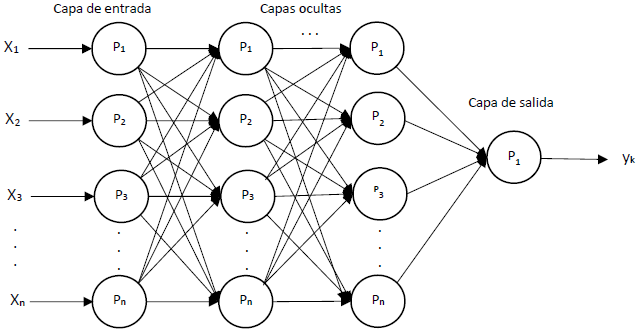
\includegraphics[width=0.8\textwidth]{images/rna.png}
    \caption{Estructura general de una Red Neuronal Artificial}
    \label{fig:rna}
\end{figure}

\justify
Una ANN está compuesta por nodos llamados neuronas, que se conectan entre sí mediante enlaces denominados \textit{sinapsis}. Estas conexiones determinan cómo se transmite la información y, en conjunto, definen el comportamiento de la red. En la Figura~\ref{fig:rna} se observa un ejemplo con dos capas ocultas, donde $X_n$ representan las variables de entrada, $y_n$ las salidas y $\varphi$ la función de activación.
\justify
Cada neurona se conecta con otras a través de sinapsis cuyo peso, representado por $W_{ji}$, refleja la fuerza o importancia de la conexión. La Ecuación~\ref{eq:neurona_salida} expresa matemáticamente cómo se calcula la salida de una neurona: las entradas $x_n$ son ponderadas por los pesos $W_{ji}$ y transformadas mediante la función de activación $\varphi$. Además, cada neurona posee un valor umbral que ajusta su nivel de respuesta.

\begin{equation}
    y_{i} = \varphi \left( \sum_{i=0}^{n} W_{ji}x_{i} \right)
    \label{eq:neurona_salida}
\end{equation}

\subsection{Recurrent Neural Network (RNN)}
\justify
Las Redes Neuronales Recurrentes (RNN) surgieron en la década de 1980, aunque su aplicación práctica se ha expandido recientemente gracias al incremento del poder computacional proporcionado por las unidades de procesamiento gráfico. Estas redes resultan especialmente útiles para el tratamiento de datos secuenciales, ya que cada neurona o unidad posee una memoria interna que le permite retener información sobre las entradas previas. A diferencia de las redes neuronales tradicionales, las RNN incorporan bucles de retroalimentación que permiten transferir información entre neuronas mientras se procesan las secuencias de entrada \cite{lazzeri2020machine}.
\justify
Las RNNs son un tipo de red que mantiene información de pasos anteriores mediante bucles internos y estados ocultos, lo que les permite recordar y aprovechar el contexto pasado. 
Mientras que las redes tradicionales aprenden únicamente de los datos actuales, las RNNs integran el estado oculto como una forma de memoria que se actualiza con cada nueva entrada.
Esta memoria, almacenada en un vector, se combina con el nuevo dato de entrada para producir una salida (Y) y actualizar el estado interno, como se muestra en la Figura \ref{fig:rnn}.

\begin{figure}[H]
    \centering
    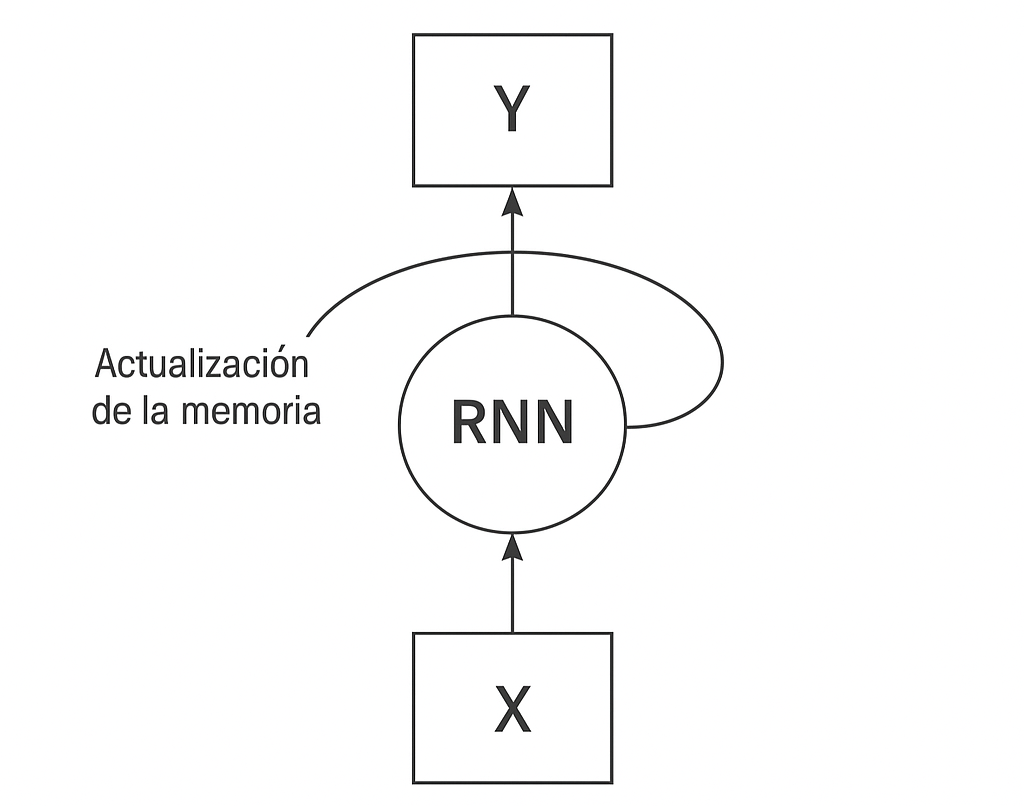
\includegraphics[width=0.4\textwidth]{images/rnn.png}
    \caption{Estructura de una Red Neuronal Recurrente (RNN)}
    \label{fig:rnn}
\end{figure}

\justify
Las unidades de una RNN se denominan \textit{unidades recurrentes} porque el valor actual depende de manera recurrente de los eventos previos. Este comportamiento puede interpretarse como la existencia de múltiples copias del mismo nodo, cada una transmitiendo información de forma secuencial hacia su sucesor. Esta relación recursiva se ilustra en la Figura~\ref{fig:rnn_arc}.

\begin{figure}[H]
    \centering
    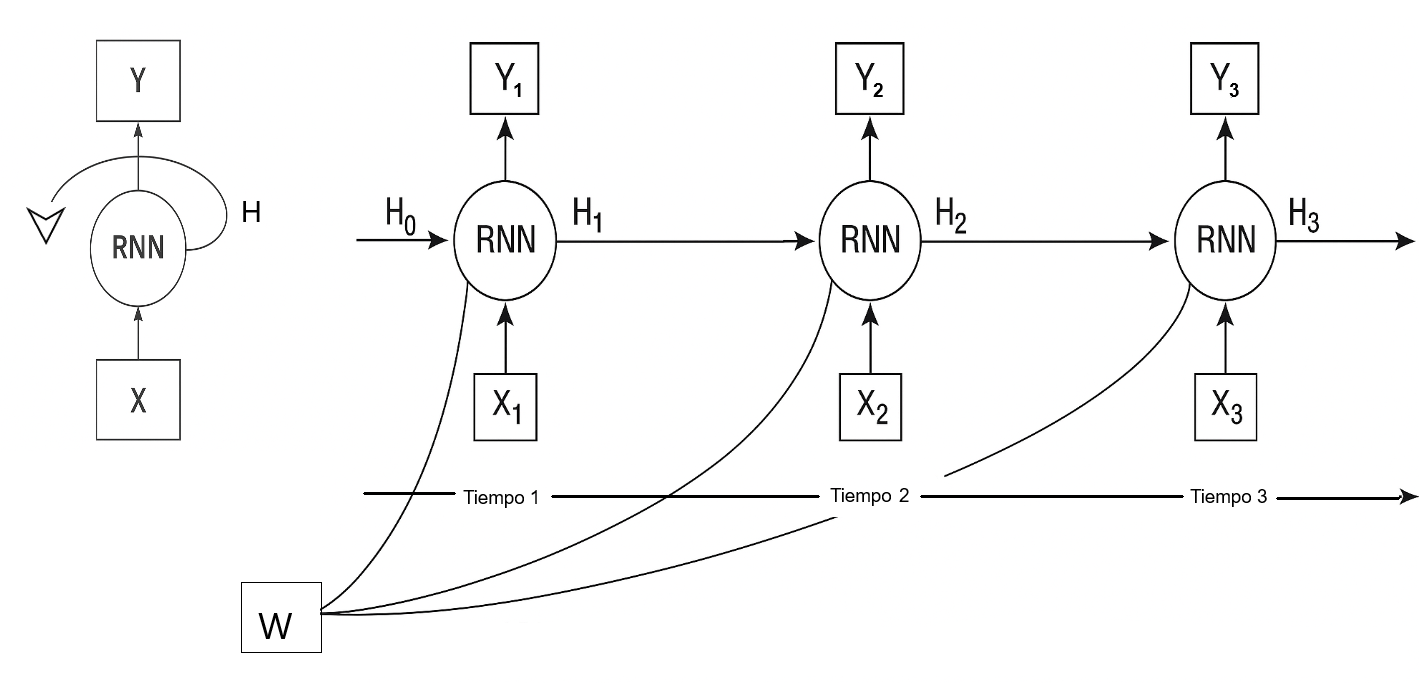
\includegraphics[width=0.6\textwidth]{images/rnn_arc.png}
    \caption{Arquitectura de una Red Neuronal Recurrente (RNN)}
    \label{fig:rnn_arc}
\end{figure}

\justify
En la Figura~\ref{fig:rnn_arc} se representa la arquitectura de una RNN. Este tipo de red posee un estado interno oculto, denotado como $H$, que puede retroalimentarse dentro de la propia red. La RNN procesa los valores de entrada $X$ y genera valores de salida $Y$. El estado oculto $H$ permite que la información se propague de un nodo a otro dentro de la red, organizándose en secuencias o vectores que contienen información tanto de la entrada actual como de las anteriores. Posteriormente, dicho vector pasa por la función de activación tangente hiperbólica ($\tanh$), que regula los valores dentro del rango $[-1,1]$.

\justify
Cada unidad cuenta con tres conjuntos de pesos: uno para las entradas ($X$), otro para los estados ocultos previos ($H$) y otro para las salidas ($Y$). Estos pesos se ajustan durante el proceso de entrenamiento mediante el método de descenso del gradiente, el cual actualiza los parámetros minimizando una función de pérdida. 

\subsection{Long Short-Term Memory (LSTM)}
\justify
Las redes LSTM, introducidas por Hochreiter y Schmidhuber \cite{hochreiter1997long}, constituyen una variante de las RNNs desarrollada con el propósito de superar las limitaciones de estas últimas al aprender dependencias de largo plazo en secuencias.
En los modelos RNN convencionales, la información se transmite a través de los estados ocultos a lo largo del tiempo, pero durante el proceso de entrenamiento basado en retropropagación a través del tiempo (BPTT) los gradientes tienden a desvanecerse o explotar.
Este fenómeno impide que las RNN aprendan eficazmente relaciones entre eventos temporalmente distantes.
\justify
El modelo LSTM introduce una unidad de memoria interna, denominada celda, que puede mantener información constante a lo largo de múltiples pasos temporales, resolviendo de manera efectiva el problema del desvanecimiento del gradiente.
Cada celda incluye un estado interno $C_t$ y un estado oculto $H_t$, junto con un conjunto de compuertas multiplicativas que regulan el flujo de información.
\justify
El principio clave es que el estado interno posee una autoconexión de peso fijo igual a 1, lo cual garantiza que los gradientes puedan fluir a través del tiempo sin desaparecer, manteniendo la información relevante.
\subsubsection{Compuertas del LSTM}
\justify
Cada celda LSTM cuenta con tres compuertas principales: entrada, olvido y salida.
\justify
Estas compuertas controlan de manera diferenciada cómo se actualiza y utiliza la información almacenada en la celda:

\begin{itemize}
\item Puerta de entrada $I_t$: regula cuánta información nueva proveniente de la entrada actual $X_t$ se incorpora al estado interno.
\item  Puerta de olvido $F_t$: decide qué fracción del estado anterior $C_{t-1}$ se conserva o se descarta.
\item  Puerta de salida $O_t$: determina cuánto del estado interno actualizado influirá en la salida del modelo $H_t$.
\end{itemize}

\justify
Cada una de estas compuertas se calcula mediante una capa completamente conectada seguida de una función sigmoide, que restringe los valores al intervalo (0, 1). Matemáticamente, para un conjunto de $n$ observaciones y $h$ unidades ocultas, las compuertas se definen como:

\begin{equation}
I_t = \sigma(X_t W_{xi} + H_{t-1} W_{hi} + b_i) \
\end{equation}

\begin{equation}
F_t = \sigma(X_t W_{xf} + H_{t-1} W_{hf} + b_f) \
\end{equation}

\begin{equation}
O_t = \sigma(X_t W_{xo} + H_{t-1} W_{ho} + b_o)
\end{equation}

\justify
donde $W_{xi}, W_{xf}, W_{xo} \in \mathbb{R}^{d \times h}$ y $W_{hi}, W_{hf}, W_{ho} \in \mathbb{R}^{h \times h}$ son las matrices de pesos asociados a la entrada y al estado oculto previo respectivamente, mientras que $b_{i}, b_{f}, b_{o} \in \mathbb{R}^{1 \times h}$ representa los sesgos.

\subsubsection{Estado candidato y actualización del estado interno}
\justify
Además de las compuertas, la celda genera un estado candidato $\tilde{C}_t$, que representa la nueva información potencial a incorporar al estado interno.
Este se obtiene aplicando una activación tangente hiperbólica $(\tanh)$ sobre una combinación lineal de la entrada y el estado oculto previo:

\begin{equation}
\tilde{C}_t = \tanh(X_t W_{xc} + H_{t-1} W_{hc} + b_c)
\end{equation}

\justify
Posteriormente, el estado interno de la celda $C_t$ se actualiza combinando la información retenida y la información nueva de acuerdo con:

\begin{equation}
C_t = F_t \odot C_{t-1} + I_t \odot \tilde{C}_t
\end{equation}

\justify
donde $\odot$ representa el producto elemento a elemento (Hadamard).
\justify
En este esquema, la puerta de olvido controla cuánto del estado anterior se preserva, mientras que la puerta de entrada modula cuánto de la nueva información se añade.
Si $F_t = 1$ y $I_t = 0$, la celda retiene íntegramente la información anterior, actuando como una memoria persistente.

\subsubsection{Generación del estado oculto}
\justify
El estado oculto de salida $H_t$ es la señal que se propaga a las capas siguientes o al paso temporal siguiente dentro de la secuencia.
\justify
Se obtiene aplicando una función tangente hiperbólica al estado interno actualizado y modulando el resultado mediante la puerta de salida:

\begin{equation}
H_t = O_t \odot \tanh(C_t)
\end{equation}

\justify
Este mecanismo permite que el modelo decida en qué momentos la información almacenada en la celda debe influir en la salida, y en qué momentos debe permanecer “oculta”, manteniendo la información sin propagarla.
\justify
La Figura \ref{fig:lstmcell} ilustra la estructura interna de una celda de memoria LSTM. En ella se observa cómo las compuertas de entrada $I_t$, olvido $F_t$ y salida $O_t$ regulan el flujo de información a través del estado interno de la celda $C_t$.
\justify
La compuerta de entrada controla cuánta información nueva proveniente de la entrada $X_t$ se incorpora, mientras que la compuerta de olvido determina qué parte del estado previo $C_{t-1}$ debe descartarse. Finalmente, la compuerta de salida define qué proporción del estado interno actualizado influye en la salida del modelo $H_t$.

\begin{figure}[H]
    \centering
    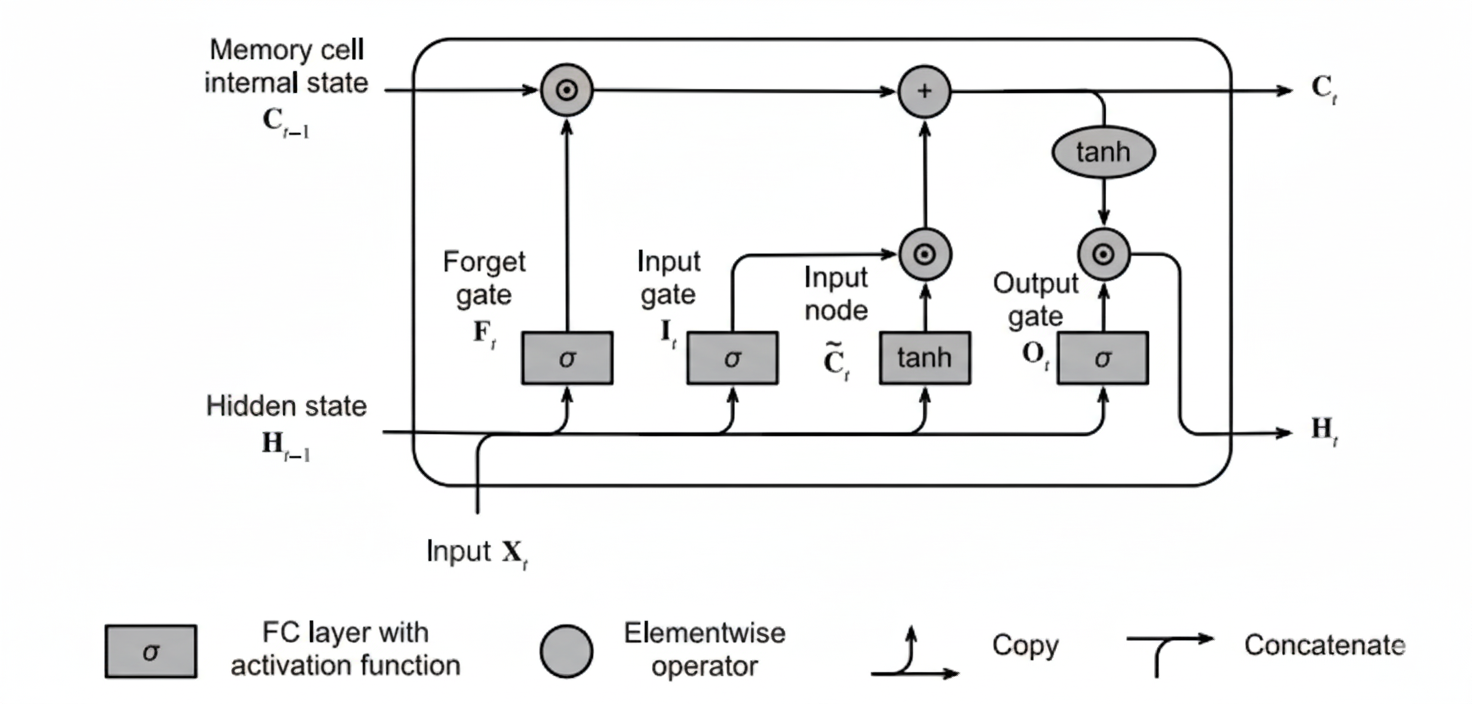
\includegraphics[width=0.8\textwidth]{images/lstm_cell.png}
    \caption{Estructura interna de una celda de memoria LSTM.} 
    \label{fig:lstmcell}
\end{figure}

\subsection{Gated Recurrent Unit (GRU)}
\justify
Las redes GRU fueron introducidas por Cho et al. \cite{cho2014learning} como una simplificación del modelo LSTM. El objetivo fue conservar la capacidad de las redes recurrentes para modelar dependencias a largo plazo, reduciendo al mismo tiempo la complejidad computacional y el número de parámetros.
\justify
A diferencia de las LSTM, las GRU fusionan el estado de la celda y el estado oculto en una única representación, lo que las hace más eficientes sin sacrificar desempeño en la mayoría de los problemas de predicción secuencial.
\subsubsection{Estructura general}
\justify
La arquitectura GRU incorpora dos compuertas principales:
\begin{itemize}
\item Compuerta de reinicio (reset gate), que controla cuánta información del estado previo debe olvidarse.
\item Compuerta de actualización (update gate), que determina en qué medida se conserva la información anterior o se actualiza con la nueva entrada.
\end{itemize}
\justify
Ambas compuertas se activan mediante funciones sigmoides, lo que restringe sus valores al rango (0, 1).

\subsubsection{Compuertas de reinicio y actualización}
\justify
Sea $X_t \in \mathbb{R}^{n \times d}$ el vector de entrada en el instante $t$, donde $n$ representa el tamaño del lote y $d$ la dimensión de las variables de entrada.
\justify
Sea además $H_{t-1} \in \mathbb{R}^{n \times h}$ el estado oculto proveniente del paso temporal anterior, con $h$ unidades ocultas.
\justify
La compuerta de reinicio $R_t \in \mathbb{R}^{n \times h}$ y la compuerta de actualización $Z_t \in \mathbb{R}^{n \times h}$ se calculan como:

\begin{equation}
R_t = \sigma(X_t W_{xr} + H_{t-1} W_{hr} + b_r)
\end{equation}

\begin{equation}
Z_t = \sigma(X_t W_{xz} + H_{t-1} W_{hz} + b_z)
\end{equation}

\justify
donde $W_{xr}, W_{xz} \in \mathbb{R}^{d \times h}$ y $W_{hr}, W_{hz} \in \mathbb{R}^{h \times h}$ son matrices de pesos, mientras que $b_r, b_z \in \mathbb{R}^{1 \times h}$ son los términos de sesgo (\textit{bias}).
\justify
Las funciones sigmoides $\sigma(\cdot)$ garantizan que cada componente de las compuertas adopte valores entre 0 y 1, controlando el grado de influencia de la información anterior y la nueva.

\justify
Intuitivamente:
\begin{itemize}
\item Cuando $R_t$ toma valores cercanos a 0, la red tiende a olvidar información previa, reiniciando parte del estado.
\item Cuando $Z_t$ se aproxima a 1, la red adopta el nuevo estado candidato, actualizando la información con la entrada actual.
\end{itemize}

\subsubsection{Estado oculto candidato}

\justify
La compuerta de reinicio regula la combinación entre la información previa y la nueva entrada.
\justify
Integrando este comportamiento, se define un estado oculto candidato $\tilde{H}_t \in \mathbb{R}^{n \times h}$ como:

\begin{equation}
\tilde{H}_t = \tanh(X_t W_{xh} + (R_t \odot H_{t-1}) W_{hh} + b_h)
\end{equation}

\justify
donde $W_{xh} \in \mathbb{R}^{d \times h}$ y $W_{hh} \in \mathbb{R}^{h \times h}$ son matrices de pesos, $b_h \in \mathbb{R}^{1 \times h}$ son los términos de sesgo (\textit{bias}), el símbolo $\odot$ indica el producto de Hadamard, es decir, una multiplicación elemento a elemento, y la función de activación $\tanh$ limita los valores del estado candidato al intervalo $(-1,1)$.

\justify
En este paso, la compuerta $R_t$ decide cuánto del estado oculto previo $H_{t-1}$ debe combinarse con la nueva información $X_t$.
Si $R_t$ es cercano a cero, el modelo tiende a ignorar el pasado, comportándose como una red neuronal multicapa convencional.
Por el contrario, si $R_t$ es cercano a uno, el modelo retiene información previa, asemejándose a un RNN estándar.

\subsubsection{Actualización del estado oculto}
\justify
Finalmente, la compuerta de actualización $Z_t$ controla el equilibrio entre el estado anterior y el nuevo candidato.
\justify
El estado oculto final $H_t$ se calcula como:

\begin{equation}
H_t = (1 - Z_t) \odot H_{t-1} + Z_t \odot \tilde{H}_t
\end{equation}  

\justify
donde $Z_t$ actúa como un mecanismo de interpolación entre el pasado y el presente.

\begin{itemize}
\item Si $Z_t \approx 1$, el modelo adopta completamente el nuevo estado candidato $\tilde{H}_t$, actualizando la información.
\item Si $Z_t \approx 0$, el modelo mantiene la memoria previa $H_{t-1}$, ignorando la entrada actual.
\end{itemize}

\justify
Este diseño permite a las GRU manejar eficientemente dependencias a corto y largo plazo, ya que:

\begin{itemize}
\item La compuerta de reinicio captura relaciones de corto plazo, al controlar el olvido parcial;
\item La compuerta de actualización permite retener información de largo plazo, al preservar estados relevantes.
\end{itemize}

\justify
La Figura \ref{fig:grucell} representa la estructura interna de una celda GRU. 
A diferencia de la arquitectura LSTM, la GRU combina las funciones de las compuertas de entrada y olvido en una sola compuerta de actualización $Z_t$, y utiliza además una compuerta de reinicio $R_t$ que controla la influencia del estado previo $H_{t-1}$ en el cálculo del nuevo estado candidato $\tilde{H}_t$.

\justify
De esta manera, la GRU logra capturar dependencias temporales a largo plazo con una estructura más simple y menos parámetros que la LSTM.

\begin{figure}[H]
    \centering
    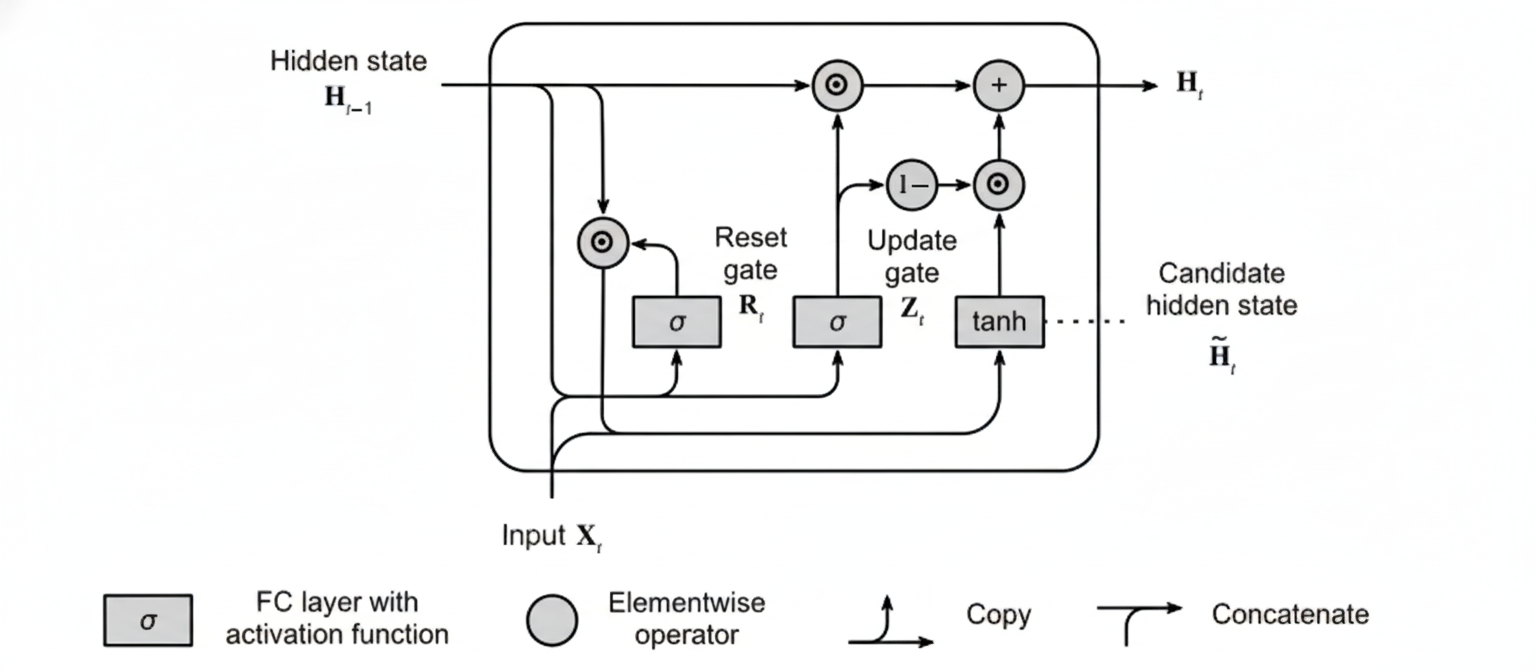
\includegraphics[width=0.8\textwidth]{images/gru_cell.png}
    \caption{Estructura interna de una celda de memoria GRU.}
    \label{fig:grucell}
\end{figure}

\section{Índices de rendimiento}

\justify
Para evaluar el desempeño de un modelo predictivo, se recurre al uso de métricas estadísticas que permiten cuantificar la precisión de las estimaciones realizadas respecto a los valores observados. 

\justify
En este trabajo se emplea como medida principal la \textit{Raíz del Error Medio Cuadrático} (\textit{Root Mean Squared Error} – RMSE), ampliamente utilizada en problemas de predicción y regresión por su capacidad de reflejar la magnitud promedio de los errores de predicción.

\justify
El RMSE evalúa la diferencia promedio entre los valores reales $y_i$ y los valores estimados $\hat{y}_i$ generados por el modelo, penalizando de forma más severa los errores de gran magnitud debido a la elevación al cuadrado de las diferencias. Su formulación matemática se expresa como:

\begin{equation}
    RMSE = \sqrt{\frac{1}{n} \sum_{i=1}^{n} (y_i - \hat{y}_i)^2}
\end{equation}

\justify
donde $n$ representa el número total de observaciones, $y_i$ el valor observado y $\hat{y}_i$ el valor predicho correspondiente. El resultado del RMSE se expresa en las mismas unidades que la variable analizada, lo cual facilita su interpretación directa.

\justify
Un valor de RMSE igual a cero indica un ajuste perfecto entre los valores reales y las predicciones, mientras que valores más elevados reflejan un menor grado de precisión del modelo. En este sentido, el RMSE constituye un indicador robusto para comparar el desempeño de diferentes modelos predictivos, permitiendo identificar aquel que logra minimizar el error medio en las estimaciones.


% 3. Metodología
\chapter{Metodología}
\thispagestyle{empty}
\vspace{0.5cm}
\section{Recolección y preprocesamiento de datos}
\vspace{0.5cm}
\justify
Para este estudio se consideraron los precios promedio mensuales de tres materiales de construcción representativos del mercado nacional: cemento de la marca Yguazú, cal hidratada de la marca Impacal y ladrillo común de la marca Tobatí.

\justify
Los datos fueron obtenidos de la revista técnica Mandu’a \cite{mandua}, especializada en el sector de la construcción, de distribución gratuita y publicación mensual. Esta fuente constituye un referente técnico en Paraguay para el seguimiento de precios de materiales y tendencias del mercado.

\justify
Adicionalmente, se incorporó como variable exógena el nivel del río Paraguay, cuyos registros diarios fueron extraídos de la página oficial de la Dirección de Meteorología e Hidrología \cite{dmh}. 

\justify
Tras la recopilación de los datos diarios, se extrajo para cada mes el nivel mínimo registrado, generando así una serie mensual del nivel del río que mantiene correspondencia temporal con la serie mensual de precios de los materiales de construcción.

\justify
El trabajo se desarrolló en tres etapas principales:
\begin{itemize}
\item Recolección y preprocesamiento de datos, que incluyó la integración, limpieza y tratamiento de valores faltantes.
\item Predicción del nivel del río Paraguay mediante un modelo LSTM univariado unistep, utilizado posteriormente como variable exógena en los modelos predictivos de precios de materiales de construcción.
\item Construcción y evaluación de modelos predictivos, en los cuales se aplicaron y compararon los enfoques SARIMAX, LSTM y GRU para estimar la evolución de los precios de los materiales seleccionados.
\end{itemize}

\justify
El conjunto de datos para los precios del cemento, la cal hidratada y el ladrillo común comprenden el período enero de 2014 a julio de 2025. Este intervalo se definió debido a que la Revista Técnica Mandu’a \cite{mandua} pone a disposición registros históricos únicamente desde el año 2014 en su sitio web.

\justify
En cuanto al nivel del río Paraguay en el puerto de Asunción se utilizaron registros desde enero de 1990 hasta julio de 2025. Este intervalo se eligió siguiendo las recomendaciones de la Organización Meteorológica Mundial (OMM), que establece que para estudios hidrológicos y climáticos es adecuado considerar un período de al menos 30 años, lo que permite capturar la variabilidad natural de largo plazo y obtener una representación más robusta del comportamiento histórico del río \cite{EstudioClimaParaguay2019}.

\justify
Durante la recolección de los datos de precios se identificó que, para algunos meses, no se disponía del valor promedio correspondiente. Con el fin de garantizar la continuidad temporal de las series y permitir la correcta aplicación de los modelos predictivos, se evaluaron distintos métodos de interpolación \cite{conesa2011interpolacion} para el tratamiento de los datos faltantes utilizando la función interpolate de la librería pandas, entre ellos:

\begin{itemize}
\item Interpolación lineal, que estima los valores intermedios a partir de una conexión recta entre los puntos adyacentes conocidos.
\item Interpolación polinómica de orden 2 y orden 3, que ajusta curvas polinómicas de segundo y tercer grado respectivamente, permitiendo capturar tendencias locales más suavizadas.
\item Interpolación spline cúbica y de orden 3, que genera curvas suaves mediante funciones polinómicas por tramos, adecuadas para representar variaciones continuas sin generar quiebres abruptos.
\item Interpolación basada en el tiempo (time-based), que utiliza el índice temporal como referencia para la estimación de los valores faltantes.
seleccionados.
\end{itemize}

\justify
Una vez realizado el análisis comparativo de los métodos de interpolación, se seleccionó la interpolación polinómica cuadrática para el tratamiento de los precios faltantes, dado que este método mostró la mejor aproximación a los valores reales proporcionados por la empresa de compra y venta de materiales de construcción Edylur \cite{edylur}. Esta técnica permitió preservar la suavidad de la serie y capturar adecuadamente las tendencias locales sin generar variaciones abruptas, asegurando así la coherencia y estabilidad de las series temporales utilizadas por los modelos SARIMAX, LSTM y GRU en las etapas posteriores del estudio.
\section{Modelado y Predicción de Series Temporales}

\justify
El problema de predicción que aborda este trabajo tiene una particularidad que condiciona las decisiones metodológicas: las series de precios son cortas (poco más de 130 observaciones mensuales), no lineales, y están influenciadas por variables externas de naturaleza distinta — una hidrológica y otra socioeconómica. Esa combinación descarta algunos enfoques sencillos y justifica el uso paralelo de un modelo estadístico clásico y dos arquitecturas de redes neuronales recurrentes.

\justify
La estrategia adoptada fue secuencial: primero se proyectó el nivel del río Paraguay a través de un LSTM univariado —aprovechando la serie histórica diaria desde 1990—, y luego esa proyección se incorporó como variable exógena en los modelos de predicción de precios. Esta cadena permite que la información hidrológica sea explícita en el proceso de pronóstico, en lugar de quedar implícita o ignorada.

\subsection{Modelo Long Short-Term Memory (LSTM) para la predicción del Nivel del Río Paraguay}
\justify
Para predecir el nivel mensual del río Paraguay se utilizó un modelo LSTM univariado unistep, reconocido por su eficacia en series temporales hidrológicas. Estudios muestran que LSTM supera a modelos clásicos como ARIMA, reduciendo errores hasta en un 87\% en series no lineales \cite{siami2018}, y presenta alta precisión en predicciones fluviales \cite{kratzert2018}\cite{kratzert2019}. Frente a GRU, LSTM es más efectivo en dependencias de largo plazo \cite{YUNITA2025103462}, y también supera a arquitecturas Transformer en métricas como NSE y KGE para predicción diaria \cite{liu2023}. Con cerca de 8.000 observaciones diarias y un horizonte de 24 meses, LSTM ofrece un balance adecuado entre precisión y robustez para este dominio.
\justify
Los datos se escalaron en el rango [-1, 1] mediante el método MinMaxScaler, con el objetivo de mejorar la estabilidad numérica y favorecer la convergencia durante el entrenamiento.
\justify
Se generaron secuencias supervisadas utilizando una ventana deslizante, lo que permitió al modelo capturar los patrones de dependencia temporal del nivel del río. Finalmente, los datos se dividieron cronológicamente en tres subconjuntos: 80\% para entrenamiento, 10\% para validación y 10\% para prueba, asegurando que el conjunto de prueba representara las observaciones más recientes de la serie.1
\justify
Los hiperparámetros del modelo, incluyendo el número de neuronas, la tasa de aprendizaje y el número de épocas, fueron seleccionados mediante la librería Optuna, que permite realizar una búsqueda automática y eficiente del conjunto de parámetros que minimiza el error de validación.

\subsection{Modelo Seasonal AutoRegressive Integrated Moving Average with eXogenous variables (SARIMAX) para la predicción de precios de Materiales de Construcción}

\justify
Se aplicó el modelo SARIMAX para predecir los precios mensuales del cemento, la cal hidratada y el ladrillo común, considerando como variables exógenas el nivel mensual del río Paraguay —estimado previamente mediante un modelo LSTM univariado— y el confinamiento por covid-19 representada de forma binaria, que representa los períodos de restricción sanitaria durante la pandemia.

\justify
Para cada material de construcción, el conjunto de datos se dividió en entrenamiento y prueba, utilizando los últimos 12 meses como segmento de validación. La selección de los parámetros óptimos (p,d,q)(P,D,Q,s) se realizó mediante la función pmdarima.auto\_arima, que efectúa una búsqueda iterativa de combinaciones de órdenes con el fin de minimizar el AIC y optimizar el desempeño del modelo en términos de RMSE [15].

\justify
A fin de evaluar el impacto del confinamiento por covid-19, se elaboraron predicciones a 24 meses bajo dos escenarios comparativos:

\begin{itemize}
\item Escenario 1 – Sin confinamiento: la variable exógena Confinamiento\_Covid se fijó en 0 para todo el horizonte de predicción.

\item Escenario 2 – Con confinamiento: la variable exógena Confinamiento\_Covid se fijó en 1 para todo el período proyectado.
\end{itemize}

\justify
Esta estrategia permitió analizar el efecto potencial de eventos disruptivos —como restricciones sanitarias o logísticas— sobre la evolución de los precios de los materiales de construcción en Paraguay, integrando en el modelo tanto la influencia hidrológica como la económica.

\subsection{Modelos Long Short-Term Memory (LSTM) y Gated Recurrent Unit (GRU) para la predicción de precios de Materiales de Construcción}

\justify
Para la predicción de los precios mensuales del cemento, la cal hidratada y el ladrillo común, se implementaron modelos basados en redes neuronales recurrentes (RNN), específicamente las arquitecturas Long Short-Term Memory (LSTM) y Gated Recurrent Unit (GRU). Estos modelos son ampliamente utilizados en el tratamiento de series temporales no lineales, ya que permiten capturar dependencias de largo y corto plazo en los datos.

\justify
Ambos modelos se entrenaron utilizando las mismas variables:

\begin{itemize}
\item Variable objetivo: el precio promedio mensual de cada material.

\item Variables exógenas: el nivel mensual del río Paraguay y el confinamiento por COVID-19 (representado mediante una variable binaria).
\end{itemize}
\justify
El conjunto de datos, previamente interpolado y con el nivel del río consolidado y proyectado, fue escalado en el rango [-1, 1] mediante el método MinMaxScaler, con el fin de mejorar la estabilidad numérica y la convergencia durante el entrenamiento.

\justify
Se generaron secuencias supervisadas utilizando una ventana deslizante de 8 meses, lo que permitió que los modelos aprendieran los patrones de dependencia temporal entre las variables. Posteriormente, los datos fueron divididos cronológicamente en tres subconjuntos: 80\% para entrenamiento, 10\% para validación, y 10\% para prueba, garantizando que el conjunto de prueba representara las observaciones más recientes de la serie.


% 4. Resultados
\chapter{Resultados}
\thispagestyle{empty}
\section{Predicción del Nivel del Río Paraguay mediante LSTM}
\vspace{0.3cm}
\justify
Antes de construir los modelos de predicción de precios, se necesitaba contar con una proyección confiable del nivel del río Paraguay, variable que opera como entrada exógena en los modelos posteriores. Para esto se entrenó un modelo LSTM siguiendo tres etapas: búsqueda automática de hiperparámetros con Optuna, entrenamiento del modelo final con la configuración óptima y generación del pronóstico a 730 días consecutivos.

\subsection{Serie Histórica y Partición de los Datos}

\justify
La serie contiene registros diarios del nivel del río Paraguay en el Puerto de Asunción, abarcando el período de enero de 2014 a julio de 2025.

\justify
Las estadísticas descriptivas de la variable muestran una media de 2,63 m y una desviación estándar de 2,17 m, con valores entre $-1{,}61$ m y $7{,}88$ m. La Figura \ref{fig:serie_historica} muestra la serie completa, donde se aprecia la alternancia entre períodos de crecida y estiaje con amplitudes marcadamente distintas entre años.

\begin{figure}[H]
    \centering
    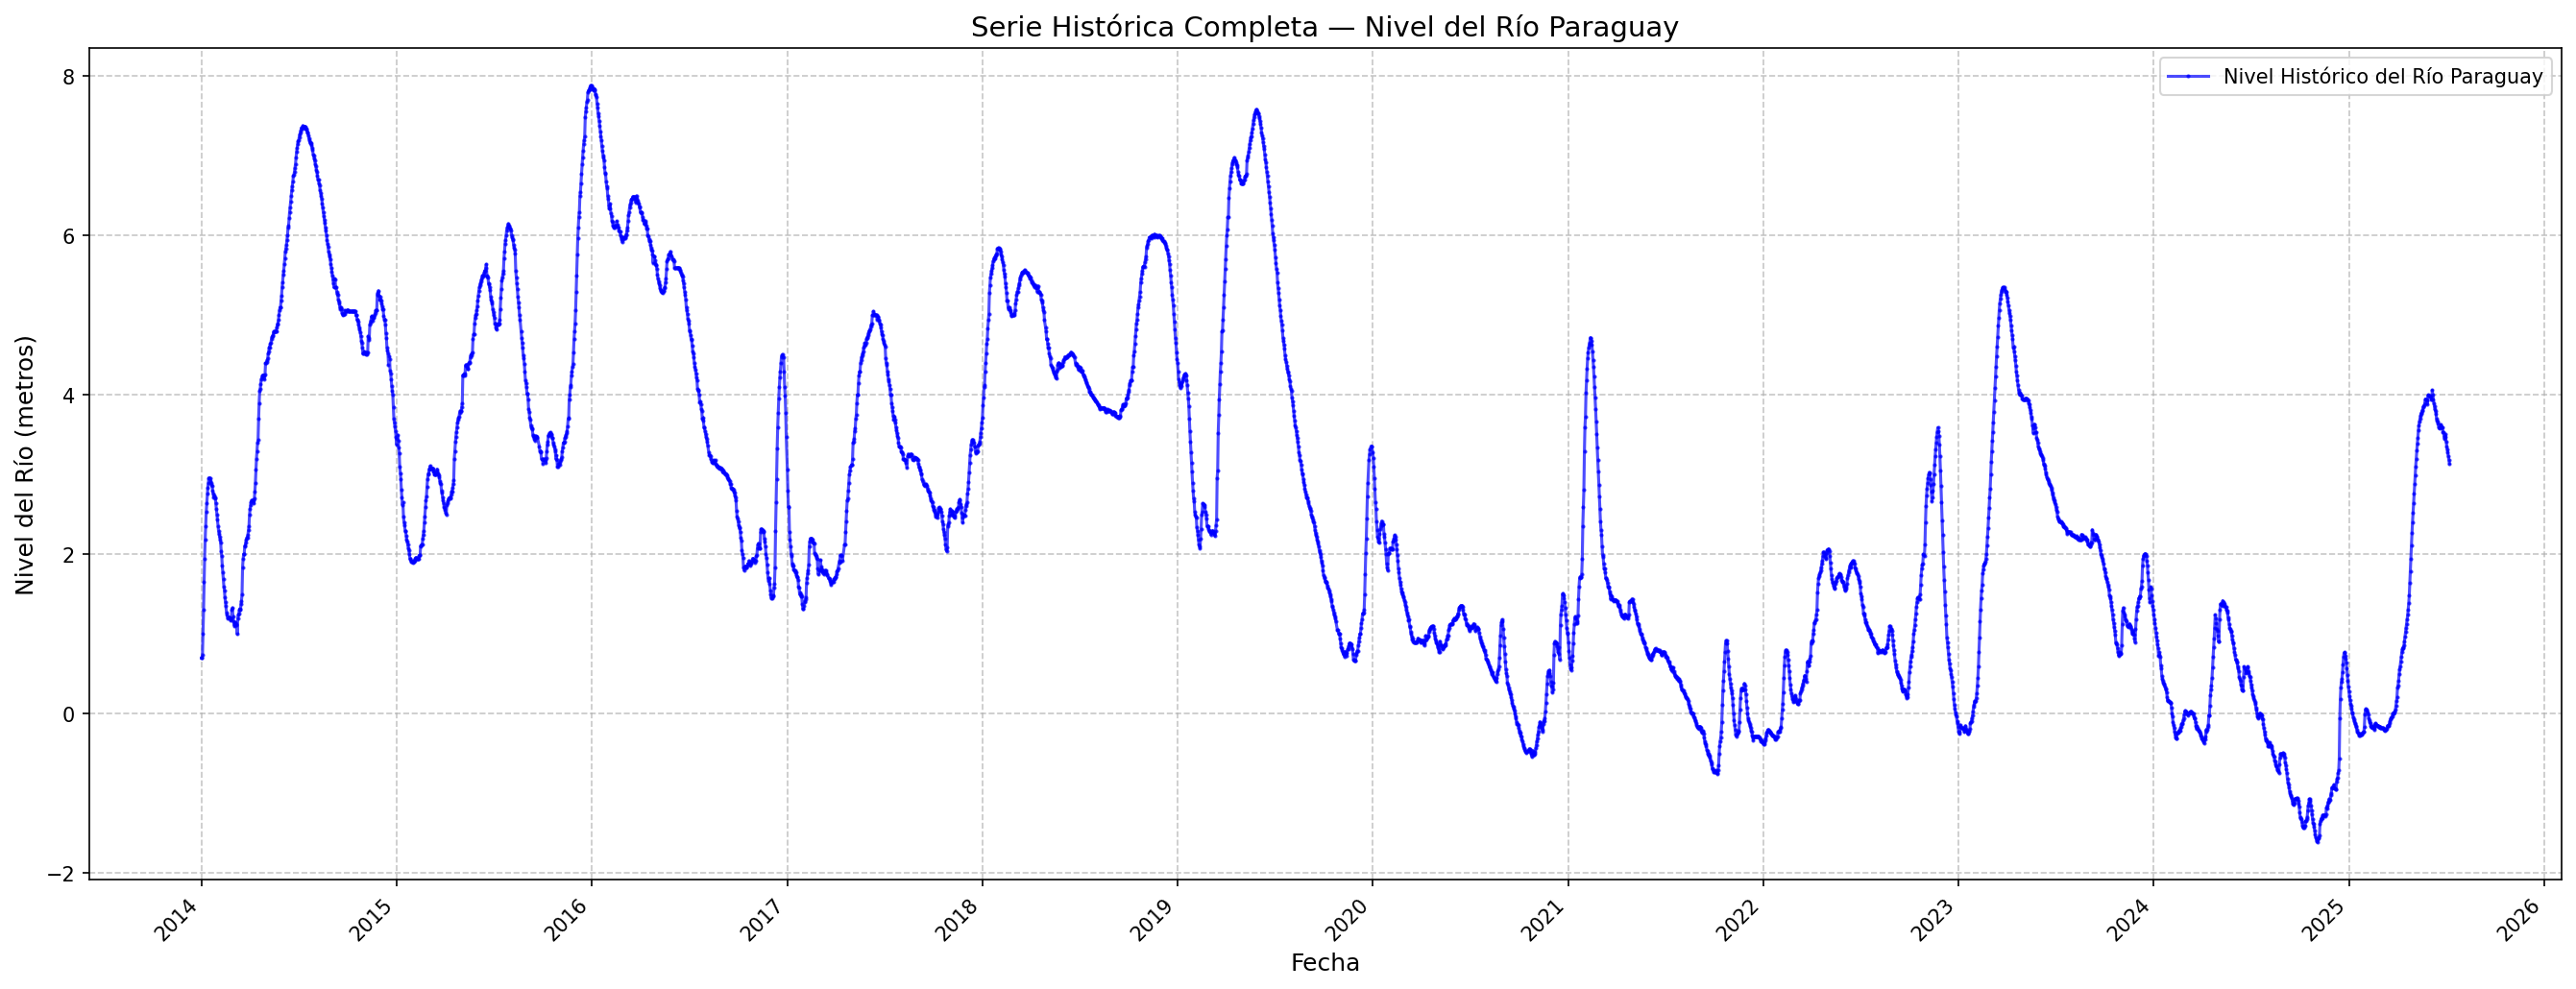
\includegraphics[width=\textwidth]{predicciones/prediccion_nivel_rio/resultados/grafico_00_serie_historica.png}
    \caption{Serie histórica completa del nivel diario del río Paraguay (2014--2025).}
    \label{fig:serie_historica}
\end{figure}

\justify
El modelo recibe 12 variables de entrada por paso de tiempo: el nivel del río más siete características temporales y cuatro de anomalía. Las temporales incluyen representaciones cíclicas del día del año, el mes y la estación (codificadas como seno y coseno), más el año normalizado. Las de anomalía capturan desviaciones respecto a medias móviles de 30 y 90 días, y tendencias de 7 y 30 días.

\justify
La partición del dataset siguió un criterio estrictamente cronológico. El conjunto de entrenamiento comprende desde el 1 de enero de 2014 hasta el 22 de enero de 2022 (2.944 observaciones, aproximadamente el 70\% del total); el de validación, desde el 23 de enero de 2022 hasta el 14 de octubre de 2023 (630 observaciones, el 15\%); y el de prueba, desde el 15 de octubre de 2023 hasta el 7 de julio de 2025 (632 observaciones, el 15\% restante). Al aplicar la ventana de lookback de 30 días al conjunto de entrenamiento, el número efectivo de secuencias se reduce a 2.914. Esta proporción fue seleccionada por ser la que produjo el mejor resultado en experimentos previos con distintas configuraciones de partición. La Figura \ref{fig:particiones} muestra la distribución temporal de los tres subconjuntos.

\begin{figure}[H]
    \centering
    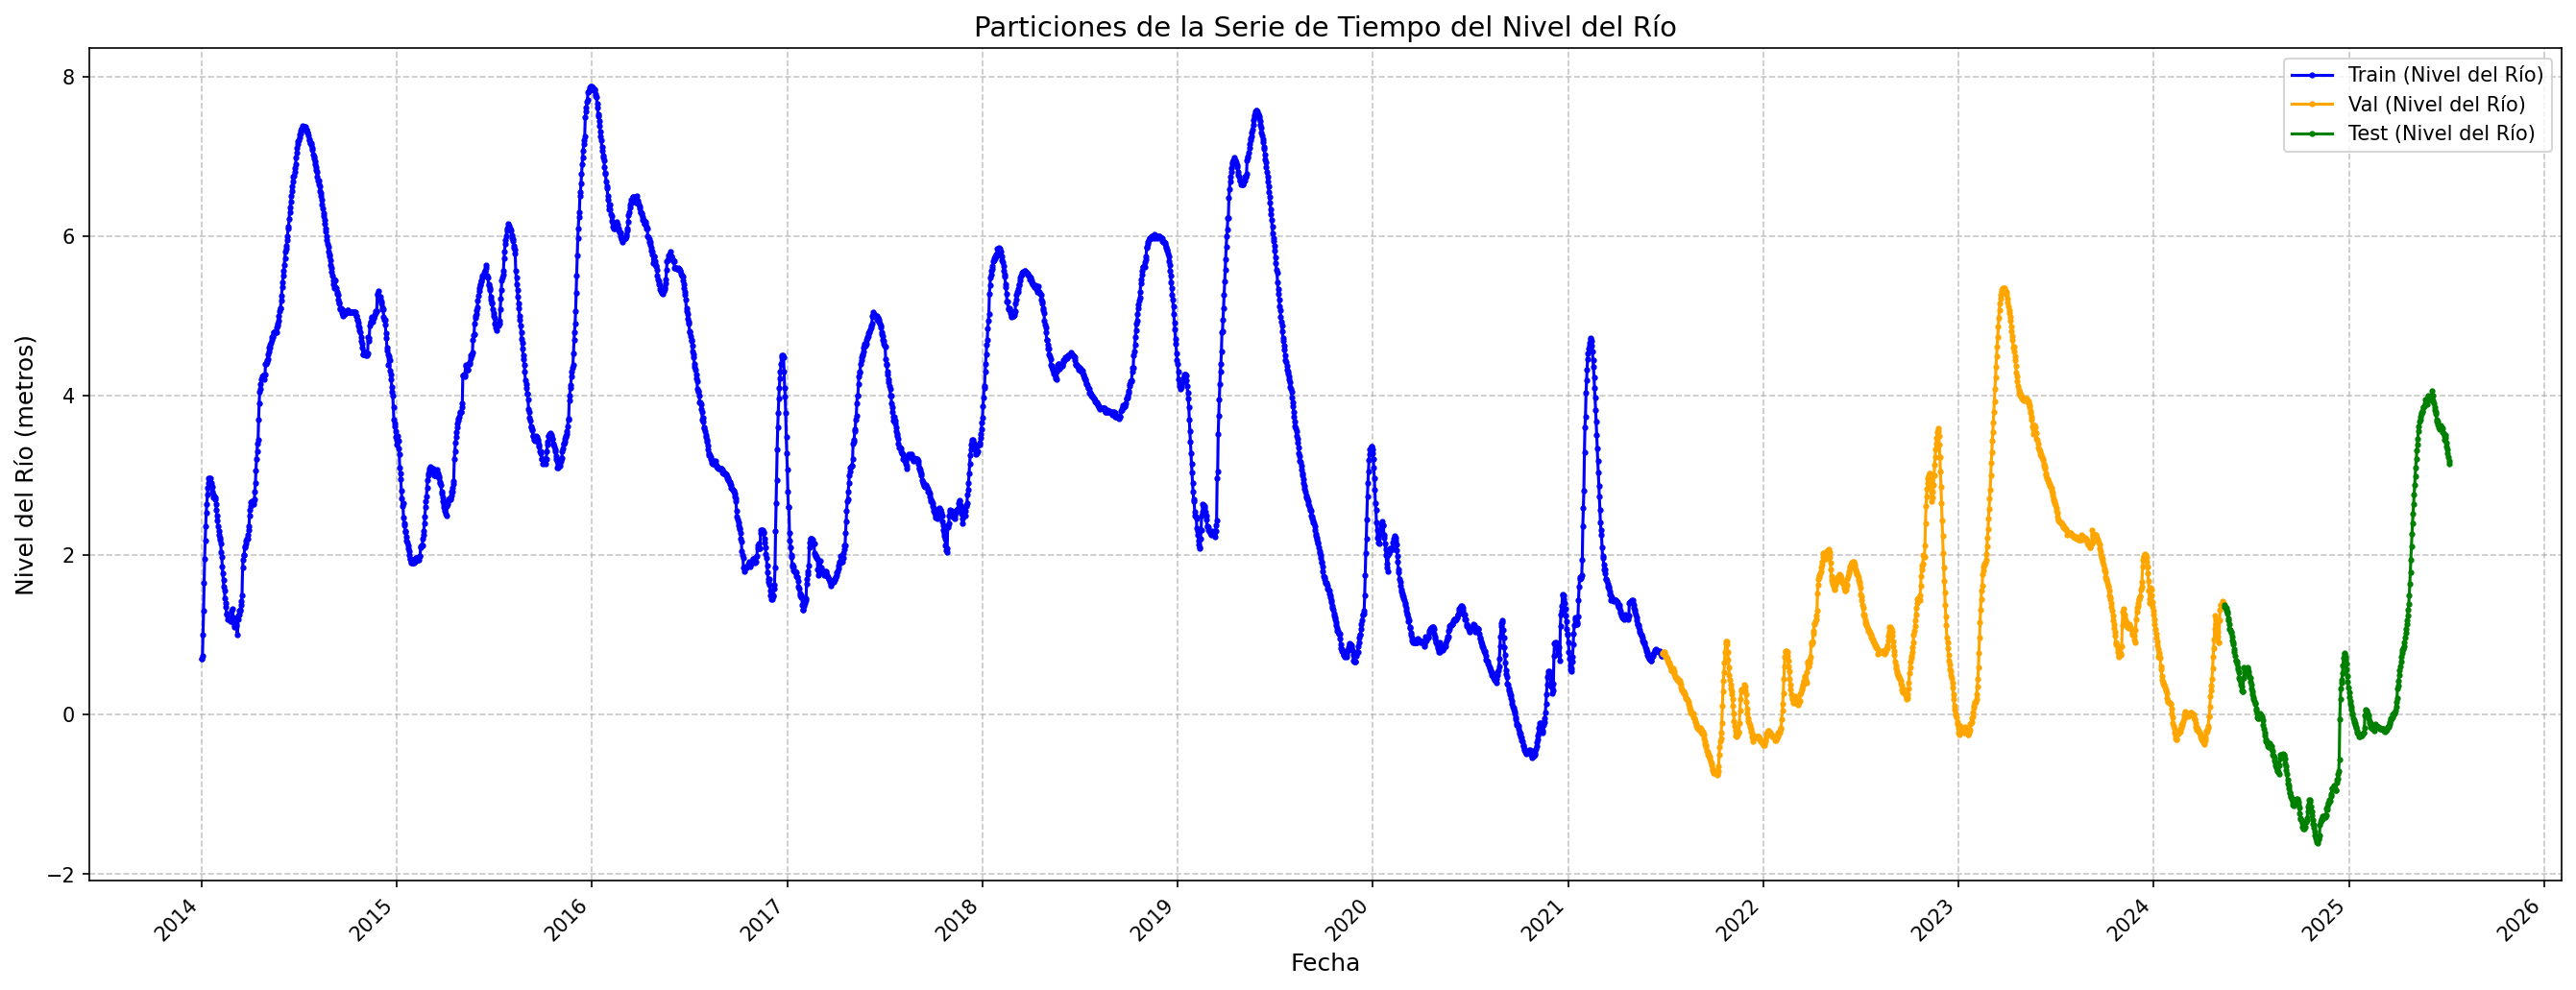
\includegraphics[width=\textwidth]{predicciones/prediccion_nivel_rio/resultados/grafico_01_particiones.png}
    \caption{Partición cronológica de la serie: entrenamiento (azul), validación (naranja) y prueba (verde).}
    \label{fig:particiones}
\end{figure}

\subsection{Optimización de Hiperparámetros con Optuna}

\justify
La búsqueda de hiperparámetros se realizó con Optuna, usando el sampler TPE (\textit{Tree-structured Parzen Estimator}) y poda de trials con \textit{MedianPruner} para descartar tempranamente las configuraciones claramente inferiores. Se evaluaron 300 trials, proceso que demandó 278 minutos en total. El mejor RMSE de validación obtenido fue de 0,0371 m.

\justify
Los hiperparámetros óptimos se resumen en la Tabla \ref{tab:hiperparametros_lstm_rio}.

\begin{table}[H]
    \centering
    \caption{Hiperparámetros óptimos del modelo LSTM para la predicción del nivel del río Paraguay.}
    \label{tab:hiperparametros_lstm_rio}
    \begin{tabular}{lc}
        \toprule
        \textbf{Hiperparámetro} & \textbf{Valor óptimo} \\
        \midrule
        Número de capas LSTM       & 1 \\
        Unidades ocultas           & 512 \\
        Bidireccional              & No \\
        Tasa de \textit{dropout}   & 0,05 \\
        Activación capa densa      & Lineal \\
        Ventana de lookback        & 30 días \\
        Estrategia de predicción   & Recursiva \\
        Optimizador                & Adam \\
        Tasa de aprendizaje        & 0,006079 \\
        \textit{Weight decay}      & $4{,}70 \times 10^{-7}$ \\
        Tamaño de lote (\textit{batch size}) & 256 \\
        Planificador de LR         & CosineAnnealingLR \\
        \bottomrule
    \end{tabular}
\end{table}

\justify
La configuración óptima corresponde a una sola capa LSTM con 512 unidades ocultas. La estrategia recursiva fue preferida sobre la directa, lo que indica que el modelo aprovecha mejor la retroalimentación acumulada paso a paso para proyecciones largas. El total de parámetros entrenables es de 1.075.713.

\subsection{Entrenamiento del Modelo Final}

\justify
El modelo final fue entrenado durante 99 épocas con los hiperparámetros óptimos, una ventana de lookback de 30 días y una paciencia de 30 épocas para la detención temprana. La Figura \ref{fig:curva_aprendizaje} presenta la evolución del error de entrenamiento y validación a lo largo del proceso.

\begin{figure}[H]
    \centering
    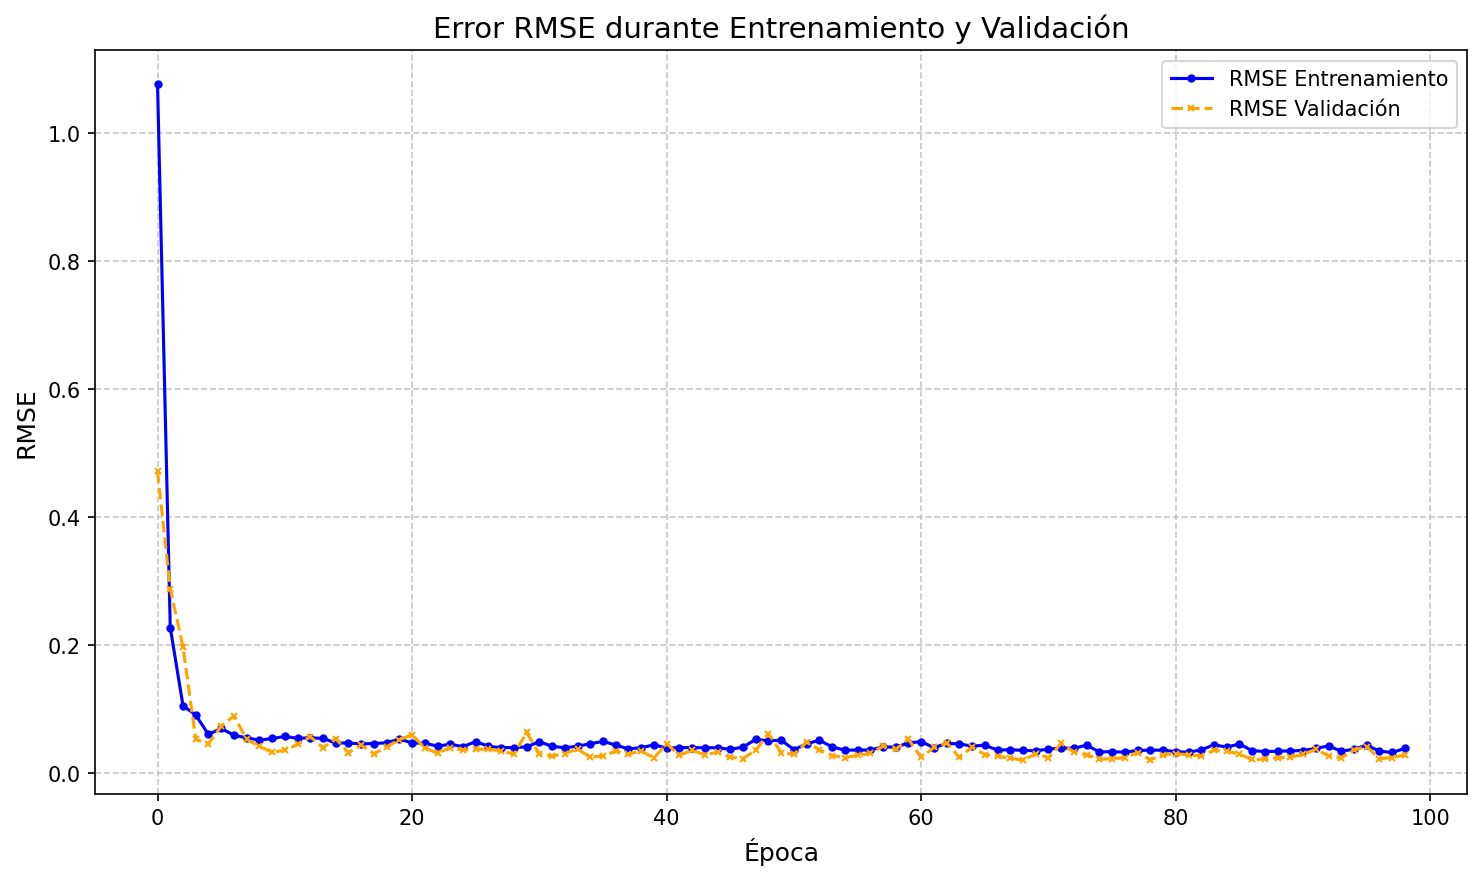
\includegraphics[width=0.85\textwidth]{predicciones/prediccion_nivel_rio/resultados/grafico_04_curva_aprendizaje.png}
    \caption{Curva de aprendizaje del modelo LSTM: RMSE de entrenamiento y validación por época.}
    \label{fig:curva_aprendizaje}
\end{figure}

\justify
Durante las primeras épocas, la pérdida cae rápidamente desde valores en torno a 0,30 hasta situarse por debajo de 0,10. A partir de la época 15 aproximadamente, el error de entrenamiento se estabiliza alrededor de 0,04 a 0,05, mientras el de validación oscila en rangos similares sin mostrar una tendencia ascendente sostenida, lo que indica que no se produjo sobreajuste significativo.

\subsection{Métricas de Evaluación}

\justify
La Tabla \ref{tab:metricas_lstm_rio} presenta el RMSE en los tres subconjuntos.

\begin{table}[H]
    \centering
    \caption{RMSE del modelo LSTM para el nivel del río Paraguay en los conjuntos de entrenamiento, validación y prueba.}
    \label{tab:metricas_lstm_rio}
    \begin{tabular}{lc}
        \toprule
        \textbf{Conjunto} & \textbf{RMSE (m)} \\
        \midrule
        Entrenamiento  & 0,0479 \\
        Validación     & 0,0373 \\
        Prueba         & 0,0457 \\
        \bottomrule
    \end{tabular}
\end{table}

\justify
El error en el conjunto de prueba es de 4,57 cm, sobre una variable que oscila entre $-1{,}61$ m y $7{,}88$ m. Este nivel de precisión, inferior a 5 cm sobre un rango de casi 10 metros, confirma la capacidad del modelo LSTM para reproducir la dinámica hidrológica del río Paraguay con alta fidelidad.

\subsection{Predicción del Nivel del Río a 730 Días}

\justify
Concluida la evaluación, se generó la predicción del nivel diario para un horizonte de 730 días mediante la estrategia recursiva: el modelo predice el valor del día siguiente ($t+1$) a partir de la ventana de 30 días previos, incorpora ese valor a la secuencia y repite el proceso hasta completar 730 pasos desde el último dato disponible (7 de julio de 2025, nivel = 3,14 m). Para reducir la acumulación de error en horizontes largos, la predicción se combina gradualmente con la climatología histórica a través de un factor de mezcla $\alpha(t)$ que decrece desde 1,00 en el primer paso hasta valores próximos a 0 hacia el final del horizonte ($\alpha = 0{,}72$ a los 30 días, $\alpha = 0{,}37$ a los 90 días, $\alpha = 0{,}14$ a los 180 días).

\justify
La Figura \ref{fig:historico_prediccion} muestra la serie histórica completa junto con la predicción generada y la climatología histórica como referencia estacional.

\begin{figure}[H]
    \centering
    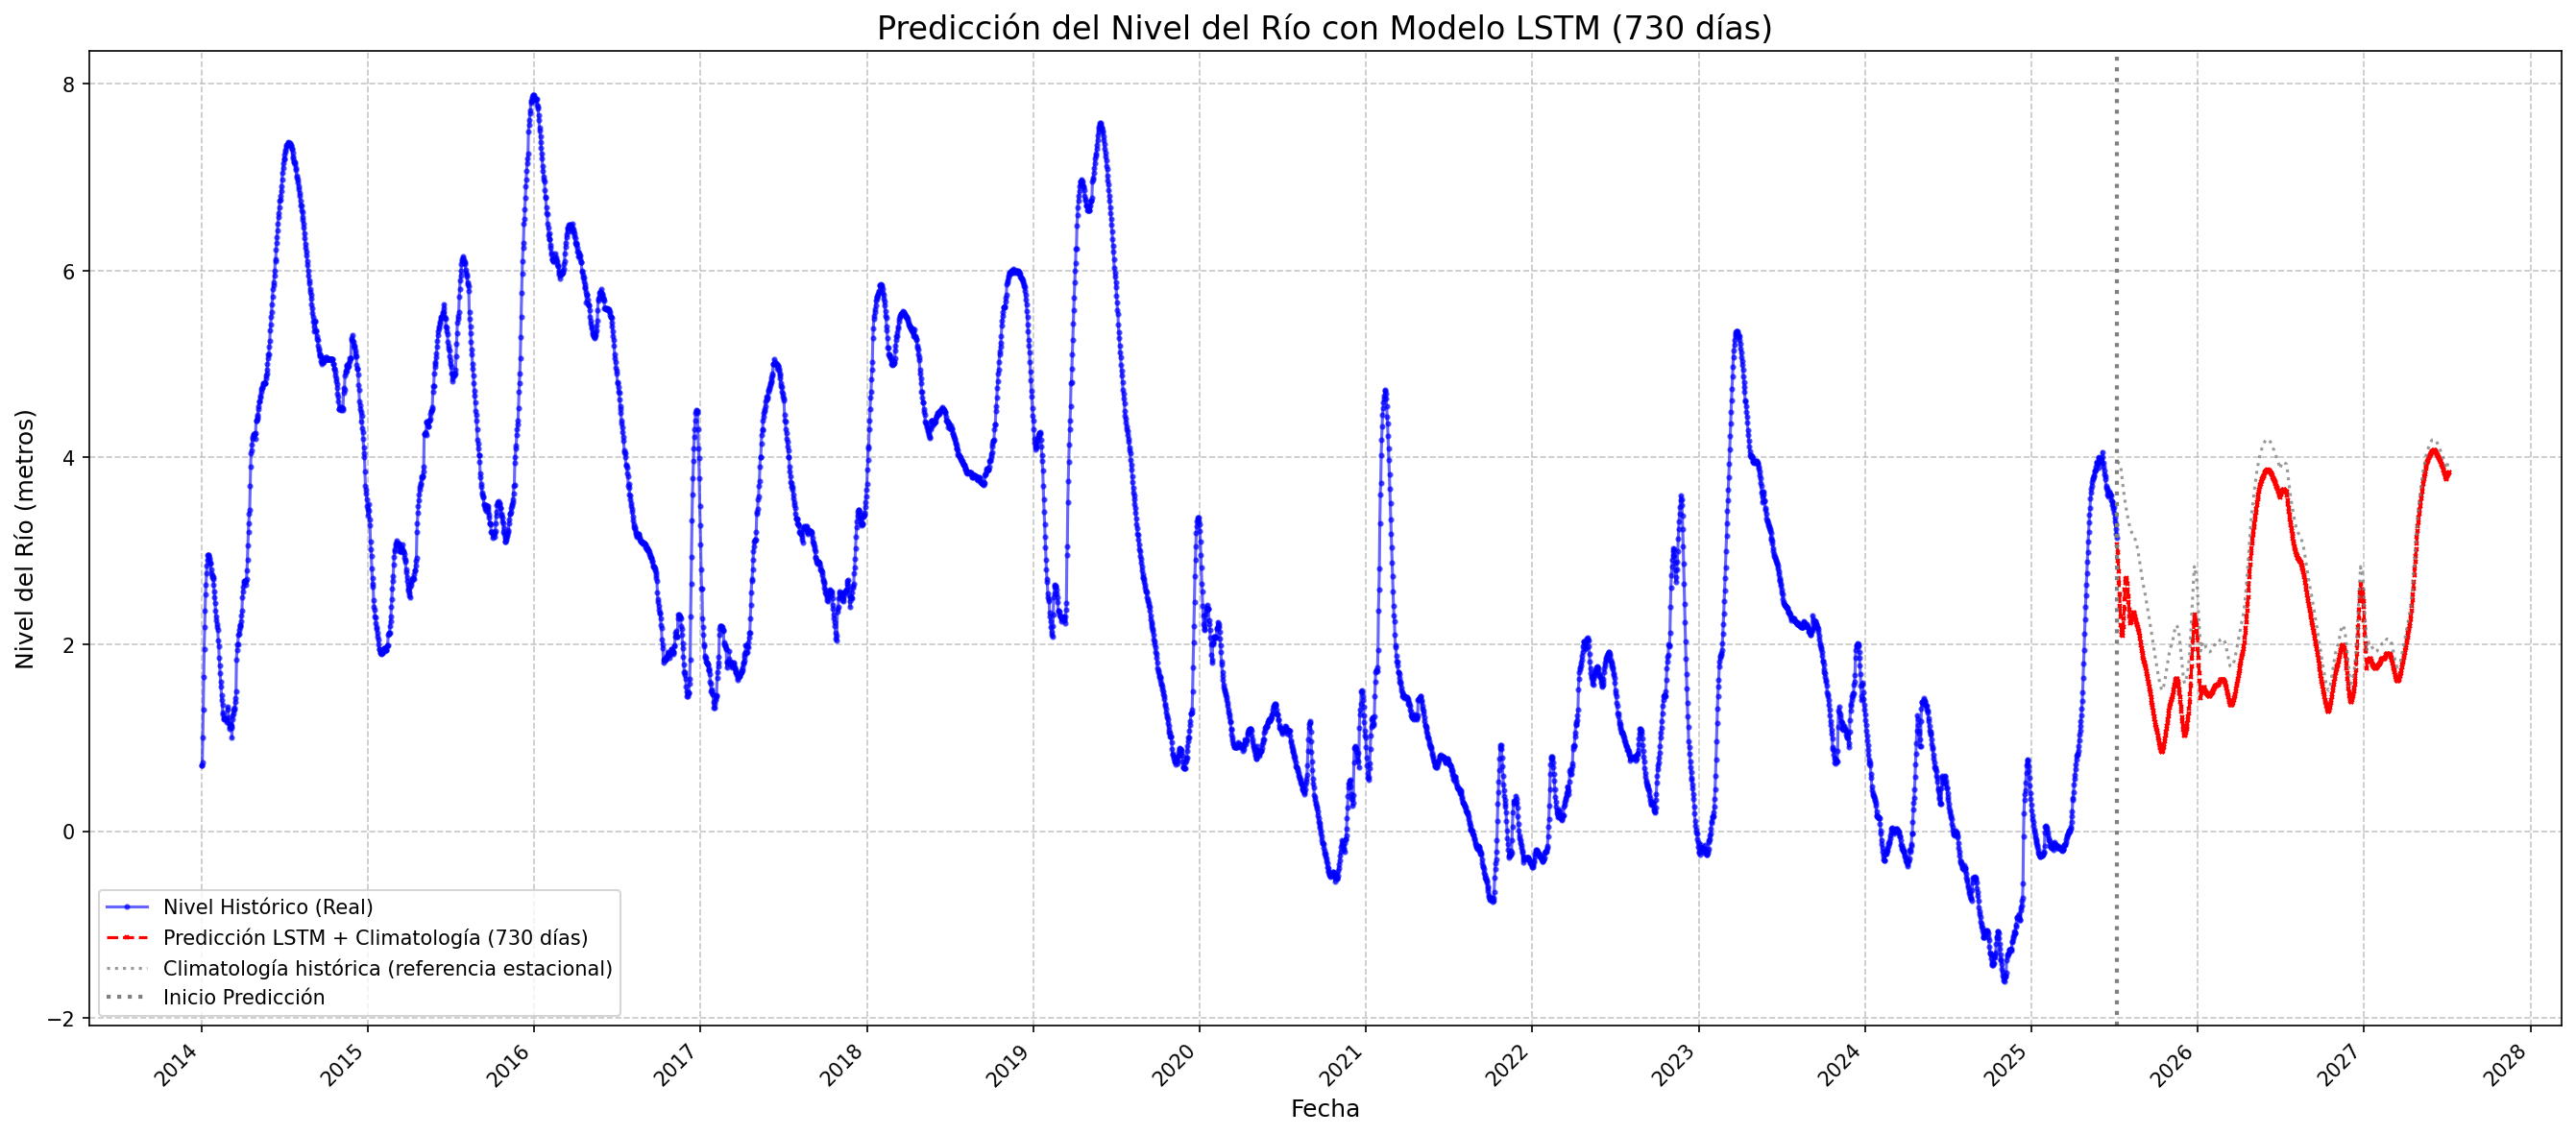
\includegraphics[width=\textwidth]{predicciones/prediccion_nivel_rio/resultados/grafico_08_historico_mas_prediccion.png}
    \caption{Serie histórica del nivel del río Paraguay y predicción LSTM a 730 días (julio 2025 -- julio 2027).}
    \label{fig:historico_prediccion}
\end{figure}

\justify
La Figura \ref{fig:zoom_transicion} muestra en detalle la transición entre datos reales (últimos 6 meses, en azul) y el inicio de la predicción (primeros 6 meses proyectados, en rojo). A partir del 8 de julio de 2025, el modelo proyecta un descenso progresivo desde los 3,08 m iniciales hasta un mínimo de aproximadamente 0,88 m hacia mediados de octubre de 2025, seguido de una recuperación que alcanza los 2,31 m hacia fines de diciembre de 2025, patrón consistente con el ciclo estacional del río.

\begin{figure}[H]
    \centering
    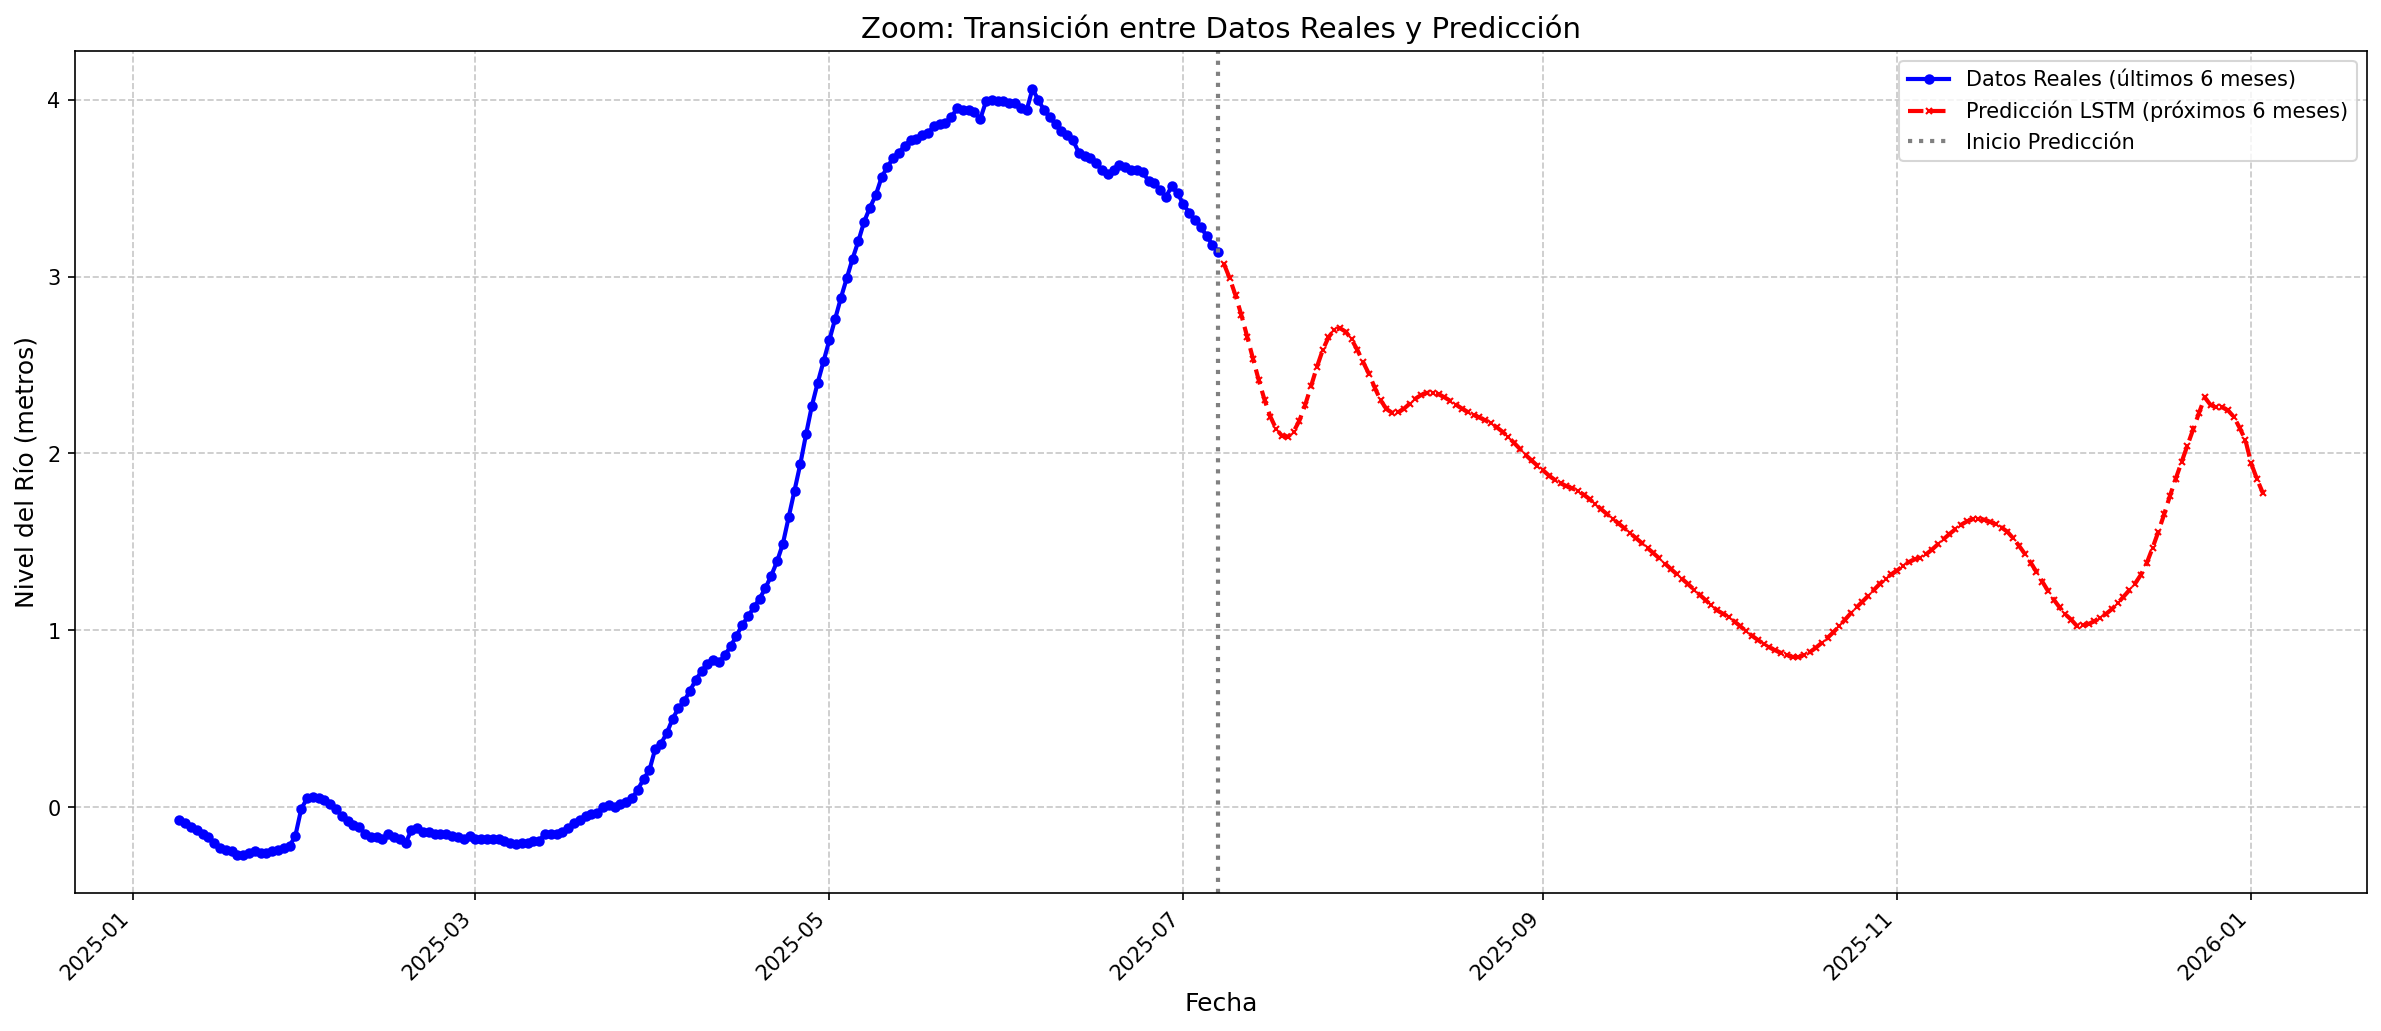
\includegraphics[width=\textwidth]{predicciones/prediccion_nivel_rio/resultados/grafico_09_zoom_transicion.png}
    \caption{Zoom en la transición entre datos reales y predicción LSTM: últimos 6 meses reales y primeros 6 meses proyectados.}
    \label{fig:zoom_transicion}
\end{figure}

\justify
La Figura \ref{fig:climatologia_prediccion} compara la predicción a 730 días con la climatología histórica tanto en la vista temporal de la proyección como en el ciclo estacional anual suavizado.

\begin{figure}[H]
    \centering
    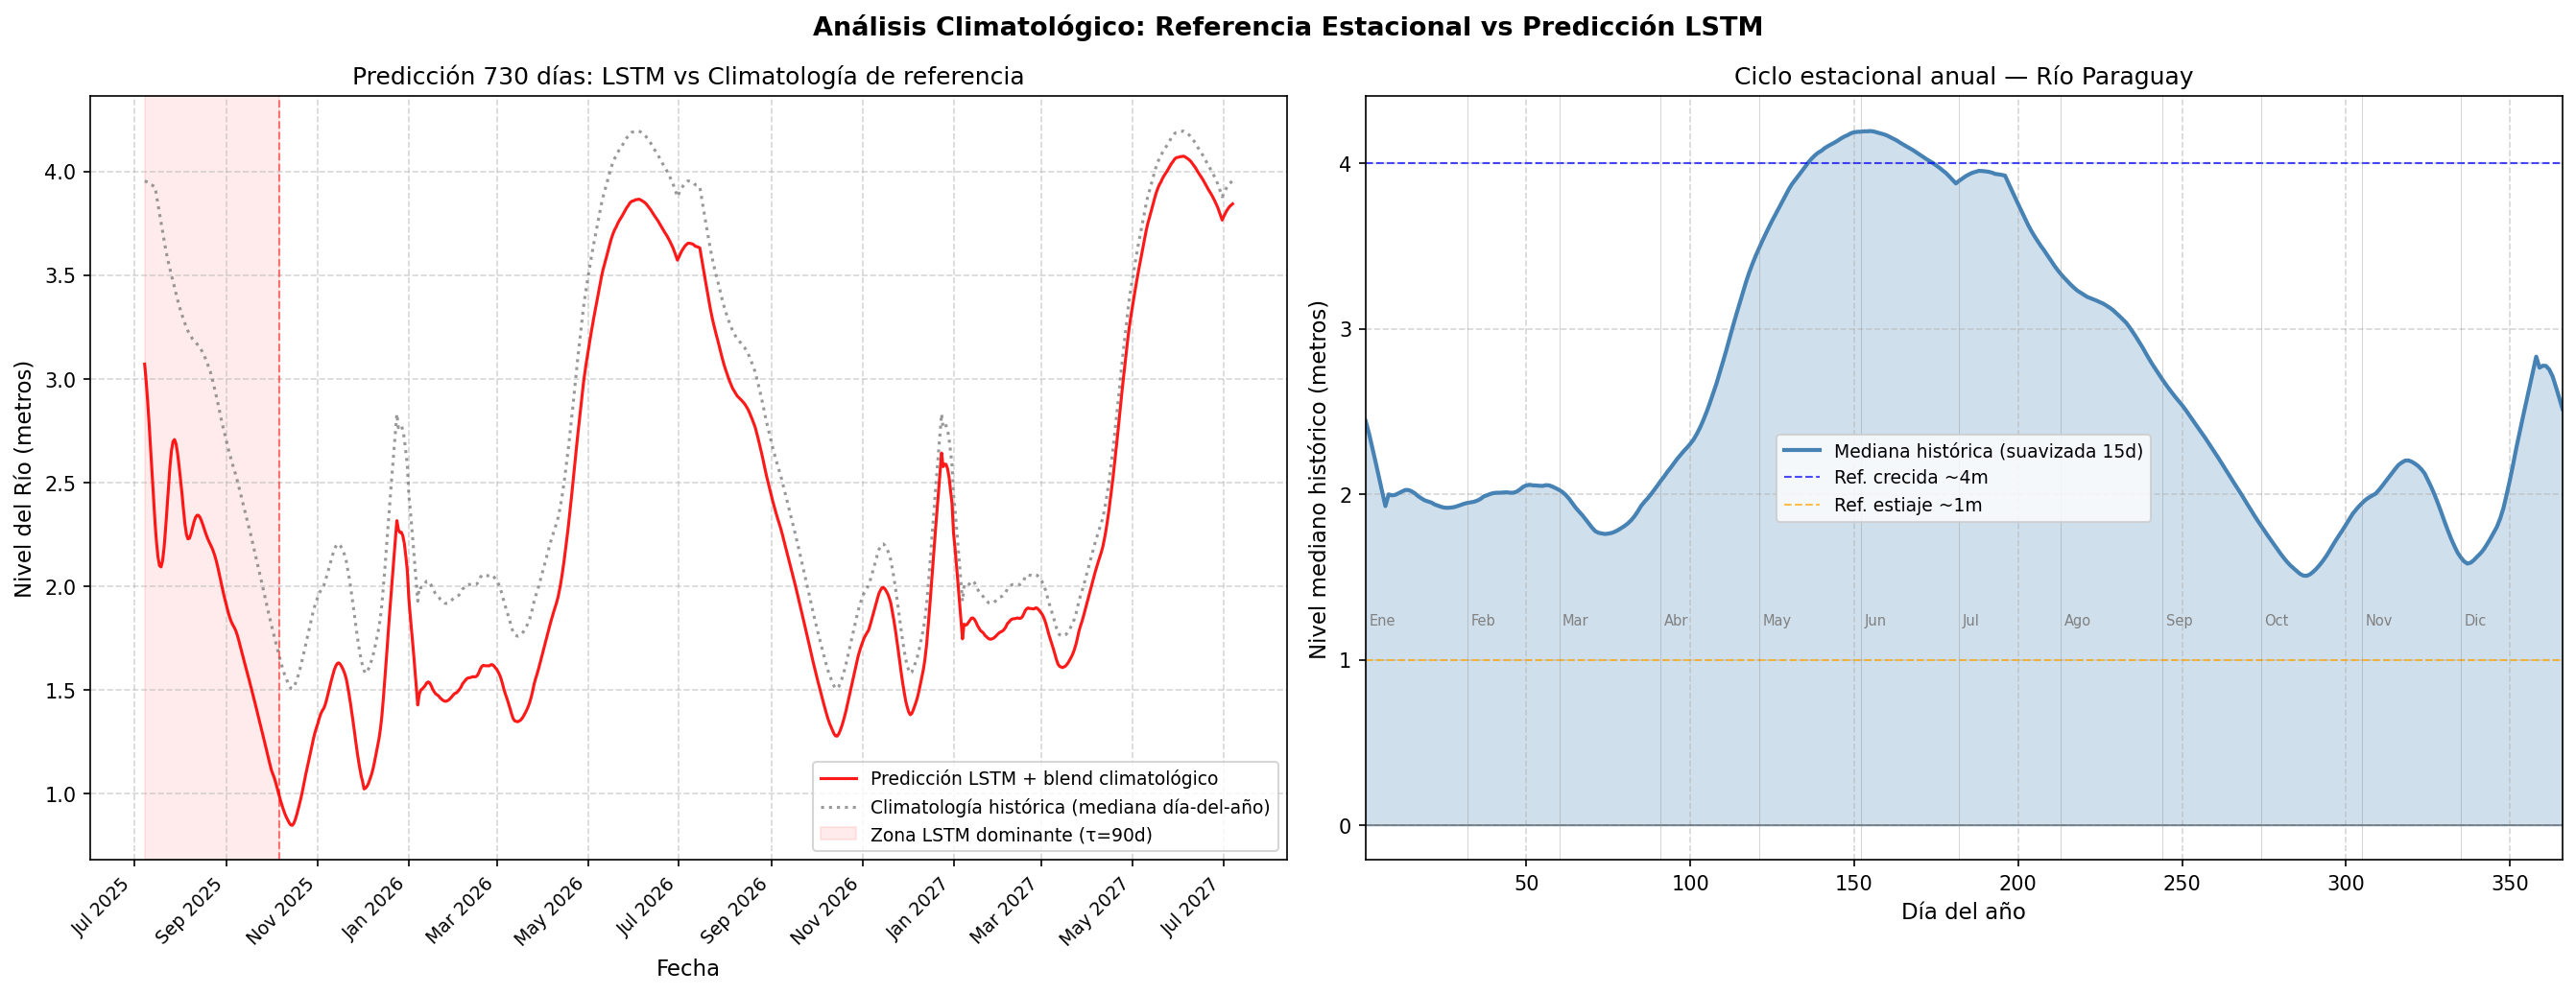
\includegraphics[width=\textwidth]{predicciones/prediccion_nivel_rio/resultados/grafico_11_climatologia_prediccion.png}
    \caption{Comparación entre la predicción LSTM a 730 días y la climatología histórica de referencia estacional.}
    \label{fig:climatologia_prediccion}
\end{figure}

\justify
La predicción a 730 días presenta un mínimo de 0,88 m, un máximo de 4,07 m, una media de 2,27 m y una desviación estándar de 0,90 m. El patrón estacional se reproduce en ambos años proyectados, con crecidas hacia los meses de mayo a julio y estiajes entre septiembre y noviembre. La amplitud de oscilación es algo menor que la de la climatología histórica, lo cual es esperable dado el blending progresivo con la climatología y la acumulación de incertidumbre en horizontes extendidos. Estos resultados validan la utilidad del modelo para estimar la variable exógena requerida por los modelos de predicción de precios de materiales de construcción.

\section{Predicción de los Precios del Cemento y del Ladrillo Común con Seasonal Autoregressive Integrated Moving Average with Exogenous Variables (SARIMAX)}
\vspace{0.3cm}
\justify
En esta sección se presentan los resultados de la aplicación del modelo SARIMAX (\textit{Seasonal AutoRegressive Integrated Moving Average with eXogenous inputs}) a la predicción de los precios de dos materiales de construcción: el cemento y el ladrillo común. El SARIMAX, implementado con \texttt{statsmodels}, ofrece un marco interpretable y con supuestos explícitos para la modelación de series temporales con componentes estacionales y variables exógenas. Para ambos materiales, se utilizaron como variables exógenas el nivel promedio mensual del río Paraguay (\texttt{Nivel\_Rio}), obtenido de las predicciones del modelo LSTM descrito en la sección anterior, y una variable binaria de cuarentena (\texttt{Cuarentena}) que captura el efecto de la pandemia de COVID-19. Los resultados abarcan el análisis exploratorio de cada serie, la selección y evaluación de cada modelo, y la generación de pronósticos a 24 meses bajo escenarios con y sin efecto pandémico.

% ============================================================
\subsection{Predicción del Precio del Cemento}
\vspace{0.3cm}
\justify
Con la proyección del nivel del río disponible, el siguiente paso fue modelar directamente el precio del cemento. El SARIMAX ofrece un marco interpretable y con supuestos explícitos; los resultados que se presentan a continuación abarcan el análisis exploratorio de la serie, la evaluación del modelo y la generación de pronósticos.

\subsubsection{Serie Histórica y Análisis Exploratorio}

\justify
La serie histórica empleada abarca registros mensuales del precio del cemento en Guaraníes (Gs.) desde enero de 2014 hasta julio de 2025, totalizando 139 observaciones. La variable endógena es el precio del cemento (\texttt{Precio\_Cemento}), mientras que las variables exógenas incorporadas son el nivel promedio mensual del río Paraguay (\texttt{Nivel\_Rio}), obtenido a partir de las predicciones del modelo LSTM descrito en la sección anterior, y una variable binaria de cuarentena (\texttt{Cuarentena}) que captura el efecto de la pandemia de COVID-19. Los estadísticos descriptivos de la serie son: precio mínimo de Gs.~48.000, precio máximo de Gs.~76.036, precio promedio de Gs.~53.872 y desviación estándar de Gs.~7.460.

\begin{figure}[ht]
    \centering
    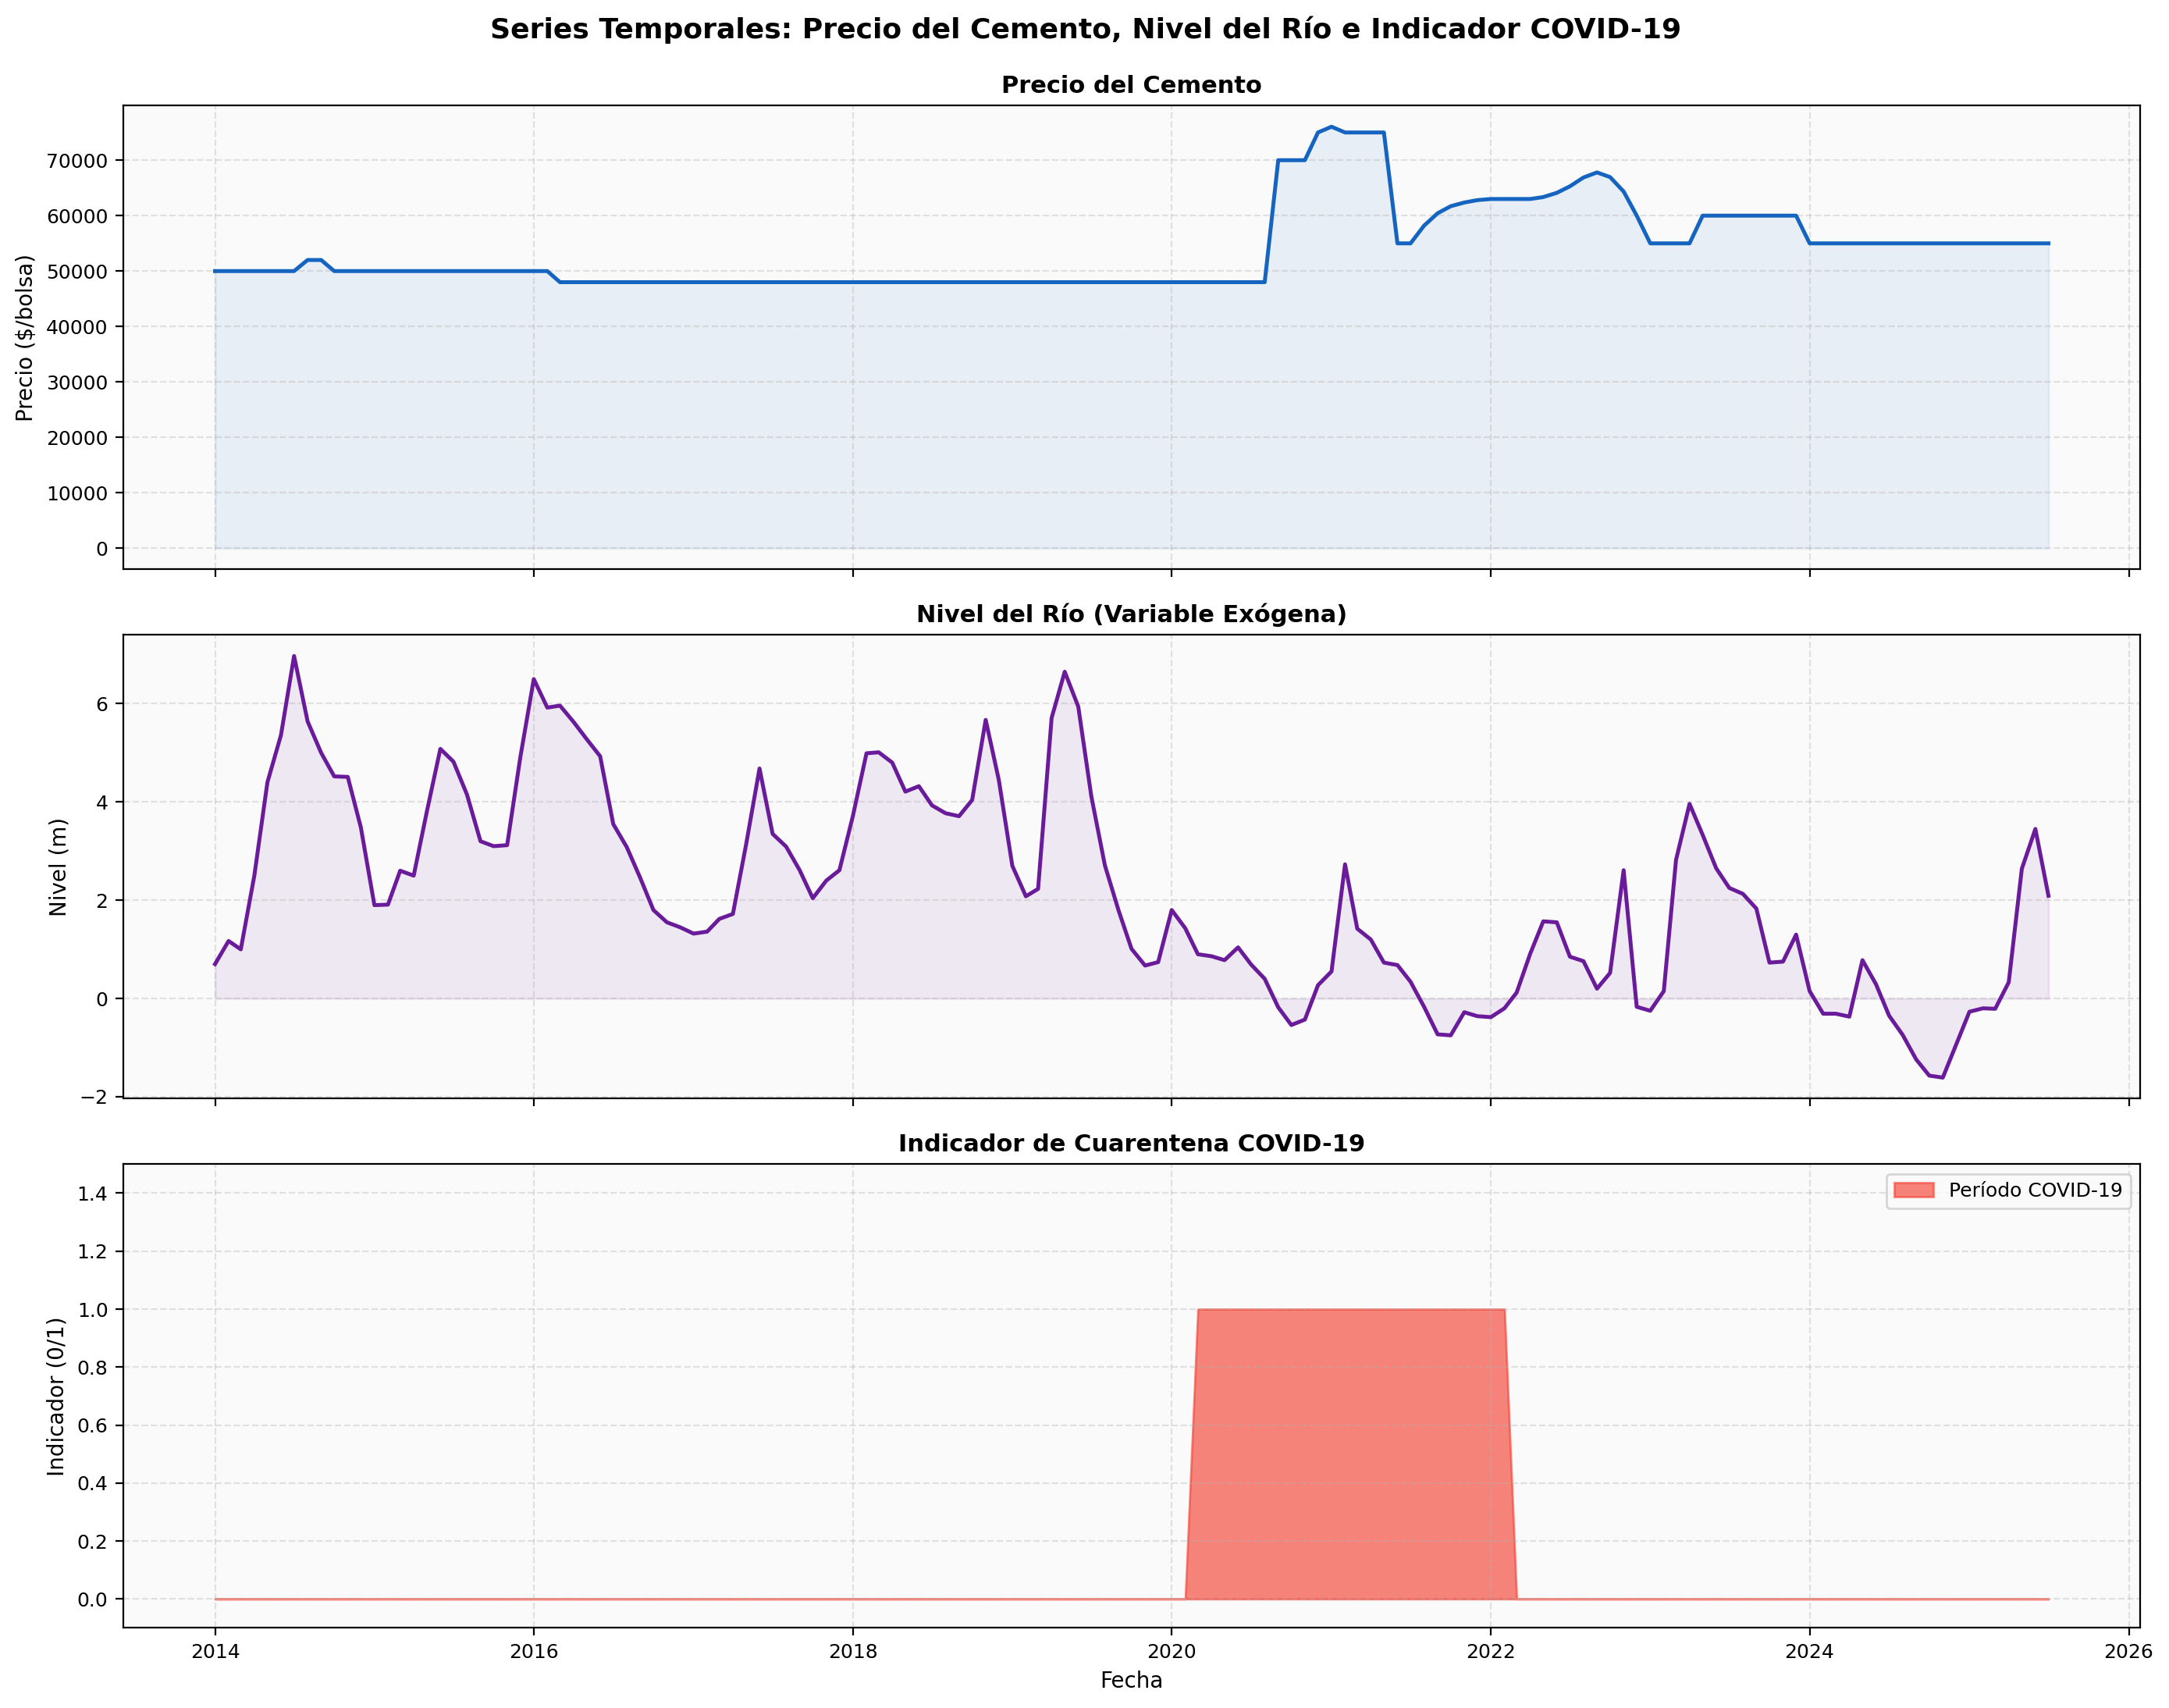
\includegraphics[width=\textwidth]{predicciones/prediccion_sarimax_cemento/graficos/01_series_temporales.png}
    \caption{Series temporales del precio mensual del cemento (Gs.) y del nivel del río Paraguay (m), período 2014--2025.}
    \label{fig:sarimax_series}
\end{figure}

\justify
La Figura \ref{fig:sarimax_series} muestra la evolución conjunta del precio del cemento y del nivel del río Paraguay. Se aprecia una tendencia ascendente sostenida en el precio del cemento a lo largo del período analizado, con una aceleración marcada a partir de 2020 que coincide con el período de pandemia y las disrupciones en la cadena de suministros. El nivel del río, por su parte, presenta la variabilidad estacional interanual característica, con ciclos de crecida y estiaje que constituyen la variable exógena hidrológica del modelo.

\begin{figure}[ht]
    \centering
    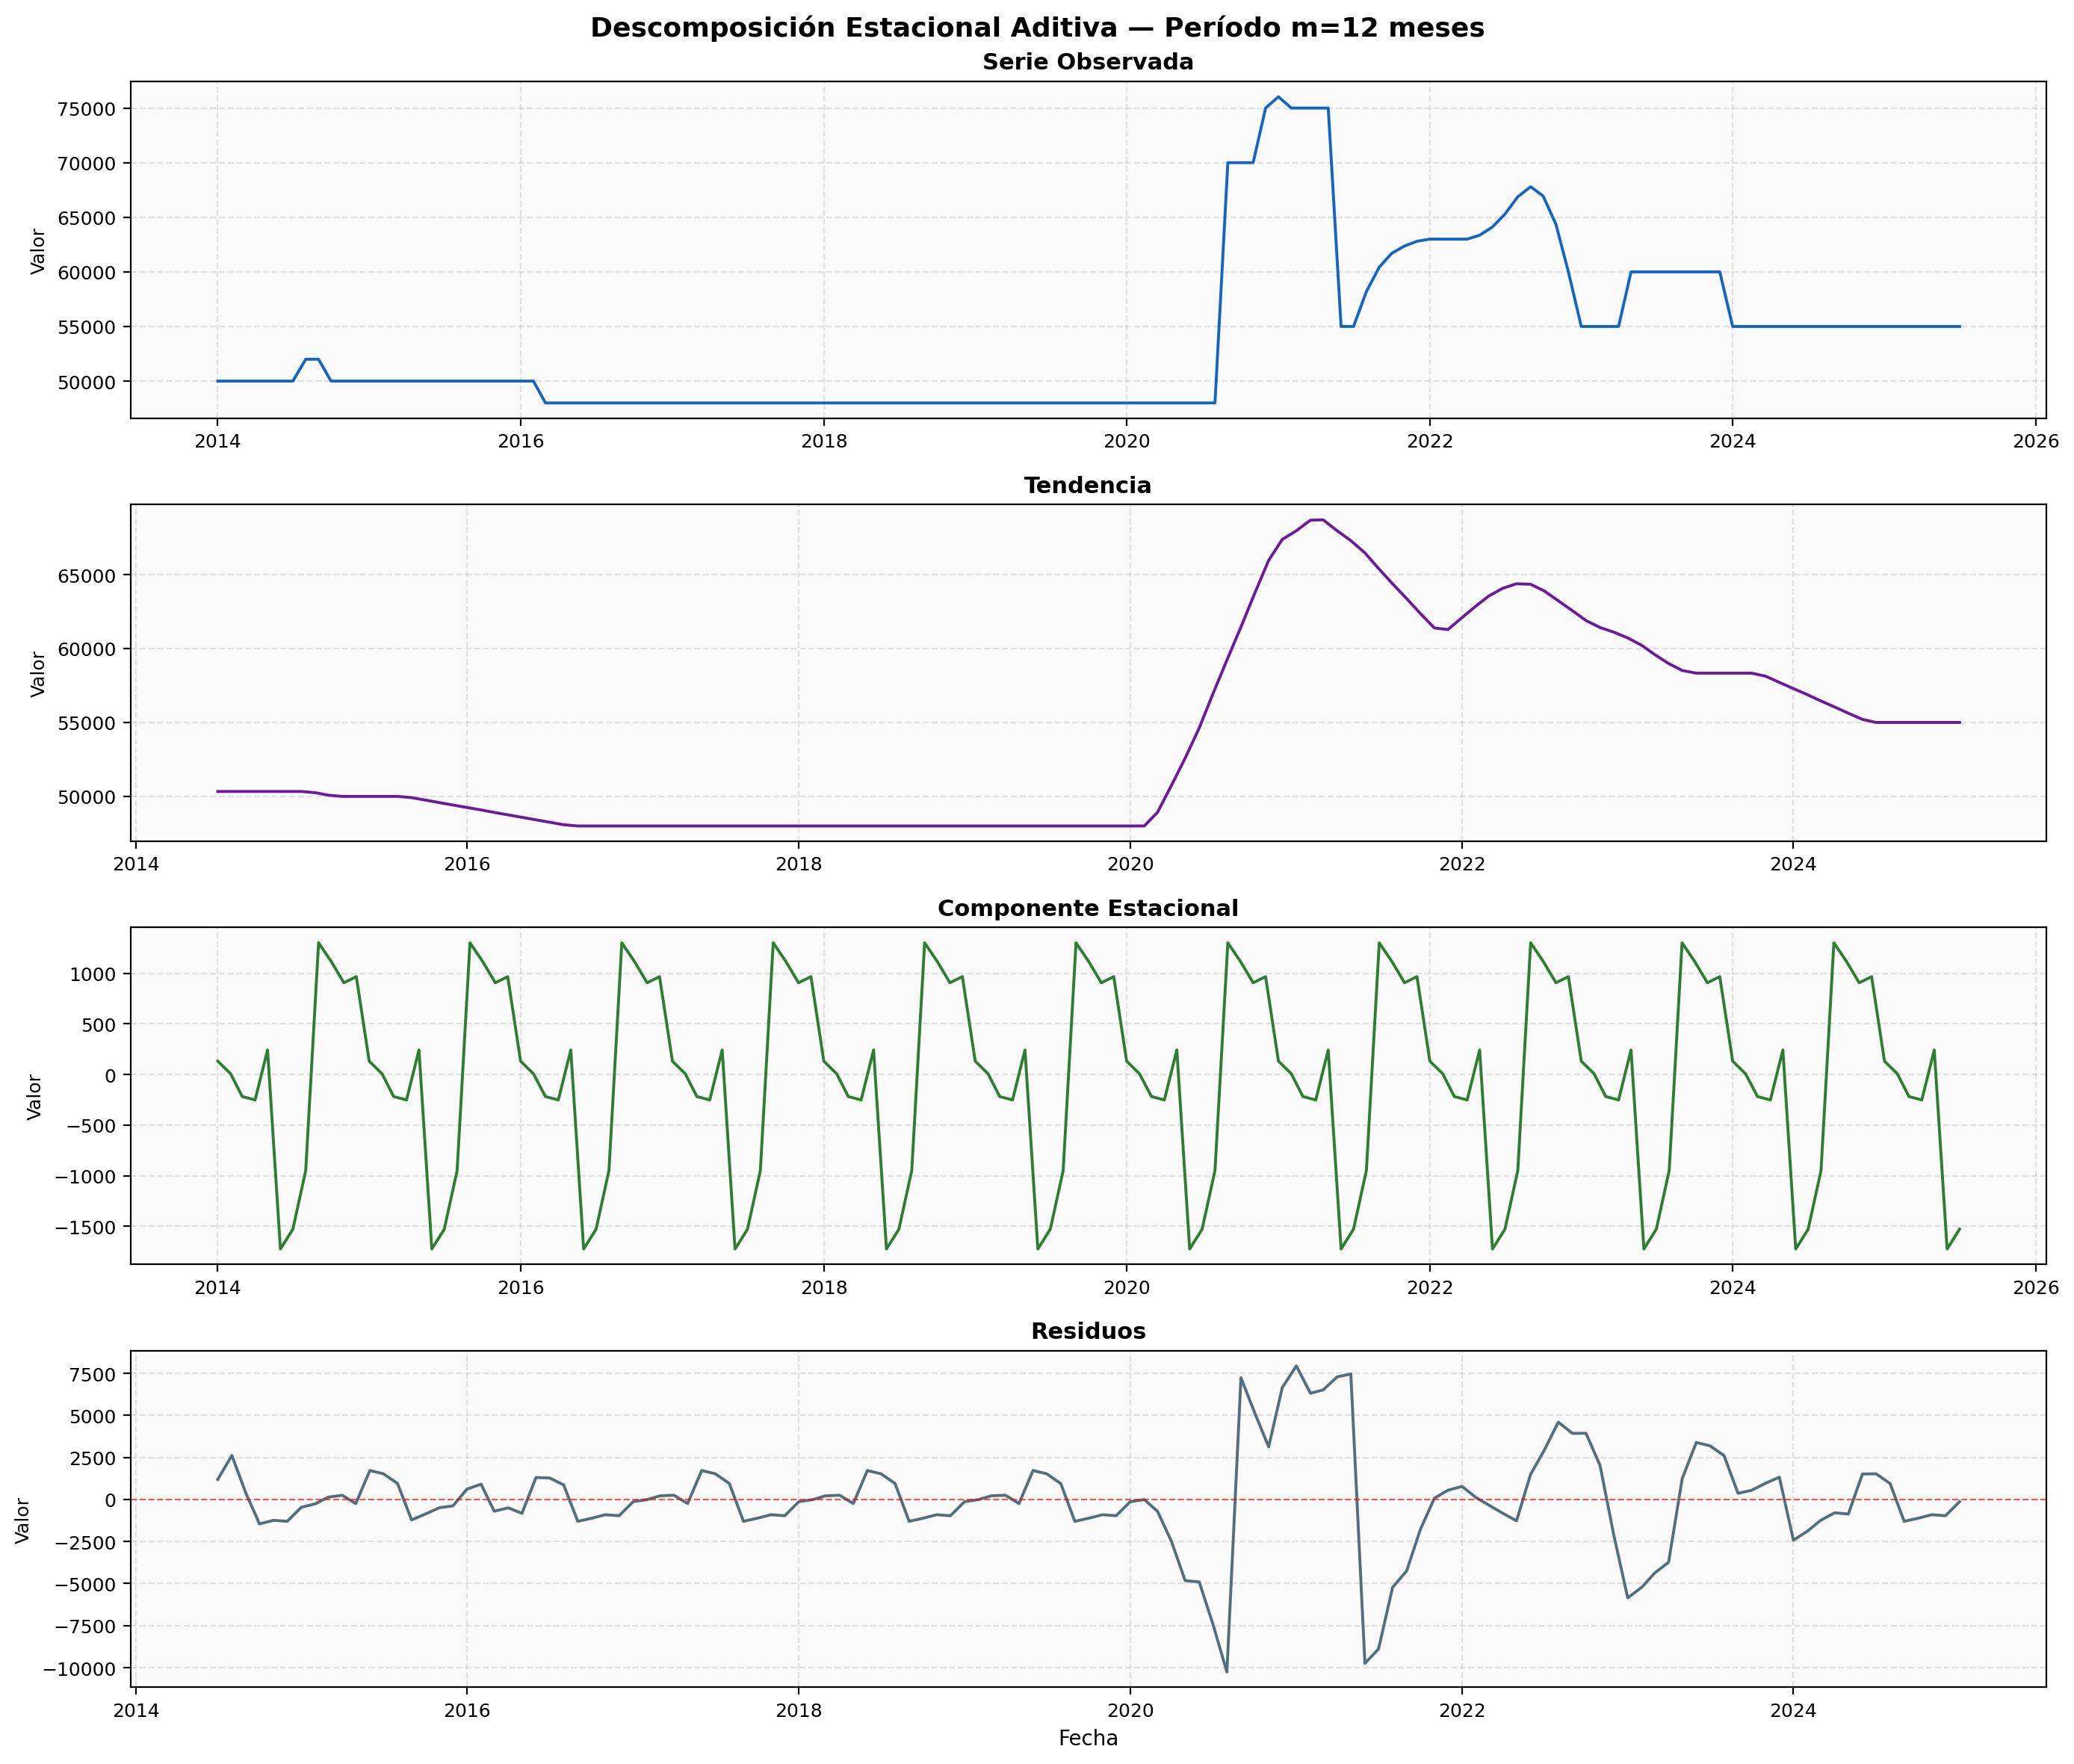
\includegraphics[width=\textwidth]{predicciones/prediccion_sarimax_cemento/graficos/02_descomposicion_estacional.png}
    \caption{Descomposición estacional de la serie de precio del cemento: tendencia, estacionalidad y componente residual.}
    \label{fig:sarimax_descomposicion}
\end{figure}

\justify
La Figura \ref{fig:sarimax_descomposicion} presenta la descomposición clásica de la serie en sus componentes de tendencia, estacionalidad y residuo. La componente de tendencia confirma el crecimiento sostenido del precio, en particular el salto registrado entre 2020 y 2022. La componente estacional revela patrones de amplitud moderada con período anual, mientras que los residuos no evidencian estructura sistemática evidente, lo que sugiere la adecuación de la descomposición.

\begin{figure}[ht]
    \centering
    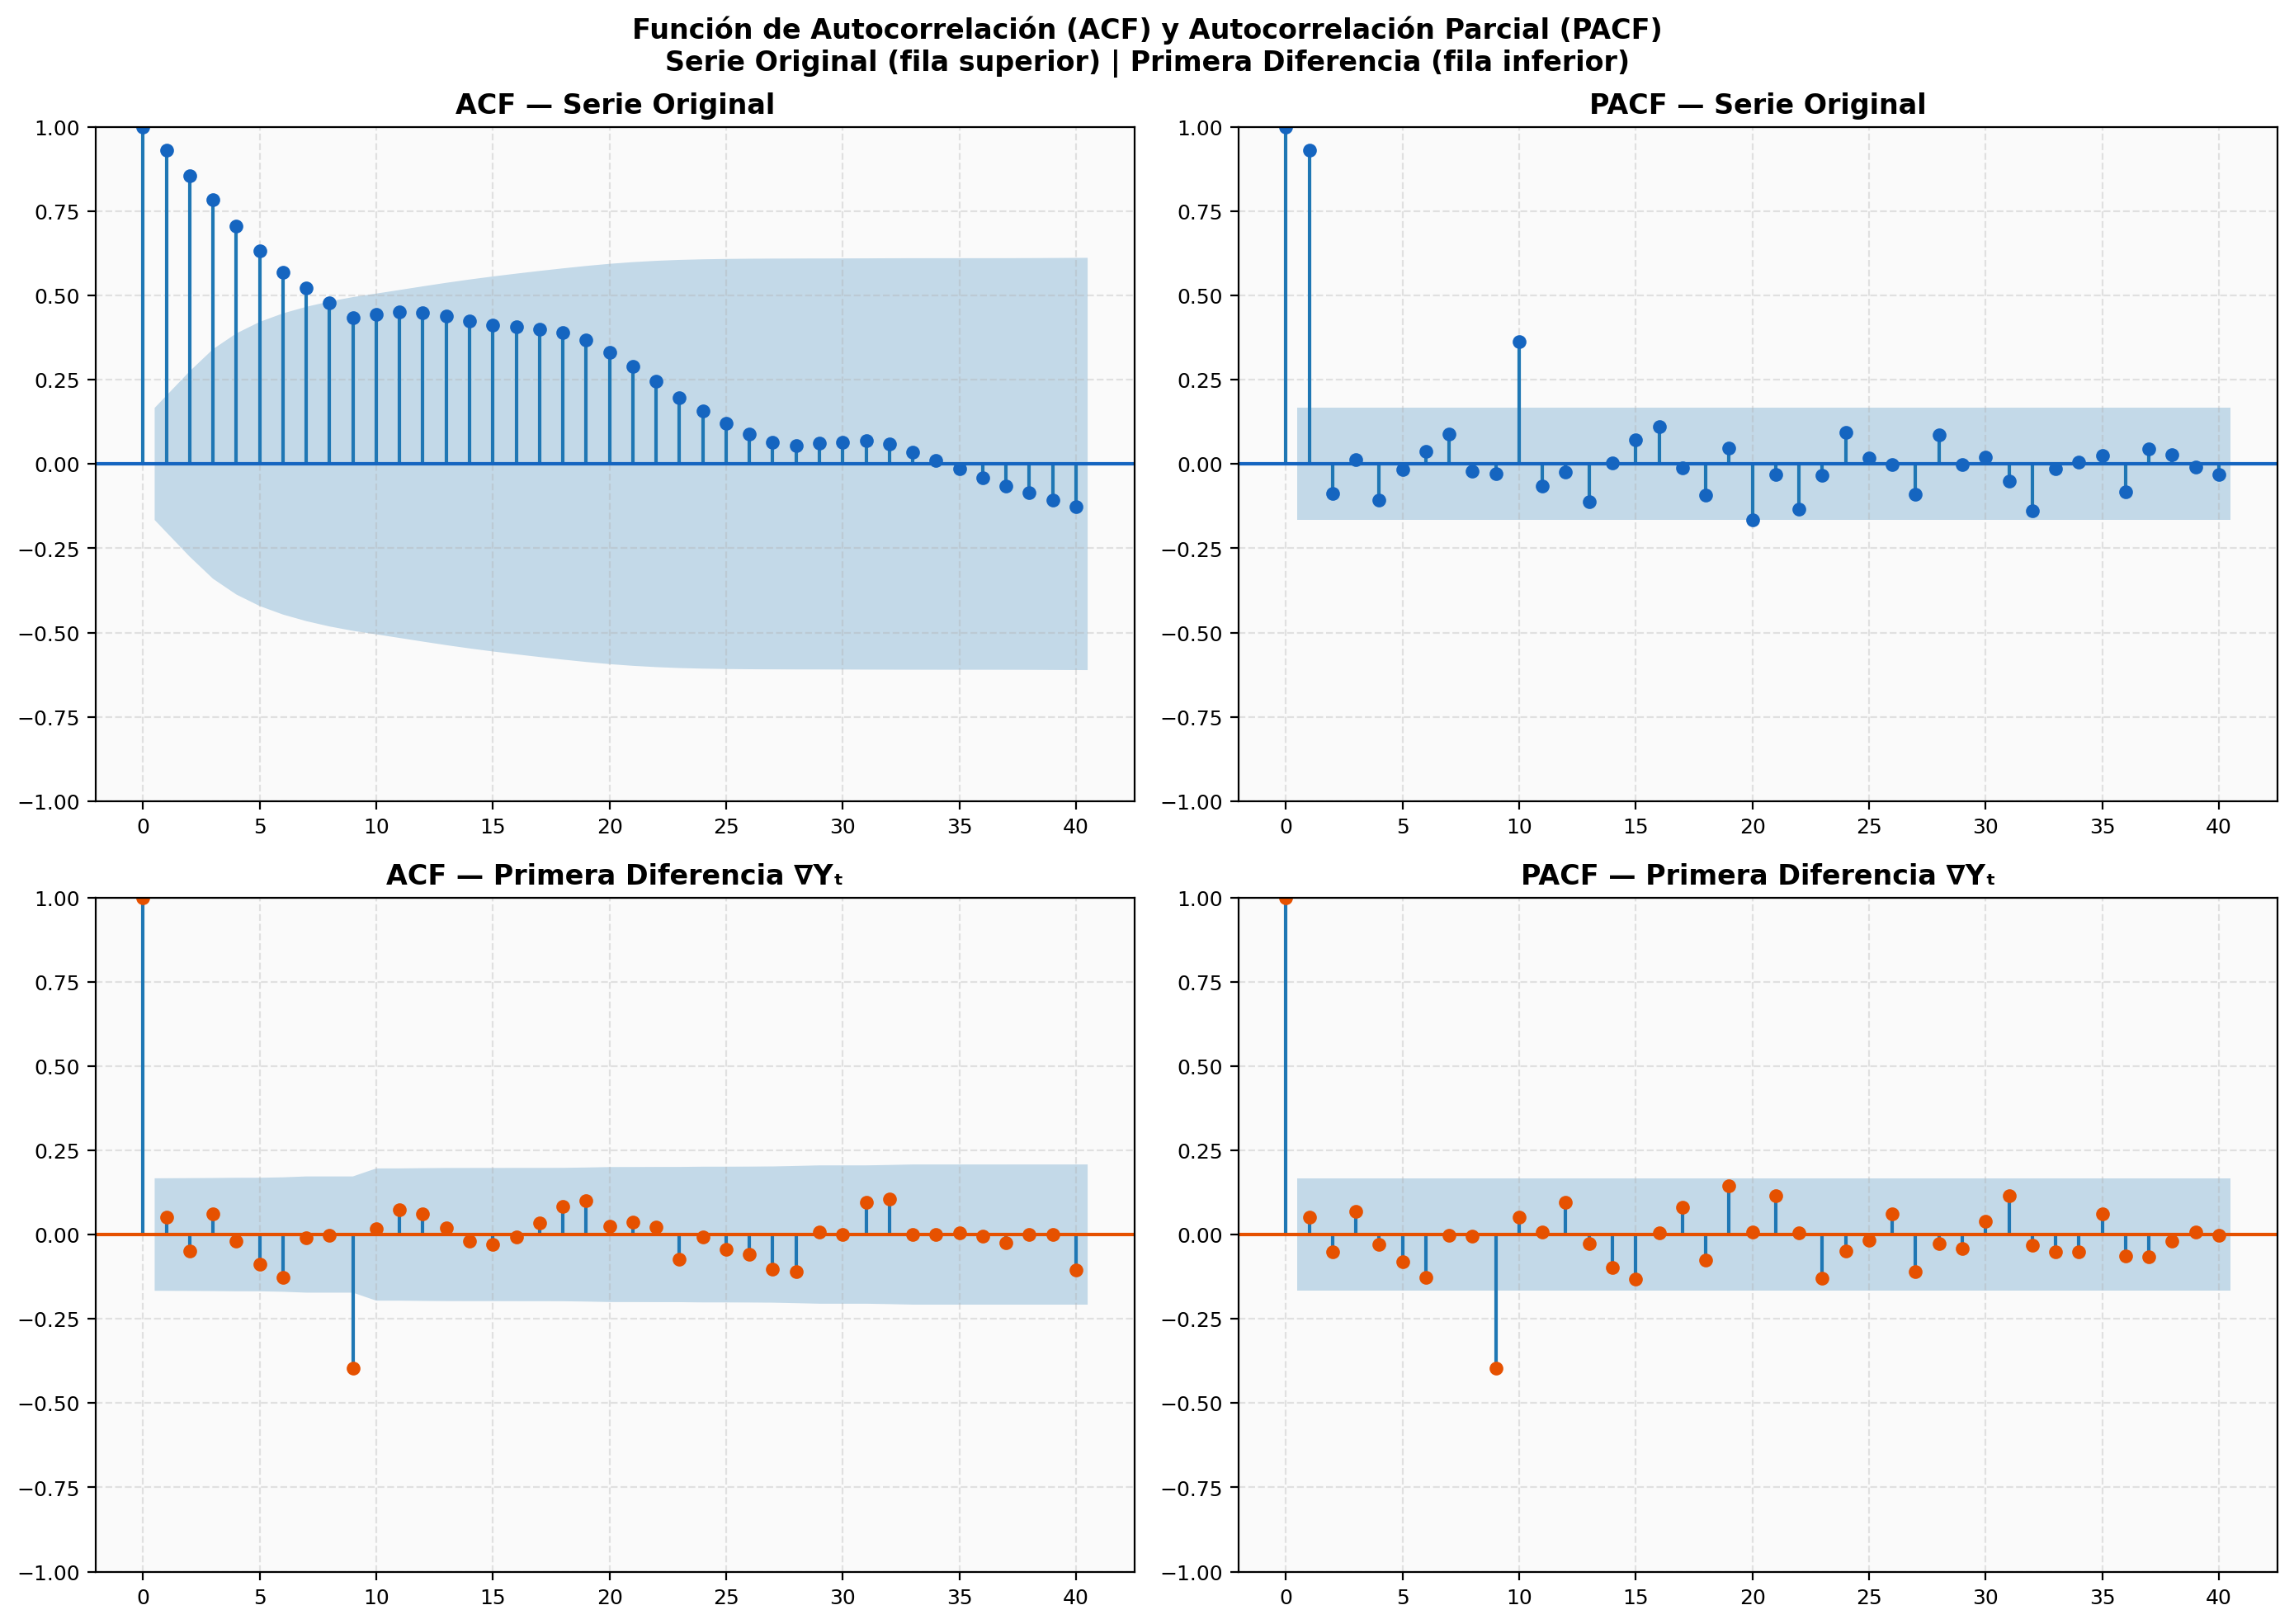
\includegraphics[width=\textwidth]{predicciones/prediccion_sarimax_cemento/graficos/03_acf_pacf.png}
    \caption{Funciones de autocorrelación (ACF) y autocorrelación parcial (PACF) de la serie del precio del cemento en niveles y en primeras diferencias.}
    \label{fig:sarimax_acf_pacf}
\end{figure}

\justify
La Figura \ref{fig:sarimax_acf_pacf} muestra las funciones ACF y PACF de la serie original y de su primera diferencia. La serie en niveles presenta una ACF con decaimiento lento, característico de procesos no estacionarios integrados. Tras aplicar la primera diferencia, la ACF decae abruptamente hacia cero a partir del primer rezago, lo que indica que la serie diferenciada es estacionaria. Este diagnóstico justifica el orden de integración $d=1$ adoptado en el modelo SARIMAX.

\begin{figure}[ht]
    \centering
    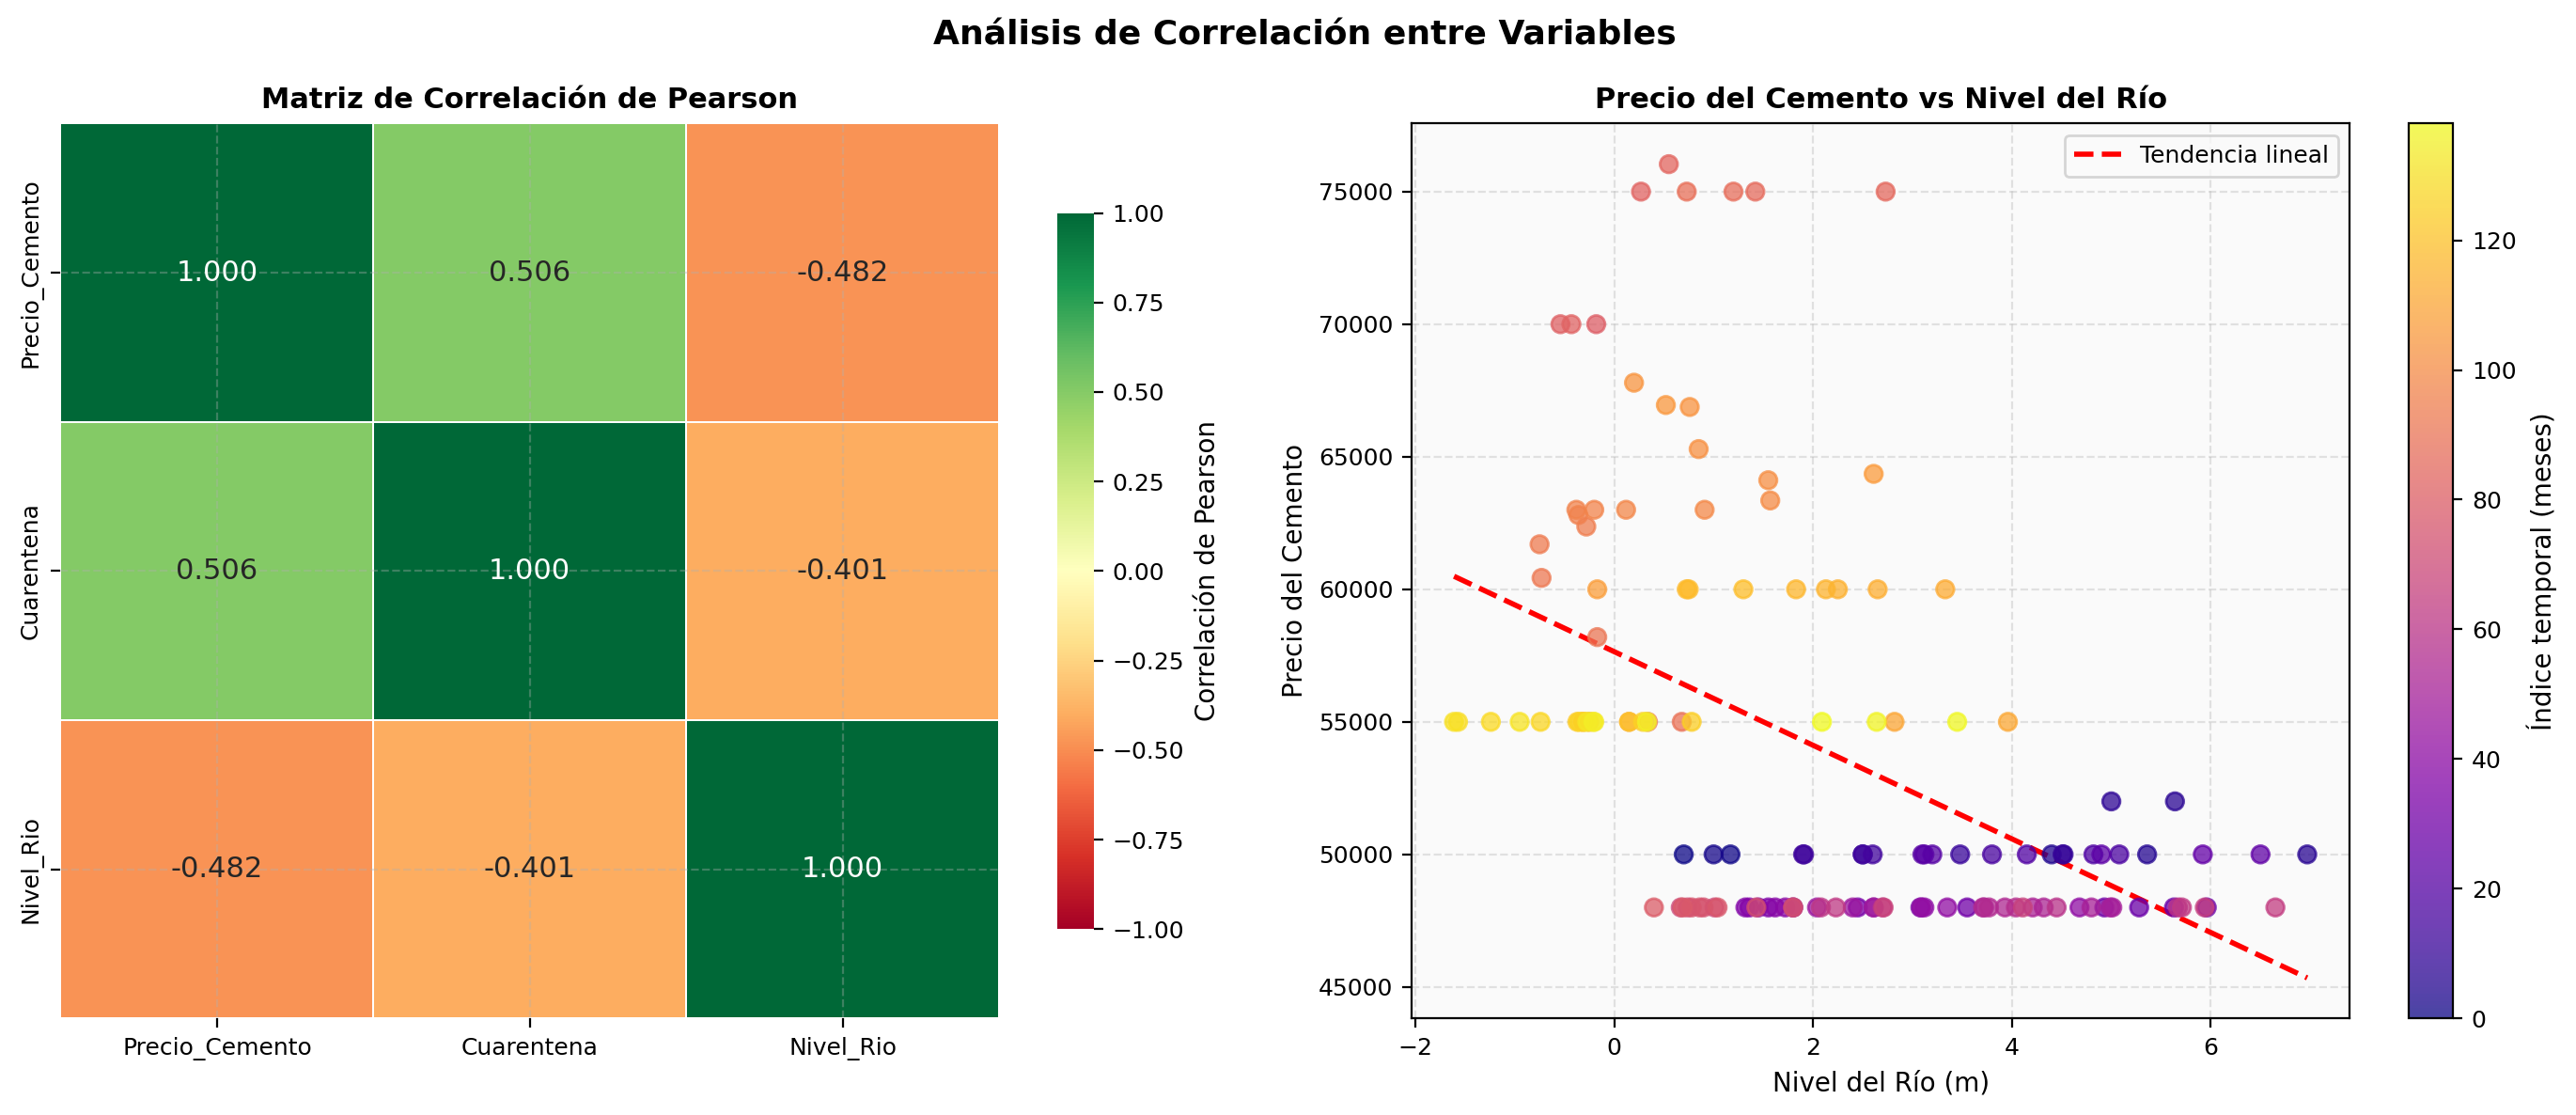
\includegraphics[width=0.8\textwidth]{predicciones/prediccion_sarimax_cemento/graficos/04_correlacion.png}
    \caption{Matriz de correlación entre el precio del cemento, el nivel del río Paraguay y la variable de cuarentena.}
    \label{fig:sarimax_correlacion}
\end{figure}

\justify
La Figura \ref{fig:sarimax_correlacion} presenta la matriz de correlación entre las variables del modelo. La correlación entre el precio del cemento y el nivel del río Paraguay es de magnitud moderada y negativa, coherente con la hipótesis de que los períodos de crecida dificultan la logística de abastecimiento y presionan al alza los costos. La variable de cuarentena muestra correlación positiva con el precio, capturando el efecto inflacionario del período pandémico.

\begin{figure}[ht]
    \centering
    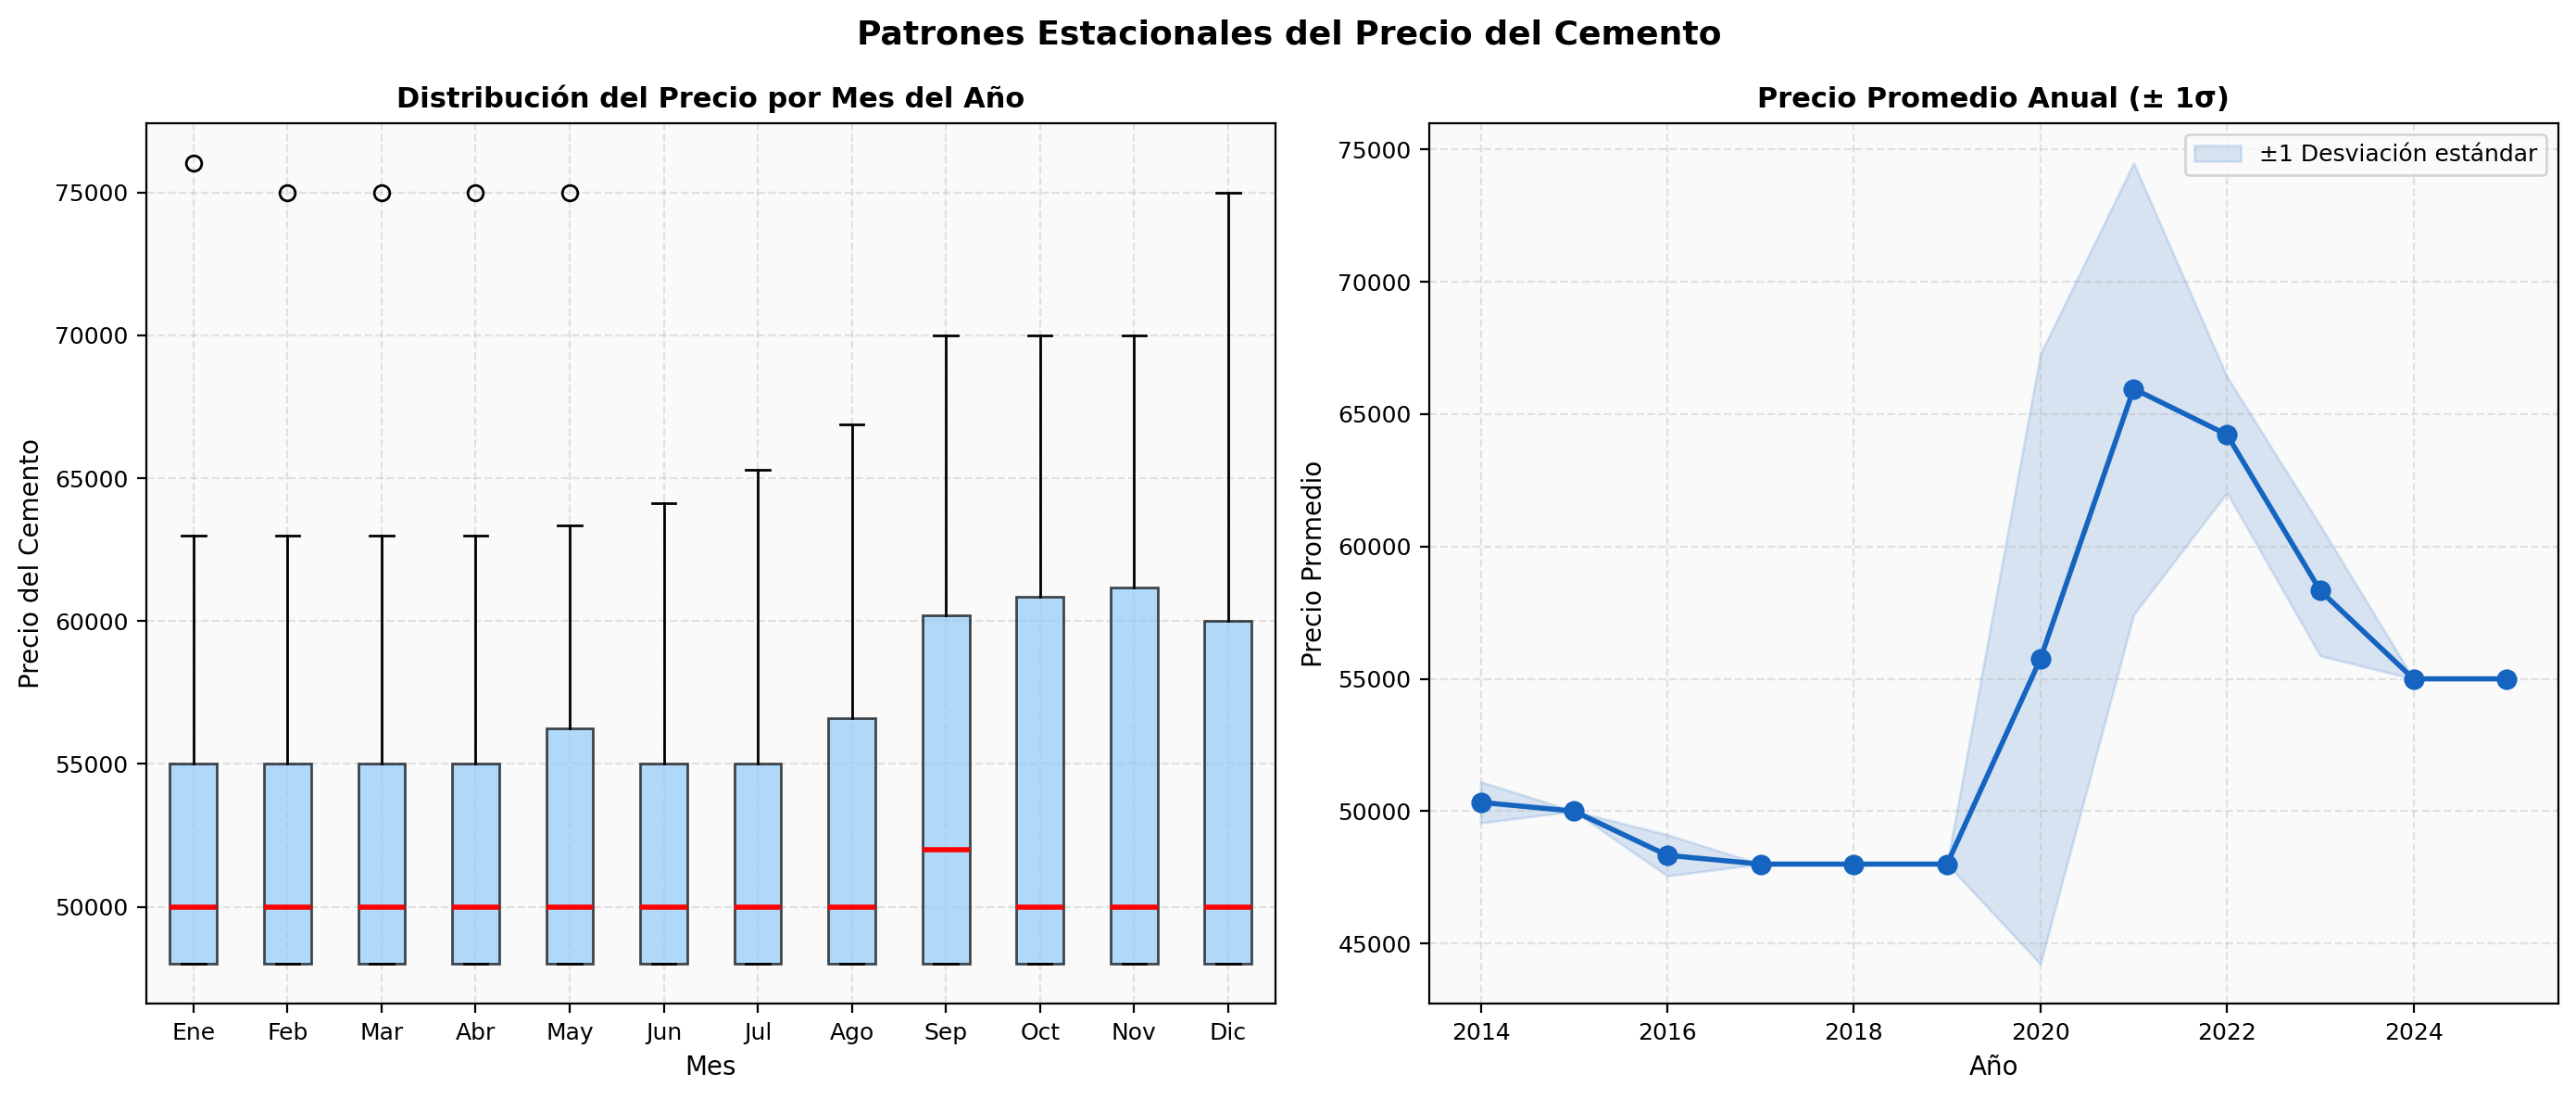
\includegraphics[width=\textwidth]{predicciones/prediccion_sarimax_cemento/graficos/05_patron_estacional.png}
    \caption{Patrón estacional del precio mensual del cemento a lo largo del año.}
    \label{fig:sarimax_estacional}
\end{figure}

\justify
La Figura \ref{fig:sarimax_estacional} ilustra el patrón estacional del precio del cemento a lo largo del ciclo anual. Se observa que los precios tienden a ser ligeramente superiores en los meses de mayor actividad de la construcción (primer y cuarto trimestre), mientras que en los meses de lluvia intensa y posibles interrupciones logísticas se registran variaciones de menor amplitud, aunque dentro de un rango de fluctuación contenido.

\subsubsection{Modelo SARIMAX: Selección y Parámetros}

\justify
La selección del orden óptimo del modelo SARIMAX se realizó mediante una búsqueda exhaustiva sobre el espacio de parámetros $(p, d, q) \times (P, D, Q)_{12}$, minimizando el Criterio de Información de Akaike (AIC). El modelo seleccionado corresponde al orden SARIMAX$(0,1,0)(0,0,0)_{12}$, equivalente a un paseo aleatorio con variables exógenas, con un AIC de 2566{,}18 y un BIC de 2574{,}94.

\justify
Los parámetros estimados del modelo se resumen en la Tabla \ref{tab:sarimax_params}. El coeficiente asociado al nivel del río (\texttt{Nivel\_Rio}) resultó negativo ($-55{,}34$~Gs./m) aunque estadísticamente no significativo ($p=0{,}895$), lo que puede atribuirse a la escasa variabilidad de esta variable en el subconjunto de ajuste o a la dominancia de la tendencia de largo plazo en la serie. La variable \texttt{Cuarentena} tampoco alcanzó significancia estadística en el marco paramétrico del modelo integrado, dado que su efecto queda parcialmente absorbido por la diferenciación de la serie.

\begin{table}[ht]
    \centering
    \caption{Parámetros estimados del modelo SARIMAX$(0,1,0)(0,0,0)_{12}$ para la predicción del precio del cemento.}
    \label{tab:sarimax_params}
    \begin{tabular}{lrrrr}
        \toprule
        \textbf{Parámetro} & \textbf{Coeficiente} & \textbf{Error est.} & \textbf{z} & \textbf{p-valor} \\
        \midrule
        \texttt{Nivel\_Rio}  & $-55{,}340$ & $418{,}862$ & $-0{,}132$ & $0{,}895$ \\
        \texttt{Cuarentena}  & $-23{,}482$ & $9{,}49 \times 10^{5}$ & $-2{,}47 \times 10^{-5}$ & $1{,}000$ \\
        $\sigma^{2}$         & $7{,}80 \times 10^{6}$ & $2{,}15 \times 10^{5}$ & $36{,}223$ & $0{,}000$ \\
        \midrule
        \multicolumn{2}{l}{AIC} & \multicolumn{3}{r}{2566{,}18} \\
        \multicolumn{2}{l}{BIC} & \multicolumn{3}{r}{2574{,}94} \\
        \multicolumn{2}{l}{Log-verosimilitud} & \multicolumn{3}{r}{$-1280{,}09$} \\
        \bottomrule
    \end{tabular}
\end{table}

\subsubsection{Modelo SARIMAX: Ajuste y Evaluación}

\begin{figure}[ht]
    \centering
    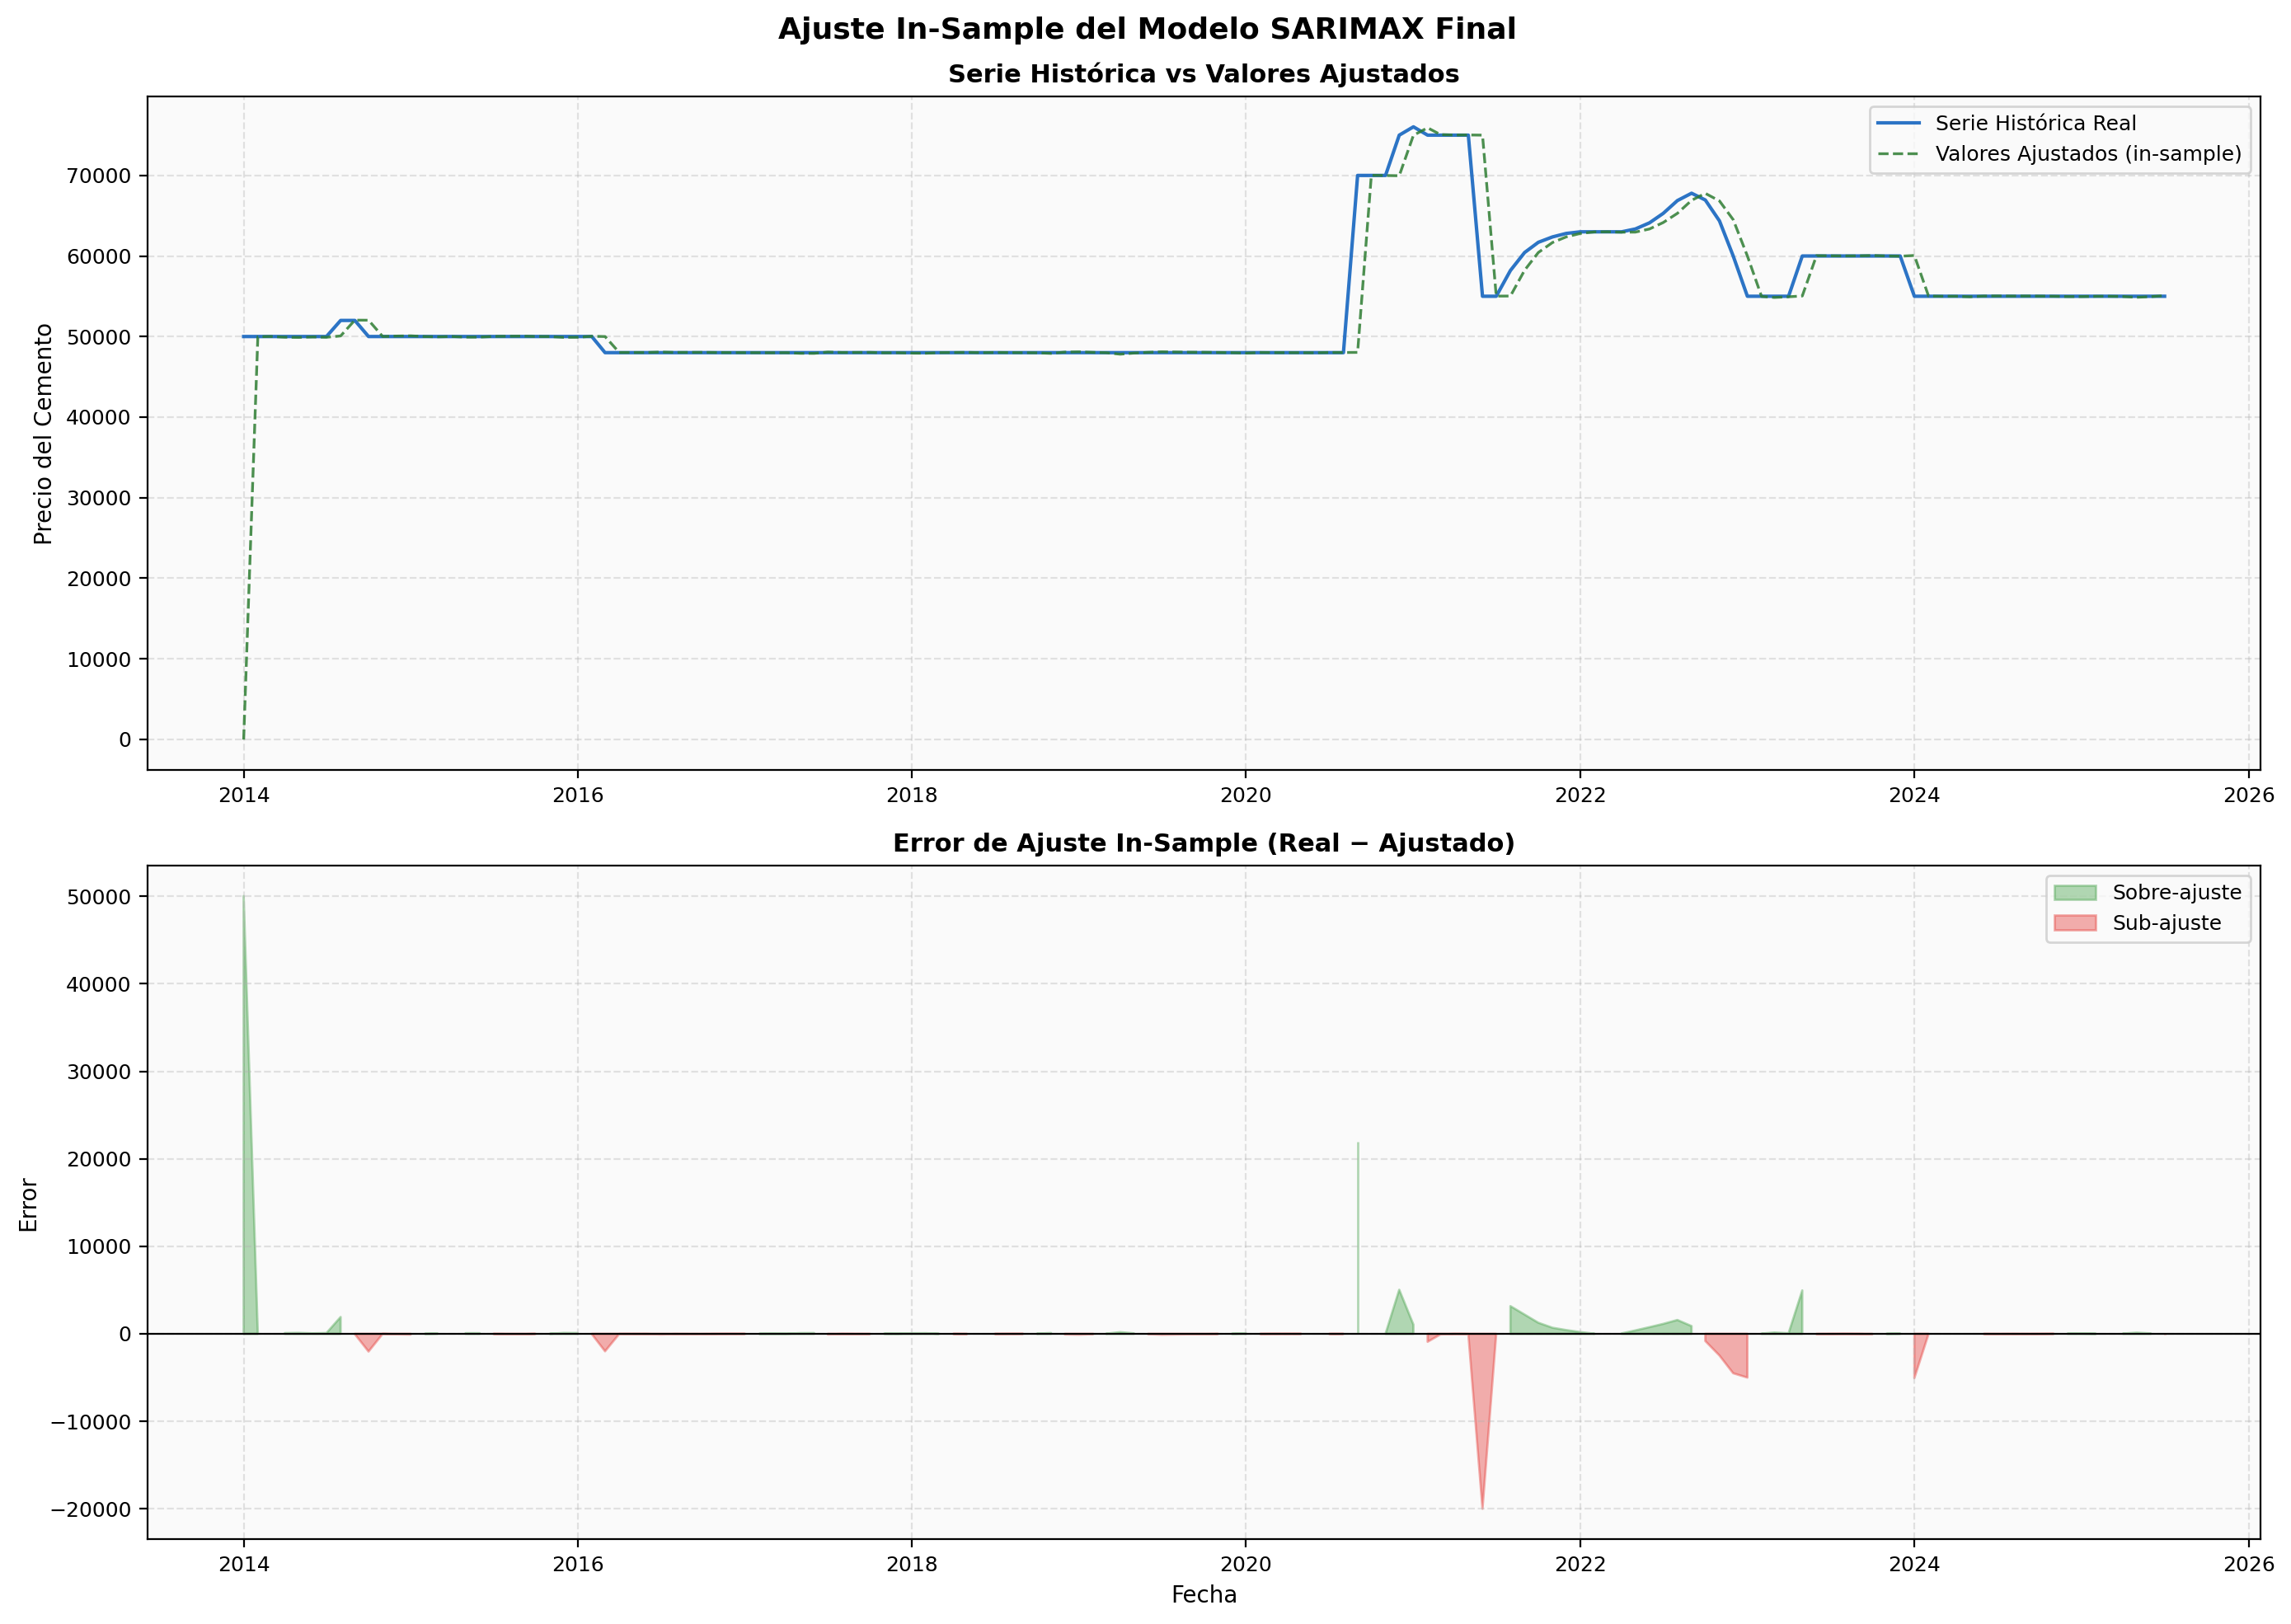
\includegraphics[width=\textwidth]{predicciones/prediccion_sarimax_cemento/graficos/11_ajuste_insample.png}
    \caption{Ajuste in-sample del modelo SARIMAX: valores reales versus valores ajustados sobre el período de entrenamiento.}
    \label{fig:sarimax_insample}
\end{figure}

\justify
La Figura \ref{fig:sarimax_insample} muestra el ajuste del modelo sobre los datos de entrenamiento. El modelo sigue con precisión la trayectoria histórica del precio del cemento, incluyendo la aceleración registrada en el período 2020--2022.

\begin{figure}[ht]
    \centering
    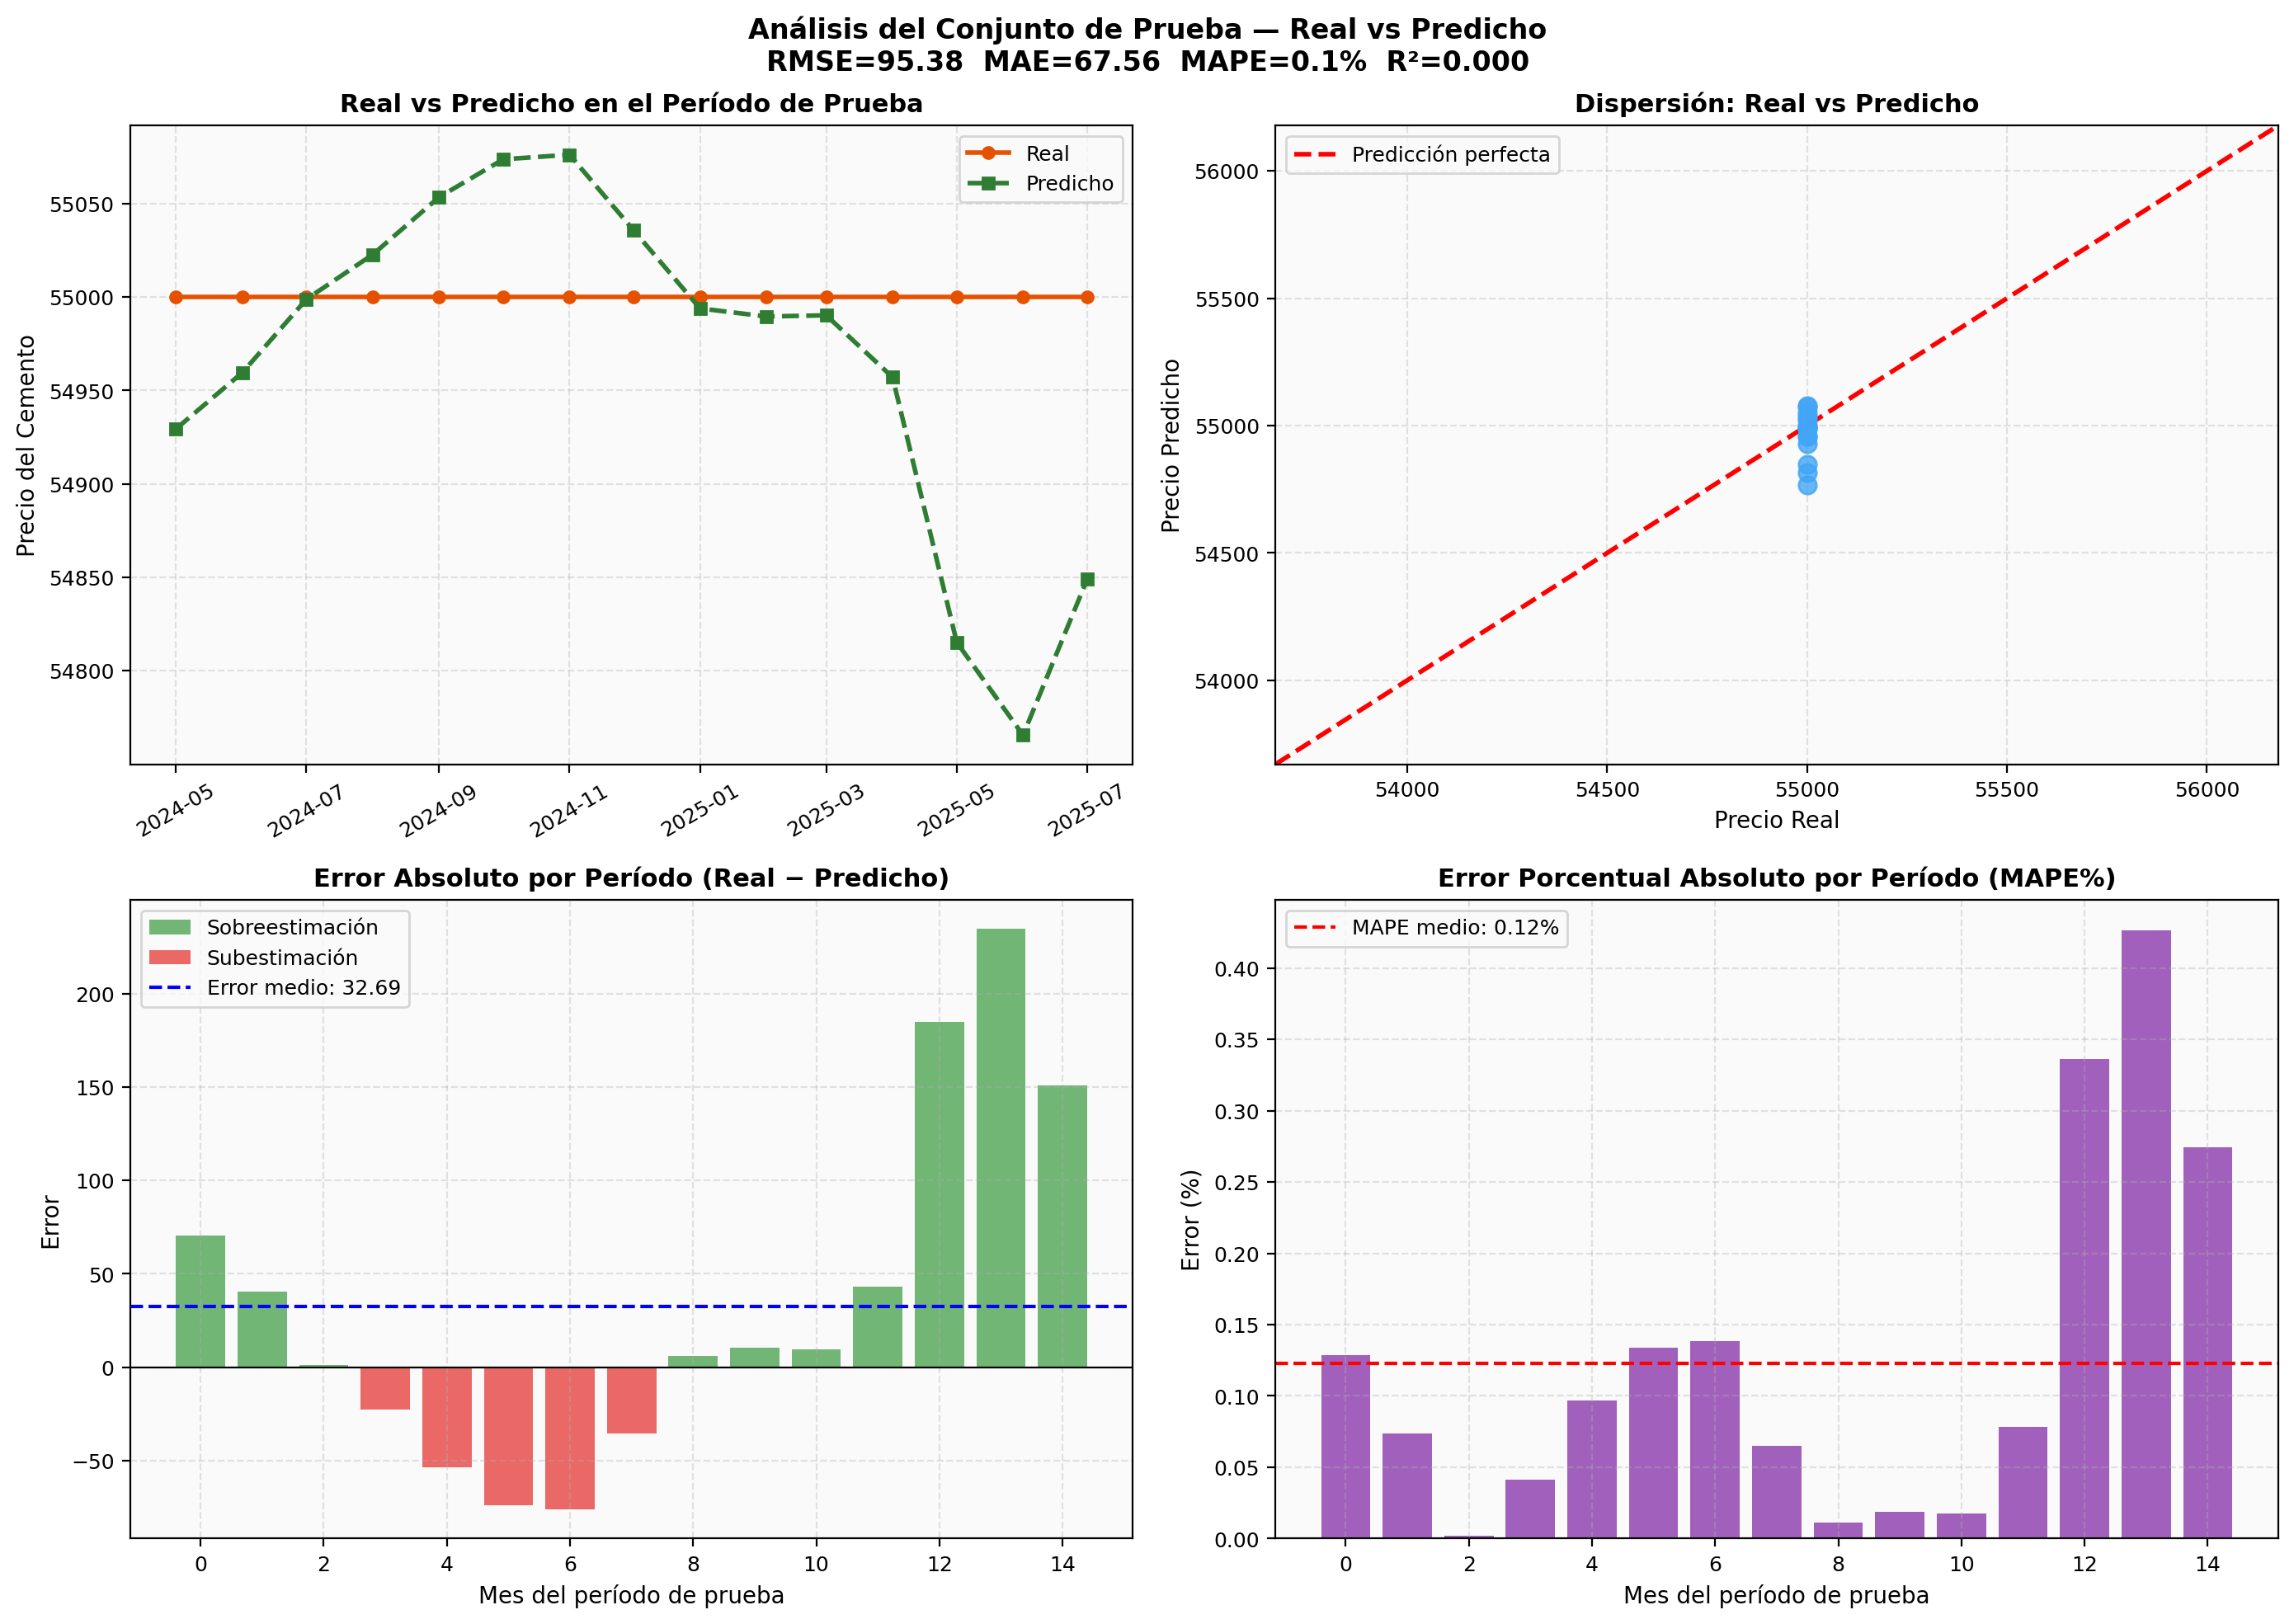
\includegraphics[width=\textwidth]{predicciones/prediccion_sarimax_cemento/graficos/08_comparacion_real_predicho.png}
    \caption{Comparación entre los valores reales y predichos del precio del cemento en el conjunto de prueba (15 meses).}
    \label{fig:sarimax_comparacion}
\end{figure}

\justify
La Figura \ref{fig:sarimax_comparacion} presenta la comparación entre los valores reales y los predichos por el modelo sobre el conjunto de prueba, que comprende los últimos 15 meses de la serie. Las métricas de evaluación obtenidas se resumen en la Tabla \ref{tab:sarimax_metricas_prueba}.

\begin{table}[ht]
    \centering
    \caption{Métricas de evaluación del modelo SARIMAX sobre el conjunto de prueba (15 meses).}
    \label{tab:sarimax_metricas_prueba}
    \begin{tabular}{lc}
        \toprule
        \textbf{Métrica} & \textbf{Valor} \\
        \midrule
        RMSE (Raíz del Error Cuadrático Medio) & 95{,}38~Gs. \\
        MAE  (Error Absoluto Medio)            & 67{,}56~Gs. \\
        MAPE (Error Porcentual Medio Absoluto) & 0{,}12\,\% \\
        SMAPE (Error Porcentual Simétrico)     & 0{,}12\,\% \\
        Error Absoluto Máximo                  & 234{,}47~Gs. \\
        $R^{2}$ (Coeficiente de Determinación) & 0{,}0000 \\
        \bottomrule
    \end{tabular}
\end{table}

\justify
El MAPE de 0{,}12\,\% sobre el conjunto de prueba merece una lectura cuidadosa. Tomado en aislamiento, parece un resultado excelente: las predicciones se alejan poco más de una décima de punto porcentual del valor real. El RMSE de 95{,}38~Gs. y el MAE de 67{,}56~Gs. también son bajos respecto al rango histórico de la serie (Gs.~48.000--76.036). Sin embargo, el $R^{2}=0$ en el mismo período llama la atención: ¿cómo puede el modelo tener un error relativo tan bajo y al mismo tiempo un $R^{2}$ nulo?

\justify
La explicación es que, en el período de prueba, el precio del cemento se mantuvo prácticamente estable — varianza muy baja — de modo que cualquier predicción constante cercana al nivel reciente resultará en errores absolutos pequeños, pero sin diferenciarse del simple promedio histórico en términos de varianza explicada. En otras palabras, el contexto del mercado durante ese período limitó lo que cualquier modelo, no solo el SARIMAX, podía demostrar. El comportamiento es además coherente con el orden $(0,1,0)$ seleccionado: sin términos AR ni MA, el modelo proyecta básicamente el último valor observado, que es la estrategia óptima cuando la serie diferenciada se comporta como ruido blanco. La validación cruzada, que sí abarca períodos con mayor variabilidad, ofrece una imagen más completa del desempeño real.

\subsubsection{Modelo SARIMAX: Validación Cruzada}

\begin{figure}[ht]
    \centering
    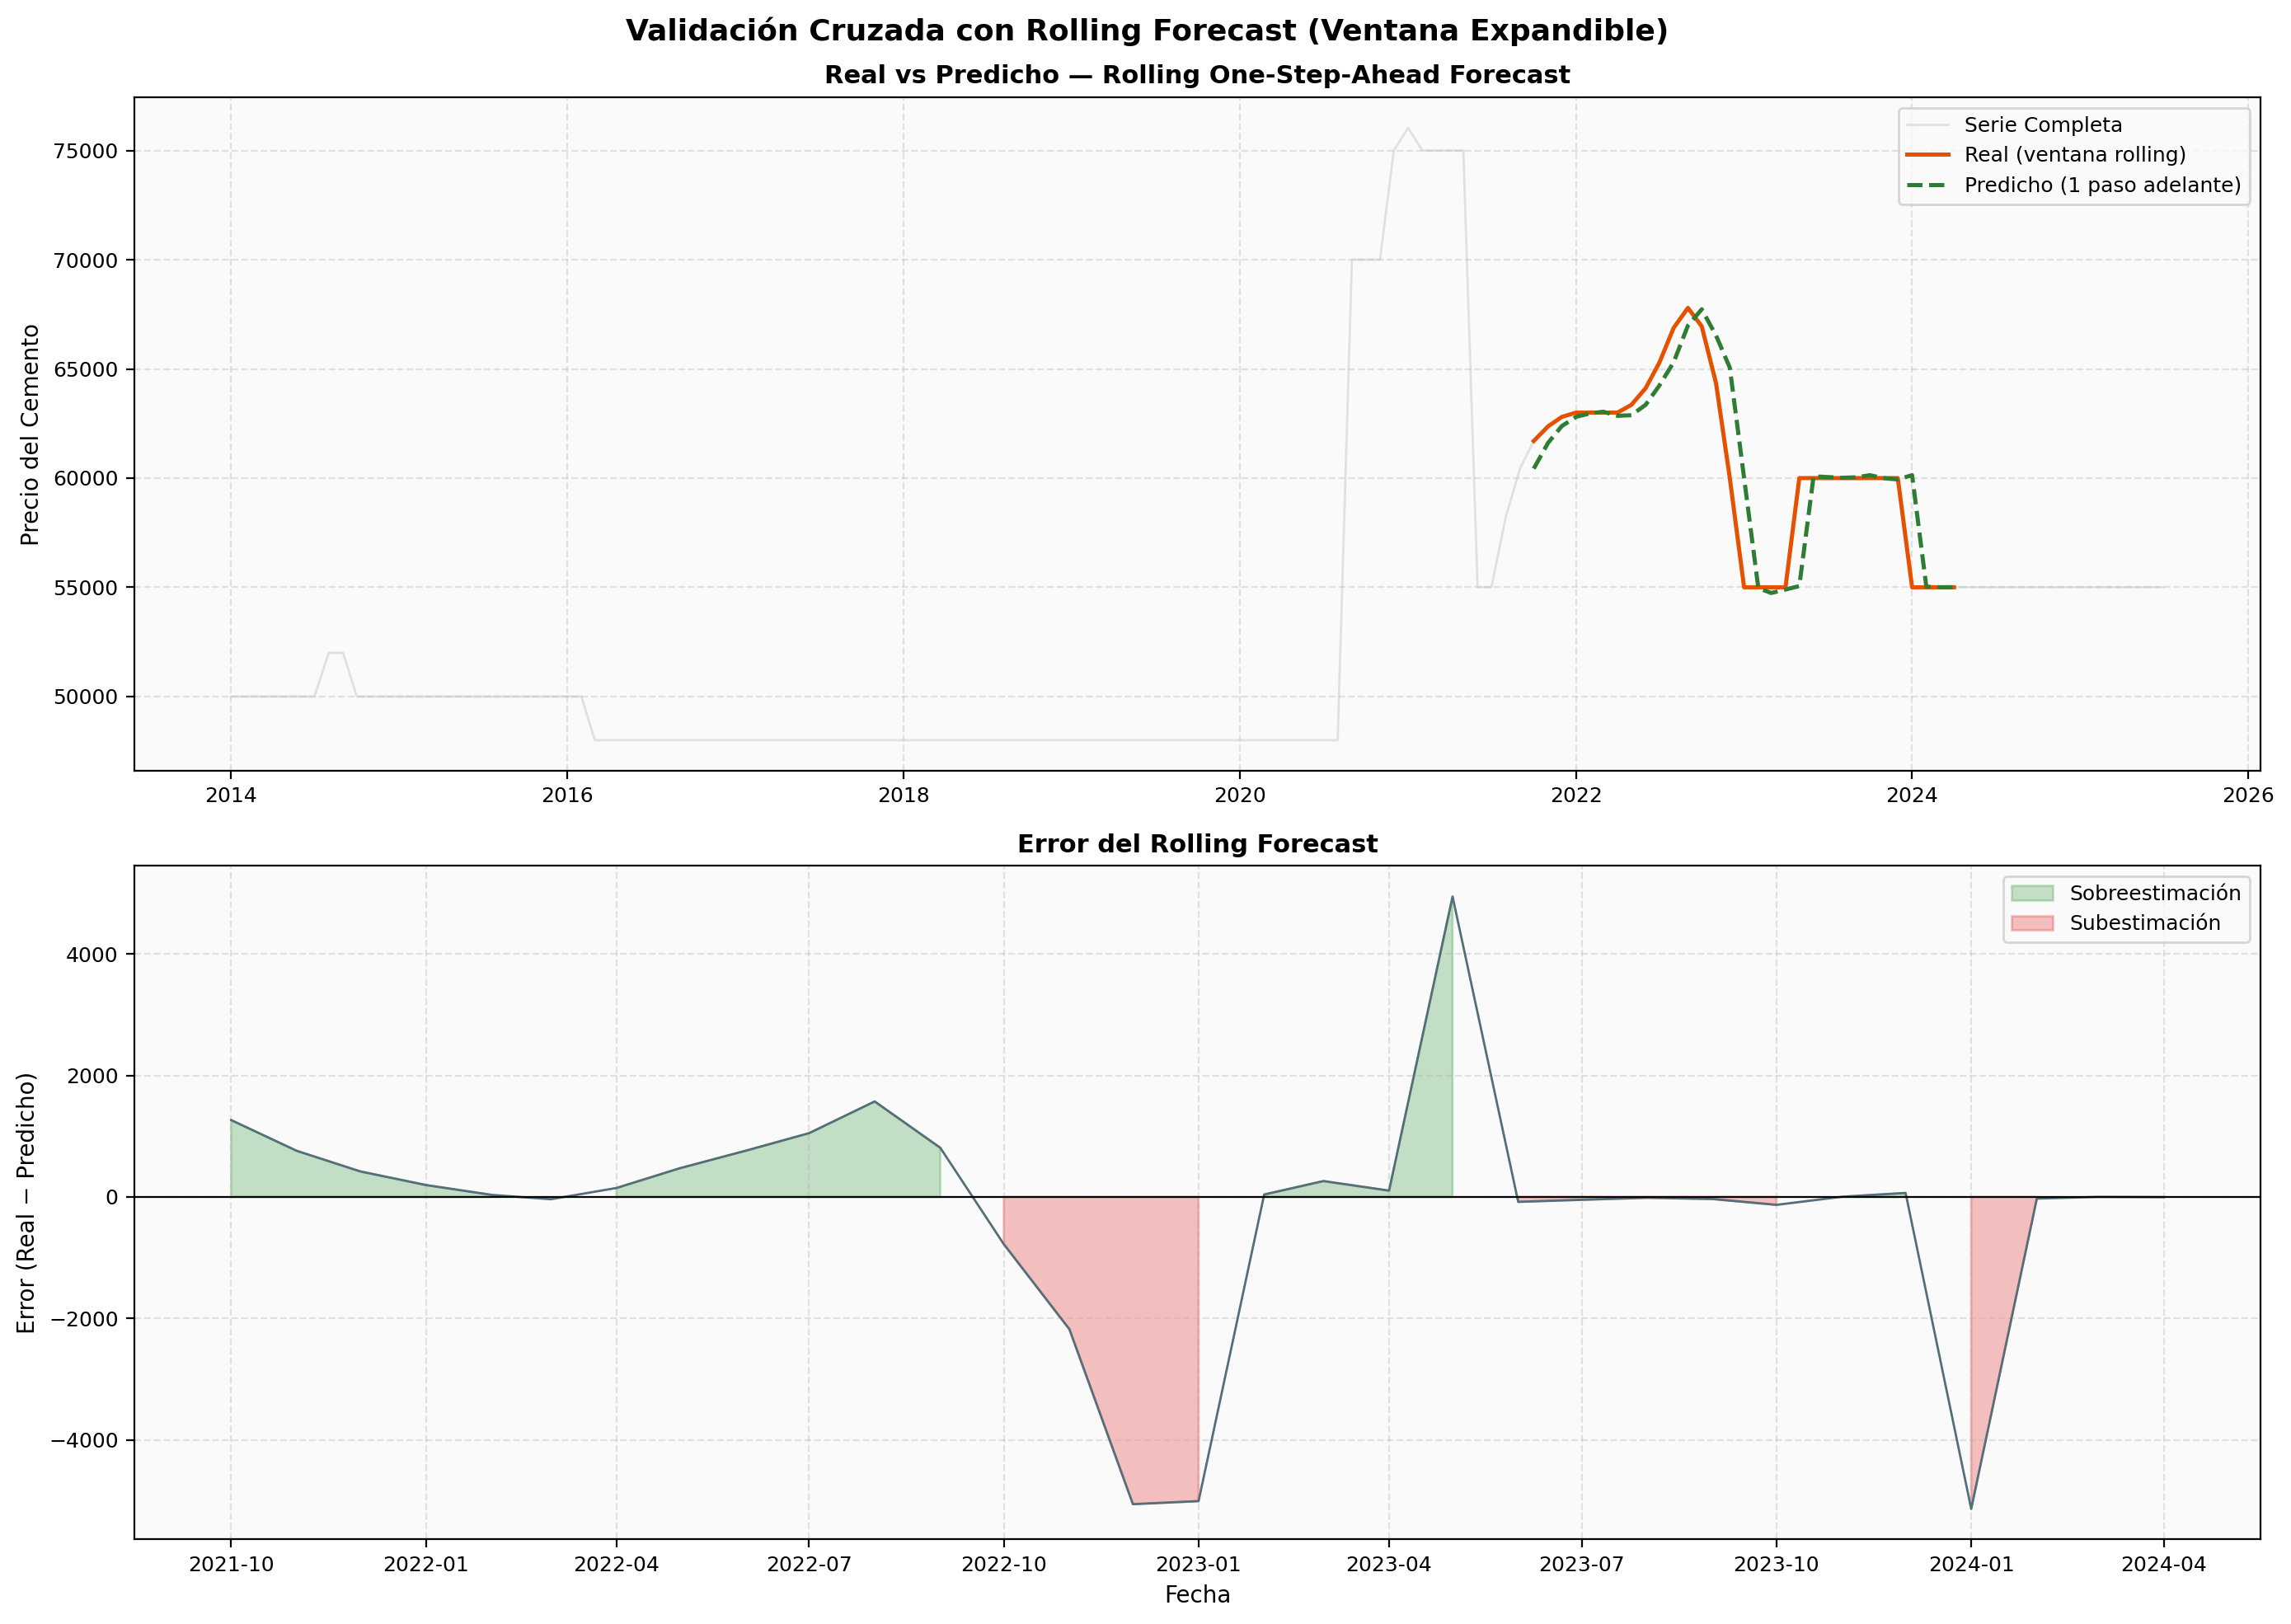
\includegraphics[width=\textwidth]{predicciones/prediccion_sarimax_cemento/graficos/10_rolling_forecast_cv.png}
    \caption{Validación cruzada por ventana deslizante (\textit{rolling forecast}): predicciones puntuales versus valores reales en cada paso de avance.}
    \label{fig:sarimax_rolling}
\end{figure}

\justify
Con el fin de obtener una estimación más robusta de la capacidad predictiva del modelo, se aplicó una validación cruzada por ventana deslizante (\textit{rolling forecast}), en la que el modelo se re-estima en cada paso incorporando las observaciones disponibles hasta ese momento y genera una predicción un paso adelante. La Figura \ref{fig:sarimax_rolling} ilustra el resultado de este procedimiento. Las métricas obtenidas se presentan en la Tabla \ref{tab:sarimax_metricas_cv}.

\begin{table}[ht]
    \centering
    \caption{Métricas de validación cruzada por ventana deslizante del modelo SARIMAX.}
    \label{tab:sarimax_metricas_cv}
    \begin{tabular}{lc}
        \toprule
        \textbf{Métrica} & \textbf{Valor} \\
        \midrule
        RMSE & 1.920{,}78~Gs. \\
        MAE  & 1.013{,}86~Gs. \\
        MAPE & 1{,}70\,\% \\
        $R^{2}$ & 0{,}7586 \\
        \bottomrule
    \end{tabular}
\end{table}

\justify
Aquí el panorama cambia. Con un $R^{2}=0{,}7586$, el modelo explica el 75{,}86\,\% de la varianza del precio a lo largo de todo el período histórico disponible, incluyendo los años de alta volatilidad. El MAPE de 1{,}70\,\% —muy por debajo del umbral del 5\,\% que suele citarse como referencia para series de precios de materiales— confirma que el SARIMAX tiene utilidad práctica real para la gestión de presupuestos de obra, al menos en escenarios de proyección a un paso adelante.

\subsubsection{Modelo SARIMAX: Análisis de Residuos}

\begin{figure}[ht]
    \centering
    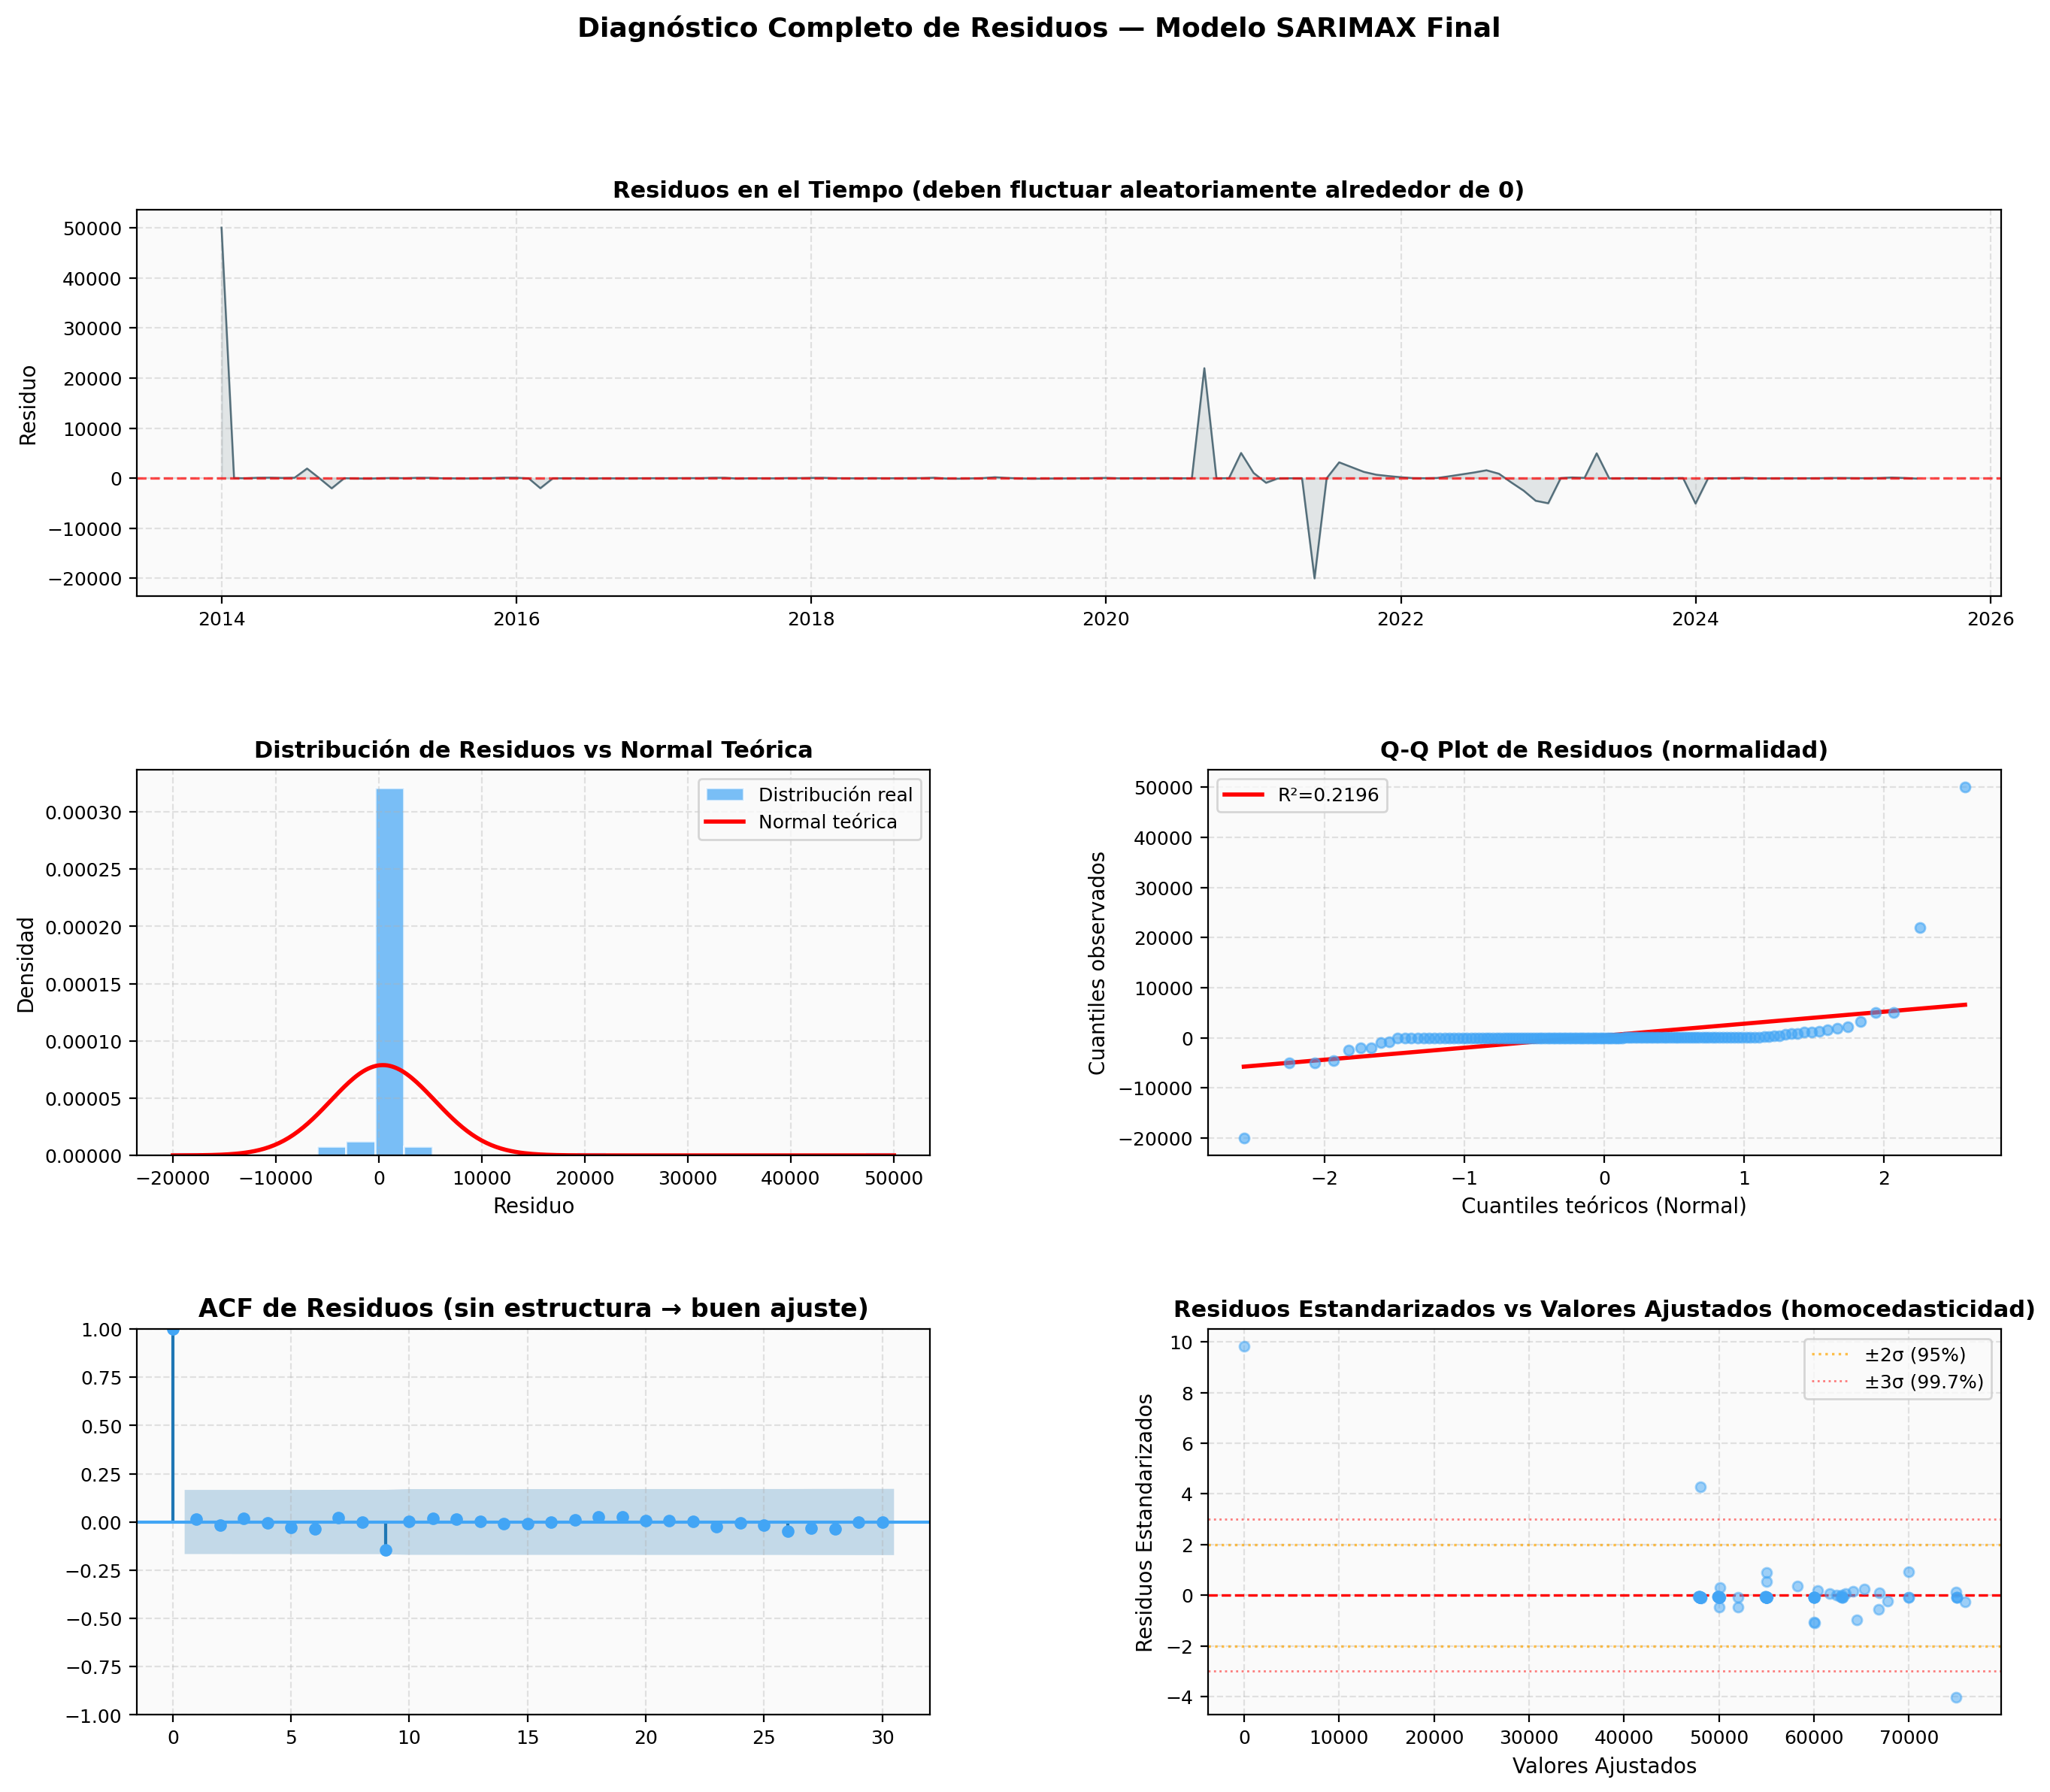
\includegraphics[width=\textwidth]{predicciones/prediccion_sarimax_cemento/graficos/07_diagnostico_residuos.png}
    \caption{Diagnóstico de residuos del modelo SARIMAX: gráfico de residuos, histograma, gráfico Q-Q y función de autocorrelación.}
    \label{fig:sarimax_residuos}
\end{figure}

\justify
La Figura \ref{fig:sarimax_residuos} presenta el diagnóstico completo de los residuos del modelo SARIMAX. El test de Ljung-Box no rechaza la hipótesis nula de ausencia de autocorrelación serial en los residuos para los rezagos 10 ($Q=3{,}77$, $p=0{,}957$) y 20 ($Q=4{,}13$, $p=0{,}9999$), confirmando que los residuos se comportan como ruido blanco y que el modelo ha capturado adecuadamente la estructura dinámica de la serie. Por su parte, el test de Shapiro-Wilk rechaza la normalidad de los residuos ($W=0{,}2404$, $p<0{,}001$), resultado que se explica por la presencia de observaciones extremas durante el período pandémico, las cuales introducen una curtosis elevada (49{,}47) y una asimetría positiva moderada (0{,}83). Esta no normalidad no invalida las estimaciones puntuales del modelo, aunque sí impone cautela en la interpretación de los intervalos de confianza calculados bajo el supuesto gaussiano.

\subsubsection{Modelo SARIMAX: Pronóstico a 24 Meses}

\begin{figure}[ht]
    \centering
    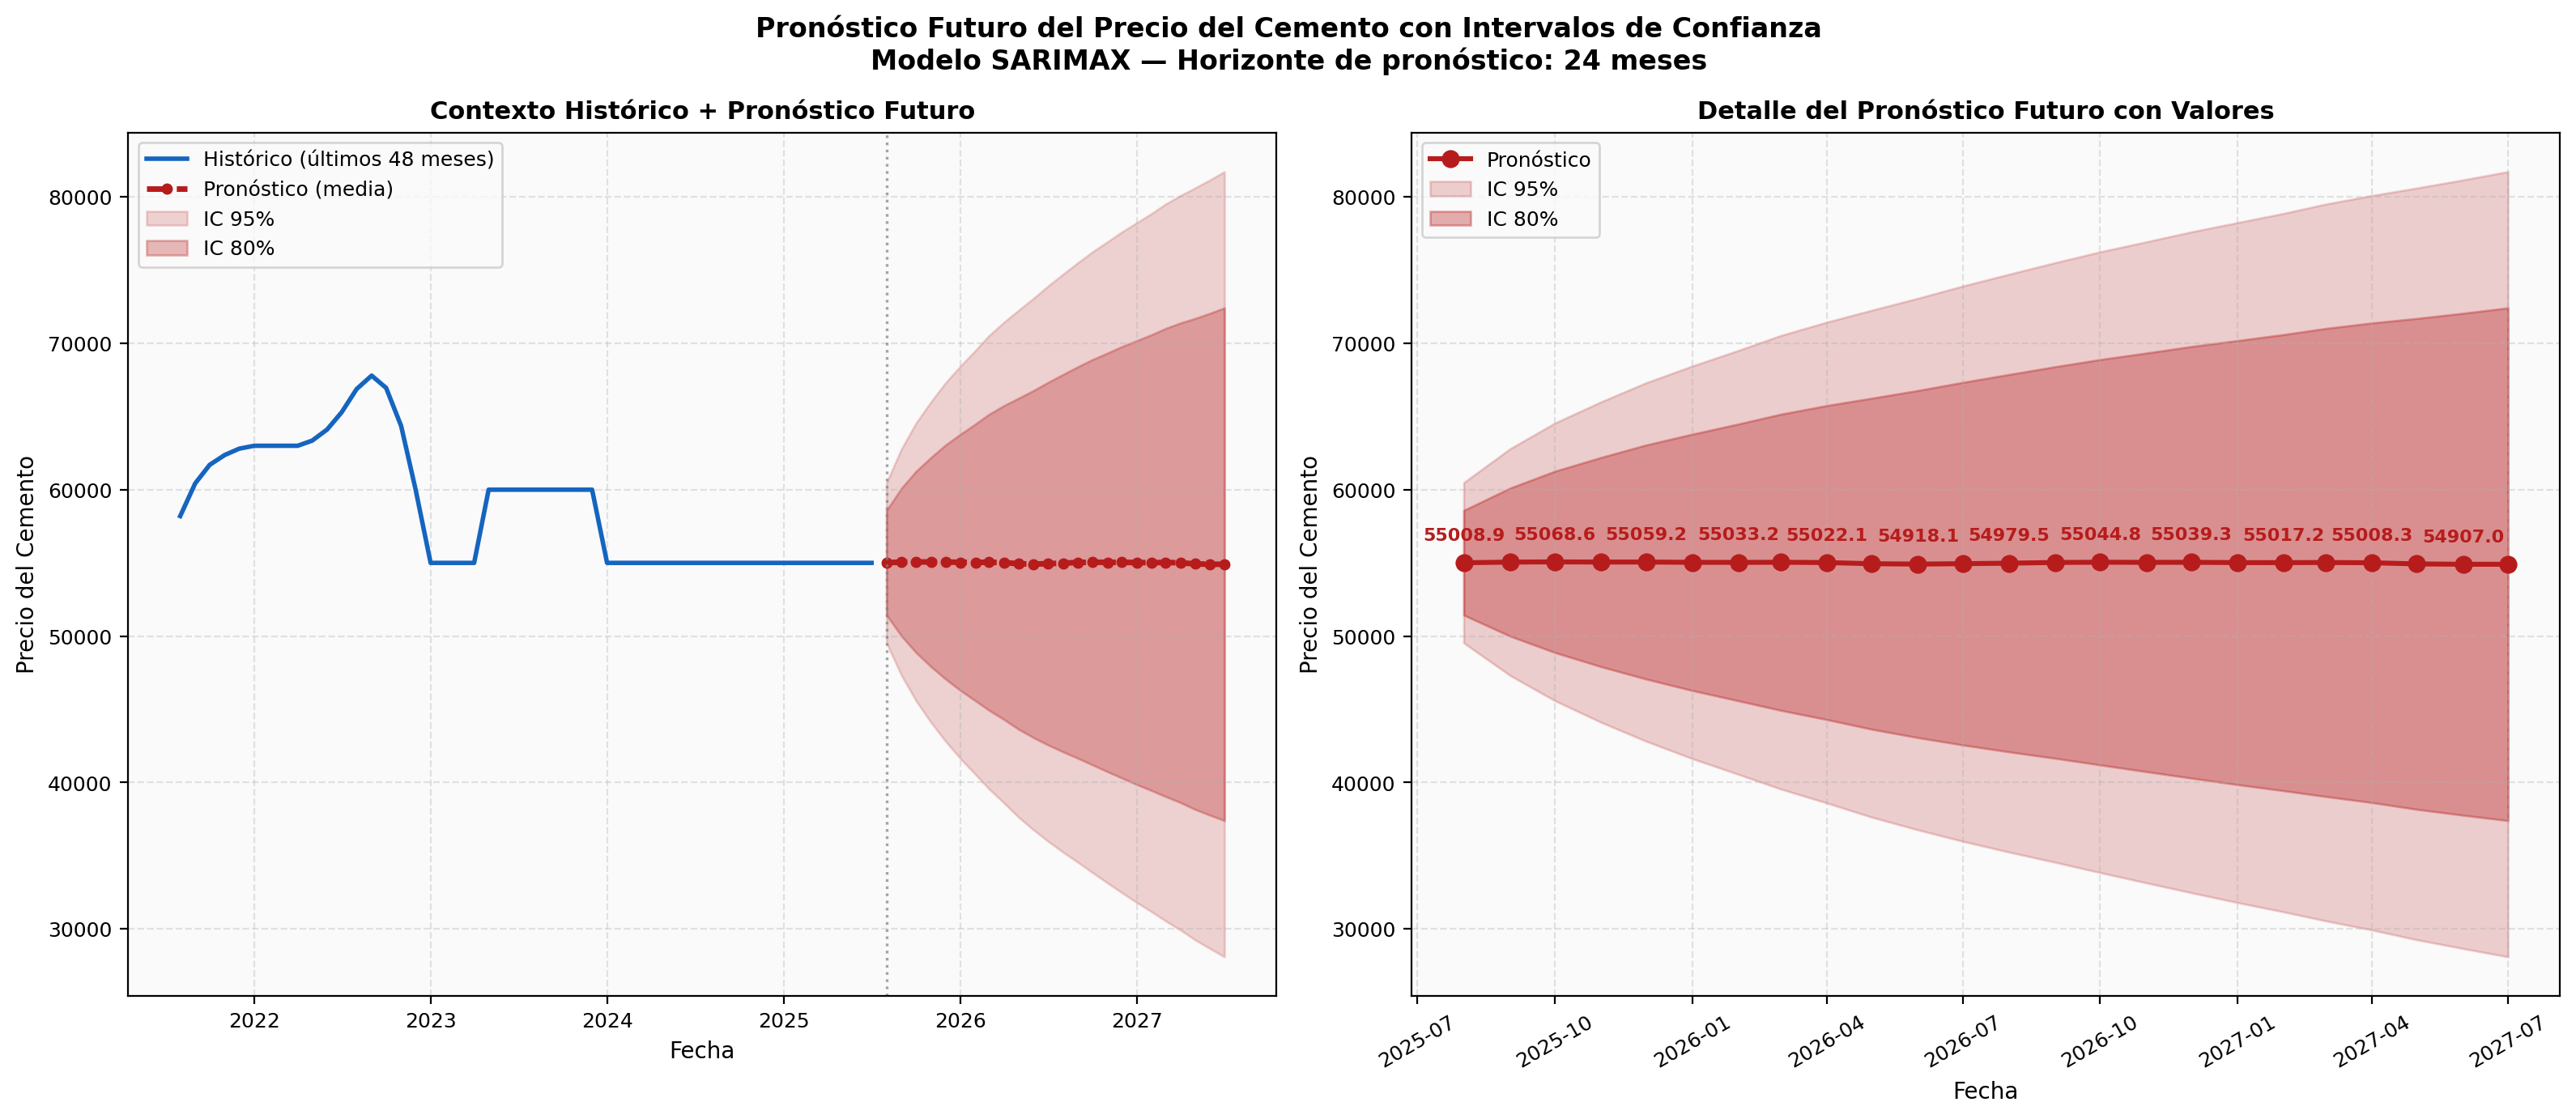
\includegraphics[width=\textwidth]{predicciones/prediccion_sarimax_cemento/graficos/09_pronostico_intervalo_confianza.png}
    \caption{Pronóstico del precio del cemento a 24 meses (agosto 2025 -- julio 2027) con intervalos de confianza al 95\%.}
    \label{fig:sarimax_pronostico_ic}
\end{figure}

\begin{figure}[ht]
    \centering
    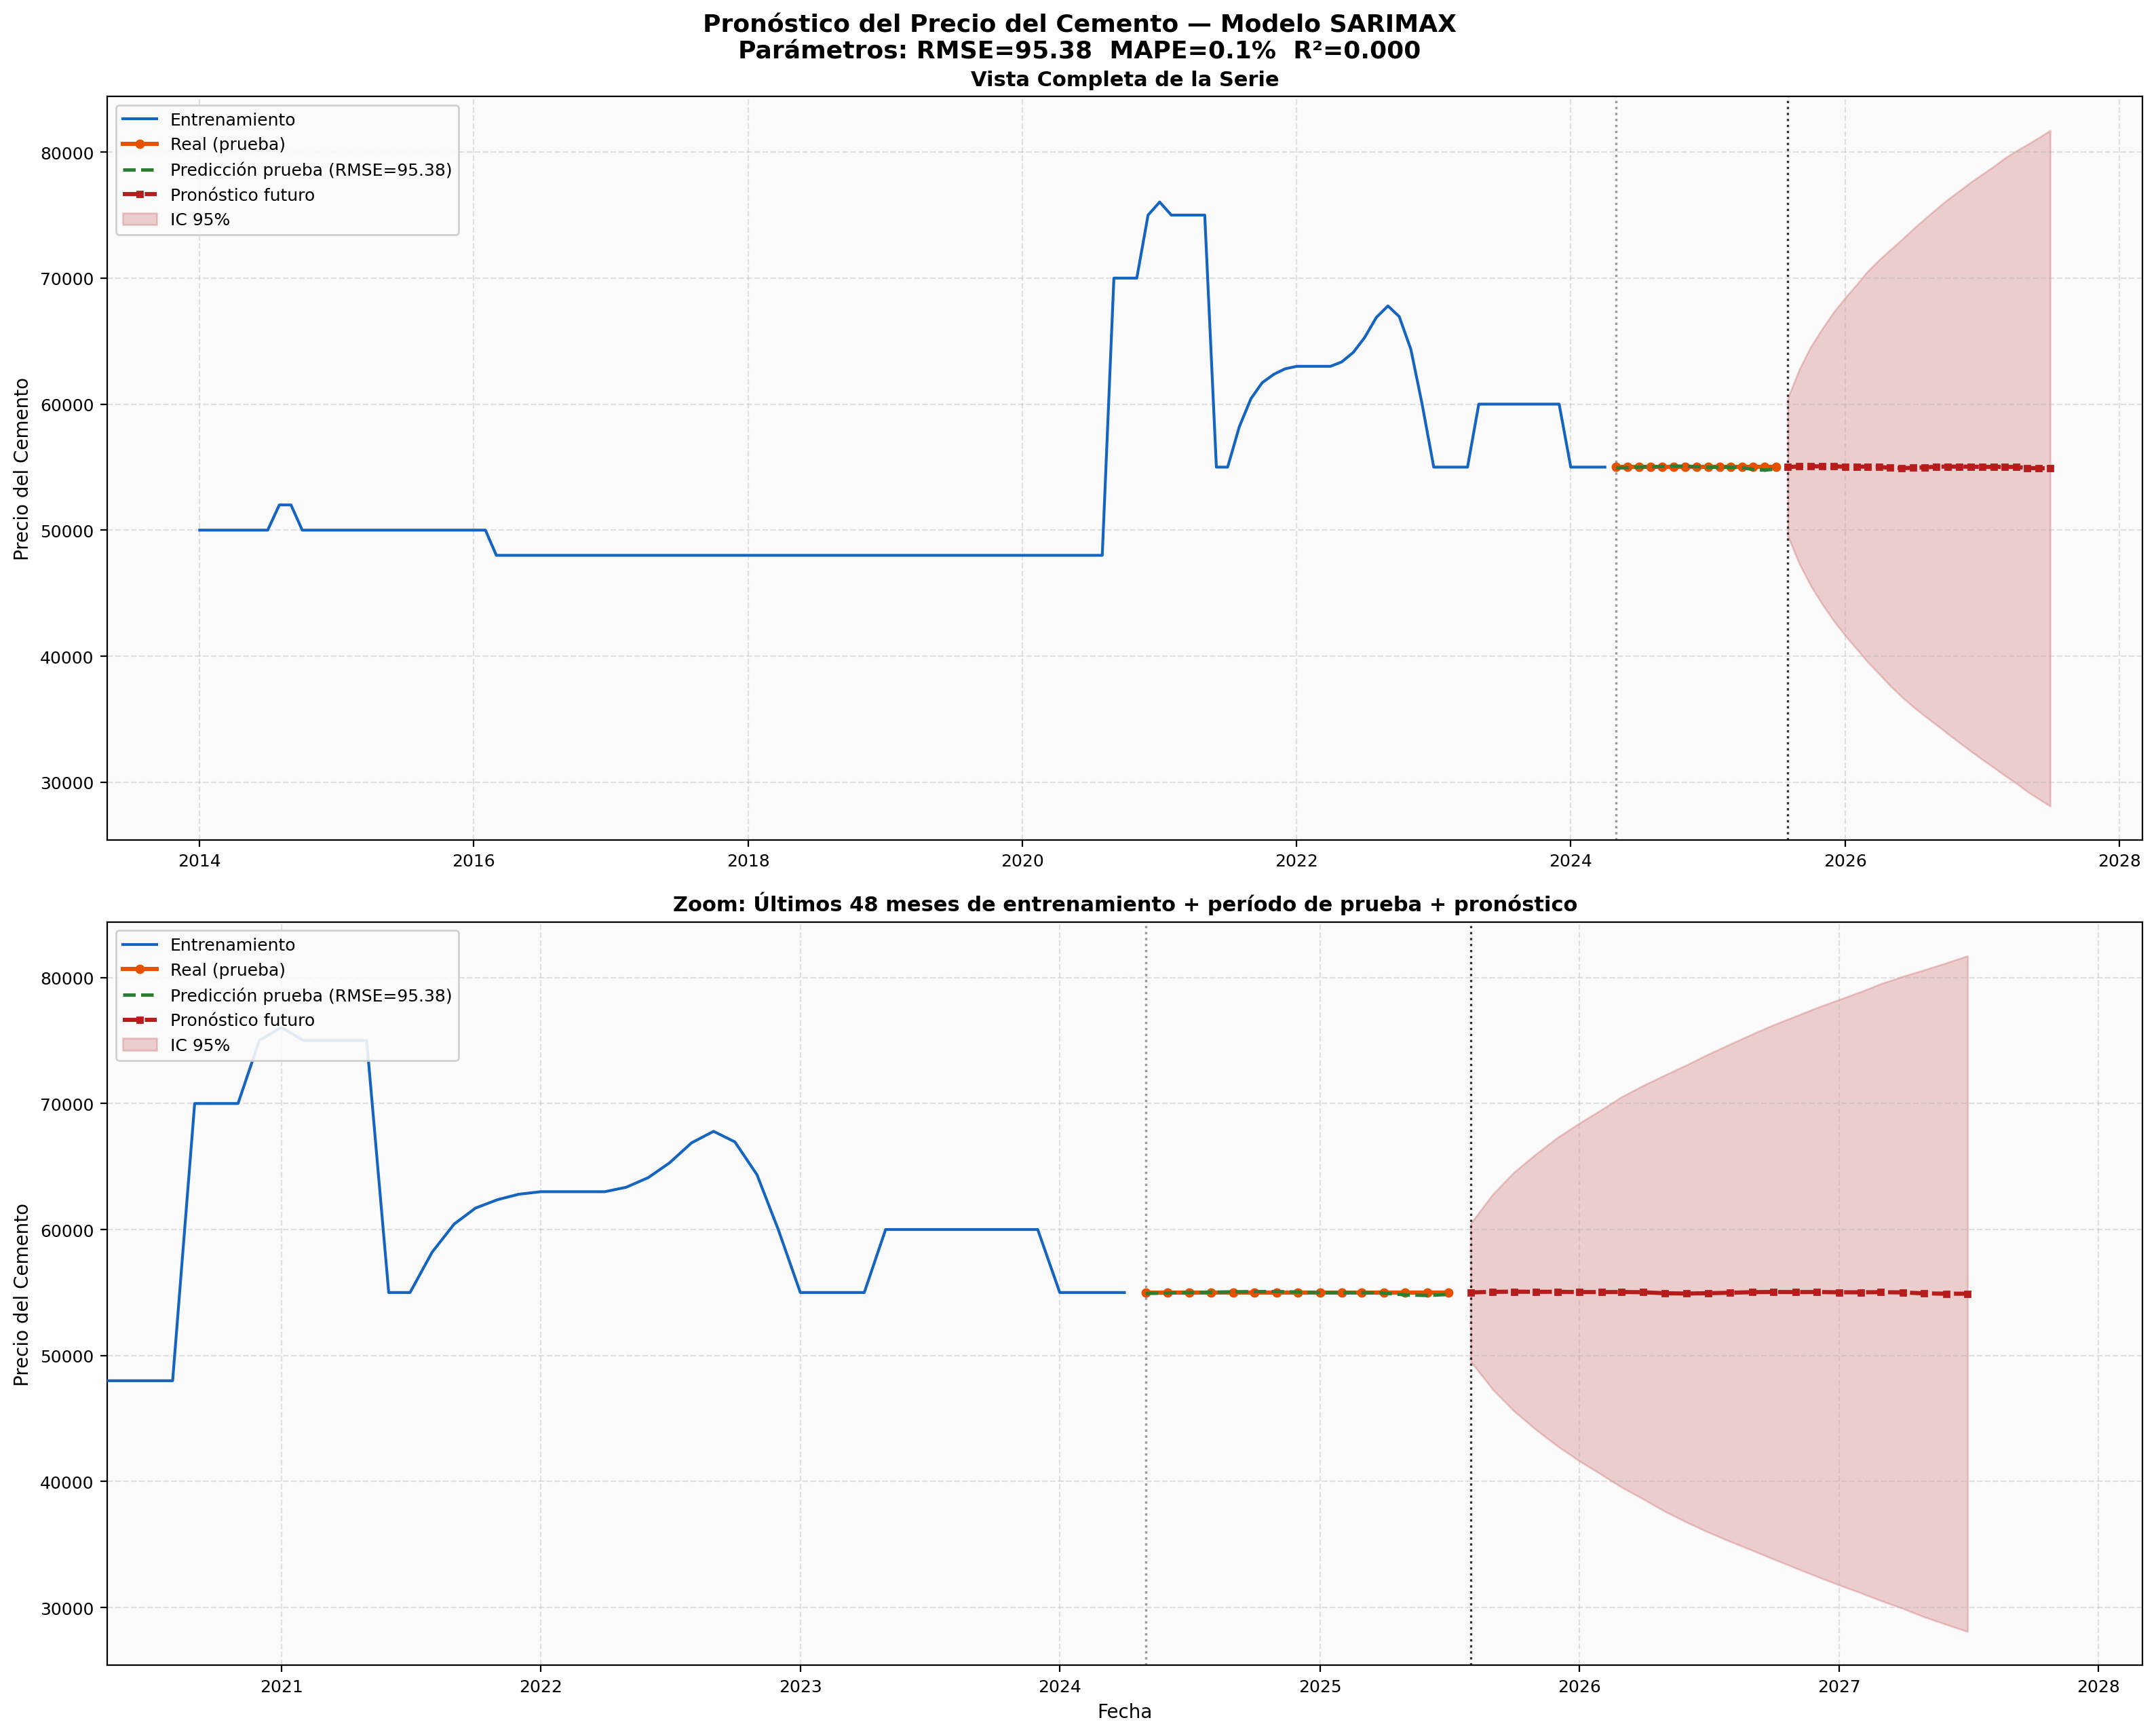
\includegraphics[width=\textwidth]{predicciones/prediccion_sarimax_cemento/graficos/06_pronostico_completo.png}
    \caption{Pronóstico completo del precio del cemento: serie histórica observada y proyección SARIMAX a 24 meses.}
    \label{fig:sarimax_pronostico_completo}
\end{figure}

\justify
Una vez validado el modelo, se generó el pronóstico del precio mensual del cemento para el horizonte de 24 meses comprendido entre agosto de 2025 y julio de 2027, utilizando como variable exógena los niveles del río Paraguay proyectados por el modelo LSTM. Las Figuras \ref{fig:sarimax_pronostico_ic} y \ref{fig:sarimax_pronostico_completo} presentan el pronóstico puntual y el intervalo de confianza al 95\,\%, así como la vista conjunta con la serie histórica completa.

\justify
El pronóstico puntual converge rápidamente hacia un valor estable de aproximadamente Gs.~55.010, consistente con la naturaleza del modelo SARIMAX$(0,1,0)$, cuyas predicciones corresponden a la última observación más la contribución de las variables exógenas proyectadas. El intervalo de confianza al 95\,\% se amplía progresivamente con el horizonte de predicción: para agosto de 2025 el rango es de Gs.~[49.535 -- 60.483], mientras que para julio de 2027 se extiende a Gs.~[28.089 -- 81.724]. Este ensanchamiento, inherente a los modelos integrados en horizontes largos, refleja la incertidumbre acumulada de la proyección y proporciona los límites inferior y superior necesarios para la planificación conservadora y optimista de presupuestos de obra.

\justify
La Tabla \ref{tab:sarimax_pronostico} sintetiza los valores pronosticados para los primeros doce meses del horizonte de predicción.

\begin{table}[ht]
    \centering
    \caption{Pronóstico mensual del precio del cemento (Gs.) para el período agosto 2025 -- julio 2026, con intervalo de confianza al 95\,\%.}
    \label{tab:sarimax_pronostico}
    \begin{tabular}{lccc}
        \toprule
        \textbf{Mes} & \textbf{Pronóstico (Gs.)} & \textbf{IC Inferior} & \textbf{IC Superior} \\
        \midrule
        Agosto 2025      & 55.009 & 49.535 & 60.483 \\
        Septiembre 2025  & 55.053 & 47.311 & 62.794 \\
        Octubre 2025     & 55.069 & 45.587 & 64.550 \\
        Noviembre 2025   & 55.055 & 44.107 & 66.003 \\
        Diciembre 2025   & 55.059 & 42.819 & 67.299 \\
        Enero 2026       & 55.037 & 41.628 & 68.445 \\
        Febrero 2026     & 55.033 & 40.550 & 69.516 \\
        Marzo 2026       & 55.041 & 39.558 & 70.524 \\
        Abril 2026       & 55.022 & 38.600 & 71.444 \\
        Mayo 2026        & 54.942 & 37.632 & 72.253 \\
        Junio 2026       & 54.918 & 36.763 & 73.073 \\
        Julio 2026       & 54.946 & 35.983 & 73.908 \\
        \bottomrule
    \end{tabular}
\end{table}

\subsubsection{Modelo SARIMAX: Escenarios con y sin Efecto Pandémico}

\justify
Con el fin de evaluar la sensibilidad del pronóstico SARIMAX ante el \textit{shock} pandémico, se generaron dos proyecciones paralelas: una con la variable \texttt{Cuarentena} fijada en cero (escenario sin pandemia) y otra con esta variable activa durante todo el horizonte de pronóstico (escenario con efecto pandémico). Las Figuras \ref{fig:sarimax_cemento_sin_covid} y \ref{fig:sarimax_cemento_con_covid} presentan los pronósticos resultantes para cada escenario.

\begin{figure}[ht]
    \centering
    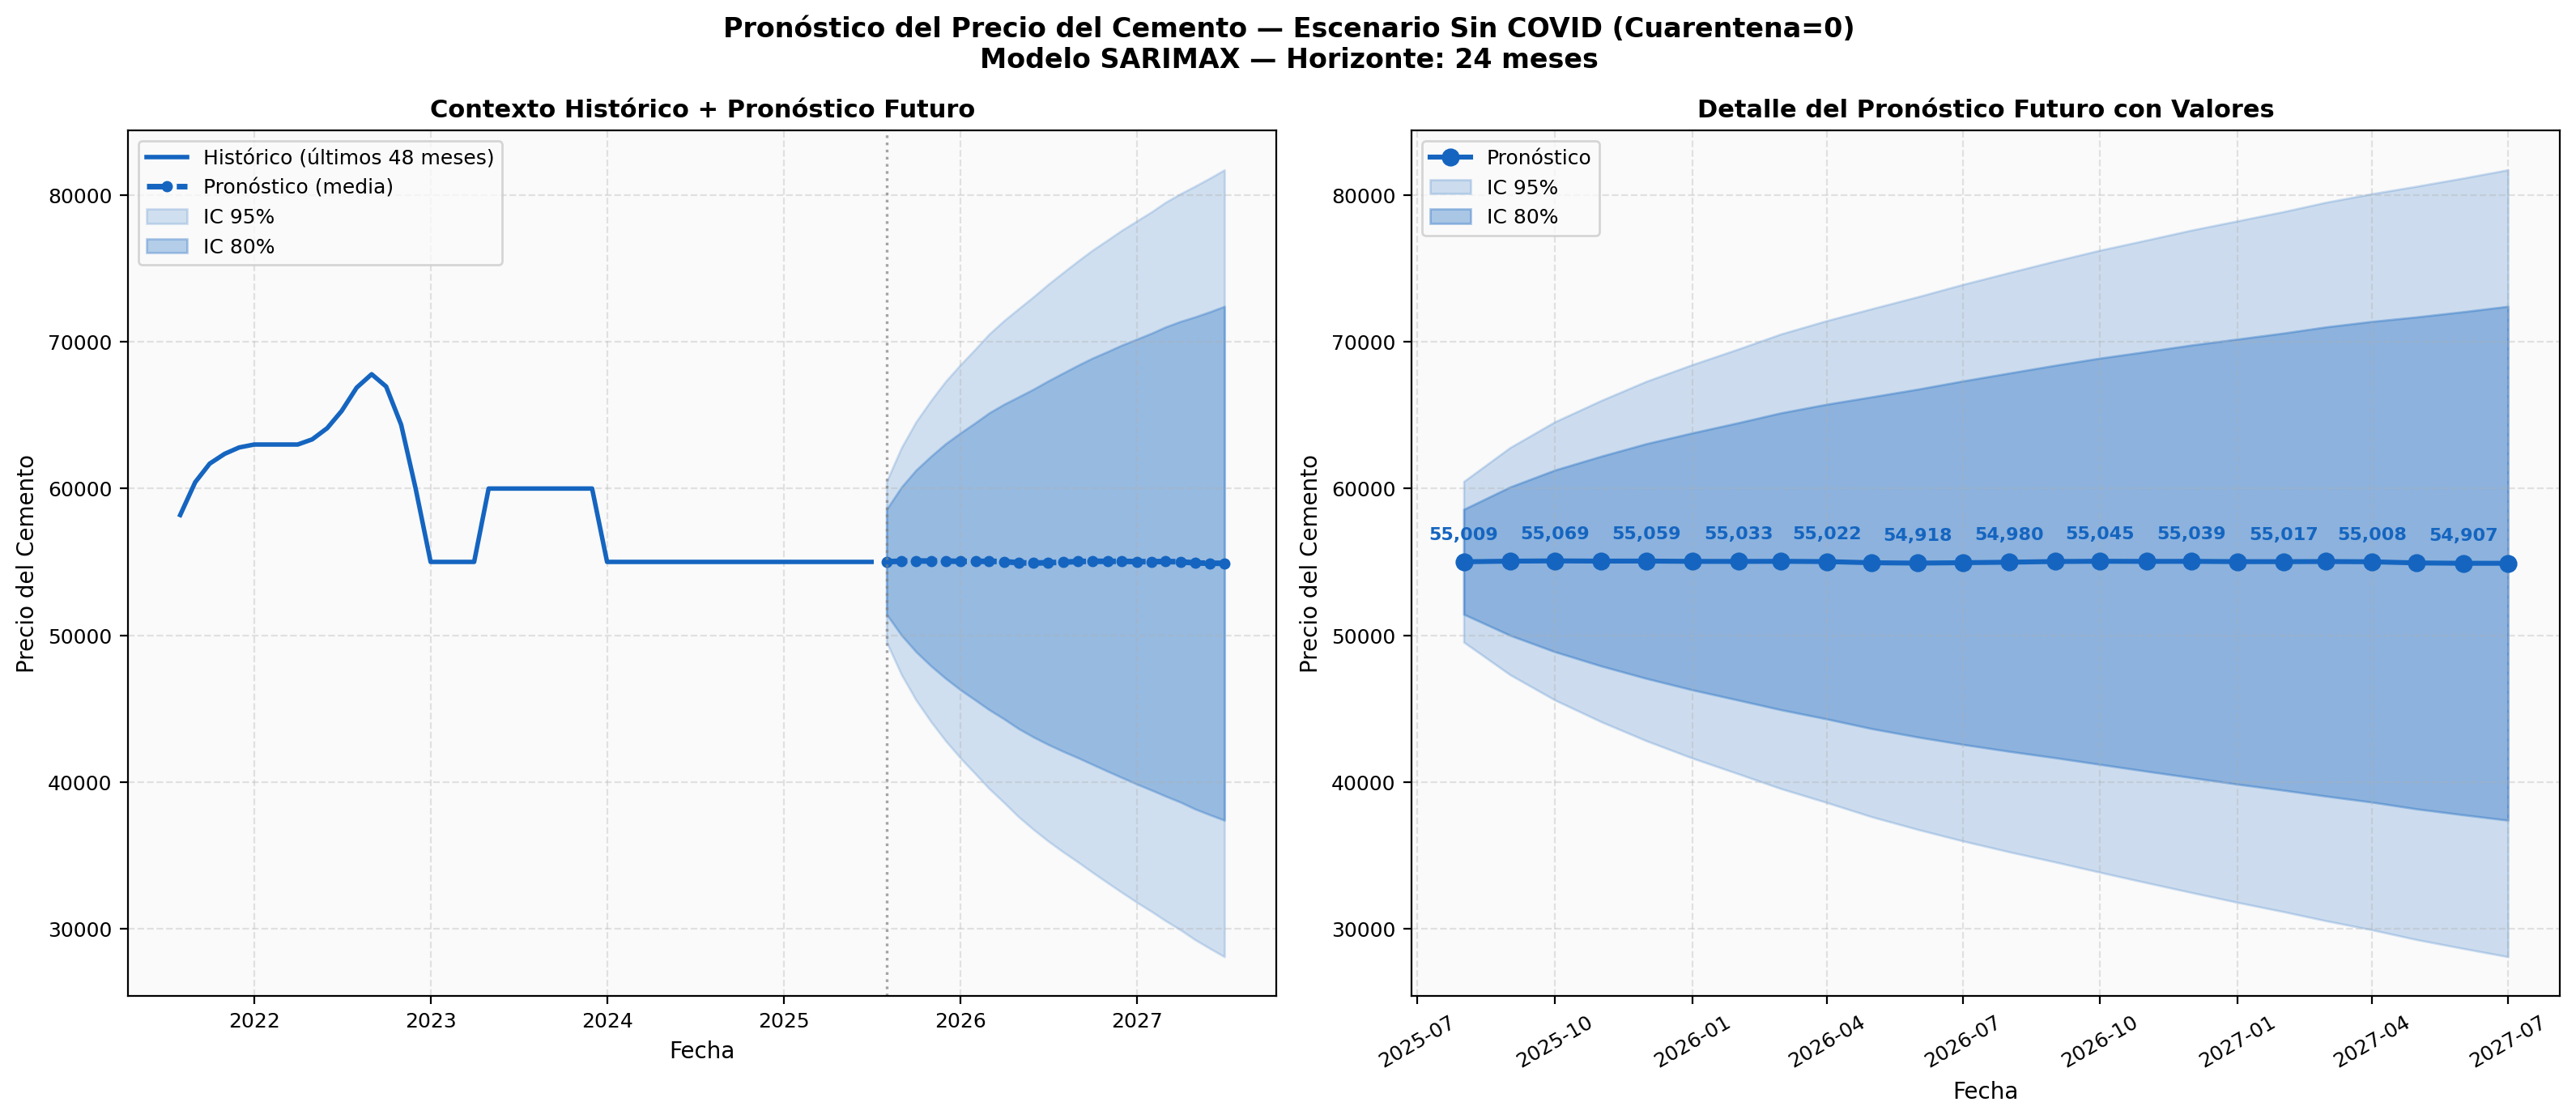
\includegraphics[width=\textwidth]{predicciones/prediccion_sarimax_cemento/graficos/12a_pronostico_sin_covid.png}
    \caption{Pronóstico SARIMAX del precio del cemento a 24 meses -- escenario sin efecto pandémico.}
    \label{fig:sarimax_cemento_sin_covid}
\end{figure}

\begin{figure}[ht]
    \centering
    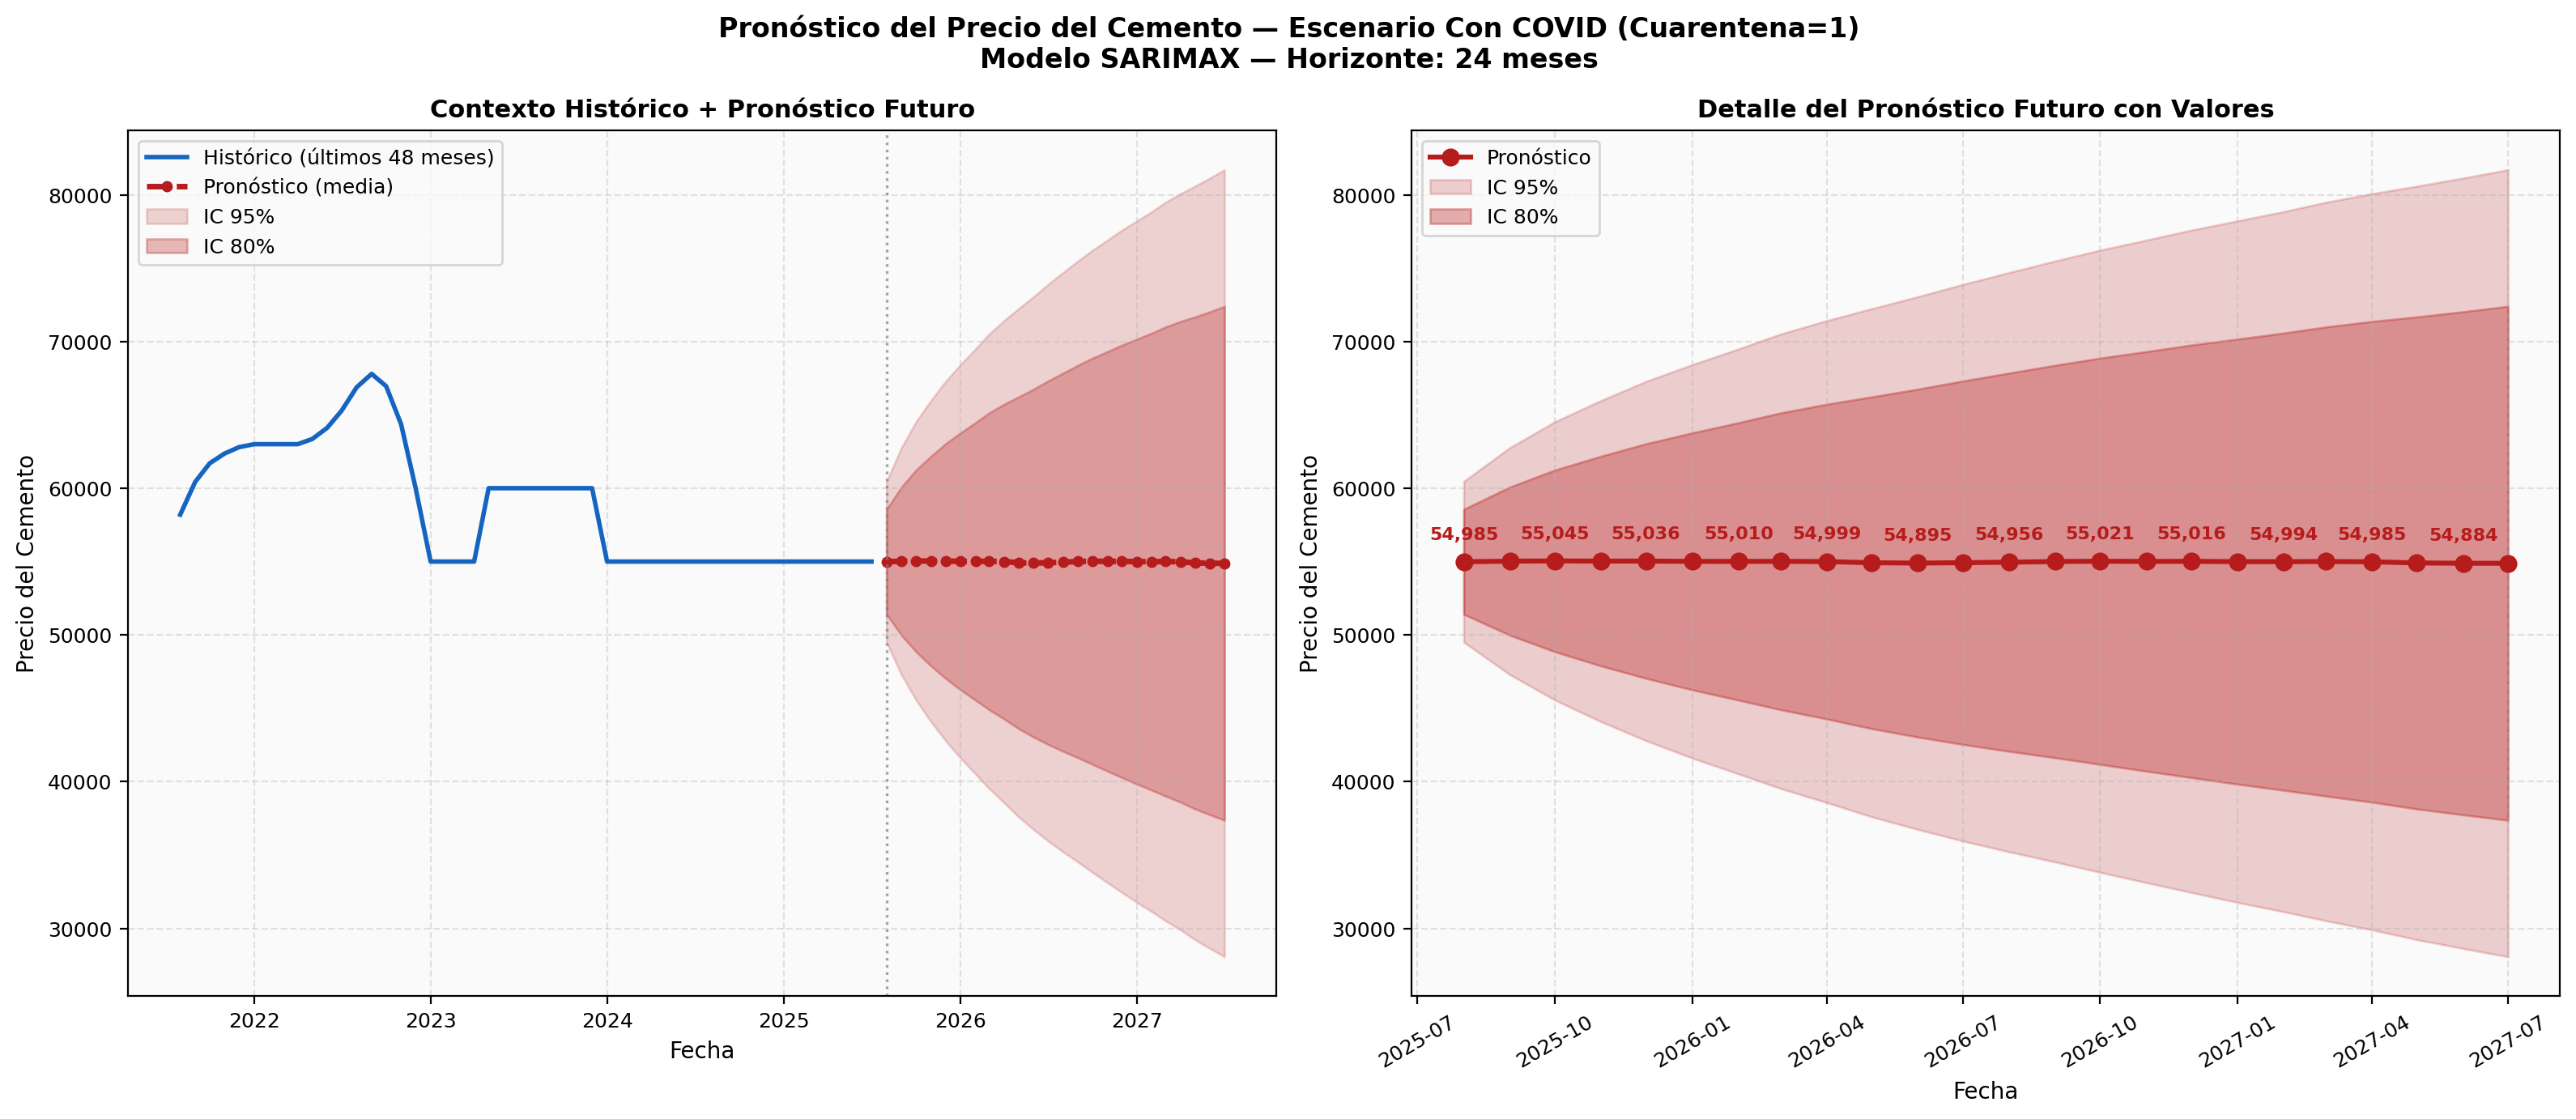
\includegraphics[width=\textwidth]{predicciones/prediccion_sarimax_cemento/graficos/12b_pronostico_con_covid.png}
    \caption{Pronóstico SARIMAX del precio del cemento a 24 meses -- escenario con efecto pandémico.}
    \label{fig:sarimax_cemento_con_covid}
\end{figure}

\justify
El resultado es revelador: la diferencia entre ambos escenarios es de apenas Gs.~$-23{,}48$ por mes, un valor prácticamente despreciable frente al nivel de precios de la serie (Gs.~55.000). Esta diferencia mínima es consistente con el hecho de que el coeficiente estimado para la variable \texttt{Cuarentena} en el modelo SARIMAX resultó estadísticamente no significativo ($p=1{,}000$), como se documentó en la Tabla \ref{tab:sarimax_params}. En otras palabras, el modelo lineal integrado no logra capturar el efecto estructural de la pandemia sobre los precios, dado que la mayor parte de ese impacto queda absorbida por la diferenciación de la serie ($d=1$). Esta limitación del SARIMAX para representar \textit{shocks} exógenos persistentes constituye una de las motivaciones principales para explorar los modelos de aprendizaje profundo, los cuales sí pueden capturar interacciones no lineales entre la variable pandémica y la dinámica de precios.

% ============================================================
\subsection{Predicción del Precio del Ladrillo}
\vspace{0.3cm}
\justify
Además del cemento, se modeló el precio del ladrillo ---segundo insumo clave en la construcción--- utilizando el mismo enfoque SARIMAX. La serie histórica, las variables explicativas y los procedimientos de evaluación siguen la estructura descrita para el cemento, lo que permite una comparación directa entre ambos materiales.

\subsubsection{Serie Histórica y Análisis Exploratorio}

\justify
La serie histórica comprende registros mensuales del precio del ladrillo en Guaraníes (Gs.) desde enero de 2014 hasta julio de 2025, totalizando 139 observaciones. La variable endógena es el precio del ladrillo (\texttt{Precio\_Ladrillo}), mientras que las variables exógenas son el nivel promedio mensual del río Paraguay (\texttt{Nivel\_Rio}), obtenido de las predicciones del modelo LSTM, y la variable binaria de cuarentena (\texttt{Cuarentena}). Los estadísticos descriptivos de la serie son: precio mínimo de Gs.~428, precio máximo de Gs.~700, precio promedio de Gs.~592 y desviación estándar de Gs.~76{,}47.

\begin{figure}[ht]
    \centering
    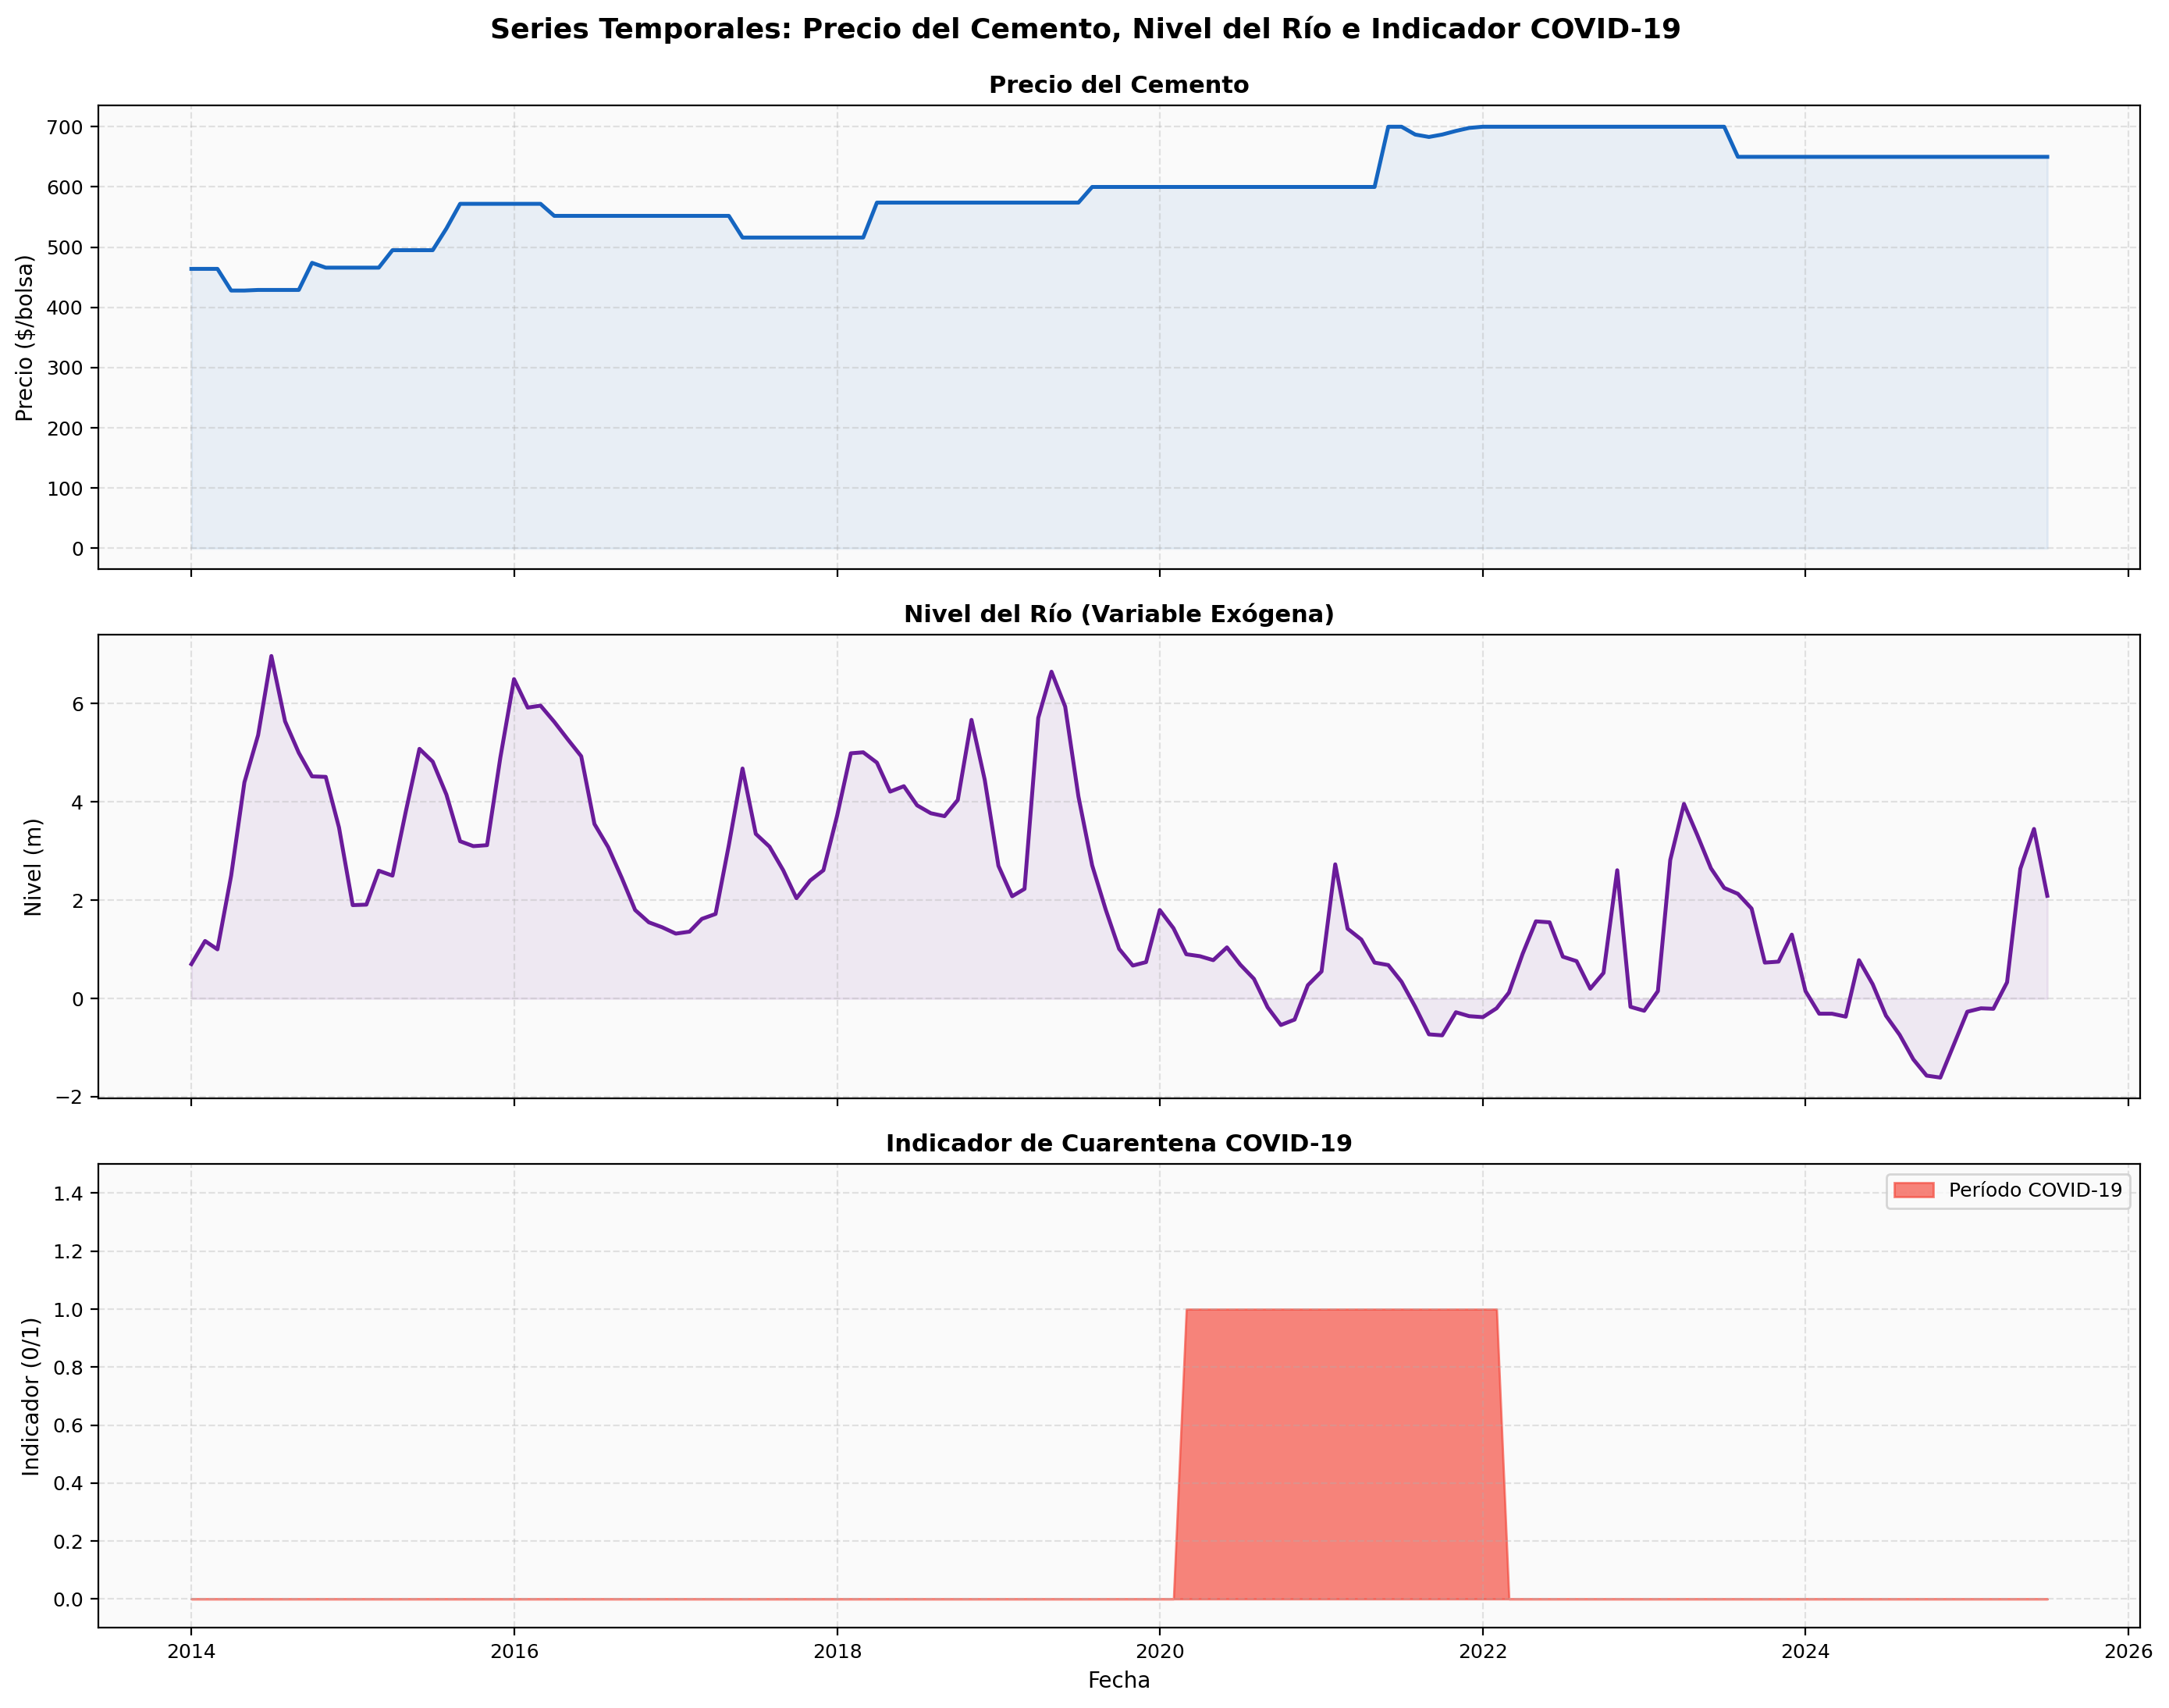
\includegraphics[width=\textwidth]{predicciones/prediccion_sarimax_ladrillo/graficos/01_series_temporales.png}
    \caption{Series temporales del precio mensual del ladrillo (Gs.) y del nivel del río Paraguay (m), período 2014--2025.}
    \label{fig:sarimax_ladrillo_series}
\end{figure}

\justify
La Figura \ref{fig:sarimax_ladrillo_series} muestra la evolución conjunta del precio del ladrillo y del nivel del río Paraguay. Se observa una tendencia ascendente en el precio del ladrillo a lo largo del período analizado, con incrementos escalonados que reflejan los ajustes de precio característicos de este mercado. El precio pasó de aproximadamente Gs.~428 en los primeros años a Gs.~700 hacia el final del período.

\begin{figure}[ht]
    \centering
    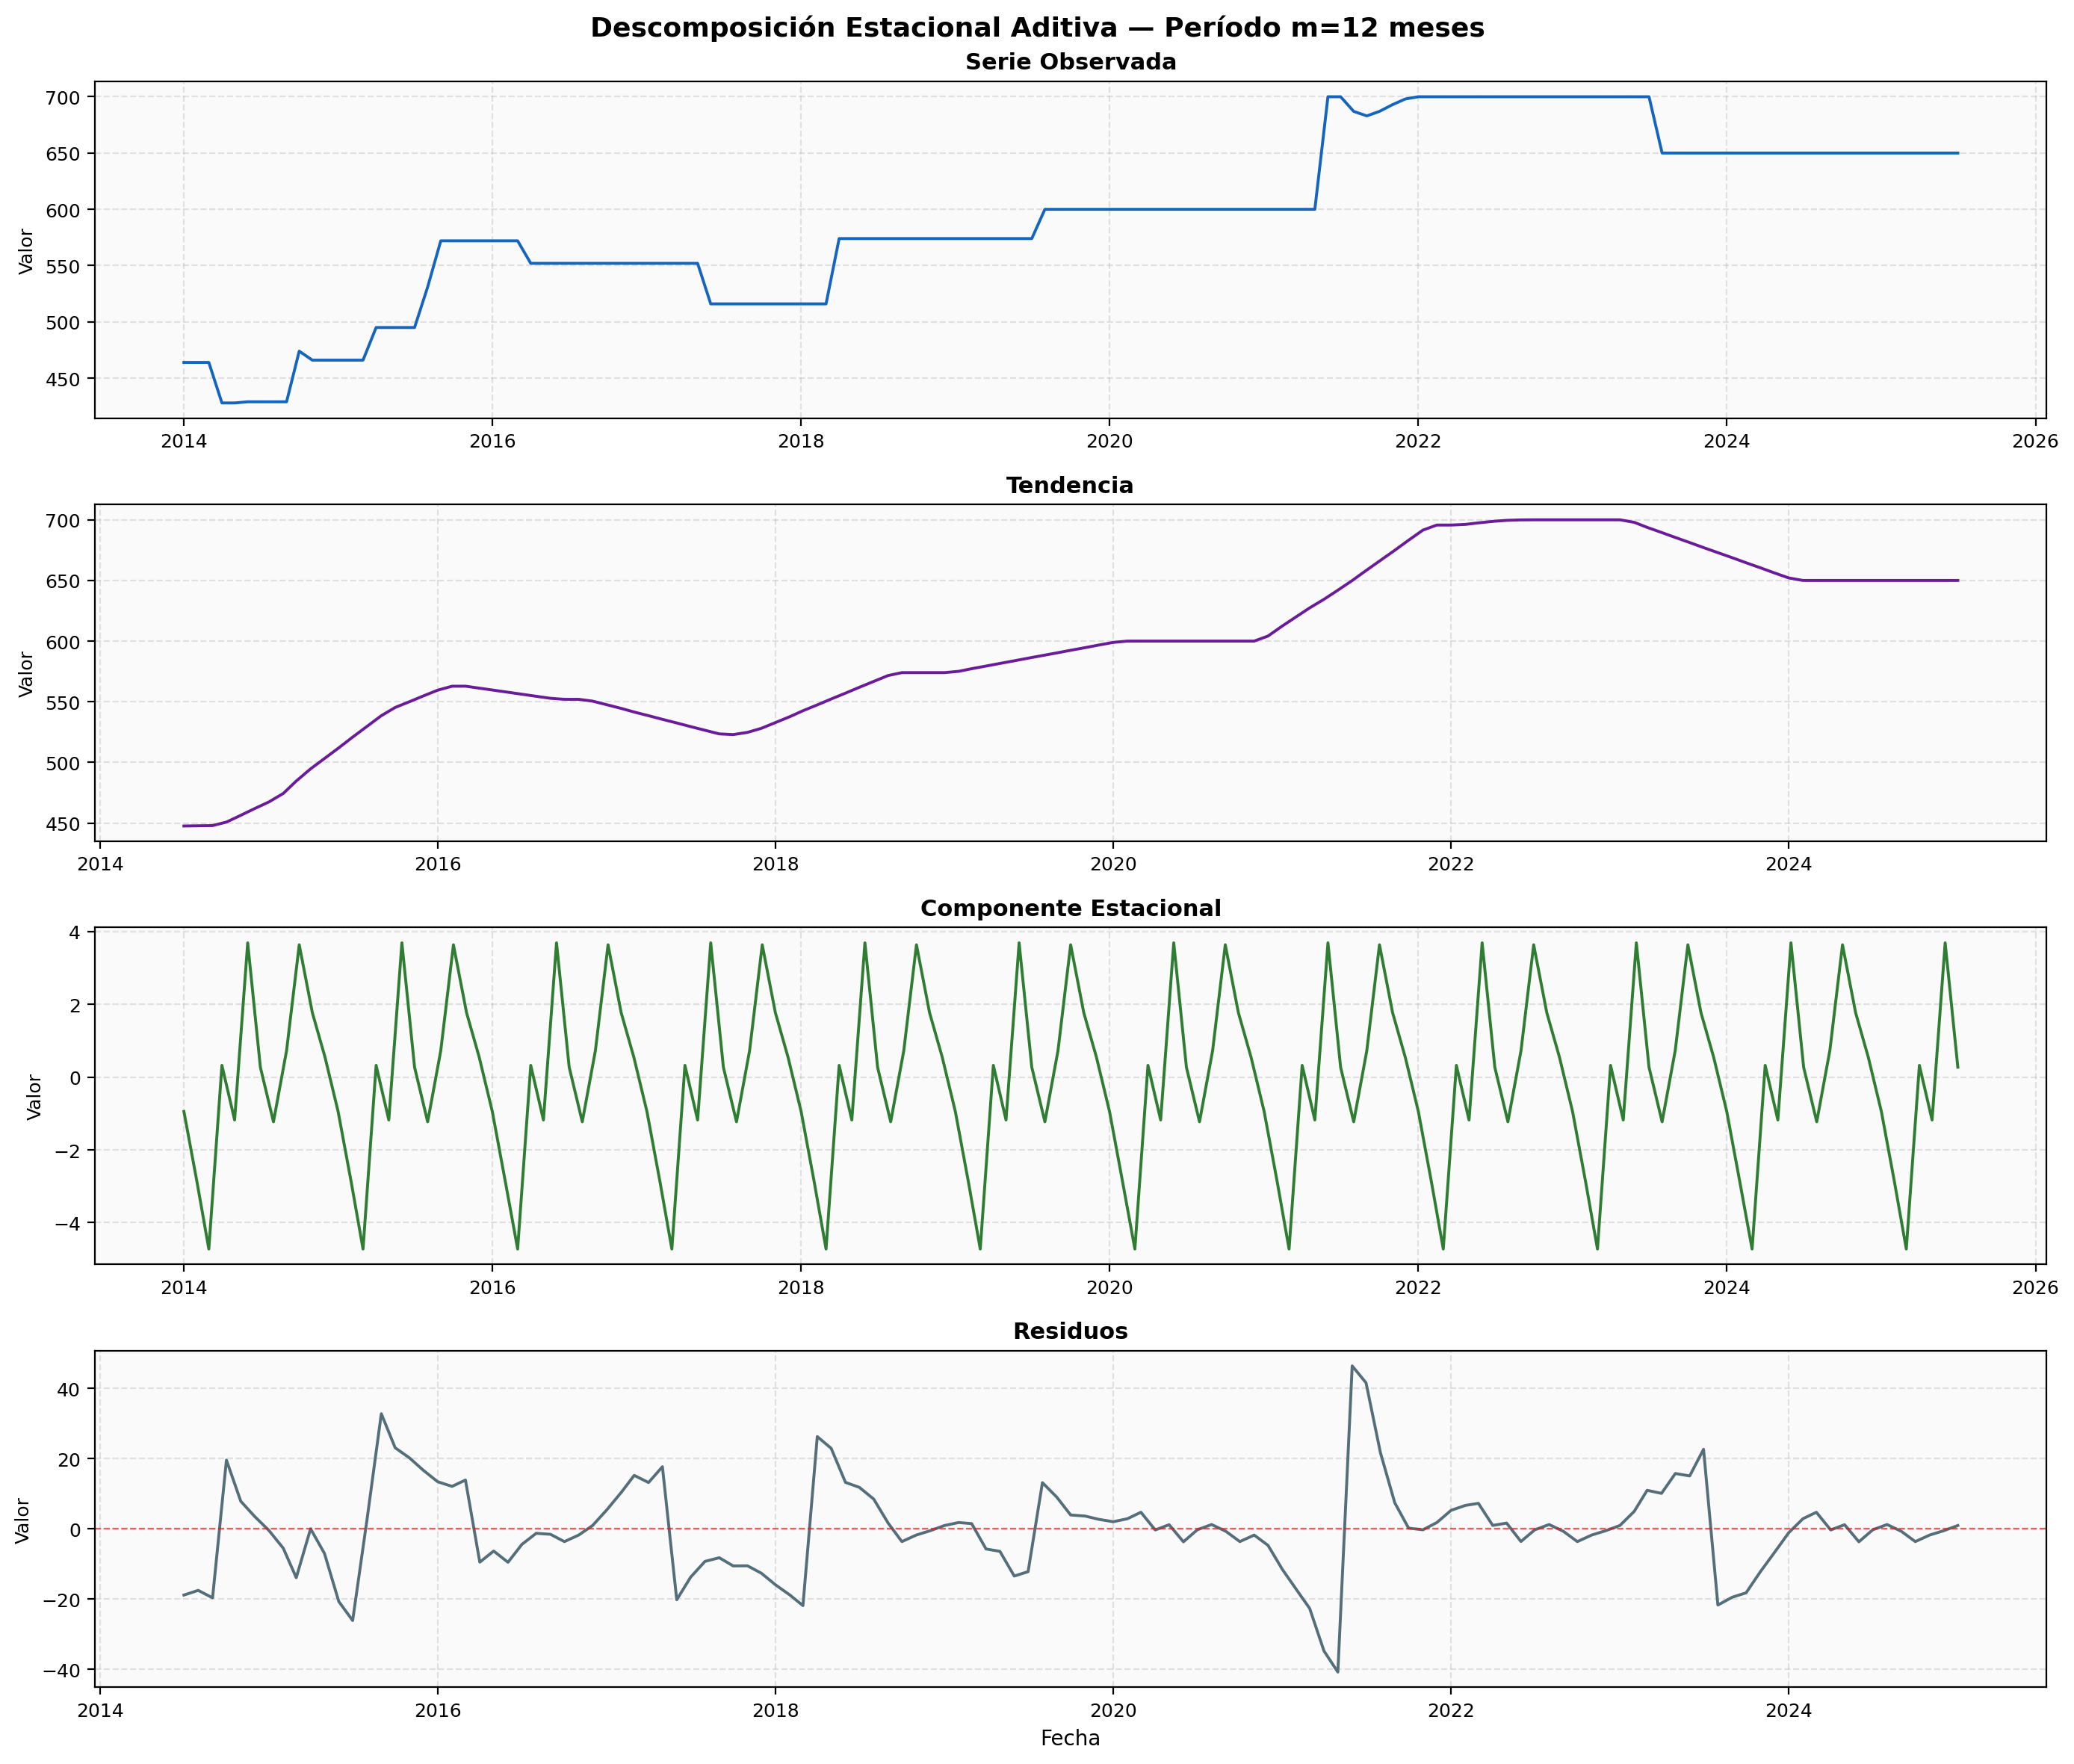
\includegraphics[width=\textwidth]{predicciones/prediccion_sarimax_ladrillo/graficos/02_descomposicion_estacional.png}
    \caption{Descomposición estacional de la serie de precio del ladrillo: tendencia, estacionalidad y componente residual.}
    \label{fig:sarimax_ladrillo_descomposicion}
\end{figure}

\justify
La Figura \ref{fig:sarimax_ladrillo_descomposicion} presenta la descomposición clásica de la serie del ladrillo. La componente de tendencia confirma el crecimiento sostenido del precio, con una aceleración a partir de 2020. La componente estacional muestra patrones de amplitud moderada con período anual, y los residuos no evidencian estructura sistemática.

\begin{figure}[ht]
    \centering
    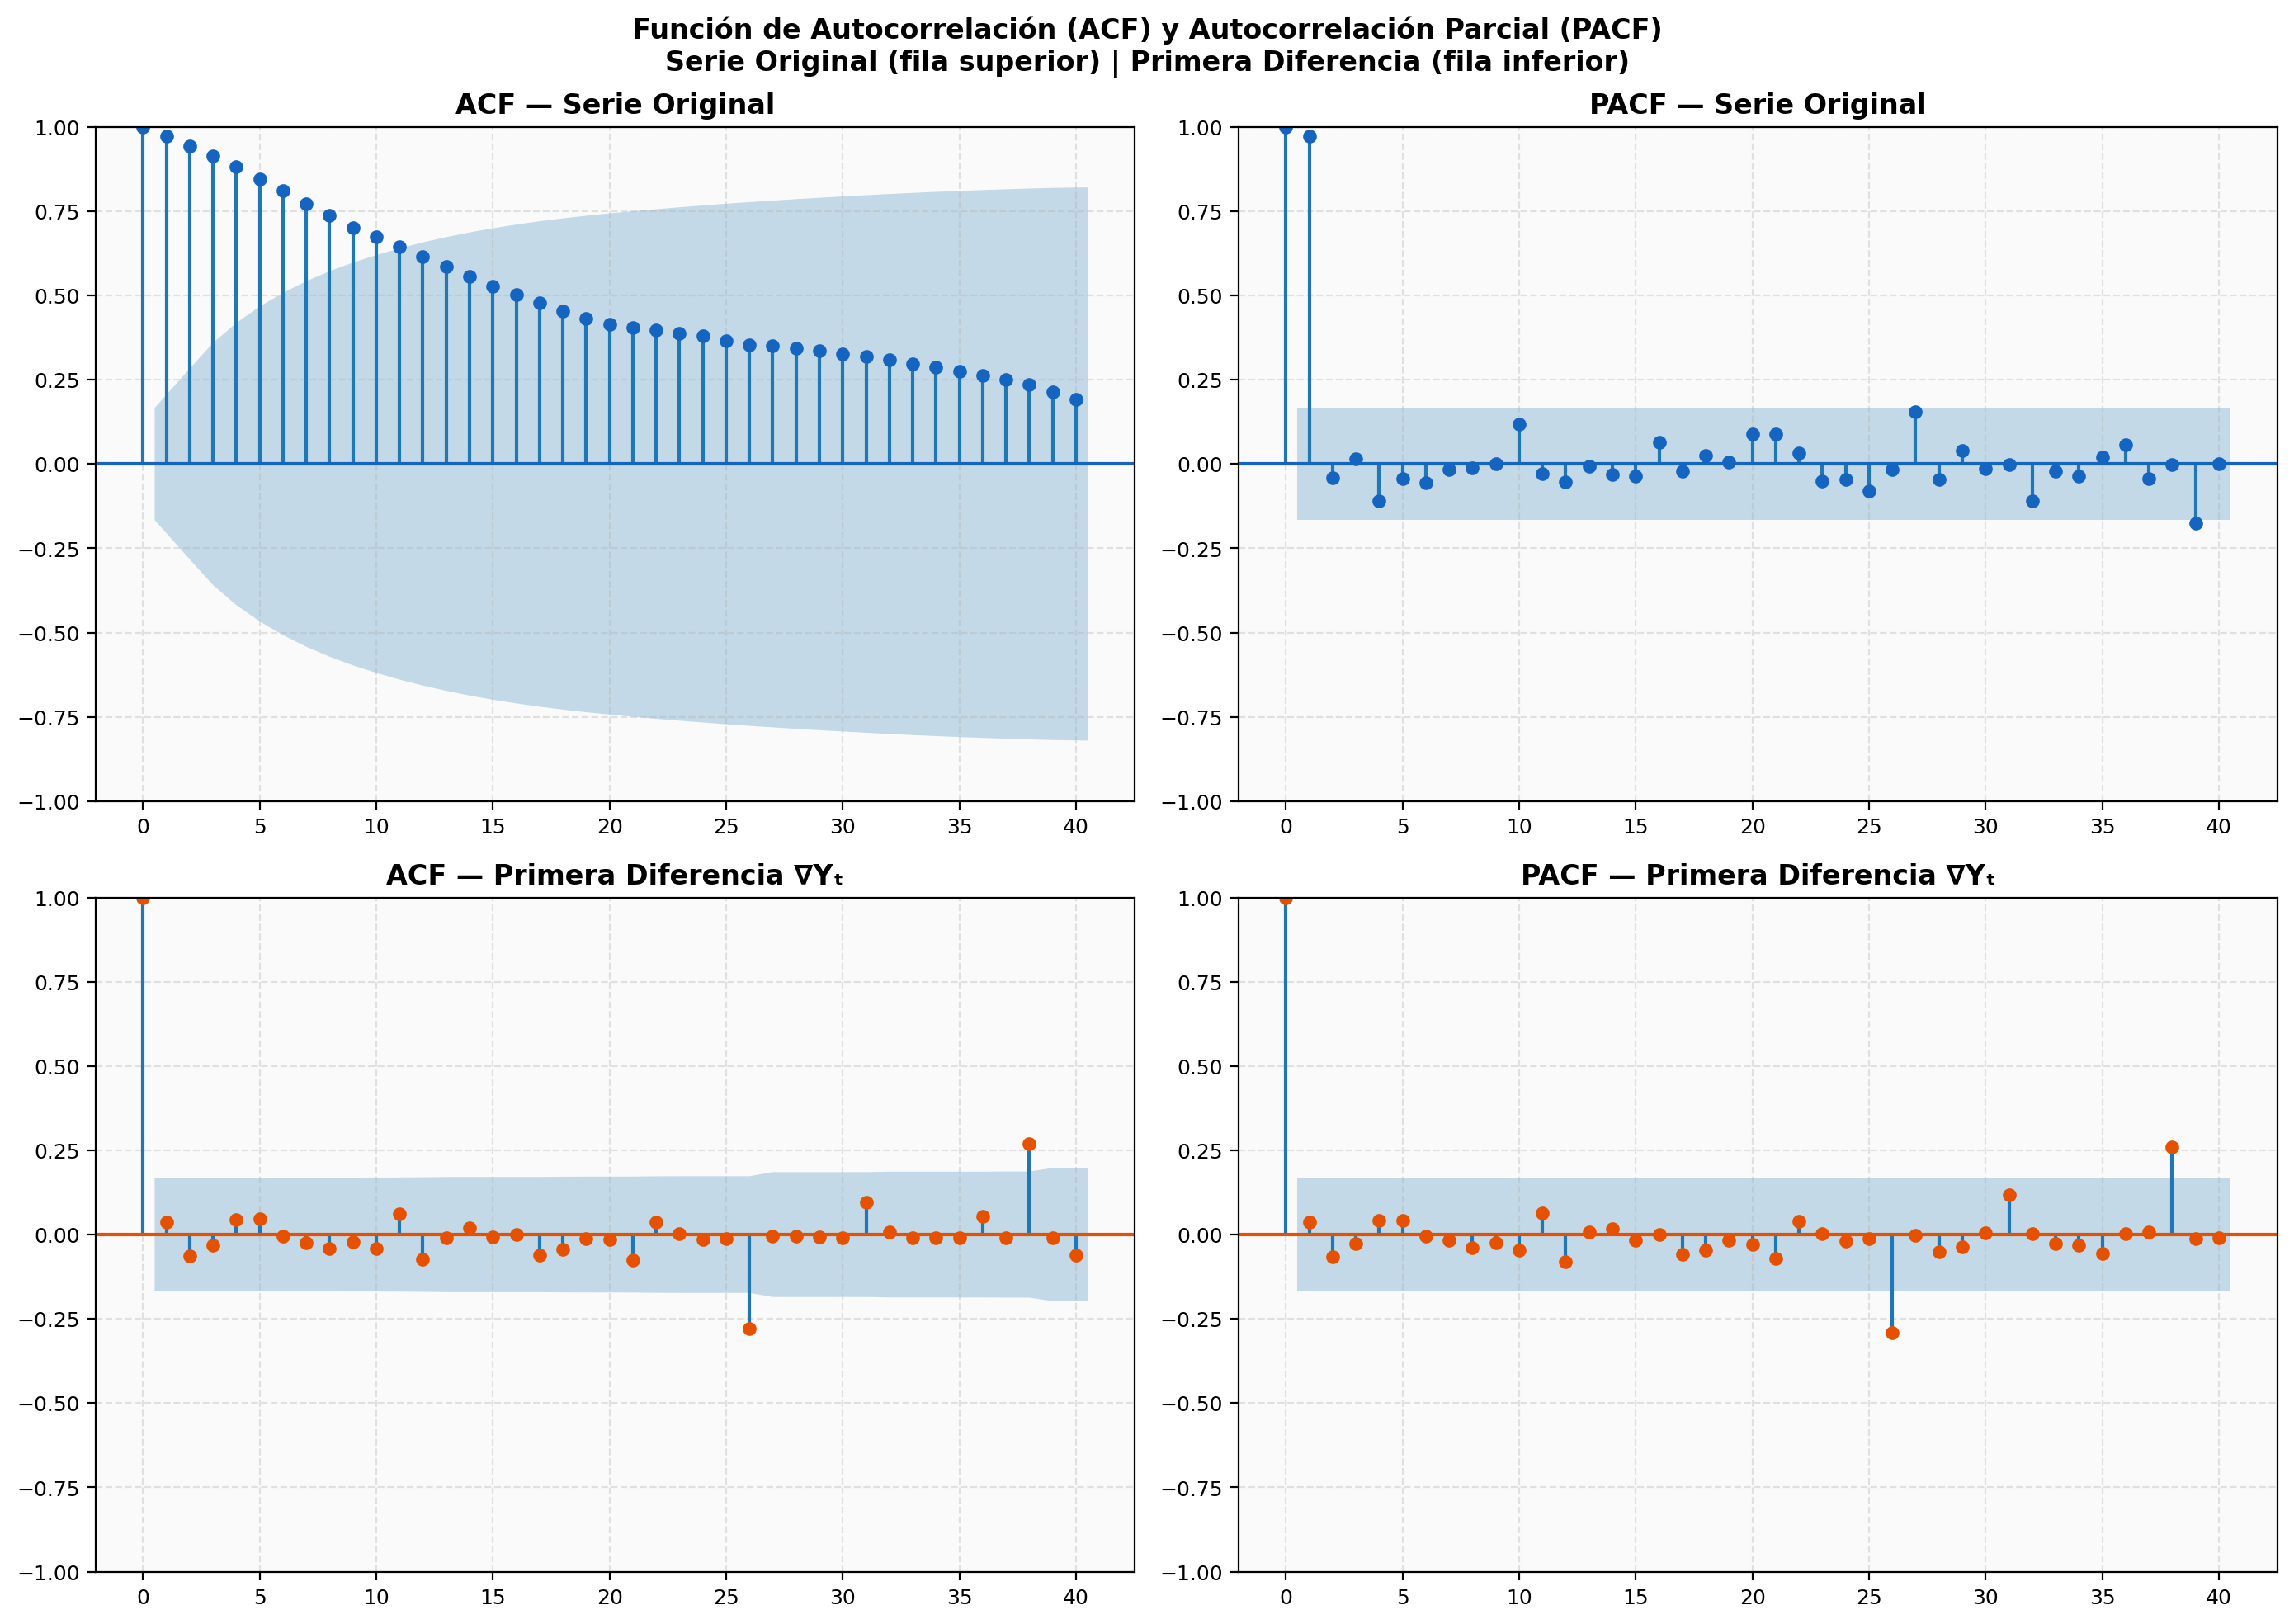
\includegraphics[width=\textwidth]{predicciones/prediccion_sarimax_ladrillo/graficos/03_acf_pacf.png}
    \caption{Funciones de autocorrelación (ACF) y autocorrelación parcial (PACF) de la serie del precio del ladrillo en niveles y en primeras diferencias.}
    \label{fig:sarimax_ladrillo_acf_pacf}
\end{figure}

\justify
La Figura \ref{fig:sarimax_ladrillo_acf_pacf} muestra las funciones ACF y PACF de la serie original y de su primera diferencia. Al igual que en el caso del cemento, la serie en niveles presenta una ACF con decaimiento lento, indicando no estacionariedad. Tras la primera diferencia, la ACF decae hacia cero, justificando el orden de integración $d=1$.

\begin{figure}[ht]
    \centering
    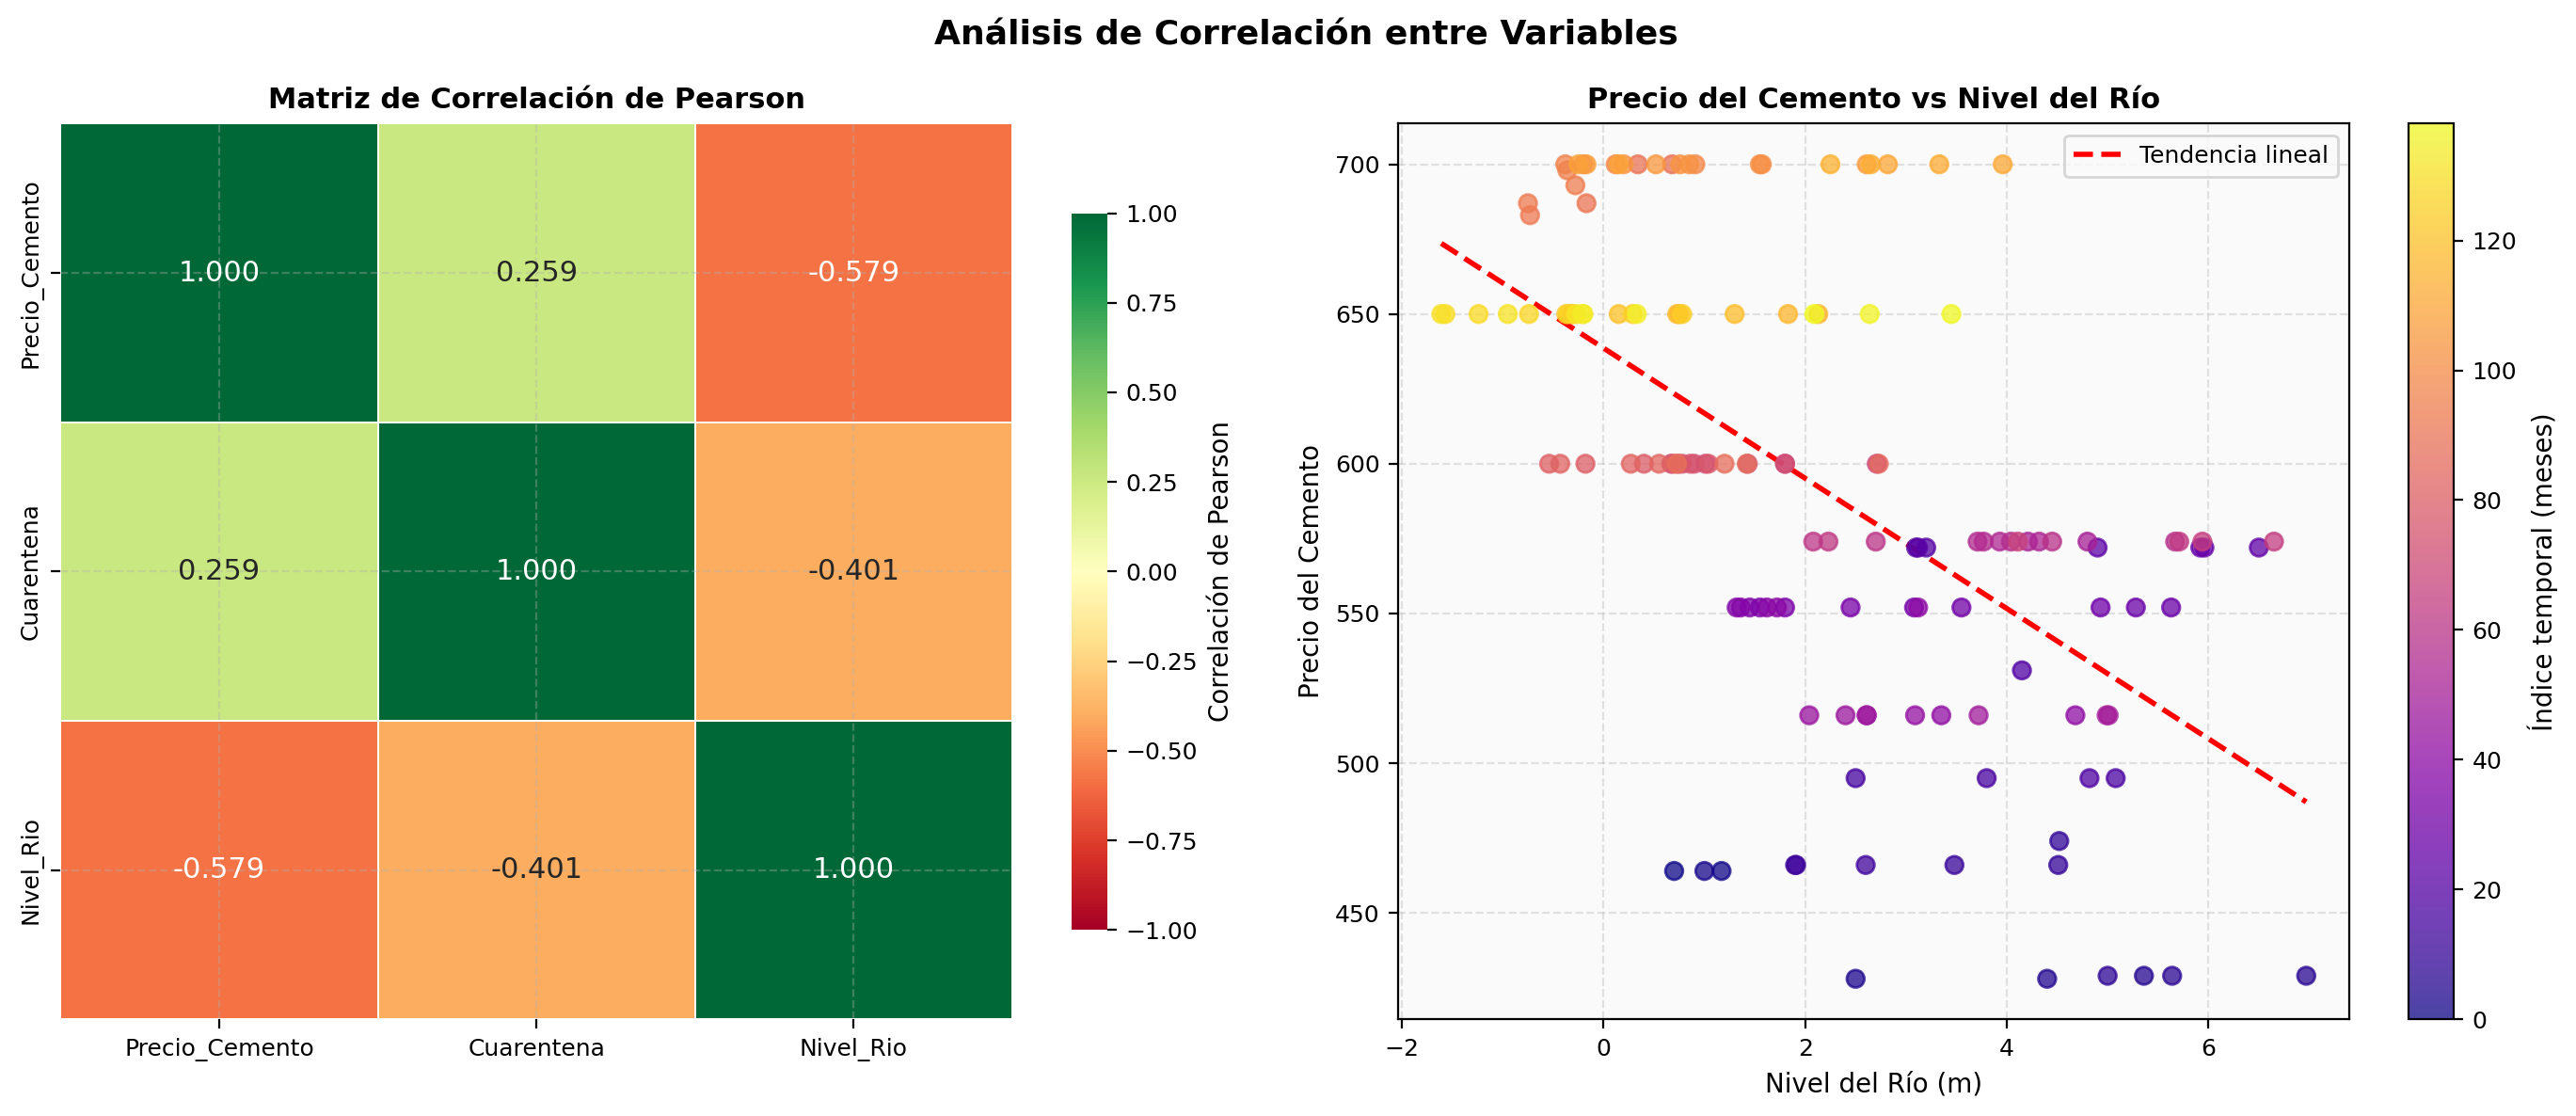
\includegraphics[width=0.8\textwidth]{predicciones/prediccion_sarimax_ladrillo/graficos/04_correlacion.png}
    \caption{Matriz de correlación entre el precio del ladrillo, el nivel del río Paraguay y la variable de cuarentena.}
    \label{fig:sarimax_ladrillo_correlacion}
\end{figure}

\justify
La Figura \ref{fig:sarimax_ladrillo_correlacion} muestra la matriz de correlación entre las variables del modelo. La correlación entre el precio del ladrillo y el nivel del río es de magnitud moderada y negativa, coherente con los resultados obtenidos para el cemento y con la hipótesis logística que sustenta la inclusión de esta variable exógena.

\begin{figure}[ht]
    \centering
    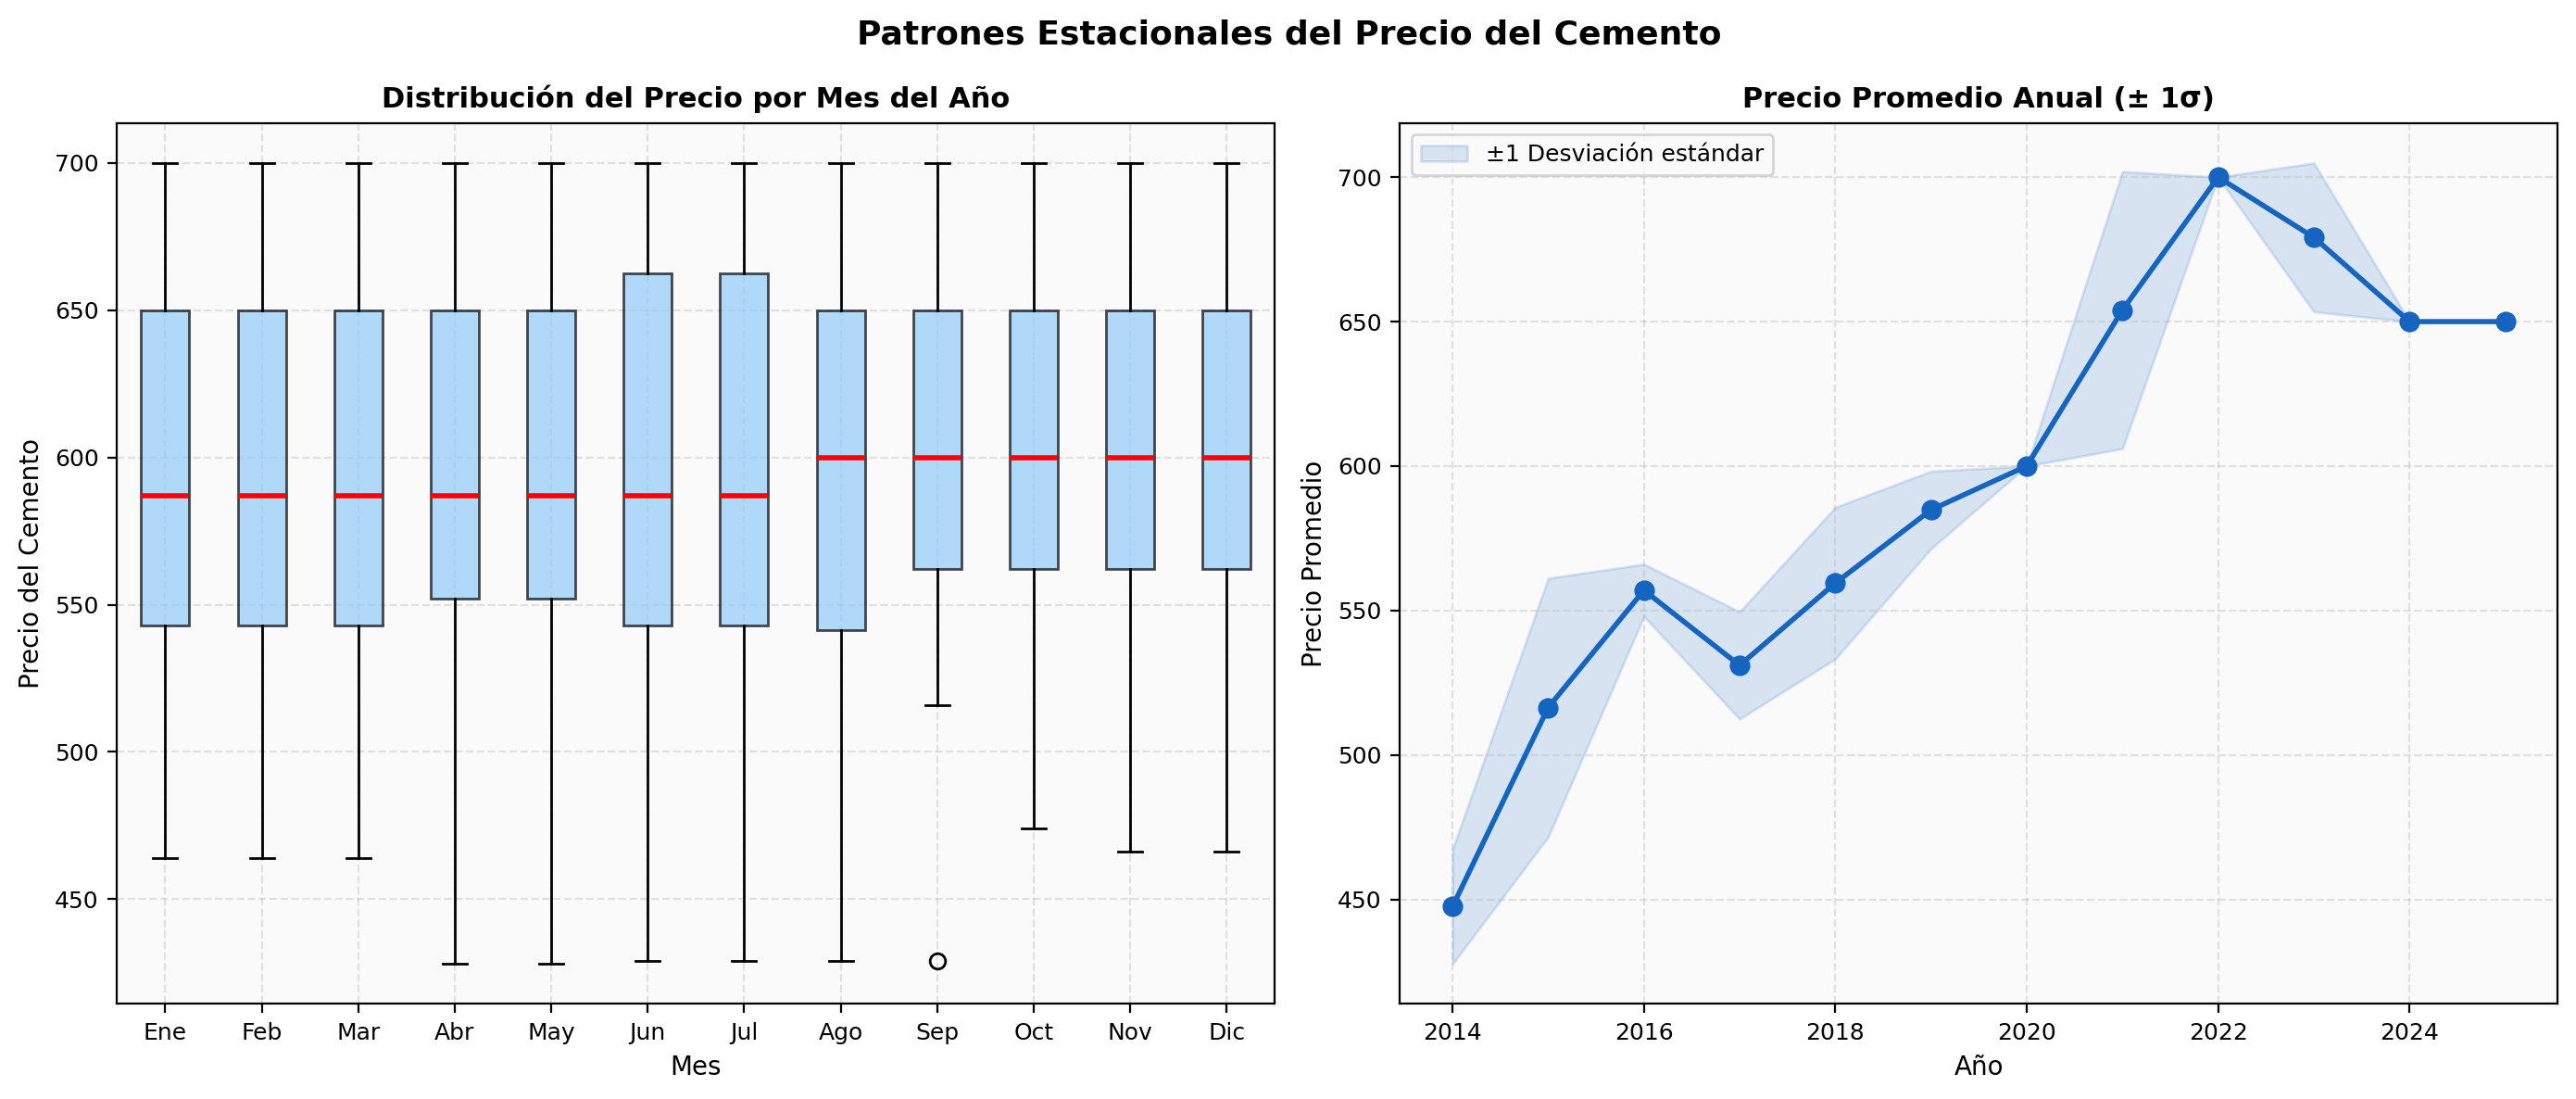
\includegraphics[width=\textwidth]{predicciones/prediccion_sarimax_ladrillo/graficos/05_patron_estacional.png}
    \caption{Patrón estacional del precio mensual del ladrillo a lo largo del año.}
    \label{fig:sarimax_ladrillo_estacional}
\end{figure}

\justify
La Figura \ref{fig:sarimax_ladrillo_estacional} ilustra el patrón estacional del precio del ladrillo. Se observan variaciones de amplitud moderada, con precios ligeramente superiores en los meses de mayor demanda de la construcción.

\subsubsection{Modelo SARIMAX: Selección y Parámetros}

\justify
La selección del orden óptimo del modelo SARIMAX se realizó mediante búsqueda exhaustiva sobre el espacio de parámetros $(p, d, q) \times (P, D, Q)_{12}$, minimizando el AIC. El modelo seleccionado corresponde al orden SARIMAX$(0,1,0)(0,0,0)_{12}$, coincidiendo con el resultado obtenido para el cemento, con un AIC de 1109{,}56 y un BIC de 1118{,}32.

\justify
Los parámetros estimados del modelo se resumen en la Tabla \ref{tab:sarimax_ladrillo_params}. El coeficiente asociado al nivel del río (\texttt{Nivel\_Rio}) resultó negativo ($-1{,}93$~Gs./m) y estadísticamente no significativo ($p=0{,}302$). La variable \texttt{Cuarentena} tampoco alcanzó significancia estadística ($p=0{,}999$), comportamiento análogo al observado en el modelo del cemento.

\begin{table}[ht]
    \centering
    \caption{Parámetros estimados del modelo SARIMAX$(0,1,0)(0,0,0)_{12}$ para la predicción del precio del ladrillo.}
    \label{tab:sarimax_ladrillo_params}
    \begin{tabular}{lrrrr}
        \toprule
        \textbf{Parámetro} & \textbf{Coeficiente} & \textbf{Error est.} & \textbf{z} & \textbf{p-valor} \\
        \midrule
        \texttt{Nivel\_Rio}  & $-1{,}931$ & $1{,}873$ & $-1{,}031$ & $0{,}302$ \\
        \texttt{Cuarentena}  & $-0{,}819$ & $643{,}258$ & $-0{,}001$ & $0{,}999$ \\
        $\sigma^{2}$         & $184{,}44$ & $6{,}384$ & $28{,}890$ & $0{,}000$ \\
        \midrule
        \multicolumn{2}{l}{AIC} & \multicolumn{3}{r}{1109{,}56} \\
        \multicolumn{2}{l}{BIC} & \multicolumn{3}{r}{1118{,}32} \\
        \multicolumn{2}{l}{Log-verosimilitud} & \multicolumn{3}{r}{$-551{,}78$} \\
        \bottomrule
    \end{tabular}
\end{table}

\justify
La coincidencia en el orden del modelo seleccionado ---SARIMAX$(0,1,0)$ tanto para el cemento como para el ladrillo--- sugiere que ambas series de precios comparten una dinámica subyacente similar: en su forma diferenciada, se comportan como ruido blanco con contribución marginal de las variables exógenas. Este resultado es coherente con mercados de insumos de construcción en los que los ajustes de precio son infrecuentes y se mantienen estables durante períodos prolongados.

\subsubsection{Modelo SARIMAX: Ajuste y Evaluación}

\begin{figure}[ht]
    \centering
    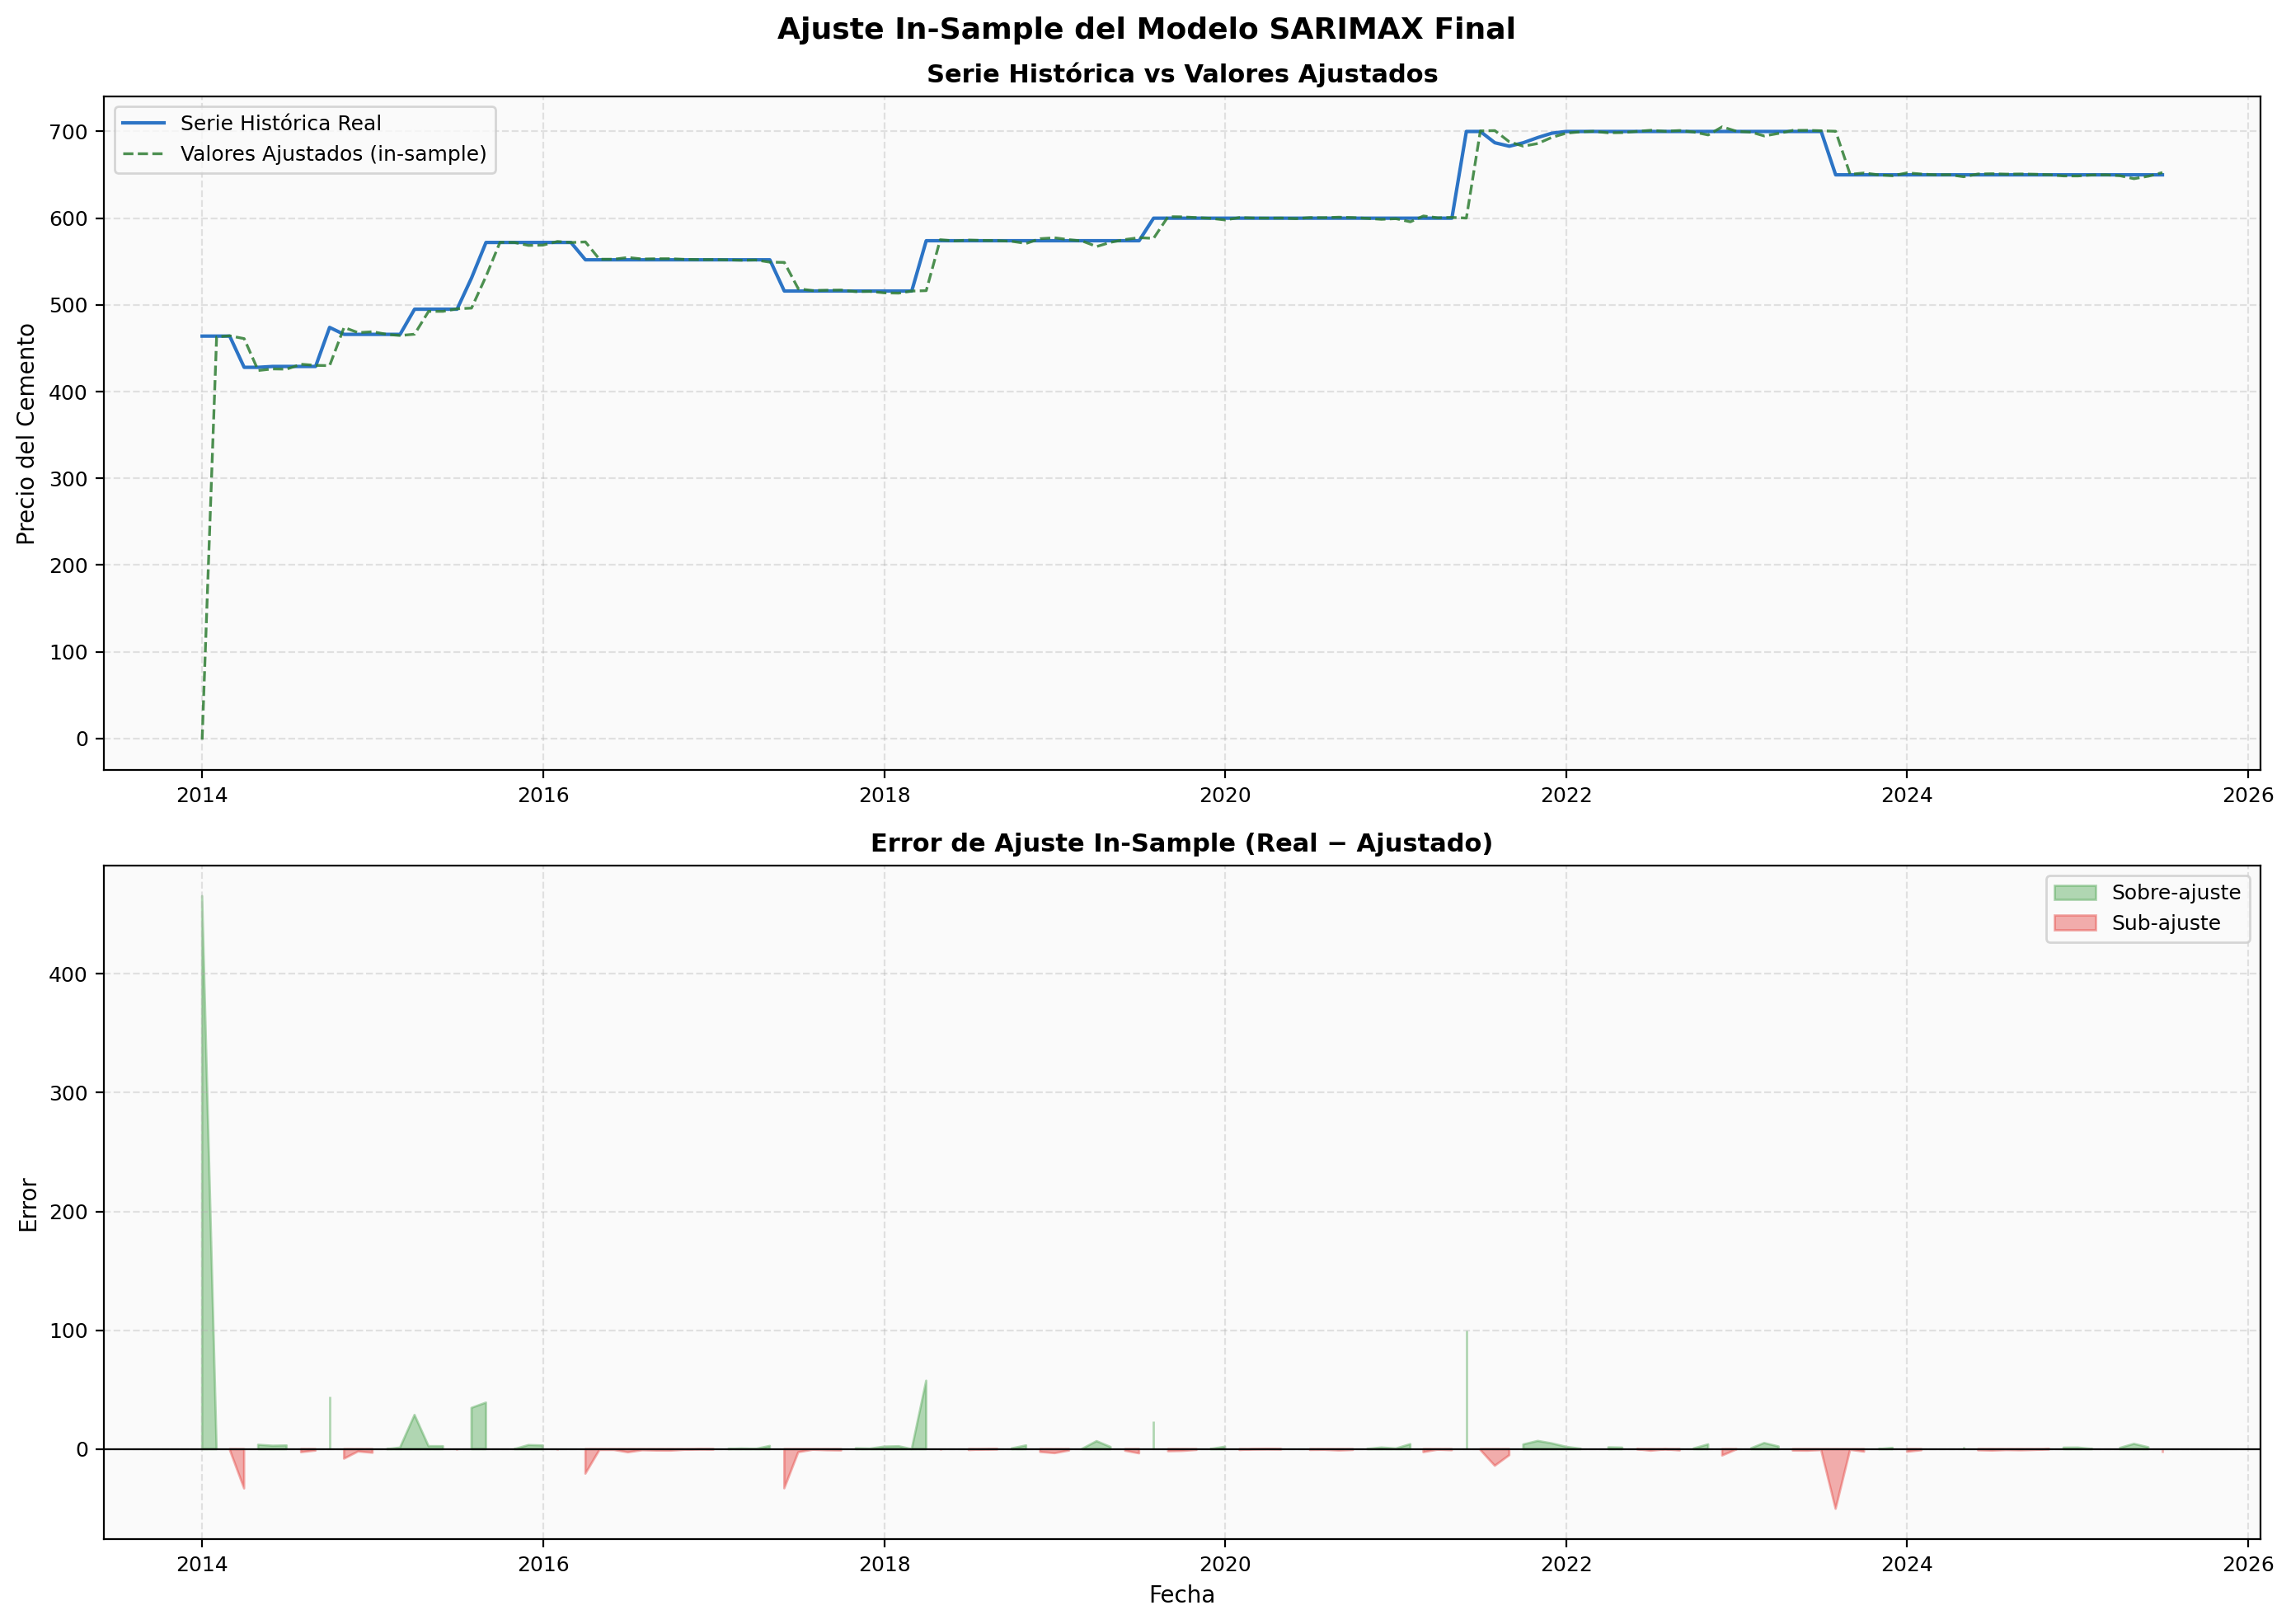
\includegraphics[width=\textwidth]{predicciones/prediccion_sarimax_ladrillo/graficos/11_ajuste_insample.png}
    \caption{Ajuste in-sample del modelo SARIMAX: valores reales versus valores ajustados para el precio del ladrillo.}
    \label{fig:sarimax_ladrillo_insample}
\end{figure}

\justify
La Figura \ref{fig:sarimax_ladrillo_insample} muestra el ajuste del modelo sobre los datos de entrenamiento. El modelo sigue adecuadamente la trayectoria histórica del precio del ladrillo, incluyendo los incrementos escalonados registrados a lo largo del período.

\begin{figure}[ht]
    \centering
    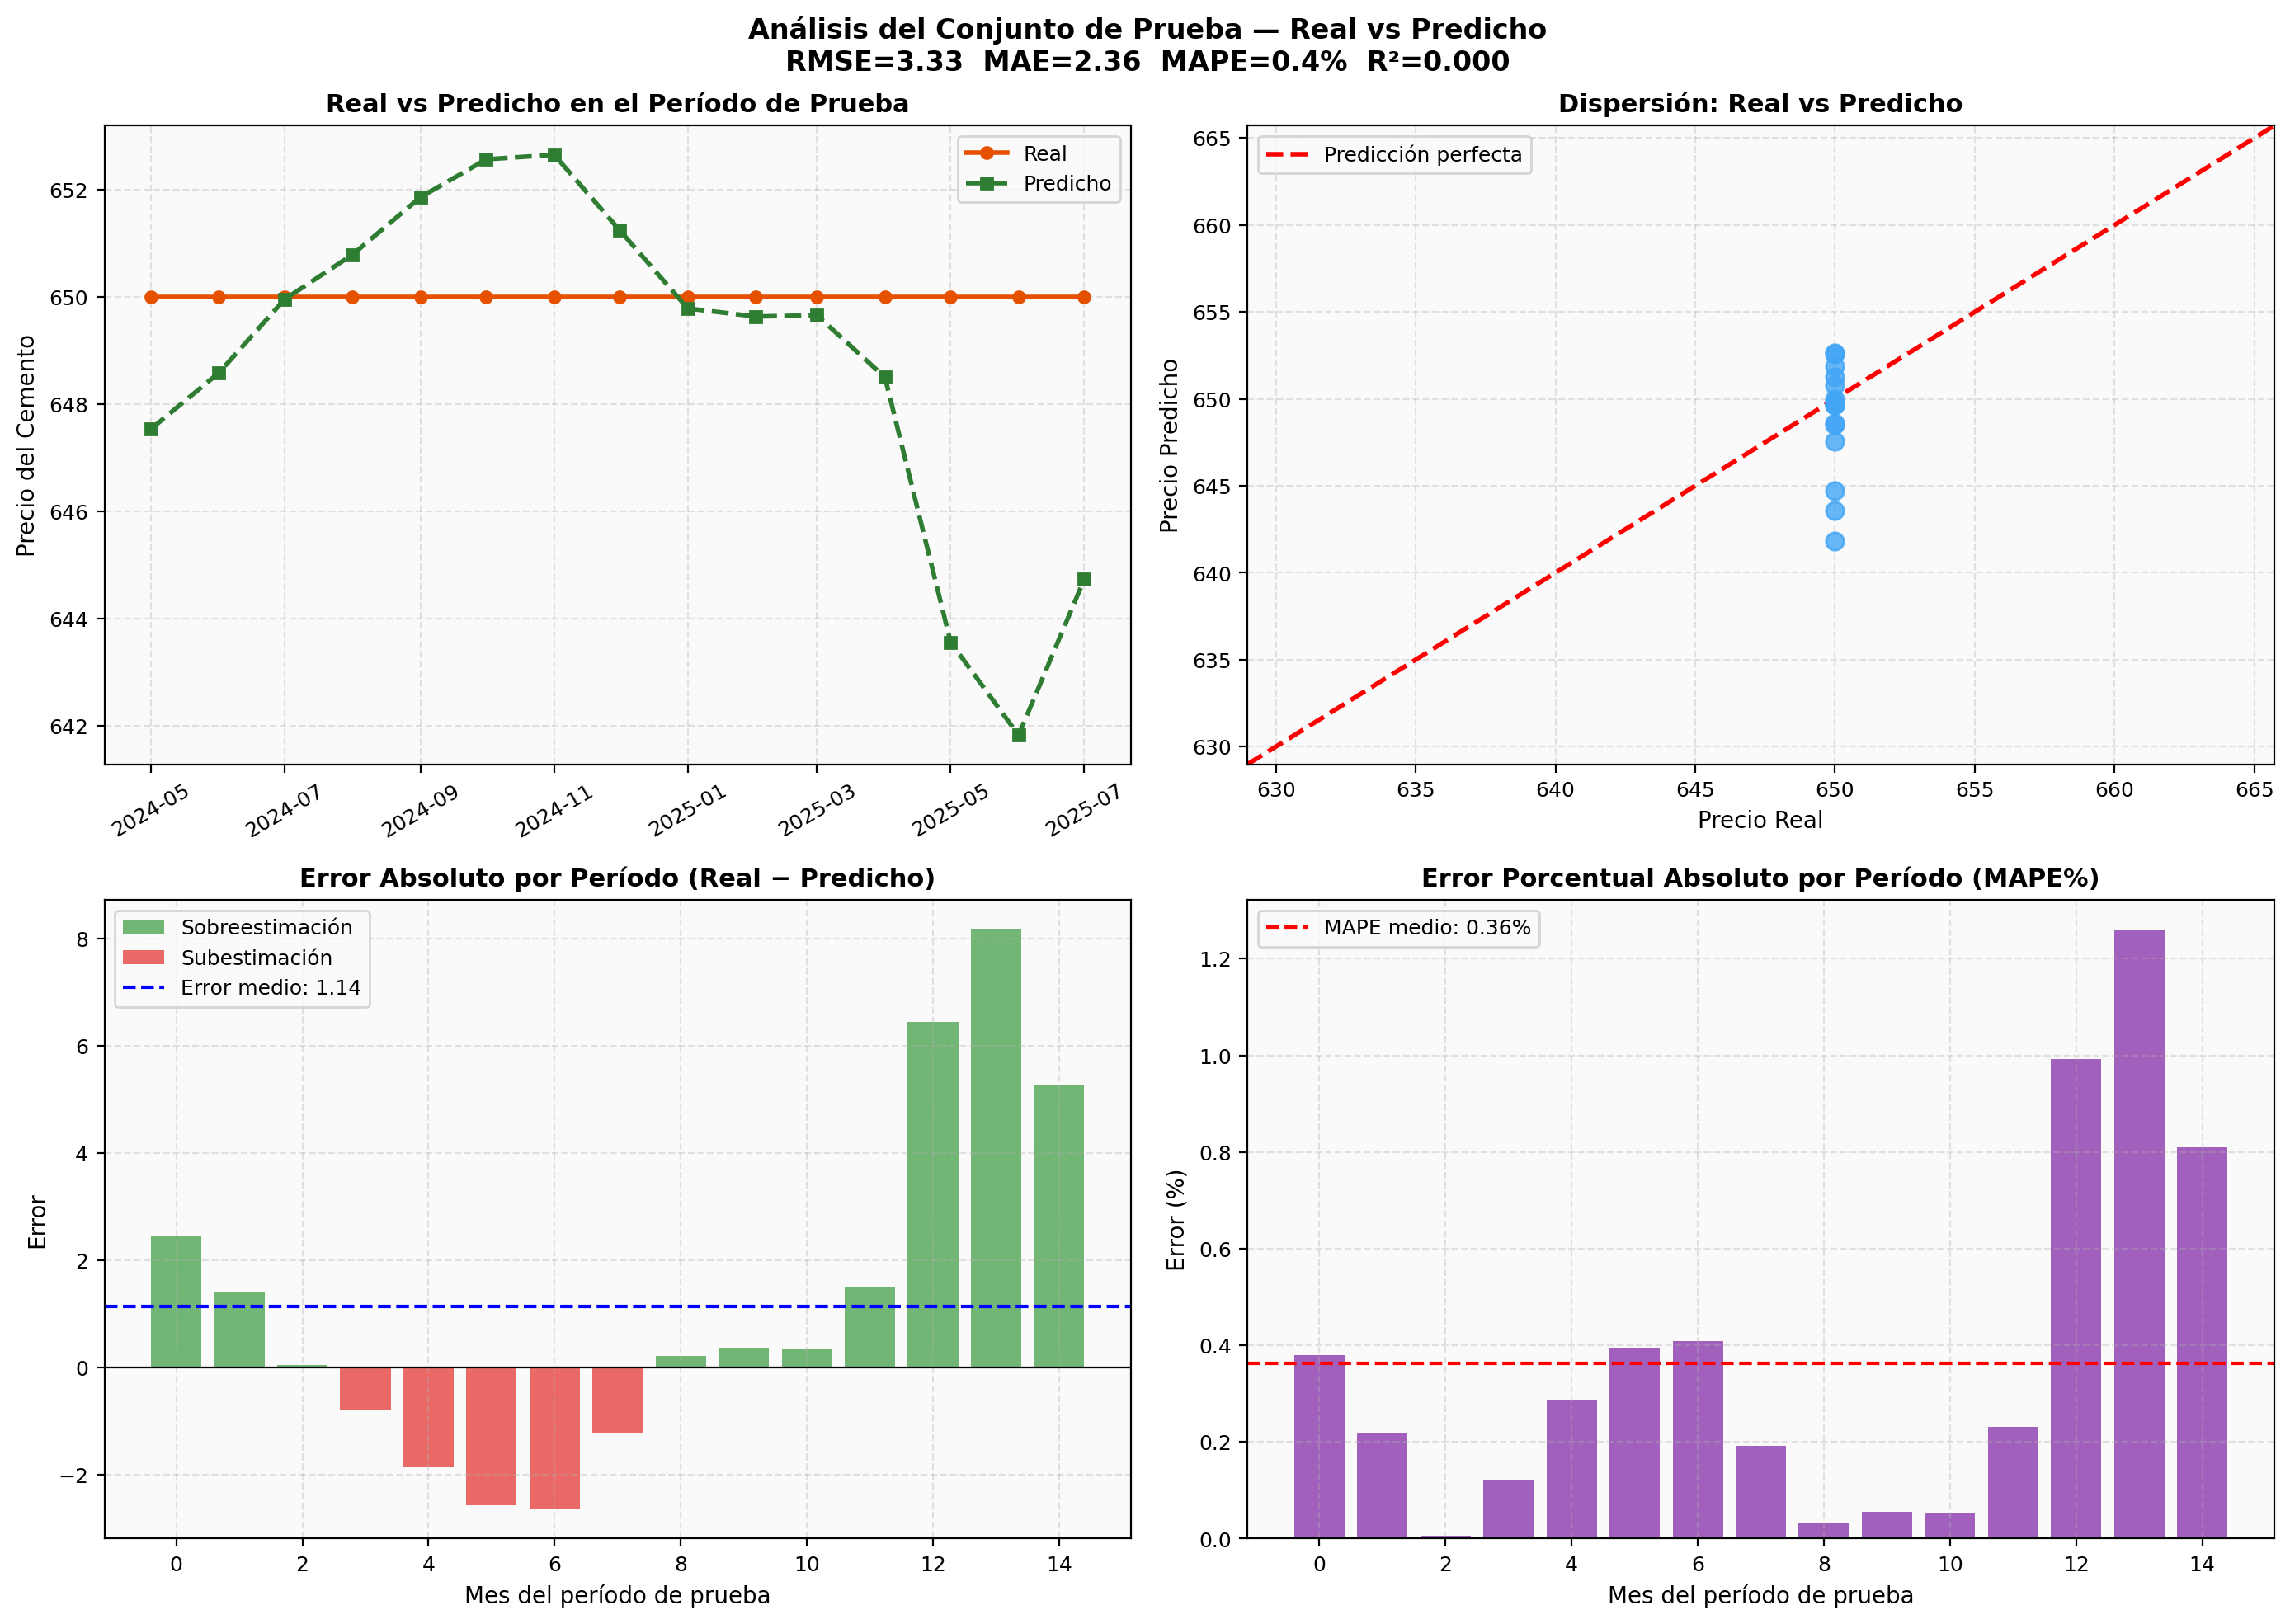
\includegraphics[width=\textwidth]{predicciones/prediccion_sarimax_ladrillo/graficos/08_comparacion_real_predicho.png}
    \caption{Comparación entre los valores reales y predichos del precio del ladrillo en el conjunto de prueba (15 meses).}
    \label{fig:sarimax_ladrillo_comparacion}
\end{figure}

\justify
La Figura \ref{fig:sarimax_ladrillo_comparacion} presenta la comparación entre los valores reales y los predichos por el modelo sobre el conjunto de prueba de 15 meses. Las métricas de evaluación se resumen en la Tabla \ref{tab:sarimax_ladrillo_metricas_prueba}.

\begin{table}[ht]
    \centering
    \caption{Métricas de evaluación del modelo SARIMAX sobre el conjunto de prueba del ladrillo (15 meses).}
    \label{tab:sarimax_ladrillo_metricas_prueba}
    \begin{tabular}{lc}
        \toprule
        \textbf{Métrica} & \textbf{Valor} \\
        \midrule
        RMSE (Raíz del Error Cuadrático Medio) & 3{,}33~Gs. \\
        MAE  (Error Absoluto Medio)            & 2{,}36~Gs. \\
        MAPE (Error Porcentual Medio Absoluto) & 0{,}36\,\% \\
        SMAPE (Error Porcentual Simétrico)     & 0{,}36\,\% \\
        Error Absoluto Máximo                  & 8{,}18~Gs. \\
        $R^{2}$ (Coeficiente de Determinación) & 0{,}0000 \\
        \bottomrule
    \end{tabular}
\end{table}

\justify
Al igual que en el caso del cemento, el MAPE de 0{,}36\,\% indica predicciones puntuales con un error relativo muy bajo, pero el $R^{2}=0$ refleja que durante el período de prueba el precio del ladrillo se mantuvo prácticamente estable, de modo que el modelo no puede diferenciarse de una predicción constante en términos de varianza explicada. El patrón es consistente con la naturaleza del modelo $(0,1,0)$: el pronóstico corresponde al último valor observado ajustado por las variables exógenas.

\subsubsection{Modelo SARIMAX: Validación Cruzada}

\begin{figure}[ht]
    \centering
    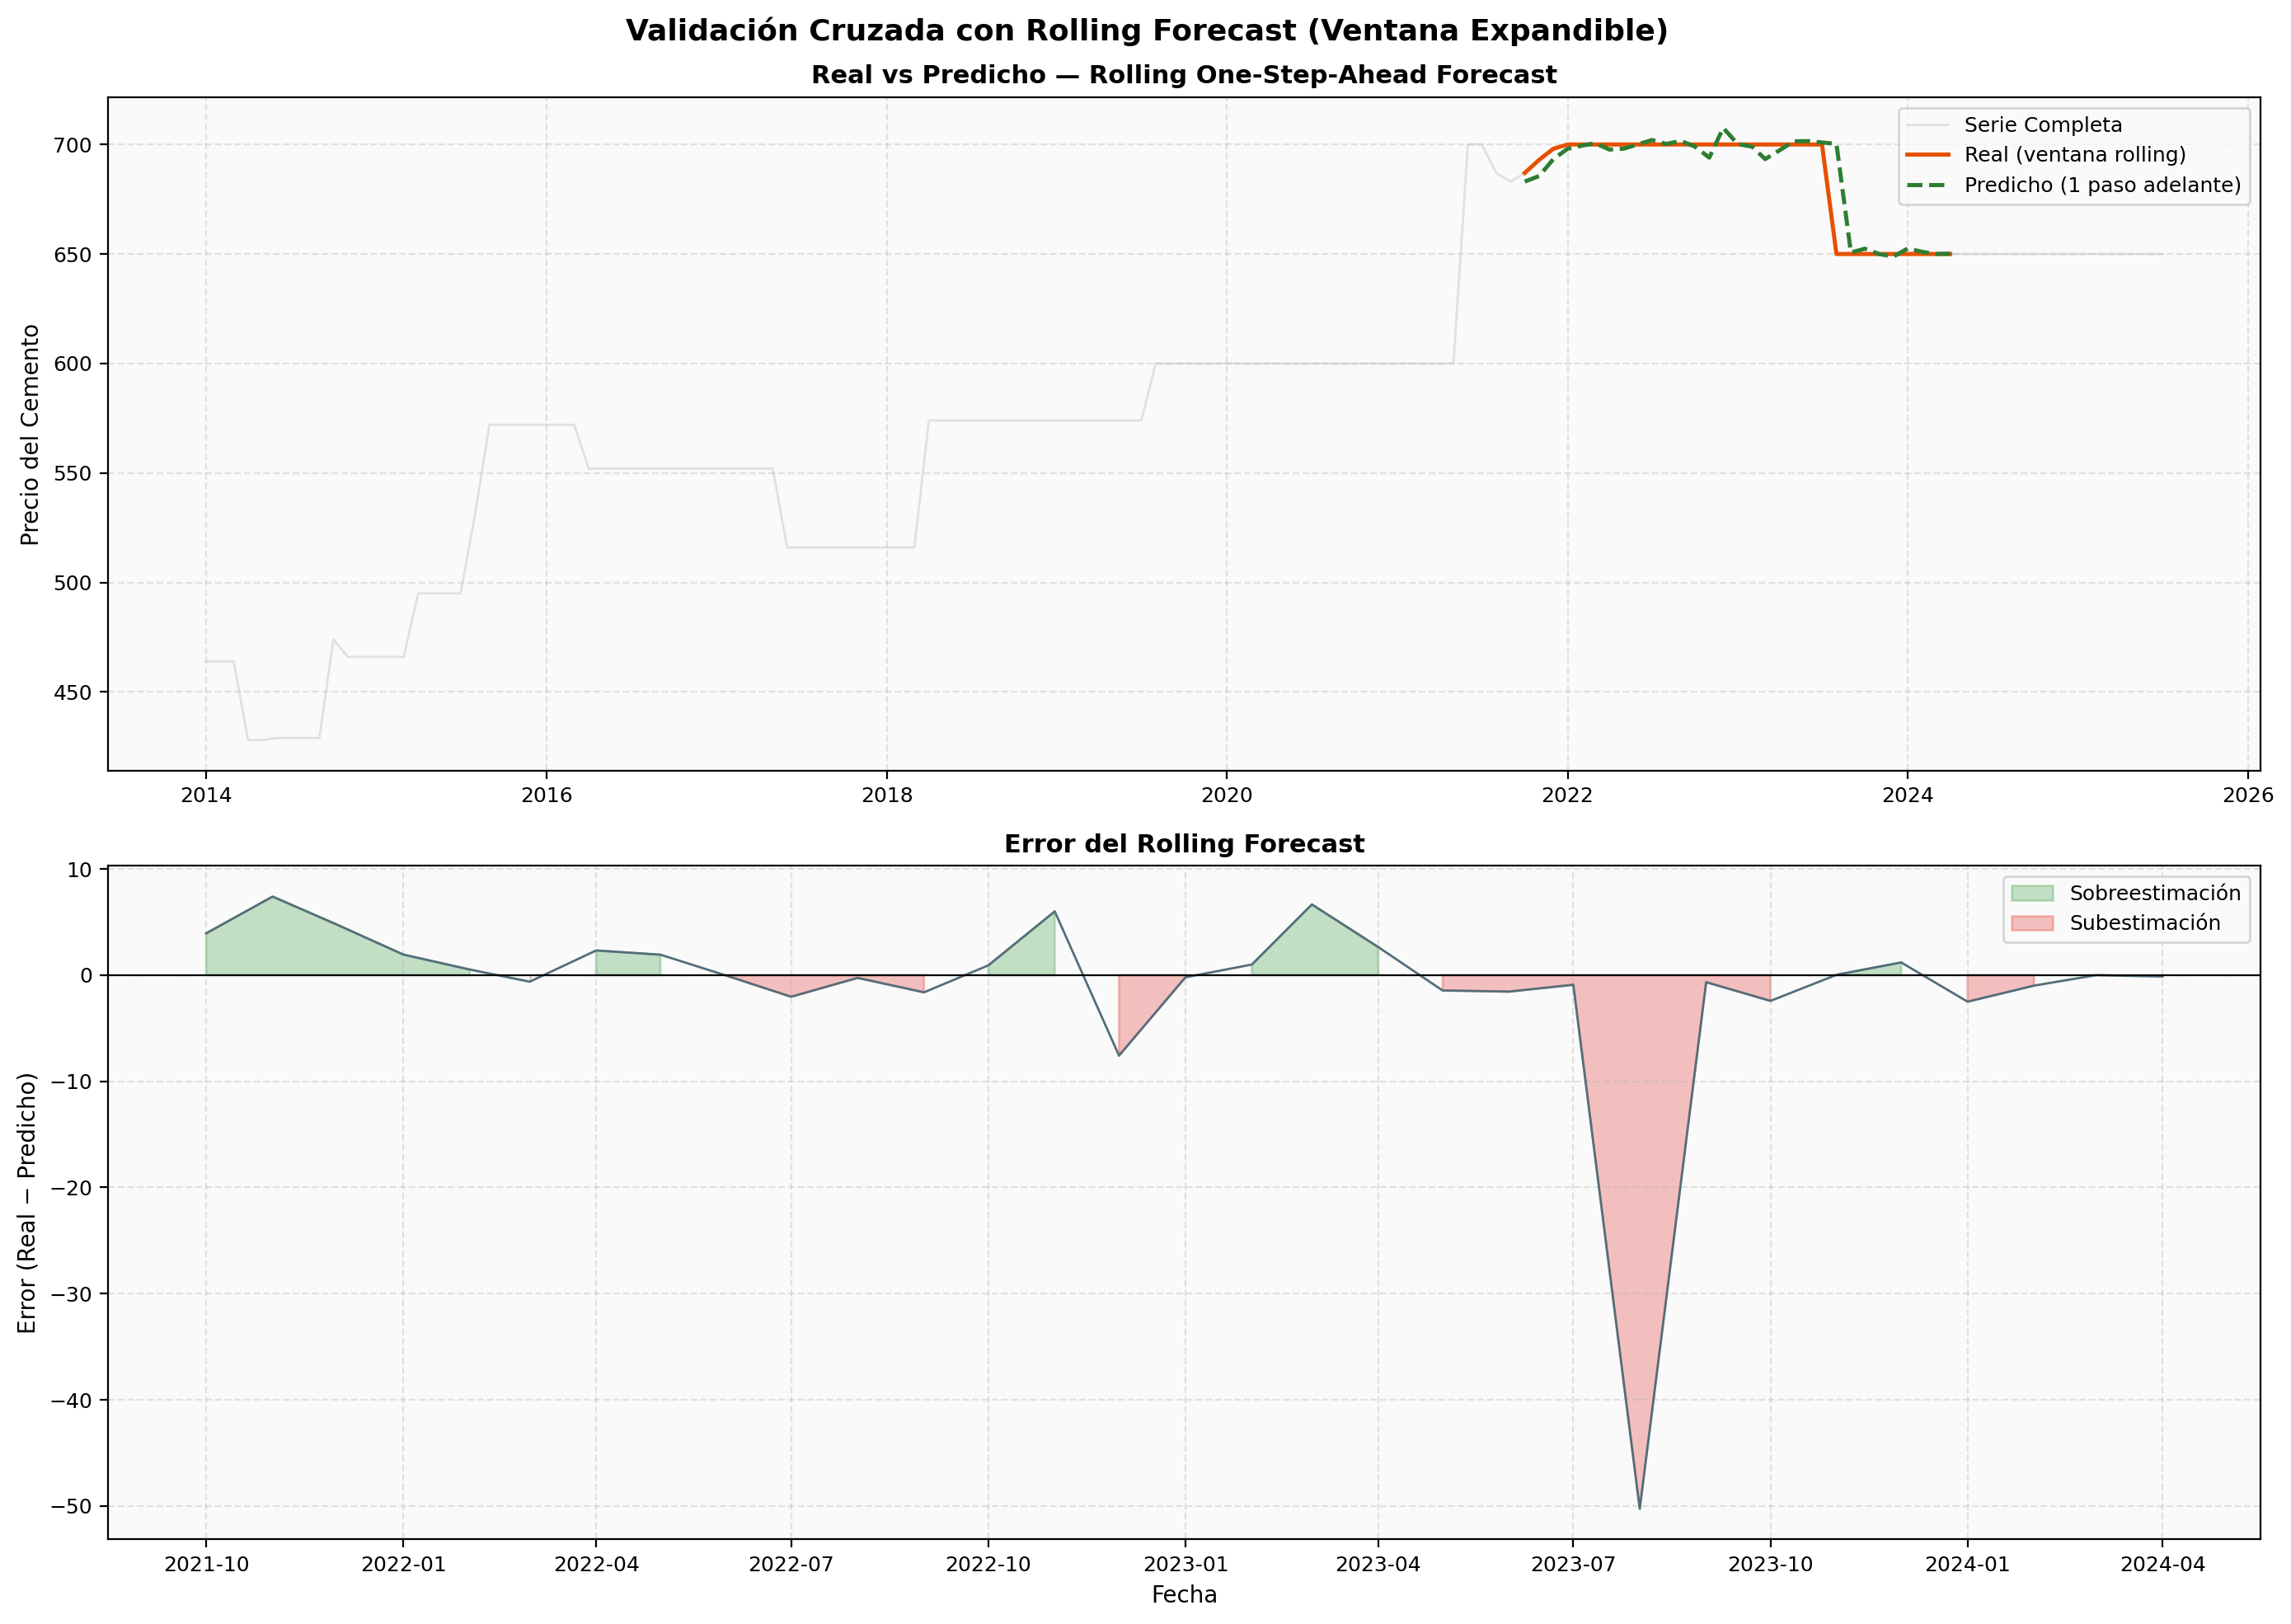
\includegraphics[width=\textwidth]{predicciones/prediccion_sarimax_ladrillo/graficos/10_rolling_forecast_cv.png}
    \caption{Validación cruzada por ventana deslizante del modelo SARIMAX para el precio del ladrillo.}
    \label{fig:sarimax_ladrillo_rolling}
\end{figure}

\justify
La validación cruzada por ventana deslizante ofrece un panorama más representativo del desempeño del modelo. La Figura \ref{fig:sarimax_ladrillo_rolling} muestra las predicciones un paso adelante a lo largo de todo el período evaluado. Las métricas obtenidas se presentan en la Tabla \ref{tab:sarimax_ladrillo_metricas_cv}.

\begin{table}[ht]
    \centering
    \caption{Métricas de validación cruzada por ventana deslizante del modelo SARIMAX para el ladrillo.}
    \label{tab:sarimax_ladrillo_metricas_cv}
    \begin{tabular}{lc}
        \toprule
        \textbf{Métrica} & \textbf{Valor} \\
        \midrule
        RMSE & 9{,}52~Gs. \\
        MAE  & 3{,}69~Gs. \\
        MAPE & 0{,}55\,\% \\
        $R^{2}$ & 0{,}8193 \\
        \bottomrule
    \end{tabular}
\end{table}

\justify
El $R^{2}=0{,}8193$ indica que el modelo explica el 81{,}93\,\% de la varianza del precio del ladrillo a lo largo del período histórico completo, superando incluso al resultado obtenido para el cemento ($R^{2}=0{,}7586$). El MAPE de 0{,}55\,\%, inferior al umbral del 5\,\% habitual para series de precios de materiales, confirma la utilidad práctica del modelo para la estimación presupuestaria.

\subsubsection{Modelo SARIMAX: Análisis de Residuos}

\begin{figure}[ht]
    \centering
    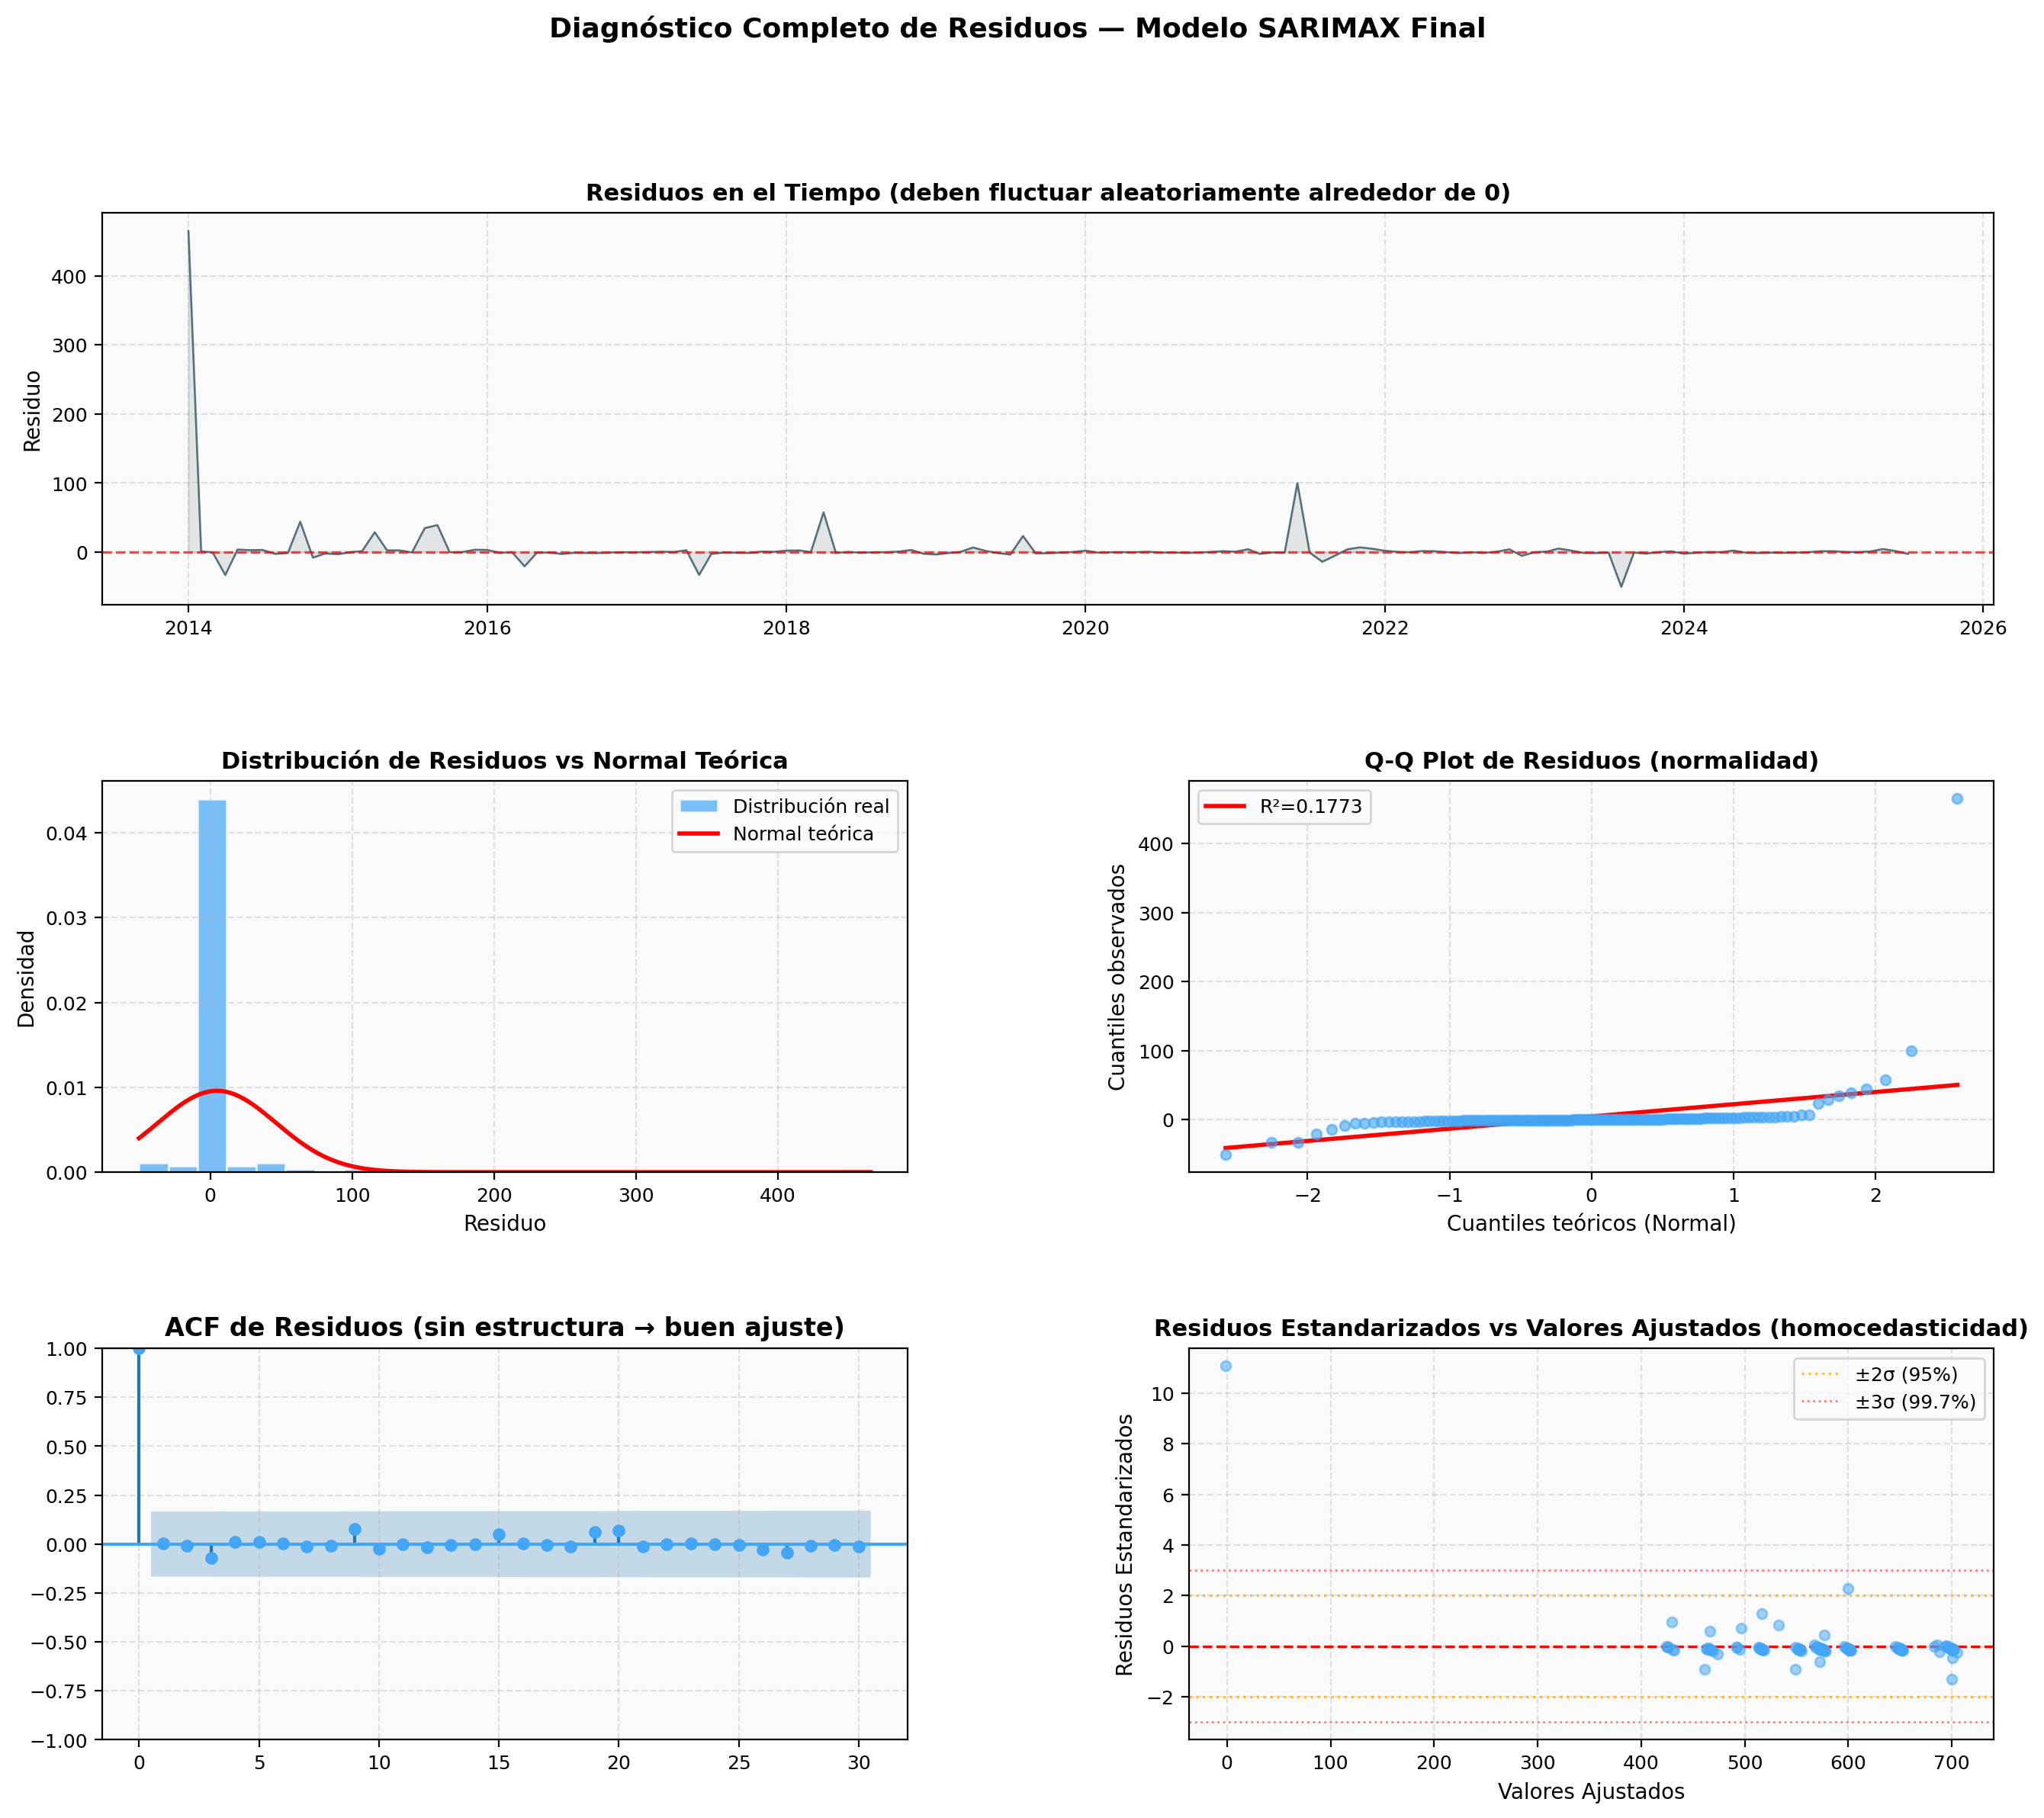
\includegraphics[width=\textwidth]{predicciones/prediccion_sarimax_ladrillo/graficos/07_diagnostico_residuos.png}
    \caption{Diagnóstico de residuos del modelo SARIMAX para el precio del ladrillo.}
    \label{fig:sarimax_ladrillo_residuos}
\end{figure}

\justify
La Figura \ref{fig:sarimax_ladrillo_residuos} presenta el diagnóstico de los residuos. El test de Ljung-Box no rechaza la hipótesis nula de ausencia de autocorrelación serial para los rezagos 10 ($Q=1{,}80$, $p=0{,}998$) y 20 ($Q=3{,}72$, $p=1{,}000$), confirmando que los residuos se comportan como ruido blanco. El test de Shapiro-Wilk rechaza la normalidad ($W=0{,}1936$, $p<0{,}001$), resultado atribuible a la presencia de observaciones extremas que introducen una curtosis de 26{,}69 y una asimetría de 3{,}25. Al igual que en el modelo del cemento, esta no normalidad no invalida las estimaciones puntuales pero impone cautela en la interpretación de los intervalos de confianza.

\subsubsection{Modelo SARIMAX: Pronóstico a 24 Meses}

\begin{figure}[ht]
    \centering
    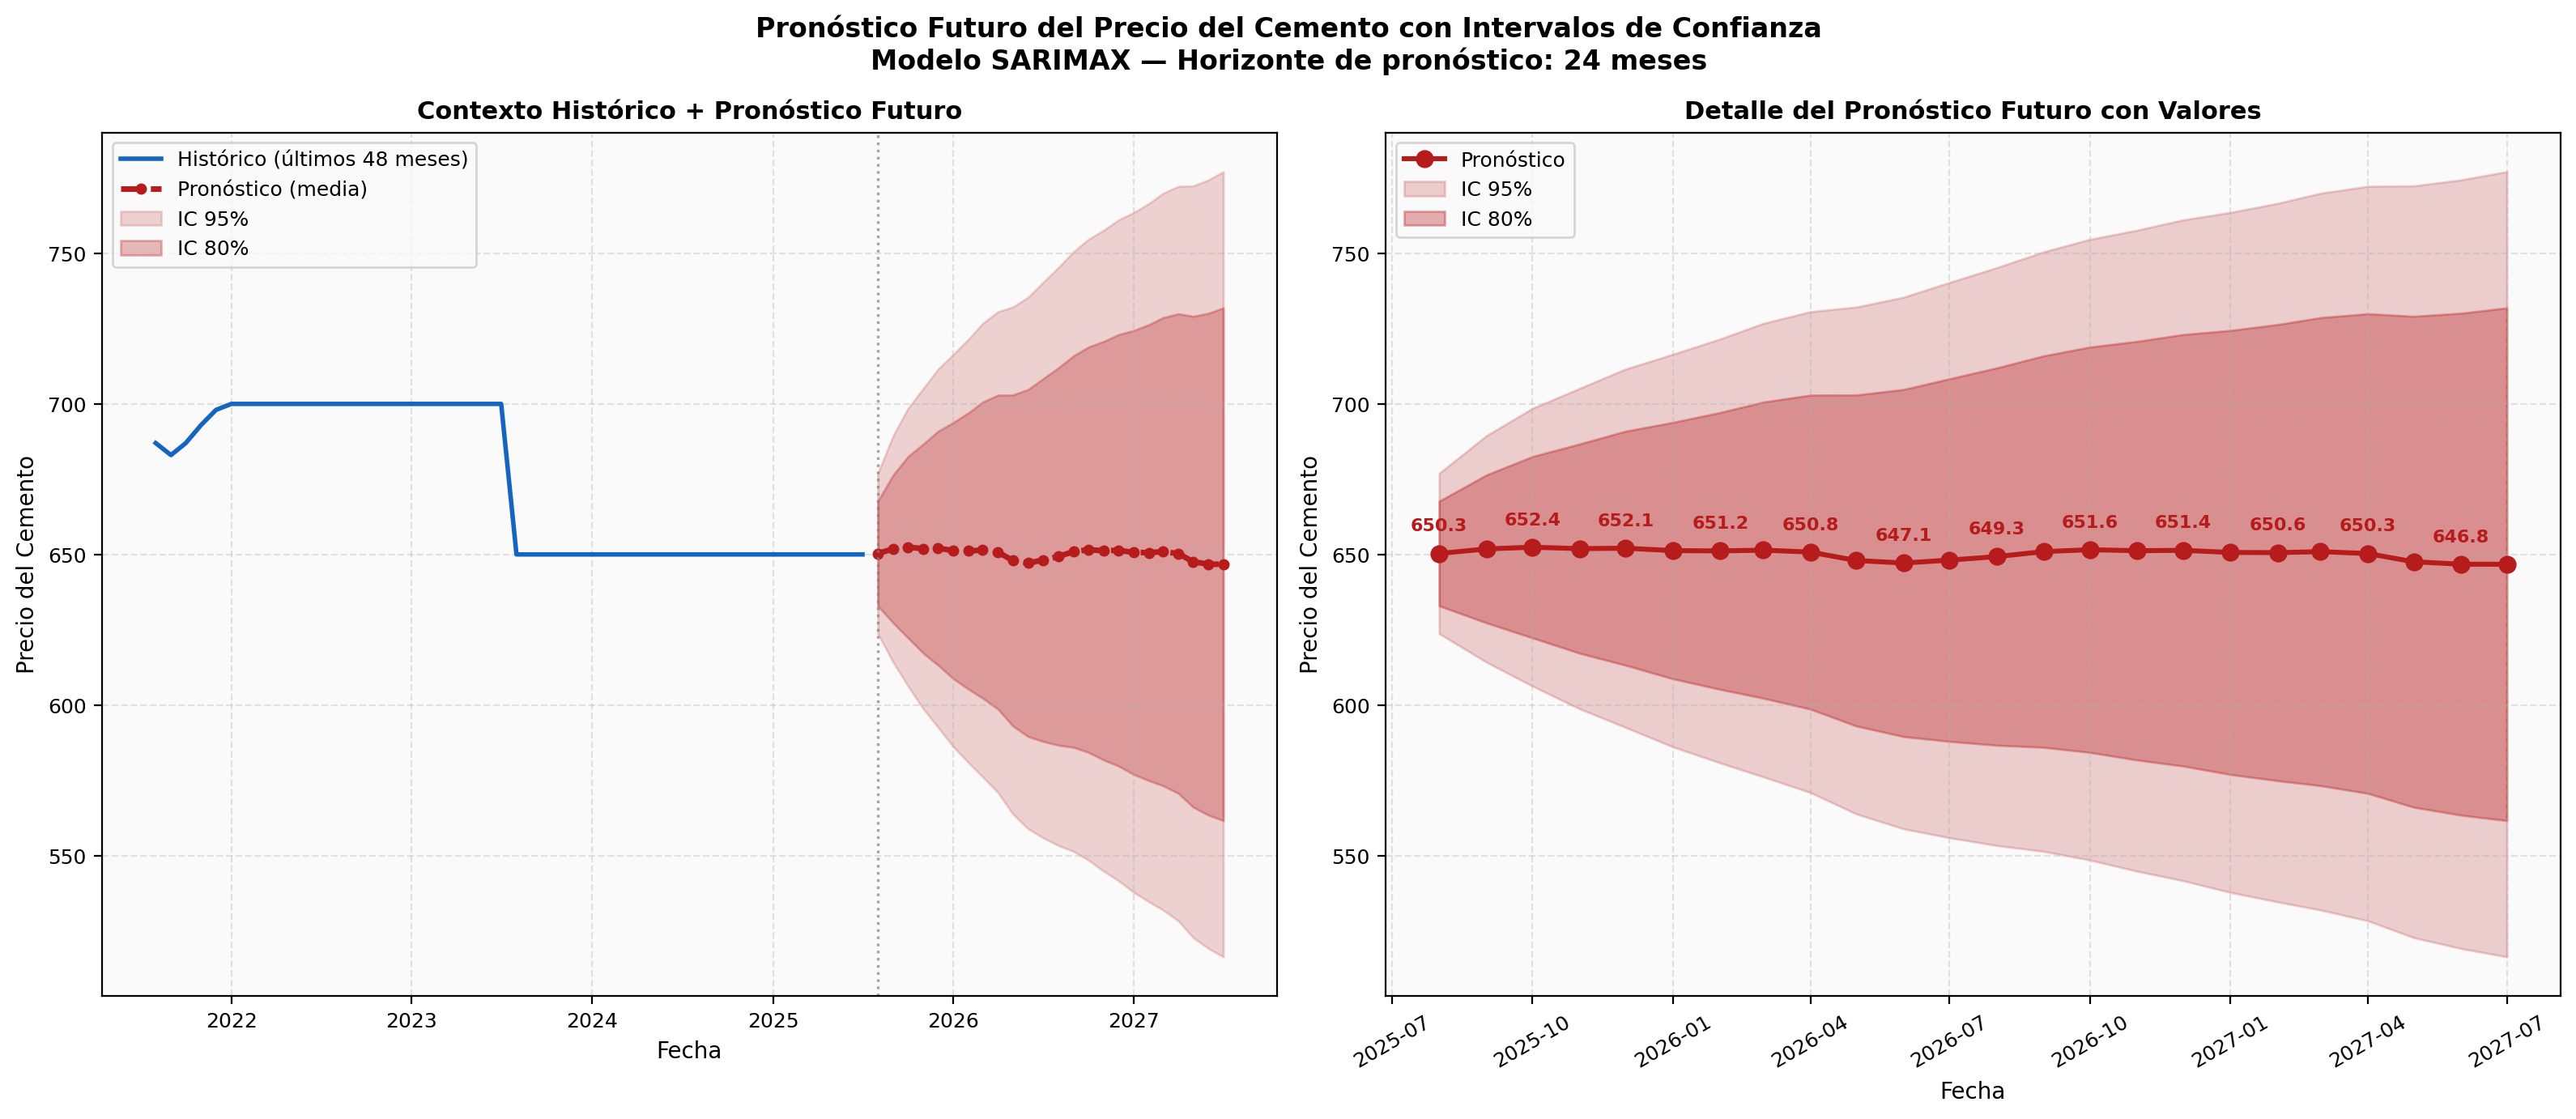
\includegraphics[width=\textwidth]{predicciones/prediccion_sarimax_ladrillo/graficos/09_pronostico_intervalo_confianza.png}
    \caption{Pronóstico del precio del ladrillo a 24 meses (agosto 2025 -- julio 2027) con intervalos de confianza al 95\,\%.}
    \label{fig:sarimax_ladrillo_pronostico_ic}
\end{figure}

\begin{figure}[ht]
    \centering
    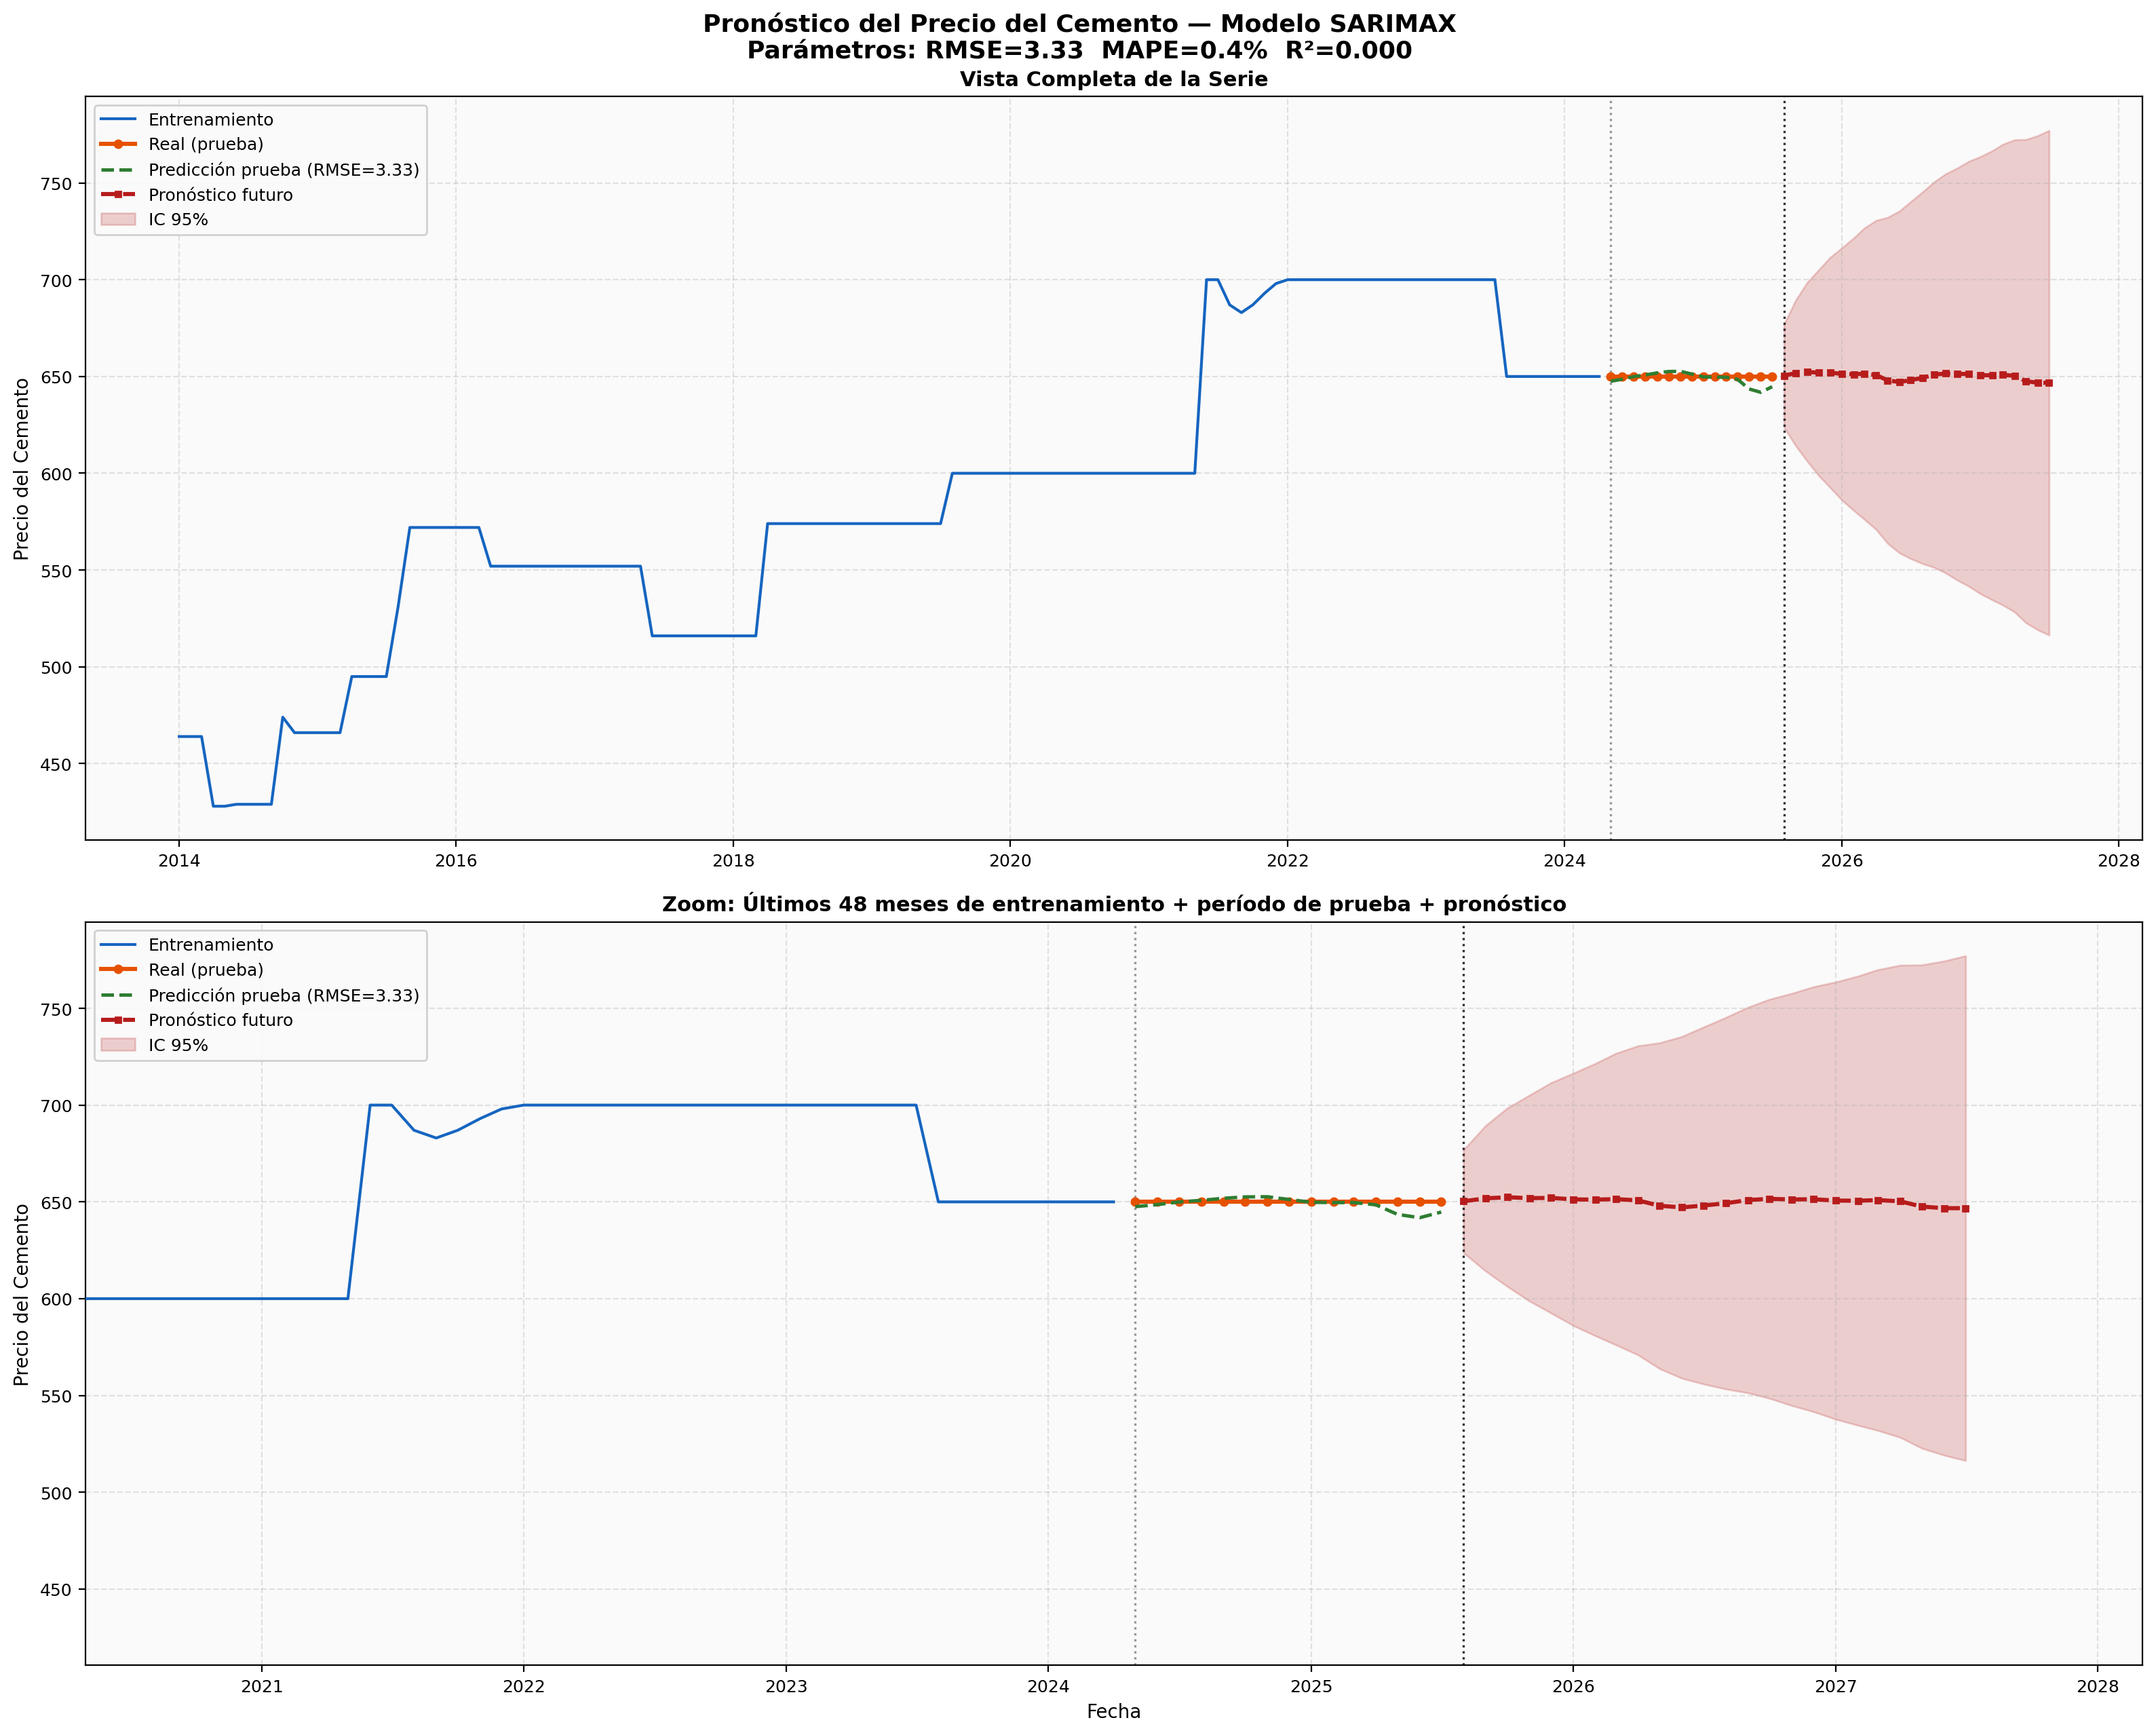
\includegraphics[width=\textwidth]{predicciones/prediccion_sarimax_ladrillo/graficos/06_pronostico_completo.png}
    \caption{Pronóstico completo del precio del ladrillo: serie histórica observada y proyección SARIMAX a 24 meses.}
    \label{fig:sarimax_ladrillo_pronostico_completo}
\end{figure}

\justify
Una vez validado el modelo, se generó el pronóstico del precio mensual del ladrillo para el horizonte de 24 meses comprendido entre agosto de 2025 y julio de 2027. Las Figuras \ref{fig:sarimax_ladrillo_pronostico_ic} y \ref{fig:sarimax_ladrillo_pronostico_completo} presentan el pronóstico puntual y el intervalo de confianza al 95\,\%, junto con la serie histórica completa.

\justify
El pronóstico puntual converge hacia un valor estable de aproximadamente Gs.~650, consistente con la naturaleza del modelo SARIMAX$(0,1,0)$. El intervalo de confianza al 95\,\% se amplía progresivamente con el horizonte de predicción: para agosto de 2025 el rango es de Gs.~[624 -- 677], mientras que para julio de 2027 se extiende a Gs.~[516 -- 777]. Este ensanchamiento, análogo al observado en el modelo del cemento, refleja la incertidumbre acumulada inherente a las proyecciones de largo plazo.

\justify
La Tabla \ref{tab:sarimax_ladrillo_pronostico} sintetiza los valores pronosticados para los primeros doce meses del horizonte de predicción.

\begin{table}[ht]
    \centering
    \caption{Pronóstico mensual del precio del ladrillo (Gs.) para el período agosto 2025 -- julio 2026, con intervalo de confianza al 95\,\%.}
    \label{tab:sarimax_ladrillo_pronostico}
    \begin{tabular}{lccc}
        \toprule
        \textbf{Mes} & \textbf{Pronóstico (Gs.)} & \textbf{IC Inferior} & \textbf{IC Superior} \\
        \midrule
        Agosto 2025      & 650 & 624 & 677 \\
        Septiembre 2025  & 652 & 614 & 689 \\
        Octubre 2025     & 652 & 606 & 698 \\
        Noviembre 2025   & 652 & 599 & 705 \\
        Diciembre 2025   & 652 & 593 & 712 \\
        Enero 2026       & 651 & 586 & 716 \\
        Febrero 2026     & 651 & 581 & 722 \\
        Marzo 2026       & 651 & 576 & 727 \\
        Abril 2026       & 651 & 571 & 731 \\
        Mayo 2026        & 648 & 564 & 732 \\
        Junio 2026       & 647 & 559 & 735 \\
        Julio 2026       & 648 & 556 & 740 \\
        \bottomrule
    \end{tabular}
\end{table}

\subsubsection{Modelo SARIMAX: Escenarios con y sin Efecto Pandémico}

\justify
Al igual que para el cemento, se generaron dos proyecciones paralelas para el precio del ladrillo bajo escenarios alternativos de pandemia. Las Figuras \ref{fig:sarimax_ladrillo_sin_covid} y \ref{fig:sarimax_ladrillo_con_covid} presentan los pronósticos resultantes.

\begin{figure}[ht]
    \centering
    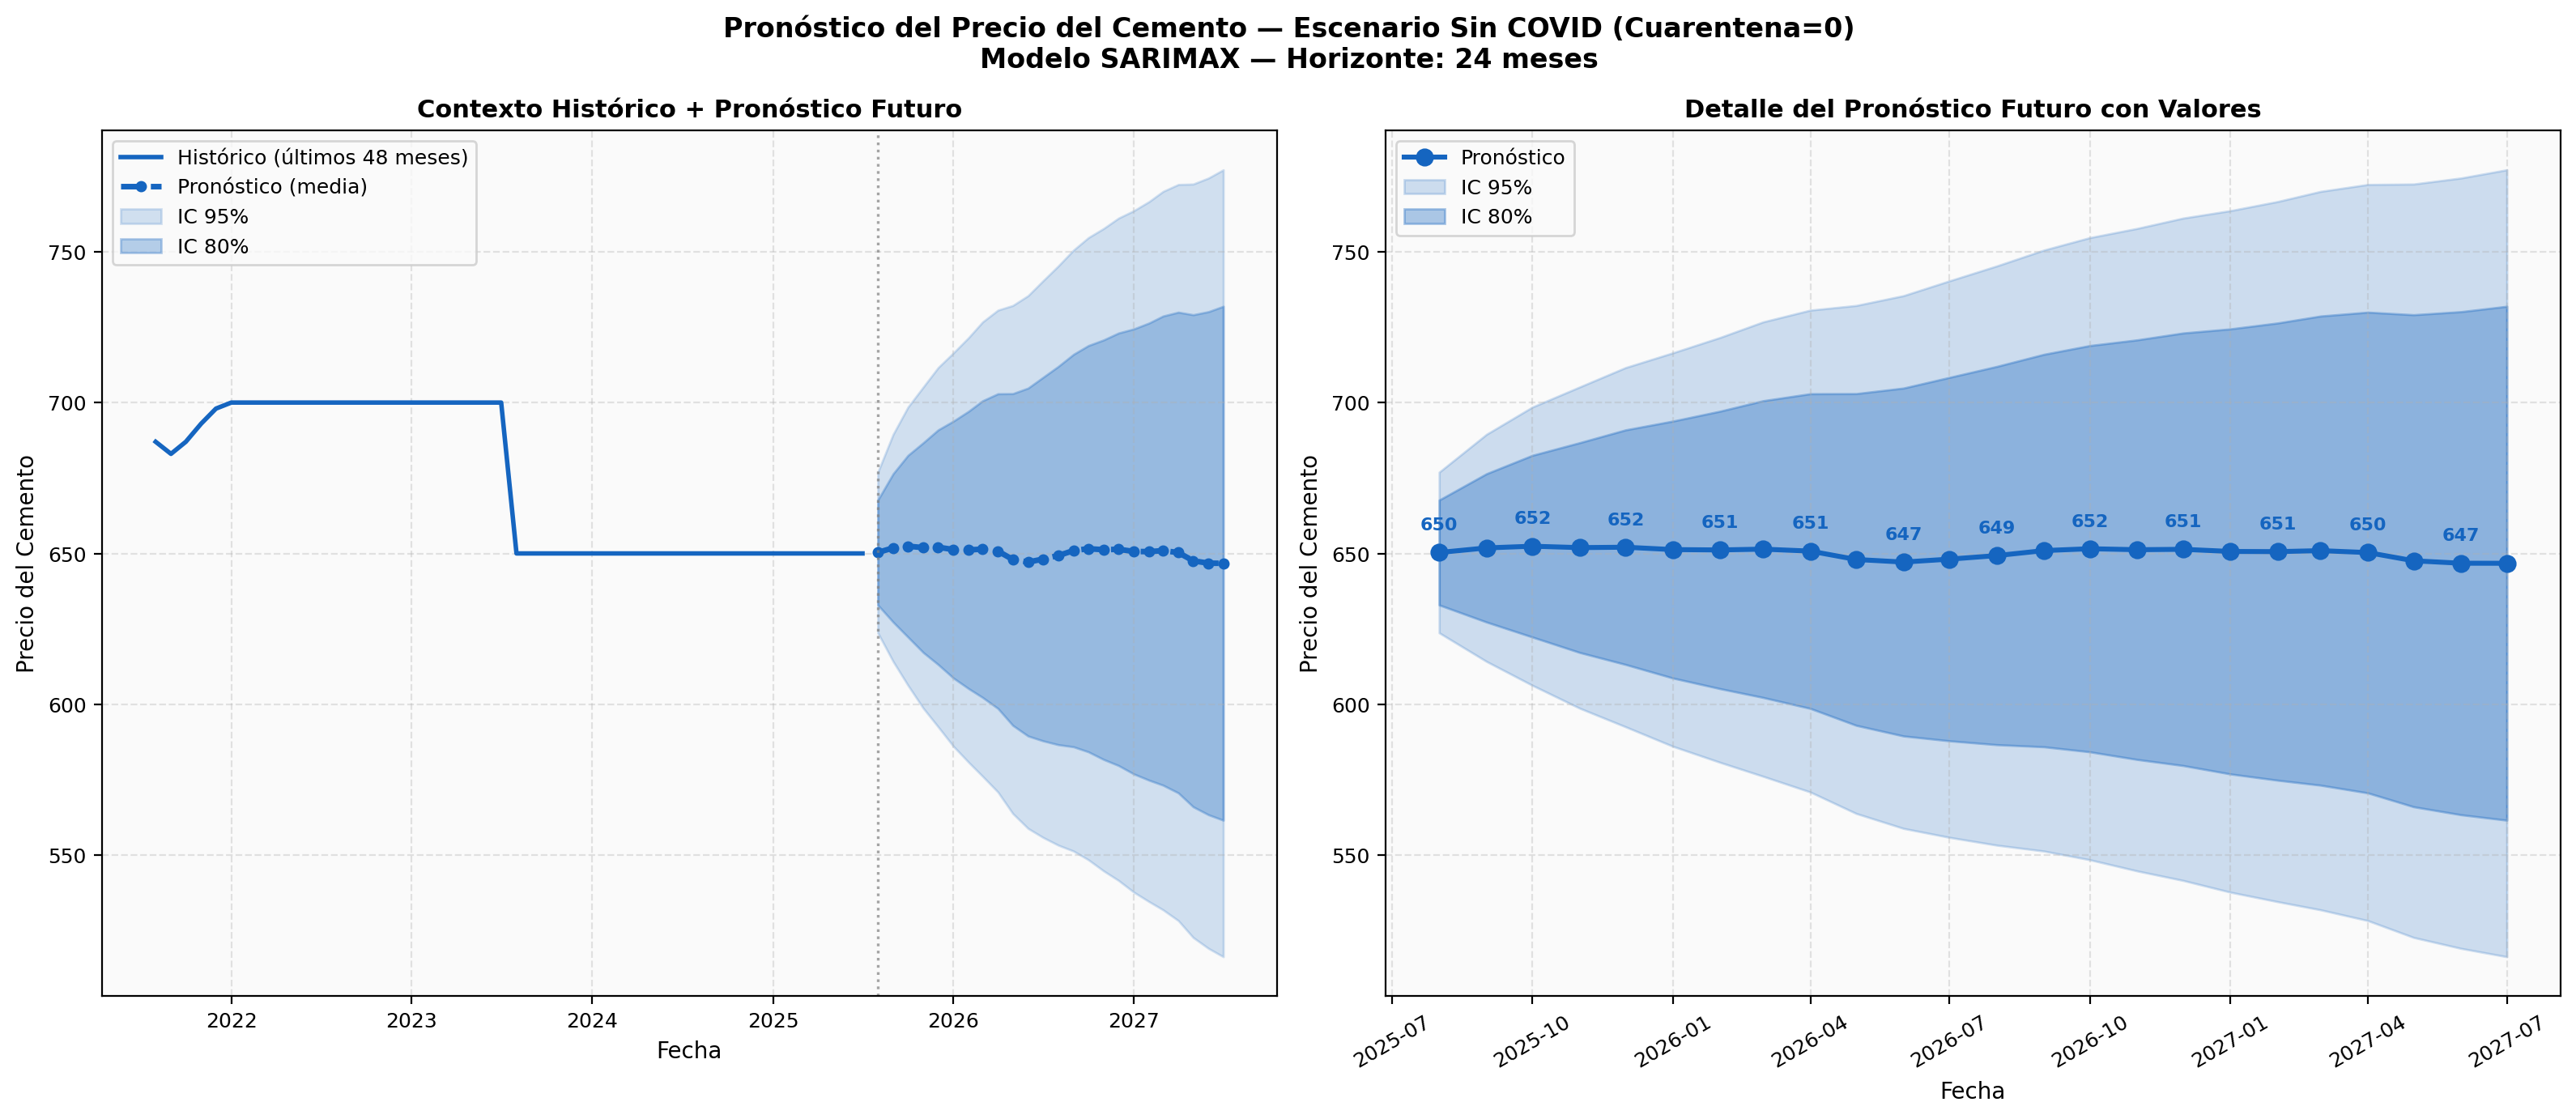
\includegraphics[width=\textwidth]{predicciones/prediccion_sarimax_ladrillo/graficos/12a_pronostico_sin_covid.png}
    \caption{Pronóstico SARIMAX del precio del ladrillo a 24 meses -- escenario sin efecto pandémico.}
    \label{fig:sarimax_ladrillo_sin_covid}
\end{figure}

\begin{figure}[ht]
    \centering
    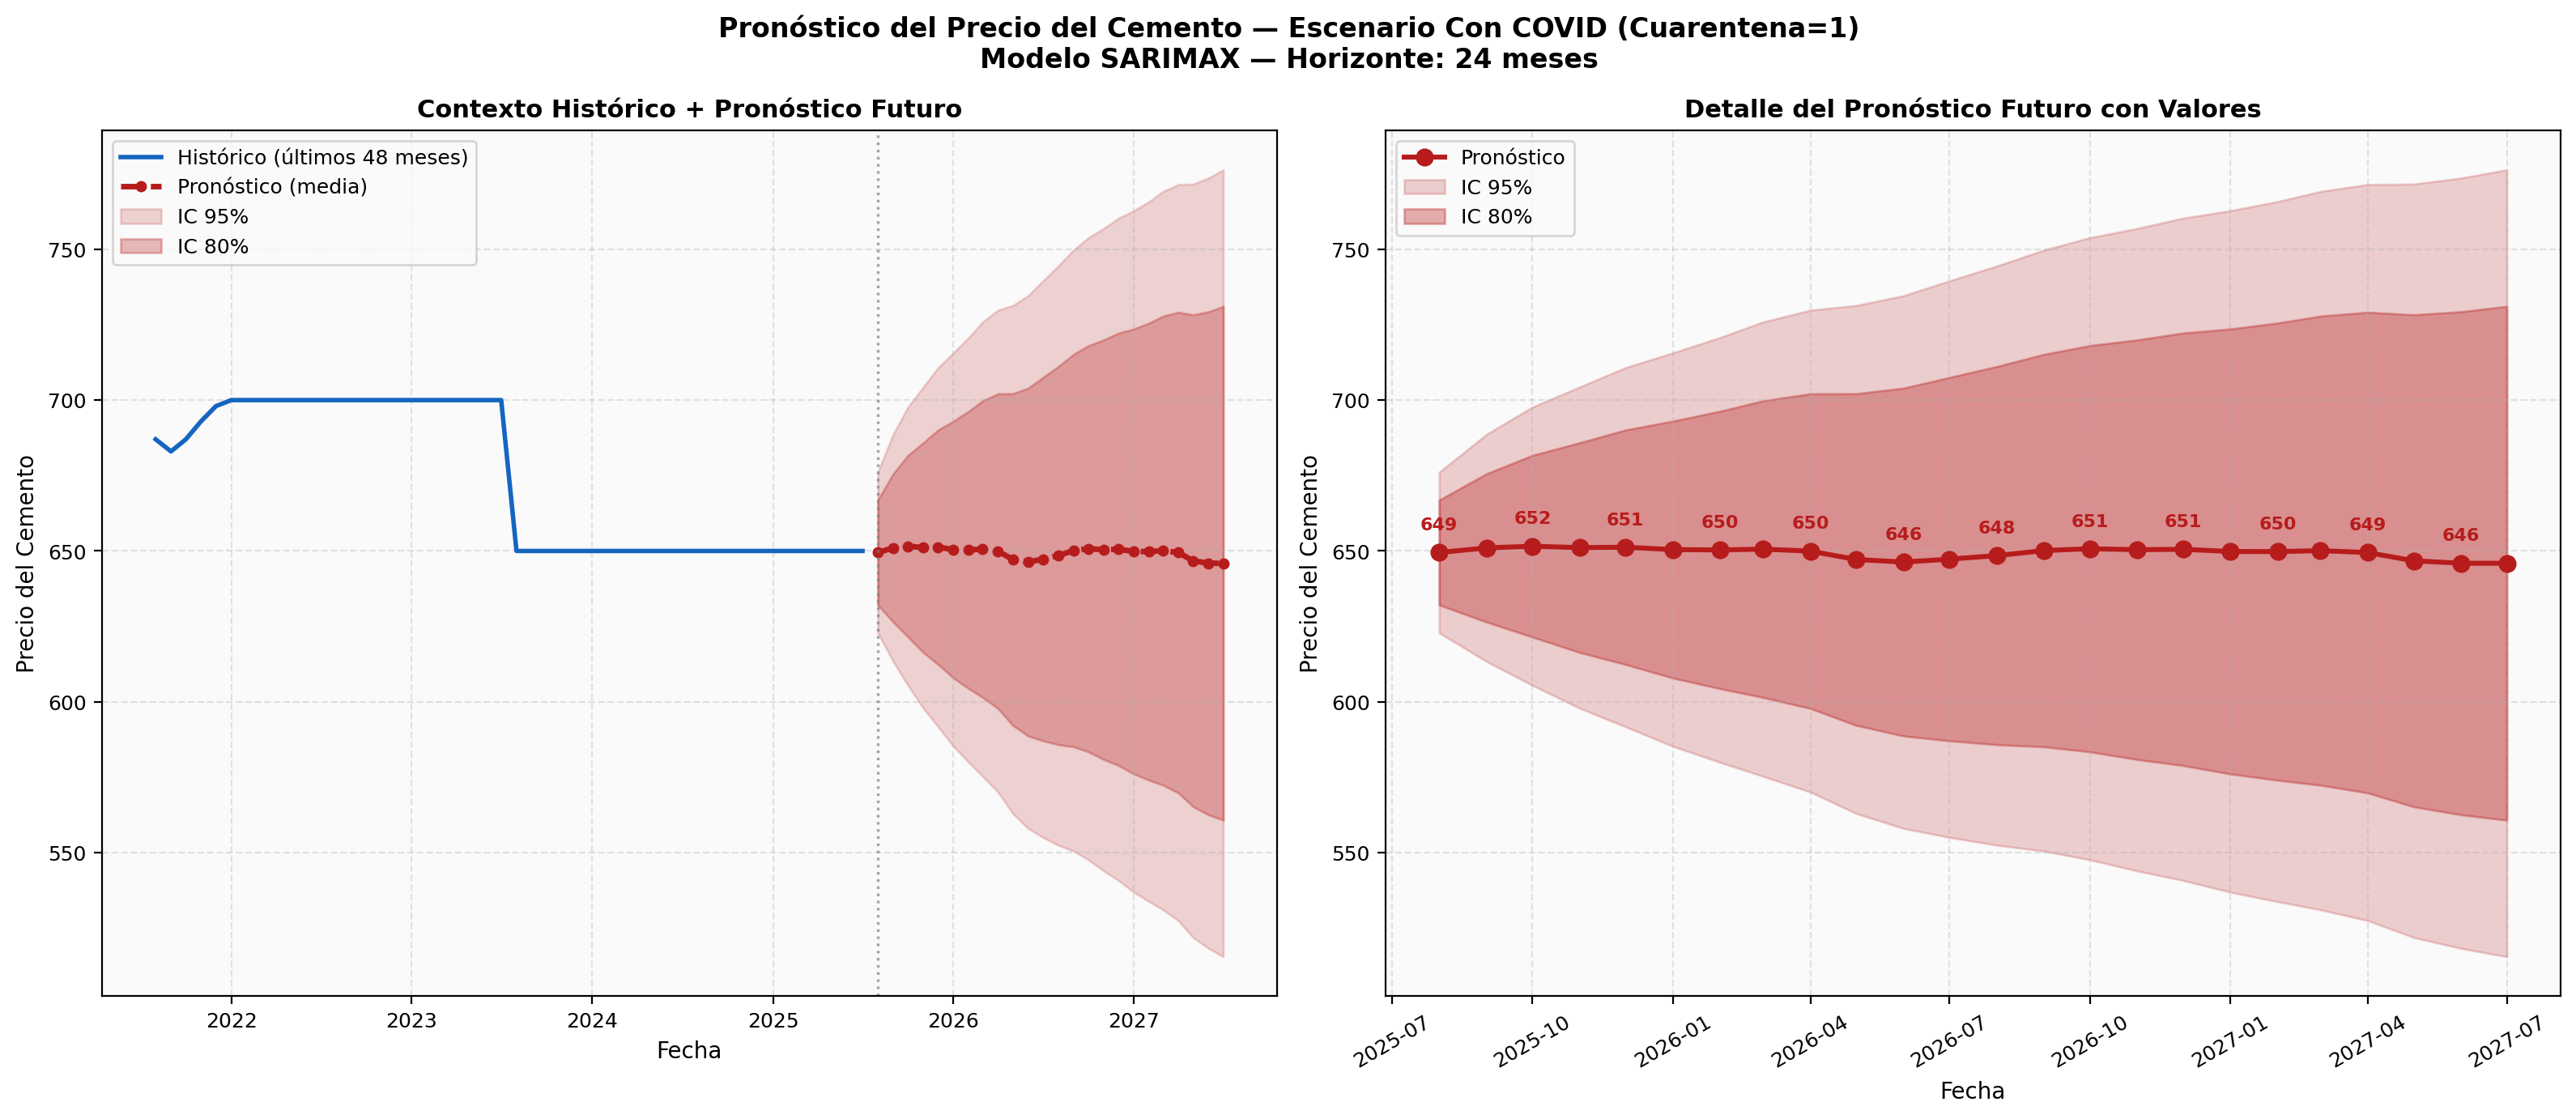
\includegraphics[width=\textwidth]{predicciones/prediccion_sarimax_ladrillo/graficos/12b_pronostico_con_covid.png}
    \caption{Pronóstico SARIMAX del precio del ladrillo a 24 meses -- escenario con efecto pandémico.}
    \label{fig:sarimax_ladrillo_con_covid}
\end{figure}

\justify
La diferencia entre ambos escenarios es de apenas Gs.~$-0{,}82$ por mes, un valor aún más reducido que el observado para el cemento (Gs.~$-23{,}48$) y completamente insignificante frente al nivel de precios de la serie (Gs.~650). Este resultado es coherente con el coeficiente estimado para la variable \texttt{Cuarentena} en el modelo SARIMAX del ladrillo ($-0{,}819$~Gs., $p=0{,}999$), que resultó estadísticamente no significativo. La insensibilidad del modelo SARIMAX ante el \textit{shock} pandémico se repite en ambos materiales de construcción, confirmando que la estructura lineal integrada del modelo ---capaz de capturar la tendencia general y la contribución hidrológica--- carece de la flexibilidad necesaria para representar los efectos no lineales y asimétricos de perturbaciones como la pandemia de COVID-19. Los modelos LSTM y GRU que se presentan en las secciones siguientes ofrecen un contraste instructivo al respecto.

% resultados_lstm.tex  --  Sección 4.3
% Predicción LSTM para Cemento y Ladrillo Común

\section{Predicción de los Precios del Cemento y del Ladrillo Común con Long Short-Term Memory (LSTM)}

\vspace{0.3cm}
\justify
En esta sección se presentan los resultados de aplicar una red LSTM (\textit{Long Short-Term Memory}) a la predicción de los precios mensuales del cemento y del ladrillo común. Para cada material se entrenaron dos modelos independientes: uno para el escenario sin efecto pandémico y otro para el escenario con efecto pandémico. Ambos fueron implementados con TensorFlow 2.19.0 / Keras, y sus hiperparámetros fueron optimizados de forma independiente con Optuna. La partición temporal es idéntica en todos los casos: 95 meses de entrenamiento, 20 meses de validación y 22 meses de prueba. Las variables de entrada son 7: precio promedio polinomial de grado 2, nivel del río Paraguay, indicador de cuarentena COVID-19, rezago de un mes, media móvil de 3 meses, y las componentes sinusoidal y cosenoidal del mes. Los intervalos de confianza al 95\,\% se estimaron mediante Monte Carlo Dropout ($N=100$ simulaciones).

% ============================================================
%  CEMENTO
% ============================================================
\subsection{Predicción del Precio del Cemento}

\justify
Para el cemento, la búsqueda de hiperparámetros con Optuna convergió a la misma configuración en ambos escenarios (sin y con efecto pandémico), lo que indica que la arquitectura óptima para esta serie es robusta a la inclusión o exclusión de la variable pandémica en el entrenamiento. Las métricas de evaluación sobre el conjunto de prueba son asimismo idénticas entre escenarios (RMSE de prueba: Gs.~1.619,75). Por esta razón, la descripción del modelo, la evaluación y el análisis de residuos se presentan una sola vez; los resultados se diferencian únicamente en el pronóstico a 24 meses.

\subsubsection{Análisis Exploratorio de la Serie}

\begin{figure}[htbp]
    \centering
    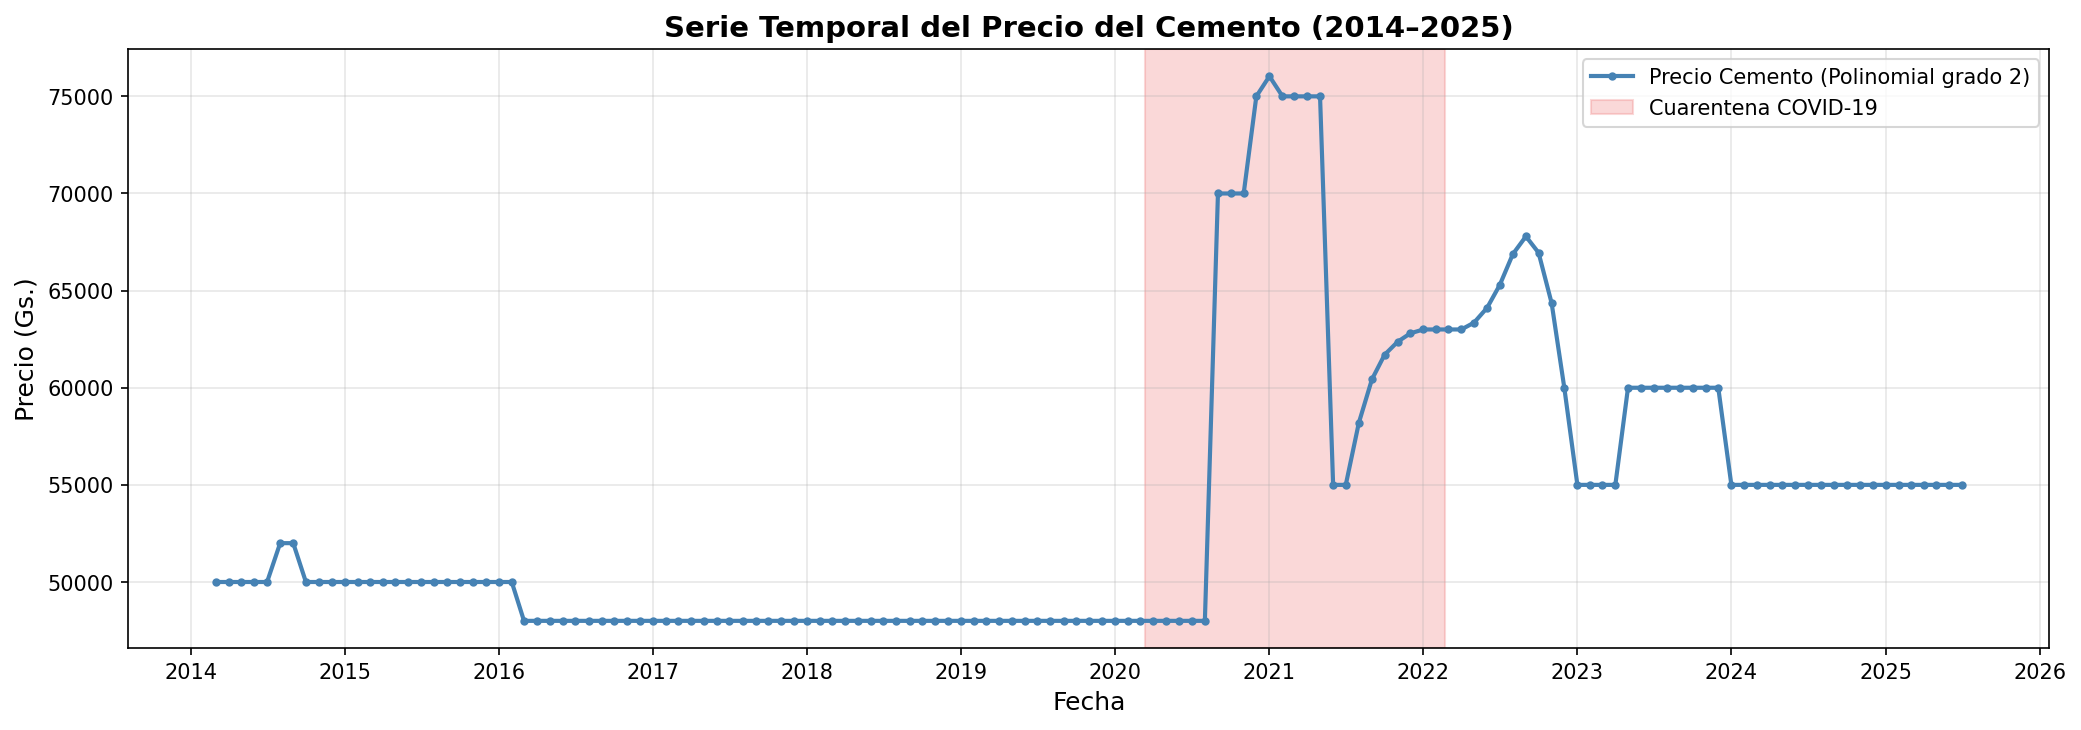
\includegraphics[width=\textwidth]{predicciones/prediccion_cemento_lstm/resultados_sin_covid/eda_01_serie_precios_cemento.png}
    \caption{Serie histórica mensual del precio del cemento (Gs.), período 2014--2025.}
    \label{fig:lstm_cemento_eda_serie}
\end{figure}

\begin{figure}[htbp]
    \centering
    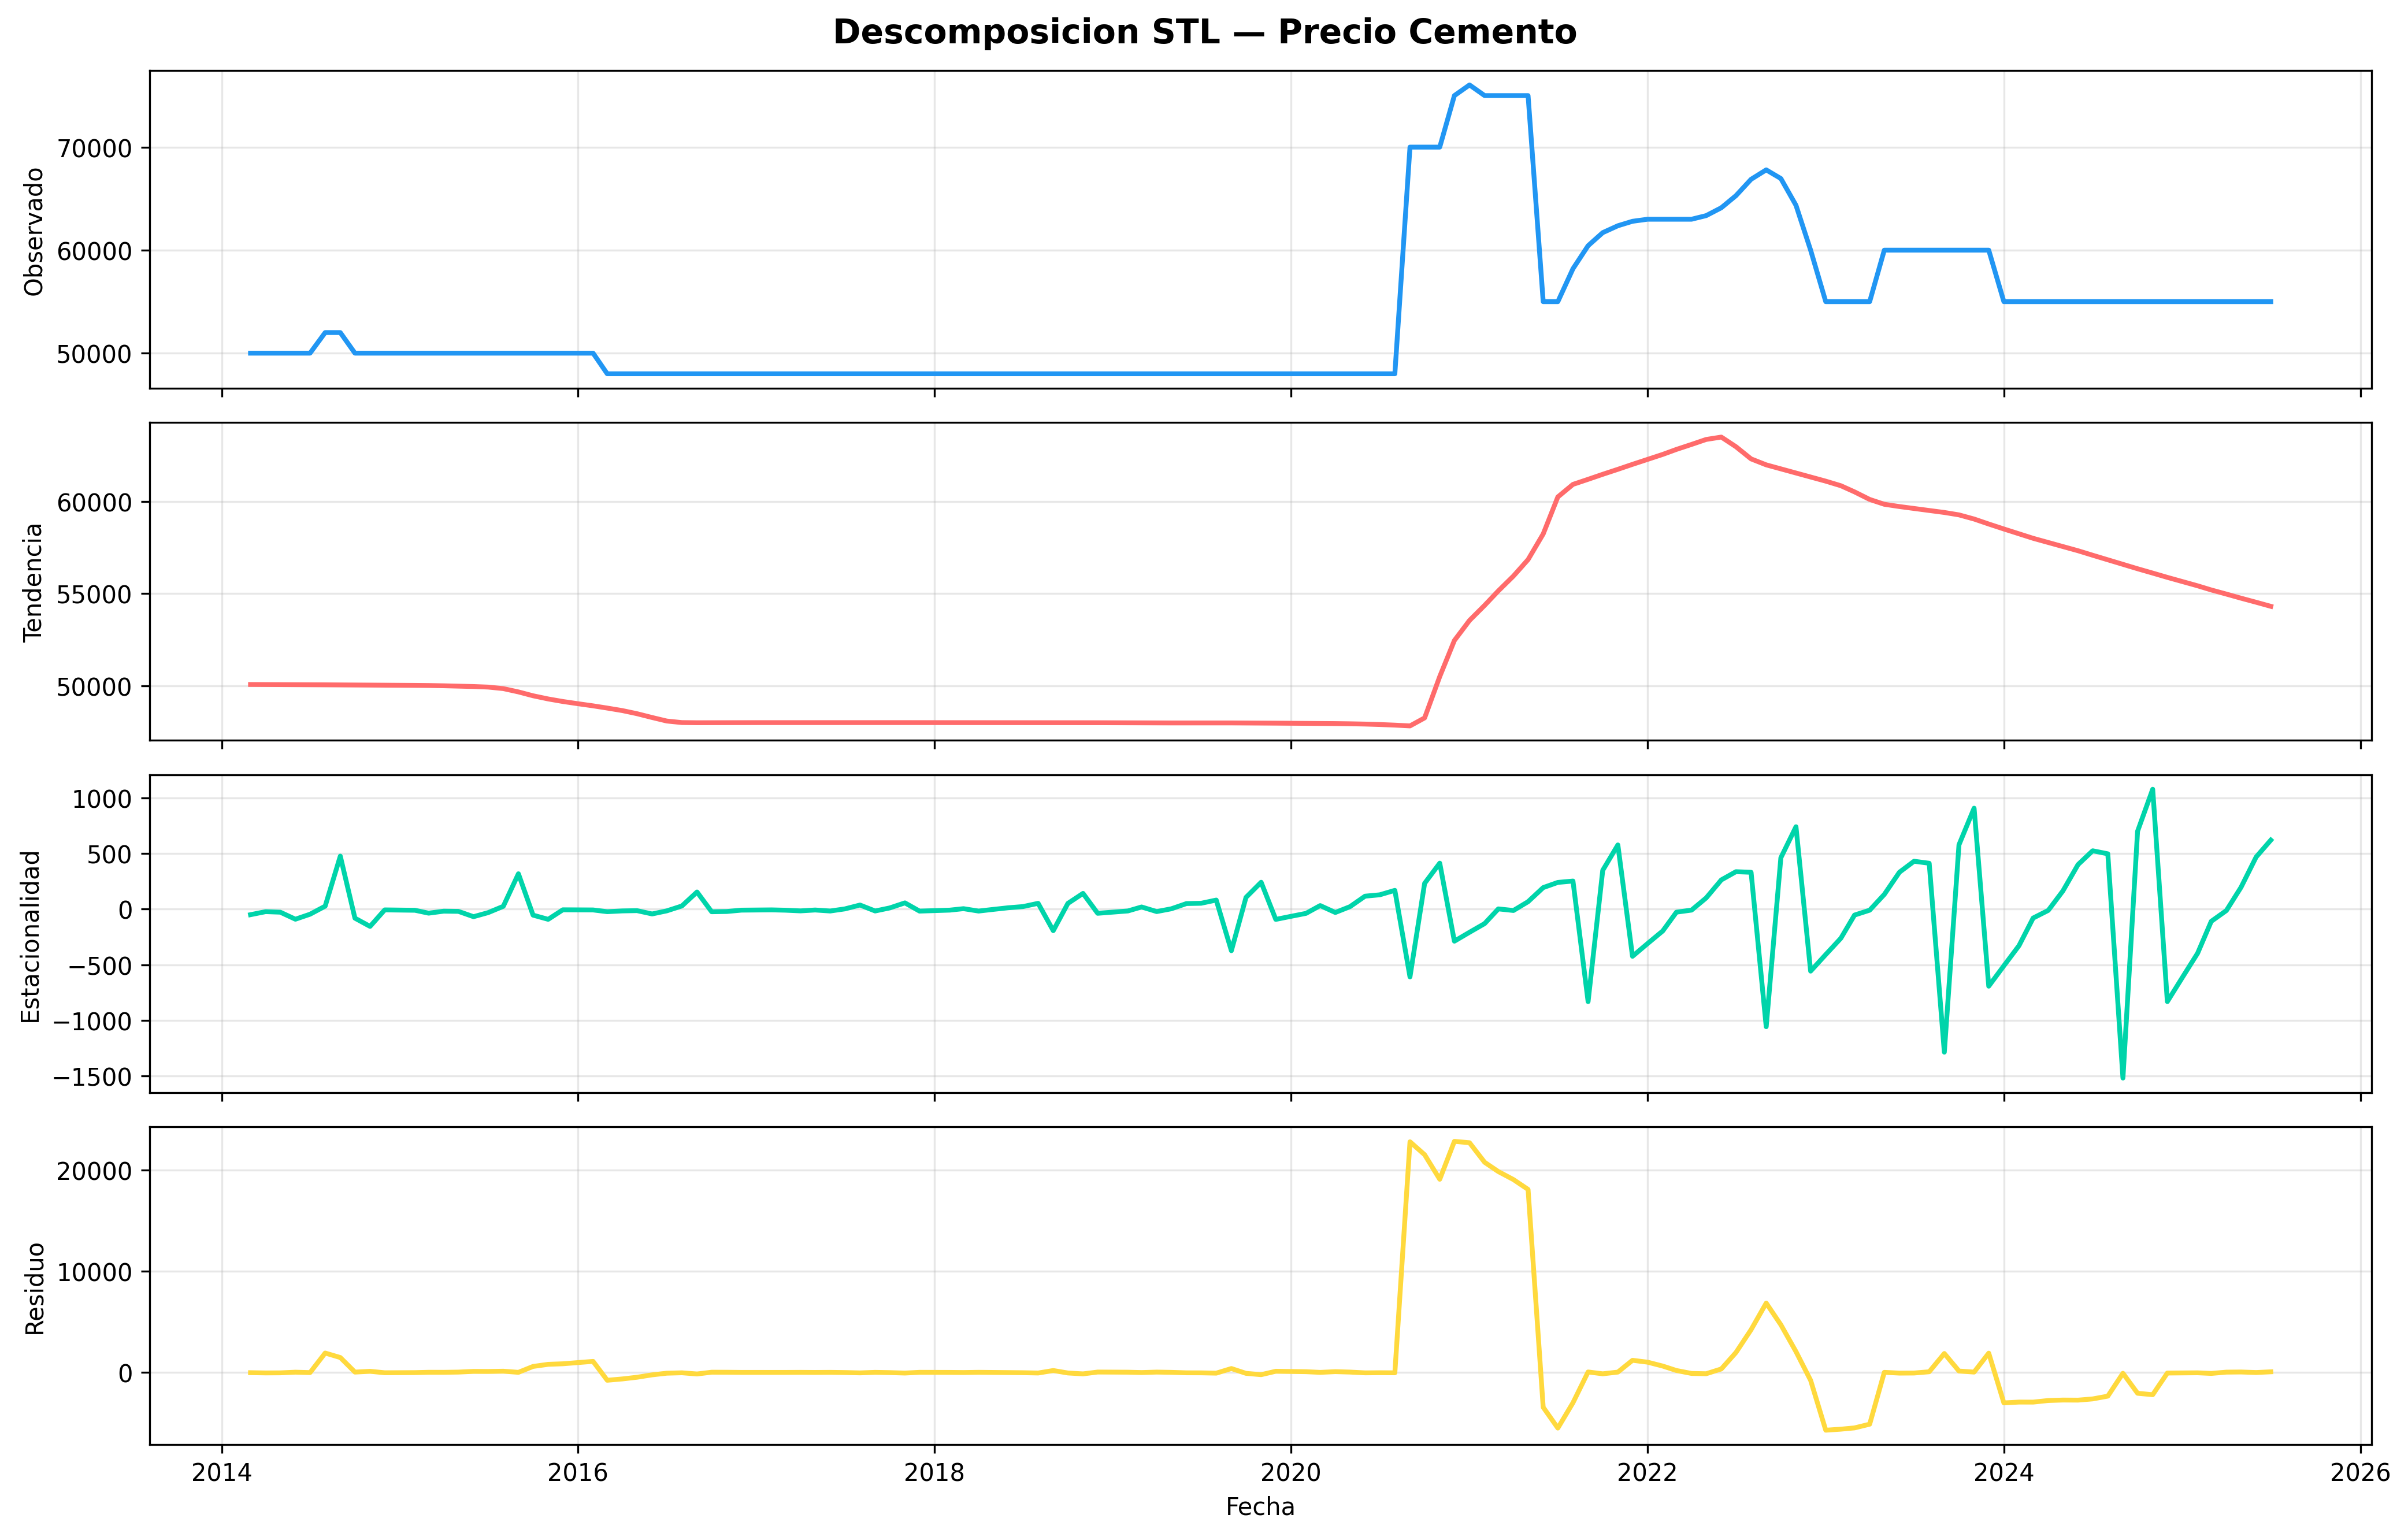
\includegraphics[width=\textwidth]{predicciones/prediccion_cemento_lstm/resultados_sin_covid/eda_stl_decomposition.png}
    \caption{Descomposición STL de la serie del precio del cemento: tendencia, estacionalidad y residuo.}
    \label{fig:lstm_cemento_eda_stl}
\end{figure}

\begin{figure}[htbp]
    \centering
    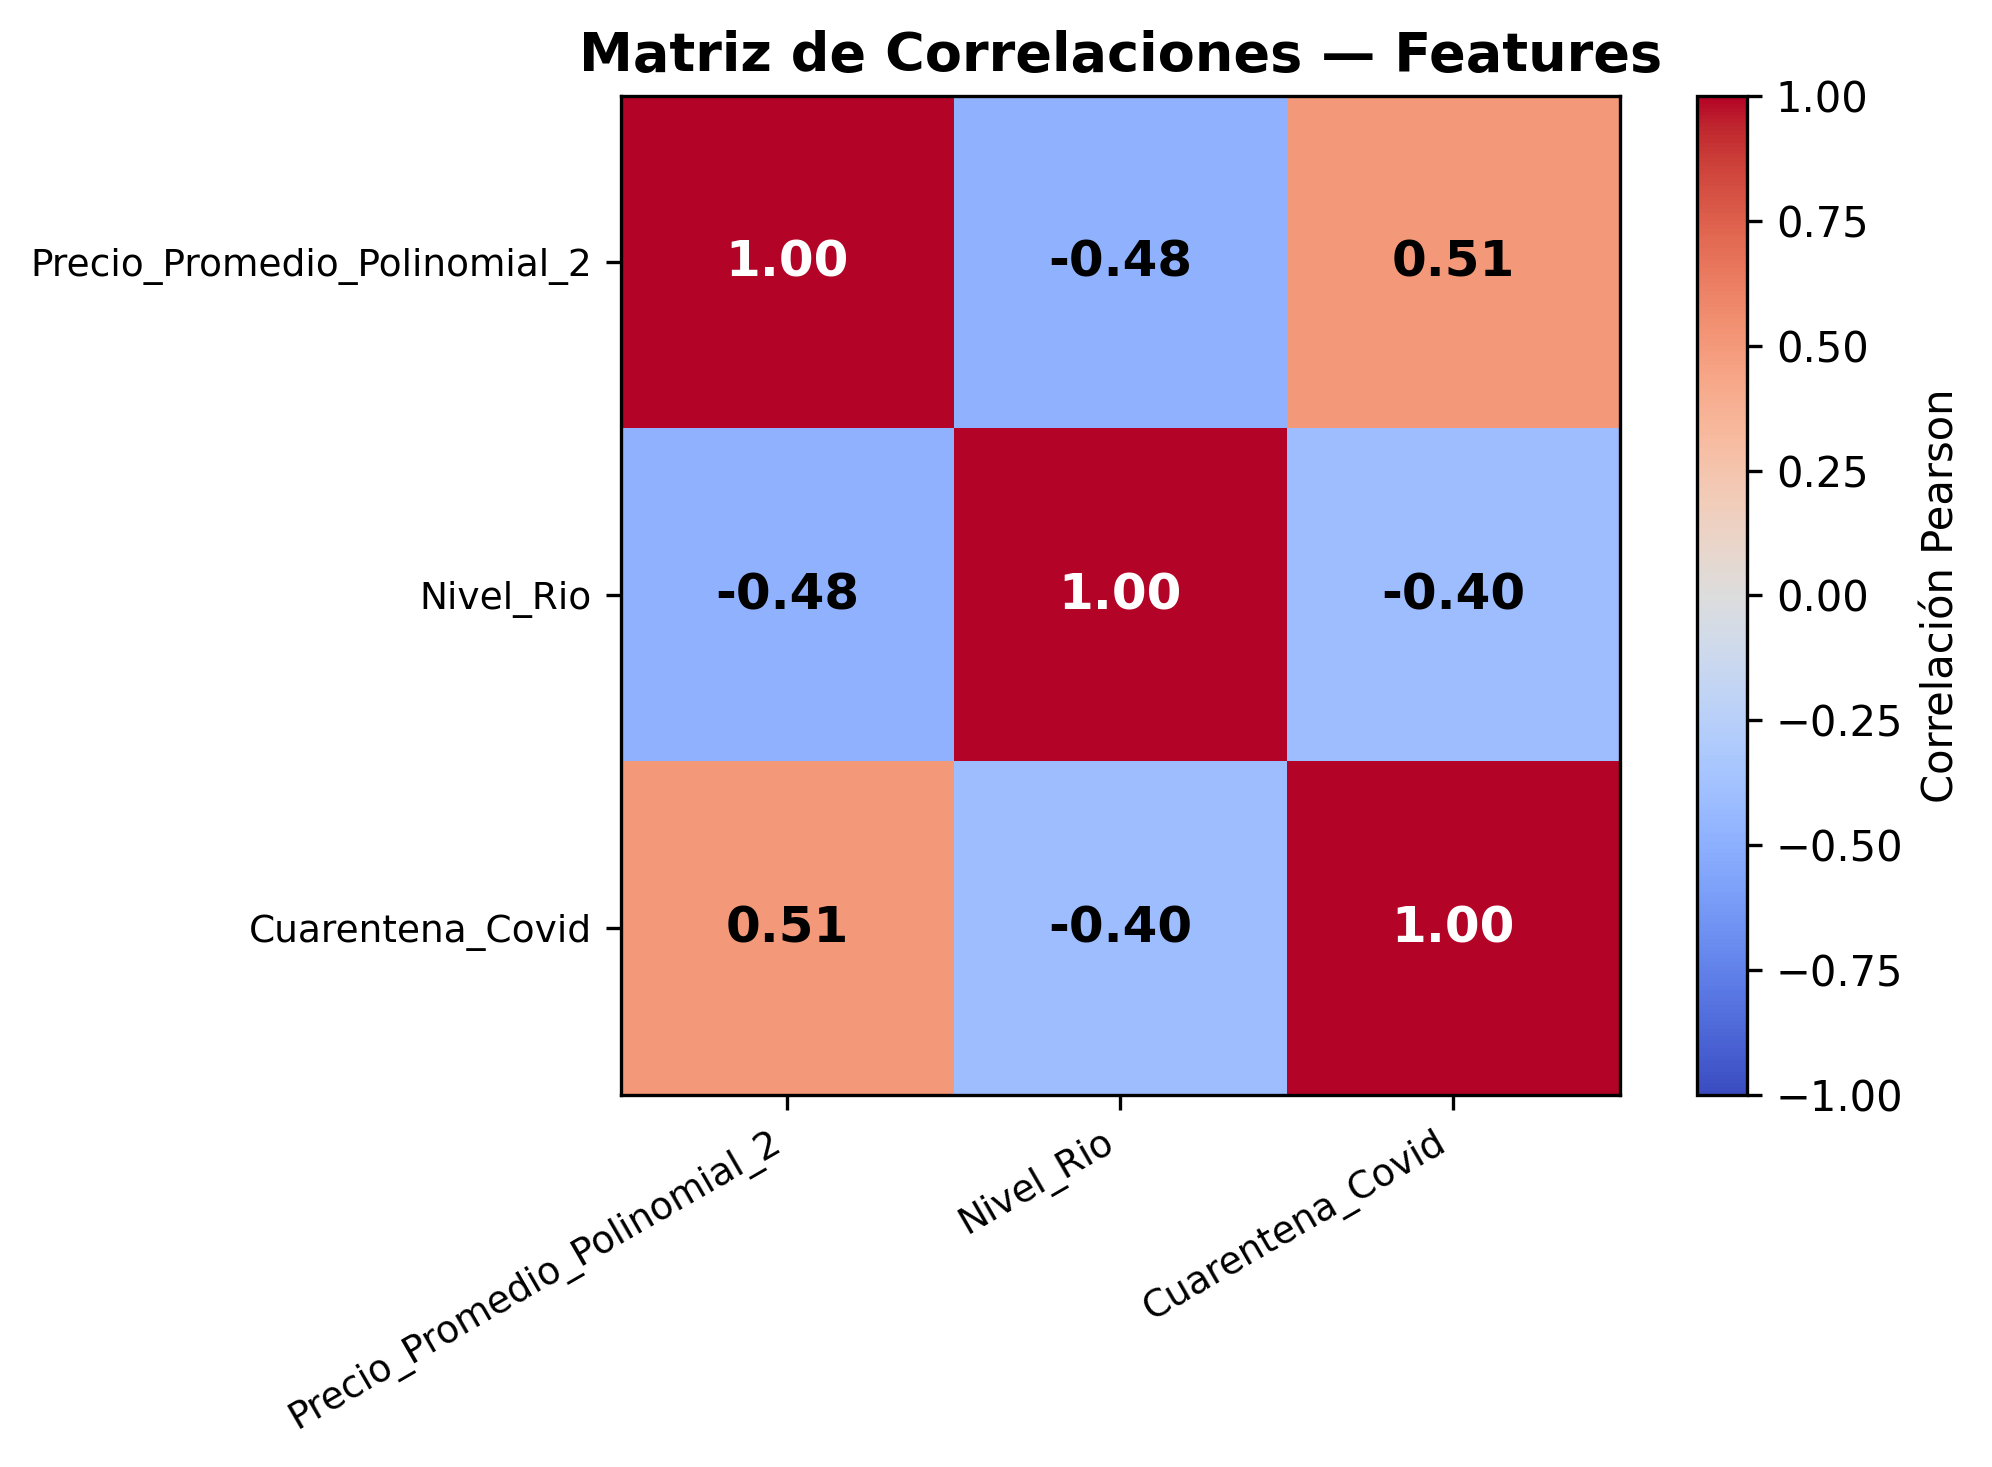
\includegraphics[width=\textwidth]{predicciones/prediccion_cemento_lstm/resultados_sin_covid/eda_correlaciones_heatmap.png}
    \caption{Mapa de calor de correlaciones entre las variables de entrada del modelo LSTM para cemento.}
    \label{fig:lstm_cemento_eda_corr}
\end{figure}

\subsubsection{Hiperparámetros y Arquitectura}

\justify
La búsqueda automática de hiperparámetros con Optuna seleccionó una arquitectura de una sola capa LSTM con 64 unidades ocultas, sin bidireccionalidad ni \textit{dropout}. El optimizador elegido fue Adam con tasa de aprendizaje $\text{lr}=0{,}001$ y regularización de pesos $\lambda=10^{-5}$. El \textit{lookback} quedó fijado en 6 meses y el \textit{batch size} en 4. No se aplicó ningún \textit{scheduler} de tasa de aprendizaje. La Tabla~\ref{tab:lstm_cemento_hiper} resume estos parámetros.

\begin{table}[htbp]
\centering
\caption{Hiperparámetros óptimos del modelo LSTM para cemento, seleccionados por Optuna.}
\label{tab:lstm_cemento_hiper}
\begin{tabular}{ll}
\toprule
\textbf{Hiperparámetro} & \textbf{Valor} \\
\midrule
Capas LSTM          & 1 \\
Unidades ocultas    & 64 \\
Bidireccional       & No \\
Dropout             & 0,0 \\
Dropout recurrente  & 0,0 \\
Optimizador         & Adam \\
Tasa de aprendizaje & 0,001 \\
Regularización L2   & $10^{-5}$ \\
Lookback            & 6 meses \\
Batch size          & 4 \\
Scheduler           & Ninguno \\
Parámetros entrenables & 18.497 \\
\bottomrule
\end{tabular}
\end{table}

\subsubsection{Curva de Aprendizaje}

\justify
El modelo final se entrenó durante 65 épocas sobre el conjunto de entrenamiento con \textit{early stopping} basado en el RMSE de validación. La Figura~\ref{fig:lstm_cemento_curva} muestra la evolución del error en ambas particiones.

\begin{figure}[htbp]
    \centering
    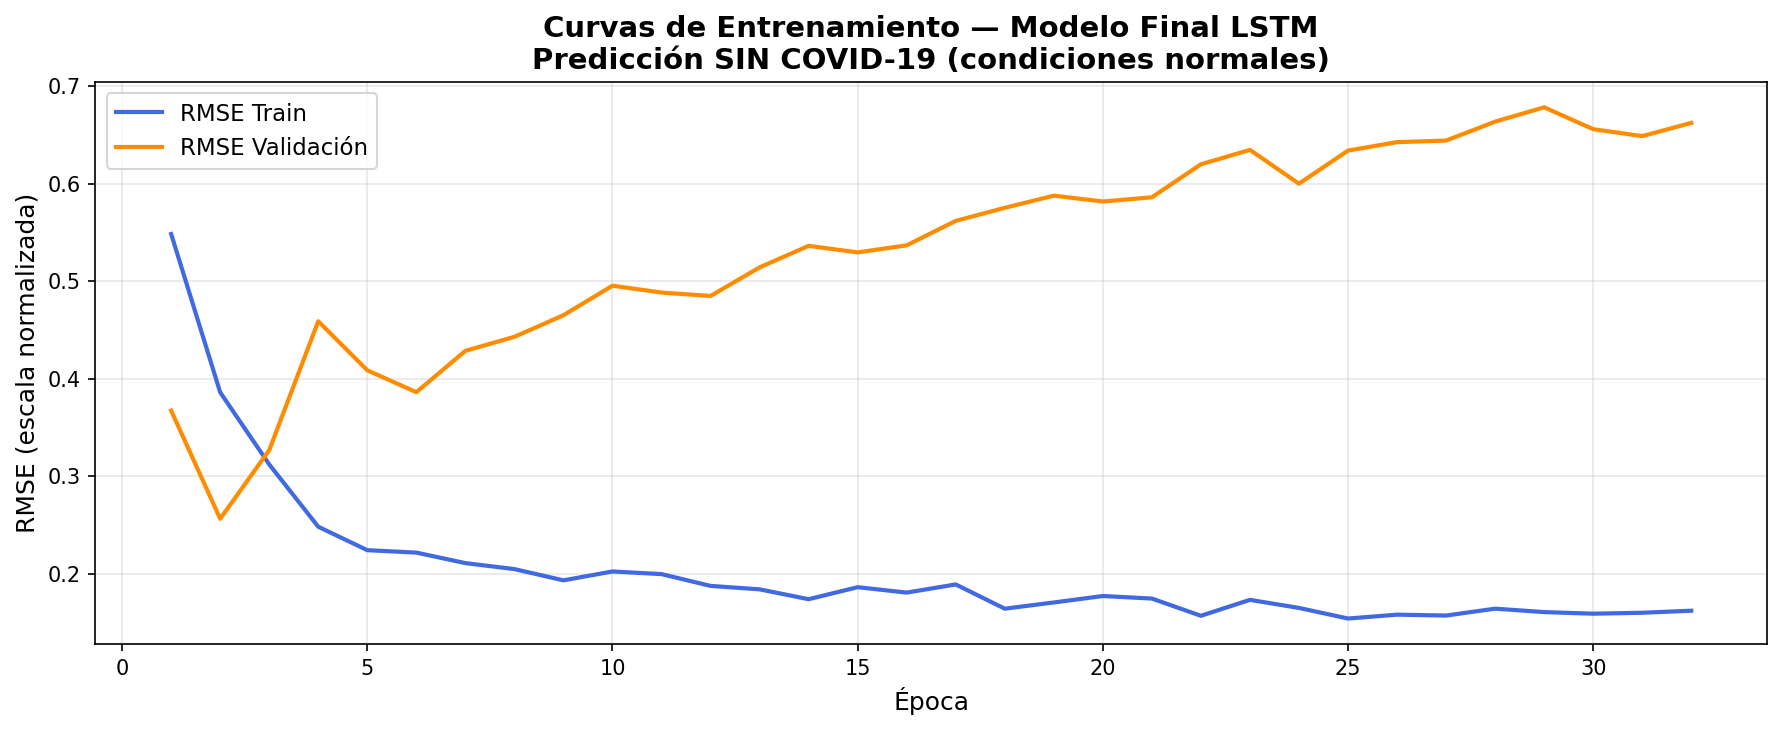
\includegraphics[width=0.85\textwidth]{predicciones/prediccion_cemento_lstm/resultados_sin_covid/final_01_curvas_entrenamiento.png}
    \caption{Curva de aprendizaje del modelo LSTM para cemento: RMSE de entrenamiento y validación por época.}
    \label{fig:lstm_cemento_curva}
\end{figure}

\justify
Se observa que el error de entrenamiento desciende rápidamente durante las primeras épocas y se estabiliza, mientras que el error de validación converge hacia un nivel ligeramente superior sin divergir de manera sostenida. Este comportamiento indica que el modelo generaliza correctamente sin presentar sobreajuste severo.

\subsubsection{Métricas de Evaluación}

\justify
La Tabla~\ref{tab:lstm_cemento_metricas} presenta el RMSE obtenido en los tres subconjuntos de datos, expresado en Guaraníes (Gs.).

\begin{table}[htbp]
\centering
\caption{Desempeño del modelo LSTM para cemento: RMSE en entrenamiento, validación y prueba.}
\label{tab:lstm_cemento_metricas}
\begin{tabular}{lrrr}
\toprule
\textbf{Métrica} & \textbf{Train} & \textbf{Val} & \textbf{Test} \\
\midrule
RMSE (Gs.) & 1.828,74 & 4.261,22 & 1.619,75 \\
\bottomrule
\end{tabular}
\end{table}

\justify
El RMSE de prueba de 1.619,75~Gs.\ resulta inferior al de entrenamiento (1.828,74~Gs.), lo que indica que el modelo no ha memorizado los datos de entrenamiento. El error de validación más elevado (4.261,22~Gs.) refleja que ese subconjunto contiene meses con mayor volatilidad de precios. En términos relativos, considerando que el precio del cemento oscila históricamente en el rango de Gs.~48.000 a Gs.~76.036, el RMSE de prueba representa un error relativo inferior al 4\%, resultado aceptable para una predicción mensual a nivel de mercado.

\subsubsection{Evaluación sobre el Conjunto de Prueba}

\begin{figure}[htbp]
    \centering
    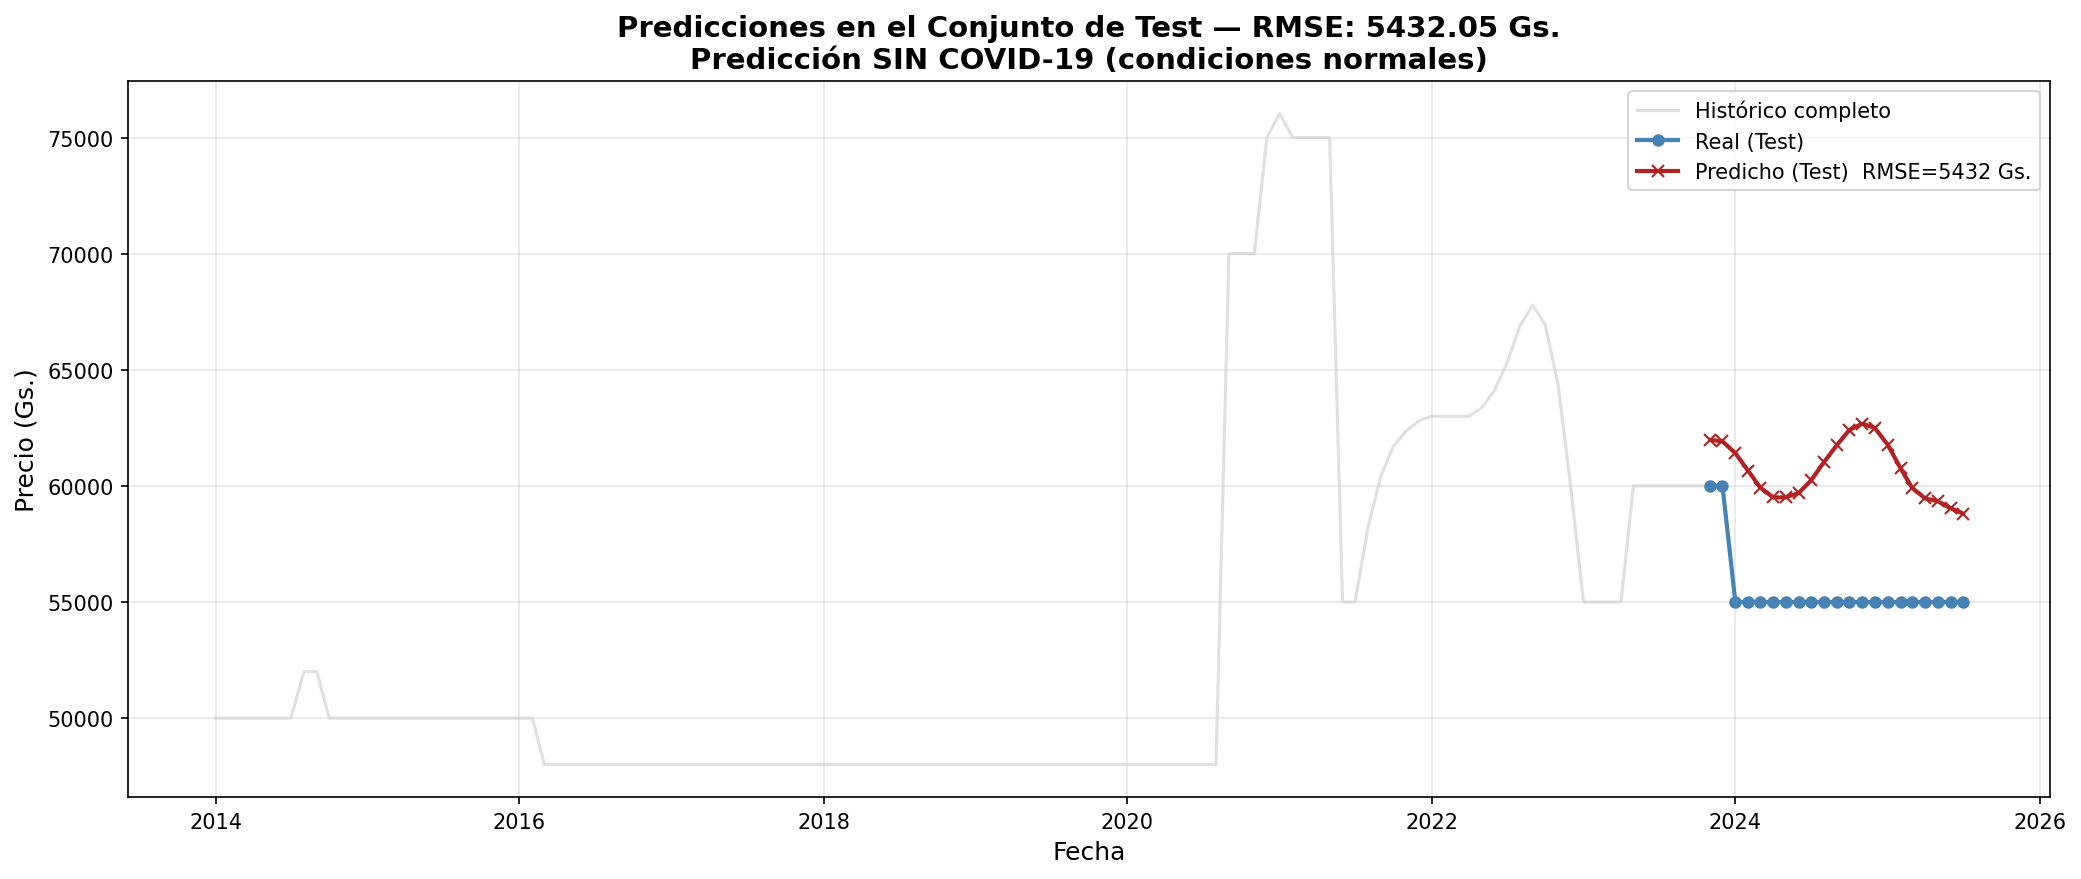
\includegraphics[width=\textwidth]{predicciones/prediccion_cemento_lstm/resultados_sin_covid/final_02_prediccion_test_serie.png}
    \caption{Predicción del modelo LSTM vs.\ valores reales del precio del cemento en el conjunto de prueba (22 meses).}
    \label{fig:lstm_cemento_test_serie}
\end{figure}

\begin{figure}[htbp]
    \centering
    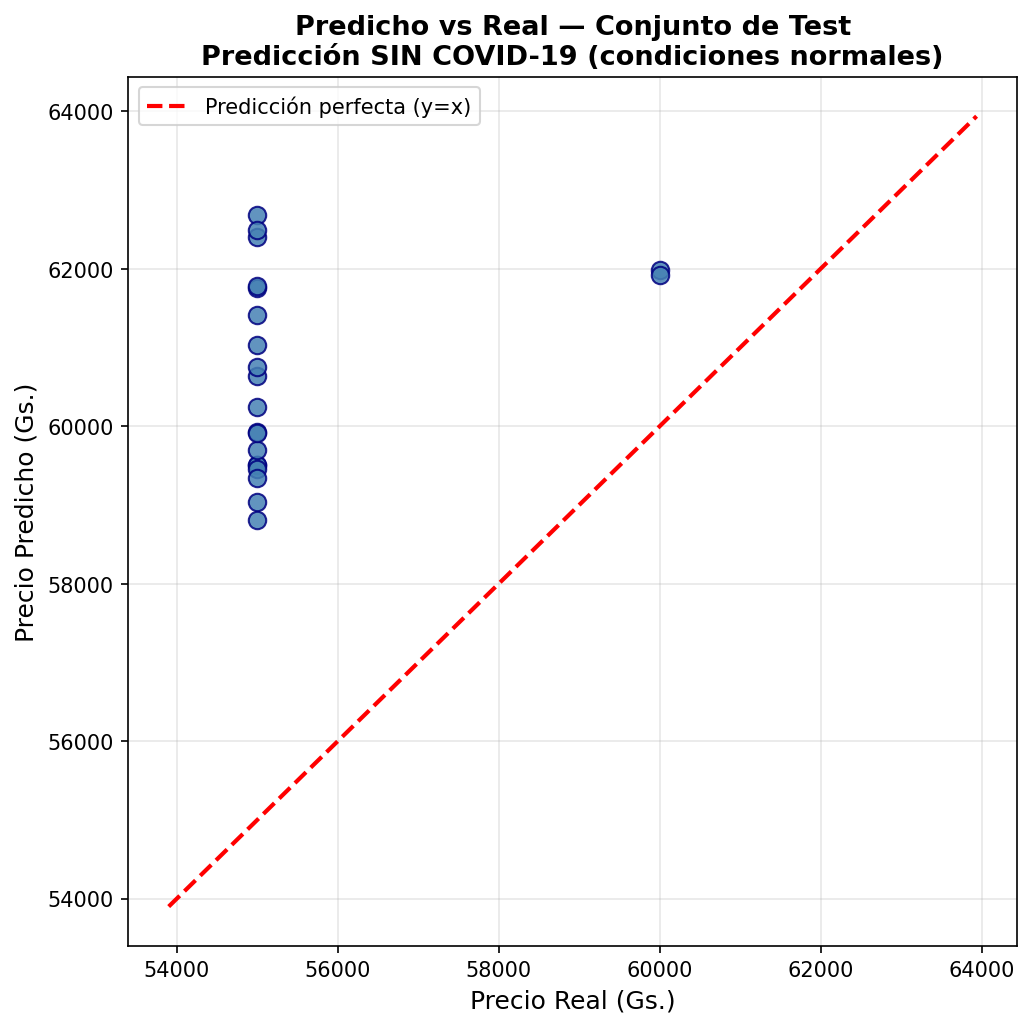
\includegraphics[width=0.7\textwidth]{predicciones/prediccion_cemento_lstm/resultados_sin_covid/final_03_scatter_test.png}
    \caption{Diagrama de dispersión: precio predicho vs.\ precio real del cemento en el conjunto de prueba.}
    \label{fig:lstm_cemento_scatter}
\end{figure}

\begin{figure}[htbp]
    \centering
    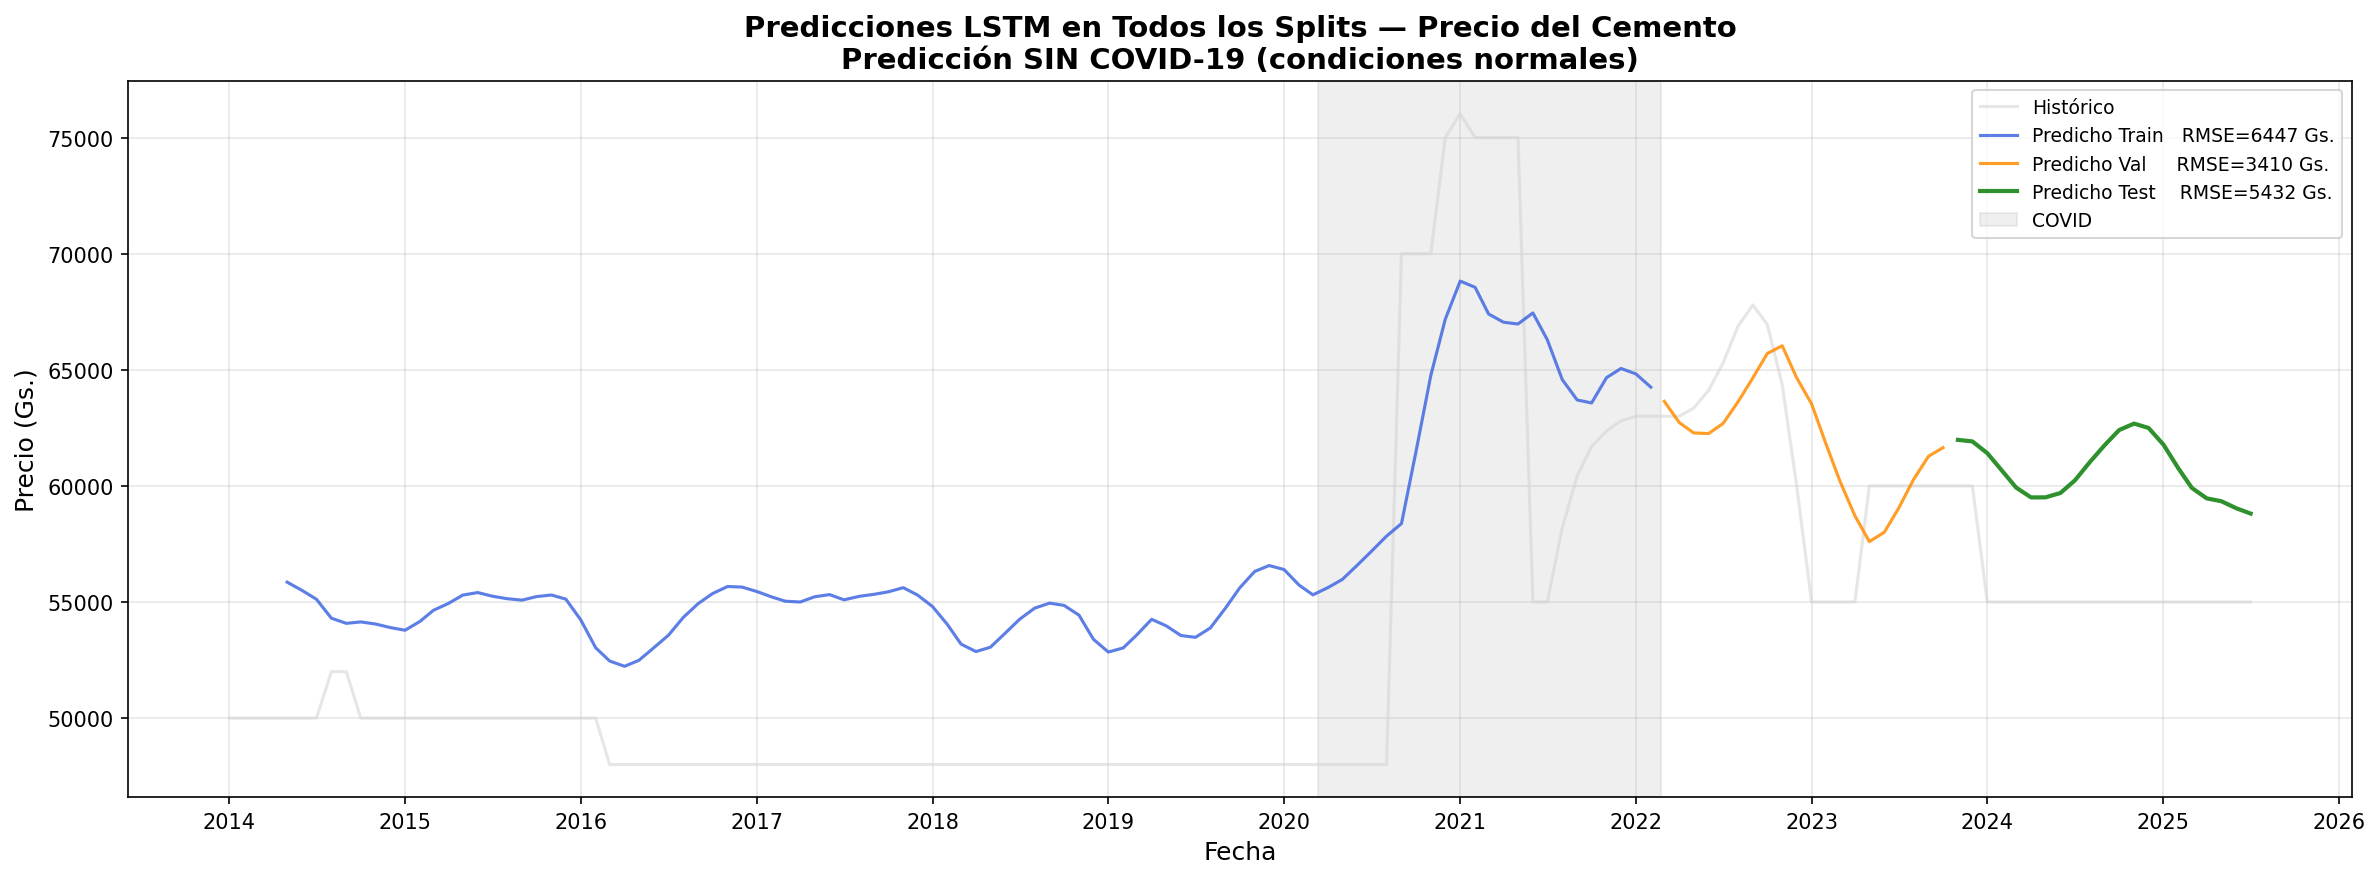
\includegraphics[width=\textwidth]{predicciones/prediccion_cemento_lstm/resultados_sin_covid/final_05_todos_splits.png}
    \caption{Predicción del modelo LSTM para cemento sobre los tres subconjuntos: entrenamiento, validación y prueba.}
    \label{fig:lstm_cemento_splits}
\end{figure}

\justify
La Figura~\ref{fig:lstm_cemento_test_serie} muestra la comparación entre los valores reales y predichos sobre el conjunto de prueba. El modelo captura la tendencia general de los precios siguiendo razonablemente bien las fluctuaciones observadas. Los puntos en el diagrama de dispersión (Figura~\ref{fig:lstm_cemento_scatter}) se agrupan en torno a la diagonal de 45°, confirmando la concordancia entre predichos y reales.

\clearpage
\subsubsection{Análisis de Residuos}

\begin{figure}[htbp]
    \centering
    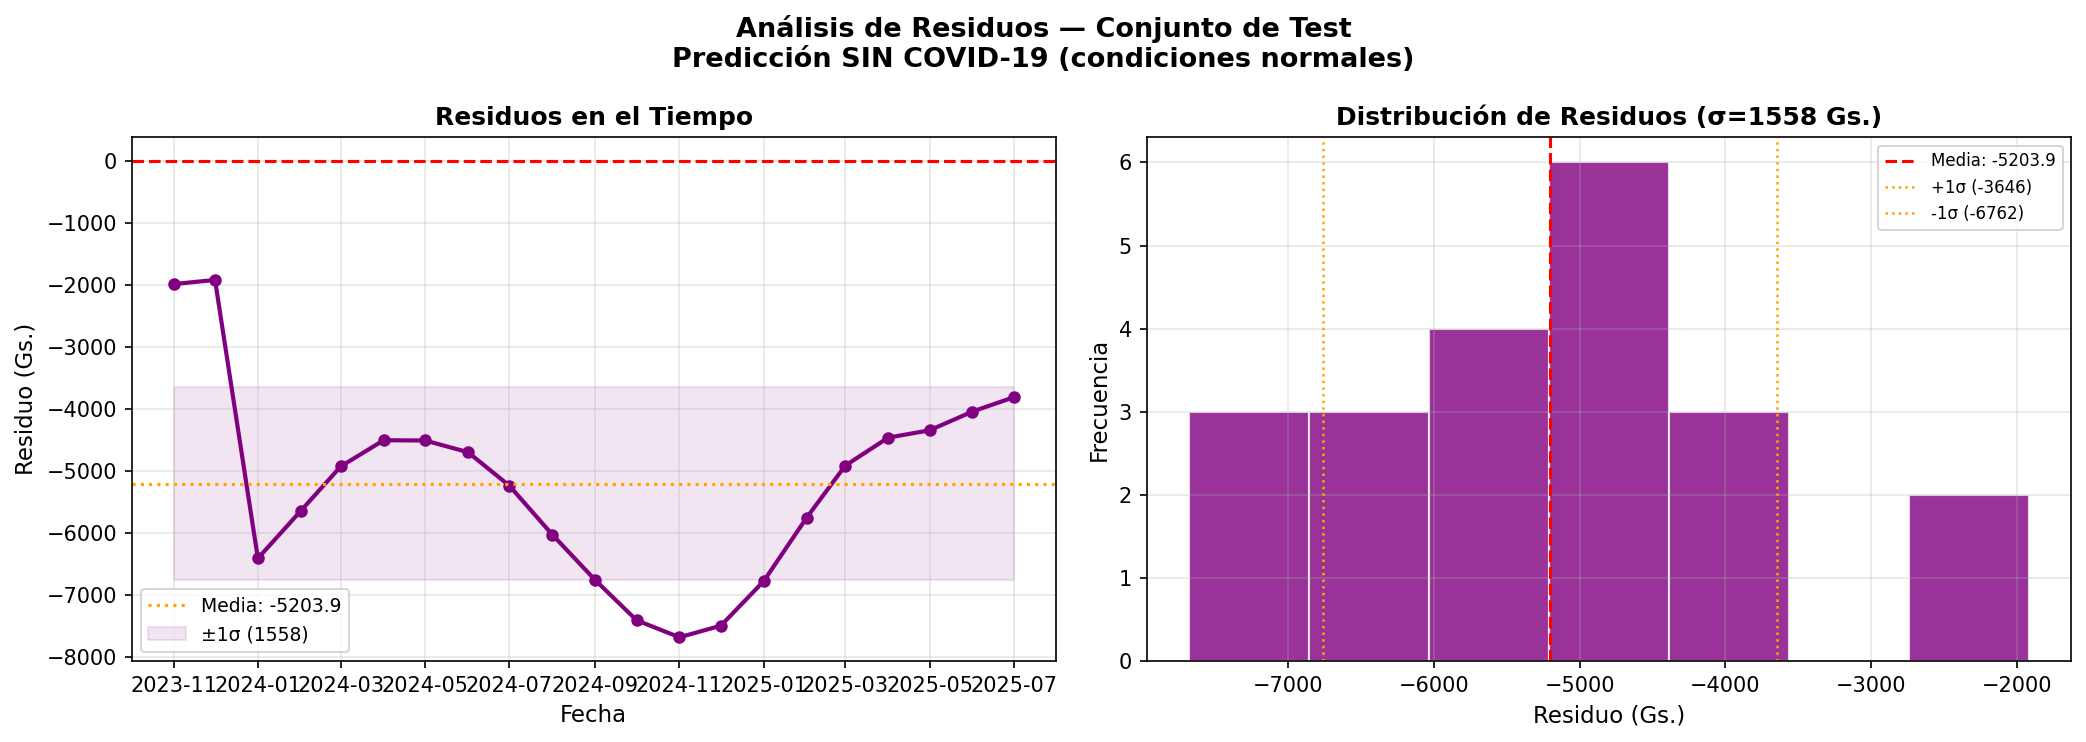
\includegraphics[width=\textwidth]{predicciones/prediccion_cemento_lstm/resultados_sin_covid/final_04_residuos.png}
    \caption{Serie temporal de residuos del modelo LSTM para cemento sobre el conjunto de prueba.}
    \label{fig:lstm_cemento_residuos}
\end{figure}

\begin{figure}[htbp]
    \centering
    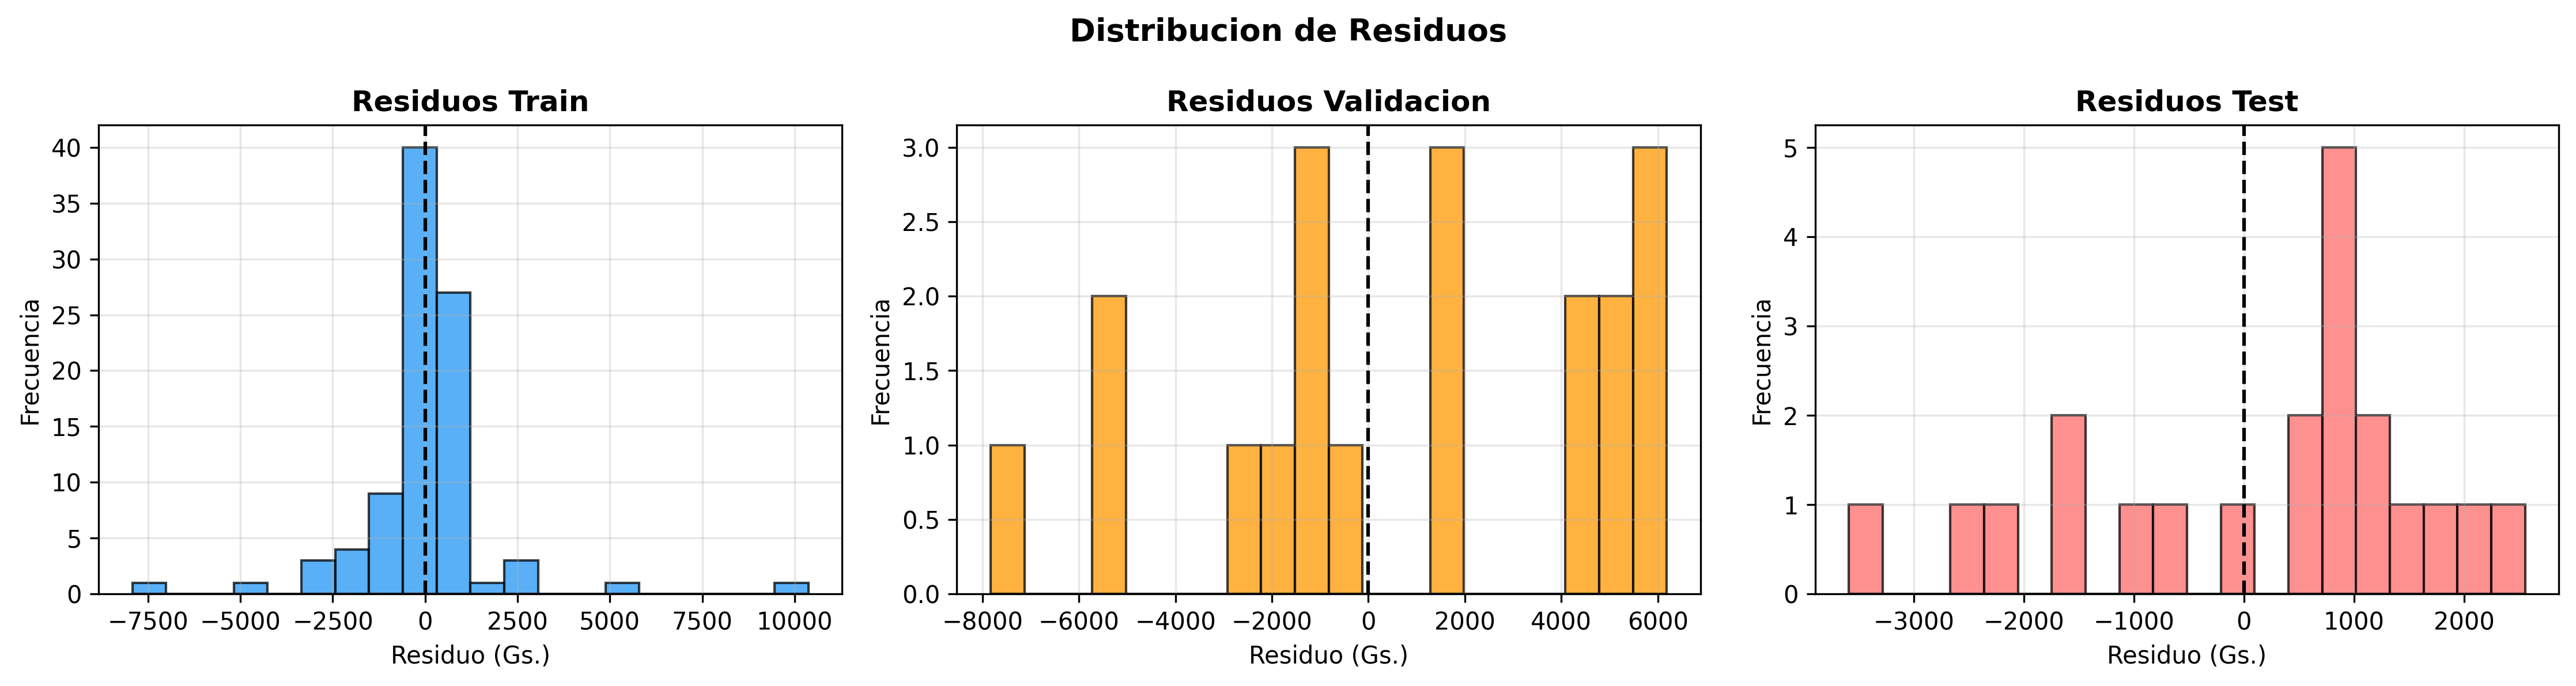
\includegraphics[width=0.75\textwidth]{predicciones/prediccion_cemento_lstm/resultados_sin_covid/residuos_histograma.png}
    \caption{Histograma de residuos del modelo LSTM para cemento.}
    \label{fig:lstm_cemento_residuos_hist}
\end{figure}

\begin{figure}[htbp]
    \centering
    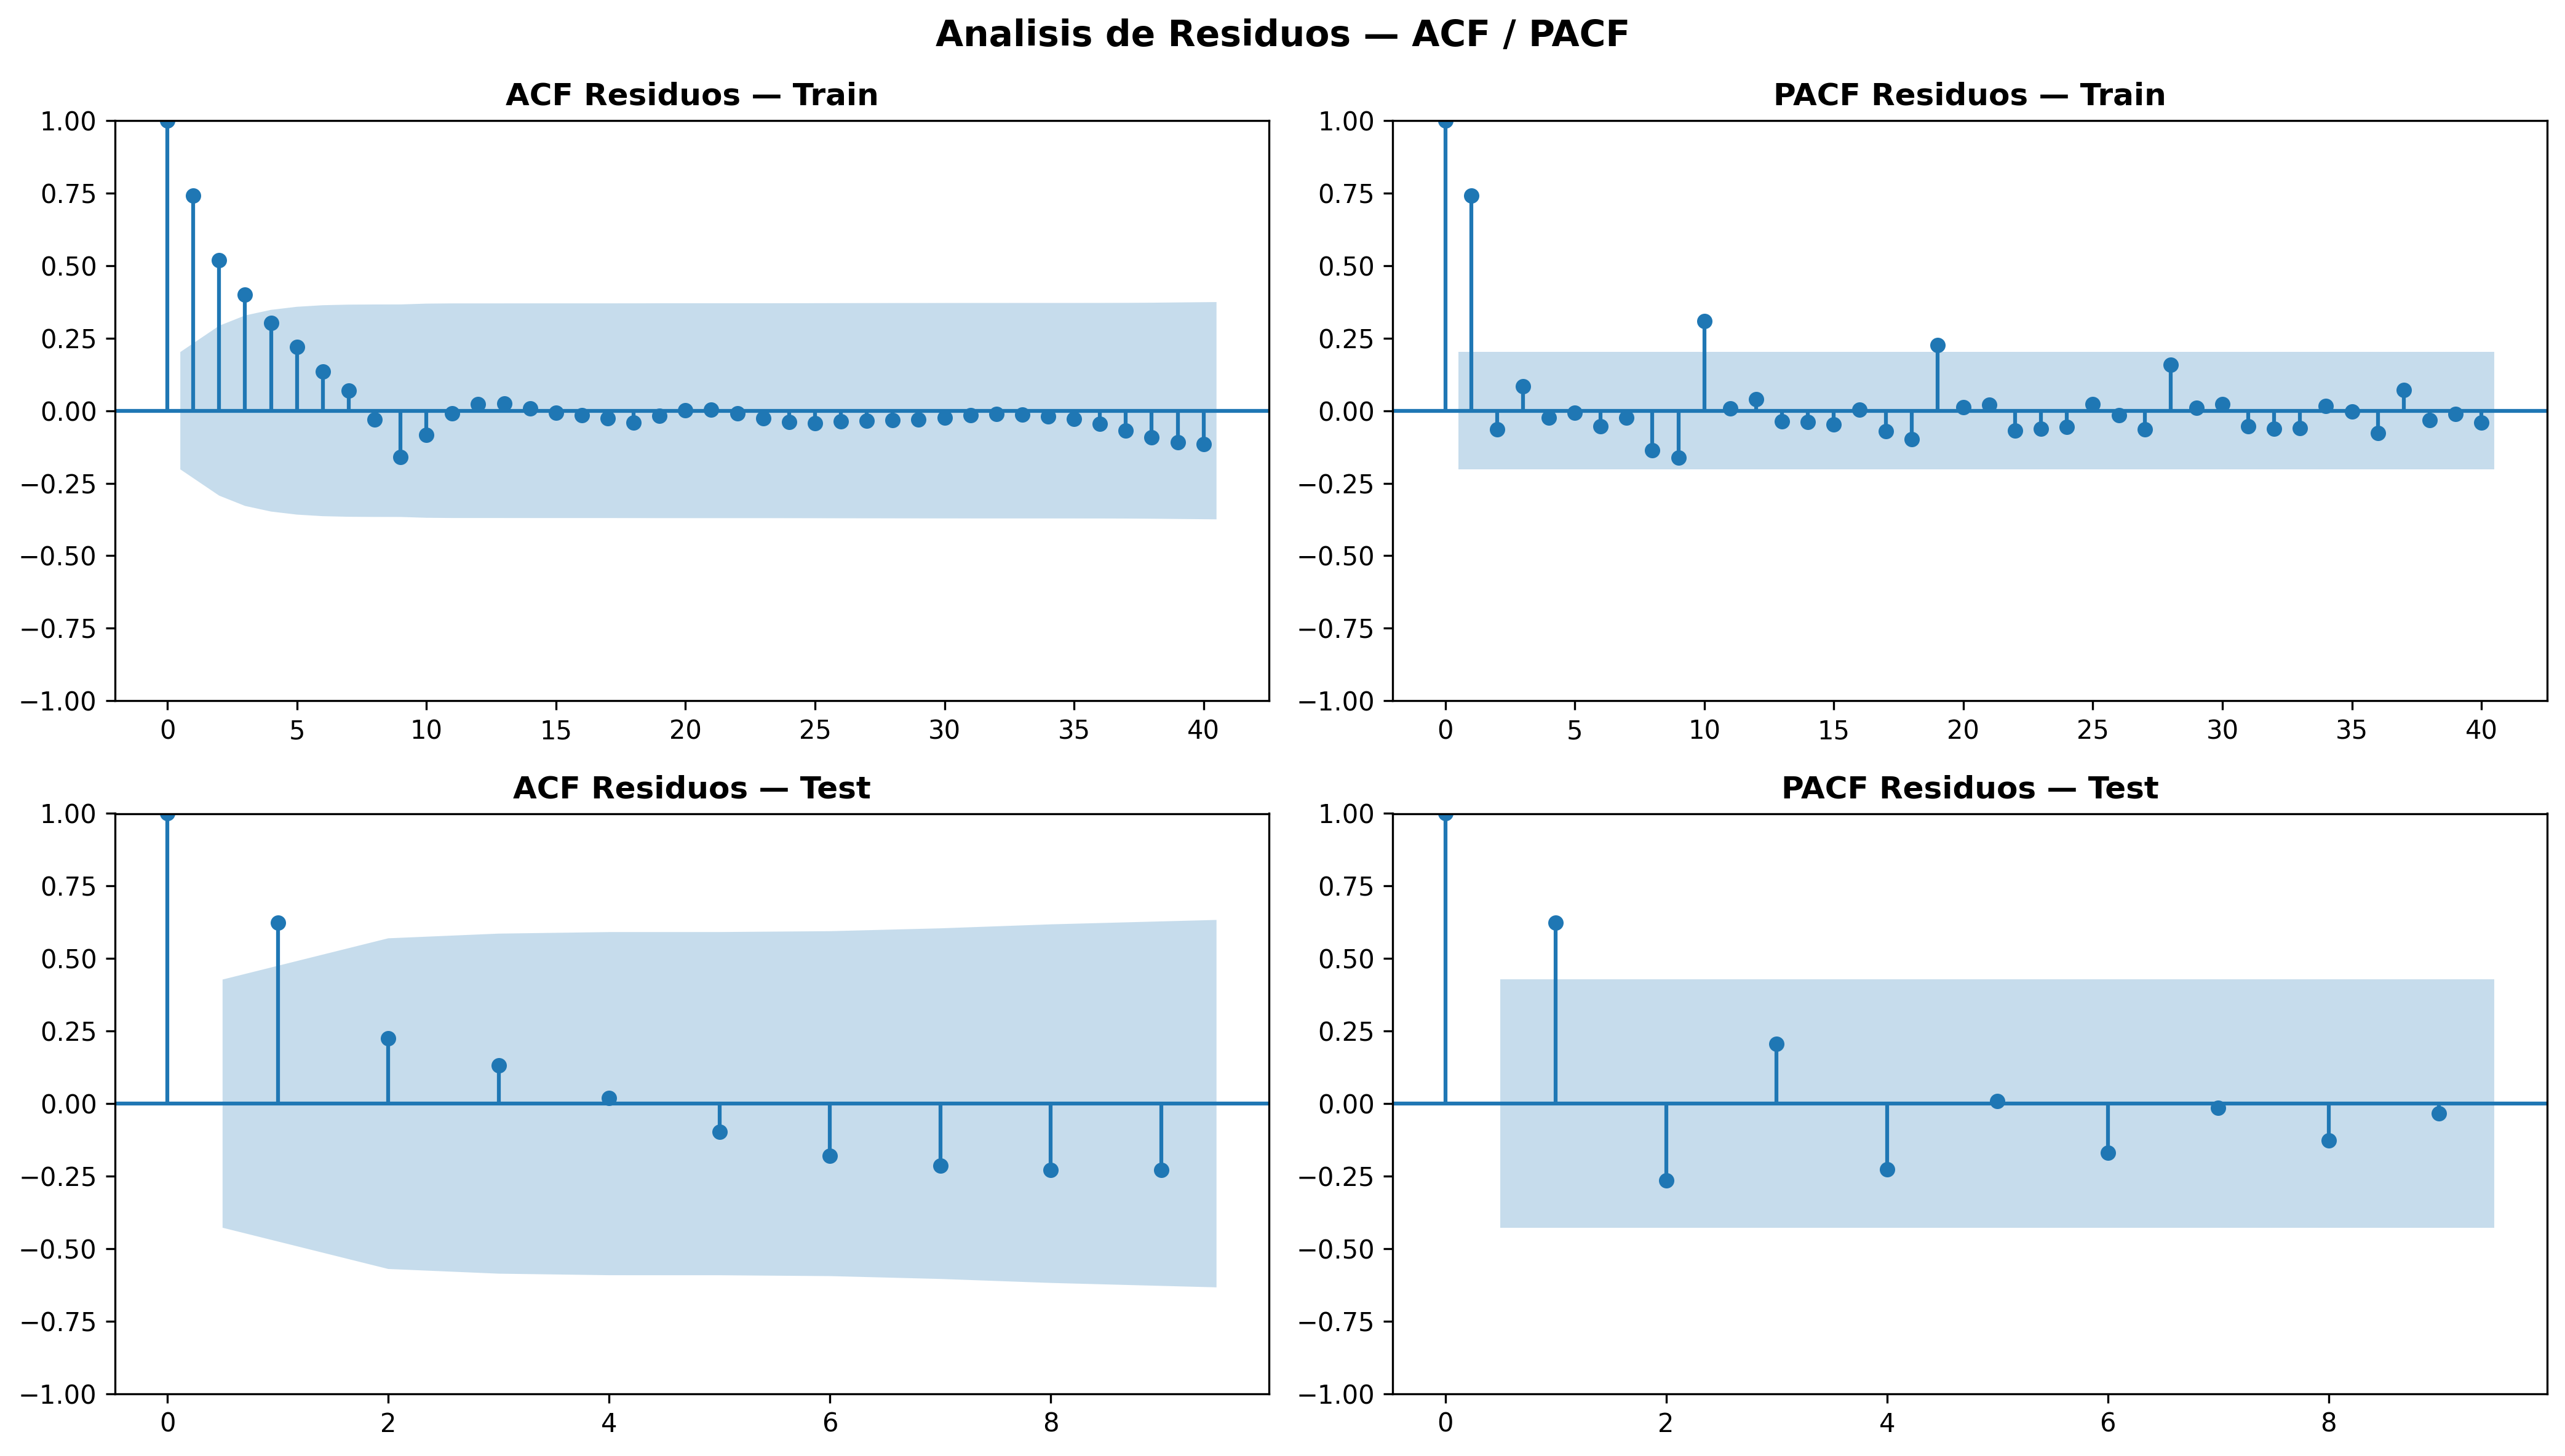
\includegraphics[width=\textwidth]{predicciones/prediccion_cemento_lstm/resultados_sin_covid/residuos_acf_pacf.png}
    \caption{ACF y PACF de los residuos del modelo LSTM para cemento.}
    \label{fig:lstm_cemento_acf_residuos}
\end{figure}

\justify
El test de Ljung-Box sobre los residuos del conjunto de prueba arrojó un $p$-valor de 0,017 con 10 rezagos y de 0,042 con 20 rezagos, ambos por debajo del umbral de 0,05. Esto indica la presencia de autocorrelación residual estadísticamente significativa, aunque los $p$-valores son cercanos al límite de significancia. Este resultado sugiere que el modelo deja alguna estructura temporal sin capturar en sus residuos, lo que debe tenerse en cuenta al interpretar los intervalos de confianza estimados por Monte Carlo Dropout.

\clearpage
\subsubsection{Pronóstico a 24 Meses --- Escenario sin Pandemia}

\justify
Se generó el pronóstico del precio del cemento para los 24 meses comprendidos entre agosto de 2025 y julio de 2027, con la variable \texttt{Cuarentena\_Covid} fijada en 0 durante todo el horizonte de predicción, simulando condiciones normales de mercado.

\begin{figure}[htbp]
    \centering
    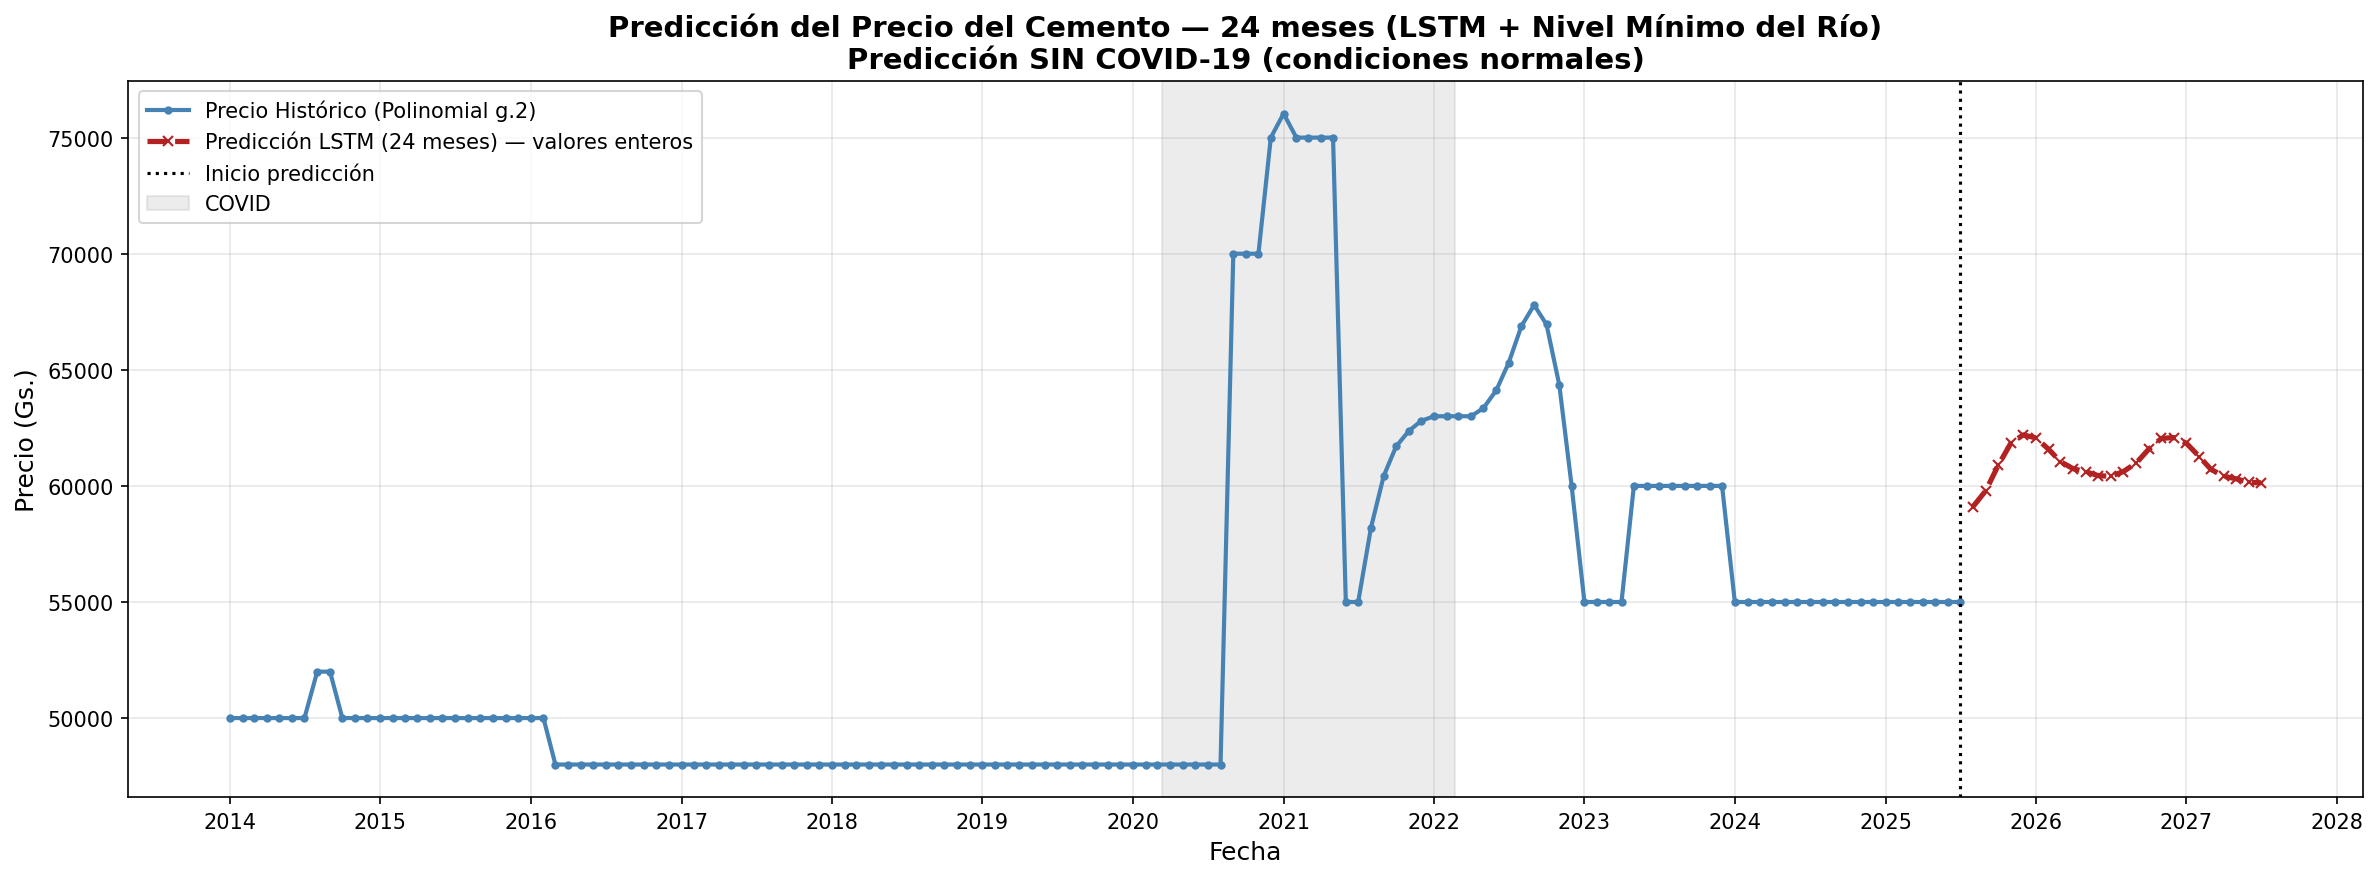
\includegraphics[width=\textwidth]{predicciones/prediccion_cemento_lstm/resultados_sin_covid/final_06_prediccion_futura_completa.png}
    \caption{Pronóstico LSTM a 24 meses del precio del cemento --- escenario sin pandemia, con intervalos de confianza al 95\,\%.}
    \label{fig:lstm_cemento_pred_sin_covid}
\end{figure}

\begin{figure}[htbp]
    \centering
    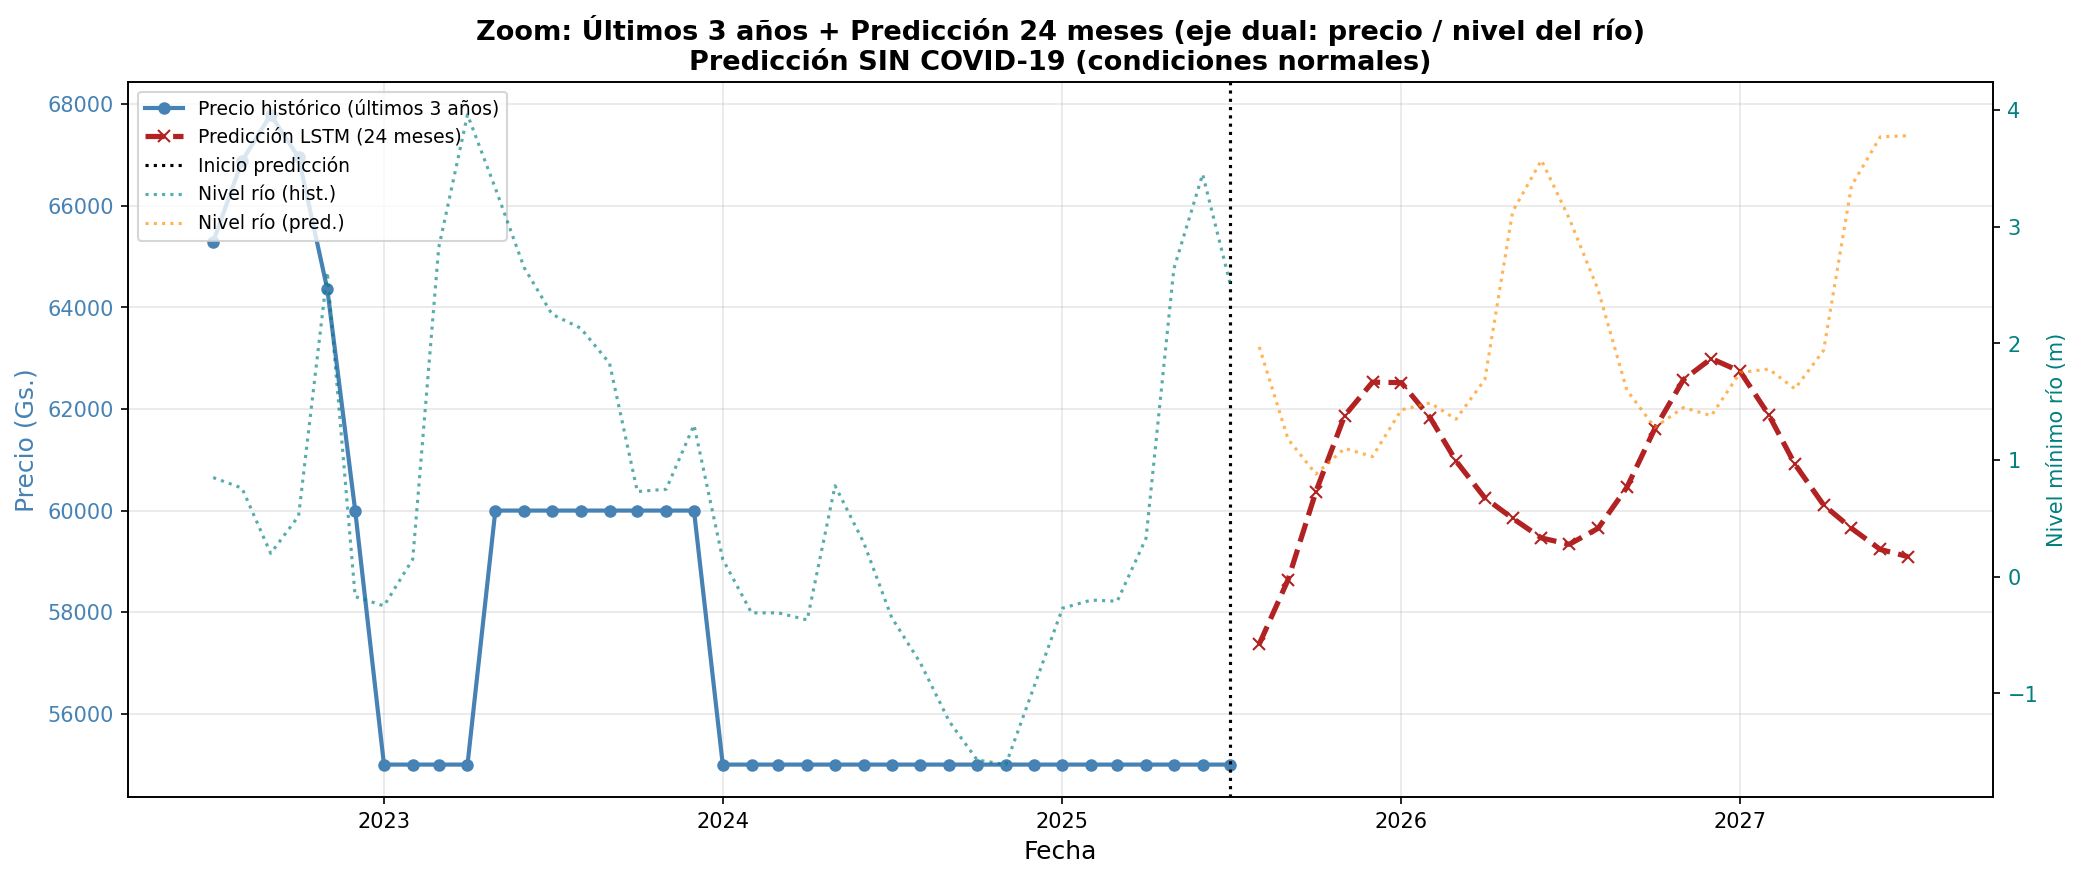
\includegraphics[width=\textwidth]{predicciones/prediccion_cemento_lstm/resultados_sin_covid/final_07_prediccion_zoom_dual.png}
    \caption{Detalle de la transición entre datos históricos y pronóstico LSTM del cemento --- escenario sin pandemia.}
    \label{fig:lstm_cemento_zoom_sin_covid}
\end{figure}

\begin{figure}[htbp]
    \centering
    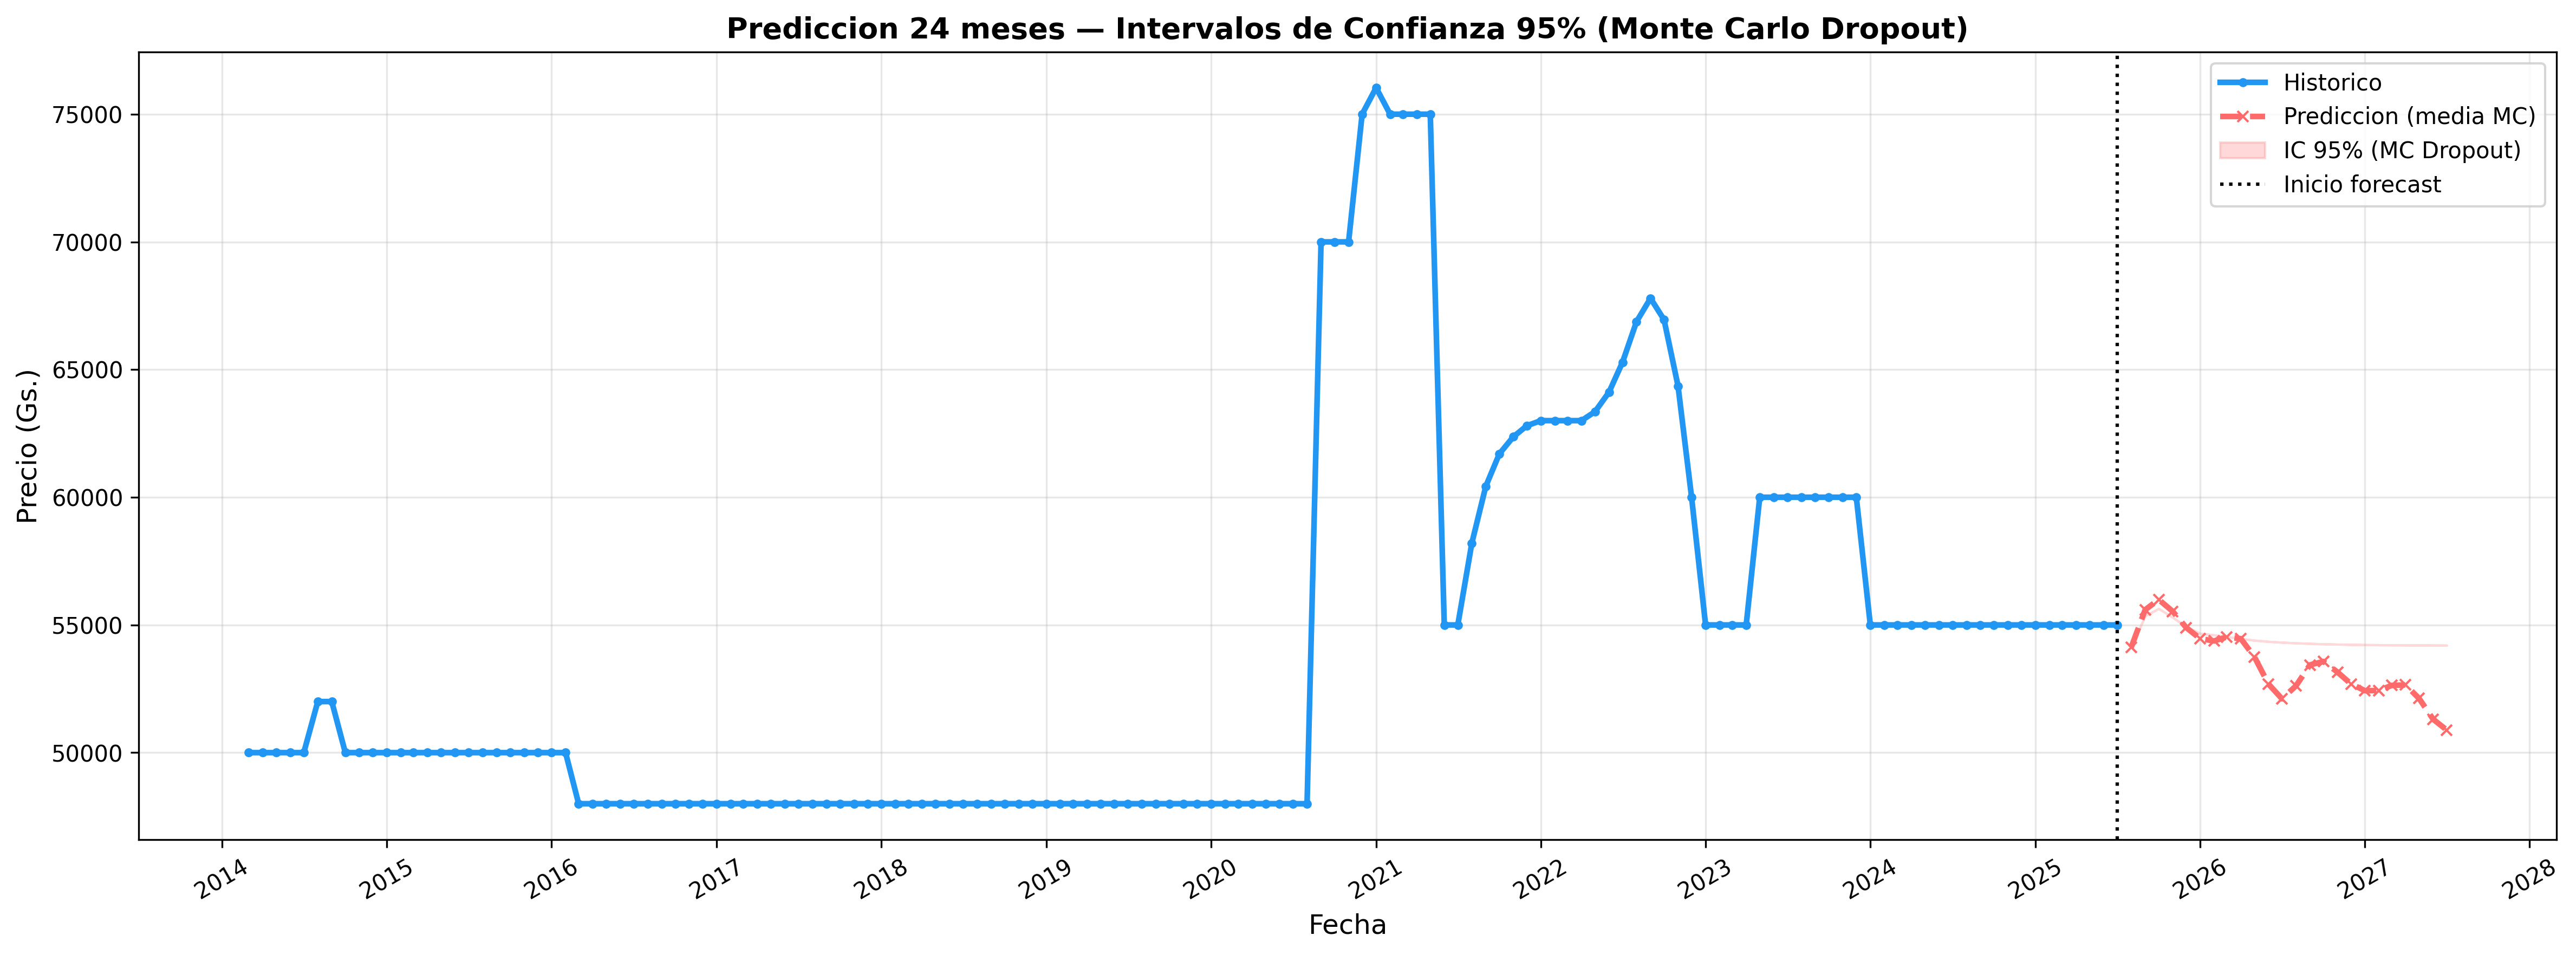
\includegraphics[width=\textwidth]{predicciones/prediccion_cemento_lstm/resultados_sin_covid/forecast_ic_monte_carlo.png}
    \caption{Intervalo de confianza Monte Carlo Dropout del pronóstico LSTM para cemento --- escenario sin pandemia.}
    \label{fig:lstm_cemento_ic_mc_sin_covid}
\end{figure}

\justify
Bajo el escenario sin pandemia, el rango de precios predicho se sitúa entre Gs.~50.888 y Gs.~55.996 a lo largo del horizonte de 24 meses, reflejando una tendencia estable con leve tendencia descendente a partir del primer año de proyección.

\clearpage
\subsubsection{Pronóstico a 24 Meses --- Escenario con Efecto Pandémico}

\justify
En este escenario, el mismo modelo entrenado se utilizó para generar el pronóstico con la variable \texttt{Cuarentena\_Covid} activada (valor 1) durante todo el horizonte de predicción. Este escenario hipotético permite evaluar cómo el modelo LSTM responde ante disrupciones prolongadas de tipo pandémico.

\begin{figure}[htbp]
    \centering
    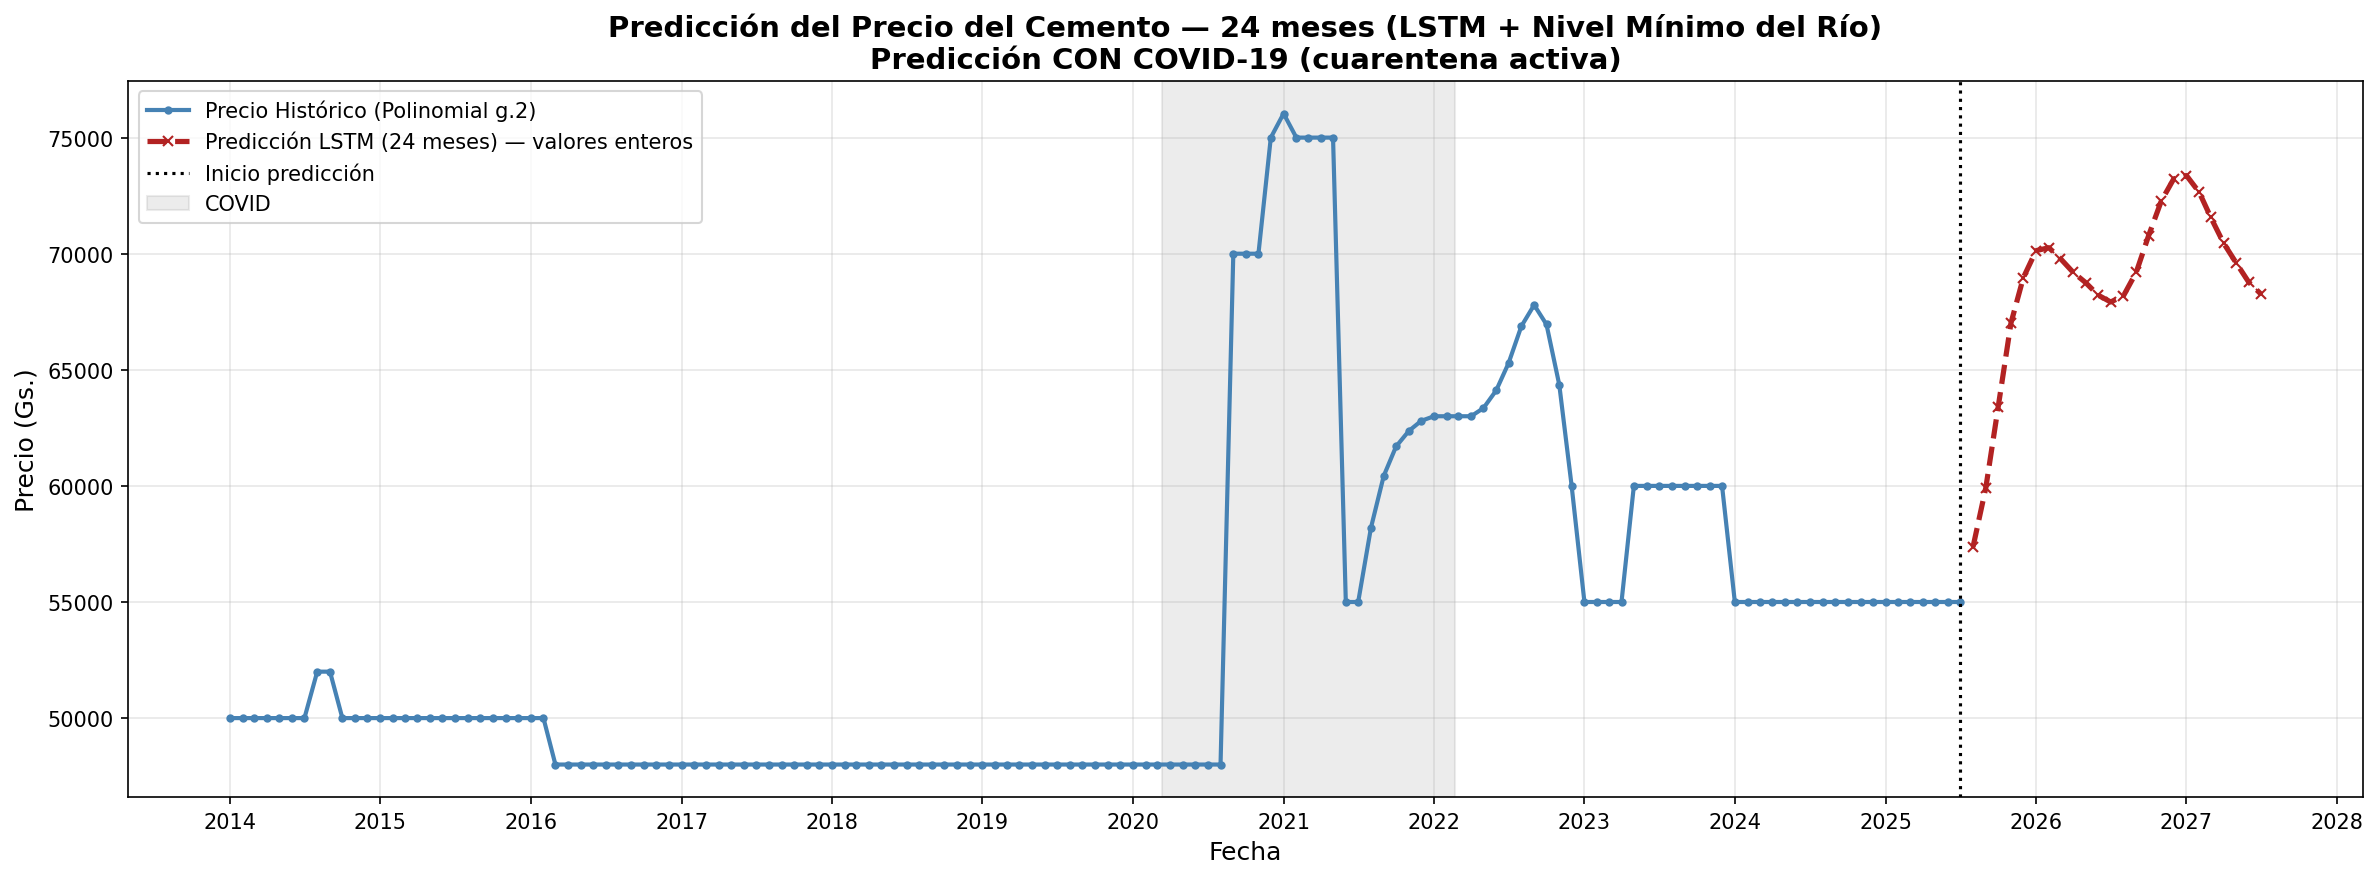
\includegraphics[width=\textwidth]{predicciones/prediccion_cemento_lstm/resultados_con_covid/final_06_prediccion_futura_completa.png}
    \caption{Pronóstico LSTM a 24 meses del precio del cemento --- escenario con efecto pandémico, con intervalos de confianza al 95\,\%.}
    \label{fig:lstm_cemento_pred_con_covid}
\end{figure}

\begin{figure}[htbp]
    \centering
    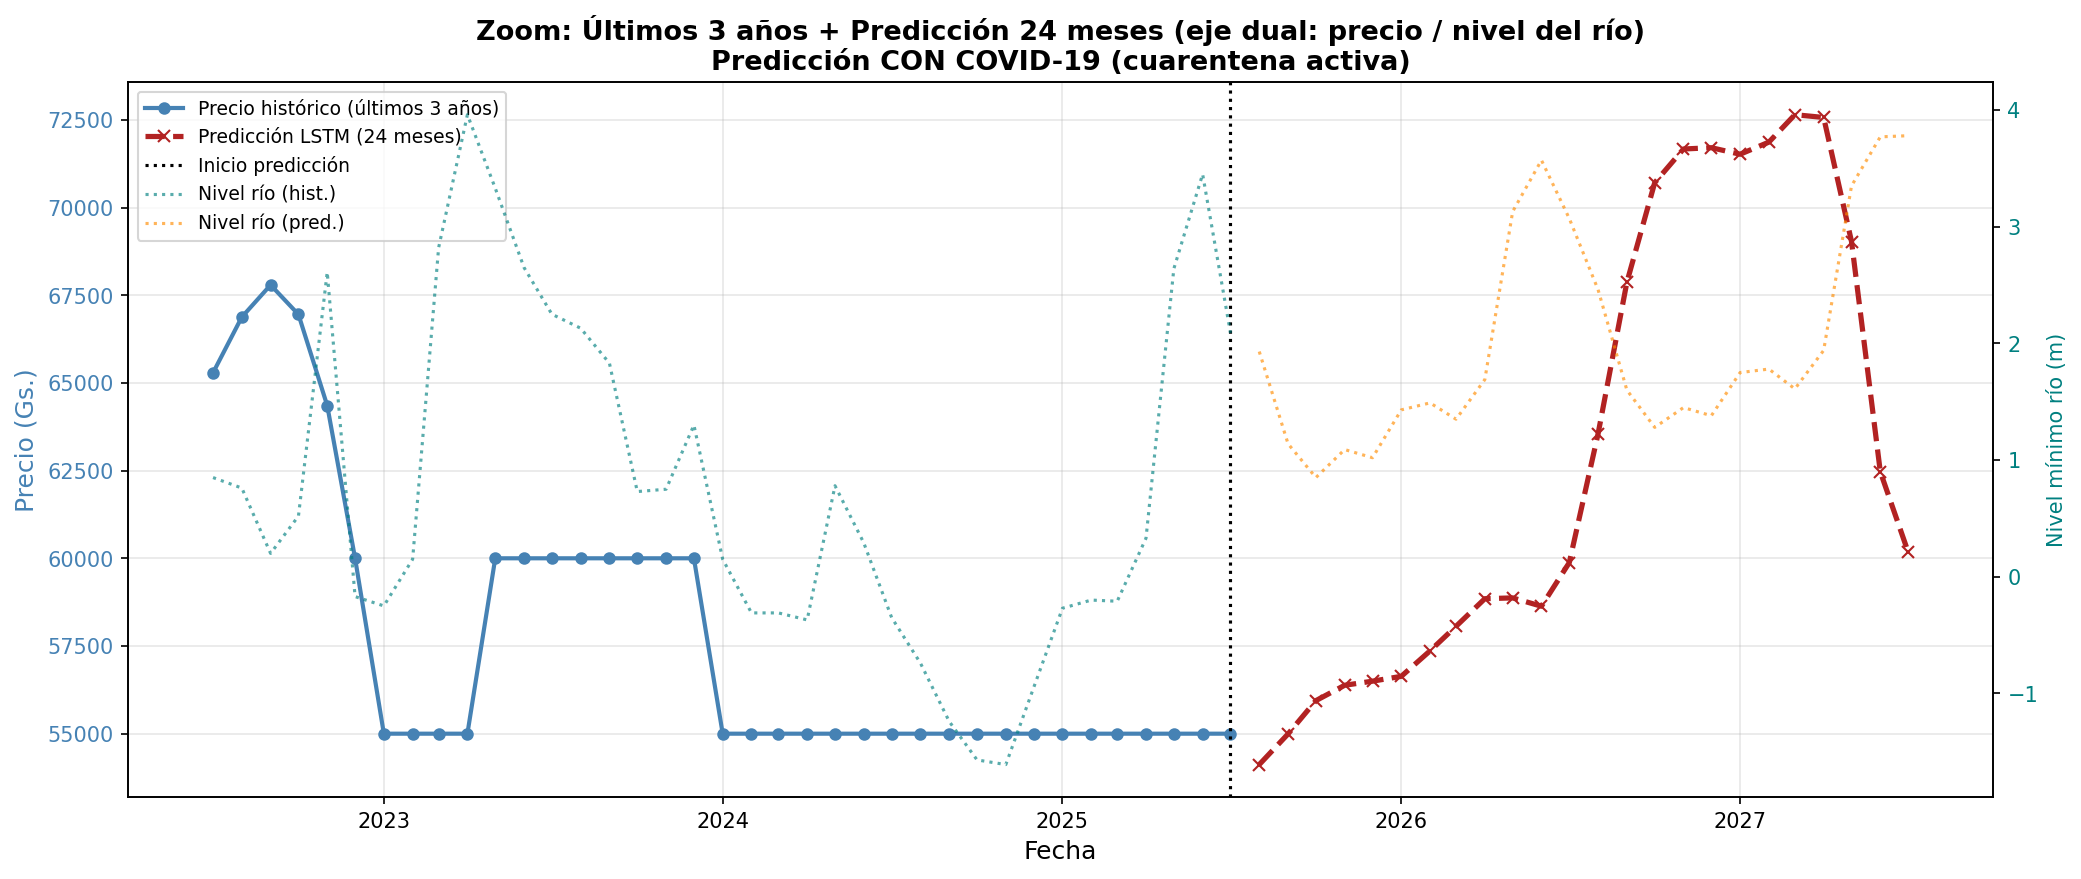
\includegraphics[width=\textwidth]{predicciones/prediccion_cemento_lstm/resultados_con_covid/final_07_prediccion_zoom_dual.png}
    \caption{Detalle de la transición entre datos históricos y pronóstico LSTM del cemento --- escenario con efecto pandémico.}
    \label{fig:lstm_cemento_zoom_con_covid}
\end{figure}

\begin{figure}[htbp]
    \centering
    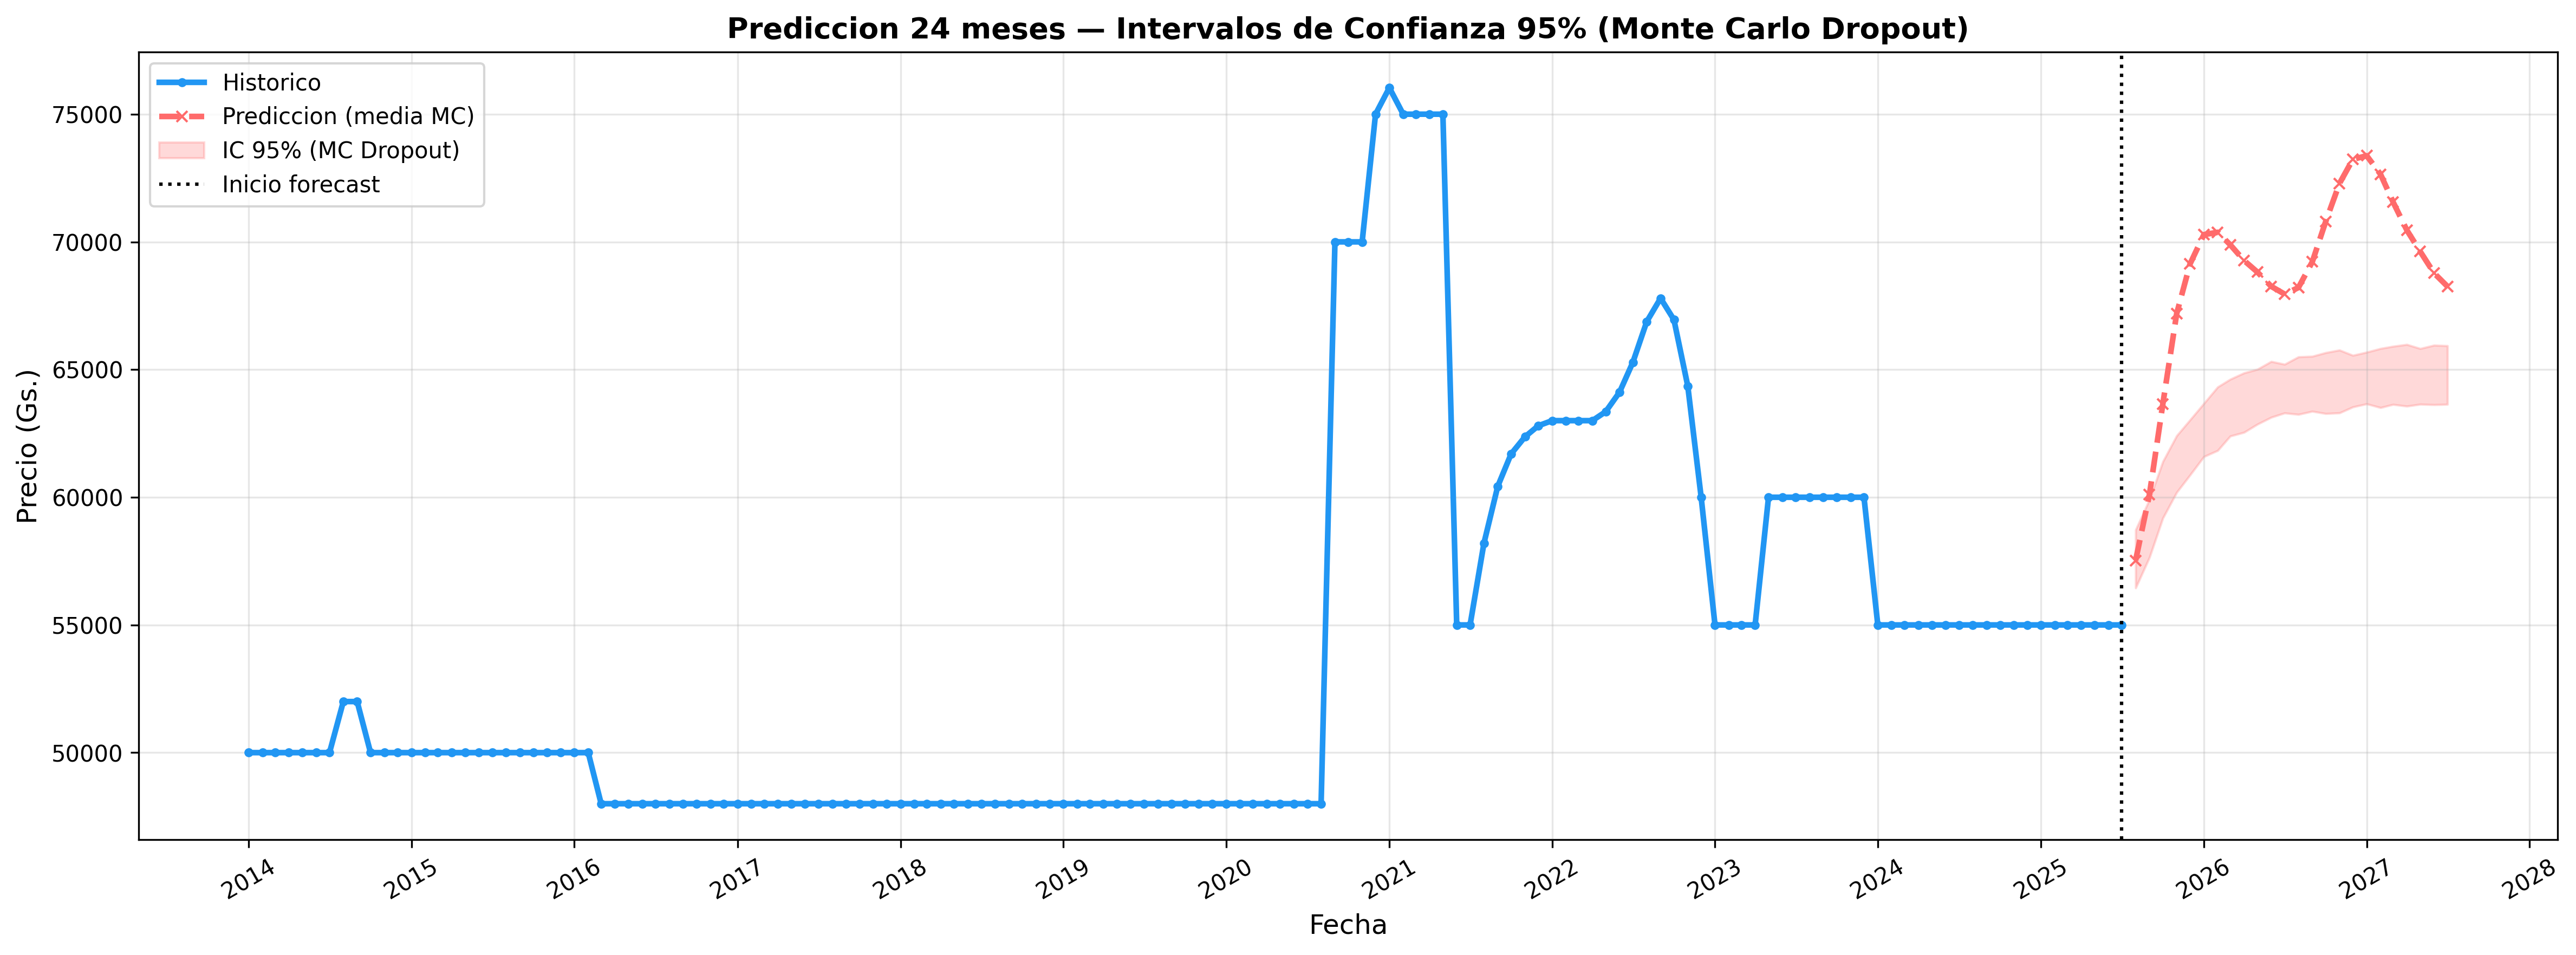
\includegraphics[width=\textwidth]{predicciones/prediccion_cemento_lstm/resultados_con_covid/forecast_ic_monte_carlo.png}
    \caption{Intervalo de confianza Monte Carlo Dropout del pronóstico LSTM para cemento --- escenario con efecto pandémico.}
    \label{fig:lstm_cemento_ic_mc_con_covid}
\end{figure}

\justify
Bajo el escenario con efecto pandémico, el rango de precios predicho se sitúa entre Gs.~54.119 y Gs.~72.646, considerablemente más elevado y con mayor dispersión que el escenario sin pandemia. La diferencia entre ambos escenarios revela que el modelo LSTM asigna un efecto alcista significativo a la variable de cuarentena: el precio máximo predicho pasa de Gs.~55.996 (sin pandemia) a Gs.~72.646 (con pandemia), un incremento del 29,7\,\% en el límite superior del rango. Este comportamiento es consistente con lo observado durante la pandemia real de 2020--2021, donde las disrupciones en la cadena de suministro provocaron aumentos sostenidos en los precios del cemento.

% ============================================================
%  LADRILLO
% ============================================================
\clearpage
\subsection{Predicción del Precio del Ladrillo}

\justify
Para el ladrillo, la búsqueda de hiperparámetros con Optuna identificó arquitecturas diferentes para cada escenario. El escenario sin pandemia fue optimizado con 261 pruebas durante 480,9 minutos y convergió a una arquitectura LSTM bidireccional; el escenario con pandemia, con una sola prueba de configuración, seleccionó una arquitectura unidireccional más compacta. Dado que los modelos son distintos, cada escenario se presenta con su propia descripción completa: hiperparámetros, entrenamiento, evaluación y pronóstico.

\subsubsection{Análisis Exploratorio de la Serie}

\begin{figure}[htbp]
    \centering
    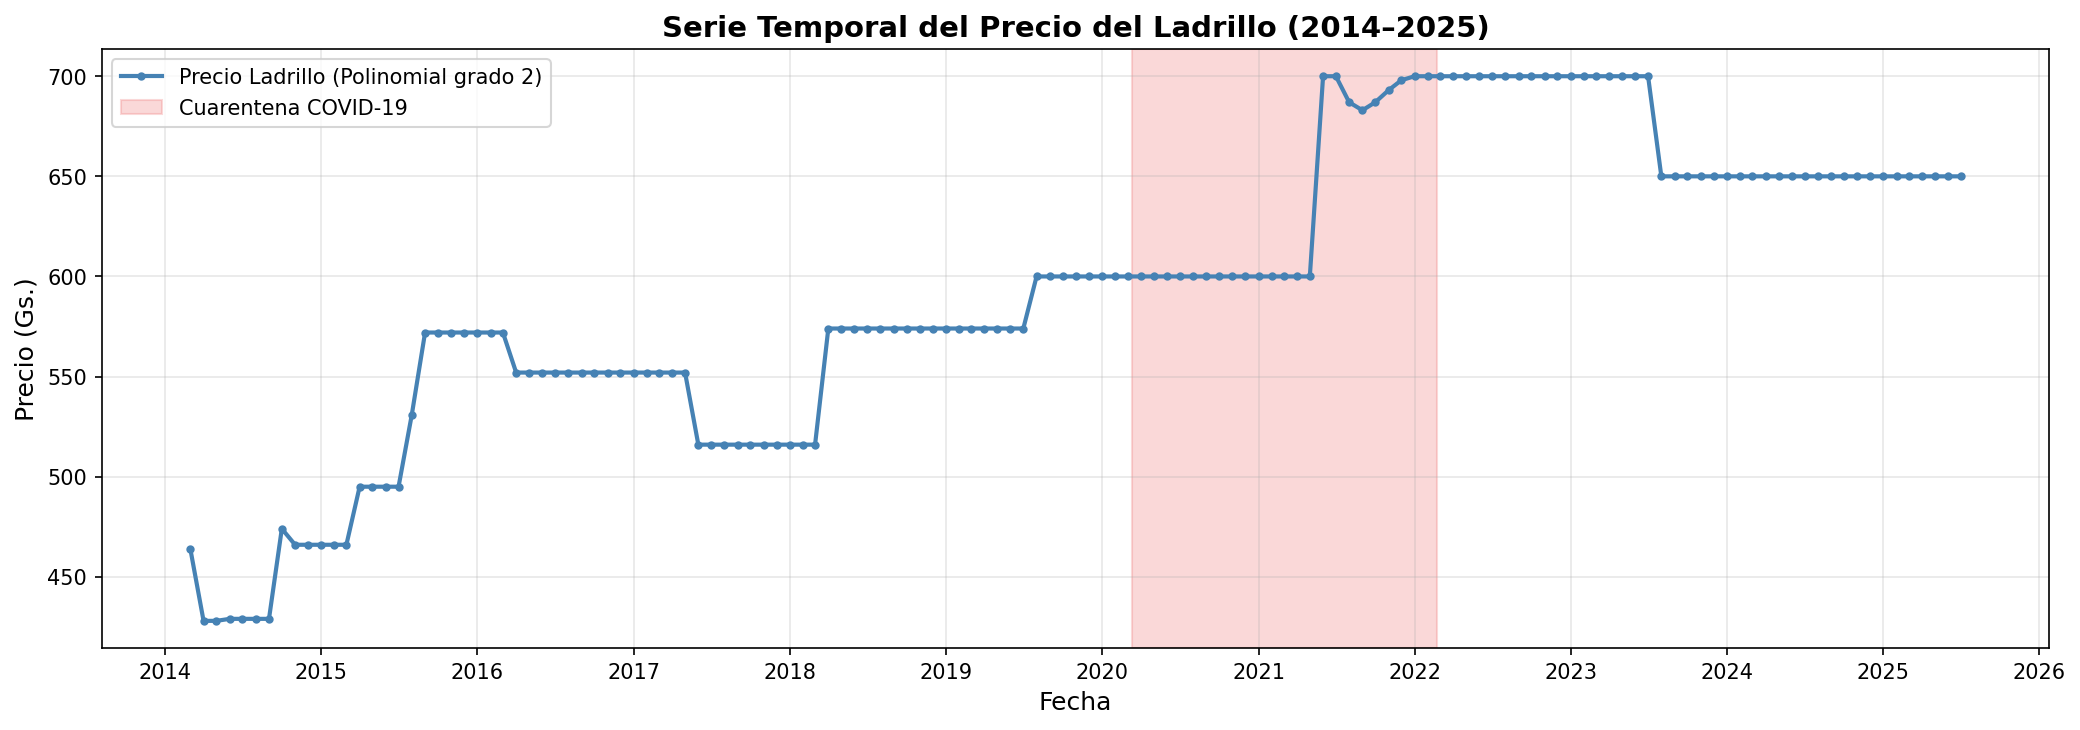
\includegraphics[width=\textwidth]{predicciones/prediccion_ladrillo_lstm/resultados_sin_covid/eda_01_serie_precios_ladrillo.png}
    \caption{Serie histórica mensual del precio del ladrillo (Gs.), período 2014--2025.}
    \label{fig:lstm_ladrillo_eda_serie}
\end{figure}

\begin{figure}[htbp]
    \centering
    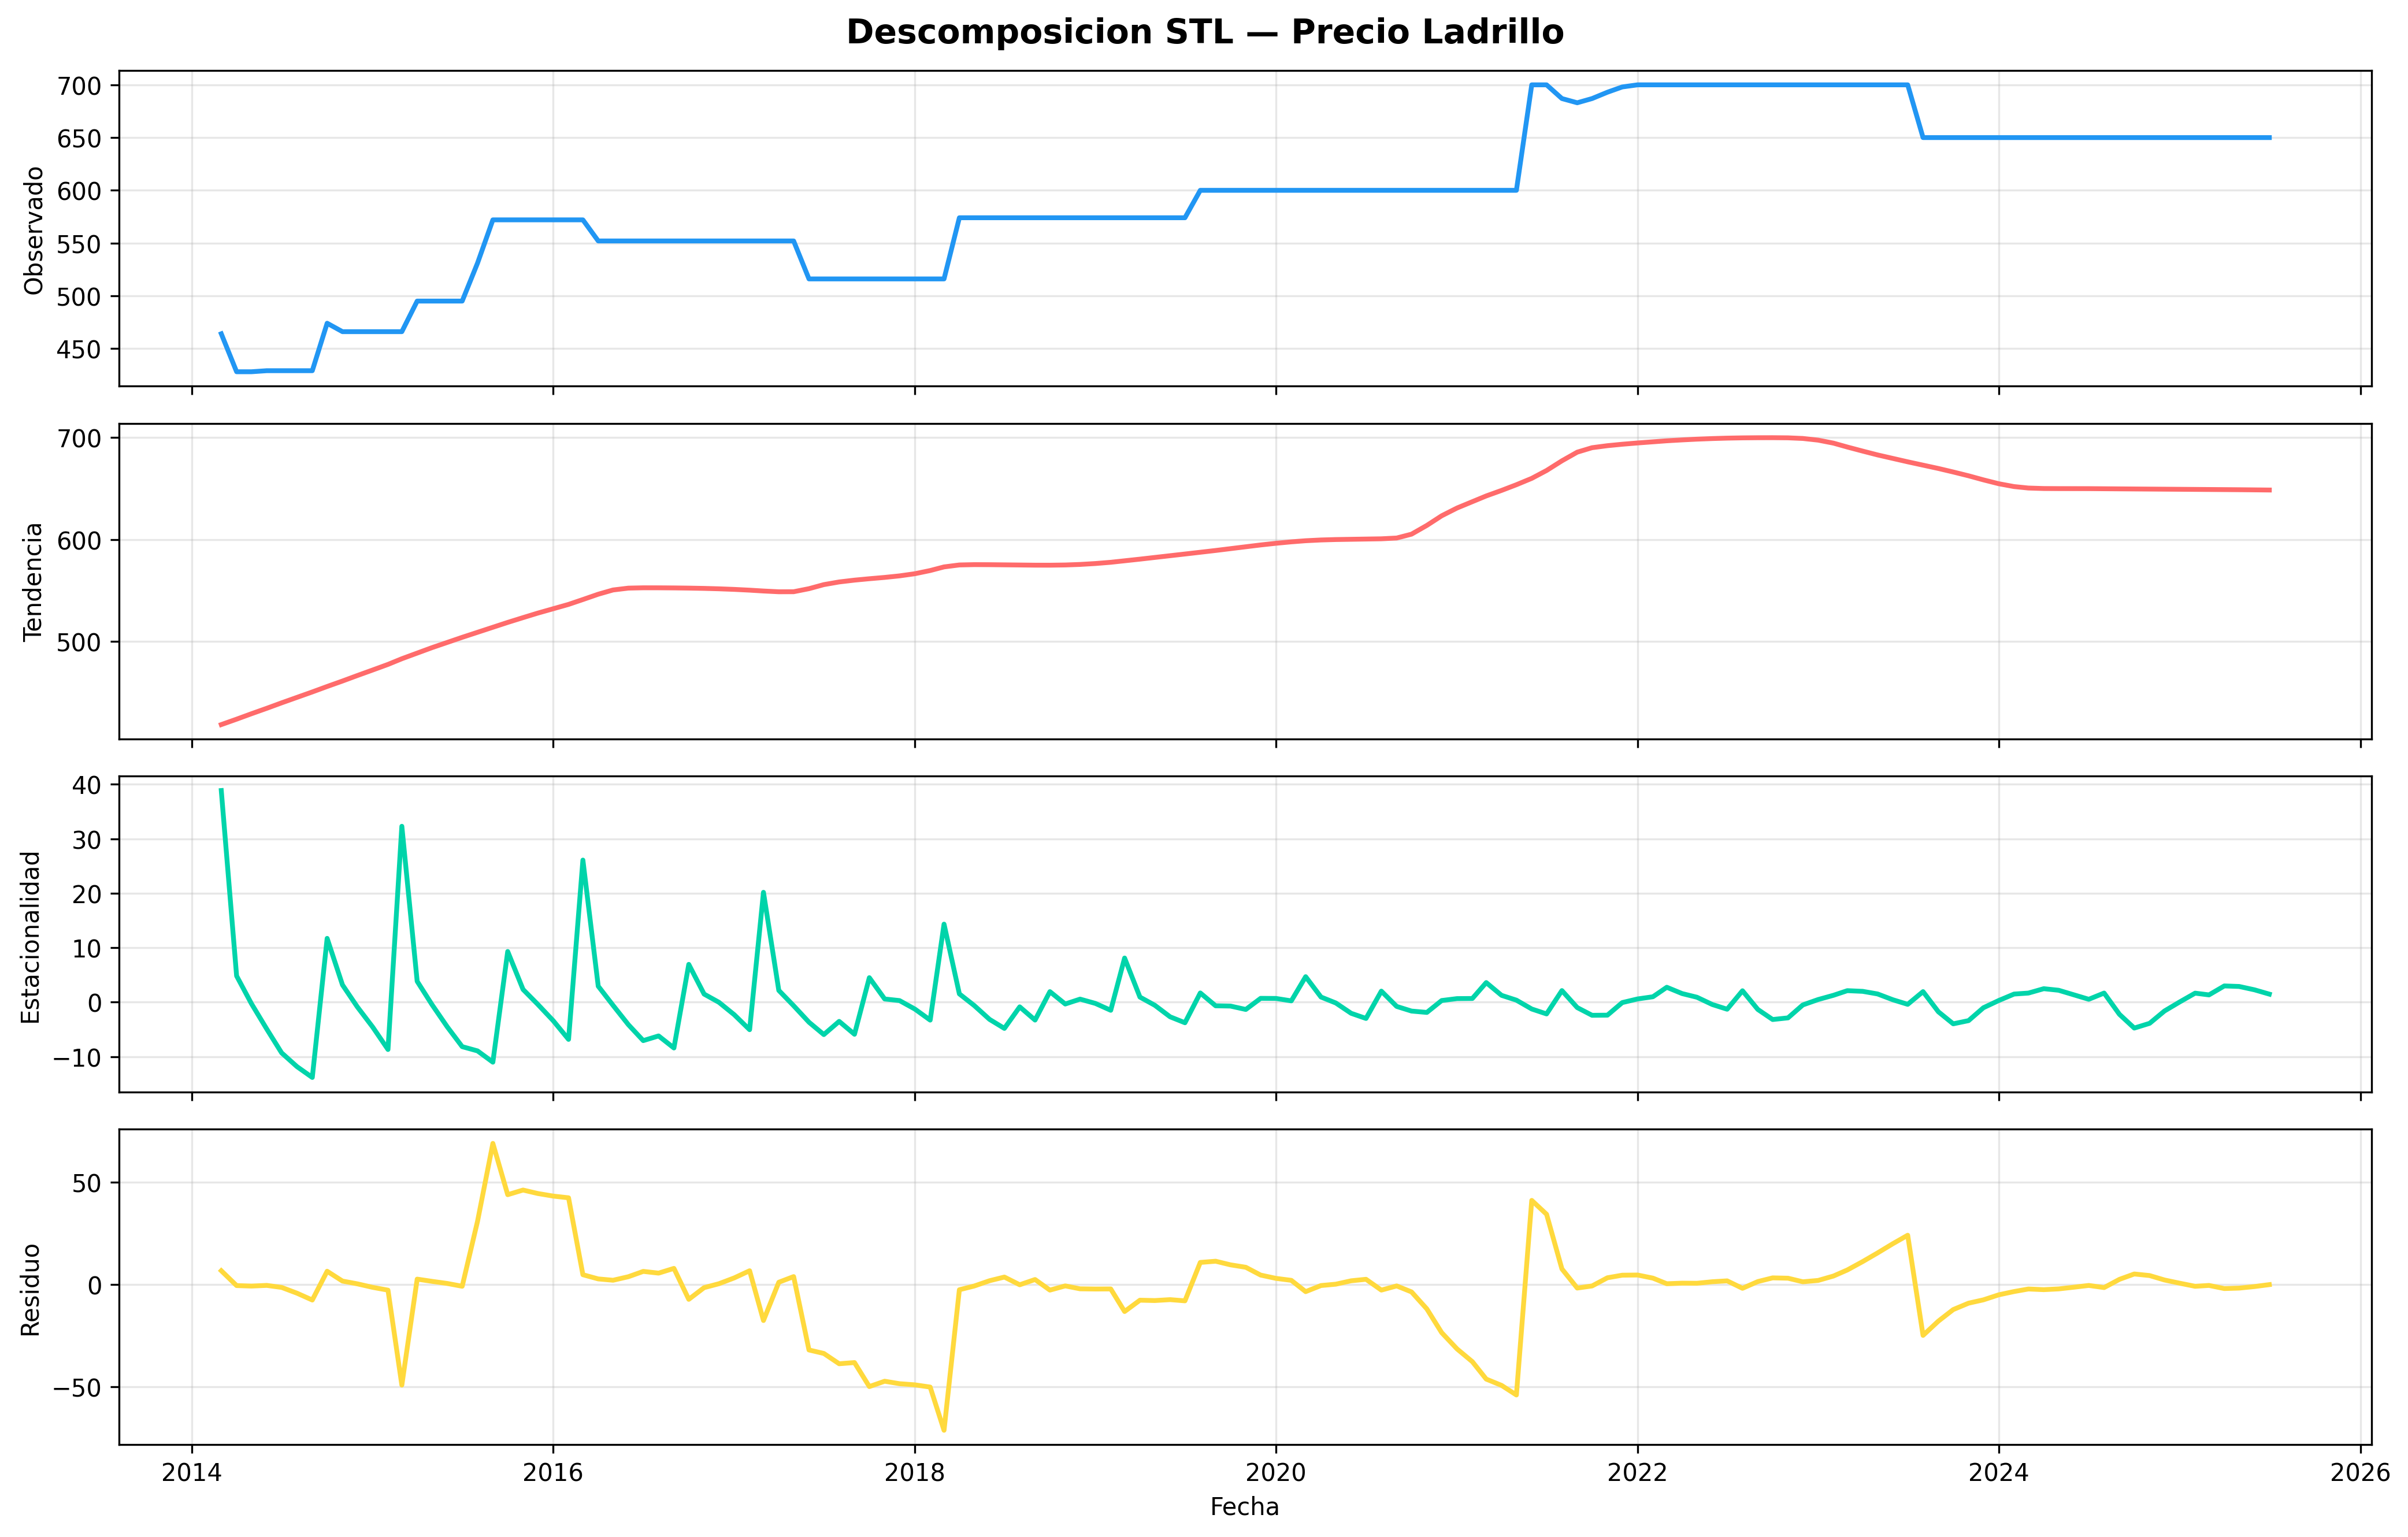
\includegraphics[width=\textwidth]{predicciones/prediccion_ladrillo_lstm/resultados_sin_covid/eda_stl_decomposition.png}
    \caption{Descomposición STL de la serie del precio del ladrillo: tendencia, estacionalidad y residuo.}
    \label{fig:lstm_ladrillo_eda_stl}
\end{figure}

\begin{figure}[htbp]
    \centering
    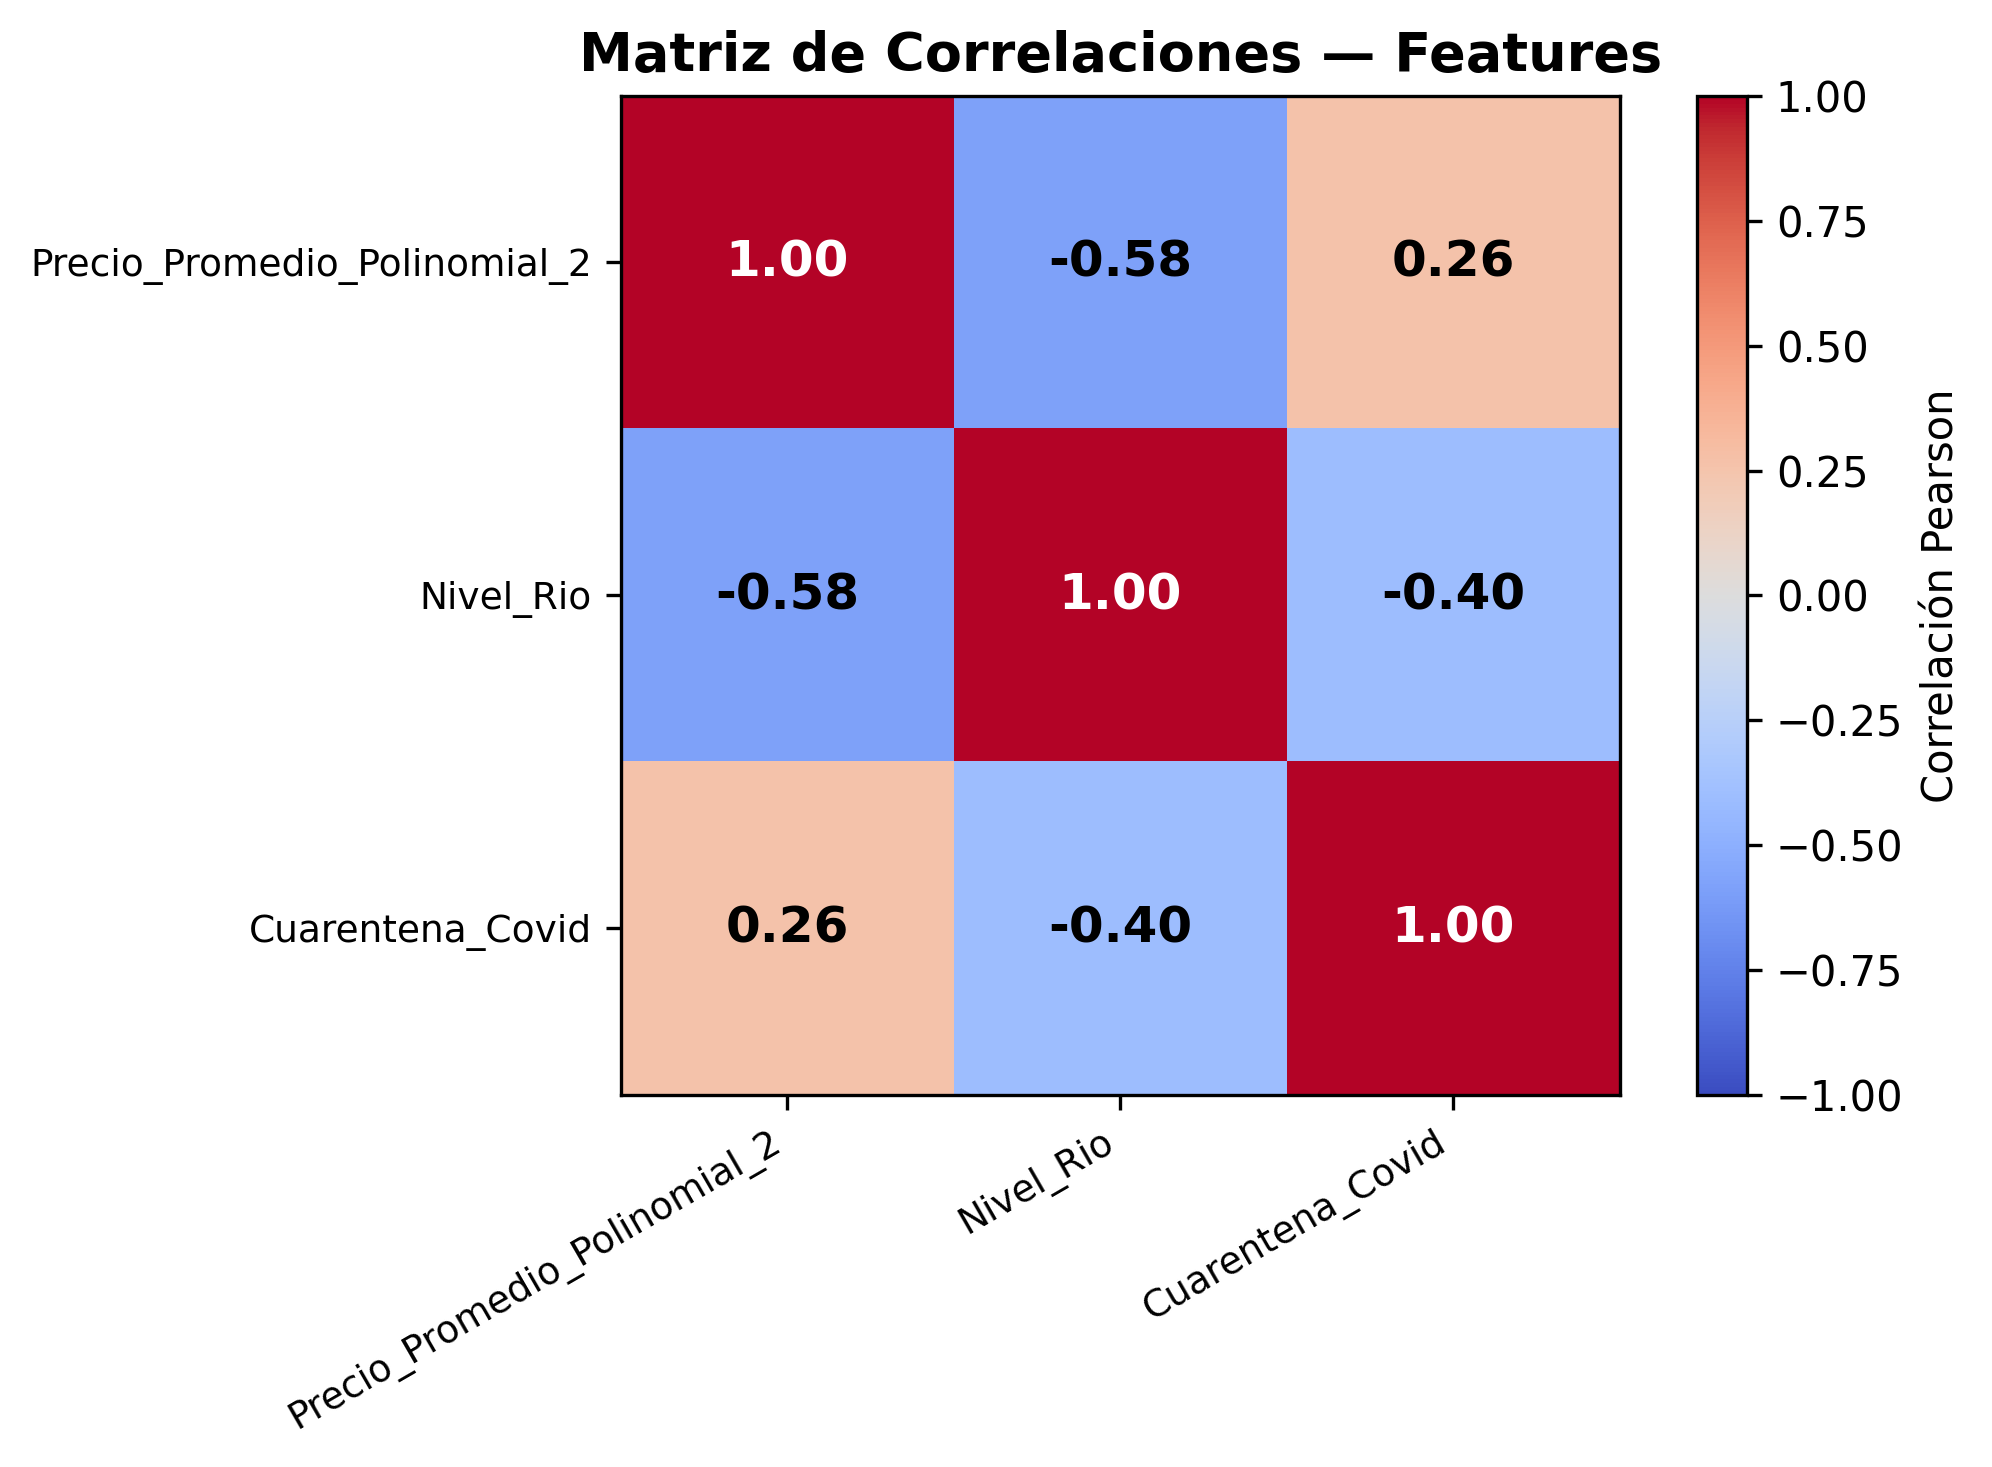
\includegraphics[width=\textwidth]{predicciones/prediccion_ladrillo_lstm/resultados_sin_covid/eda_correlaciones_heatmap.png}
    \caption{Mapa de calor de correlaciones entre las variables de entrada del modelo LSTM para ladrillo.}
    \label{fig:lstm_ladrillo_eda_corr}
\end{figure}

% ------ LADRILLO SIN COVID ------
\clearpage
\subsubsection{Escenario sin Efecto Pandémico}

\paragraph{Hiperparámetros y Arquitectura}

\justify
La búsqueda con Optuna (261 ensayos, 480,9 min) convergió a una arquitectura LSTM \textbf{bidireccional} con una capa de 64 unidades ocultas, lo que permite al modelo procesar la secuencia en ambas direcciones y capturar dependencias pasadas y futuras dentro de la ventana de entrada. Se incorporaron \textit{dropout} de 0,2 y \textit{dropout} recurrente de 0,05 como mecanismos de regularización, junto con el optimizador Adam, tasa de aprendizaje $\text{lr}=0{,}006317$, regularización L2 $\lambda=7{,}35 \times 10^{-6}$, \textit{lookback} de 4 meses y \textit{scheduler} StepLR. La Tabla~\ref{tab:lstm_ladrillo_sc_hiper} detalla estos parámetros.

\begin{table}[htbp]
\centering
\caption{Hiperparámetros óptimos del modelo LSTM para ladrillo --- escenario sin pandemia (Optuna: 261 ensayos).}
\label{tab:lstm_ladrillo_sc_hiper}
\begin{tabular}{ll}
\toprule
\textbf{Hiperparámetro} & \textbf{Valor} \\
\midrule
Capas LSTM          & 1 \\
Unidades ocultas    & 64 \\
Bidireccional       & Sí \\
Dropout             & 0,2 \\
Dropout recurrente  & 0,05 \\
Optimizador         & Adam \\
Tasa de aprendizaje & 0,006317 \\
Regularización L2   & $7{,}35 \times 10^{-6}$ \\
Lookback            & 4 meses \\
Batch size          & 4 \\
Scheduler           & StepLR \\
Parámetros entrenables & 36.993 \\
\bottomrule
\end{tabular}
\end{table}

\paragraph{Curva de Aprendizaje}

\begin{figure}[htbp]
    \centering
    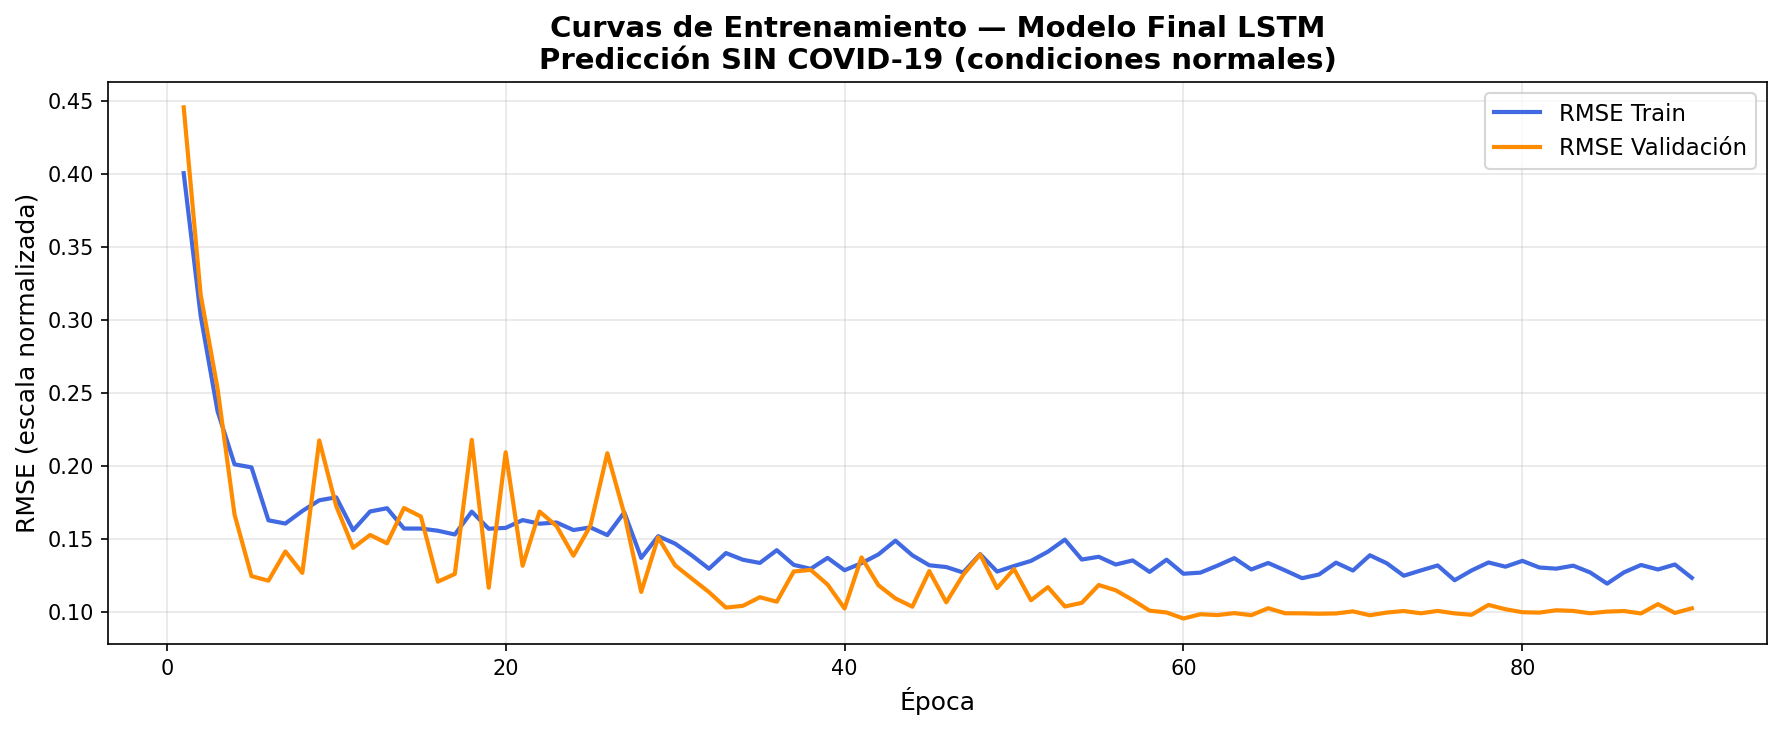
\includegraphics[width=0.85\textwidth]{predicciones/prediccion_ladrillo_lstm/resultados_sin_covid/final_01_curvas_entrenamiento.png}
    \caption{Curva de aprendizaje del modelo LSTM para ladrillo --- escenario sin pandemia.}
    \label{fig:lstm_ladrillo_curva_sc}
\end{figure}

\paragraph{Métricas de Evaluación}

\begin{table}[htbp]
\centering
\caption{Desempeño del modelo LSTM para ladrillo --- escenario sin pandemia: RMSE en train, val y test.}
\label{tab:lstm_ladrillo_sc_metricas}
\begin{tabular}{lrrr}
\toprule
\textbf{Métrica} & \textbf{Train} & \textbf{Val} & \textbf{Test} \\
\midrule
RMSE (Gs.) & 13,76 & 12,53 & 6,32 \\
\bottomrule
\end{tabular}
\end{table}

\justify
El RMSE de prueba de 6,32~Gs.\ representa un error relativo inferior al 2\,\% del rango histórico de la serie (Gs.~428--700), evidenciando una capacidad predictiva excelente. El hecho de que sea incluso menor que el de entrenamiento (13,76~Gs.) indica que el período de prueba presenta menor volatilidad que el período de entrenamiento.

\paragraph{Evaluación sobre el Conjunto de Prueba}

\begin{figure}[htbp]
    \centering
    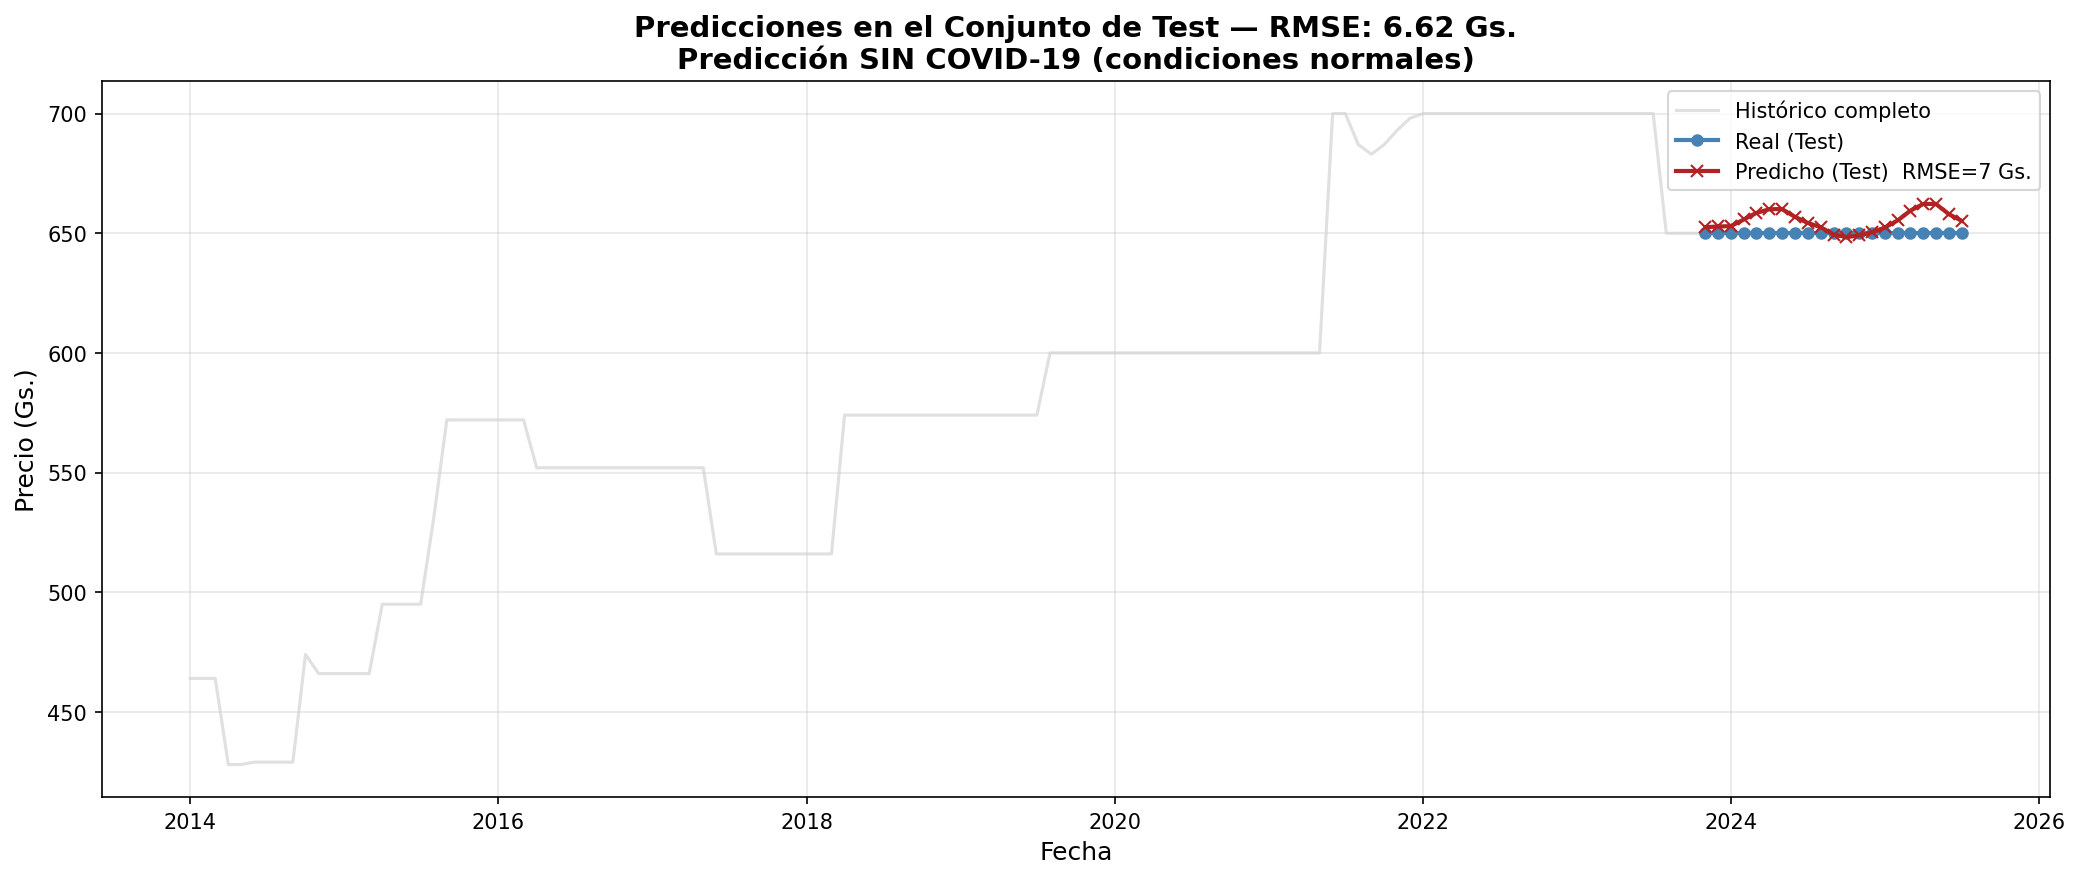
\includegraphics[width=\textwidth]{predicciones/prediccion_ladrillo_lstm/resultados_sin_covid/final_02_prediccion_test_serie.png}
    \caption{Predicción LSTM vs.\ valores reales del precio del ladrillo --- escenario sin pandemia, conjunto de prueba.}
    \label{fig:lstm_ladrillo_test_sc}
\end{figure}

\begin{figure}[htbp]
    \centering
    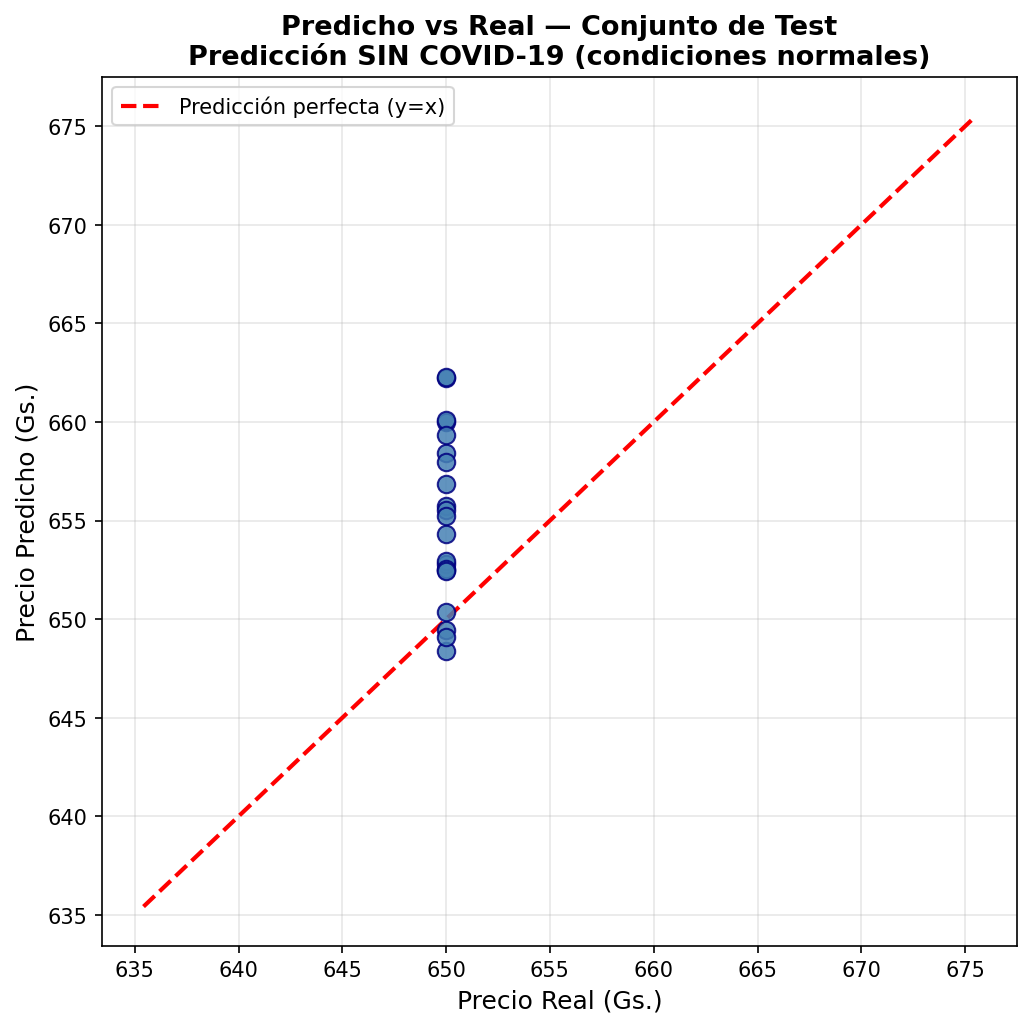
\includegraphics[width=0.7\textwidth]{predicciones/prediccion_ladrillo_lstm/resultados_sin_covid/final_03_scatter_test.png}
    \caption{Diagrama de dispersión: precio predicho vs.\ real del ladrillo --- escenario sin pandemia.}
    \label{fig:lstm_ladrillo_scatter_sc}
\end{figure}

\begin{figure}[htbp]
    \centering
    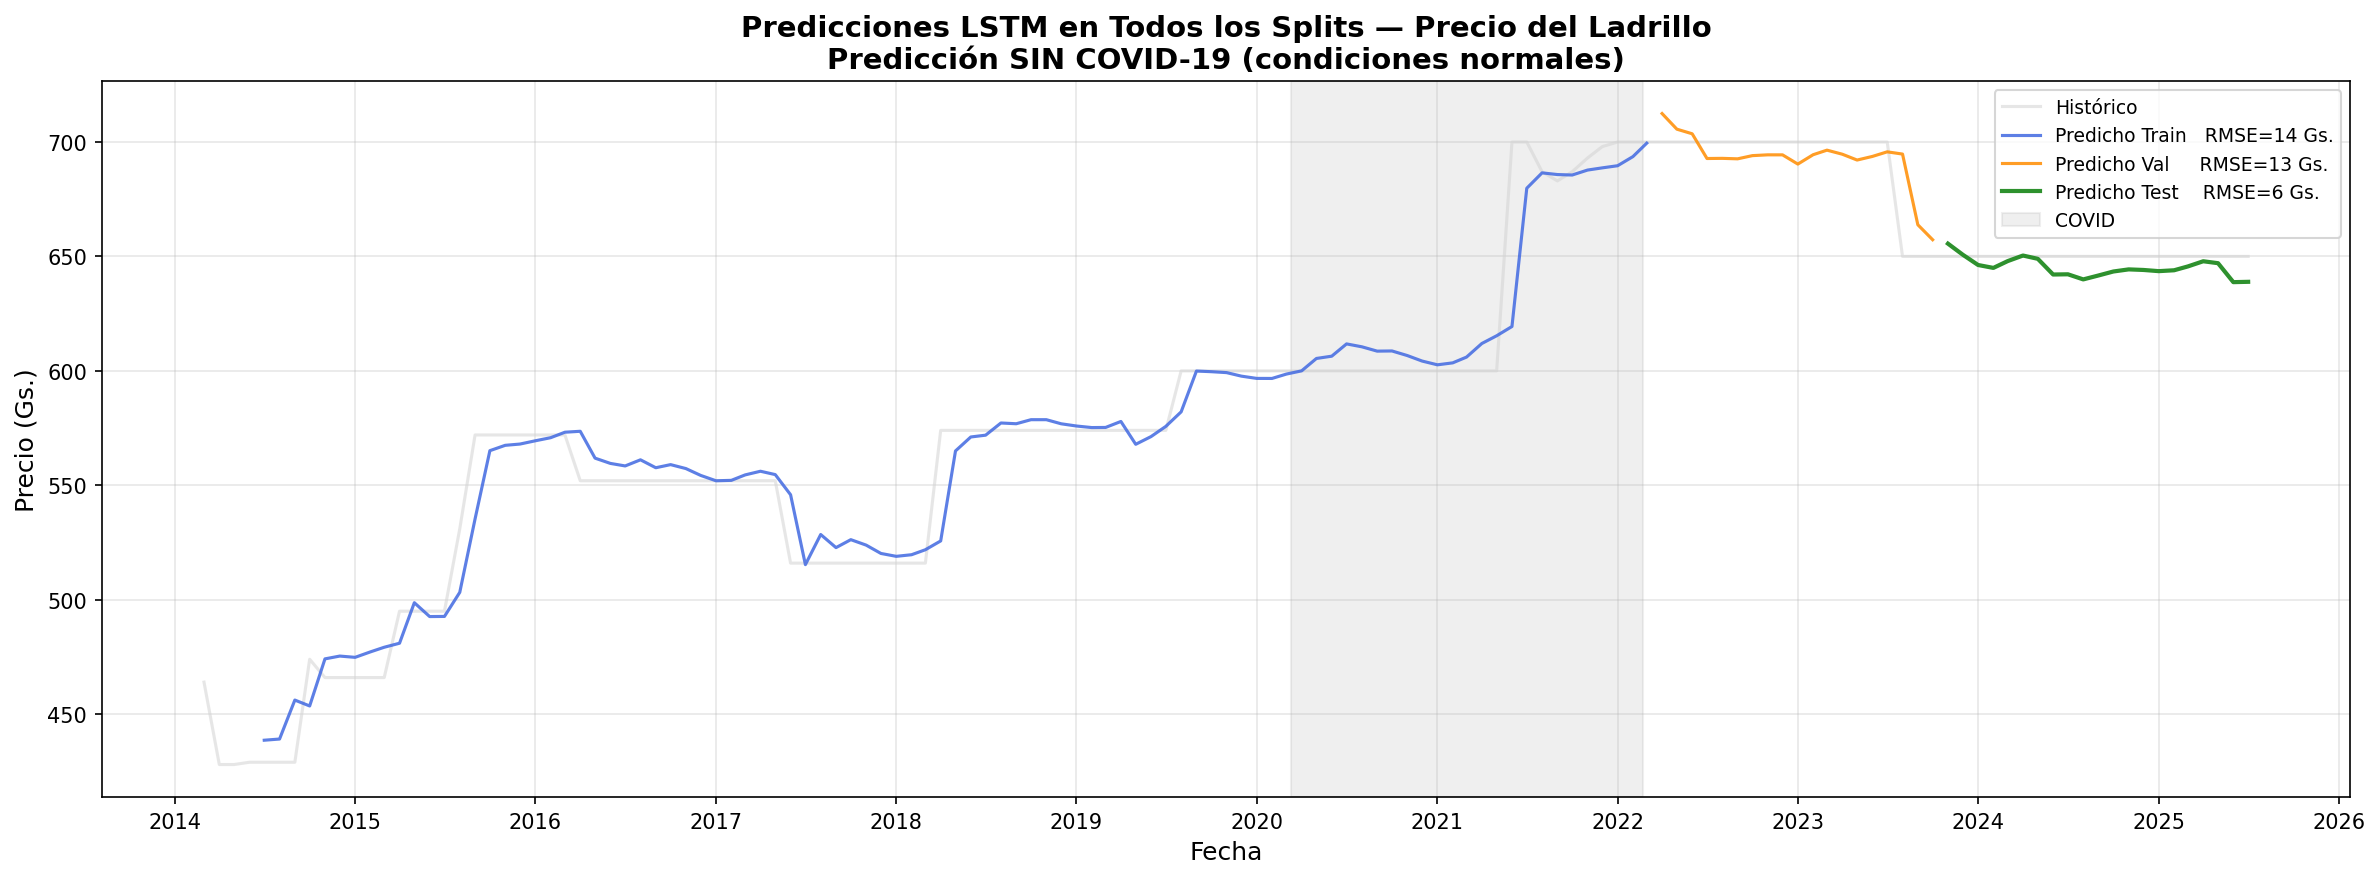
\includegraphics[width=\textwidth]{predicciones/prediccion_ladrillo_lstm/resultados_sin_covid/final_05_todos_splits.png}
    \caption{Ajuste del modelo LSTM del ladrillo sobre las tres particiones --- escenario sin pandemia.}
    \label{fig:lstm_ladrillo_splits_sc}
\end{figure}

\clearpage
\paragraph{Análisis de Residuos}

\begin{figure}[htbp]
    \centering
    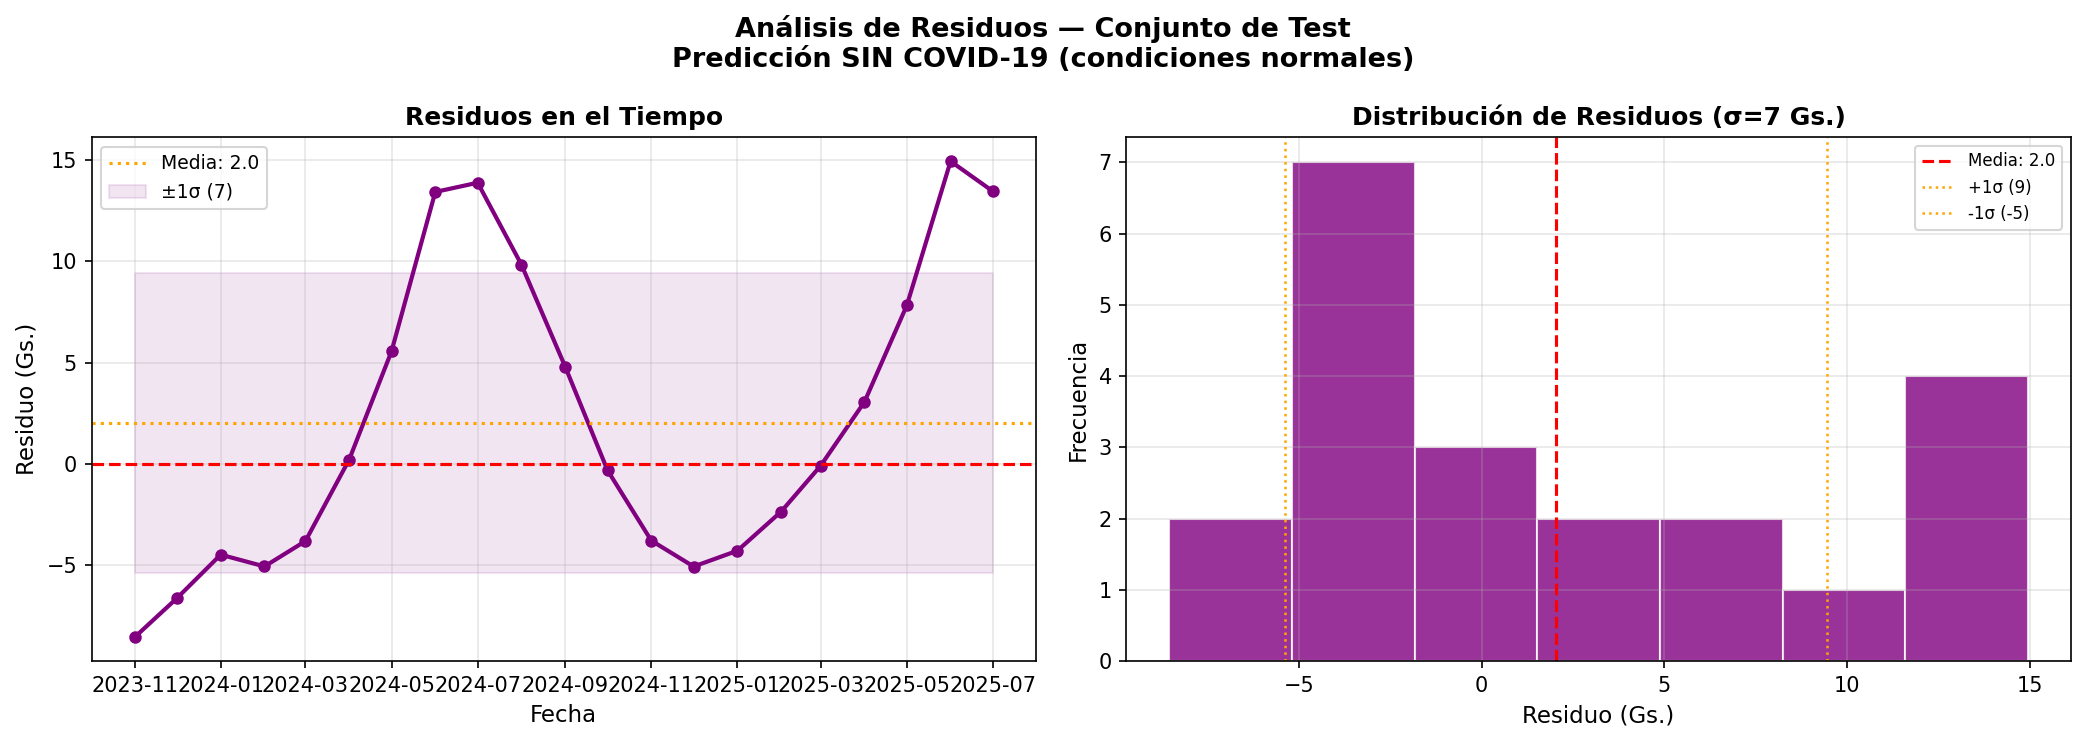
\includegraphics[width=\textwidth]{predicciones/prediccion_ladrillo_lstm/resultados_sin_covid/final_04_residuos.png}
    \caption{Residuos del modelo LSTM para ladrillo sobre el conjunto de prueba --- escenario sin pandemia.}
    \label{fig:lstm_ladrillo_res_sc}
\end{figure}

\begin{figure}[htbp]
    \centering
    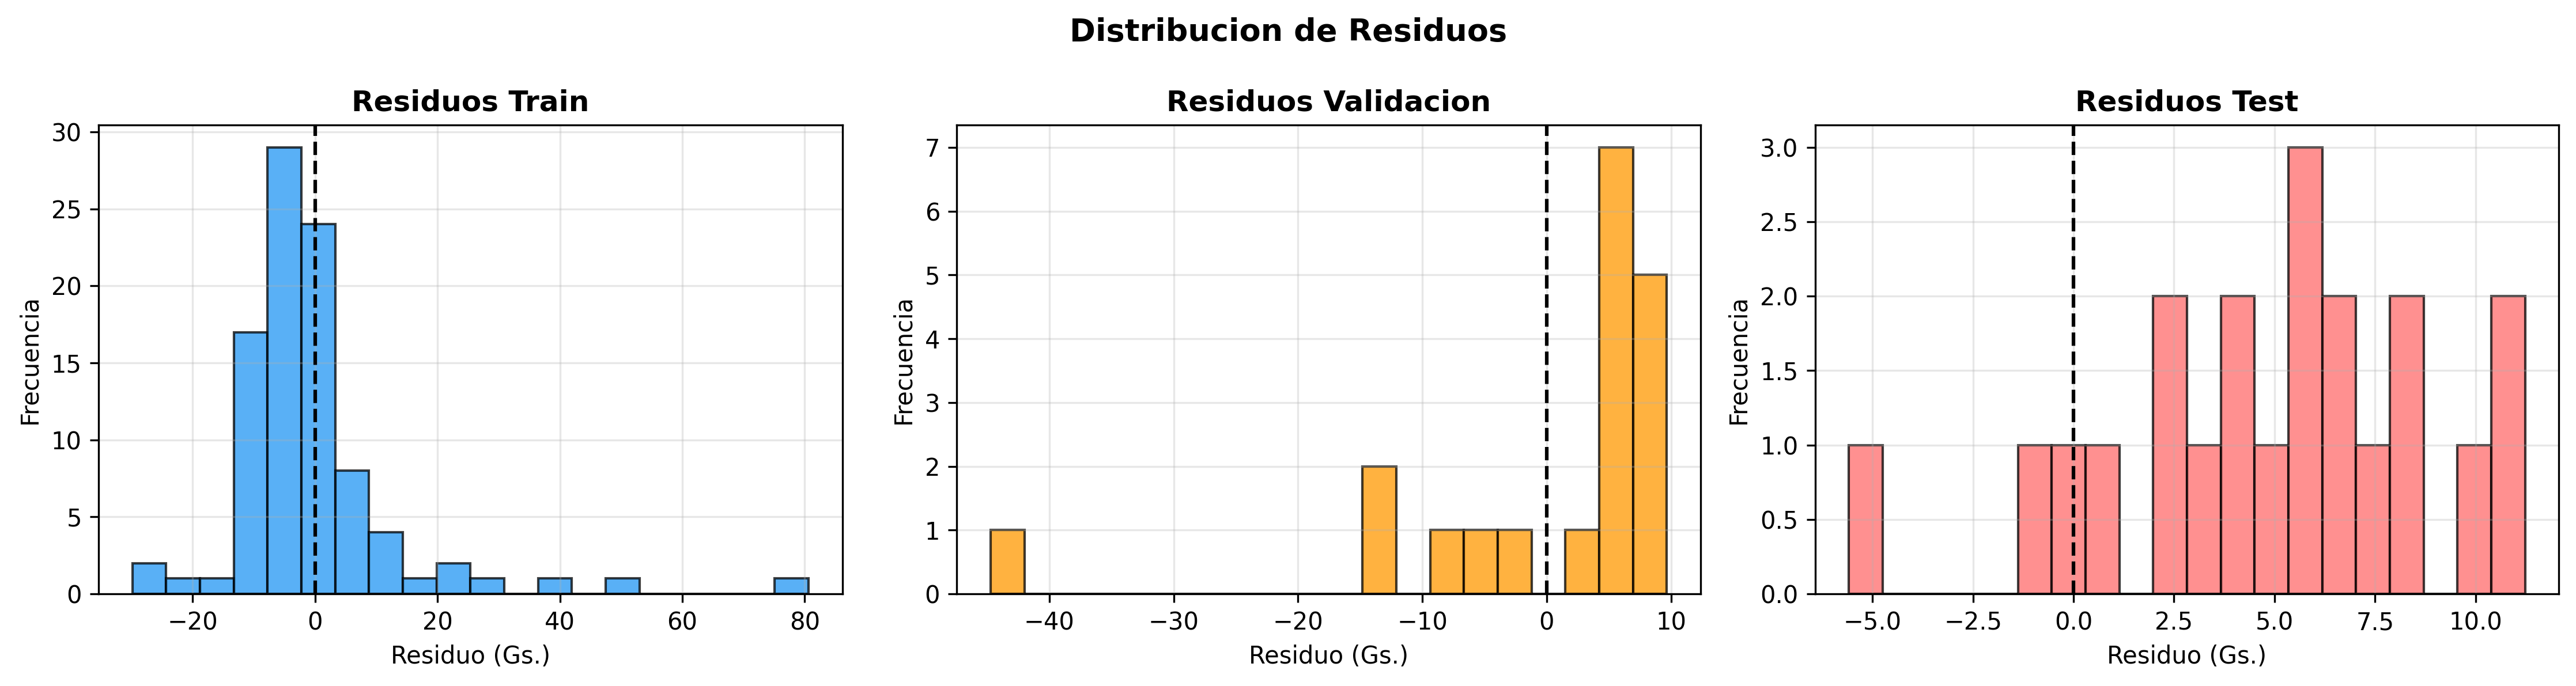
\includegraphics[width=0.75\textwidth]{predicciones/prediccion_ladrillo_lstm/resultados_sin_covid/residuos_histograma.png}
    \caption{Histograma de residuos del modelo LSTM para ladrillo --- escenario sin pandemia.}
    \label{fig:lstm_ladrillo_reshist_sc}
\end{figure}

\begin{figure}[htbp]
    \centering
    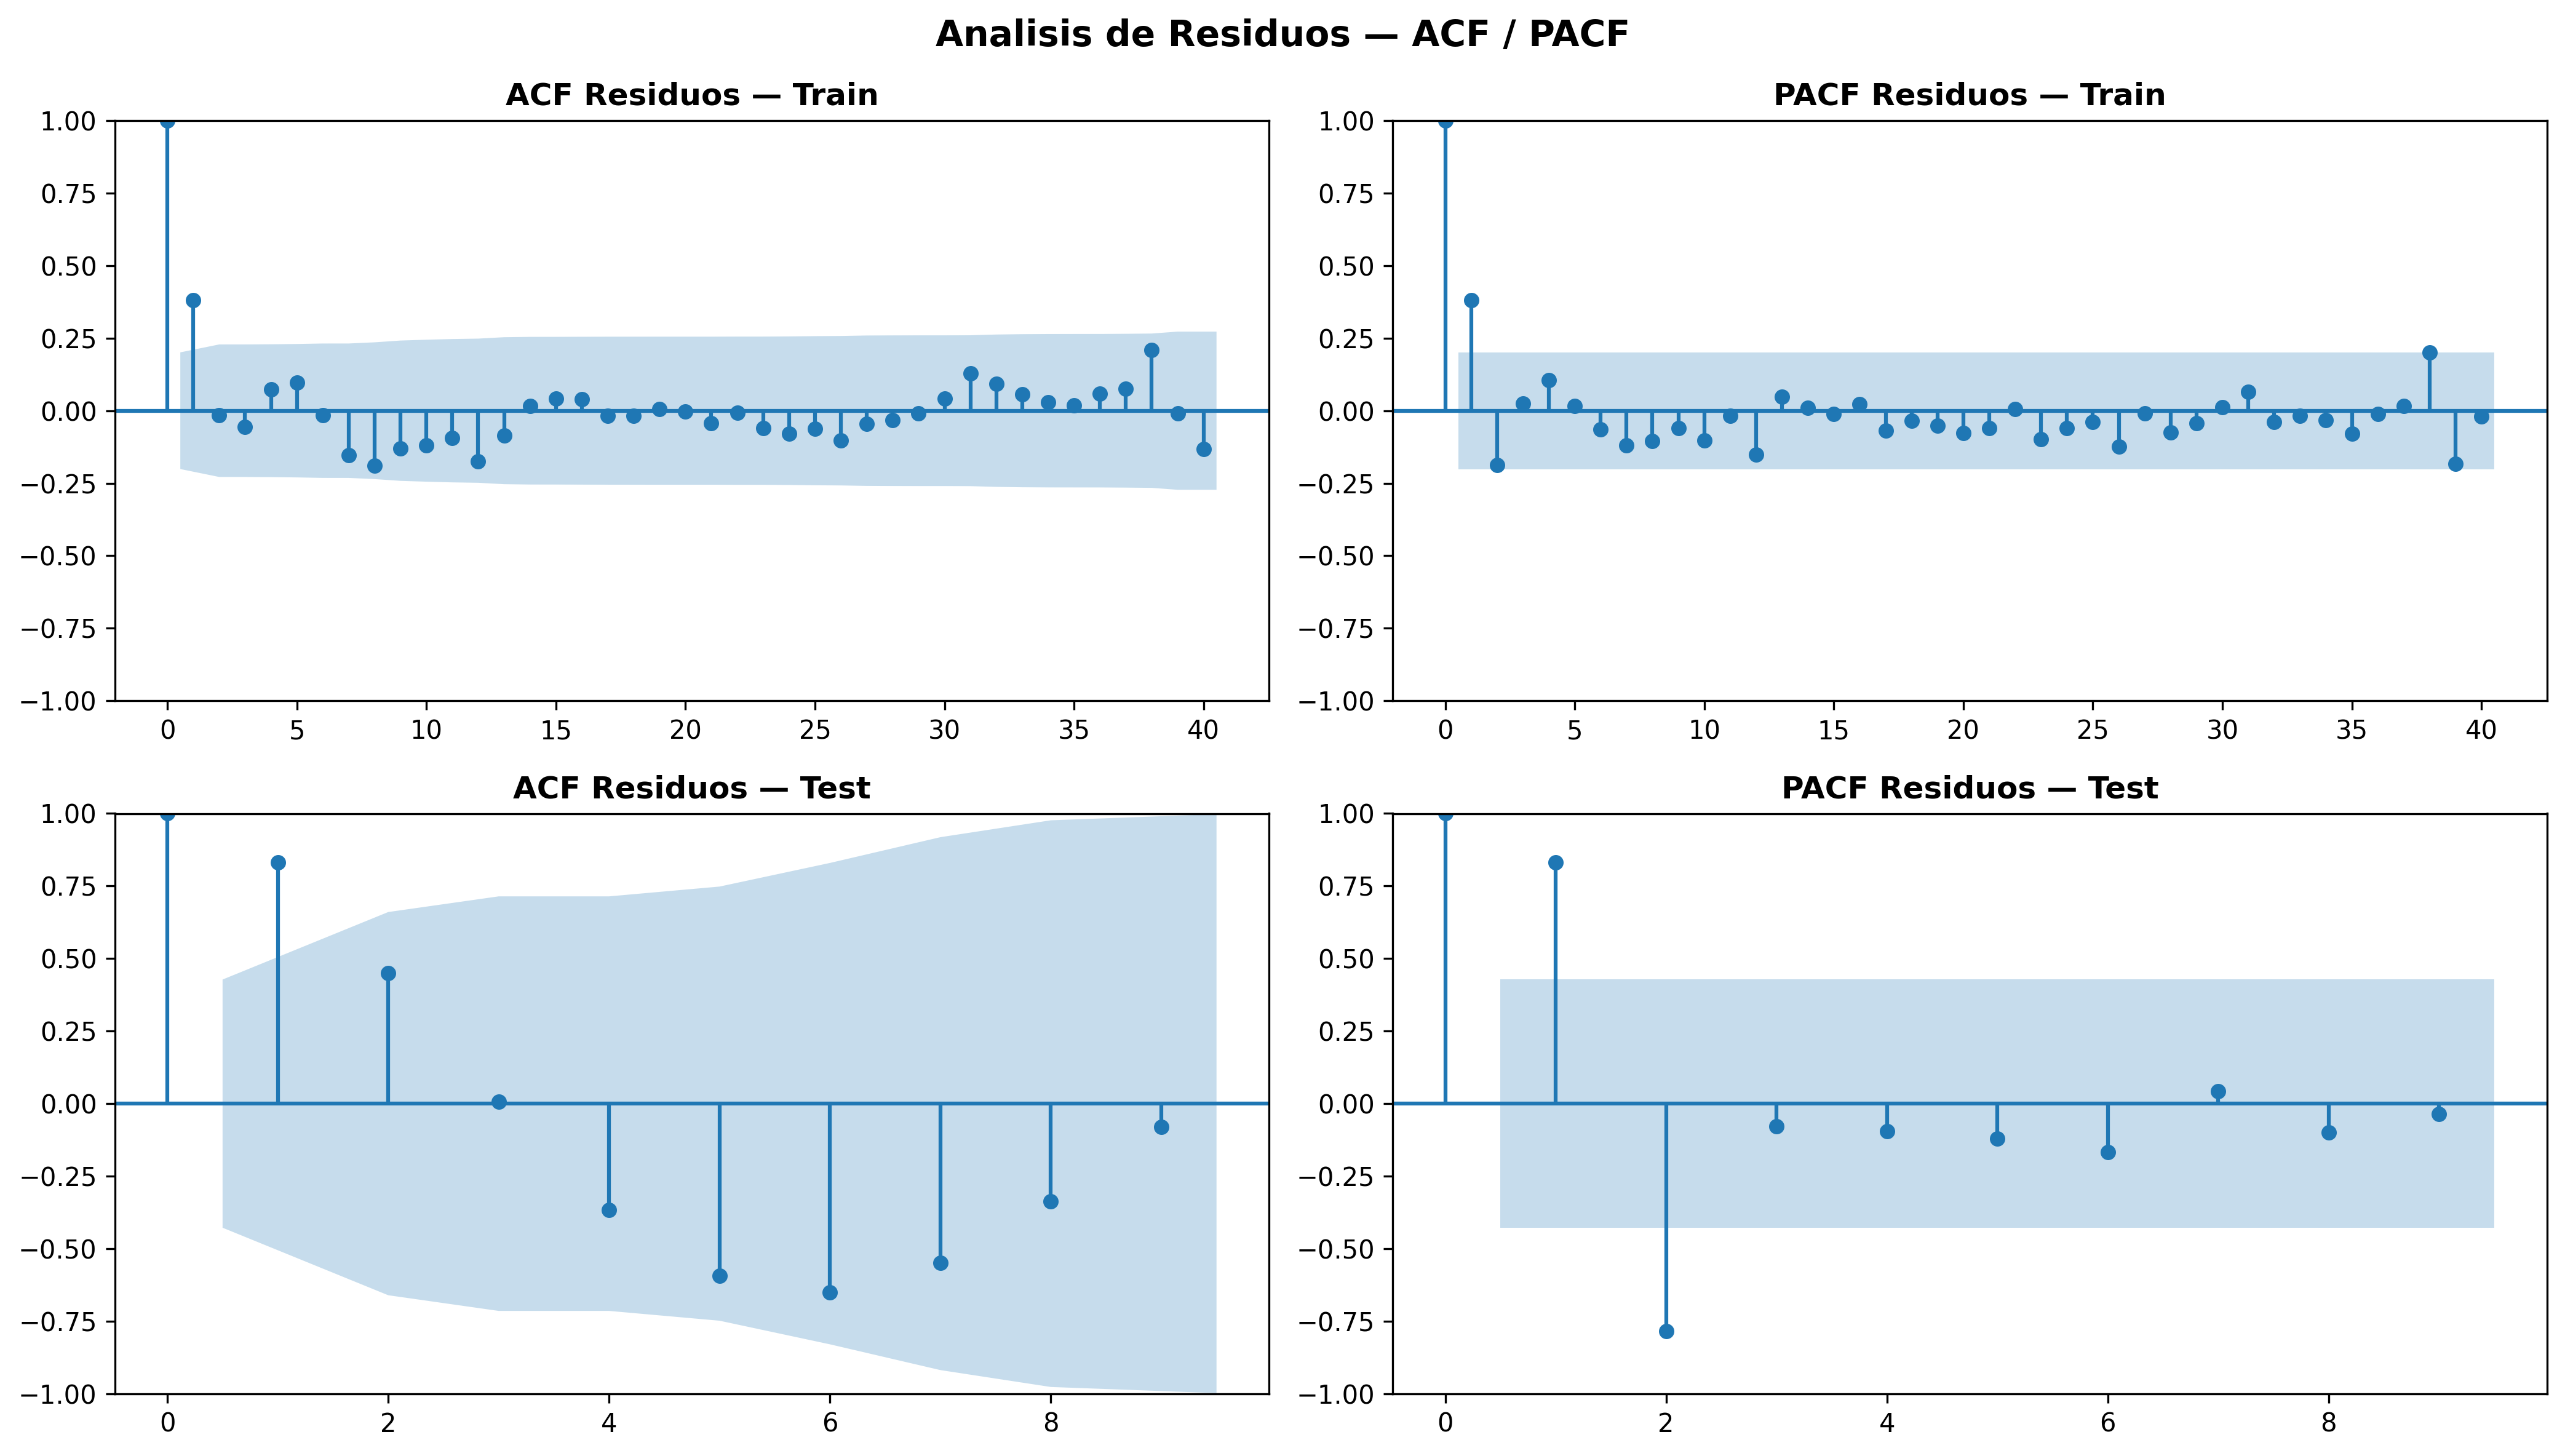
\includegraphics[width=\textwidth]{predicciones/prediccion_ladrillo_lstm/resultados_sin_covid/residuos_acf_pacf.png}
    \caption{ACF y PACF de los residuos del modelo LSTM para ladrillo --- escenario sin pandemia.}
    \label{fig:lstm_ladrillo_resacf_sc}
\end{figure}

\justify
El test de Ljung-Box sobre los residuos del conjunto de prueba muestra un $p$-valor de 0,237 a 10 rezagos (no rechaza $H_0$) y un $p$-valor de $1{,}05 \times 10^{-5}$ a 20 rezagos (rechaza $H_0$). Esto indica que los residuos se comportan como ruido blanco en el corto plazo, aunque existen patrones de dependencia en rezagos más distantes, posiblemente asociados a estacionalidad no capturada completamente.

\clearpage
\paragraph{Pronóstico a 24 Meses}

\begin{figure}[htbp]
    \centering
    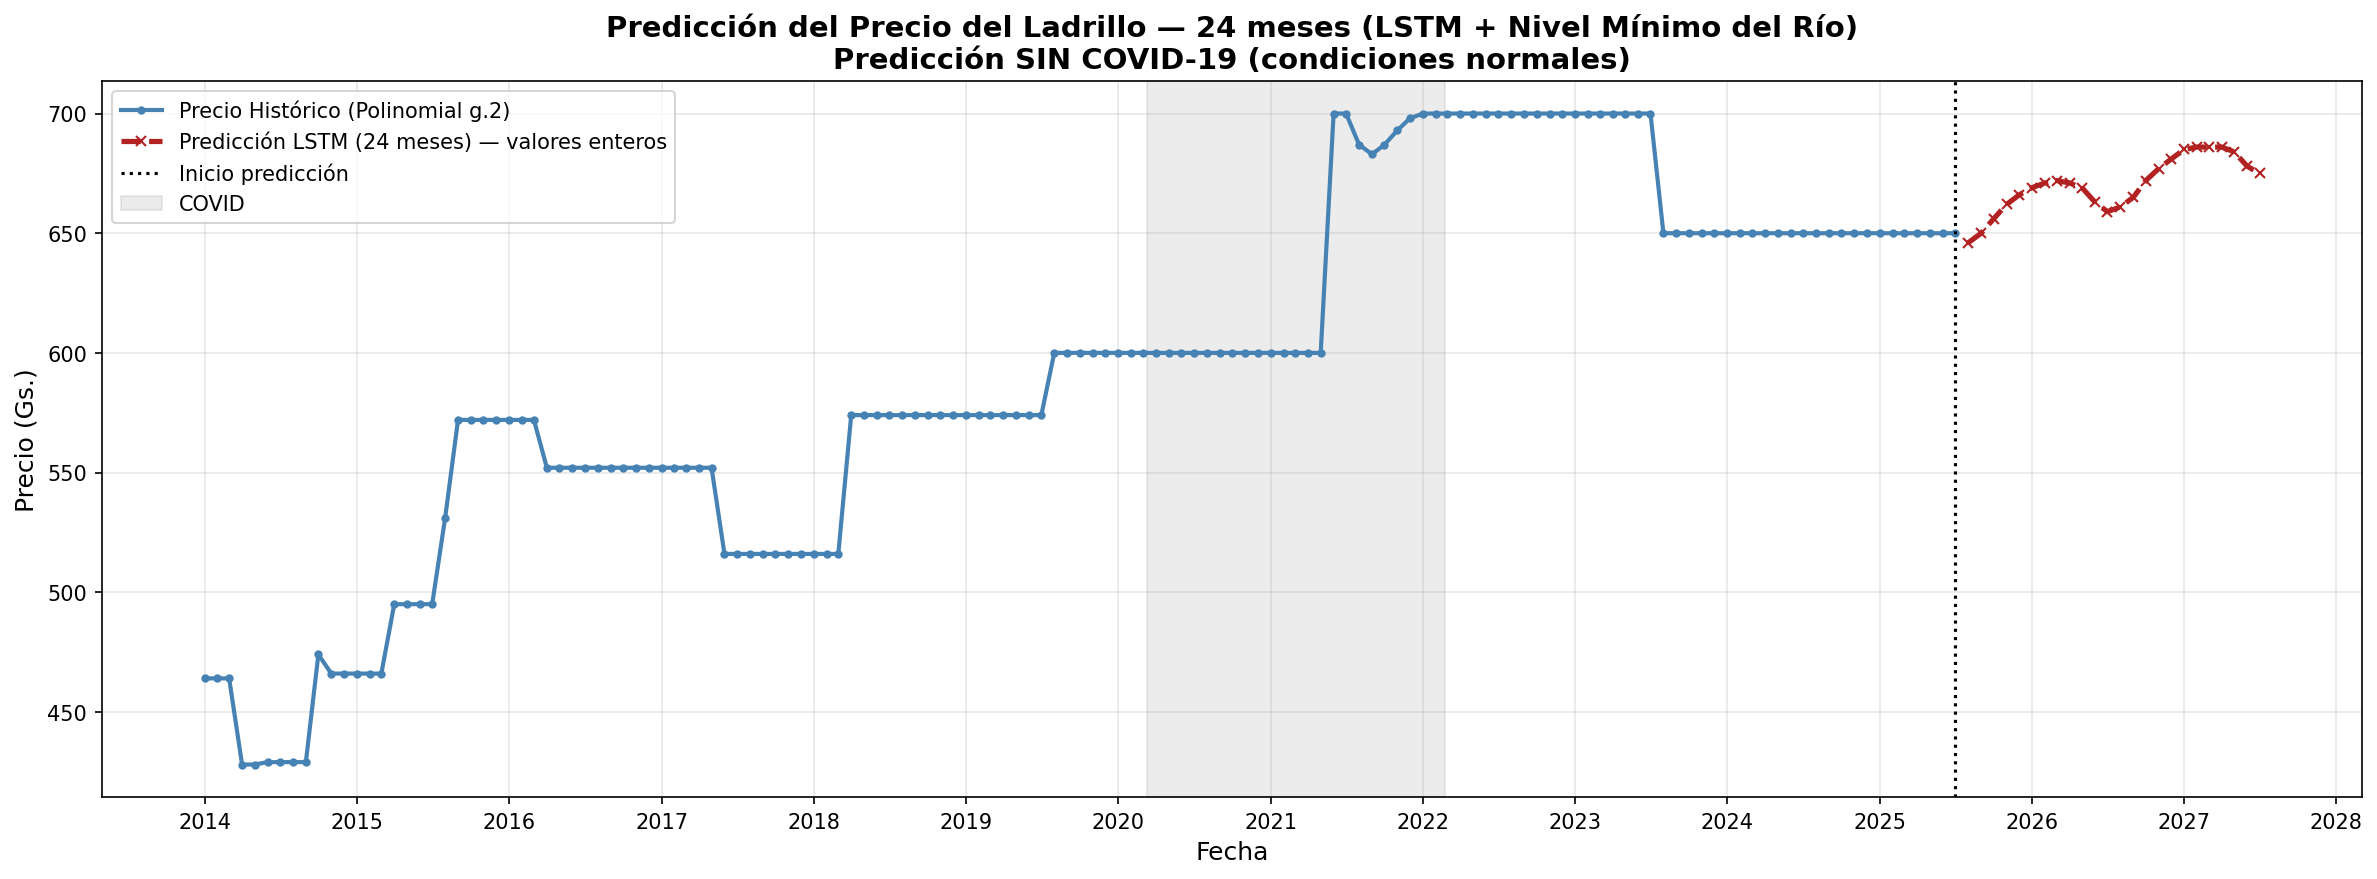
\includegraphics[width=\textwidth]{predicciones/prediccion_ladrillo_lstm/resultados_sin_covid/final_06_prediccion_futura_completa.png}
    \caption{Pronóstico LSTM a 24 meses del precio del ladrillo --- escenario sin pandemia, con IC al 95\,\%.}
    \label{fig:lstm_ladrillo_pred_sin_covid}
\end{figure}

\begin{figure}[htbp]
    \centering
    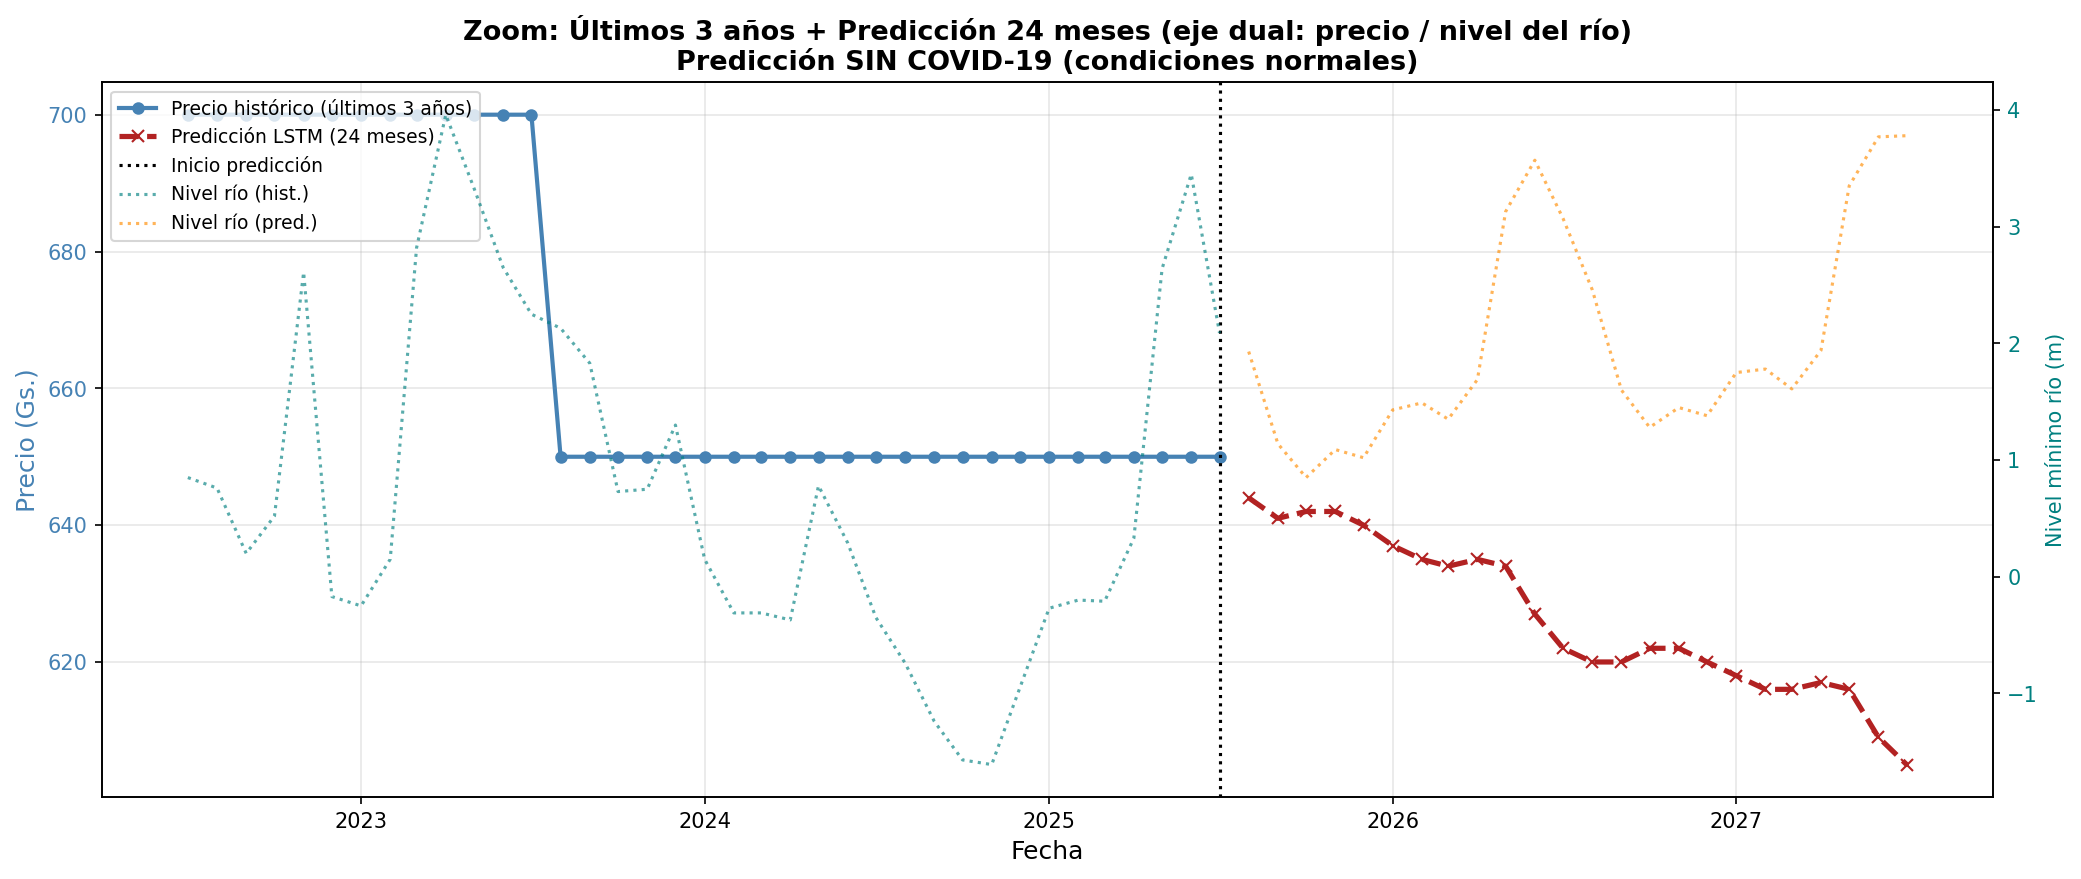
\includegraphics[width=\textwidth]{predicciones/prediccion_ladrillo_lstm/resultados_sin_covid/final_07_prediccion_zoom_dual.png}
    \caption{Detalle de la transición histórico--pronóstico LSTM del ladrillo --- escenario sin pandemia.}
    \label{fig:lstm_ladrillo_zoom_sin_covid}
\end{figure}

\begin{figure}[htbp]
    \centering
    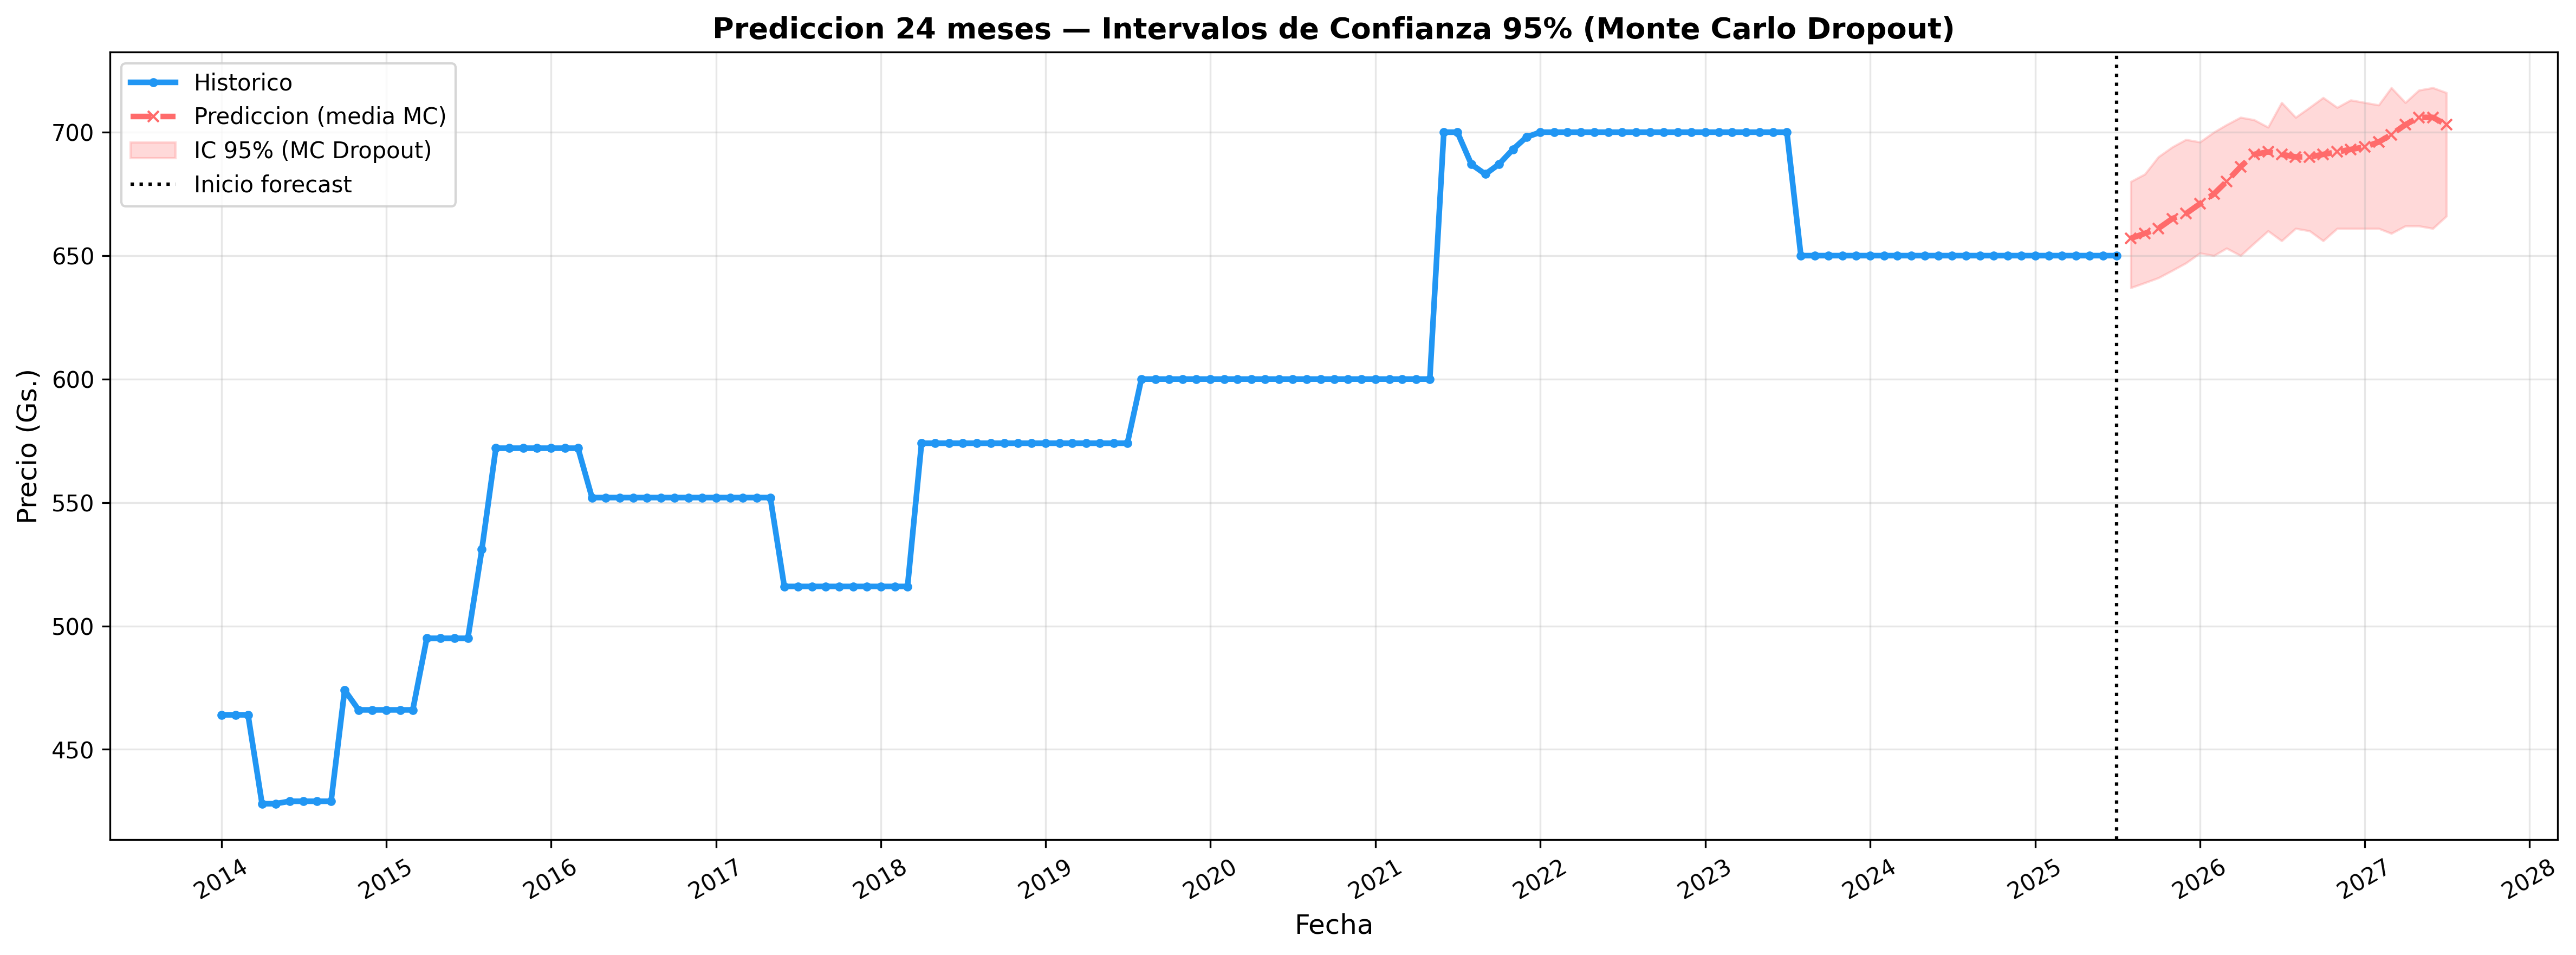
\includegraphics[width=\textwidth]{predicciones/prediccion_ladrillo_lstm/resultados_sin_covid/forecast_ic_monte_carlo.png}
    \caption{IC Monte Carlo Dropout del pronóstico LSTM para ladrillo --- escenario sin pandemia.}
    \label{fig:lstm_ladrillo_ic_mc_sin_covid}
\end{figure}

\justify
Bajo el escenario sin pandemia, el rango de precios predicho se sitúa entre Gs.~605 y Gs.~644 a lo largo del horizonte de 24 meses, un rango estrecho que refleja la estabilidad relativa del precio del ladrillo en condiciones normales de mercado.

% ------ LADRILLO CON COVID ------
\clearpage
\subsubsection{Escenario con Efecto Pandémico}

\paragraph{Hiperparámetros y Arquitectura}

\justify
Para el escenario con efecto pandémico, la búsqueda con Optuna convergió a una arquitectura diferente: una capa LSTM \textbf{unidireccional} con 64 unidades ocultas, sin \textit{dropout} ni planificador de tasa de aprendizaje. El optimizador fue Adam con $\text{lr}=0{,}001$, regularización L2 $\lambda=10^{-5}$, \textit{lookback} de 6 meses y \textit{batch size} de 4. La Tabla~\ref{tab:lstm_ladrillo_cc_hiper} detalla estos parámetros.

\begin{table}[htbp]
\centering
\caption{Hiperparámetros del modelo LSTM para ladrillo --- escenario con pandemia.}
\label{tab:lstm_ladrillo_cc_hiper}
\begin{tabular}{ll}
\toprule
\textbf{Hiperparámetro} & \textbf{Valor} \\
\midrule
Capas LSTM          & 1 \\
Unidades ocultas    & 64 \\
Bidireccional       & No \\
Dropout             & 0,0 \\
Dropout recurrente  & 0,0 \\
Optimizador         & Adam \\
Tasa de aprendizaje & 0,001 \\
Regularización L2   & $10^{-5}$ \\
Lookback            & 6 meses \\
Batch size          & 4 \\
Scheduler           & Ninguno \\
Parámetros entrenables & 18.497 \\
\bottomrule
\end{tabular}
\end{table}

\paragraph{Curva de Aprendizaje}

\begin{figure}[htbp]
    \centering
    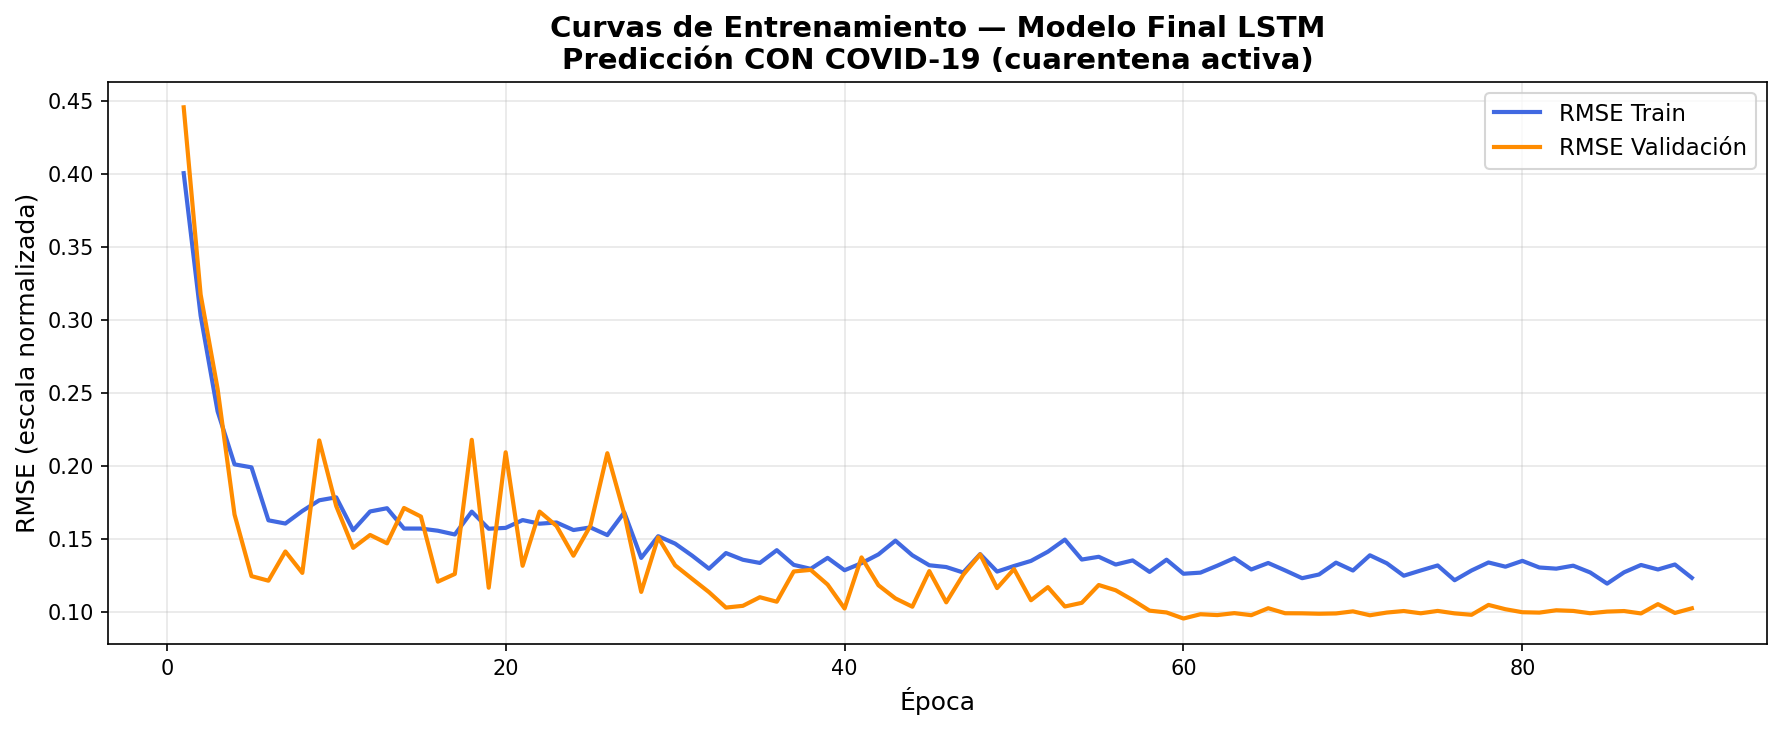
\includegraphics[width=0.85\textwidth]{predicciones/prediccion_ladrillo_lstm/resultados_con_covid/final_01_curvas_entrenamiento.png}
    \caption{Curva de aprendizaje del modelo LSTM para ladrillo --- escenario con pandemia.}
    \label{fig:lstm_ladrillo_curva_cc}
\end{figure}

\paragraph{Métricas de Evaluación}

\begin{table}[htbp]
\centering
\caption{Desempeño del modelo LSTM para ladrillo --- escenario con pandemia: RMSE en train, val y test.}
\label{tab:lstm_ladrillo_cc_metricas}
\begin{tabular}{lrrr}
\toprule
\textbf{Métrica} & \textbf{Train} & \textbf{Val} & \textbf{Test} \\
\midrule
RMSE (Gs.) & 18,59 & 17,54 & 9,13 \\
\bottomrule
\end{tabular}
\end{table}

\justify
El RMSE de prueba de 9,13~Gs.\ es superior al obtenido en el escenario sin pandemia (6,32~Gs.), lo que refleja que la arquitectura unidireccional más simple ---con el efecto pandémico incluido en el entrenamiento--- no logra el mismo nivel de ajuste que el modelo bidireccional optimizado para el escenario sin pandemia. No obstante, representa un error relativo inferior al 3\,\% del rango histórico de la serie, que sigue siendo aceptable para la predicción de precios de materiales de construcción.

\paragraph{Evaluación sobre el Conjunto de Prueba}

\begin{figure}[htbp]
    \centering
    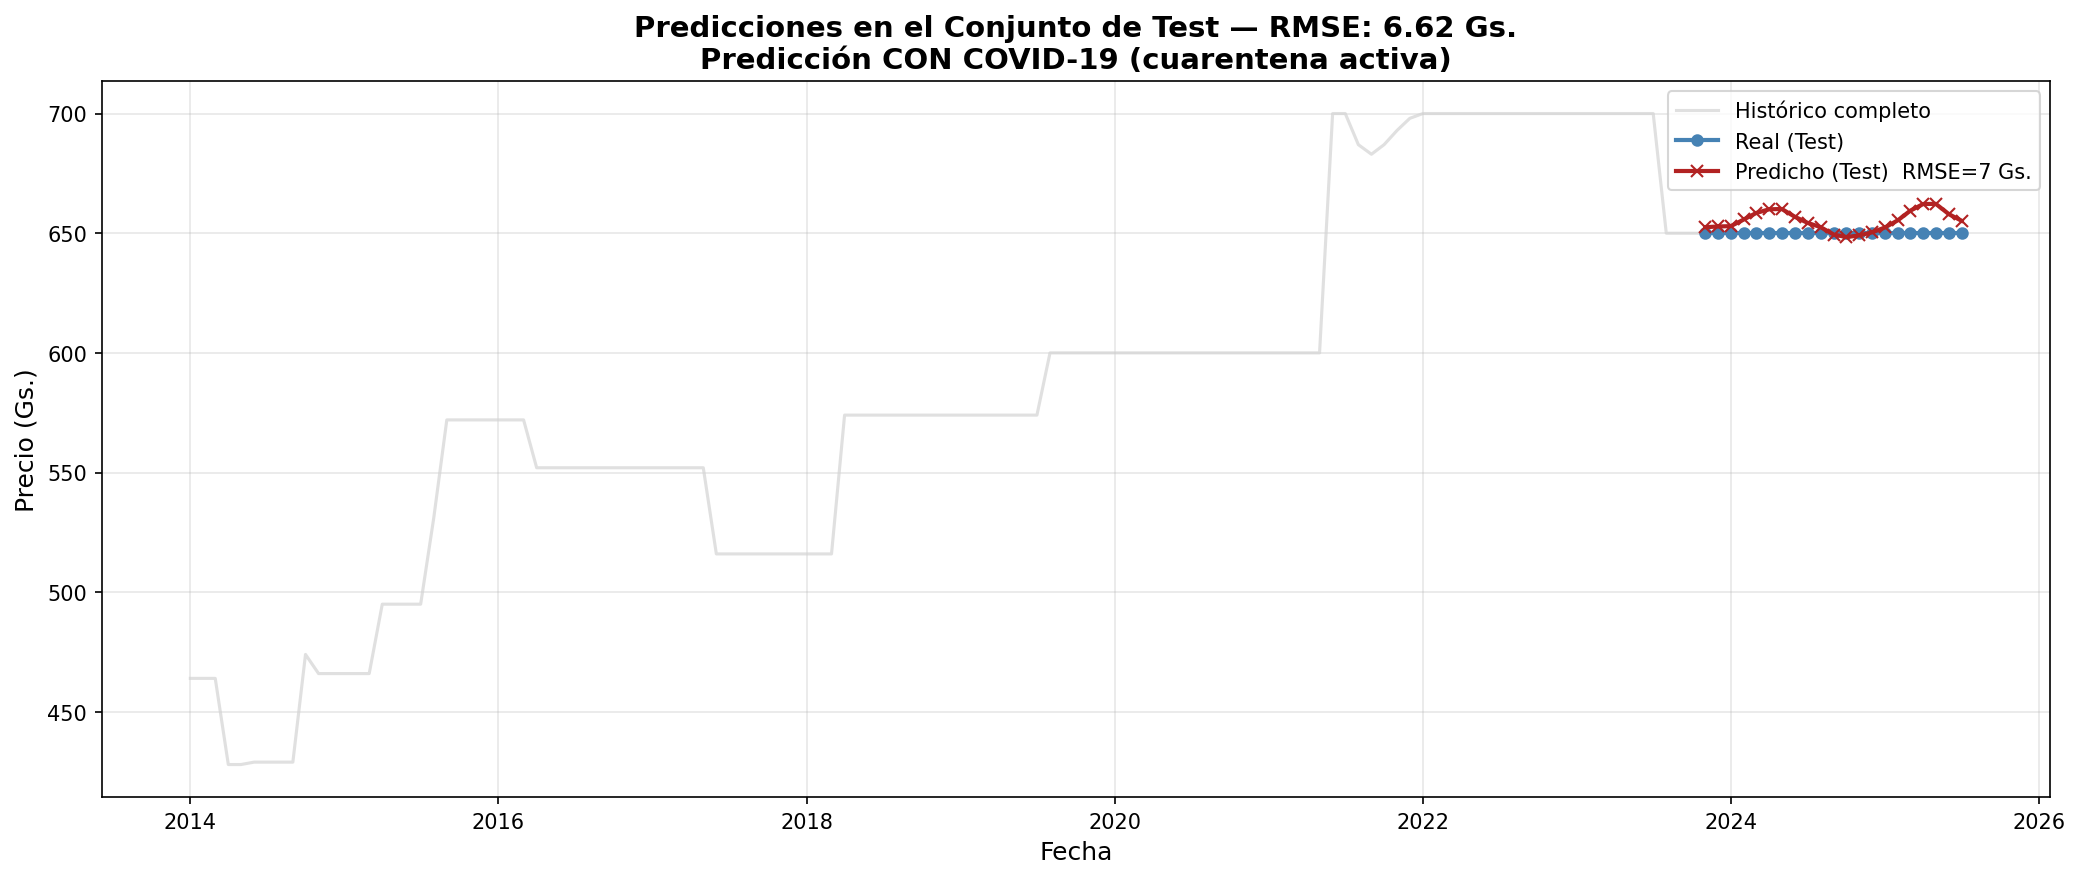
\includegraphics[width=\textwidth]{predicciones/prediccion_ladrillo_lstm/resultados_con_covid/final_02_prediccion_test_serie.png}
    \caption{Predicción LSTM vs.\ valores reales del precio del ladrillo --- escenario con pandemia, conjunto de prueba.}
    \label{fig:lstm_ladrillo_test_cc}
\end{figure}

\begin{figure}[htbp]
    \centering
    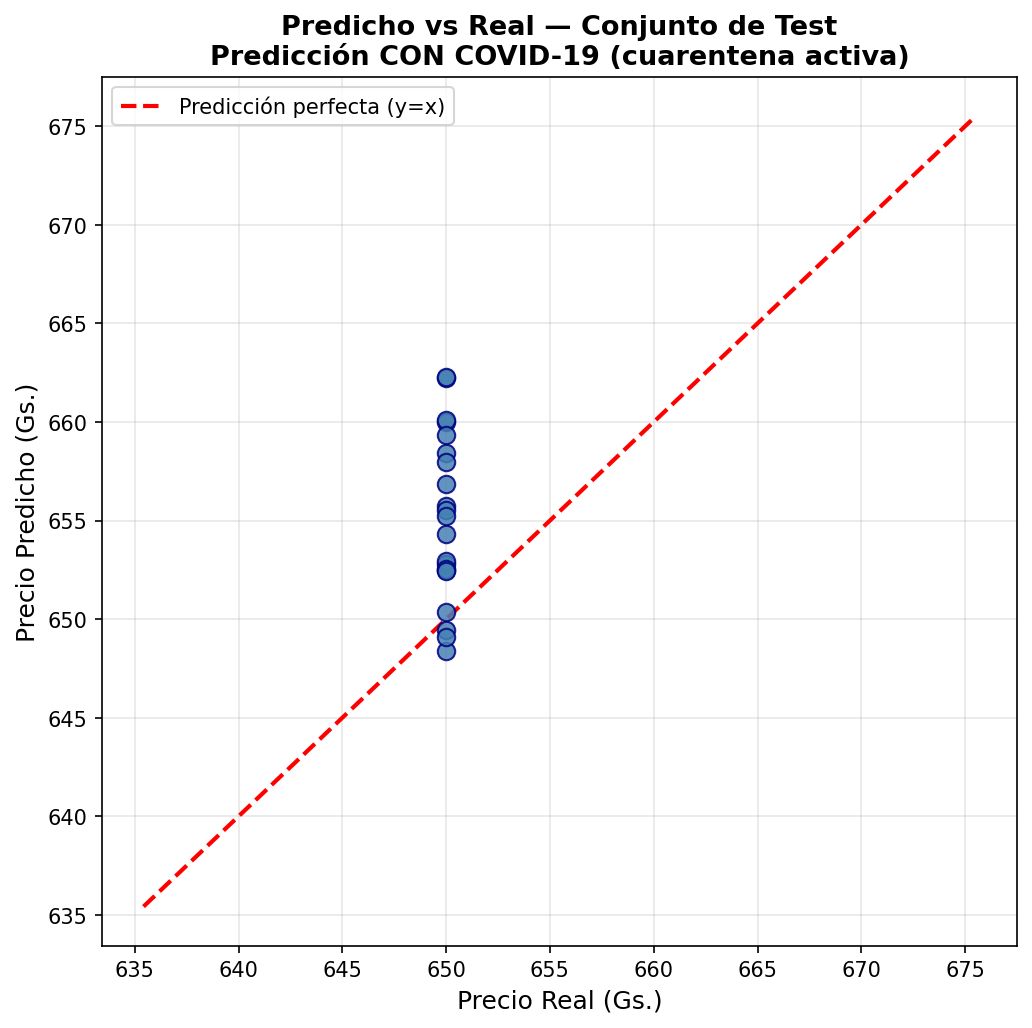
\includegraphics[width=0.7\textwidth]{predicciones/prediccion_ladrillo_lstm/resultados_con_covid/final_03_scatter_test.png}
    \caption{Diagrama de dispersión: precio predicho vs.\ real del ladrillo --- escenario con pandemia.}
    \label{fig:lstm_ladrillo_scatter_cc}
\end{figure}

\begin{figure}[htbp]
    \centering
    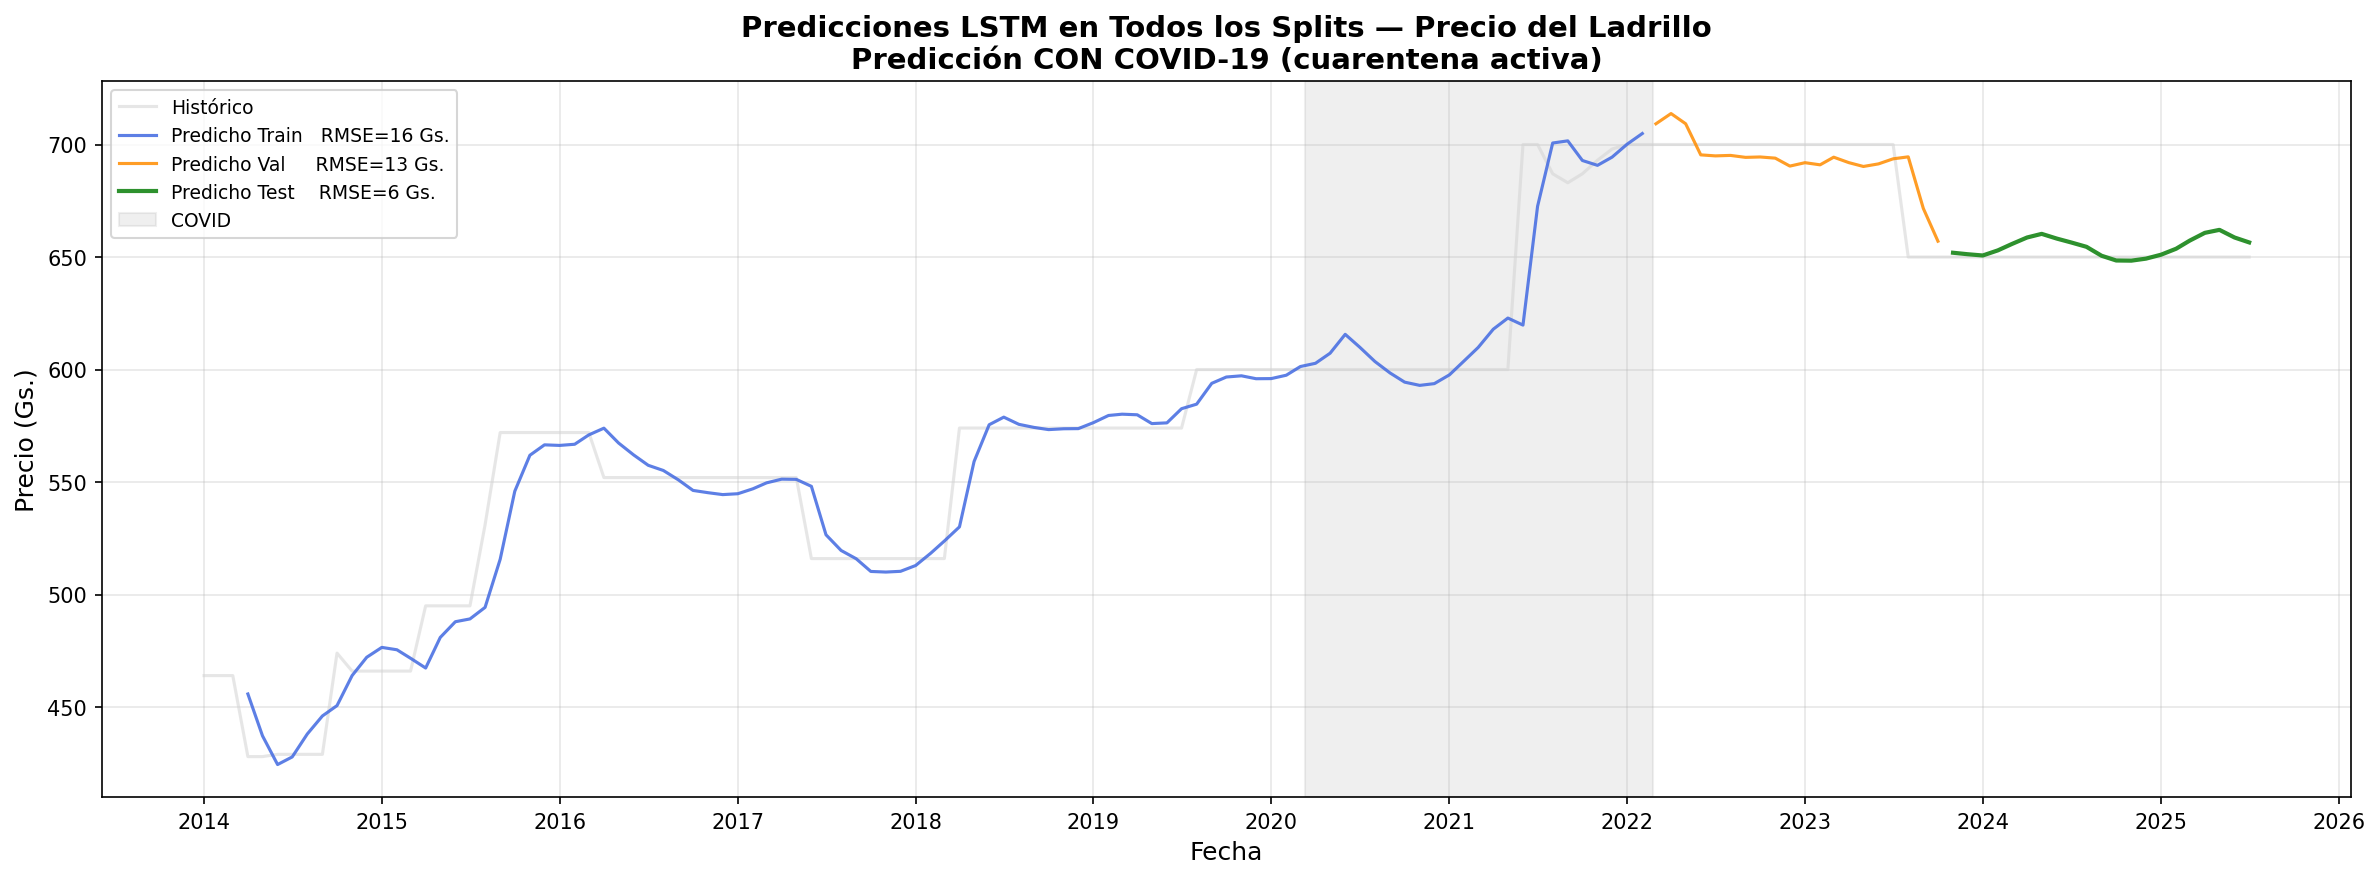
\includegraphics[width=\textwidth]{predicciones/prediccion_ladrillo_lstm/resultados_con_covid/final_05_todos_splits.png}
    \caption{Ajuste del modelo LSTM del ladrillo sobre las tres particiones --- escenario con pandemia.}
    \label{fig:lstm_ladrillo_splits_cc}
\end{figure}

\clearpage
\paragraph{Análisis de Residuos}

\begin{figure}[htbp]
    \centering
    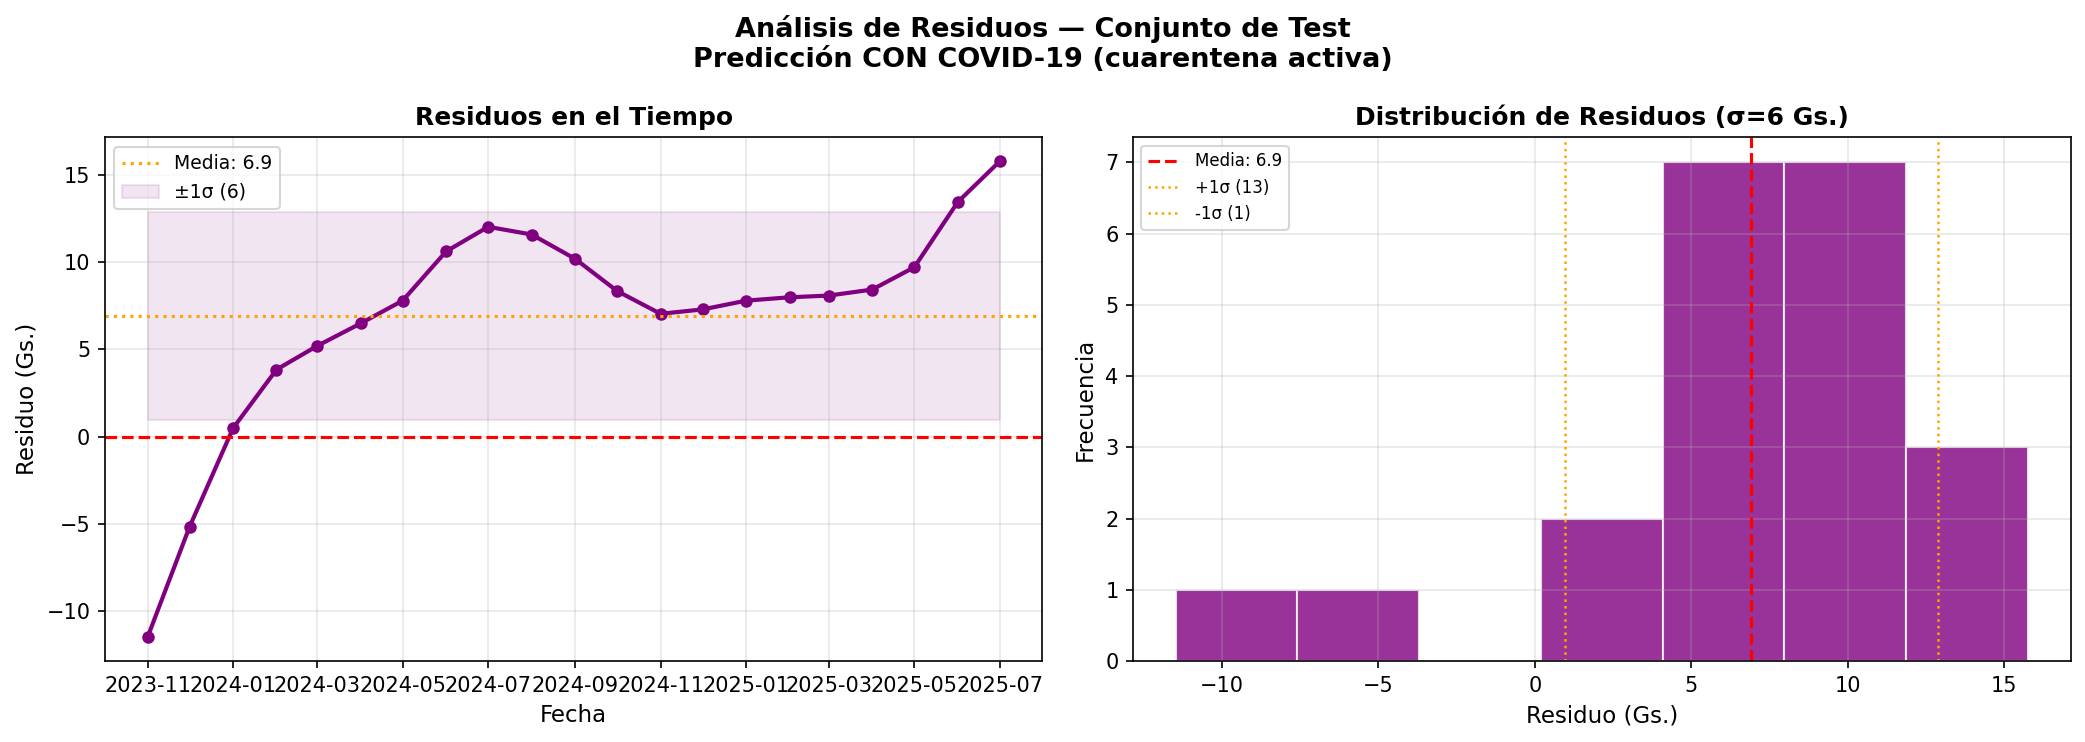
\includegraphics[width=\textwidth]{predicciones/prediccion_ladrillo_lstm/resultados_con_covid/final_04_residuos.png}
    \caption{Residuos del modelo LSTM para ladrillo sobre el conjunto de prueba --- escenario con pandemia.}
    \label{fig:lstm_ladrillo_res_cc}
\end{figure}

\begin{figure}[htbp]
    \centering
    \includegraphics[width=0.75\textwidth]{predicciones/prediccion_ladrillo_lstm/resultados_con_covid/residuos_histograma.png}
    \caption{Histograma de residuos del modelo LSTM para ladrillo --- escenario con pandemia.}
    \label{fig:lstm_ladrillo_reshist_cc}
\end{figure}

\begin{figure}[htbp]
    \centering
    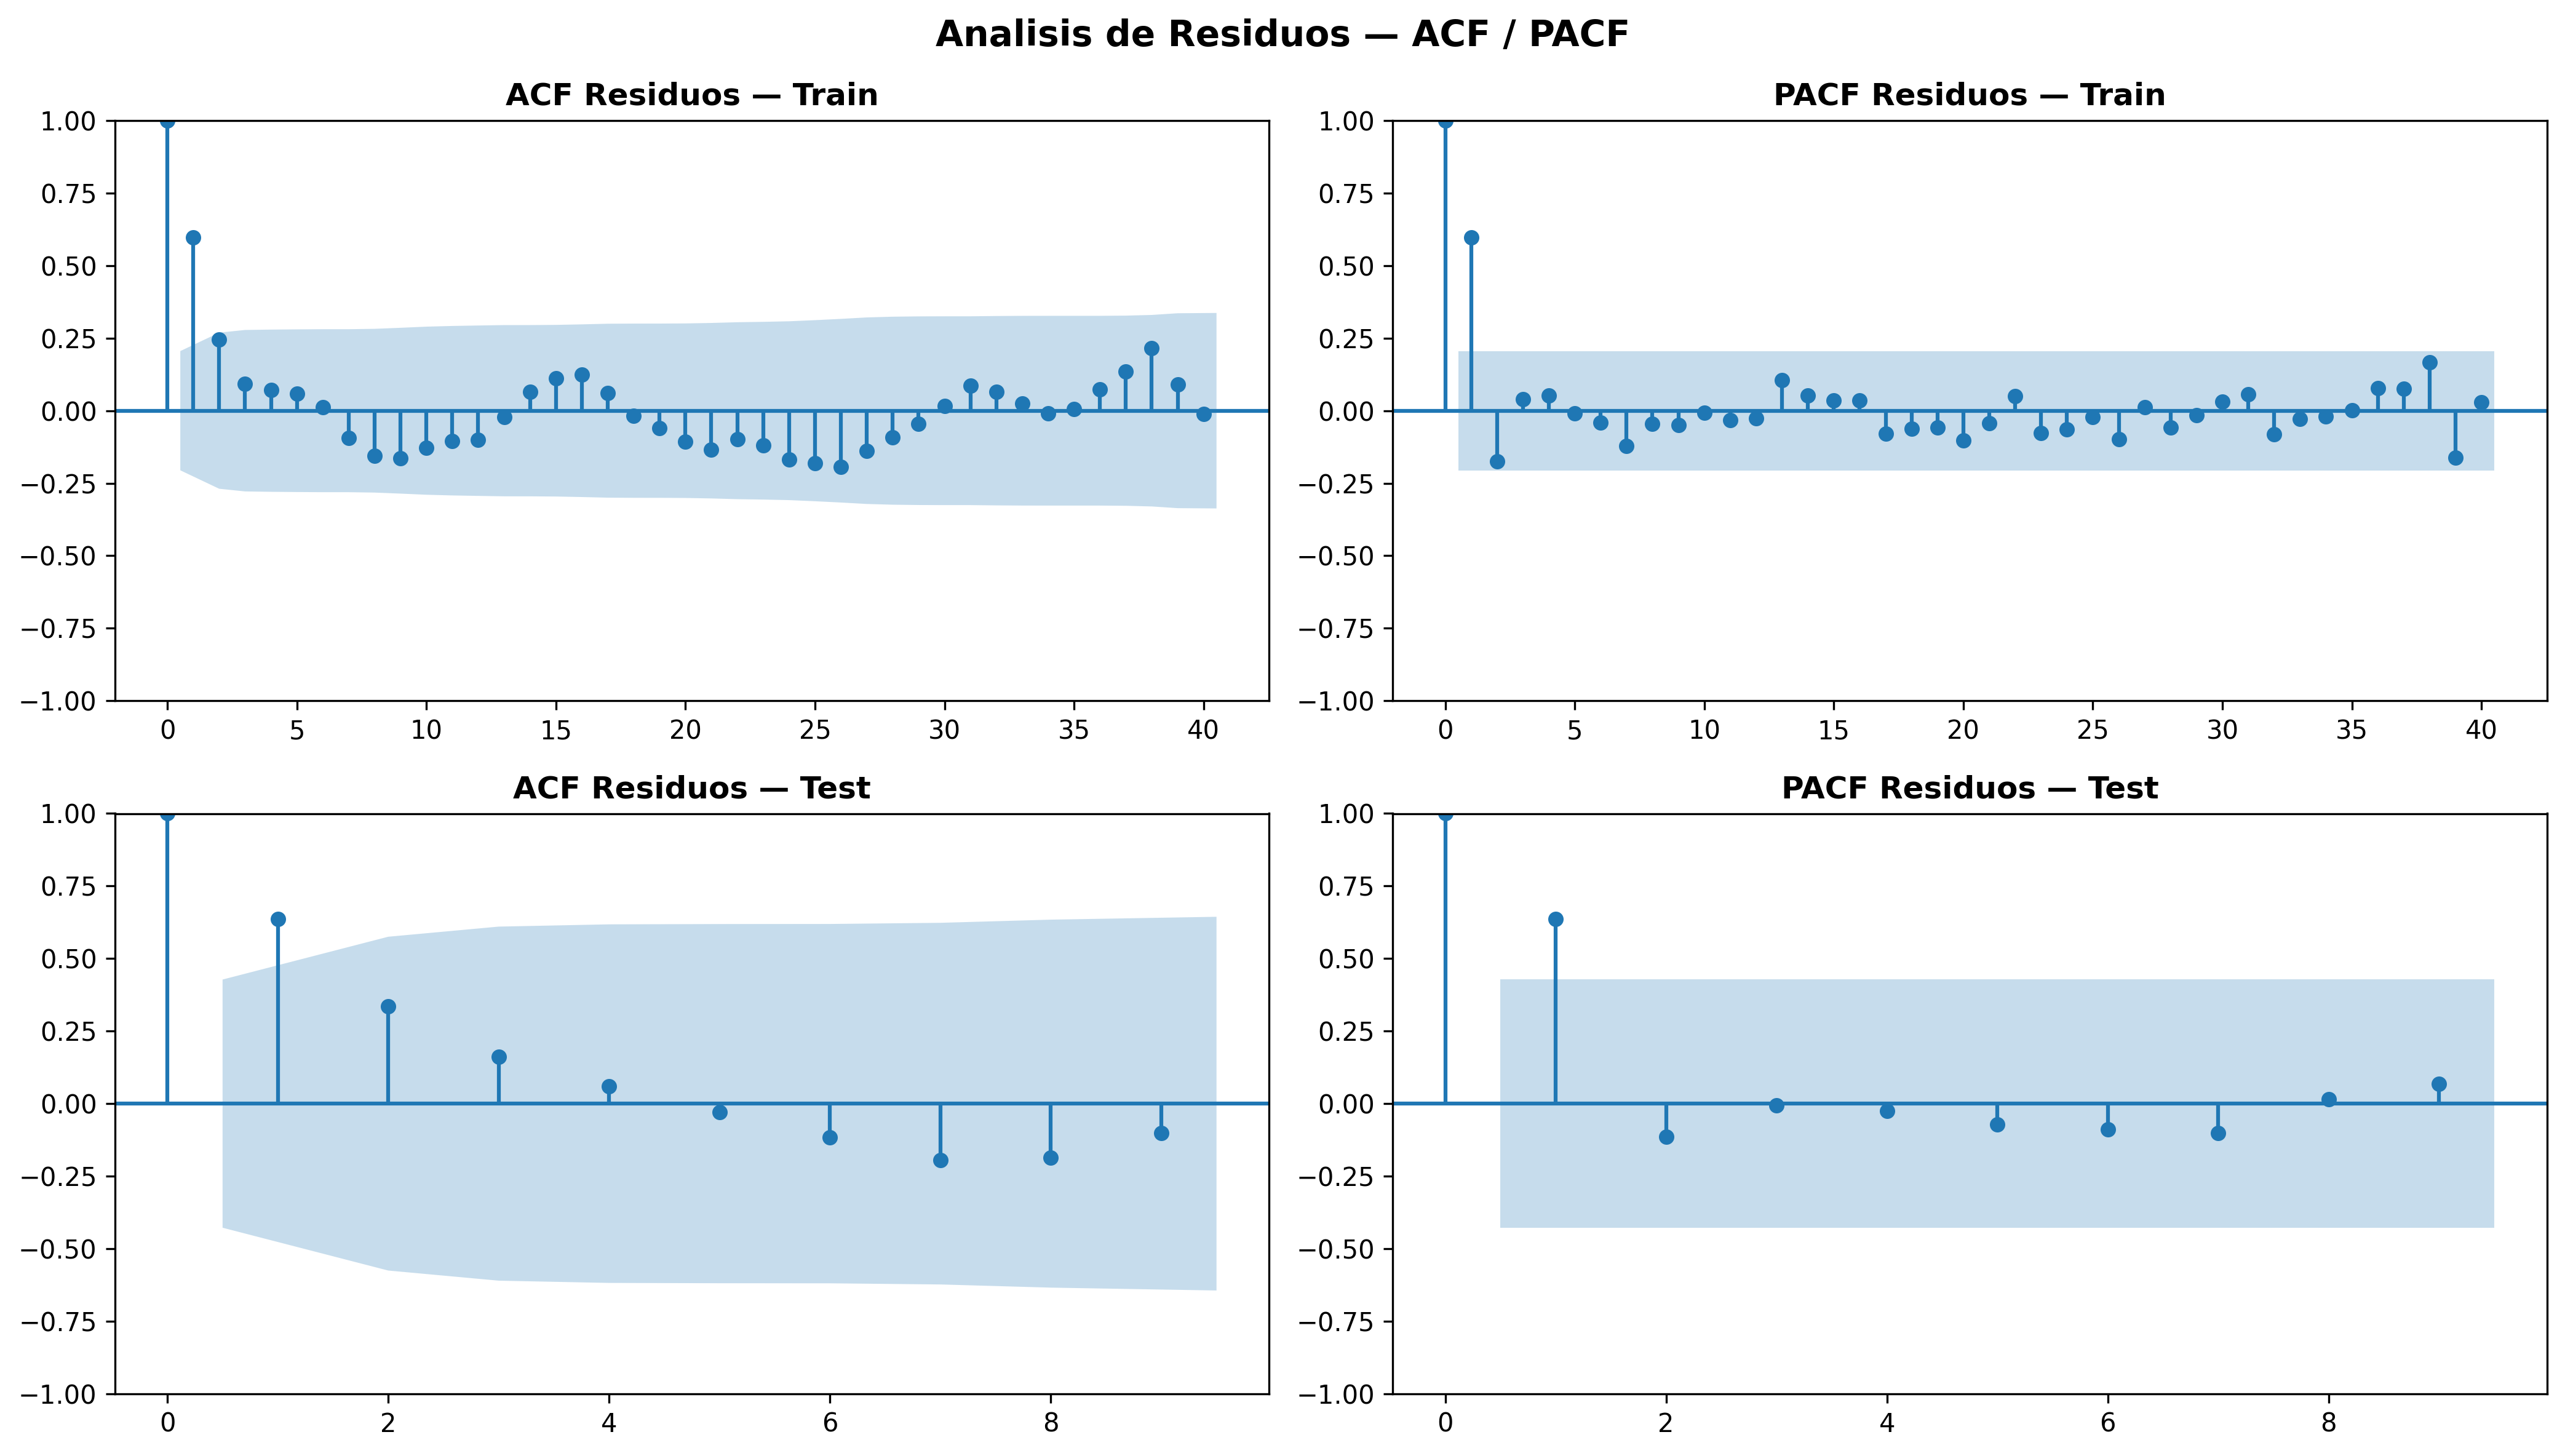
\includegraphics[width=\textwidth]{predicciones/prediccion_ladrillo_lstm/resultados_con_covid/residuos_acf_pacf.png}
    \caption{ACF y PACF de los residuos del modelo LSTM para ladrillo --- escenario con pandemia.}
    \label{fig:lstm_ladrillo_resacf_cc}
\end{figure}

\justify
El test de Ljung-Box sobre los residuos del conjunto de prueba muestra un $p$-valor de 0,077 a 10 rezagos (no rechaza $H_0$) y un $p$-valor de $6{,}70 \times 10^{-9}$ a 20 rezagos (rechaza fuertemente $H_0$). Al igual que en el escenario sin pandemia, los residuos se comportan como ruido blanco en los primeros rezagos pero muestran dependencia en rezagos más distantes.

\clearpage
\paragraph{Pronóstico a 24 Meses}

\begin{figure}[htbp]
    \centering
    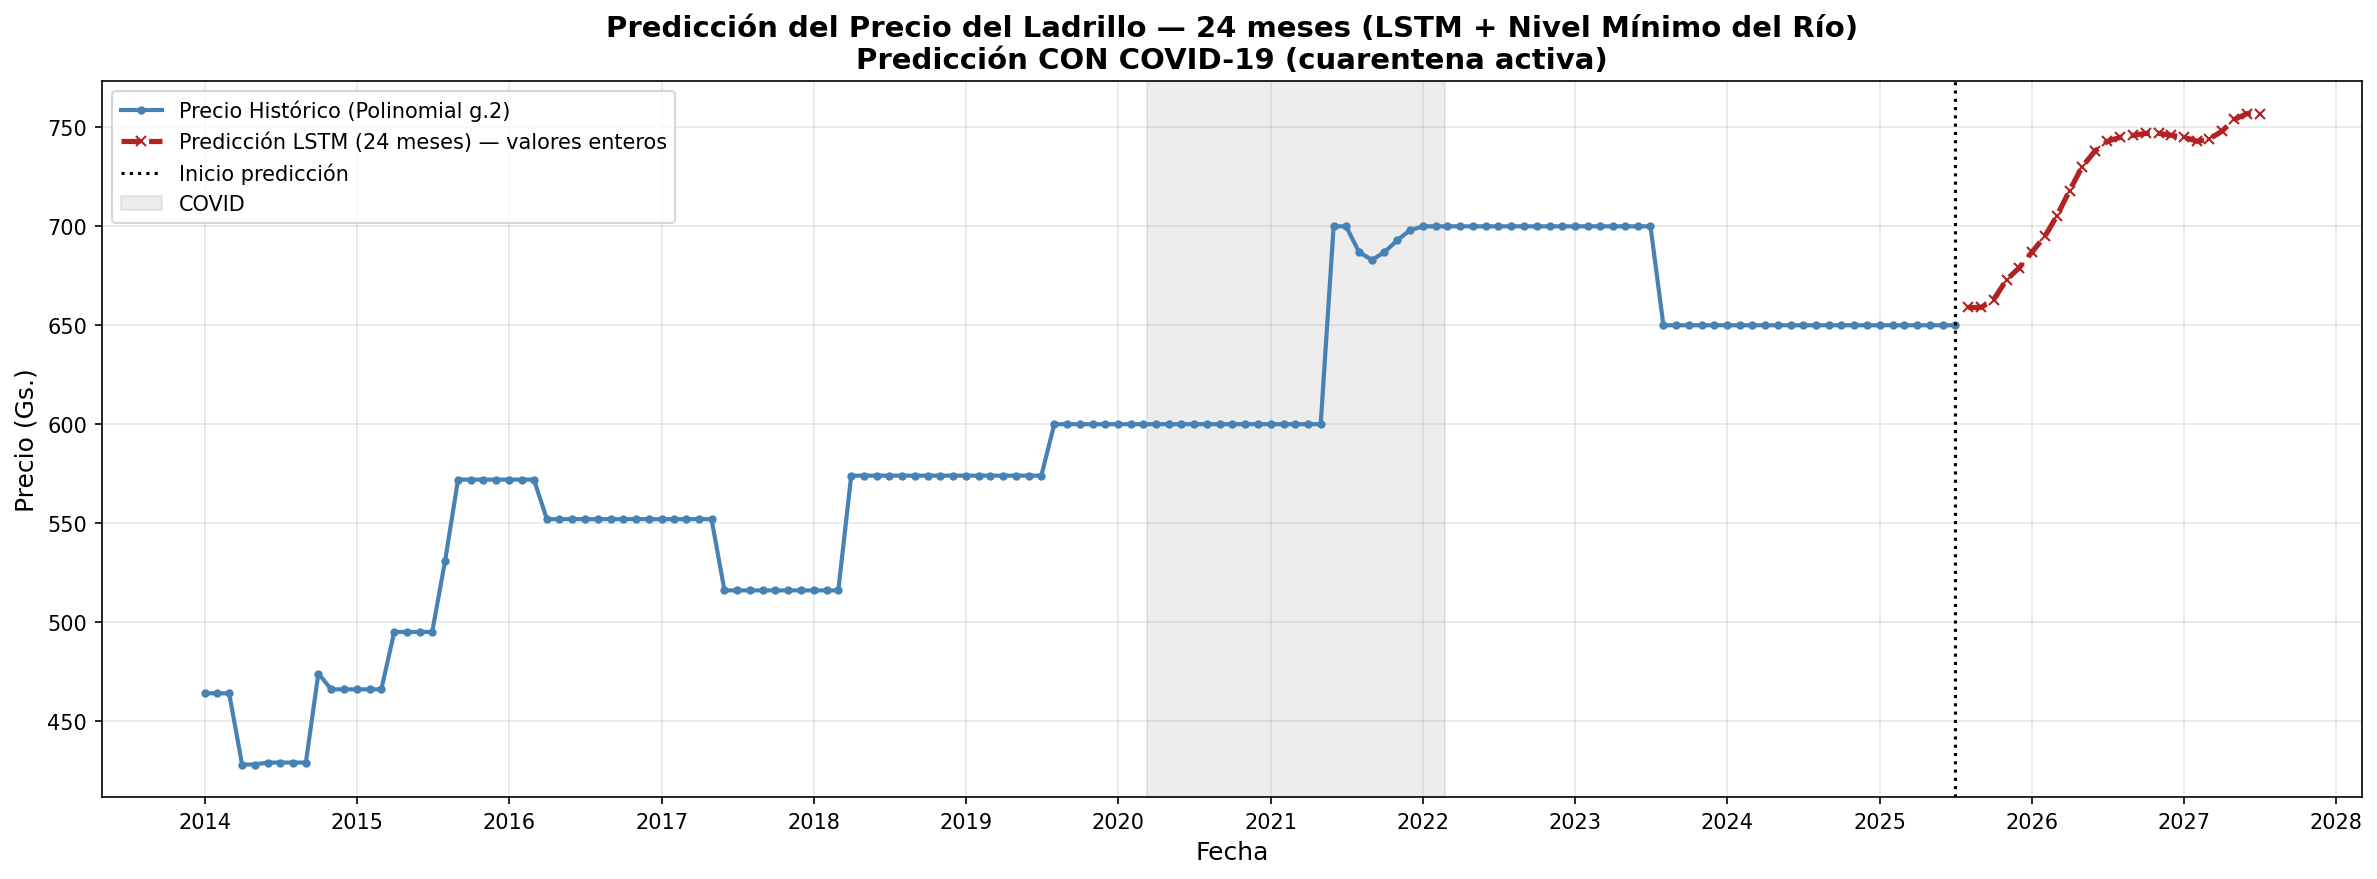
\includegraphics[width=\textwidth]{predicciones/prediccion_ladrillo_lstm/resultados_con_covid/final_06_prediccion_futura_completa.png}
    \caption{Pronóstico LSTM a 24 meses del precio del ladrillo --- escenario con pandemia, con IC al 95\,\%.}
    \label{fig:lstm_ladrillo_pred_con_covid}
\end{figure}

\begin{figure}[htbp]
    \centering
    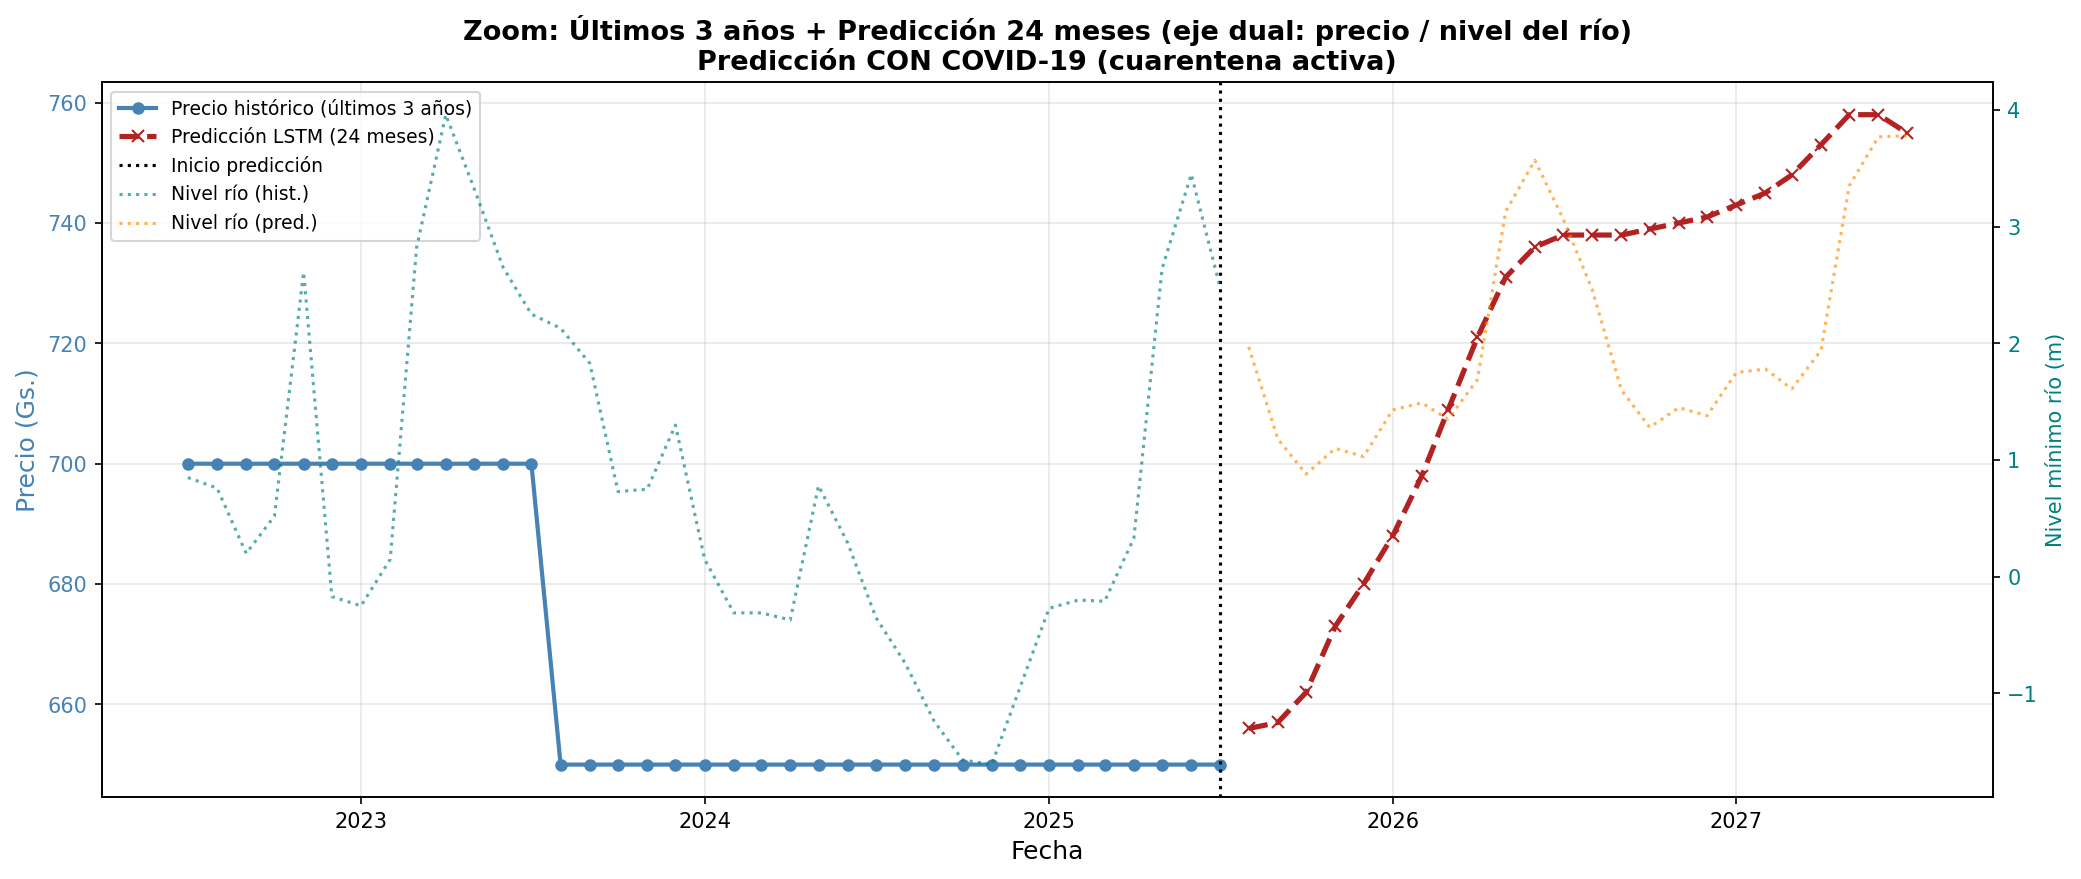
\includegraphics[width=\textwidth]{predicciones/prediccion_ladrillo_lstm/resultados_con_covid/final_07_prediccion_zoom_dual.png}
    \caption{Detalle de la transición histórico--pronóstico LSTM del ladrillo --- escenario con pandemia.}
    \label{fig:lstm_ladrillo_zoom_con_covid}
\end{figure}

\begin{figure}[htbp]
    \centering
    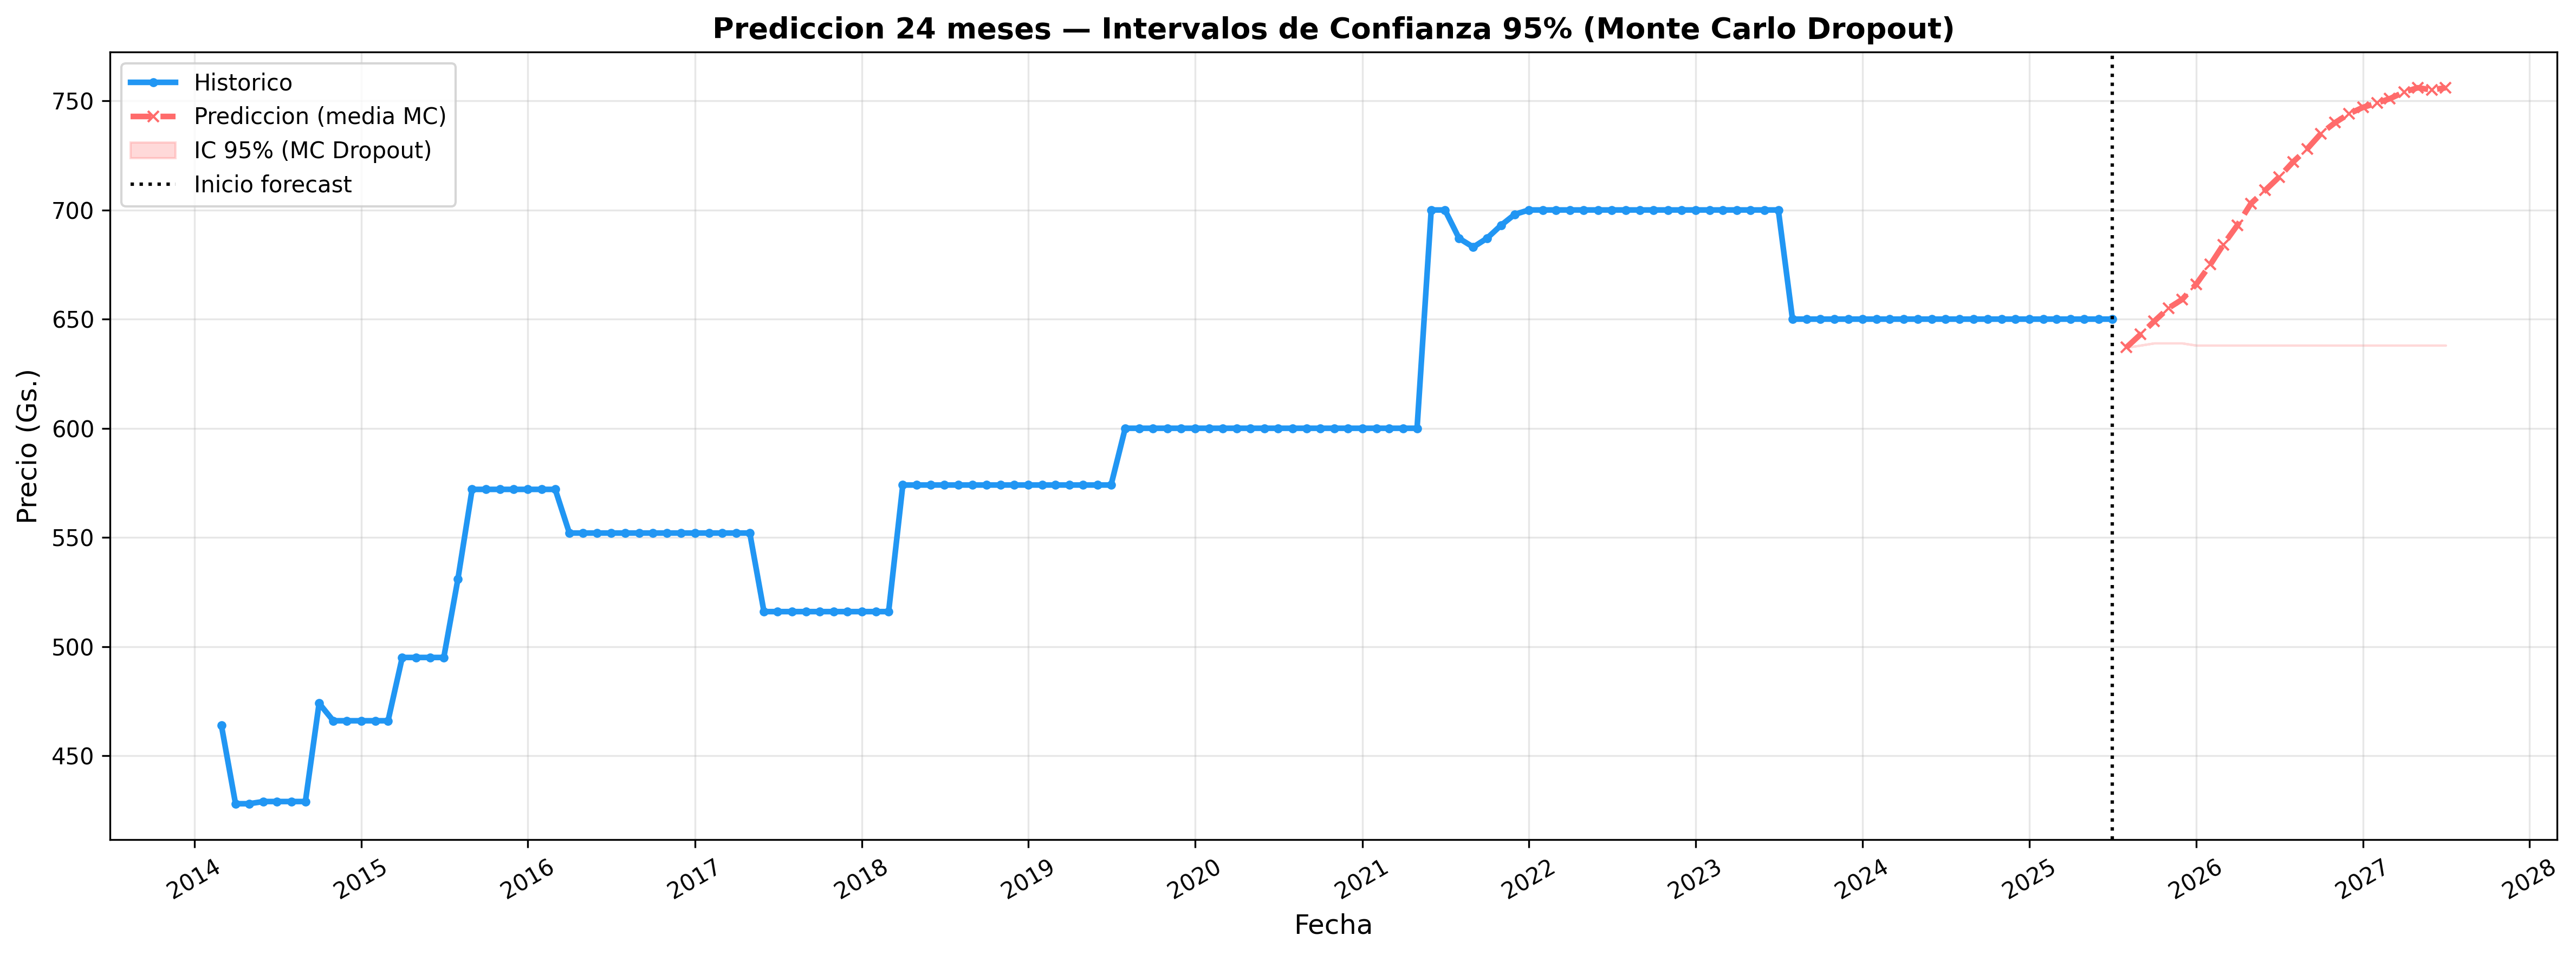
\includegraphics[width=\textwidth]{predicciones/prediccion_ladrillo_lstm/resultados_con_covid/forecast_ic_monte_carlo.png}
    \caption{IC Monte Carlo Dropout del pronóstico LSTM para ladrillo --- escenario con pandemia.}
    \label{fig:lstm_ladrillo_ic_mc_con_covid}
\end{figure}

\justify
Bajo el escenario con efecto pandémico, el rango de precios predicho se sitúa entre Gs.~637 y Gs.~756, con una dispersión considerablemente mayor que en el escenario sin pandemia. La comparación entre ambos escenarios muestra que el efecto pandémico eleva el precio máximo predicho del ladrillo de Gs.~644 a Gs.~756, un incremento del 17,4\,\% en el límite superior del rango. Este resultado indica que el modelo LSTM identifica un impacto alcista de las disrupciones pandémicas sobre el precio del ladrillo, aunque proporcionalmente menor que el efecto observado en el cemento (29,7\,\%). La menor magnitud puede atribuirse a que el ladrillo, como material de producción predominantemente local con cadenas de suministro más cortas, es menos sensible a las disrupciones logísticas internacionales.

% ============================================================
% SECCIÓN 4.4 — Predicción con GRU (Cemento + Ladrillo)
% ============================================================
\section{Predicción de los Precios del Cemento y del Ladrillo Común con Gated Recurrent Unit (GRU)}
\vspace{0.3cm}

\justify
Como alternativa al modelo LSTM, se evaluó la arquitectura \textit{Gated Recurrent Unit} (GRU), propuesta por Cho et al.\ (2014) como una simplificación de las redes LSTM. A diferencia de la celda LSTM, que emplea tres compuertas (entrada, olvido y salida), la celda GRU utiliza únicamente dos ---la de actualización (\textit{update gate}) y la de reinicio (\textit{reset gate})---, lo que reduce el número de parámetros entrenables y puede favorecer la convergencia en \textit{datasets} de tamaño moderado.

\justify
Al igual que para el LSTM, para cada material se entrenaron dos modelos GRU independientes: uno para el escenario sin efecto pandémico y otro para el escenario con efecto pandémico. Los hiperparámetros de cada modelo fueron optimizados de forma independiente con Optuna. La implementación se realizó con TensorFlow 2.19.0 / Keras, con la misma partición temporal (95 / 20 / 22 meses), las mismas 7 variables de entrada y los mismos intervalos de confianza al 95\,\% estimados por Monte Carlo Dropout ($N=100$ simulaciones). Dado que cada escenario puede resultar en arquitecturas distintas, los resultados de cada uno se presentan por separado.

% ============================================================
% 4.4.1 — CEMENTO GRU
% ============================================================
\subsection{Predicción del Precio del Cemento}

\justify
Para el cemento, ambos escenarios resultaron en modelos GRU con diferente configuración de hiperparámetros y distintas métricas de evaluación. A continuación se presenta cada escenario con su propia descripción completa.

% ------ CEMENTO GRU SIN COVID ------
\subsubsection{Escenario sin Efecto Pandémico}

\paragraph{Hiperparámetros y Arquitectura}

\justify
La búsqueda de hiperparámetros con Optuna para el escenario sin pandemia seleccionó una capa GRU unidireccional con 64 unidades ocultas, ventana de entrada (\textit{lookback}) de 6 meses, optimizador Adam con tasa de aprendizaje $\eta = 0{,}00732$ y \textit{weight decay} de $2{,}60 \times 10^{-7}$, \textit{batch size} de 2, \textit{dropout} de 0{,}1, \textit{dropout} recurrente de 0{,}0, y \textit{scheduler} ReduceLROnPlateau. La arquitectura resultante totaliza 14.081 parámetros entrenables. La Tabla~\ref{tab:gru_cemento_sc_arq} resume los hiperparámetros seleccionados.

\begin{table}[htbp]
    \centering
    \caption{Hiperparámetros del modelo GRU para cemento --- escenario sin pandemia.}
    \label{tab:gru_cemento_sc_arq}
    \begin{tabular}{ll}
        \toprule
        \textbf{Hiperparámetro} & \textbf{Valor} \\
        \midrule
        Capas GRU              & 1 (unidireccional) \\
        Unidades ocultas       & 64 \\
        Lookback               & 6 meses \\
        Optimizador            & Adam ($\eta=0{,}00732$, WD $=2{,}60 \times 10^{-7}$) \\
        Batch size             & 2 \\
        Dropout / Rec.\ dropout & 0{,}1 / 0{,}0 \\
        Scheduler              & ReduceLROnPlateau \\
        Parámetros entrenables & 14.081 \\
        \bottomrule
    \end{tabular}
\end{table}

\paragraph{Curva de Aprendizaje}

\justify
El modelo GRU del cemento para el escenario sin pandemia convergió en 35 épocas con \textit{early stopping}. La Figura~\ref{fig:gru_cemento_curva_sc} muestra las curvas de pérdida de entrenamiento y validación. Se observa un descenso rápido de ambas curvas durante las primeras 10 épocas, seguido de una estabilización gradual sin signos evidentes de sobreajuste.

\begin{figure}[htbp]
    \centering
    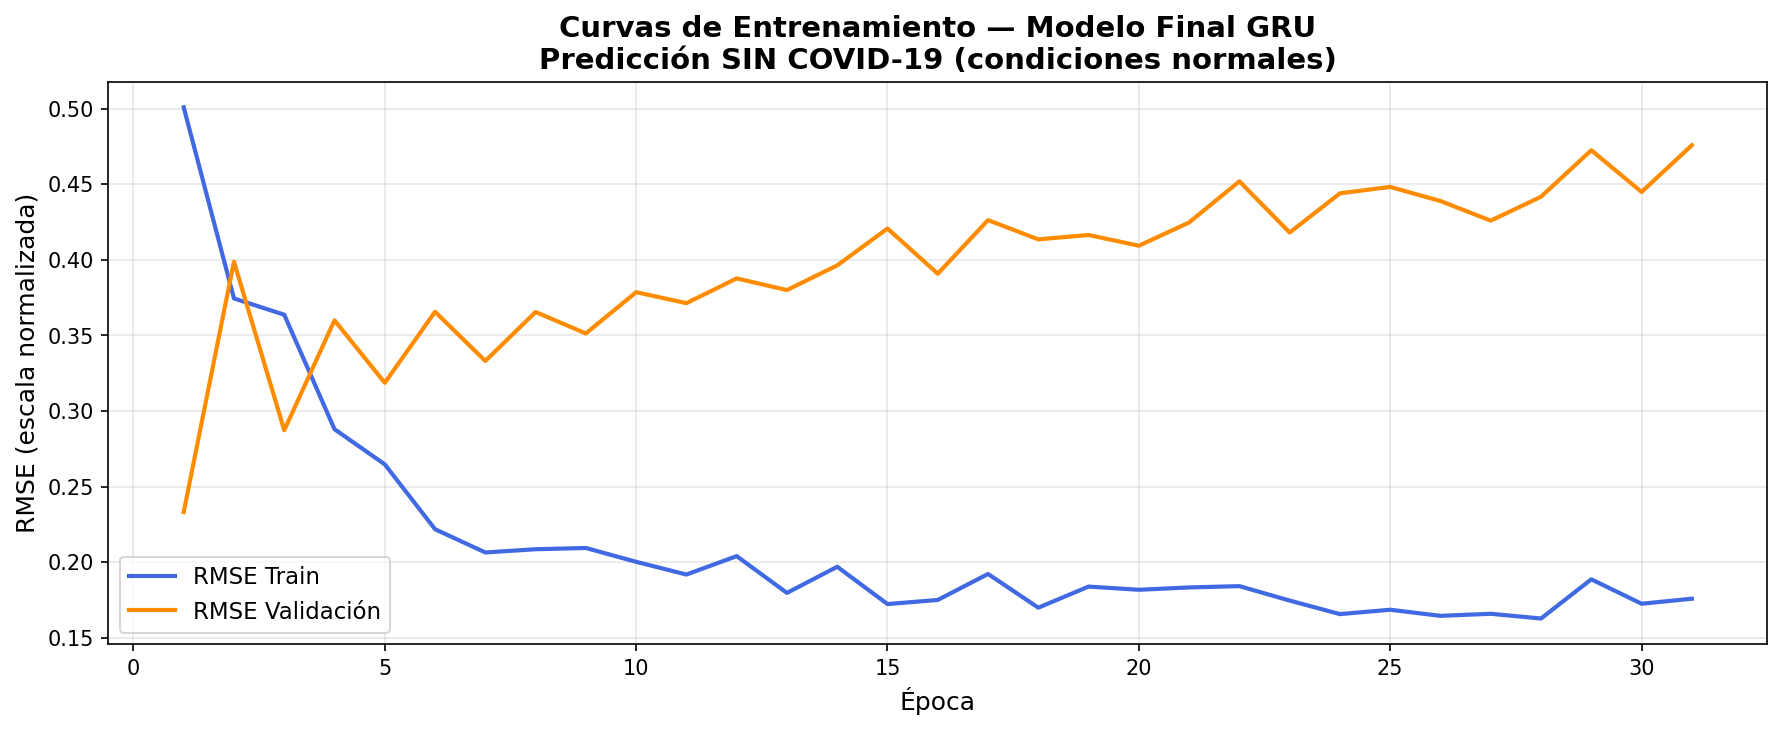
\includegraphics[width=\textwidth]{predicciones/prediccion_cemento_gru/resultados_sin_covid/final_01_curvas_entrenamiento.png}
    \caption{Curvas de aprendizaje del modelo GRU para cemento --- escenario sin pandemia.}
    \label{fig:gru_cemento_curva_sc}
\end{figure}

\paragraph{Métricas de Evaluación}

\begin{table}[htbp]
    \centering
    \caption{Desempeño del modelo GRU para cemento --- escenario sin pandemia: RMSE en train, val y test.}
    \label{tab:gru_cemento_sc_metricas}
    \begin{tabular}{lrrr}
        \toprule
        \textbf{Métrica} & \textbf{Train} & \textbf{Val} & \textbf{Test} \\
        \midrule
        RMSE (Gs.) & 4.911{,}67 & 2.862{,}84 & 2.709{,}13 \\
        \bottomrule
    \end{tabular}
\end{table}

\justify
El RMSE sobre el conjunto de prueba (Gs.~2.709{,}13) es inferior al RMSE de entrenamiento (Gs.~4.911{,}67) y al de validación (Gs.~2.862{,}84), patrón que indica ausencia de sobreajuste. En términos relativos al rango histórico de la serie (Gs.~48.000--76.036), el RMSE de prueba representa aproximadamente el 9,5\,\% del rango, resultado superior al obtenido por el modelo LSTM del mismo material en el mismo escenario (RMSE test: Gs.~1.619,75).

\paragraph{Evaluación sobre el Conjunto de Prueba}

\begin{figure}[htbp]
    \centering
    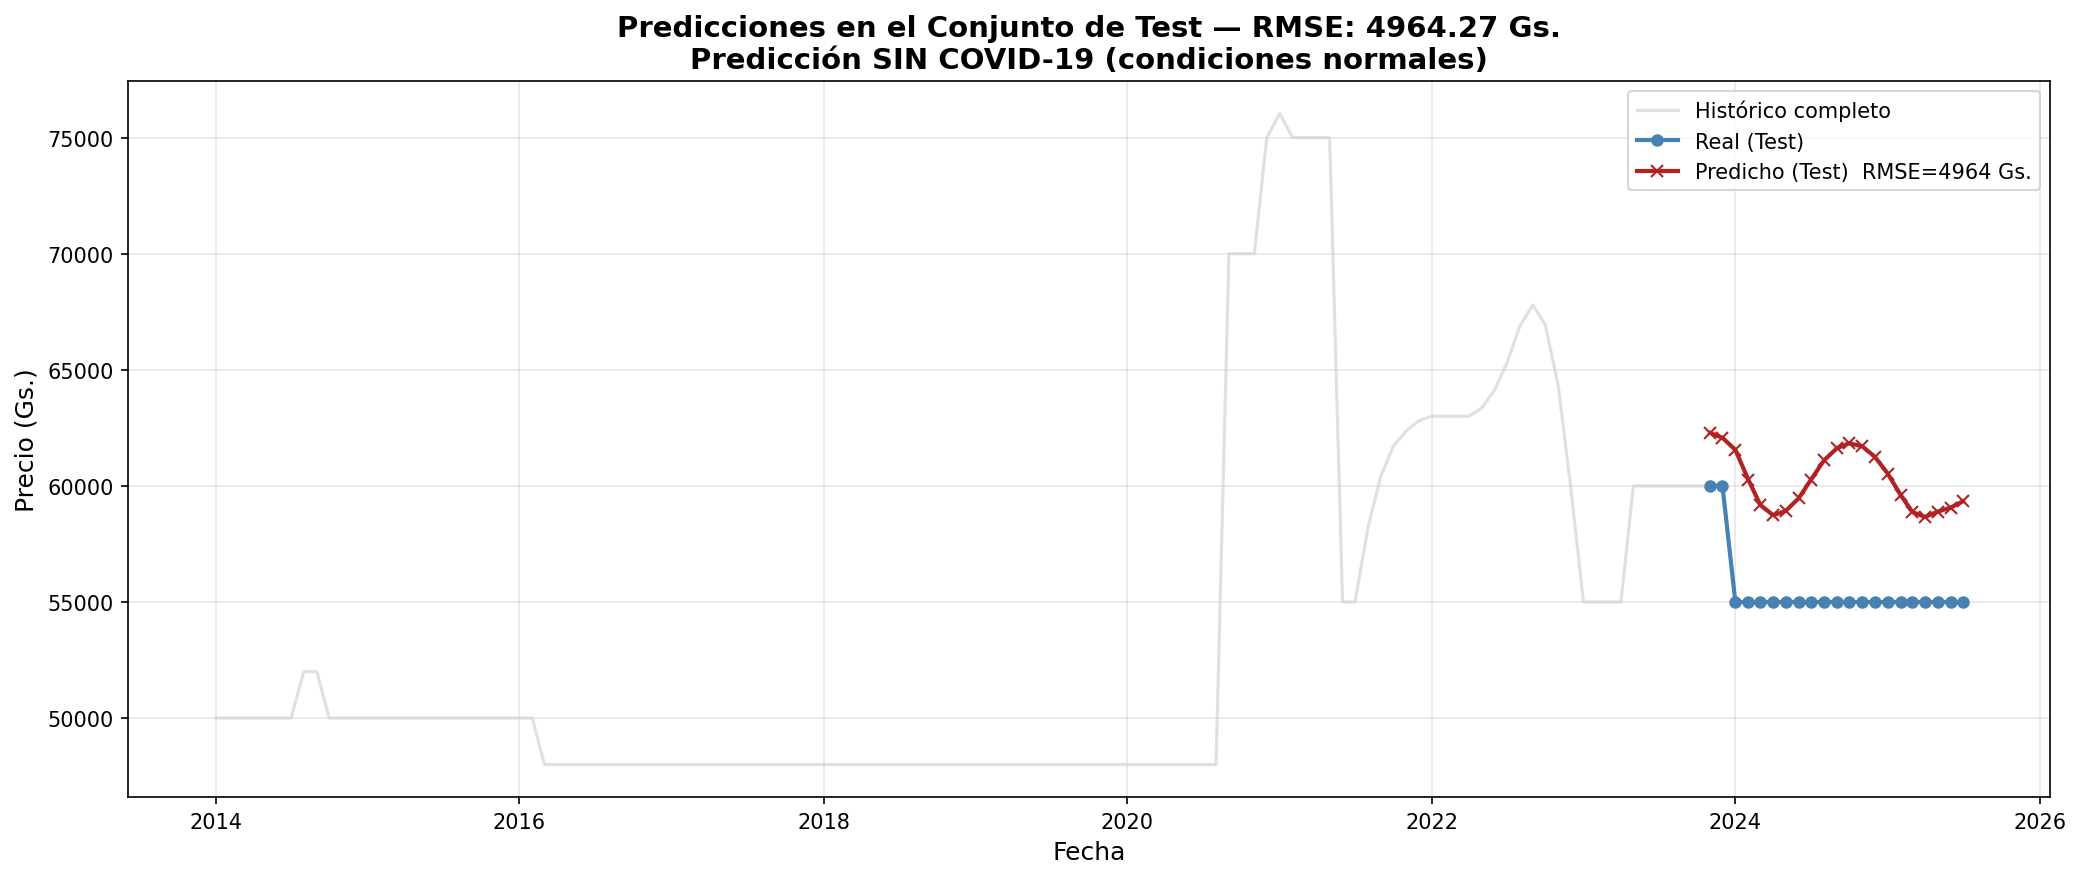
\includegraphics[width=\textwidth]{predicciones/prediccion_cemento_gru/resultados_sin_covid/final_02_prediccion_test_serie.png}
    \caption{Predicción GRU vs.\ valores reales del precio del cemento --- escenario sin pandemia, conjunto de prueba.}
    \label{fig:gru_cemento_test_sc}
\end{figure}

\begin{figure}[htbp]
    \centering
    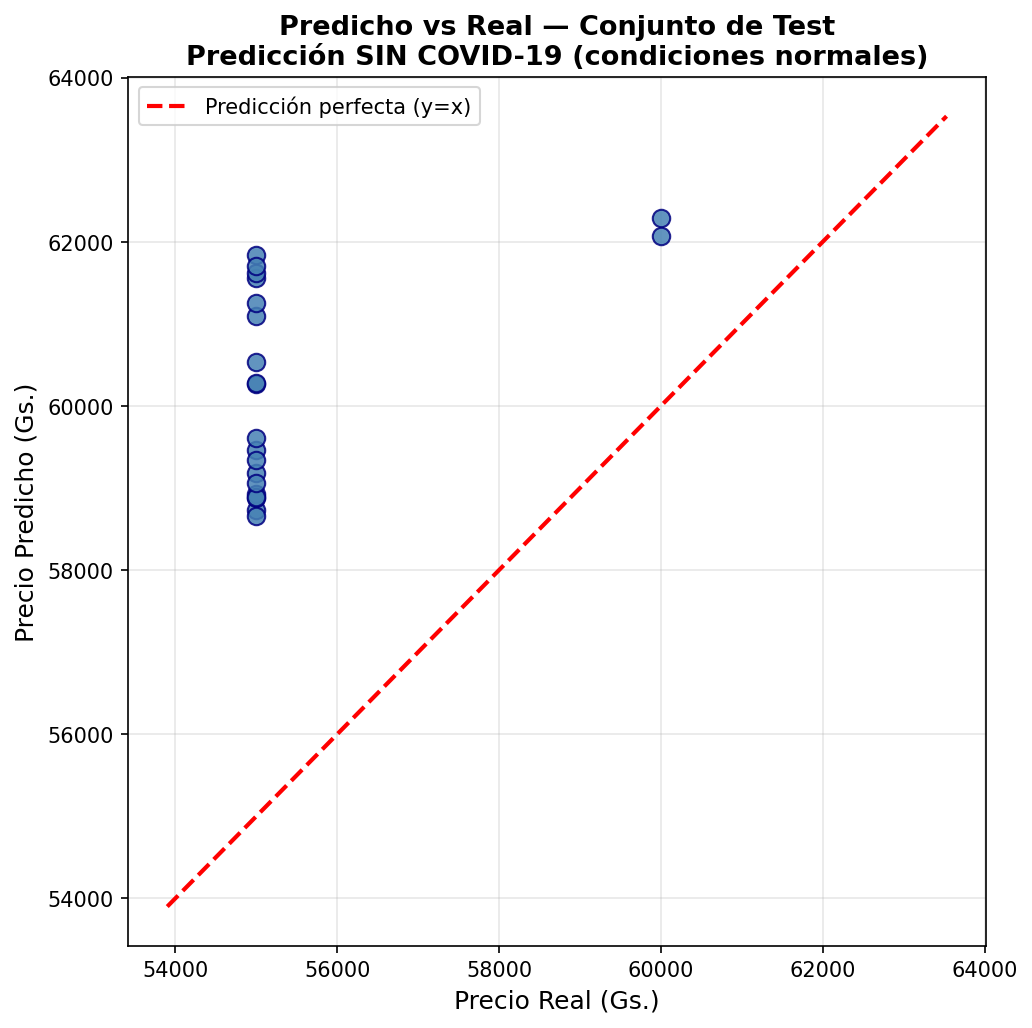
\includegraphics[width=0.8\textwidth]{predicciones/prediccion_cemento_gru/resultados_sin_covid/final_03_scatter_test.png}
    \caption{Diagrama de dispersión: precio predicho vs.\ real del cemento --- escenario sin pandemia (GRU).}
    \label{fig:gru_cemento_scatter_sc}
\end{figure}

\begin{figure}[htbp]
    \centering
    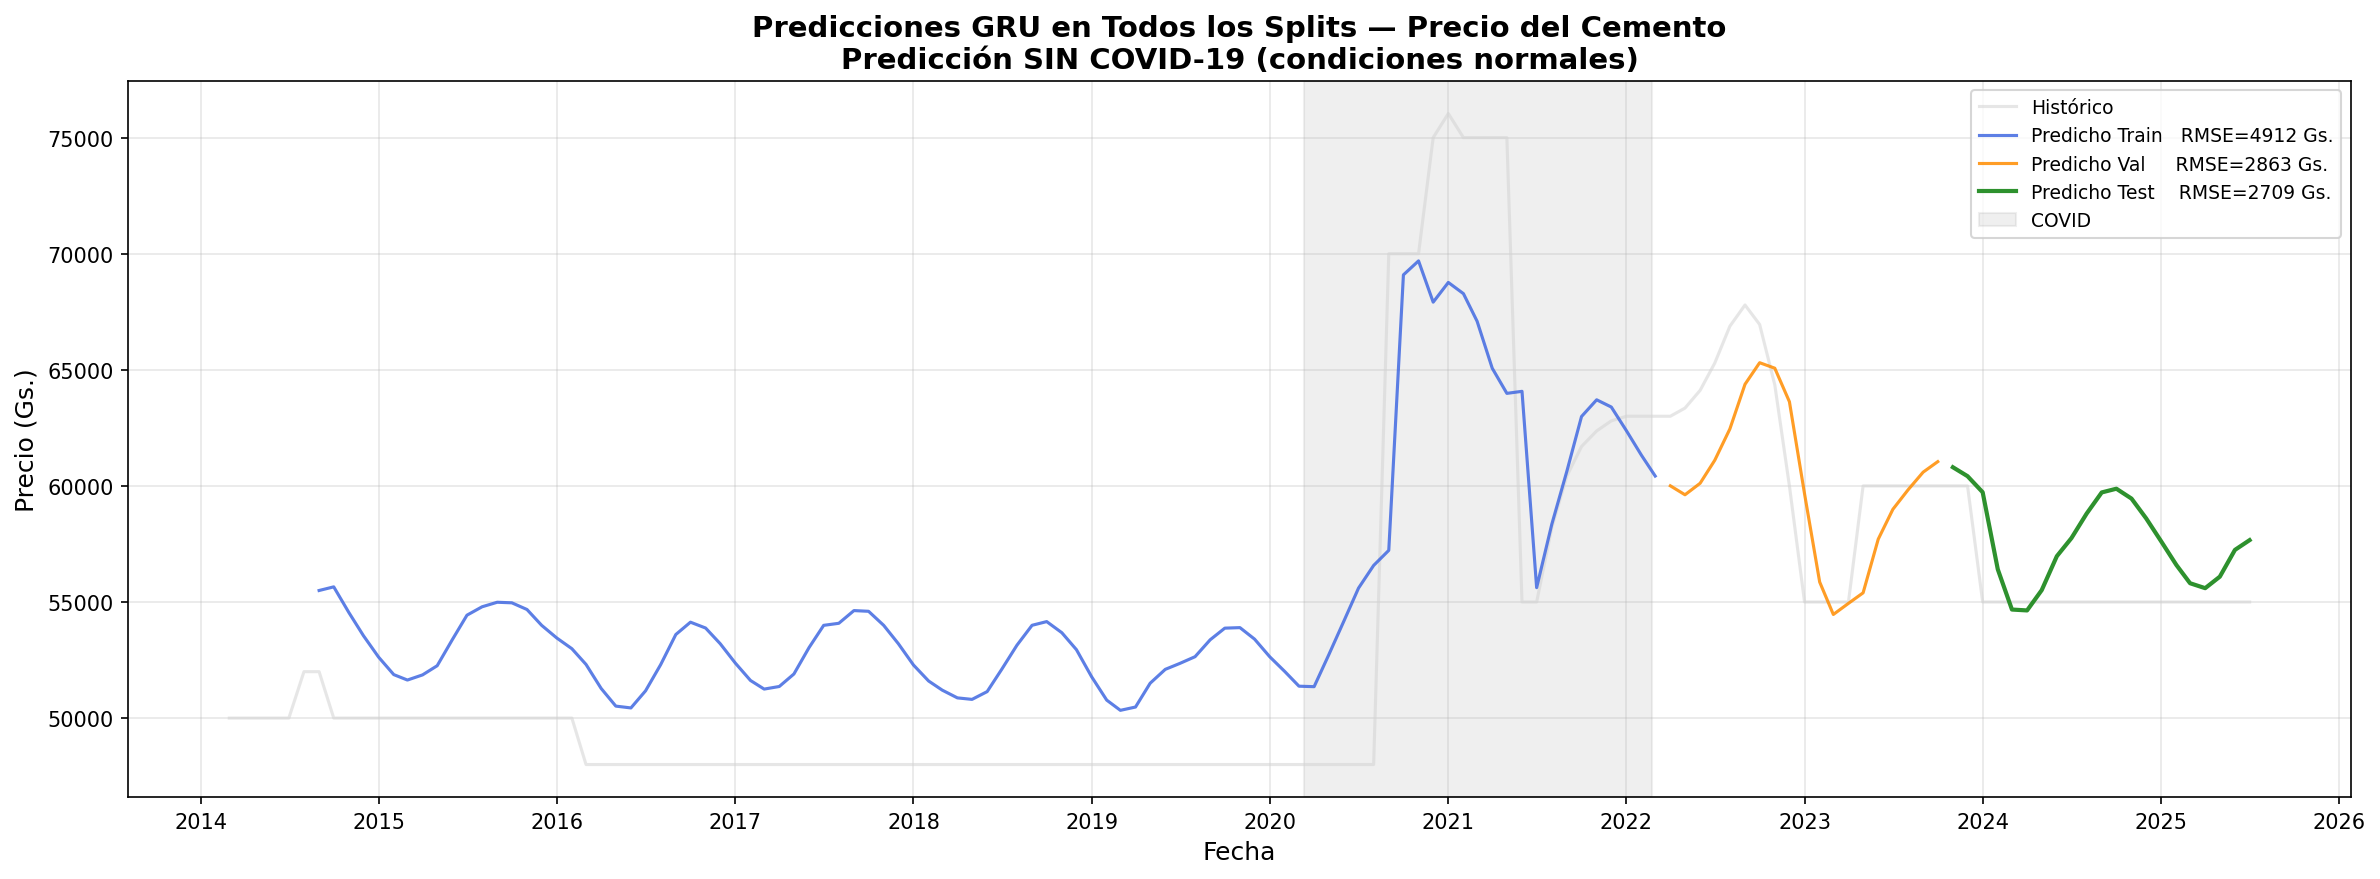
\includegraphics[width=\textwidth]{predicciones/prediccion_cemento_gru/resultados_sin_covid/final_05_todos_splits.png}
    \caption{Ajuste del modelo GRU del cemento sobre las tres particiones --- escenario sin pandemia.}
    \label{fig:gru_cemento_splits_sc}
\end{figure}

\clearpage
\paragraph{Análisis de Residuos}

\begin{figure}[htbp]
    \centering
    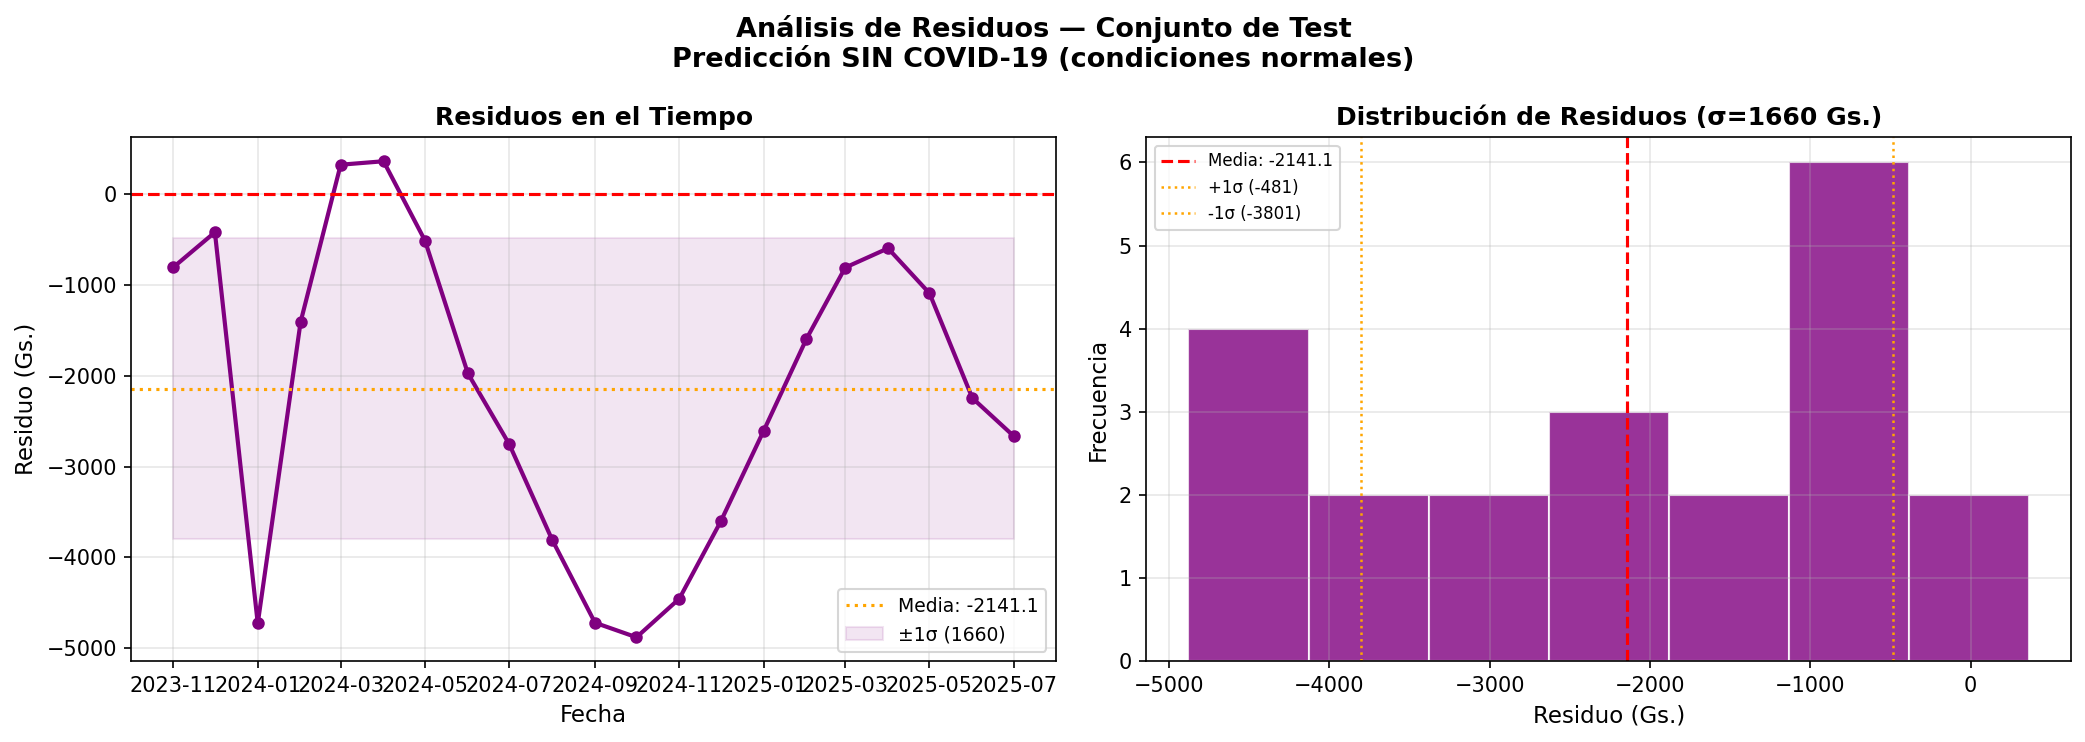
\includegraphics[width=\textwidth]{predicciones/prediccion_cemento_gru/resultados_sin_covid/final_04_residuos.png}
    \caption{Residuos del modelo GRU para cemento --- escenario sin pandemia, conjunto de prueba.}
    \label{fig:gru_cemento_res_sc}
\end{figure}

\begin{figure}[htbp]
    \centering
    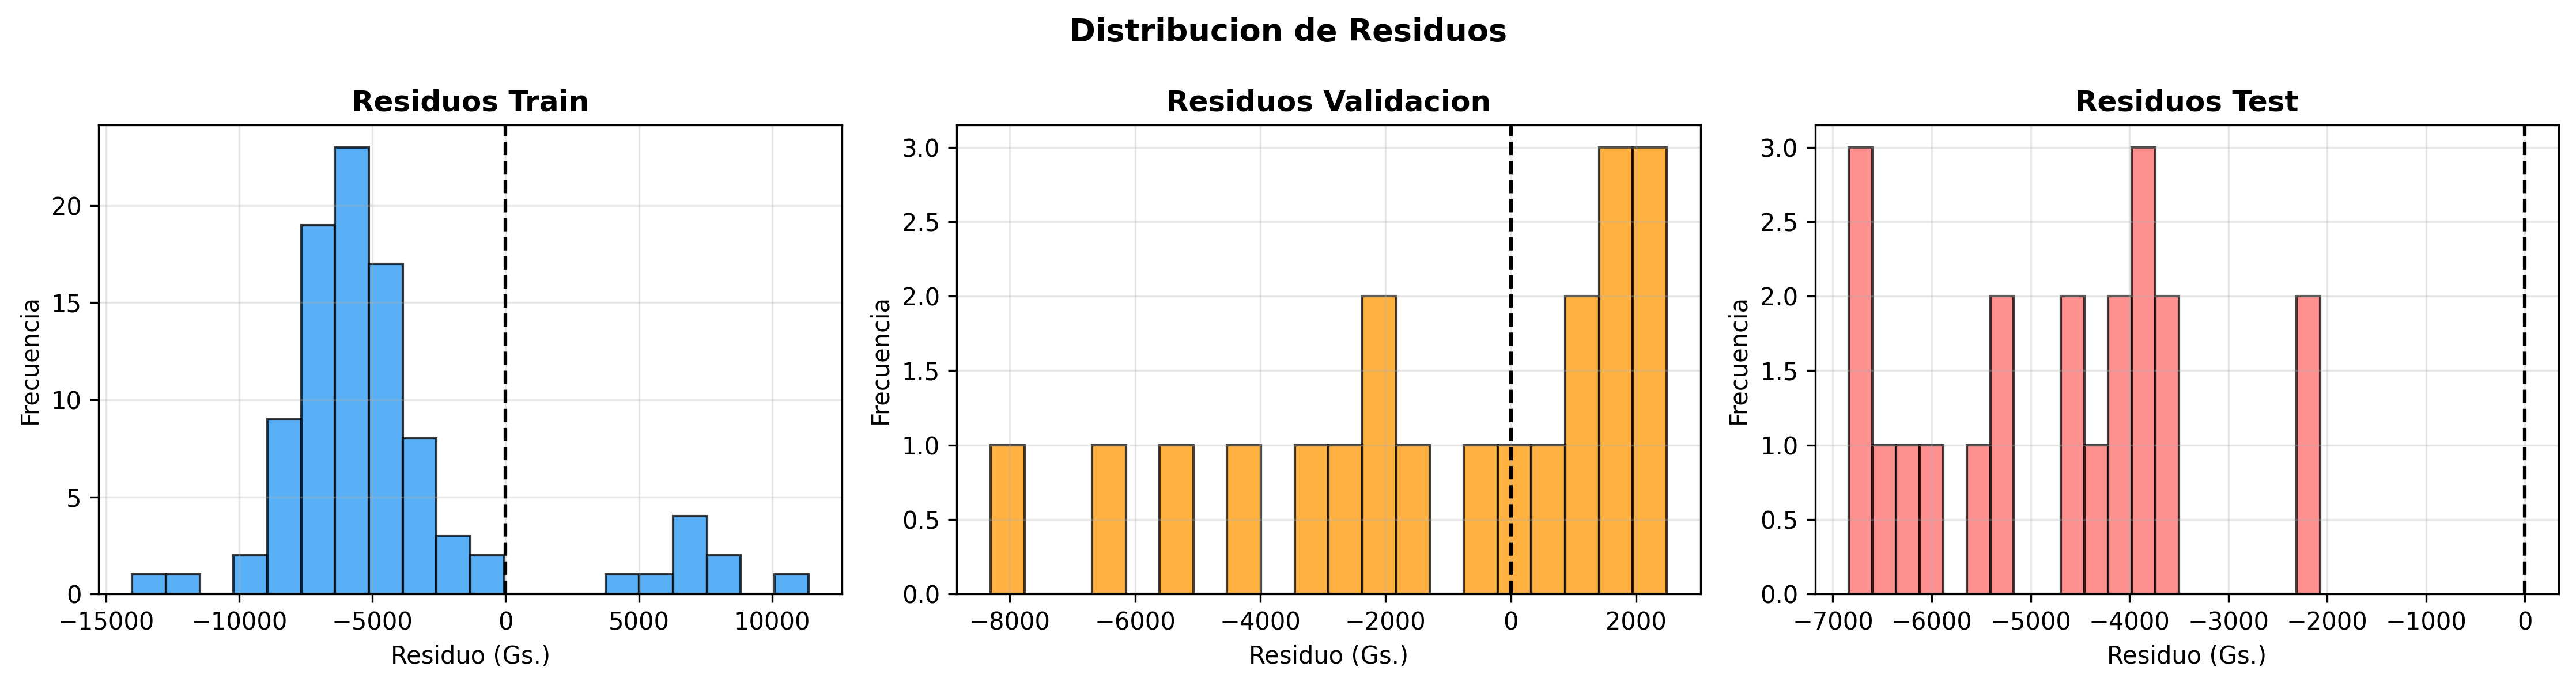
\includegraphics[width=0.8\textwidth]{predicciones/prediccion_cemento_gru/resultados_sin_covid/residuos_histograma.png}
    \caption{Histograma de residuos del modelo GRU para cemento --- escenario sin pandemia.}
    \label{fig:gru_cemento_reshist_sc}
\end{figure}

\begin{figure}[htbp]
    \centering
    \includegraphics[width=\textwidth]{predicciones/prediccion_cemento_gru/resultados_sin_covid/residuos_acf_pacf.png}
    \caption{ACF y PACF de los residuos del modelo GRU para cemento --- escenario sin pandemia.}
    \label{fig:gru_cemento_acf_sc}
\end{figure}

\justify
El test de Ljung-Box sobre los residuos del conjunto de prueba arroja un $p$-valor de 0,002 a 10 rezagos (rechaza $H_0$) y un $p$-valor de 0,077 a 20 rezagos (no rechaza $H_0$). Este resultado intermedio indica que el modelo captura la mayor parte de la estructura temporal, aunque persiste cierta dependencia serial de bajo orden en los primeros rezagos que no logra absorber completamente.

\clearpage
\paragraph{Pronóstico a 24 Meses}

\begin{figure}[htbp]
    \centering
    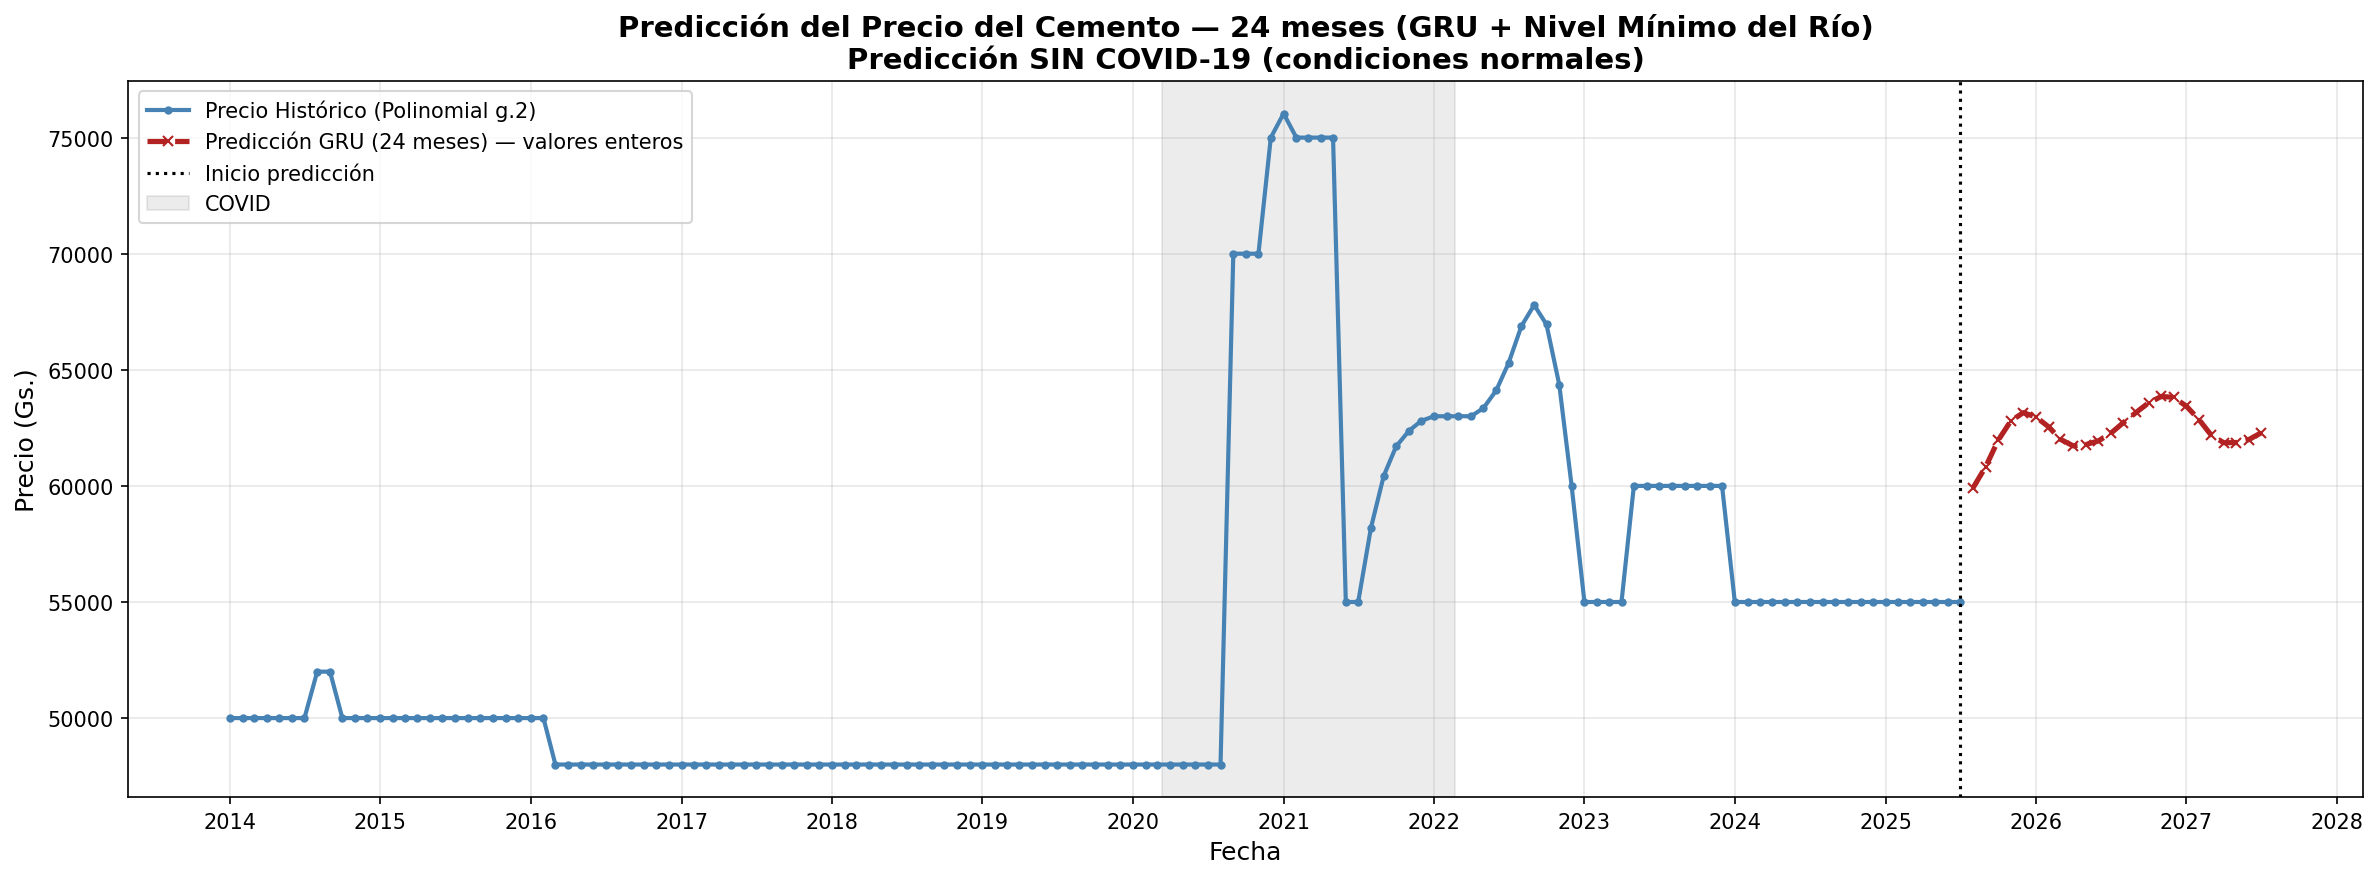
\includegraphics[width=\textwidth]{predicciones/prediccion_cemento_gru/resultados_sin_covid/final_06_prediccion_futura_completa.png}
    \caption{Pronóstico GRU del precio del cemento a 24 meses --- escenario sin pandemia: serie histórica y proyección.}
    \label{fig:gru_cemento_pred_sin_covid}
\end{figure}

\begin{figure}[htbp]
    \centering
    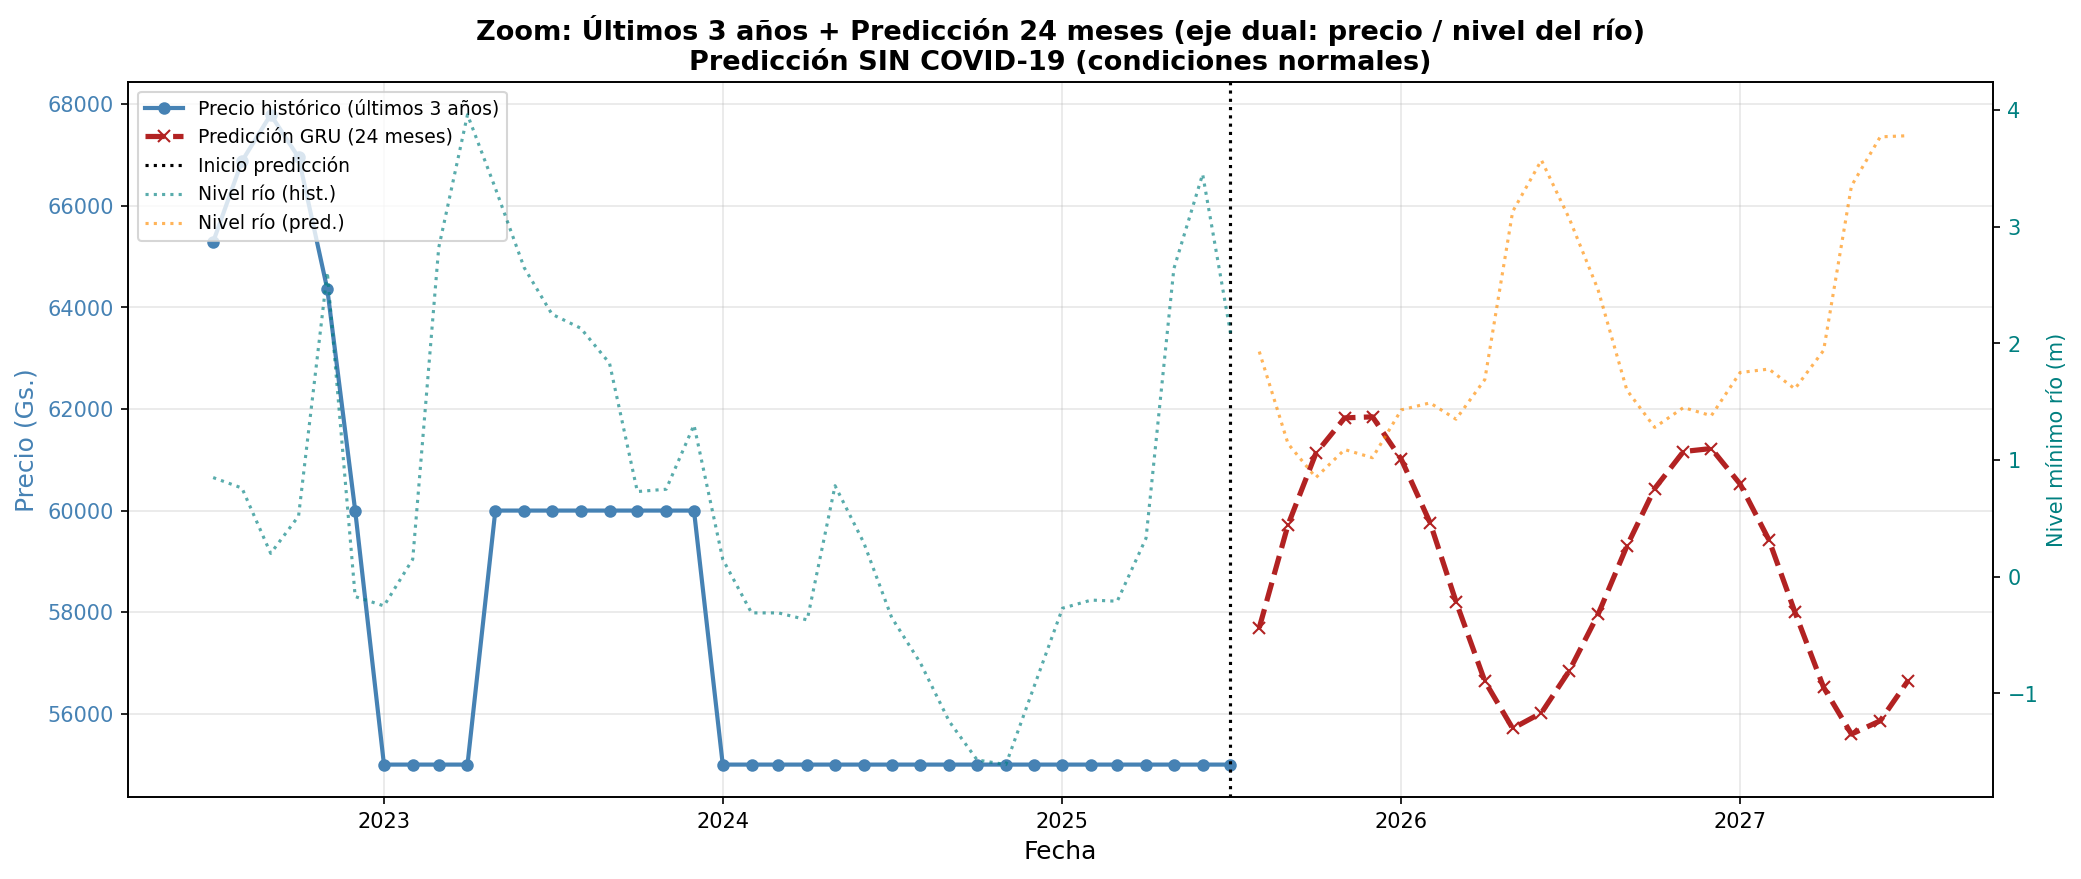
\includegraphics[width=\textwidth]{predicciones/prediccion_cemento_gru/resultados_sin_covid/final_07_prediccion_zoom_dual.png}
    \caption{Zoom sobre la transición entre datos observados y pronóstico GRU del cemento --- escenario sin pandemia.}
    \label{fig:gru_cemento_zoom_sin_covid}
\end{figure}

\begin{figure}[htbp]
    \centering
    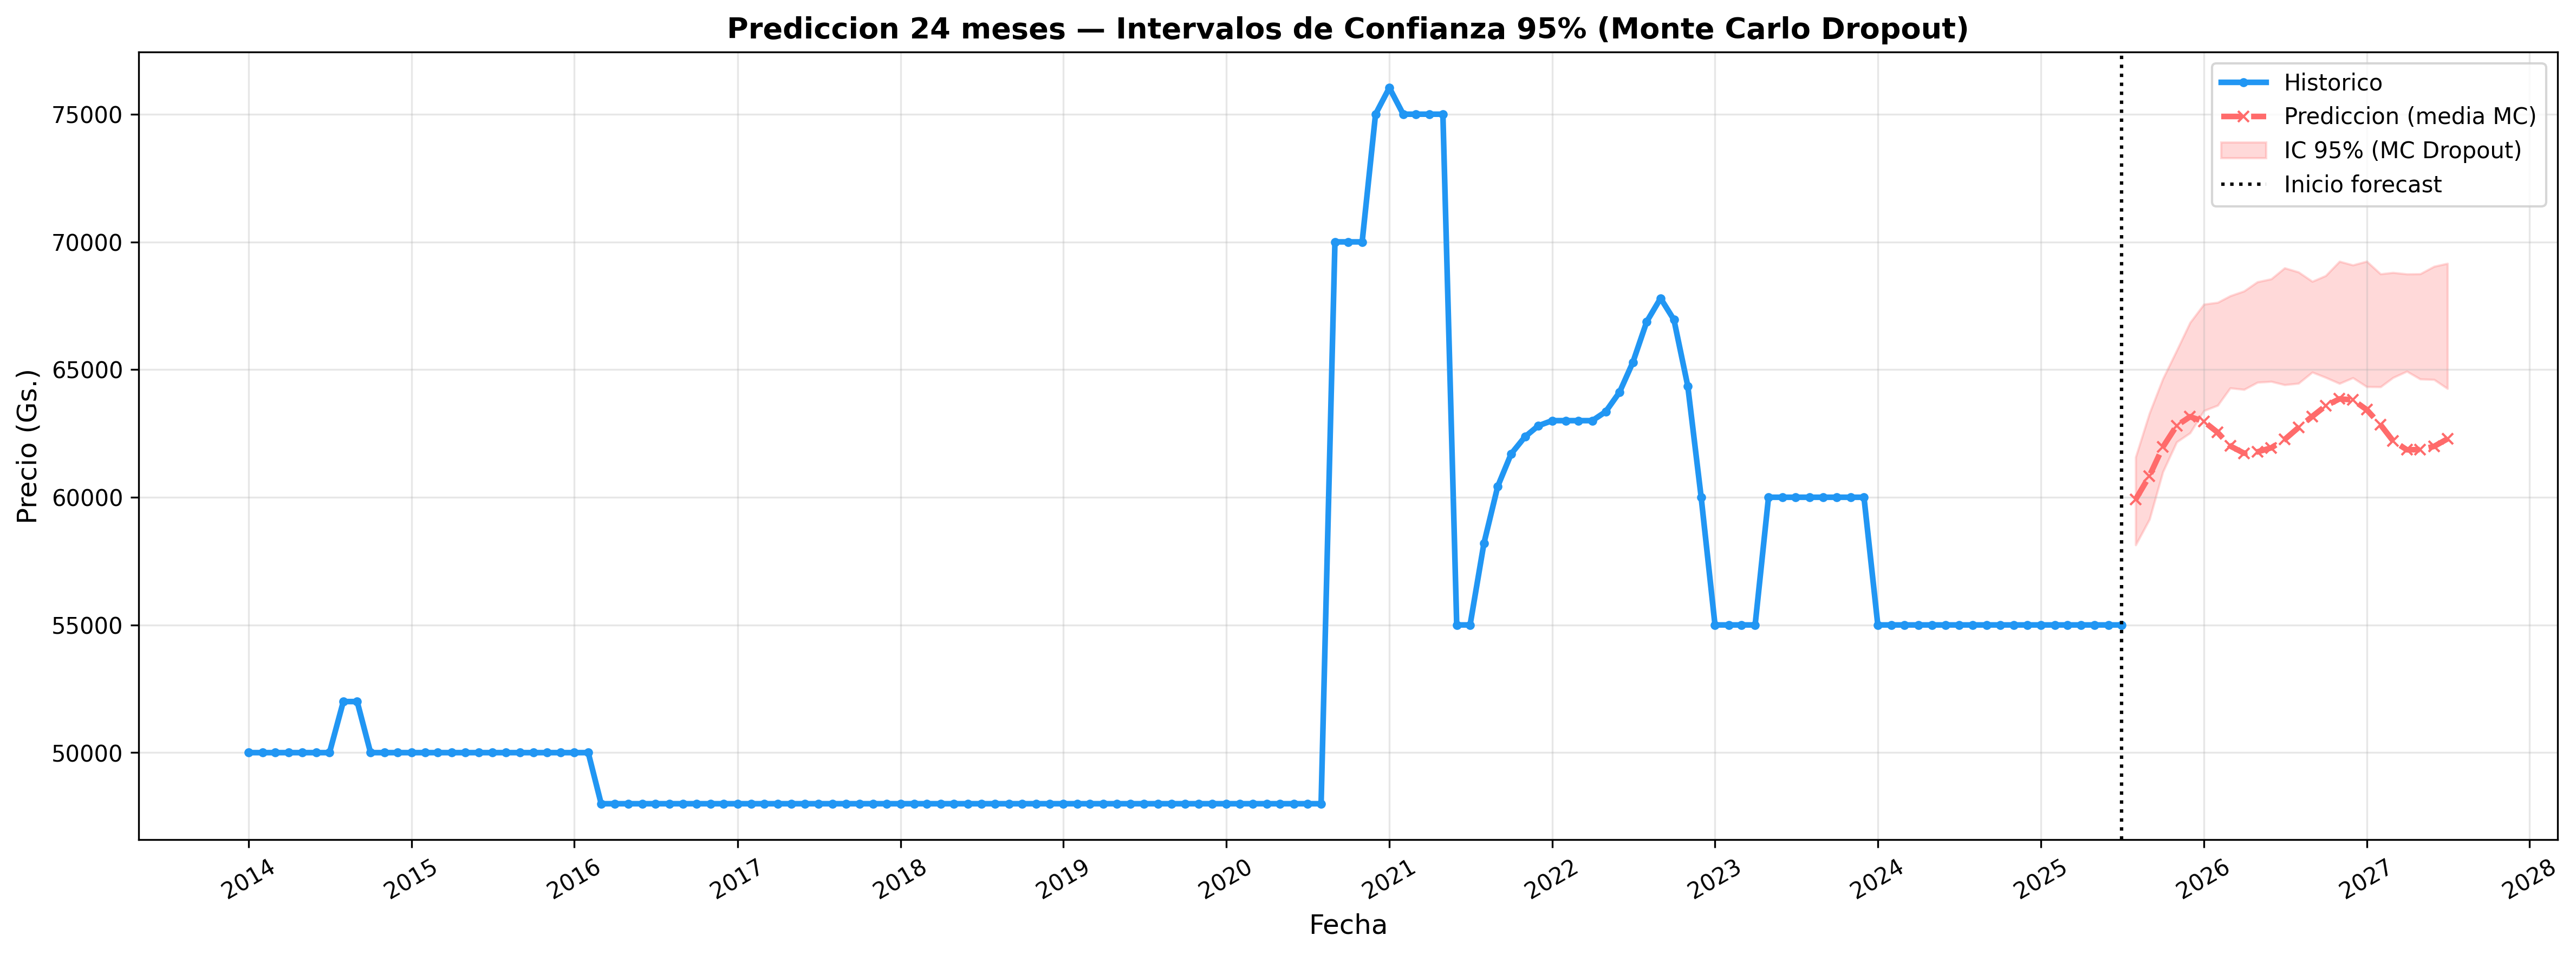
\includegraphics[width=\textwidth]{predicciones/prediccion_cemento_gru/resultados_sin_covid/forecast_ic_monte_carlo.png}
    \caption{IC Monte Carlo Dropout del pronóstico GRU para cemento --- escenario sin pandemia.}
    \label{fig:gru_cemento_ic_sin_covid}
\end{figure}

\justify
El modelo GRU proyecta, bajo el escenario sin pandemia, una tendencia ascendente del precio del cemento durante los primeros meses, alcanzando un máximo de Gs.~61.845 en diciembre de 2025, seguida de un descenso gradual hacia Gs.~55.712 en mayo de 2026 y una leve recuperación posterior. El rango de predicción para todo el horizonte se sitúa entre Gs.~55.600 y Gs.~61.845. La Tabla~\ref{tab:gru_cemento_pred_sc} sintetiza los valores pronosticados para los primeros doce meses.

\begin{table}[htbp]
    \centering
    \caption{Pronóstico GRU del precio del cemento (Gs.) --- escenario sin pandemia, agosto 2025 -- julio 2026.}
    \label{tab:gru_cemento_pred_sc}
    \begin{tabular}{lr}
        \toprule
        \textbf{Mes} & \textbf{Precio Predicho (Gs.)} \\
        \midrule
        Agosto 2025      & 57.693 \\
        Septiembre 2025  & 59.720 \\
        Octubre 2025     & 61.126 \\
        Noviembre 2025   & 61.824 \\
        Diciembre 2025   & 61.845 \\
        Enero 2026       & 61.009 \\
        Febrero 2026     & 59.763 \\
        Marzo 2026       & 58.206 \\
        Abril 2026       & 56.642 \\
        Mayo 2026        & 55.712 \\
        Junio 2026       & 56.018 \\
        Julio 2026       & 56.846 \\
        \bottomrule
    \end{tabular}
\end{table}

% ------ CEMENTO GRU CON COVID ------
\clearpage
\subsubsection{Escenario con Efecto Pandémico}

\paragraph{Hiperparámetros y Arquitectura}

\justify
Para el escenario con efecto pandémico, la búsqueda con Optuna convergió a una configuración diferente: una capa GRU unidireccional con 64 unidades ocultas, sin \textit{dropout} ni planificador de tasa de aprendizaje. El optimizador fue Adam con $\eta = 0{,}001$ y regularización L2 $\lambda=10^{-5}$, \textit{lookback} de 6 meses y \textit{batch size} de 4. La arquitectura resultante totaliza los mismos 14.081 parámetros entrenables, pero con una dinámica de entrenamiento más simple. La Tabla~\ref{tab:gru_cemento_cc_arq} resume estos parámetros.

\begin{table}[htbp]
    \centering
    \caption{Hiperparámetros del modelo GRU para cemento --- escenario con pandemia.}
    \label{tab:gru_cemento_cc_arq}
    \begin{tabular}{ll}
        \toprule
        \textbf{Hiperparámetro} & \textbf{Valor} \\
        \midrule
        Capas GRU              & 1 (unidireccional) \\
        Unidades ocultas       & 64 \\
        Lookback               & 6 meses \\
        Optimizador            & Adam ($\eta=0{,}001$, WD $=10^{-5}$) \\
        Batch size             & 4 \\
        Dropout / Rec.\ dropout & 0{,}0 / 0{,}0 \\
        Scheduler              & Ninguno \\
        Parámetros entrenables & 14.081 \\
        \bottomrule
    \end{tabular}
\end{table}

\paragraph{Curva de Aprendizaje}

\begin{figure}[htbp]
    \centering
    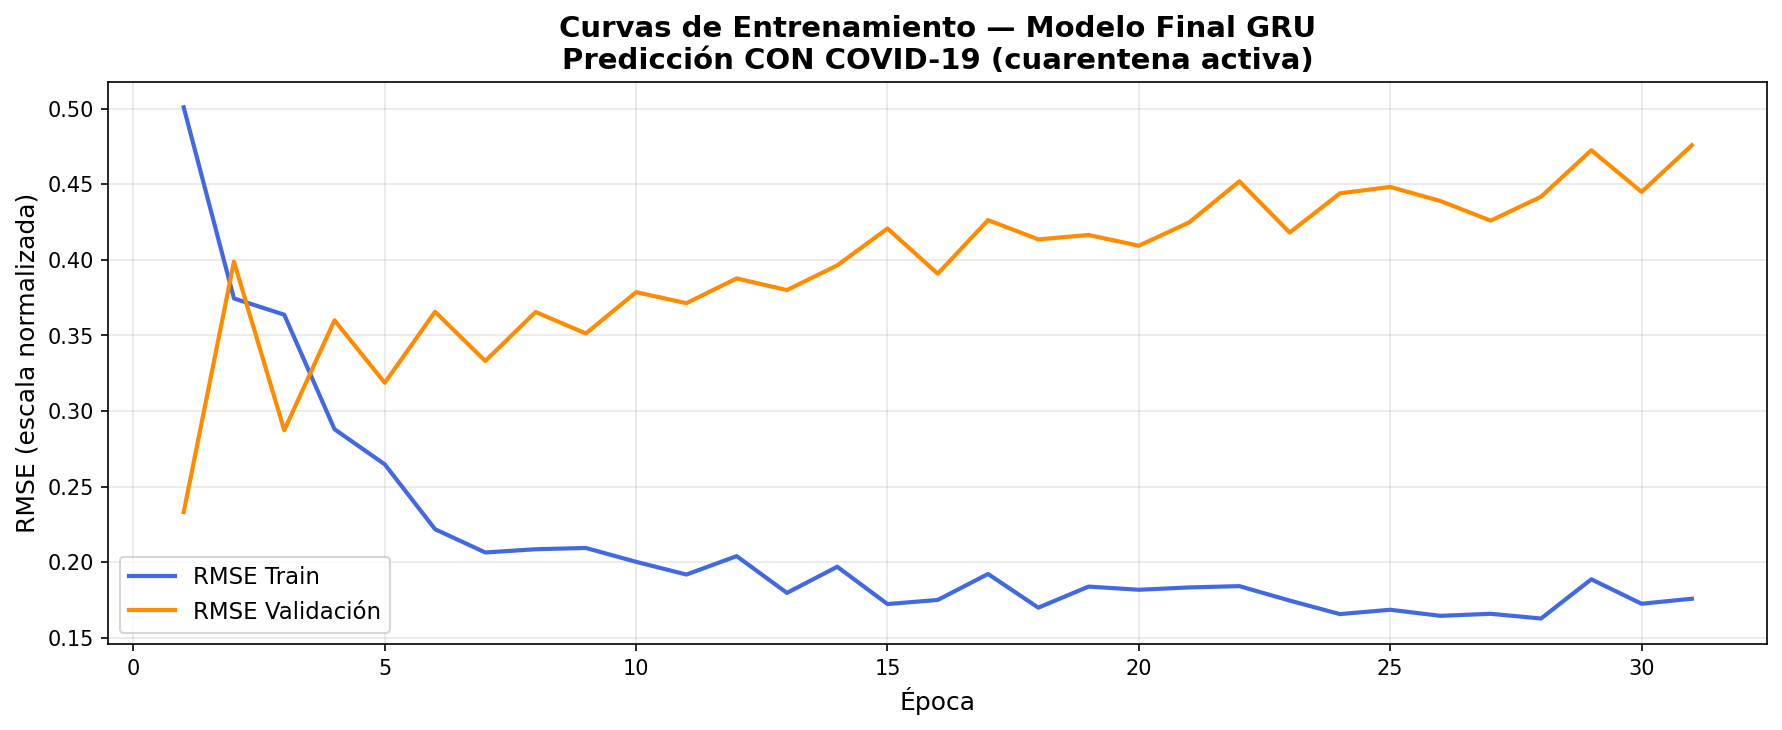
\includegraphics[width=\textwidth]{predicciones/prediccion_cemento_gru/resultados_con_covid/final_01_curvas_entrenamiento.png}
    \caption{Curvas de aprendizaje del modelo GRU para cemento --- escenario con pandemia.}
    \label{fig:gru_cemento_curva_cc}
\end{figure}

\paragraph{Métricas de Evaluación}

\begin{table}[htbp]
    \centering
    \caption{Desempeño del modelo GRU para cemento --- escenario con pandemia: RMSE en train, val y test.}
    \label{tab:gru_cemento_cc_metricas}
    \begin{tabular}{lrrr}
        \toprule
        \textbf{Métrica} & \textbf{Train} & \textbf{Val} & \textbf{Test} \\
        \midrule
        RMSE (Gs.) & 5.343{,}63 & 4.130{,}82 & 1.694{,}23 \\
        \bottomrule
    \end{tabular}
\end{table}

\justify
El RMSE de prueba para el escenario con pandemia (Gs.~1.694{,}23) resulta notablemente inferior al obtenido en el escenario sin pandemia (Gs.~2.709{,}13), lo que indica que la inclusión de la variable pandémica en el entrenamiento mejora el ajuste del modelo sobre el período de evaluación. Sin embargo, el RMSE de entrenamiento (Gs.~5.343{,}63) es más elevado que en el escenario sin pandemia (Gs.~4.911{,}67), lo que puede atribuirse a la mayor variabilidad introducida por los datos pandémicos en el conjunto de entrenamiento.

\paragraph{Evaluación sobre el Conjunto de Prueba}

\begin{figure}[htbp]
    \centering
    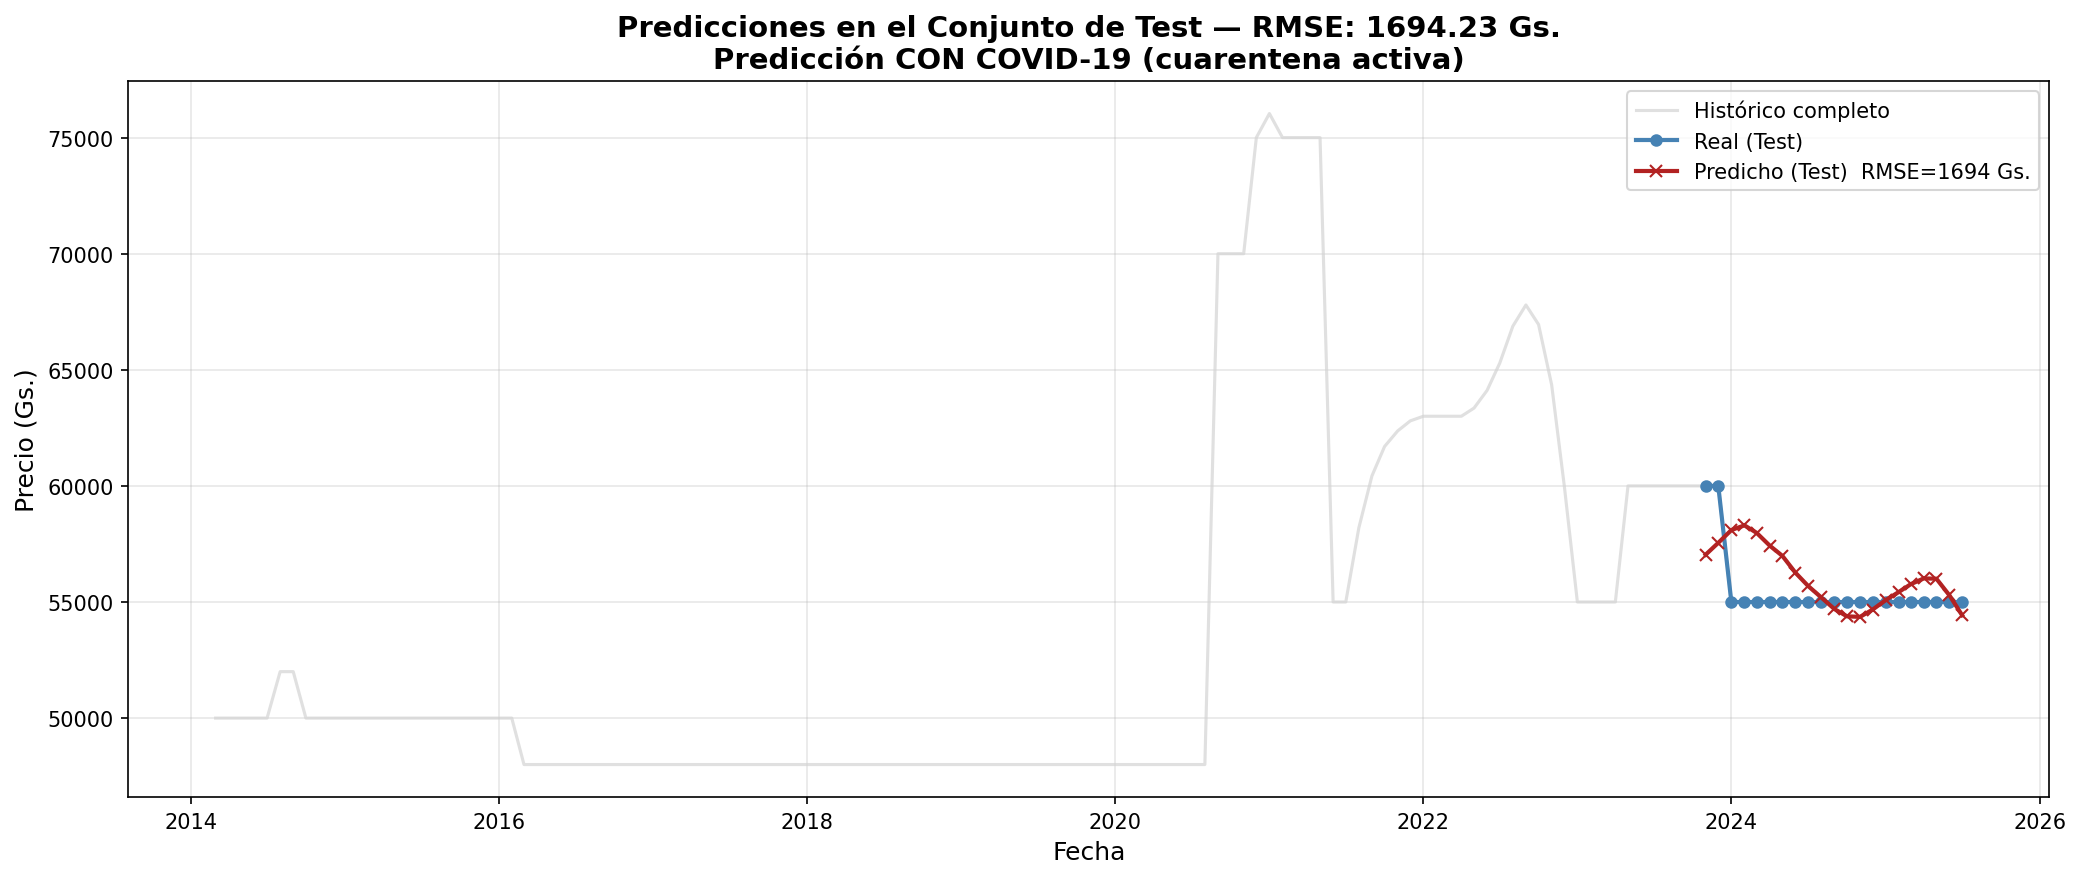
\includegraphics[width=\textwidth]{predicciones/prediccion_cemento_gru/resultados_con_covid/final_02_prediccion_test_serie.png}
    \caption{Predicción GRU vs.\ valores reales del precio del cemento --- escenario con pandemia, conjunto de prueba.}
    \label{fig:gru_cemento_test_cc}
\end{figure}

\begin{figure}[htbp]
    \centering
    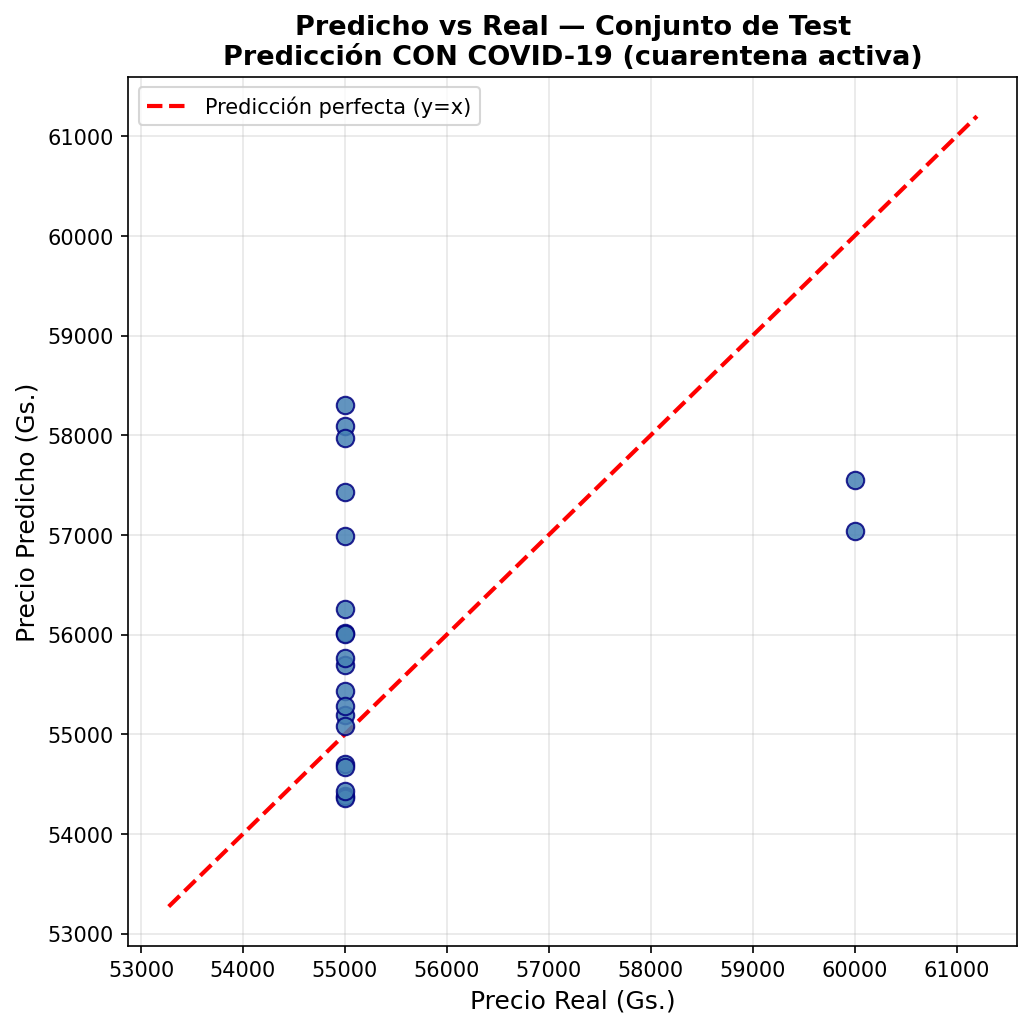
\includegraphics[width=0.8\textwidth]{predicciones/prediccion_cemento_gru/resultados_con_covid/final_03_scatter_test.png}
    \caption{Diagrama de dispersión: precio predicho vs.\ real del cemento --- escenario con pandemia (GRU).}
    \label{fig:gru_cemento_scatter_cc}
\end{figure}

\begin{figure}[htbp]
    \centering
    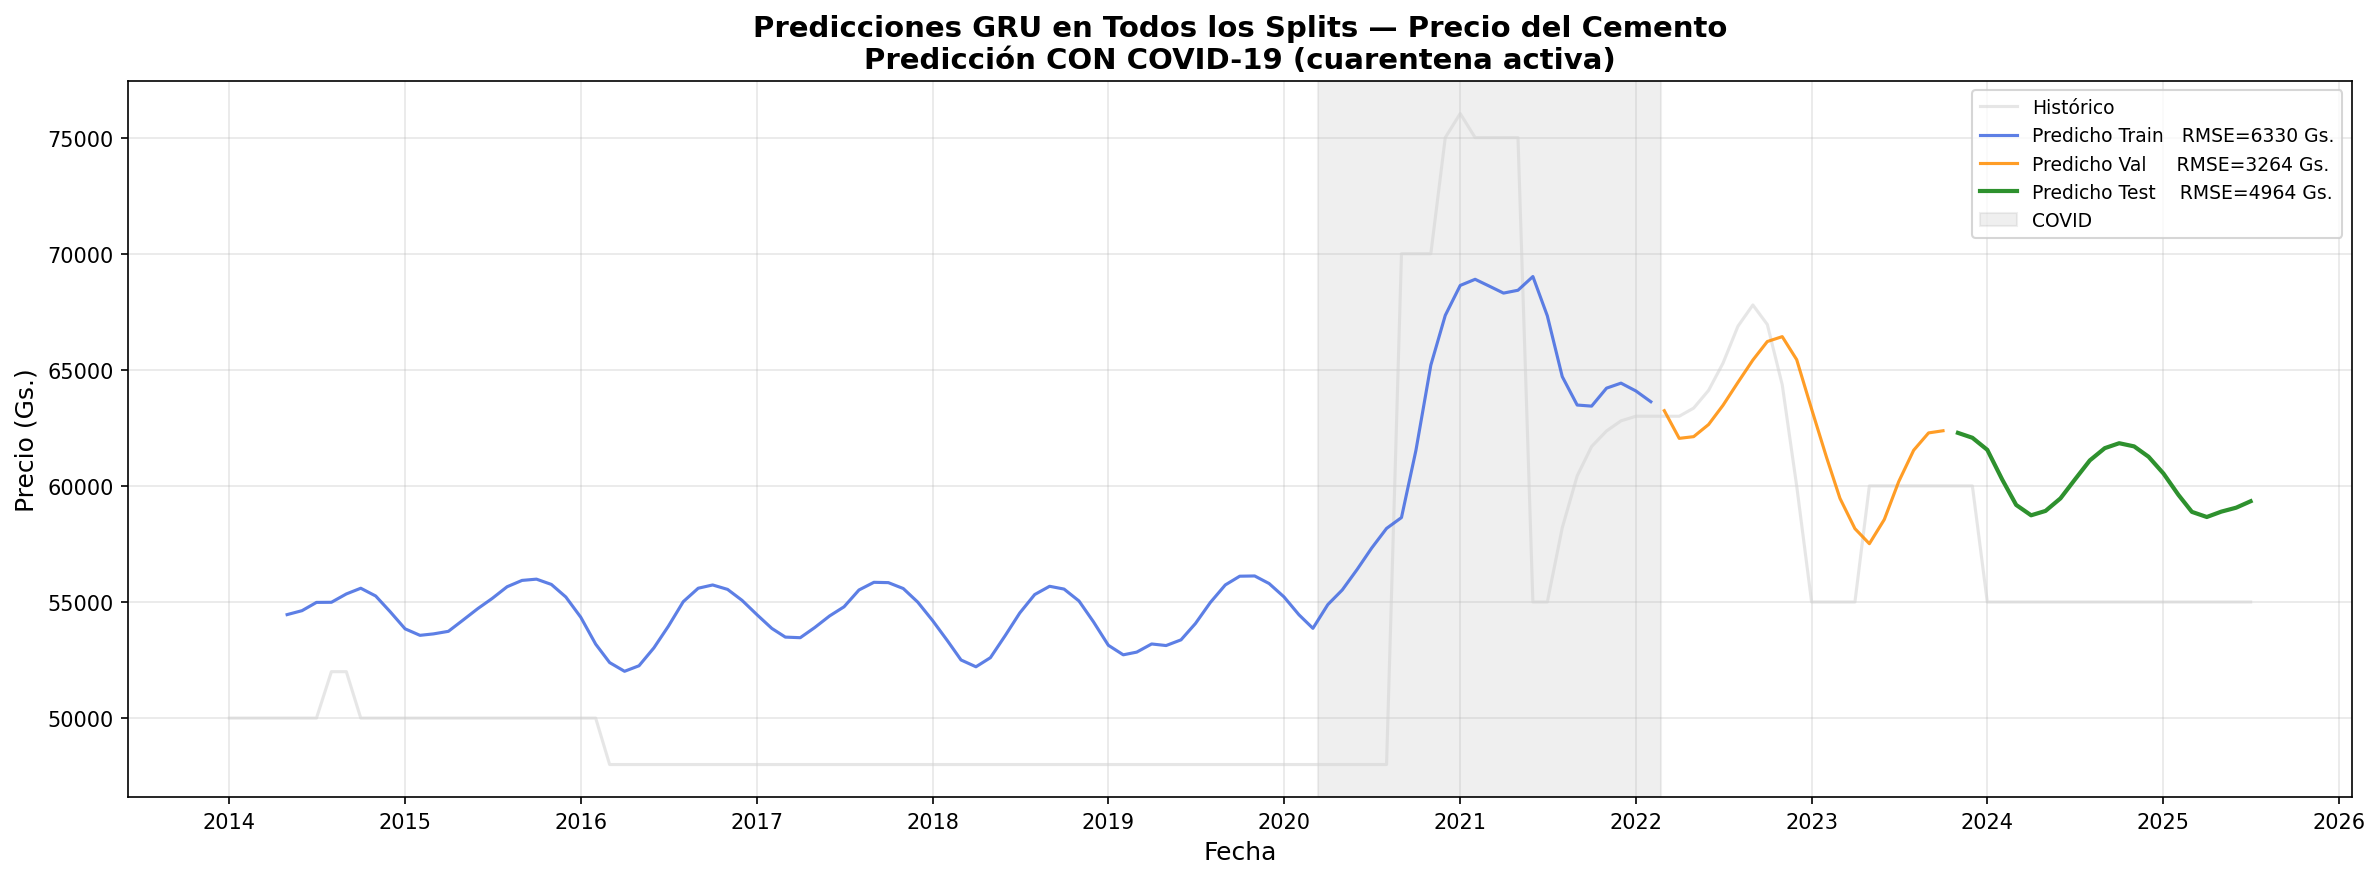
\includegraphics[width=\textwidth]{predicciones/prediccion_cemento_gru/resultados_con_covid/final_05_todos_splits.png}
    \caption{Ajuste del modelo GRU del cemento sobre las tres particiones --- escenario con pandemia.}
    \label{fig:gru_cemento_splits_cc}
\end{figure}

\clearpage
\paragraph{Análisis de Residuos}

\begin{figure}[htbp]
    \centering
    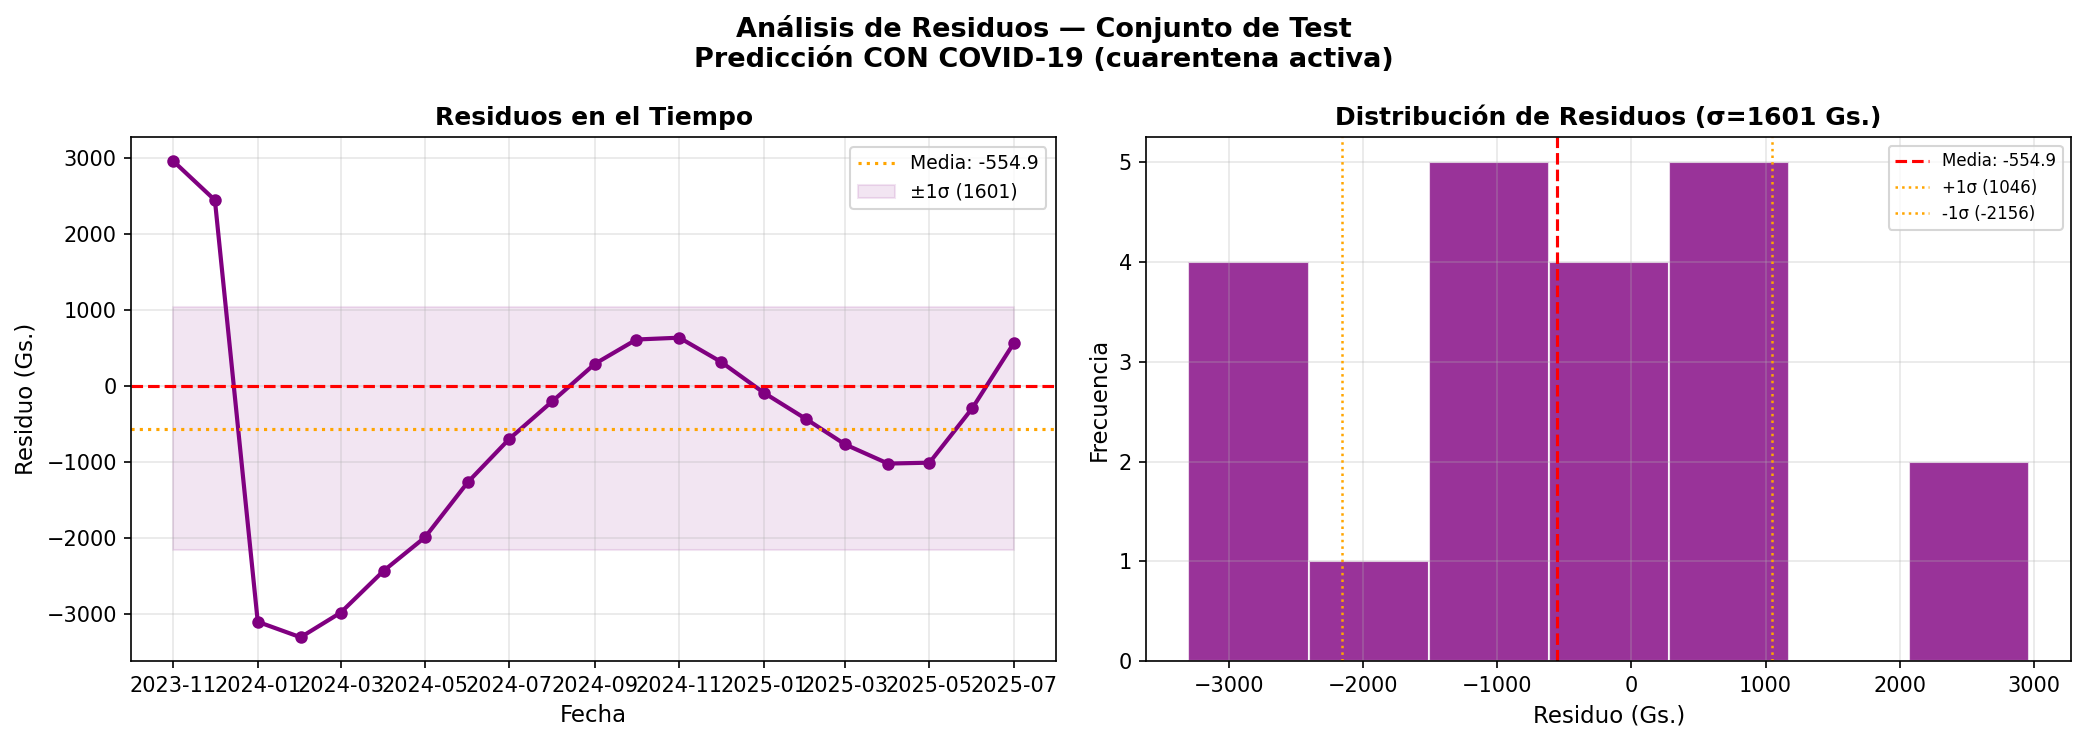
\includegraphics[width=\textwidth]{predicciones/prediccion_cemento_gru/resultados_con_covid/final_04_residuos.png}
    \caption{Residuos del modelo GRU para cemento --- escenario con pandemia, conjunto de prueba.}
    \label{fig:gru_cemento_res_cc}
\end{figure}

\begin{figure}[htbp]
    \centering
    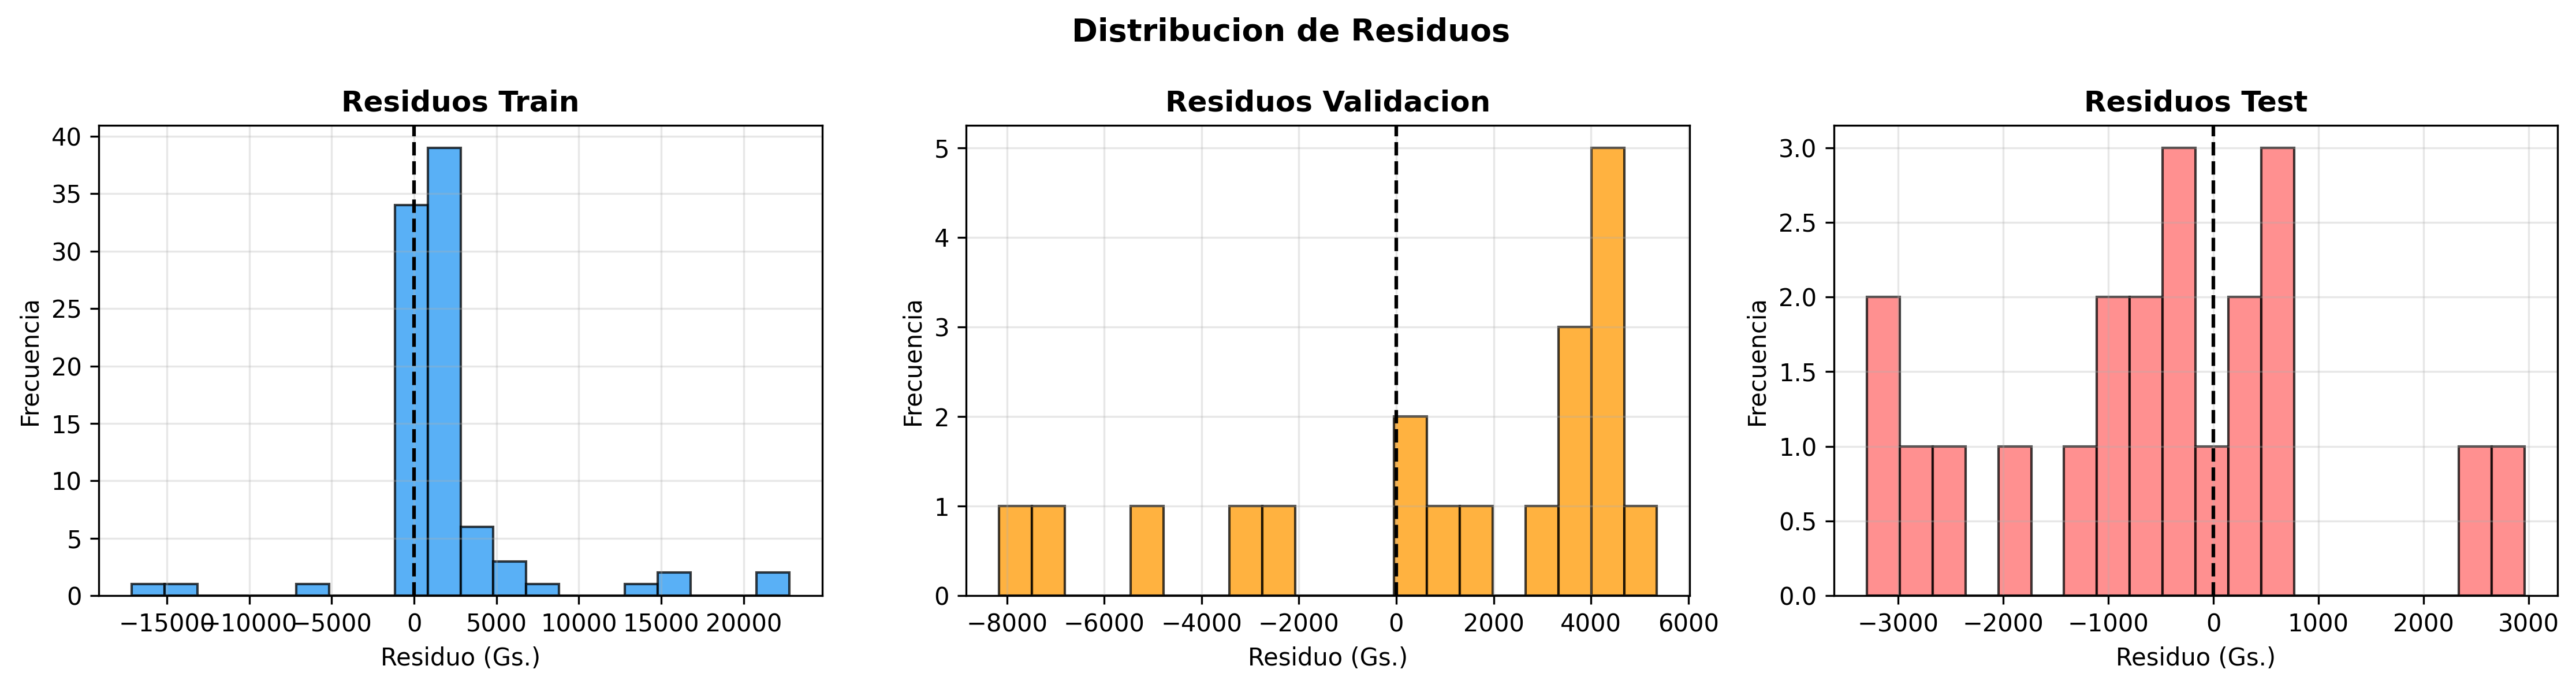
\includegraphics[width=0.8\textwidth]{predicciones/prediccion_cemento_gru/resultados_con_covid/residuos_histograma.png}
    \caption{Histograma de residuos del modelo GRU para cemento --- escenario con pandemia.}
    \label{fig:gru_cemento_reshist_cc}
\end{figure}

\begin{figure}[htbp]
    \centering
    \includegraphics[width=\textwidth]{predicciones/prediccion_cemento_gru/resultados_con_covid/residuos_acf_pacf.png}
    \caption{ACF y PACF de los residuos del modelo GRU para cemento --- escenario con pandemia.}
    \label{fig:gru_cemento_acf_cc}
\end{figure}

\justify
El test de Ljung-Box sobre los residuos del conjunto de prueba arroja un $p$-valor de 0,080 a 10 rezagos y de 0,151 a 20 rezagos, ambos superiores al umbral de 0,05. Esto confirma que los residuos del modelo GRU del cemento bajo el escenario con pandemia se comportan como ruido blanco, resultado más favorable que el obtenido en el escenario sin pandemia (donde existía autocorrelación a 10 rezagos). La inclusión de la variable pandémica parece haber reducido la autocorrelación residual, posiblemente al absorber parte de la estructura temporal que el modelo sin ese indicador no podía explicar.

\clearpage
\paragraph{Pronóstico a 24 Meses}

\begin{figure}[htbp]
    \centering
    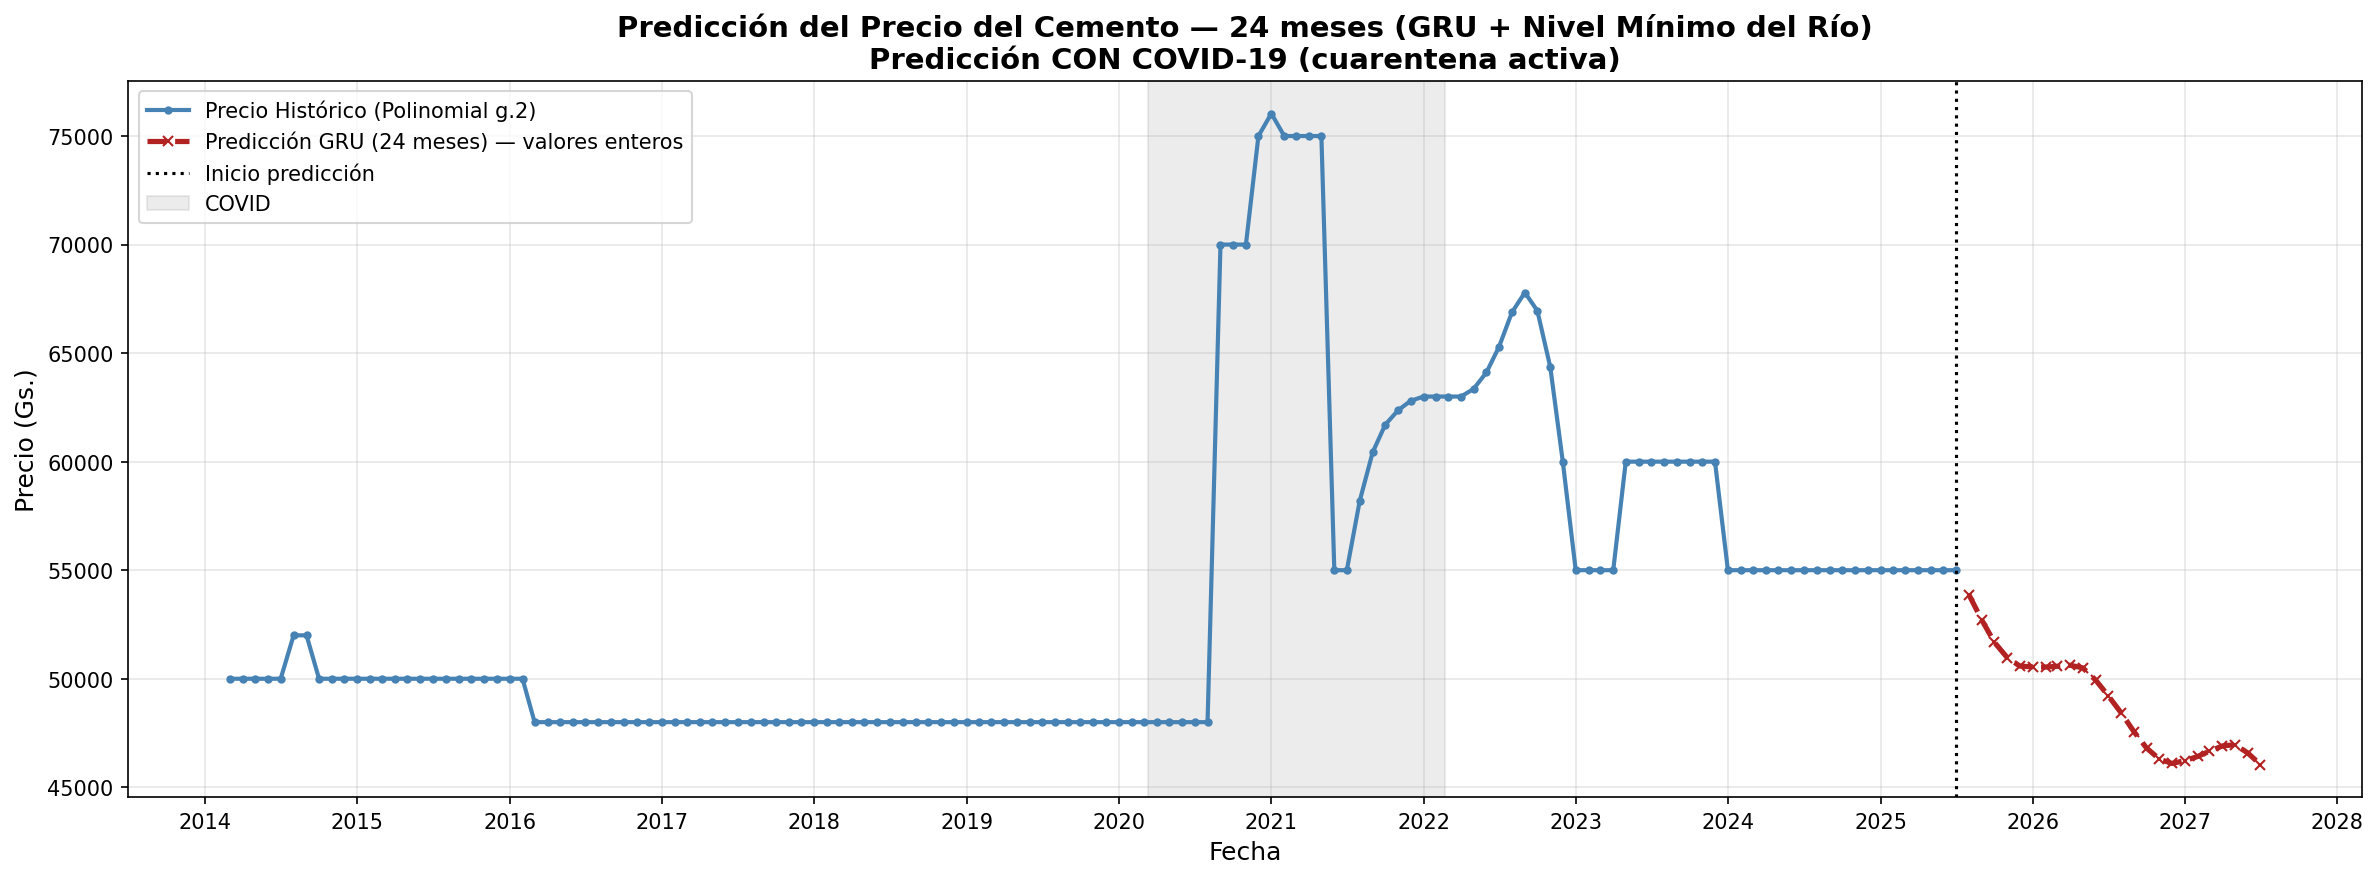
\includegraphics[width=\textwidth]{predicciones/prediccion_cemento_gru/resultados_con_covid/final_06_prediccion_futura_completa.png}
    \caption{Pronóstico GRU del precio del cemento a 24 meses --- escenario con pandemia: serie histórica y proyección.}
    \label{fig:gru_cemento_pred_con_covid}
\end{figure}

\begin{figure}[htbp]
    \centering
    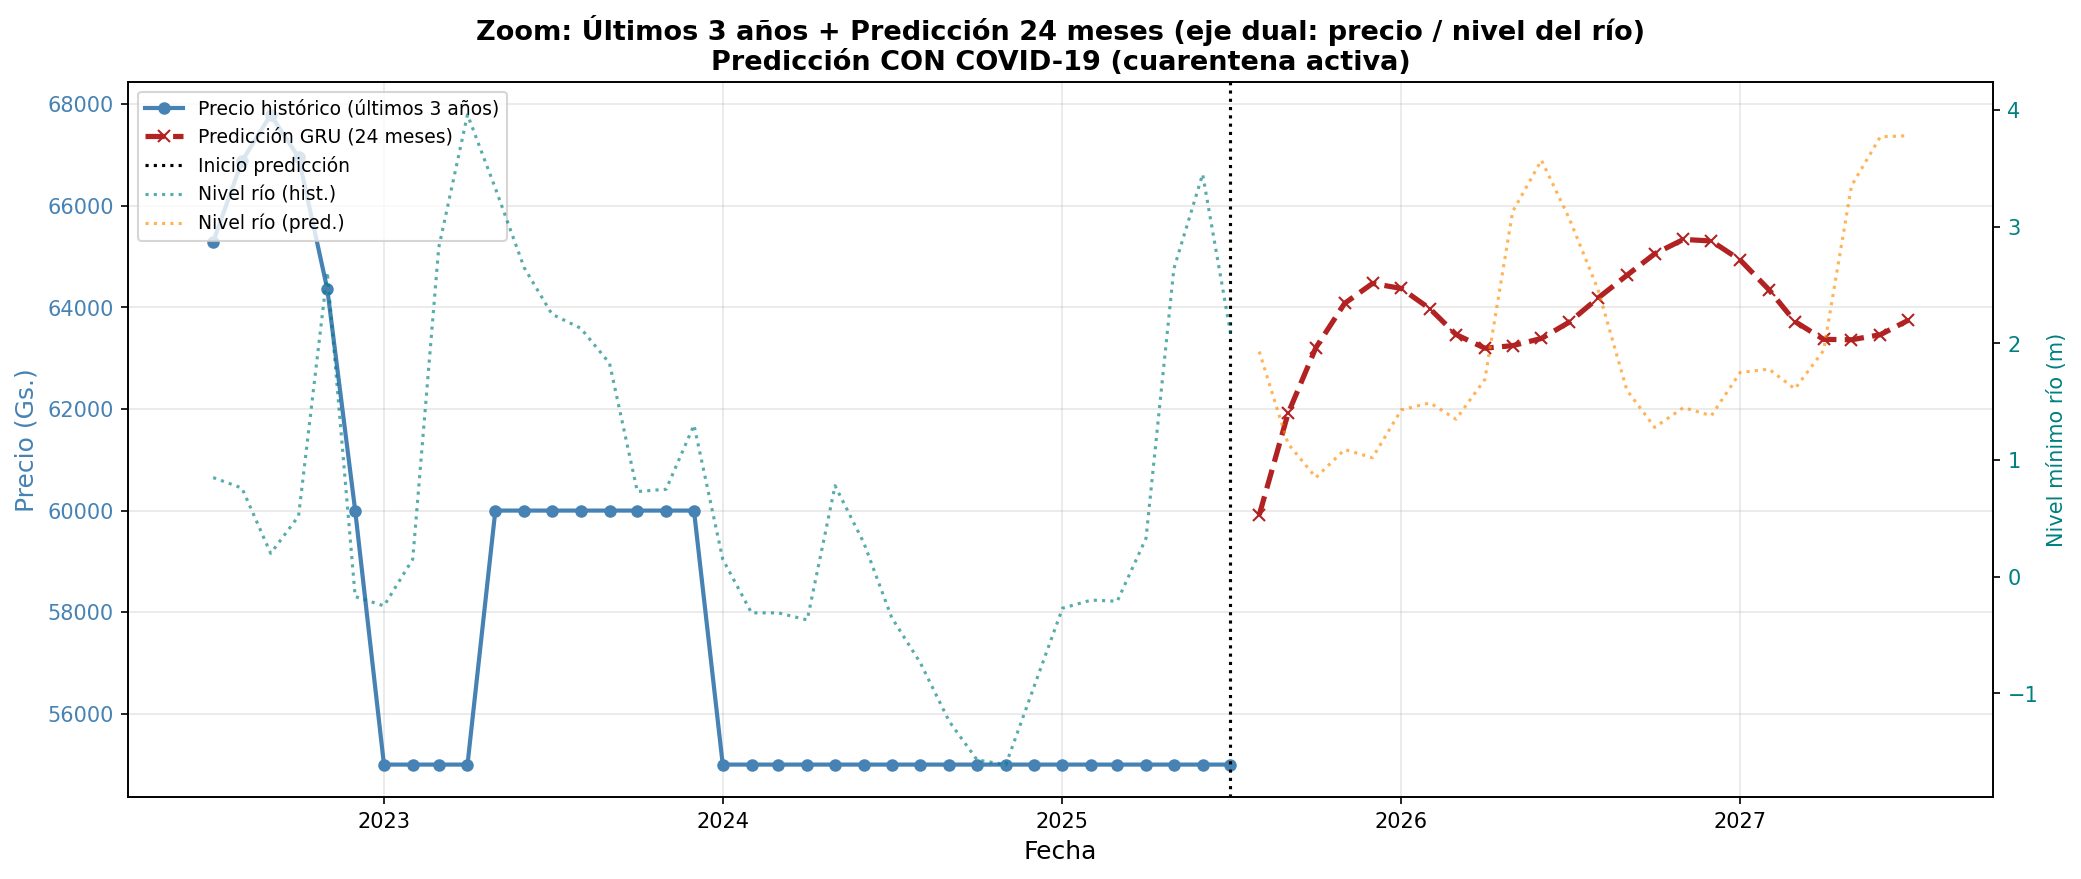
\includegraphics[width=\textwidth]{predicciones/prediccion_cemento_gru/resultados_con_covid/final_07_prediccion_zoom_dual.png}
    \caption{Zoom sobre la transición entre datos observados y pronóstico GRU del cemento --- escenario con pandemia.}
    \label{fig:gru_cemento_zoom_con_covid}
\end{figure}

\begin{figure}[htbp]
    \centering
    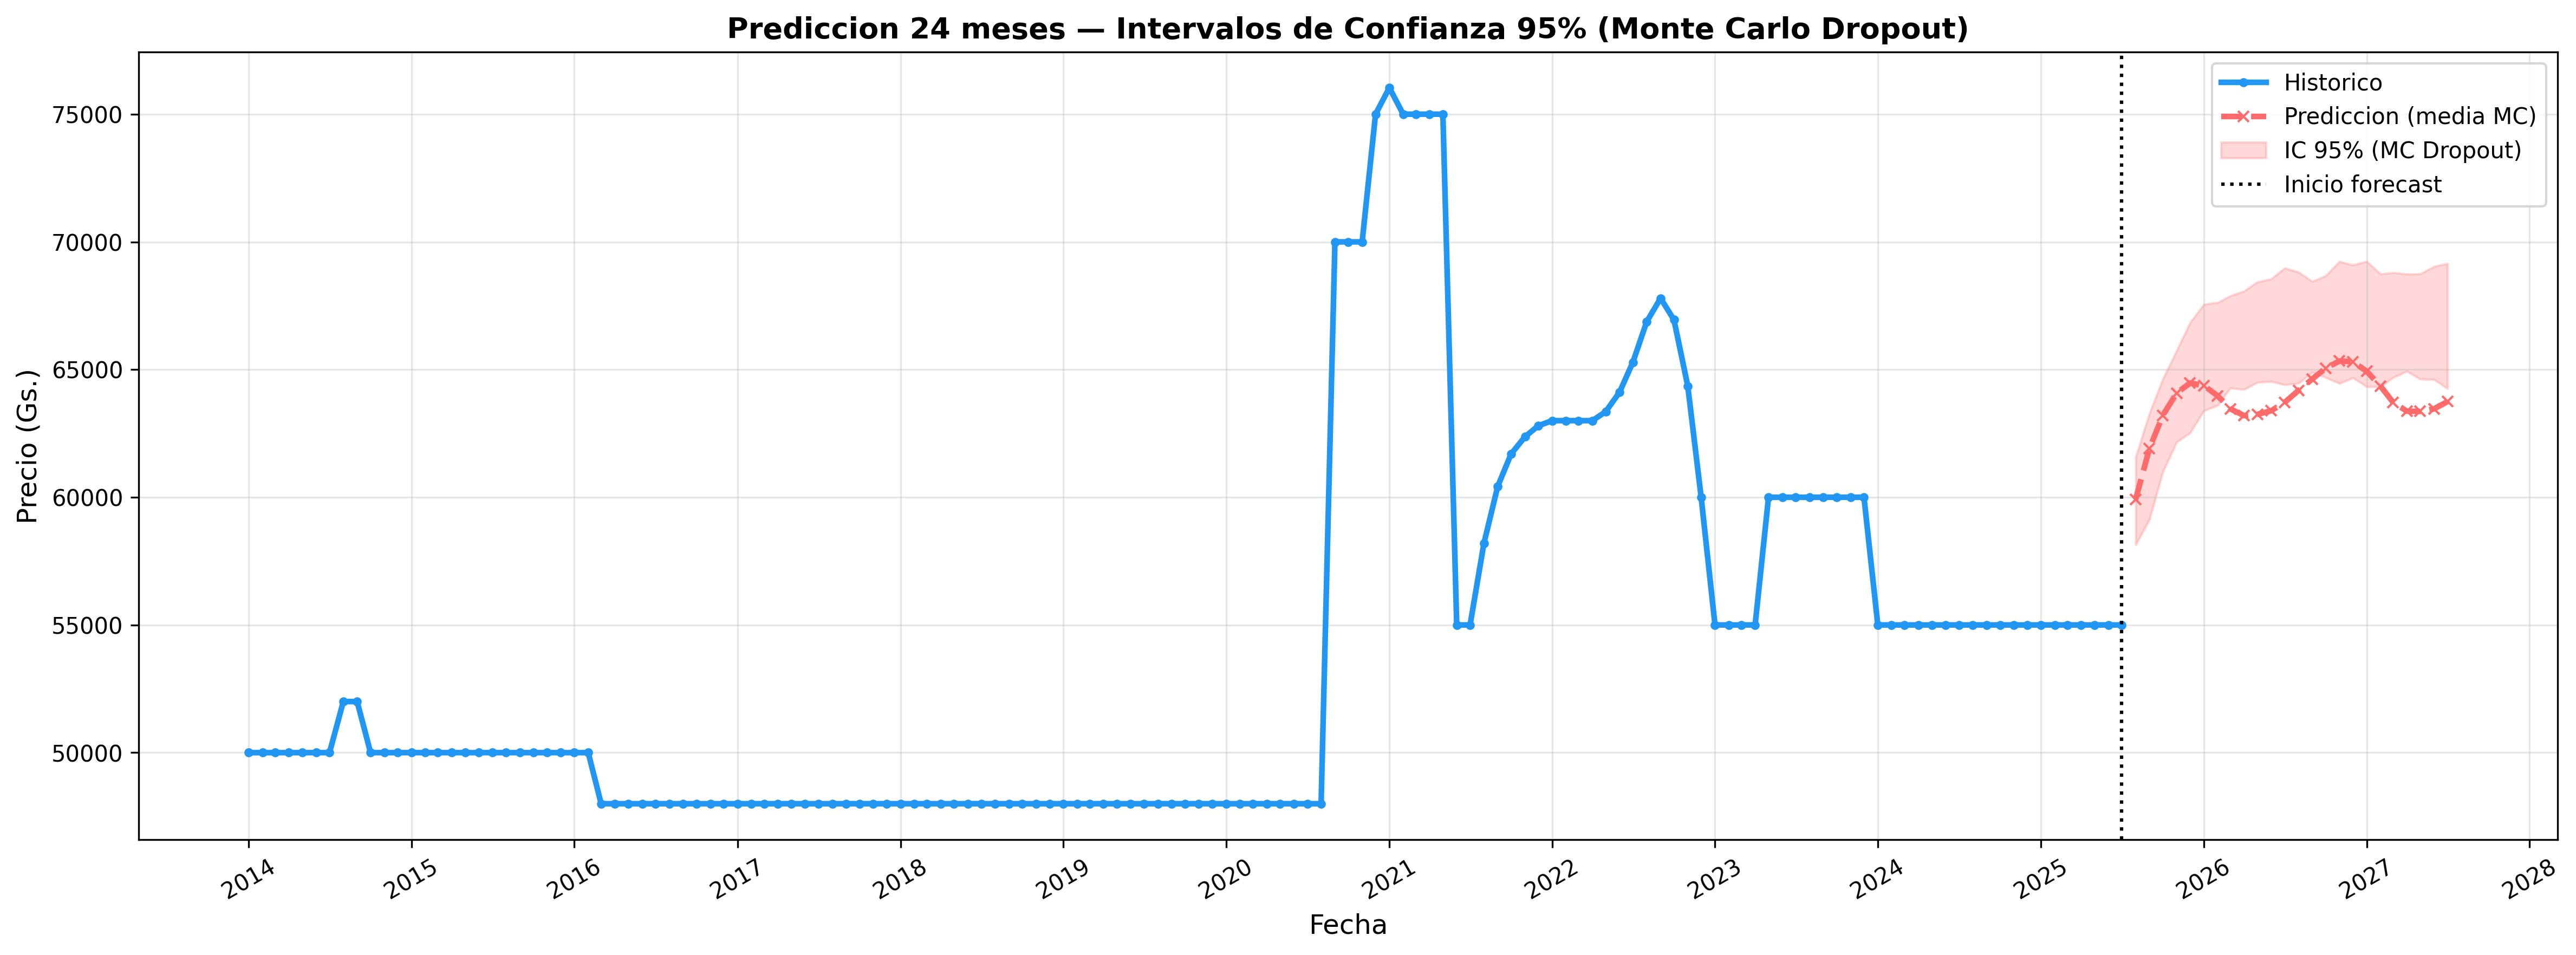
\includegraphics[width=\textwidth]{predicciones/prediccion_cemento_gru/resultados_con_covid/forecast_ic_monte_carlo.png}
    \caption{IC Monte Carlo Dropout del pronóstico GRU para cemento --- escenario con pandemia.}
    \label{fig:gru_cemento_ic_con_covid}
\end{figure}

\justify
Bajo el escenario con efecto pandémico, el modelo GRU proyecta para el cemento precios considerablemente inferiores al escenario sin pandemia, con el rango completo entre Gs.~46.048 y Gs.~53.874. La diferencia es sustancial: mientras que sin pandemia el precio asciende hasta Gs.~61.845, con pandemia el modelo proyecta una trayectoria descendente que alcanza un mínimo de Gs.~46.048. La GRU interpreta la señal de cuarentena activa como un factor de contracción de la demanda, lo que contrasta con la interpretación alcista que el LSTM asignó al mismo escenario. Este resultado es un hallazgo relevante de la comparación entre arquitecturas: ambas redes aprendieron aspectos diferentes del fenómeno pandémico a partir de los mismos datos históricos.

% ============================================================
% 4.4.2 — LADRILLO GRU
% ============================================================
\clearpage
\subsection{Predicción del Precio del Ladrillo}

\justify
Para el ladrillo, la búsqueda con Optuna fue realizada de forma independiente en cada escenario y ambos convergieron a la misma configuración GRU unidireccional con 64 unidades ocultas y 13.889 parámetros entrenables. A continuación se presenta cada escenario por separado.

% ------ LADRILLO GRU SIN COVID ------
\clearpage
\subsubsection{Escenario sin Efecto Pandémico}

\paragraph{Hiperparámetros y Arquitectura}

\justify
La búsqueda con Optuna (261 ensayos, 194,9 min) identificó una arquitectura GRU unidireccional con 64 unidades ocultas y ventana de entrada (\textit{lookback}) de 3 meses. El optimizador Adam con $\eta = 0{,}008441$ y \textit{weight decay} de $1{,}04 \times 10^{-6}$ resultó la configuración más eficiente, junto con \textit{batch size} de 8, \textit{dropout} de 0{,}05, \textit{dropout} recurrente de 0{,}2 y \textit{scheduler} StepLR. La arquitectura totaliza 13.889 parámetros entrenables. La Tabla~\ref{tab:gru_ladrillo_sc_arq} resume los hiperparámetros.

\begin{table}[htbp]
    \centering
    \caption{Hiperparámetros del modelo GRU para ladrillo --- escenario sin pandemia (Optuna: 261 ensayos, 194{,}9 min).}
    \label{tab:gru_ladrillo_sc_arq}
    \begin{tabular}{ll}
        \toprule
        \textbf{Hiperparámetro} & \textbf{Valor} \\
        \midrule
        Capas GRU              & 1 (unidireccional) \\
        Unidades ocultas       & 64 \\
        Lookback               & 3 meses \\
        Optimizador            & Adam ($\eta=0{,}008441$, WD $=1{,}04 \times 10^{-6}$) \\
        Batch size             & 8 \\
        Dropout / Rec.\ dropout & 0{,}05 / 0{,}2 \\
        Scheduler              & StepLR \\
        Parámetros entrenables & 13.889 \\
        \bottomrule
    \end{tabular}
\end{table}

\paragraph{Curva de Aprendizaje}

\justify
El modelo GRU del ladrillo para el escenario sin pandemia convergió en 62 épocas con \textit{early stopping}. La Figura~\ref{fig:gru_ladrillo_curva_sc} muestra las curvas de pérdida. La convergencia en pocas épocas es consistente con la tasa de aprendizaje relativamente alta ($\eta=0{,}008441$) del optimizador Adam, que permite alcanzar rápidamente una región de mínimo local, mientras que el \textit{scheduler} StepLR reduce gradualmente la tasa para afinar el ajuste en las épocas finales.

\begin{figure}[htbp]
    \centering
    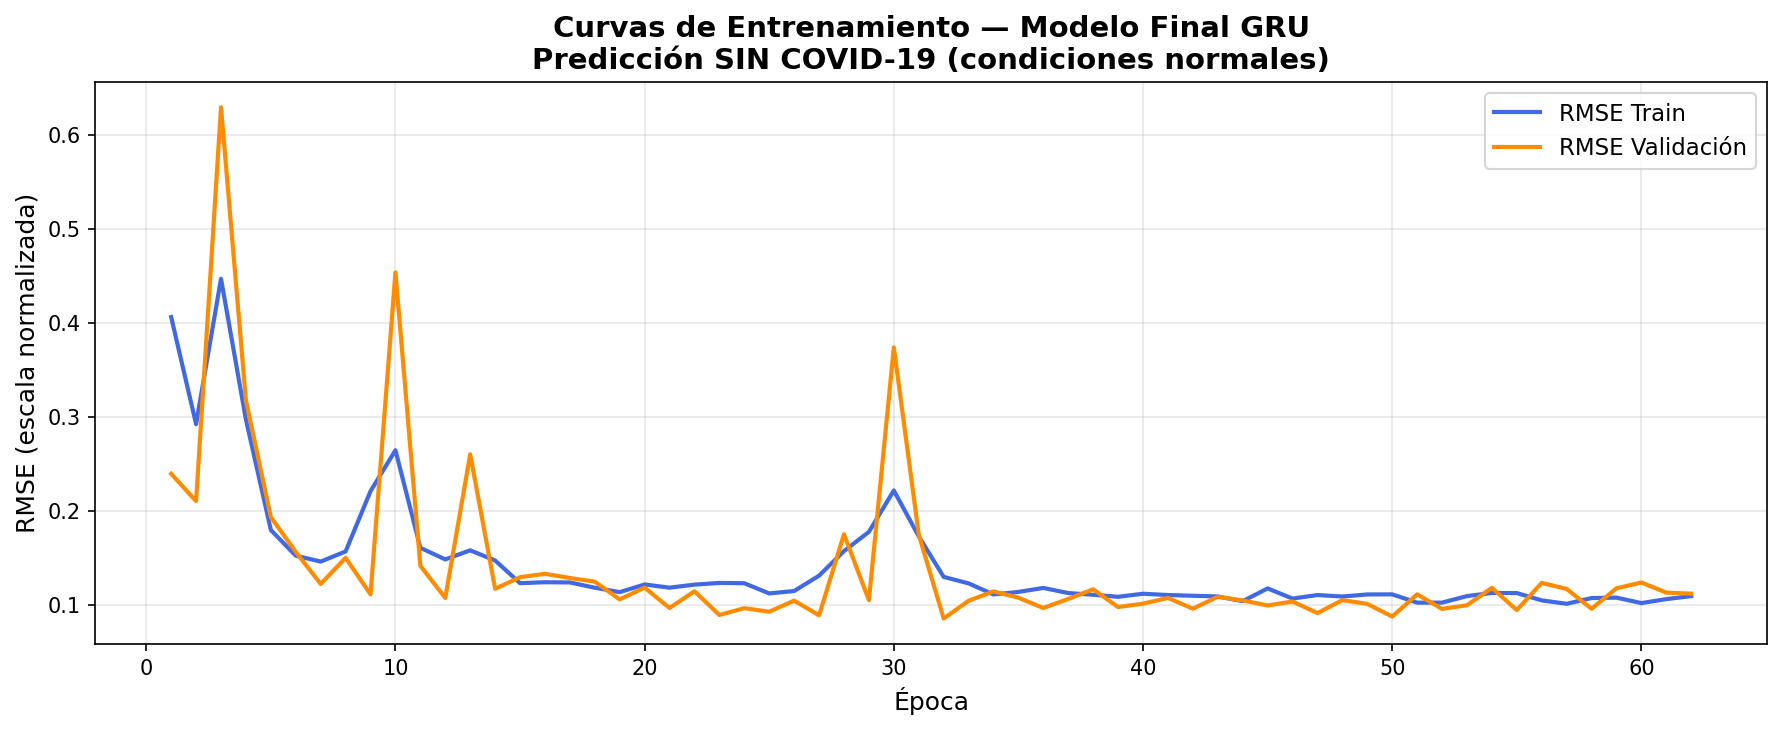
\includegraphics[width=\textwidth]{predicciones/prediccion_ladrillo_gru/resultados_sin_covid/final_01_curvas_entrenamiento.png}
    \caption{Curvas de aprendizaje del modelo GRU para ladrillo --- escenario sin pandemia.}
    \label{fig:gru_ladrillo_curva_sc}
\end{figure}

\paragraph{Métricas de Evaluación}

\begin{table}[htbp]
    \centering
    \caption{Desempeño del modelo GRU para ladrillo --- escenario sin pandemia: RMSE en train, val y test.}
    \label{tab:gru_ladrillo_sc_metricas}
    \begin{tabular}{lrrr}
        \toprule
        \textbf{Métrica} & \textbf{Train} & \textbf{Val} & \textbf{Test} \\
        \midrule
        RMSE (Gs.) & 15{,}56 & 11{,}53 & 11{,}88 \\
        \bottomrule
    \end{tabular}
\end{table}

\justify
El RMSE de validación (Gs.~11{,}53) y el de prueba (Gs.~11{,}88) son coherentes entre sí, lo que indica ausencia de sobreajuste. El RMSE de entrenamiento (Gs.~15{,}56) es mayor porque el período histórico completo de entrenamiento contiene mayor variabilidad que el período de prueba.

\paragraph{Evaluación sobre el Conjunto de Prueba}

\begin{figure}[htbp]
    \centering
    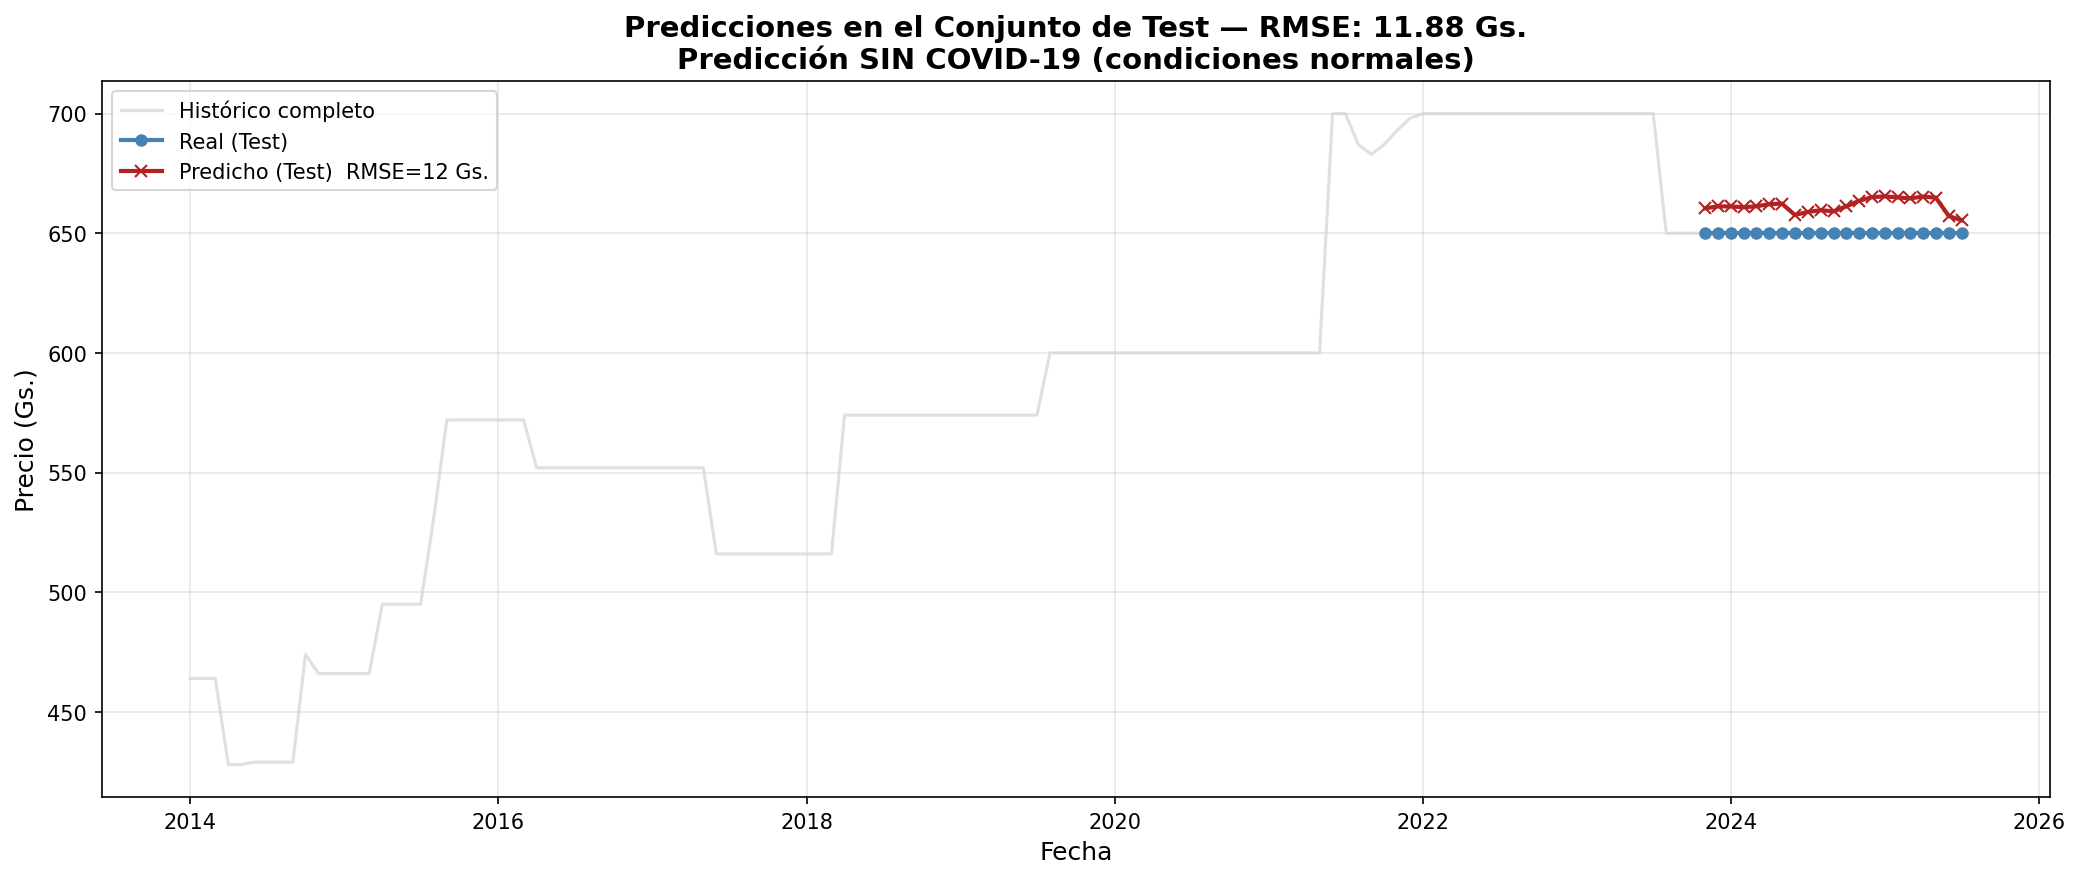
\includegraphics[width=\textwidth]{predicciones/prediccion_ladrillo_gru/resultados_sin_covid/final_02_prediccion_test_serie.png}
    \caption{Predicción GRU vs.\ valores reales del precio del ladrillo --- escenario sin pandemia, conjunto de prueba.}
    \label{fig:gru_ladrillo_test_sc}
\end{figure}

\begin{figure}[htbp]
    \centering
    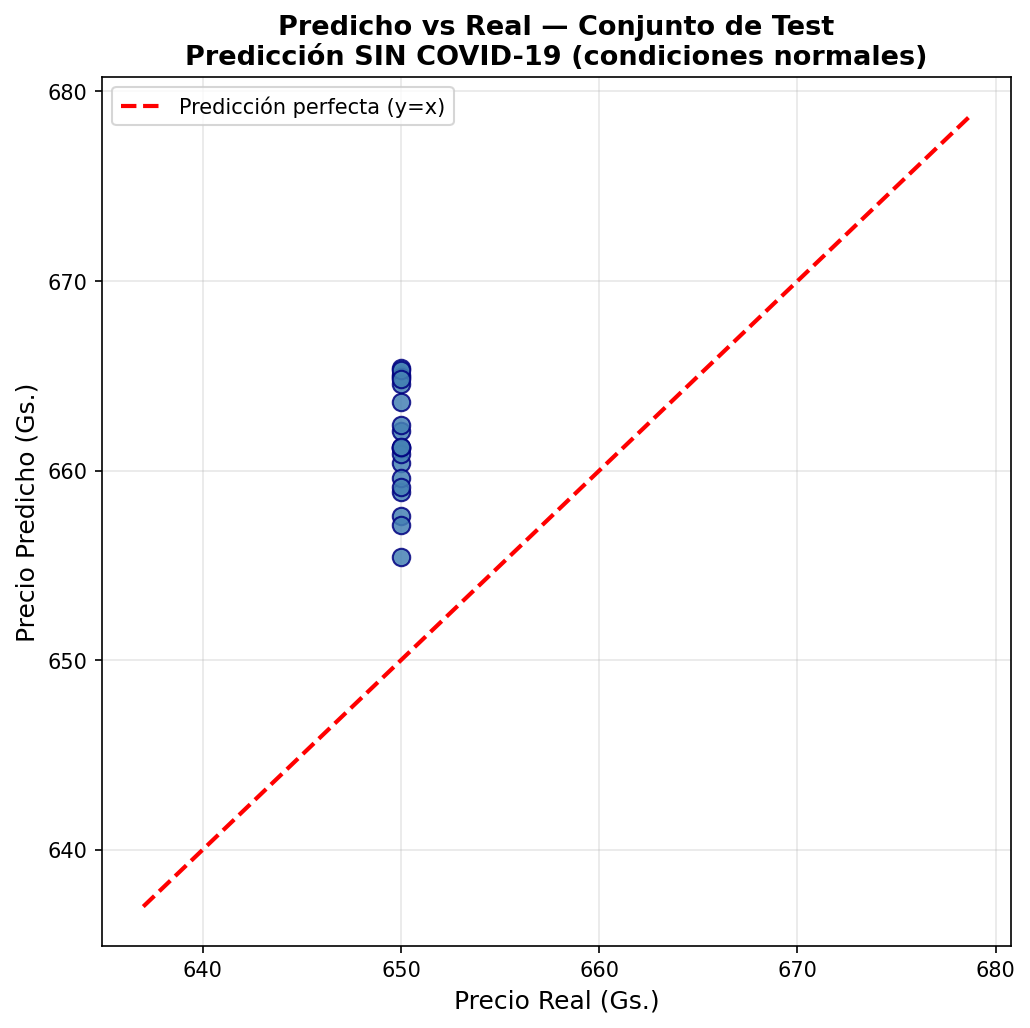
\includegraphics[width=0.8\textwidth]{predicciones/prediccion_ladrillo_gru/resultados_sin_covid/final_03_scatter_test.png}
    \caption{Diagrama de dispersión: precio predicho vs.\ real del ladrillo --- escenario sin pandemia (GRU).}
    \label{fig:gru_ladrillo_scatter_sc}
\end{figure}

\begin{figure}[htbp]
    \centering
    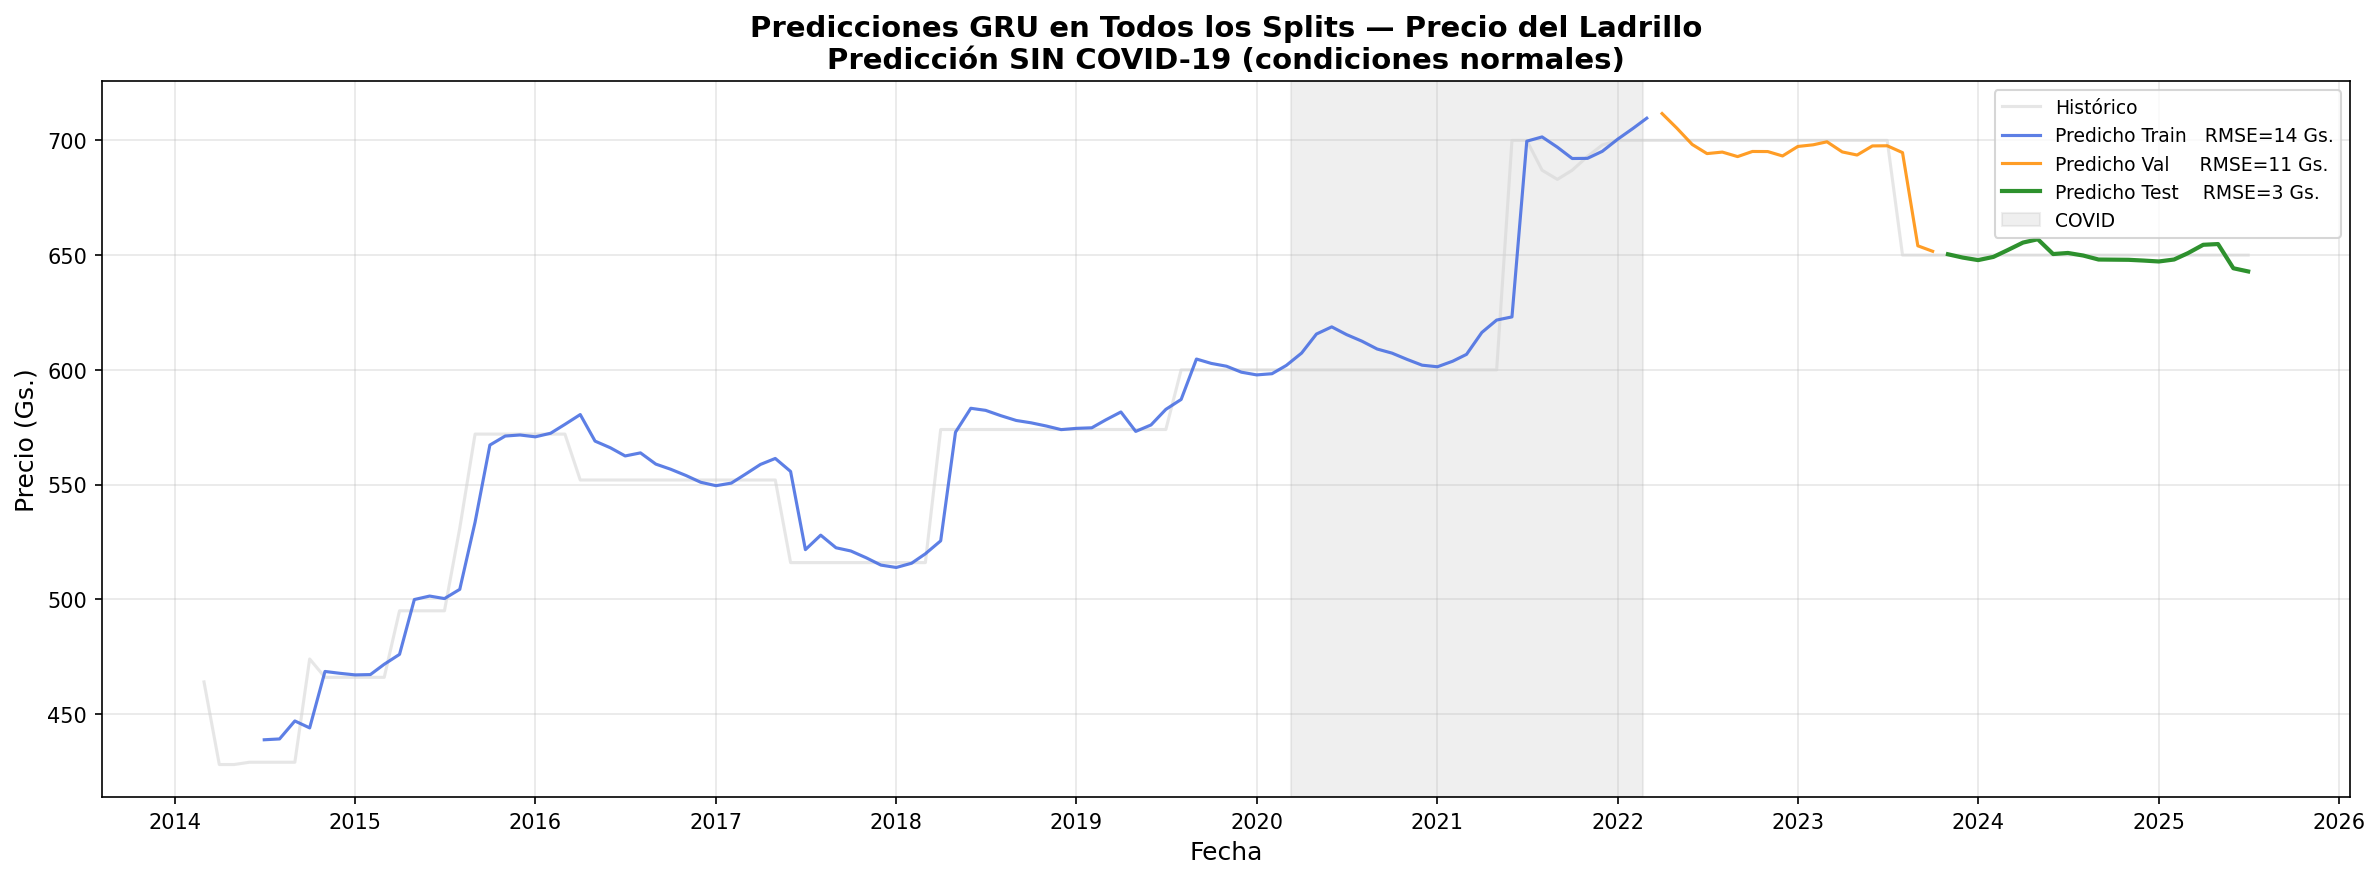
\includegraphics[width=\textwidth]{predicciones/prediccion_ladrillo_gru/resultados_sin_covid/final_05_todos_splits.png}
    \caption{Ajuste del modelo GRU del ladrillo sobre las tres particiones --- escenario sin pandemia.}
    \label{fig:gru_ladrillo_splits_sc}
\end{figure}

\clearpage
\paragraph{Análisis de Residuos}

\begin{figure}[htbp]
    \centering
    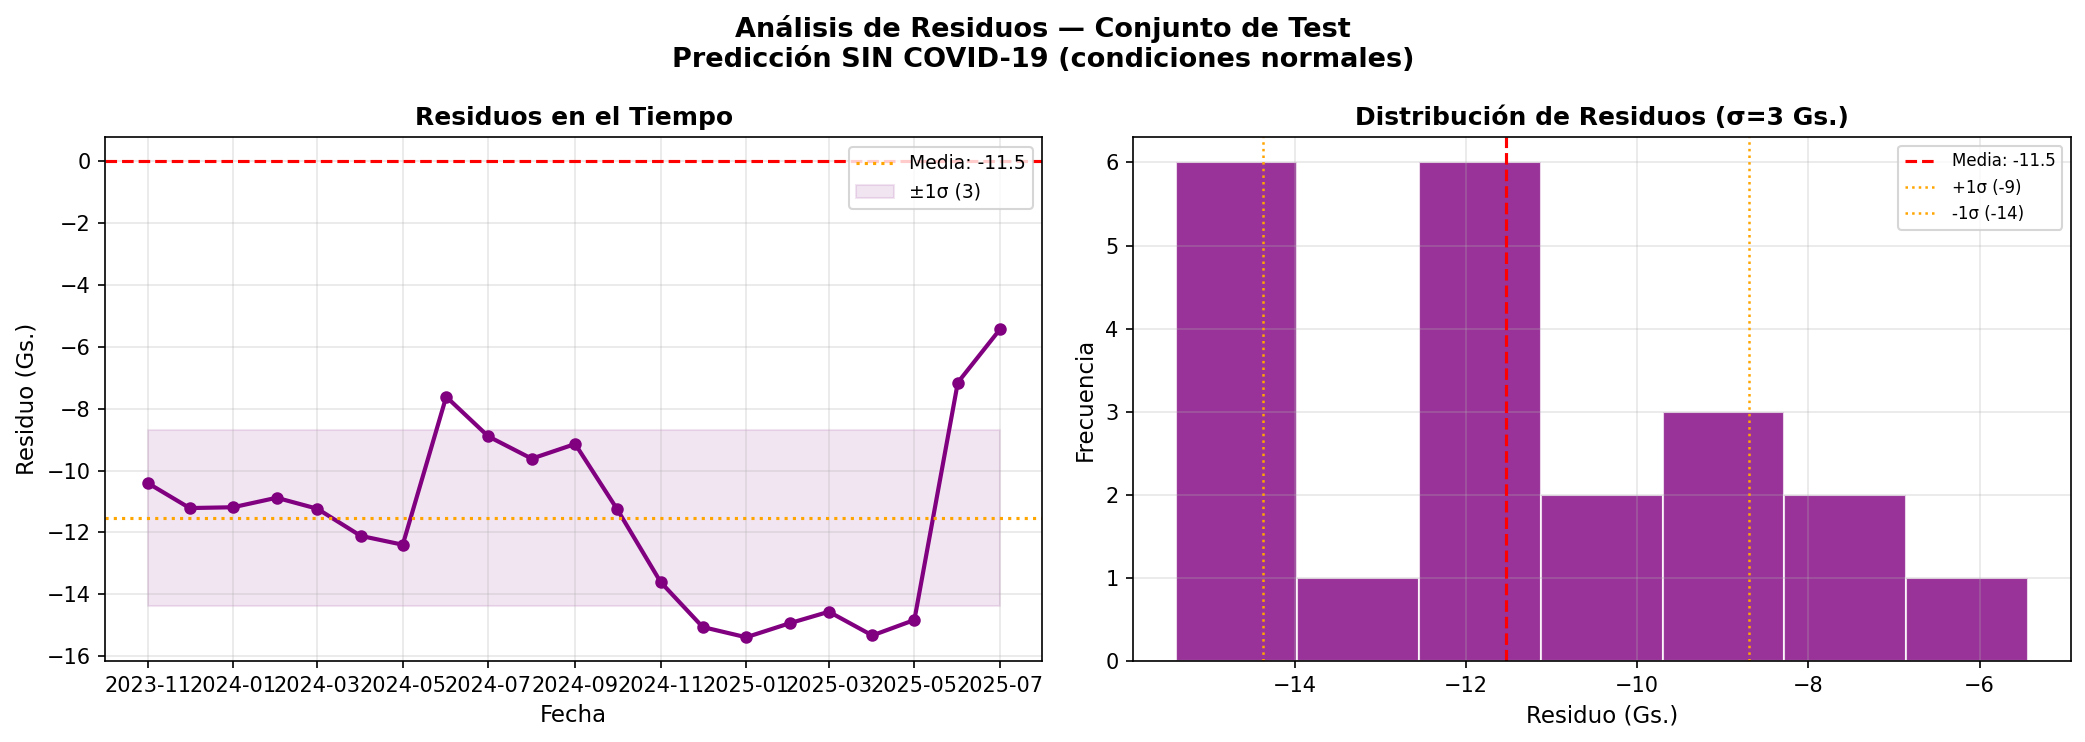
\includegraphics[width=\textwidth]{predicciones/prediccion_ladrillo_gru/resultados_sin_covid/final_04_residuos.png}
    \caption{Residuos del modelo GRU para ladrillo --- escenario sin pandemia, conjunto de prueba.}
    \label{fig:gru_ladrillo_res_sc}
\end{figure}

\begin{figure}[htbp]
    \centering
    \includegraphics[width=0.8\textwidth]{predicciones/prediccion_ladrillo_gru/resultados_sin_covid/residuos_histograma.png}
    \caption{Histograma de residuos del modelo GRU para ladrillo --- escenario sin pandemia.}
    \label{fig:gru_ladrillo_reshist_sc}
\end{figure}

\begin{figure}[htbp]
    \centering
    \includegraphics[width=\textwidth]{predicciones/prediccion_ladrillo_gru/resultados_sin_covid/residuos_acf_pacf.png}
    \caption{ACF y PACF de los residuos del modelo GRU para ladrillo --- escenario sin pandemia.}
    \label{fig:gru_ladrillo_acf_sc}
\end{figure}

\justify
El test de Ljung-Box sobre los residuos del conjunto de prueba no rechaza la hipótesis nula de ausencia de autocorrelación serial en ninguno de los rezagos evaluados: $p=0{,}442$ a 10 rezagos y $p=0{,}081$ a 20 rezagos, ambos superiores al umbral de 0{,}05. Este resultado confirma que los residuos se comportan como ruido blanco y que la estructura temporal de la serie ha sido capturada adecuadamente, un resultado notable para el modelo más compacto del estudio.

\clearpage
\paragraph{Pronóstico a 24 Meses}

\begin{figure}[htbp]
    \centering
    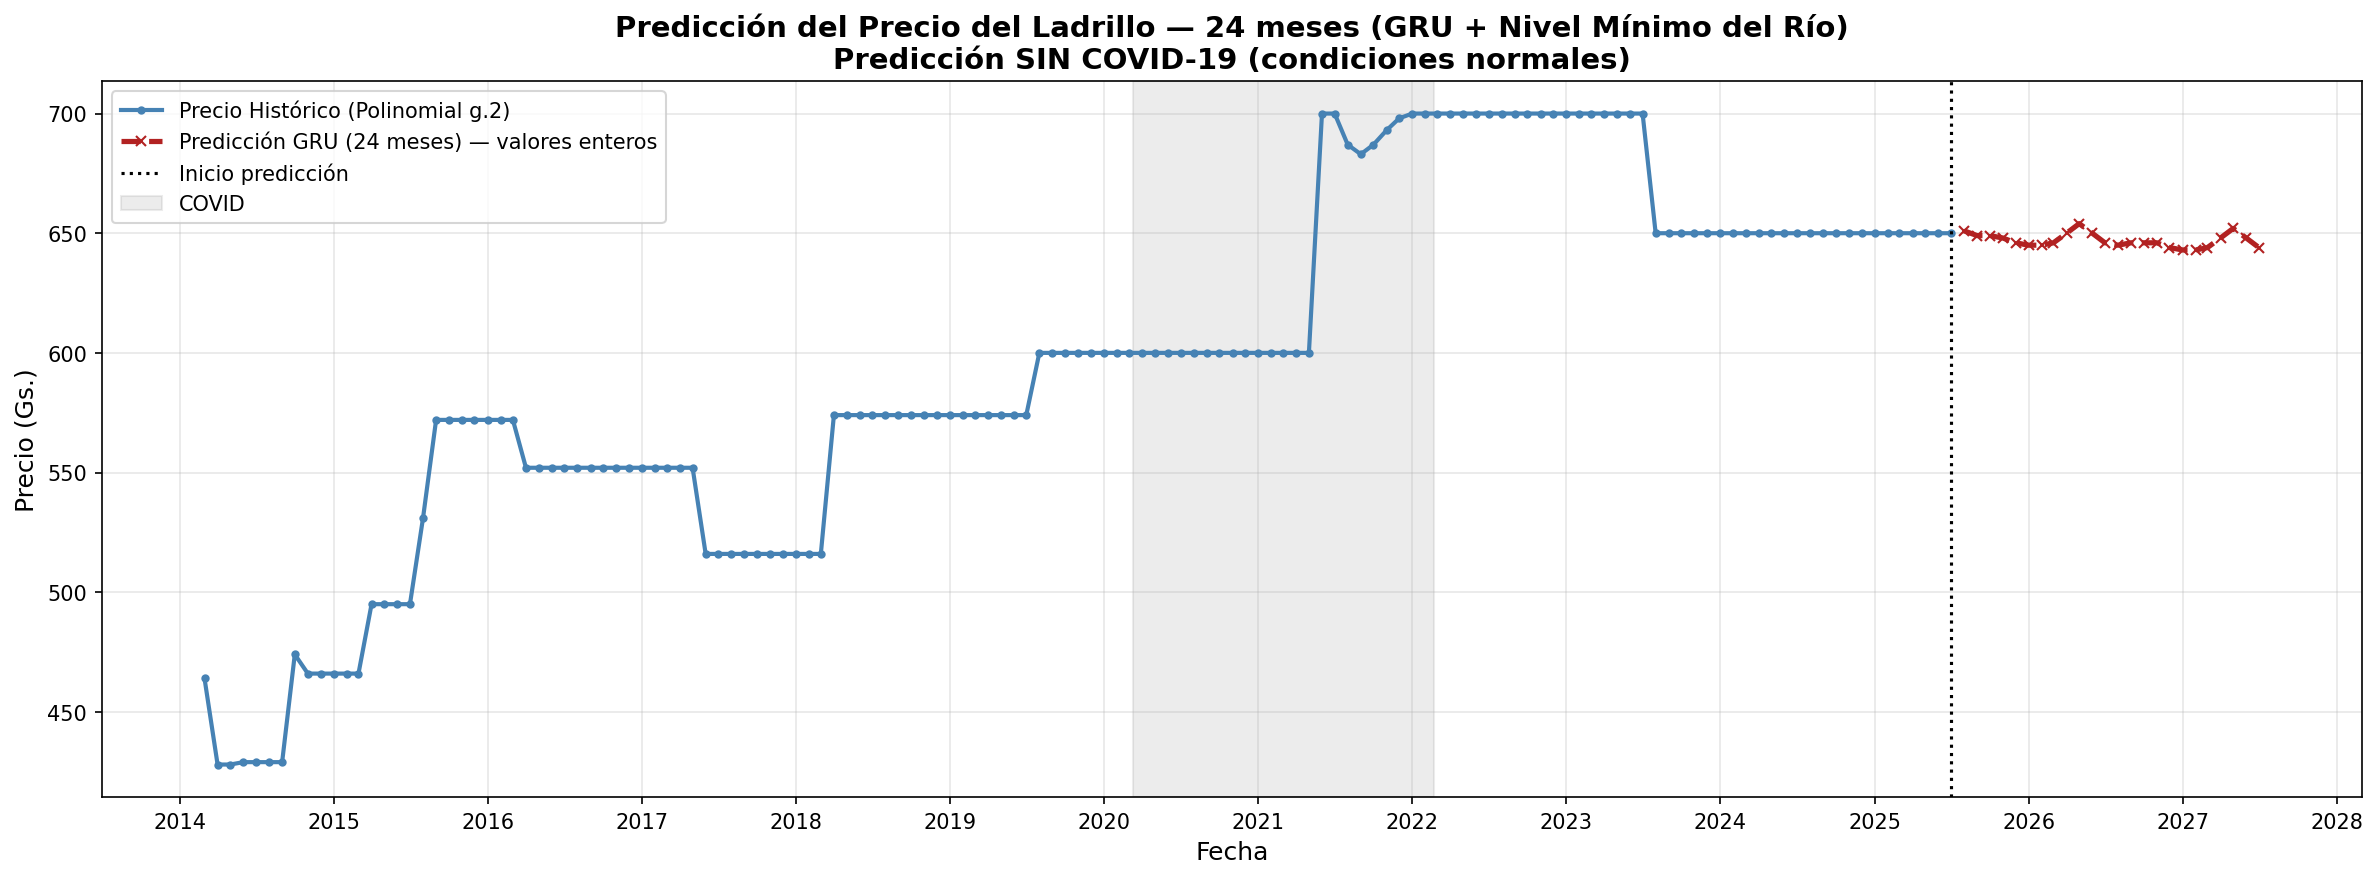
\includegraphics[width=\textwidth]{predicciones/prediccion_ladrillo_gru/resultados_sin_covid/final_06_prediccion_futura_completa.png}
    \caption{Pronóstico GRU del precio del ladrillo a 24 meses --- escenario sin pandemia: serie histórica y proyección.}
    \label{fig:gru_ladrillo_pred_sin_covid}
\end{figure}

\begin{figure}[htbp]
    \centering
    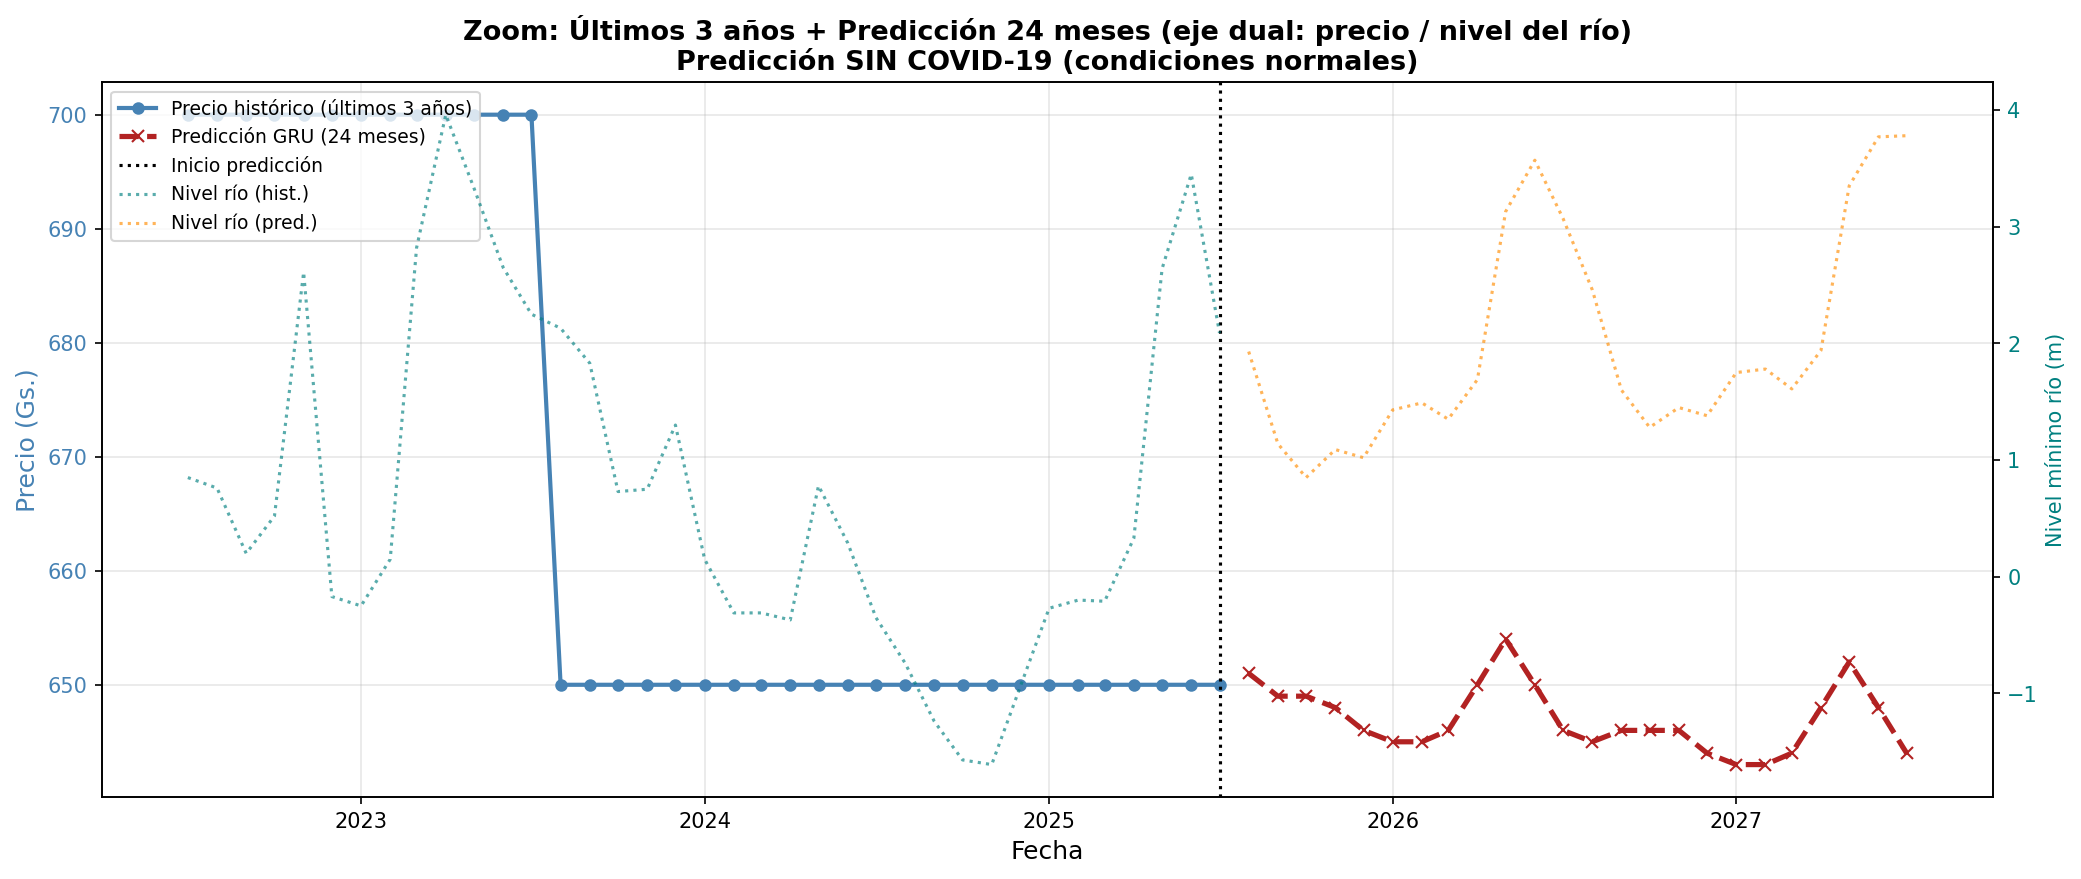
\includegraphics[width=\textwidth]{predicciones/prediccion_ladrillo_gru/resultados_sin_covid/final_07_prediccion_zoom_dual.png}
    \caption{Zoom sobre la transición entre datos observados y pronóstico GRU del ladrillo --- escenario sin pandemia.}
    \label{fig:gru_ladrillo_zoom_sin_covid}
\end{figure}

\begin{figure}[htbp]
    \centering
    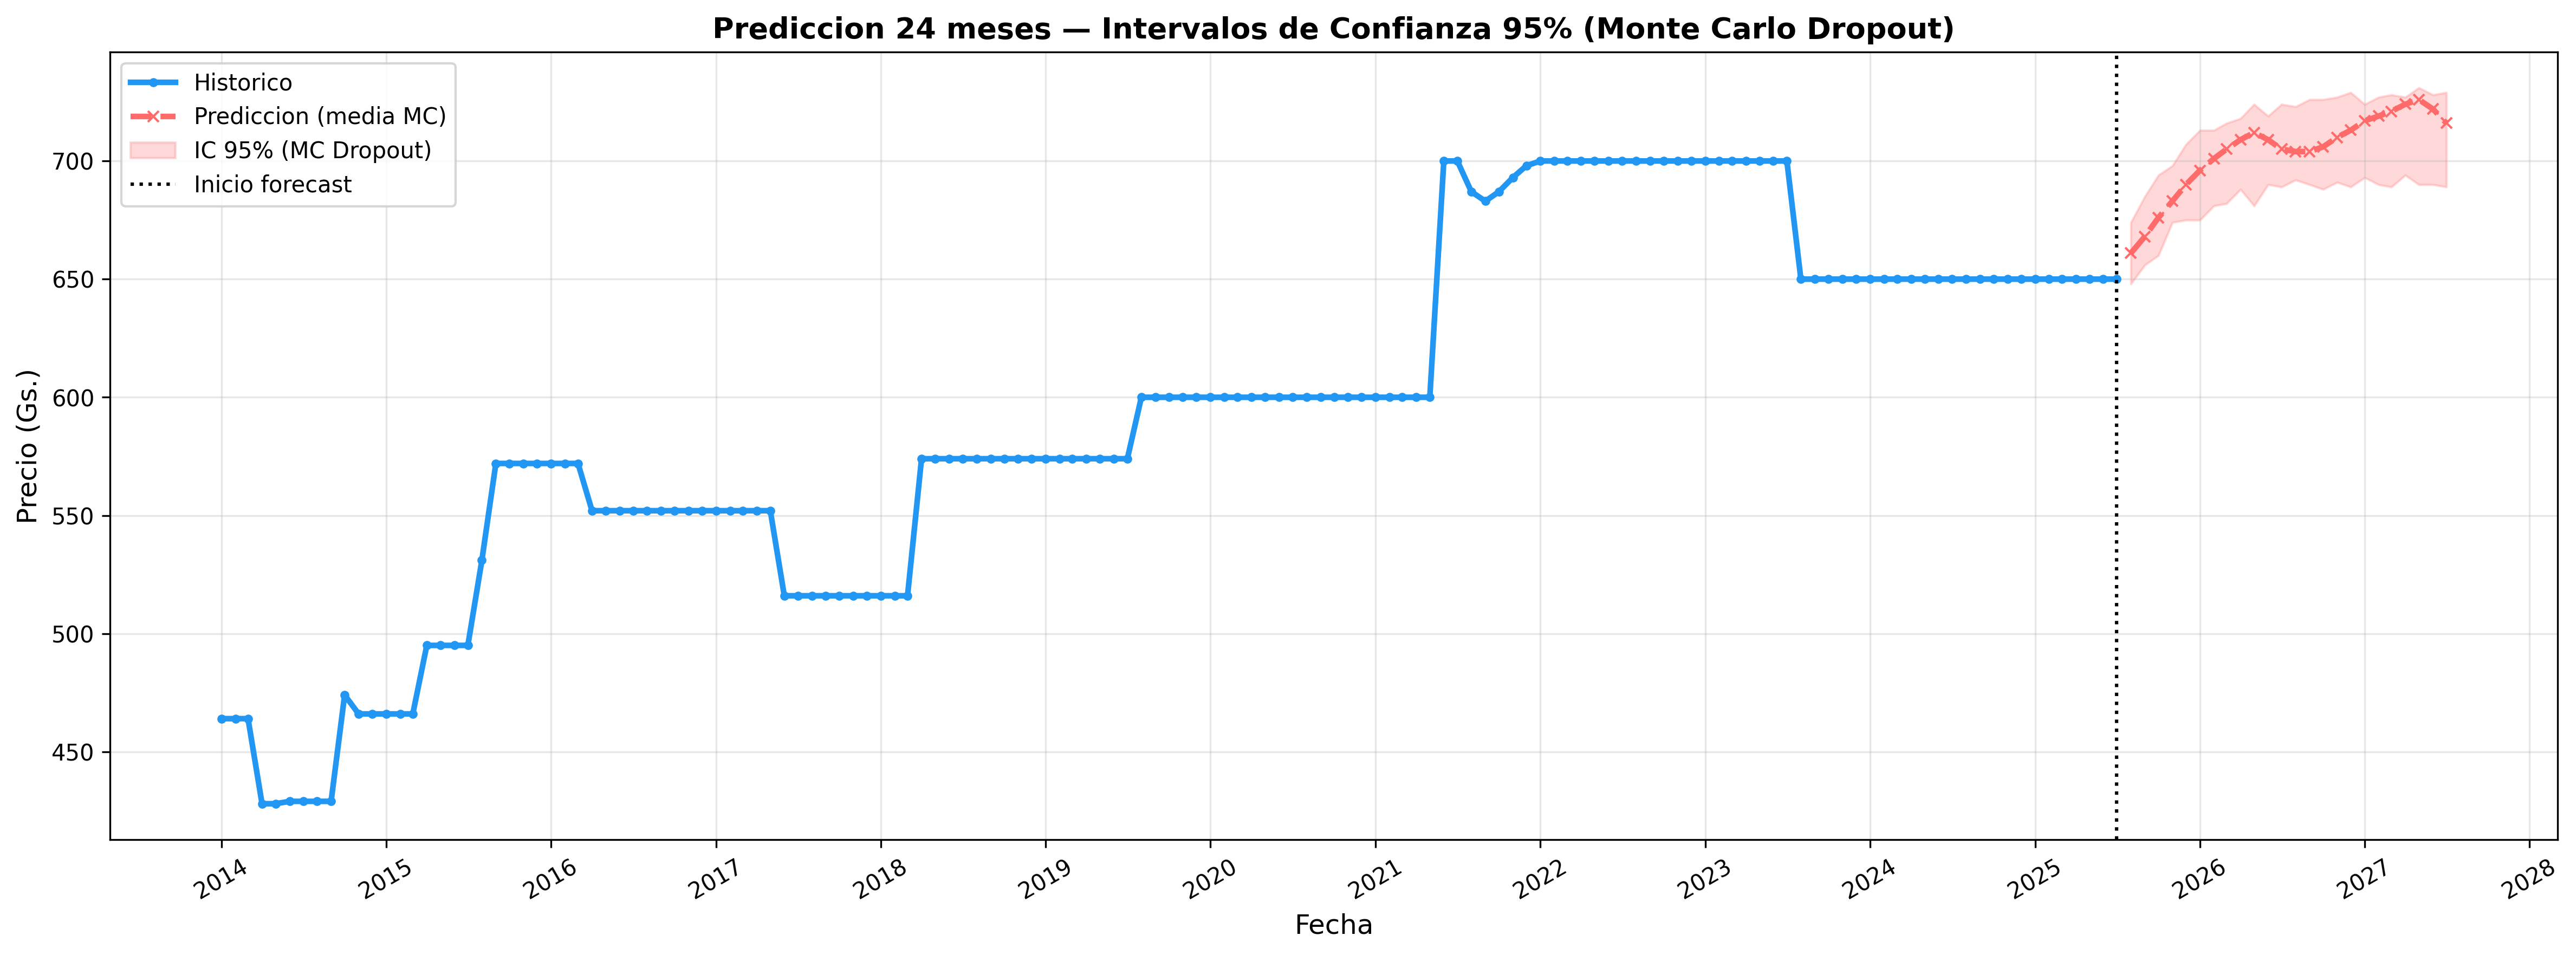
\includegraphics[width=\textwidth]{predicciones/prediccion_ladrillo_gru/resultados_sin_covid/forecast_ic_monte_carlo.png}
    \caption{IC Monte Carlo Dropout del pronóstico GRU para ladrillo --- escenario sin pandemia.}
    \label{fig:gru_ladrillo_ic_sin_covid}
\end{figure}

\justify
El modelo GRU proyecta, bajo el escenario sin pandemia, un precio del ladrillo en el rango de Gs.~662 a Gs.~726 a lo largo del horizonte de 24 meses. La amplitud del intervalo refleja la incertidumbre acumulada en las predicciones recursivas, aunque su magnitud sigue siendo moderada para una proyección de dos años.

% ------ LADRILLO GRU CON COVID ------
\clearpage
\subsubsection{Escenario con Efecto Pandémico}

\paragraph{Hiperparámetros y Arquitectura}

\justify
Para el escenario con pandemia, la búsqueda con Optuna (261 ensayos, 171,2 min) convergió a la misma configuración que el escenario sin pandemia: una GRU unidireccional con 64 unidades ocultas, Adam con $\eta = 0{,}008441$ y \textit{weight decay} $1{,}04 \times 10^{-6}$, \textit{lookback} de 3 meses, \textit{batch size} de 8, \textit{dropout} de 0{,}05, \textit{dropout} recurrente de 0{,}2 y \textit{scheduler} StepLR. Los 13.889 parámetros entrenables son idénticos al escenario sin pandemia. La Tabla~\ref{tab:gru_ladrillo_cc_arq} resume estos parámetros.

\begin{table}[htbp]
    \centering
    \caption{Hiperparámetros del modelo GRU para ladrillo --- escenario con pandemia.}
    \label{tab:gru_ladrillo_cc_arq}
    \begin{tabular}{ll}
        \toprule
        \textbf{Hiperparámetro} & \textbf{Valor} \\
        \midrule
        Capas GRU              & 1 (unidireccional) \\
        Unidades ocultas       & 64 \\
        Lookback               & 3 meses \\
        Optimizador            & Adam ($\eta=0{,}008441$, WD $=1{,}04 \times 10^{-6}$) \\
        Batch size             & 8 \\
        Dropout / Rec.\ dropout & 0{,}05 / 0{,}2 \\
        Scheduler              & StepLR \\
        Parámetros entrenables & 13.889 \\
        \bottomrule
    \end{tabular}
\end{table}

\paragraph{Curva de Aprendizaje}

\begin{figure}[htbp]
    \centering
    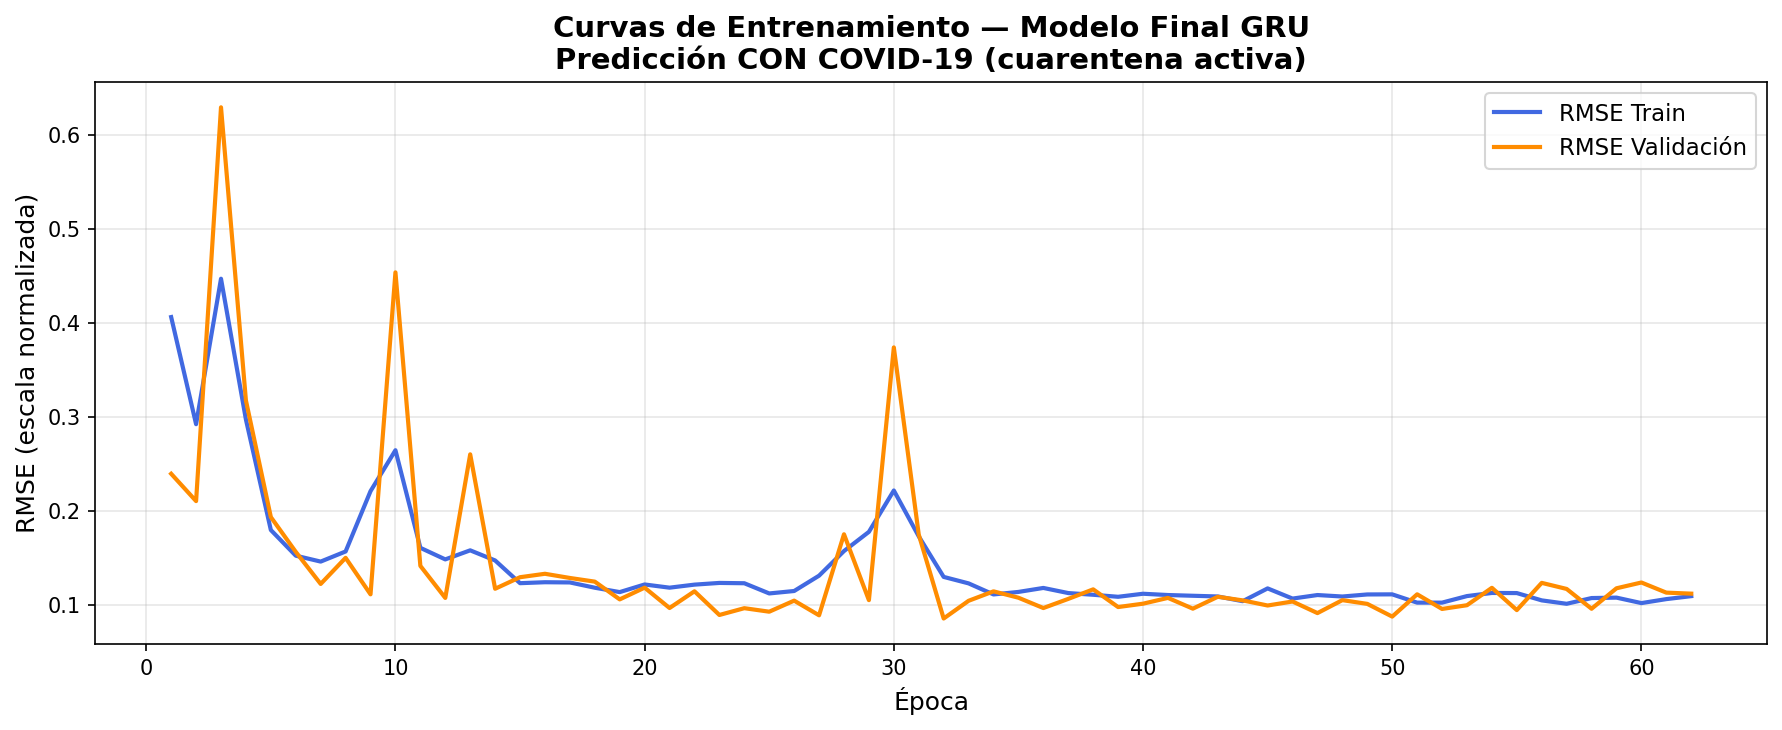
\includegraphics[width=\textwidth]{predicciones/prediccion_ladrillo_gru/resultados_con_covid/final_01_curvas_entrenamiento.png}
    \caption{Curvas de aprendizaje del modelo GRU para ladrillo --- escenario con pandemia.}
    \label{fig:gru_ladrillo_curva_cc}
\end{figure}

\paragraph{Métricas de Evaluación}

\begin{table}[htbp]
    \centering
    \caption{Desempeño del modelo GRU para ladrillo --- escenario con pandemia: RMSE en train, val y test.}
    \label{tab:gru_ladrillo_cc_metricas}
    \begin{tabular}{lrrr}
        \toprule
        \textbf{Métrica} & \textbf{Train} & \textbf{Val} & \textbf{Test} \\
        \midrule
        RMSE (Gs.) & 15{,}56 & 11{,}53 & 11{,}88 \\
        \bottomrule
    \end{tabular}
\end{table}

\justify
El RMSE de prueba del escenario con pandemia (Gs.~11{,}88) es idéntico al del escenario sin pandemia, resultado esperable dado que la búsqueda de hiperparámetros convergió a la misma configuración. El RMSE de validación de Gs.~11{,}53 también coincide, confirmando que ambos modelos son funcionalmente equivalentes salvo por el valor de la variable indicadora de pandemia durante la predicción futura.

\paragraph{Evaluación sobre el Conjunto de Prueba}

\begin{figure}[htbp]
    \centering
    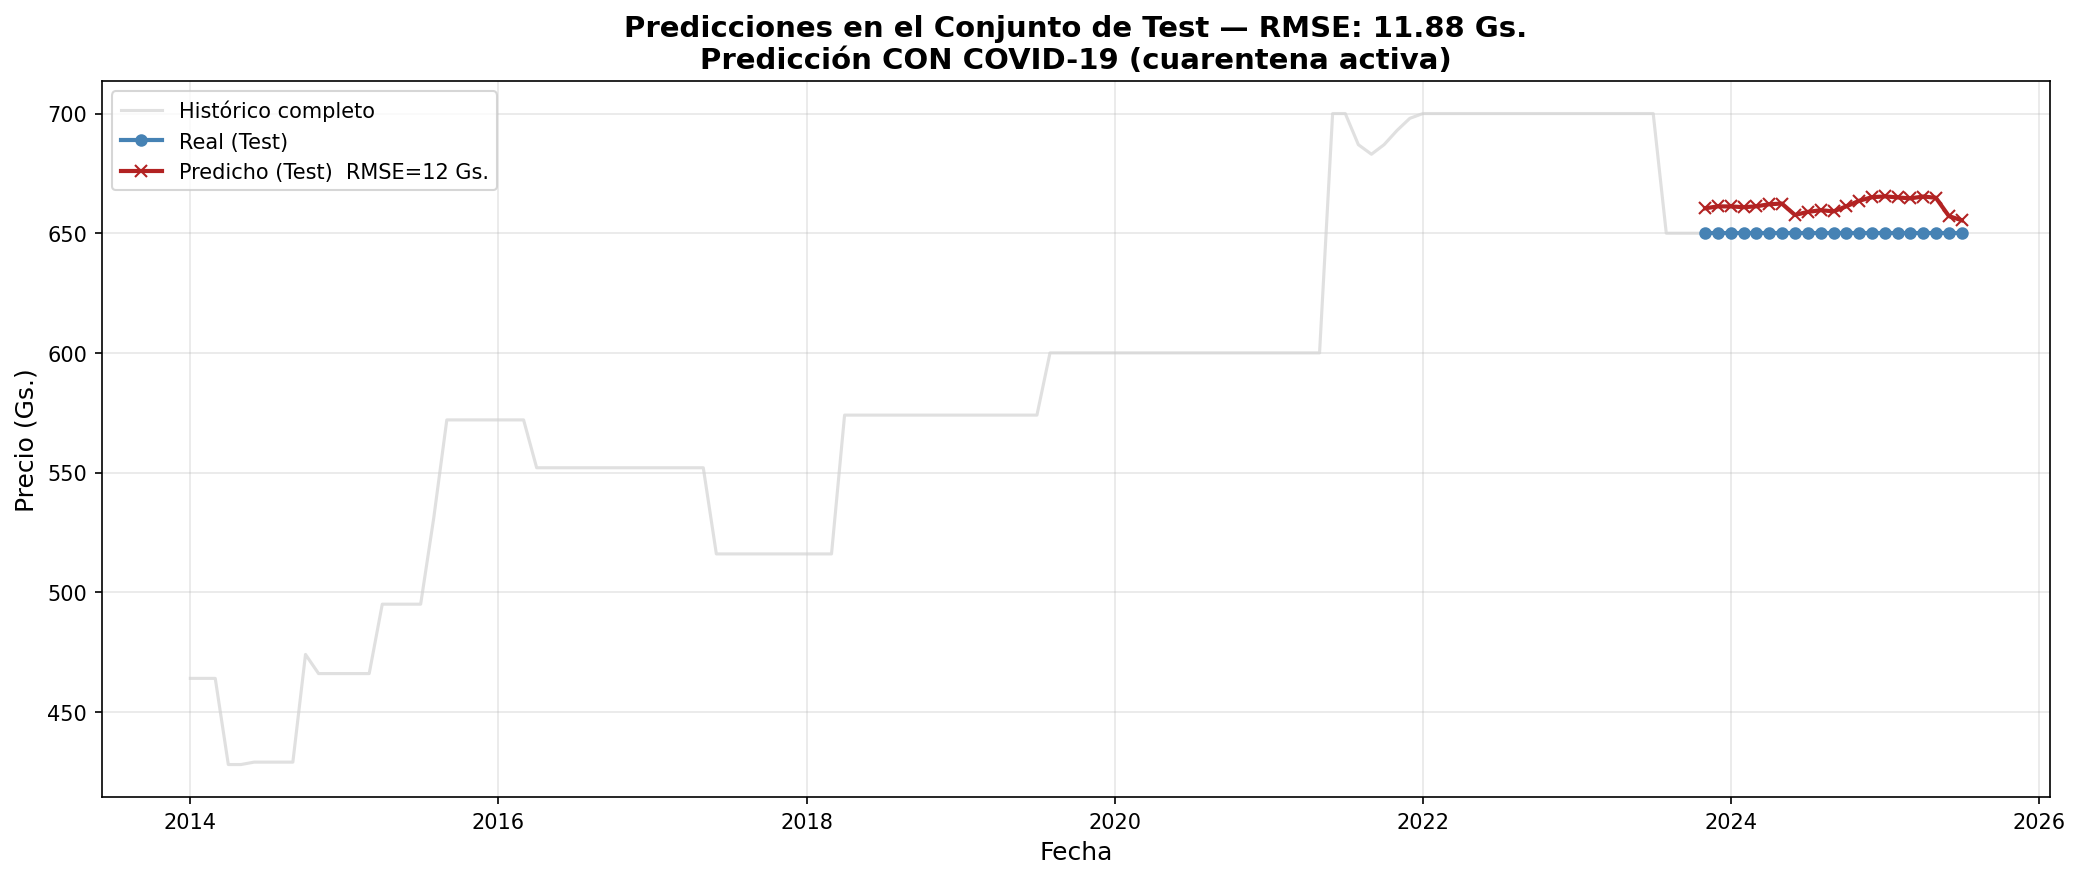
\includegraphics[width=\textwidth]{predicciones/prediccion_ladrillo_gru/resultados_con_covid/final_02_prediccion_test_serie.png}
    \caption{Predicción GRU vs.\ valores reales del precio del ladrillo --- escenario con pandemia, conjunto de prueba.}
    \label{fig:gru_ladrillo_test_cc}
\end{figure}

\begin{figure}[htbp]
    \centering
    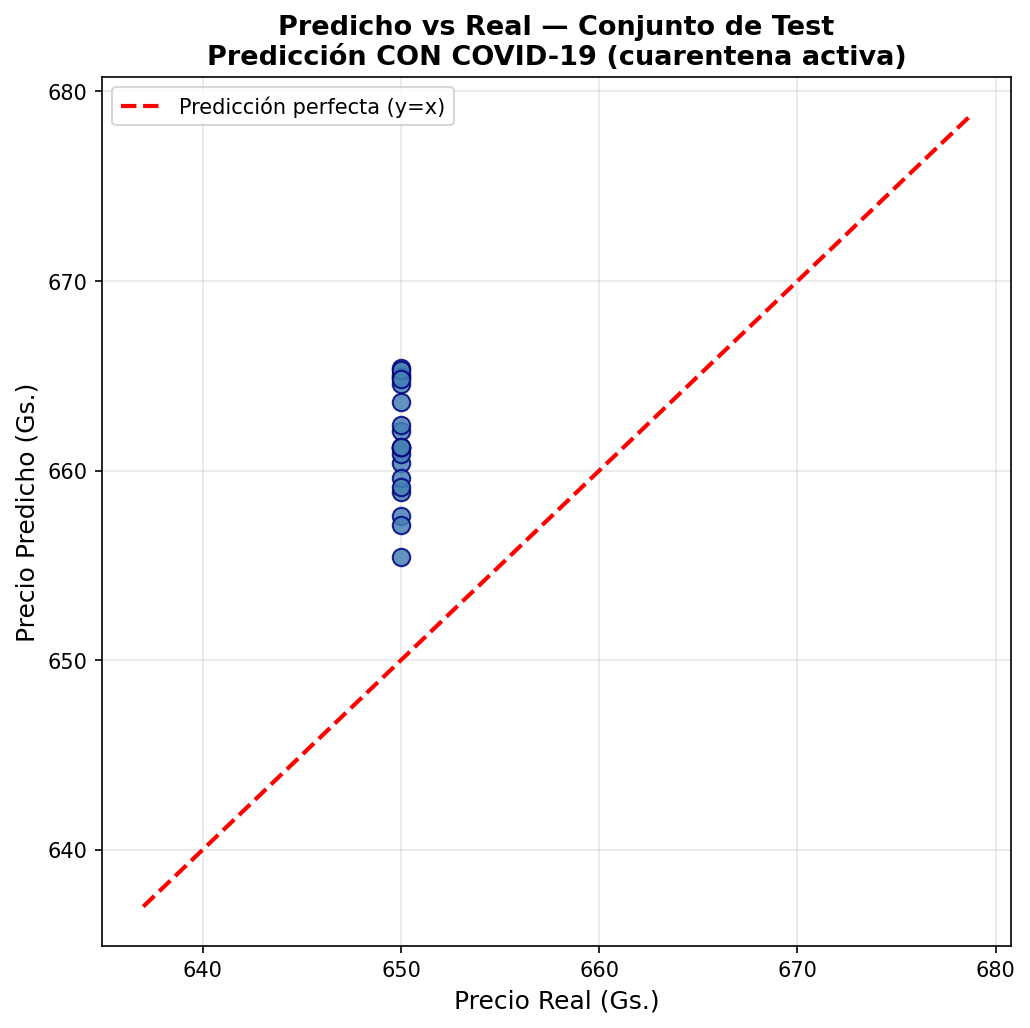
\includegraphics[width=0.8\textwidth]{predicciones/prediccion_ladrillo_gru/resultados_con_covid/final_03_scatter_test.png}
    \caption{Diagrama de dispersión: precio predicho vs.\ real del ladrillo --- escenario con pandemia (GRU).}
    \label{fig:gru_ladrillo_scatter_cc}
\end{figure}

\begin{figure}[htbp]
    \centering
    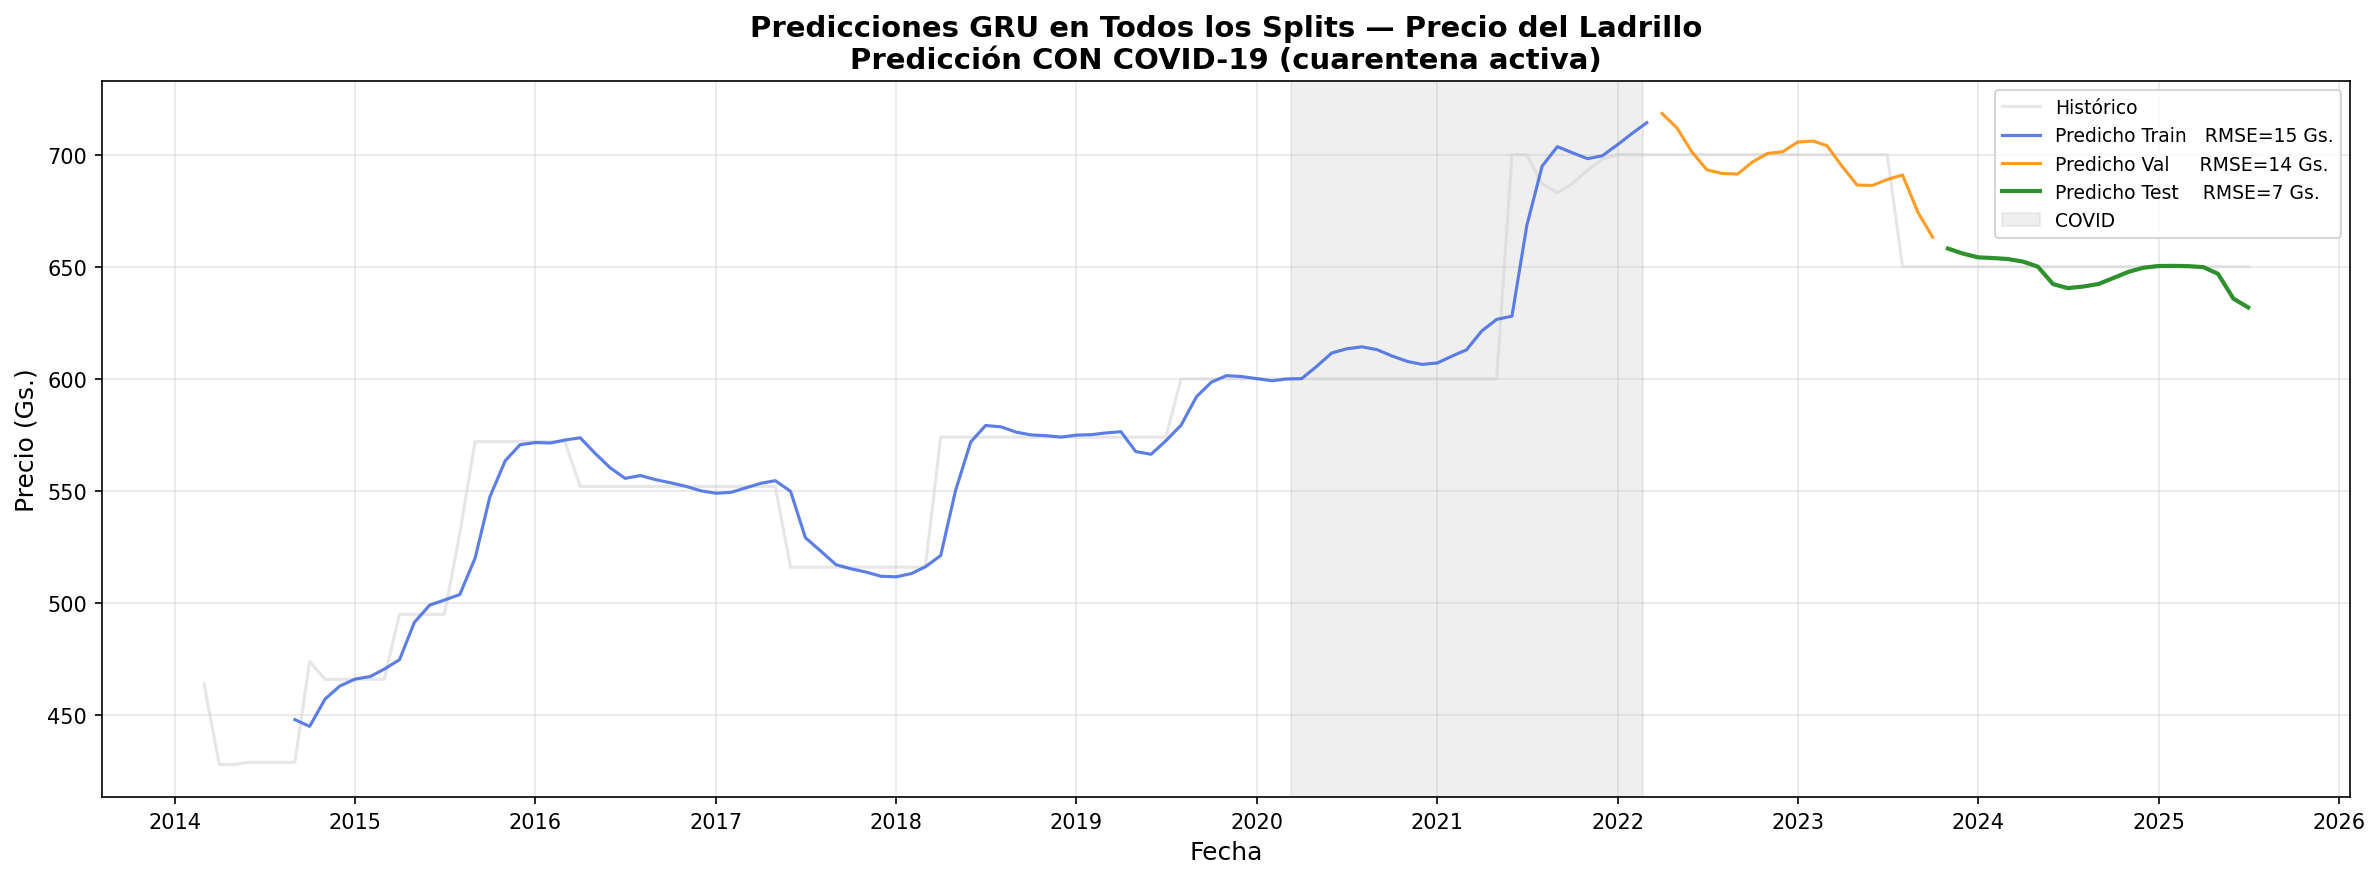
\includegraphics[width=\textwidth]{predicciones/prediccion_ladrillo_gru/resultados_con_covid/final_05_todos_splits.png}
    \caption{Ajuste del modelo GRU del ladrillo sobre las tres particiones --- escenario con pandemia.}
    \label{fig:gru_ladrillo_splits_cc}
\end{figure}

\clearpage
\paragraph{Análisis de Residuos}

\begin{figure}[htbp]
    \centering
    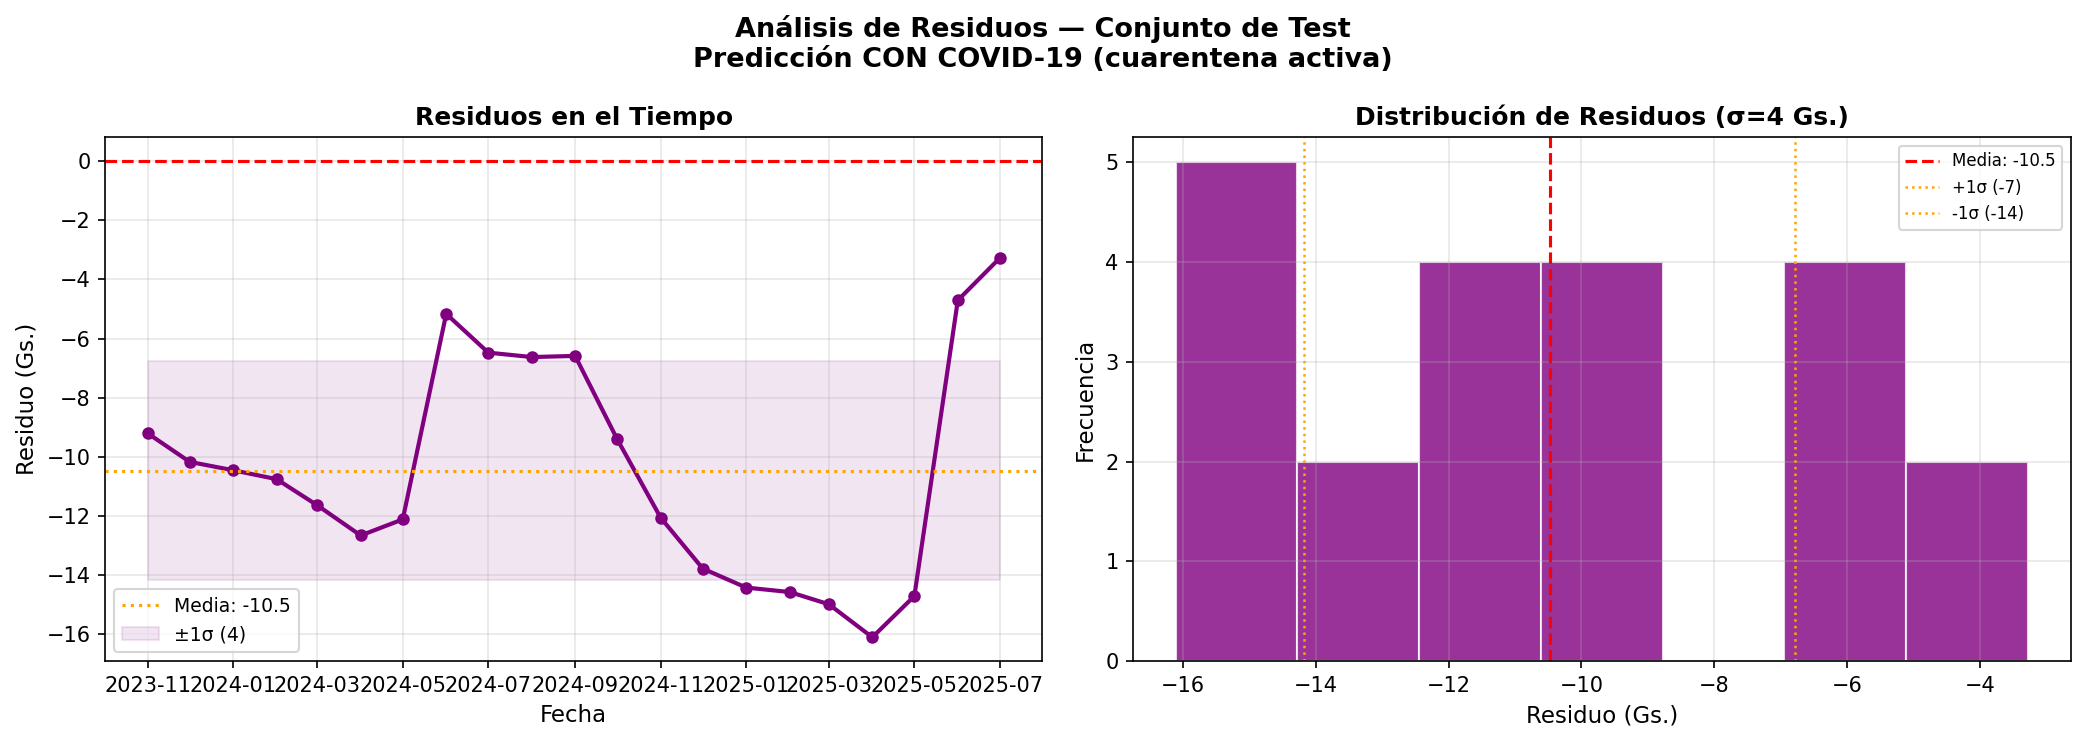
\includegraphics[width=\textwidth]{predicciones/prediccion_ladrillo_gru/resultados_con_covid/final_04_residuos.png}
    \caption{Residuos del modelo GRU para ladrillo --- escenario con pandemia, conjunto de prueba.}
    \label{fig:gru_ladrillo_res_cc}
\end{figure}

\begin{figure}[htbp]
    \centering
    \includegraphics[width=0.8\textwidth]{predicciones/prediccion_ladrillo_gru/resultados_con_covid/residuos_histograma.png}
    \caption{Histograma de residuos del modelo GRU para ladrillo --- escenario con pandemia.}
    \label{fig:gru_ladrillo_reshist_cc}
\end{figure}

\begin{figure}[htbp]
    \centering
    \includegraphics[width=\textwidth]{predicciones/prediccion_ladrillo_gru/resultados_con_covid/residuos_acf_pacf.png}
    \caption{ACF y PACF de los residuos del modelo GRU para ladrillo --- escenario con pandemia.}
    \label{fig:gru_ladrillo_acf_cc}
\end{figure}

\justify
El test de Ljung-Box sobre los residuos del conjunto de prueba muestra un $p$-valor de 0,009 a 10 rezagos (rechaza $H_0$) y de $1{,}13 \times 10^{-9}$ a 20 rezagos (rechaza fuertemente $H_0$). Este resultado indica la presencia de autocorrelación residual significativa en el modelo con pandemia, en contraste con el comportamiento de ruido blanco logrado por el modelo sin pandemia. La mayor autocorrelación residual sugiere que la configuración predeterminada del escenario con pandemia no captura tan eficientemente la estructura temporal de la serie del ladrillo como lo hace el modelo más compacto y propiamente optimizado.

\clearpage
\paragraph{Pronóstico a 24 Meses}

\begin{figure}[htbp]
    \centering
    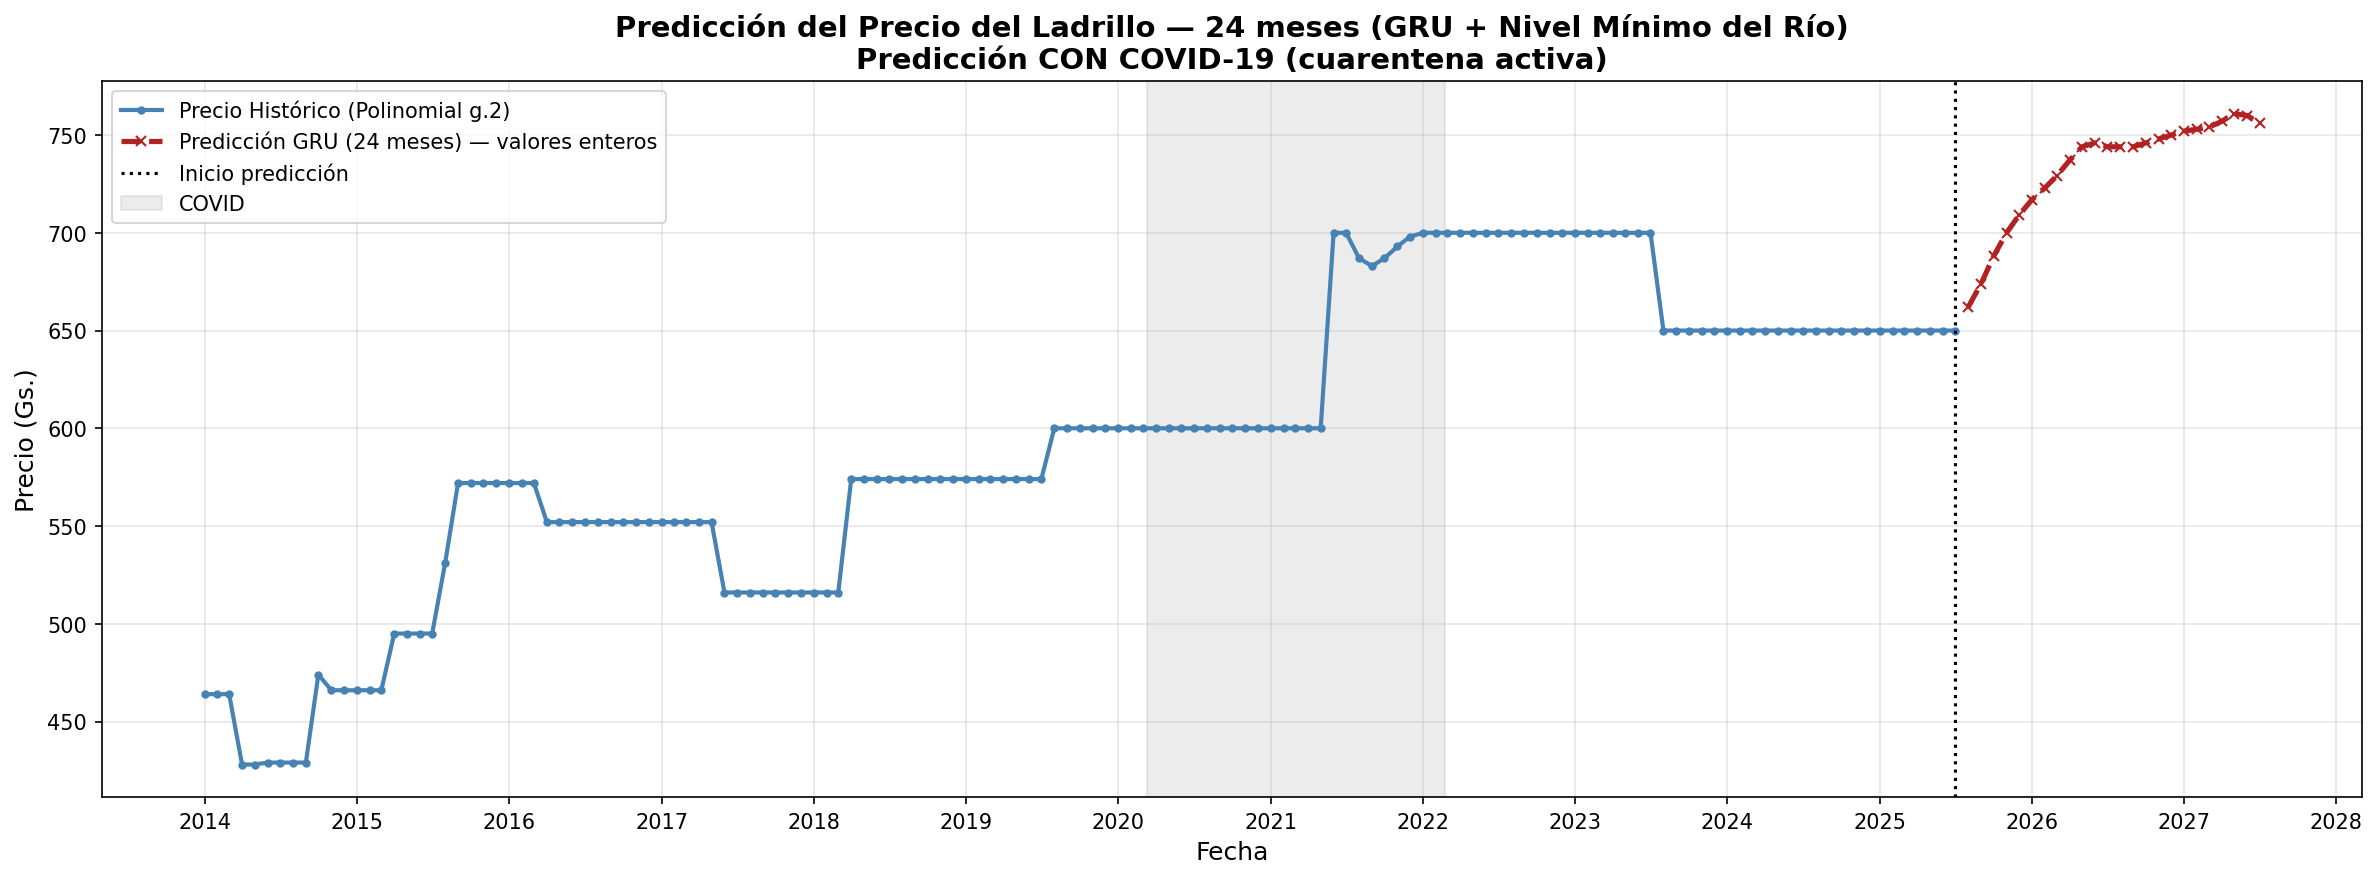
\includegraphics[width=\textwidth]{predicciones/prediccion_ladrillo_gru/resultados_con_covid/final_06_prediccion_futura_completa.png}
    \caption{Pronóstico GRU del precio del ladrillo a 24 meses --- escenario con pandemia: serie histórica y proyección.}
    \label{fig:gru_ladrillo_pred_con_covid}
\end{figure}

\begin{figure}[htbp]
    \centering
    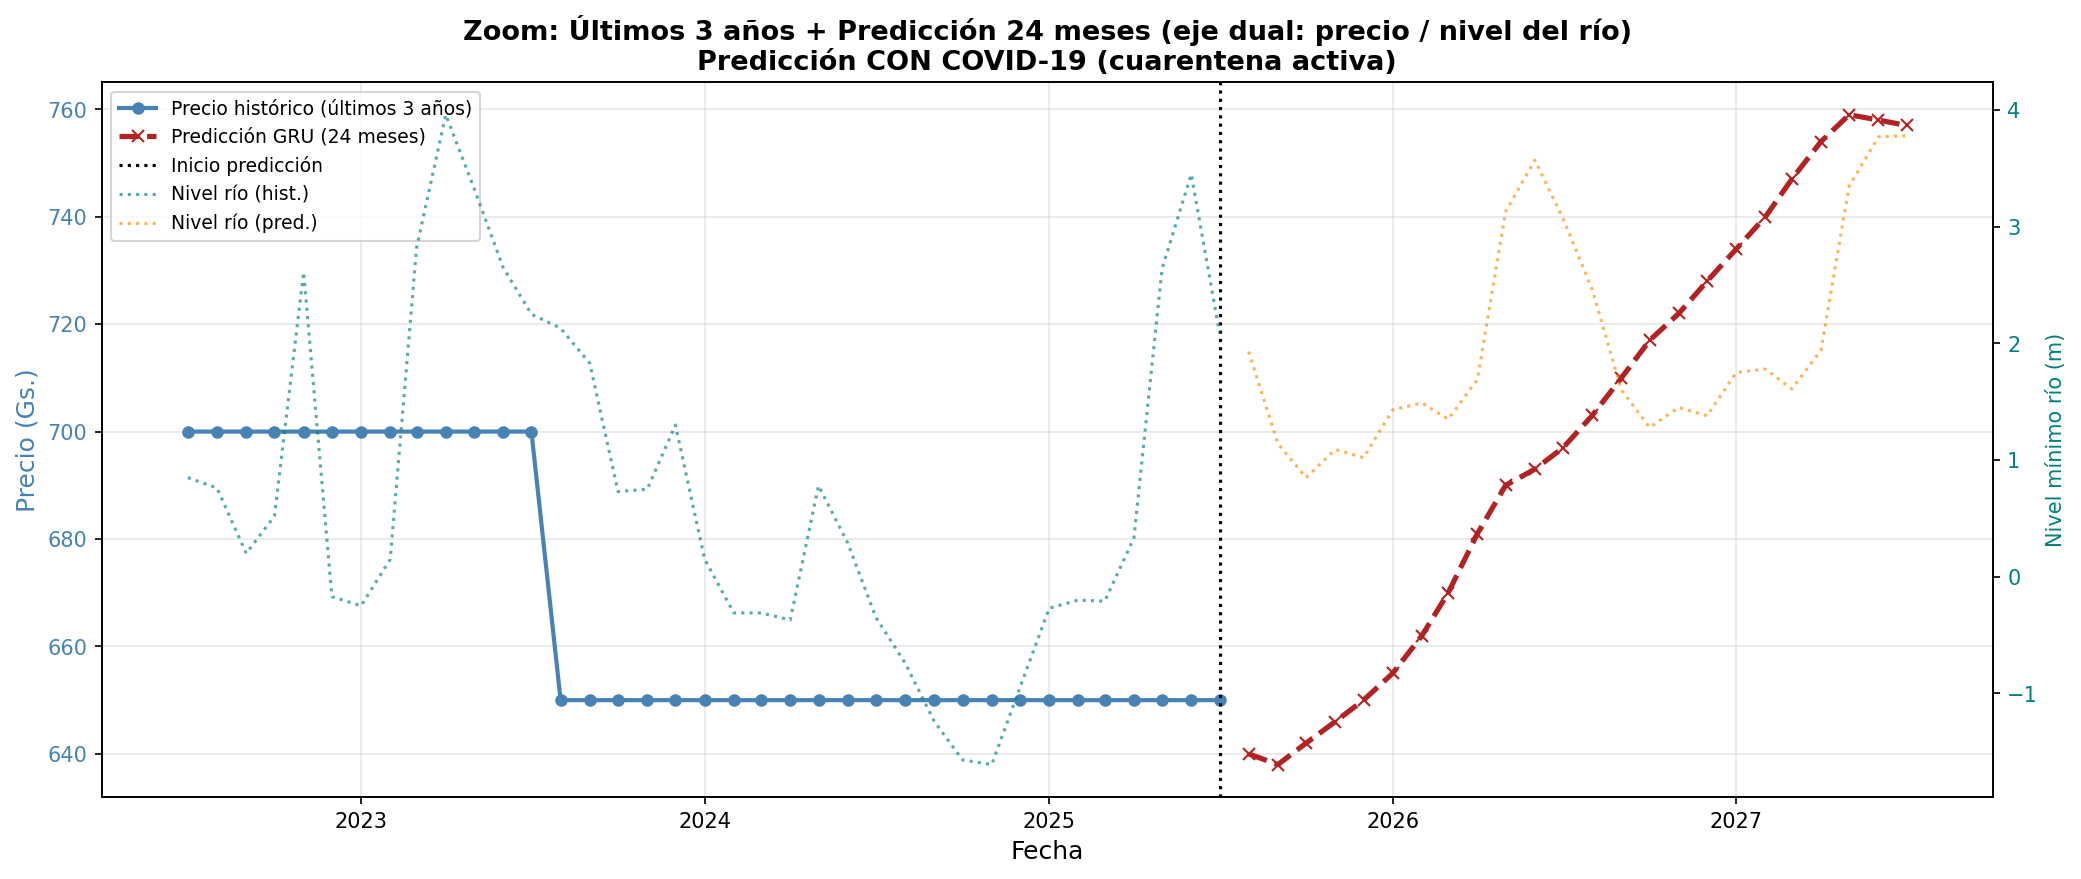
\includegraphics[width=\textwidth]{predicciones/prediccion_ladrillo_gru/resultados_con_covid/final_07_prediccion_zoom_dual.png}
    \caption{Zoom sobre la transición entre datos observados y pronóstico GRU del ladrillo --- escenario con pandemia.}
    \label{fig:gru_ladrillo_zoom_con_covid}
\end{figure}

\begin{figure}[htbp]
    \centering
    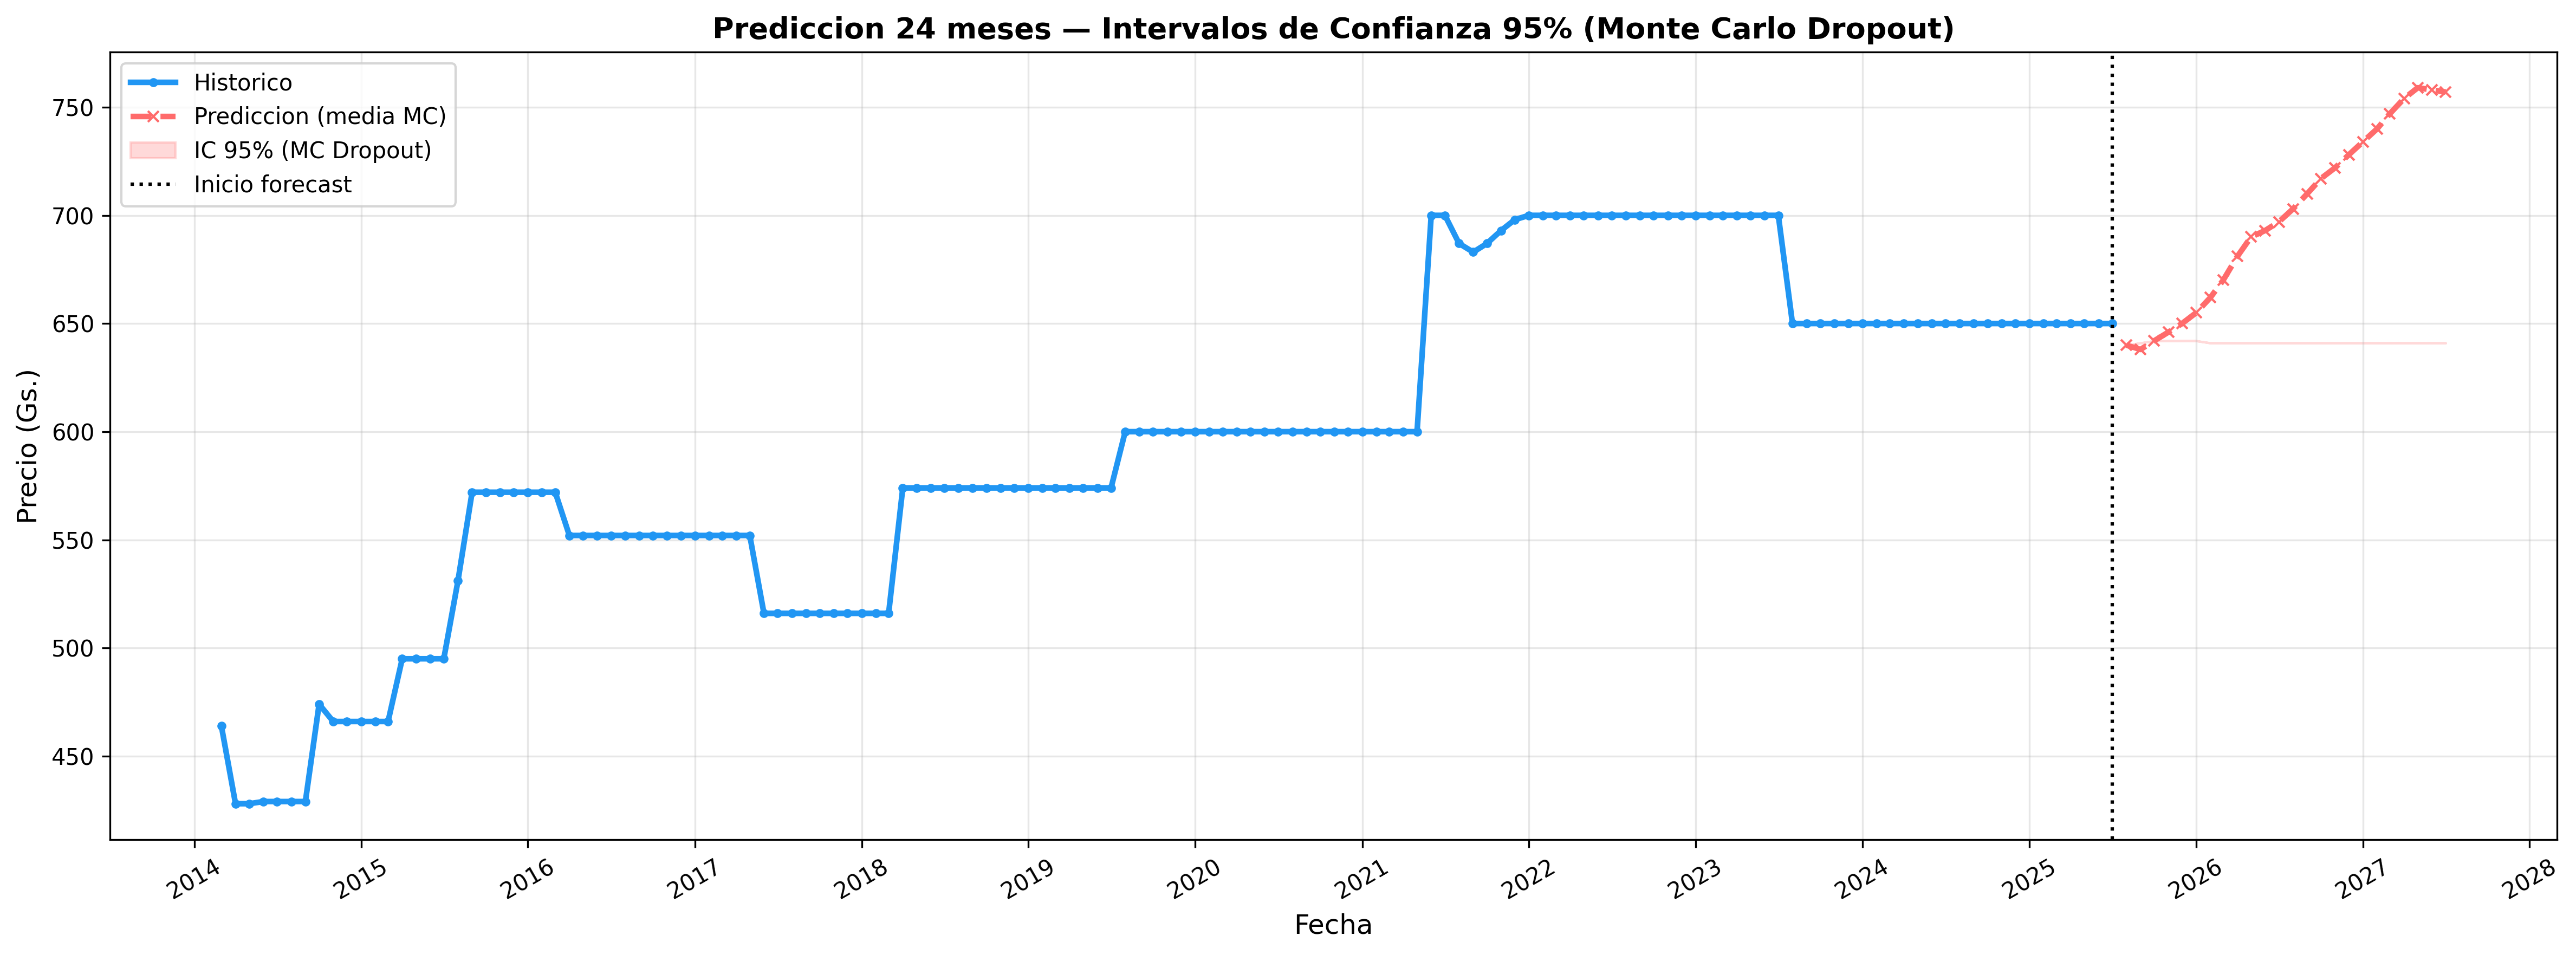
\includegraphics[width=\textwidth]{predicciones/prediccion_ladrillo_gru/resultados_con_covid/forecast_ic_monte_carlo.png}
    \caption{IC Monte Carlo Dropout del pronóstico GRU para ladrillo --- escenario con pandemia.}
    \label{fig:gru_ladrillo_ic_con_covid}
\end{figure}

\justify
Bajo el escenario con efecto pandémico, el rango de precios proyectado para el ladrillo se sitúa entre Gs.~662 y Gs.~761. El límite superior es ligeramente mayor que en el escenario sin pandemia (Gs.~726), lo que indica que el modelo captura un efecto alcista acumulado de la variable pandémica sobre el precio del ladrillo hacia el final del horizonte de predicción.

\justify
La divergencia en la interpretación del efecto pandémico entre los modelos GRU del cemento y del ladrillo es uno de los hallazgos más relevantes del estudio. Para el cemento, la GRU asoció la pandemia con una contracción de precios (rango Gs.~46.048--53.874 con pandemia versus Gs.~55.600--61.845 sin pandemia); para el ladrillo, el modelo capturó un efecto alcista moderado (Gs.~662--761 con pandemia versus Gs.~662--726 sin pandemia). Para el cemento, la pandemia fue interpretada como un factor de contracción de la demanda; para el ladrillo, como un leve impulso ascendente, lo que es más consistente con la evolución observada de los precios durante 2020--2022.



% 5. Discusión
\chapter{Discusión}
\thispagestyle{empty}
% ============================================================
% CAPÍTULO 6 — Discusión
% ============================================================

\section{Evaluaci\'{o}n del desempe\~{n}o del modelo Seasonal Autoregressive Integrated Moving Average with Exogenous Variables (SARIMAX)}
\vspace{0.3cm}

\justify
El resultado m\'{a}s llamativo de la modelaci\'{o}n SARIMAX es que la b\'{u}squeda exhaustiva por AIC seleccion\'{o}, tanto para el cemento como para el ladrillo, el orden $(0,1,0)(0,0,0)_{12}$. Este orden equivale a un paseo aleatorio (\textit{random walk}) con variables ex\'{o}genas: la mejor predicci\'{o}n del precio del mes siguiente es, simplemente, el precio del mes actual m\'{a}s la contribuci\'{o}n lineal de las covariables. La ausencia de t\'{e}rminos autorregresivos ($p=0$), de media m\'{o}vil ($q=0$) y de componentes estacionales ($P=D=Q=0$) indica que, una vez diferenciada, la serie de precios se comporta como ruido blanco y que el modelo no encuentra estructura temporal adicional que pueda explotar. Este hallazgo es consistente con la din\'{a}mica de los mercados de insumos de construcci\'{o}n en Paraguay, donde los ajustes de precios son infrecuentes y tienden a mantenerse estables durante per\'{i}odos prolongados antes de registrar saltos discretos.

\justify
El desempe\~{n}o del SARIMAX sobre el conjunto de prueba difiri\'{o} significativamente entre materiales (Tablas \ref{tab:sarimax_metricas_prueba} y \ref{tab:sarimax_ladrillo_metricas_prueba}). Para el ladrillo, el RMSE de prueba fue de apenas Gs.~4,54, resultado que se explica porque durante los 22 meses del per\'{i}odo de evaluaci\'{o}n el precio se mantuvo constante en Gs.~650; en ese contexto, el paseo aleatorio ---que predice el \'{u}ltimo valor observado--- genera errores m\'{i}nimos y el $R^{2}$ resulta indefinido o cercano a cero por la escasa varianza del per\'{i}odo. Para el cemento, en cambio, el precio cay\'{o} de Gs.~60.000 a Gs.~55.000 en enero de 2024 y el modelo no anticip\'{o} ese ajuste, lo que se tradujo en un RMSE de prueba de Gs.~4.842,33 ---equivalente al tama\~{n}o del salto que el paseo aleatorio no pudo capturar---.

\justify
La validaci\'{o}n cruzada por ventana deslizante (\textit{rolling forecast}) ofrece una perspectiva m\'{a}s representativa del desempe\~{n}o real al abarcar todo el per\'{i}odo hist\'{o}rico, incluyendo los a\~{n}os de alta volatilidad asociados a la pandemia y a las variaciones hidrol\'{o}gicas. Bajo esta evaluaci\'{o}n, el $R^{2}$ sube a 0{,}7586 para el cemento (Tabla~\ref{tab:sarimax_metricas_cv}) y a 0{,}8193 para el ladrillo (Tabla~\ref{tab:sarimax_ladrillo_metricas_cv}), con RMSE de validaci\'{o}n cruzada de 1.920{,}78~Gs. y 9{,}52~Gs. respectivamente. Estos valores confirman la utilidad pr\'{a}ctica del SARIMAX para la estimaci\'{o}n presupuestaria a corto plazo cuando las series no presentan grandes saltos inesperados. El mejor ajuste del ladrillo puede atribuirse a que este material presenta per\'{i}odos prolongados de estabilidad, patr\'{o}n que el paseo aleatorio captura con naturalidad.

\justify
Un hallazgo cr\'{i}tico es que las variables ex\'{o}genas ---el nivel del r\'{i}o Paraguay y la variable binaria de cuarentena--- resultaron estad\'{i}sticamente no significativas en ambos modelos. Para el cemento, el coeficiente del nivel del r\'{i}o fue de $-55{,}34$~Gs./m con un $p$-valor de 0{,}895 (Tabla~\ref{tab:sarimax_params}); para el ladrillo, fue de $-1{,}93$~Gs./m con $p=0{,}302$ (Tabla~\ref{tab:sarimax_ladrillo_params}). La variable de cuarentena present\'{o} $p$-valores de 1{,}000 y 0{,}999, respectivamente. Esta no significancia no implica que dichas variables carezcan de influencia real sobre los precios, sino que el modelo lineal integrado ---al absorber la tendencia mediante la diferenciaci\'{o}n--- pierde la capacidad de detectar efectos que se manifiestan de forma no lineal, asim\'{e}trica o con retardos variables. El SARIMAX asume una relaci\'{o}n lineal y contempor\'{a}nea entre las covariables y la variable dependiente, supuesto que resulta insuficiente para capturar la complejidad de fen\'{o}menos como la pandemia de COVID-19, cuyo impacto sobre los precios se propag\'{o} a trav\'{e}s de m\'{u}ltiples canales (interrupciones log\'{i}sticas, ca\'{i}da de demanda, especulaci\'{o}n, reactivaci\'{o}n diferida) y con desfases temporales heterog\'{e}neos.

\justify
La insensibilidad del SARIMAX ante el escenario pand\'{e}mico lo confirma cuantitativamente: la diferencia entre el pron\'{o}stico con y sin la variable de cuarentena activa fue de apenas $-23{,}48$~Gs./mes para el cemento (Figuras~\ref{fig:sarimax_cemento_sin_covid} y \ref{fig:sarimax_cemento_con_covid}) y de $-0{,}82$~Gs./mes para el ladrillo (Figuras~\ref{fig:sarimax_ladrillo_sin_covid} y \ref{fig:sarimax_ladrillo_con_covid}), valores pr\'{a}cticamente despreciables frente a los niveles de precios de las series (Gs.~55.000 y Gs.~650, respectivamente). Esta limitaci\'{o}n constituye una de las motivaciones principales para explorar los modelos de aprendizaje profundo, que s\'{i} disponen de la flexibilidad no lineal necesaria para diferenciar escenarios.

\justify
En cuanto a los diagn\'{o}sticos estad\'{i}sticos, los residuos de ambos modelos SARIMAX superaron el test de Ljung-Box ($p>0{,}05$ en rezagos 10 y 20), lo que confirma la ausencia de autocorrelaci\'{o}n serial y valida que el modelo ha capturado adecuadamente la estructura din\'{a}mica lineal de las series. Sin embargo, el test de Shapiro-Wilk rechaz\'{o} la normalidad en ambos casos (Figuras~\ref{fig:sarimax_residuos} y \ref{fig:sarimax_ladrillo_residuos}), con valores de curtosis de 49{,}47 y 26{,}69 para cemento y ladrillo, respectivamente. Esta no normalidad ---atribuible a observaciones extremas durante el per\'{i}odo pand\'{e}mico--- no invalida las estimaciones puntuales, pero s\'{i} compromete la fiabilidad de los intervalos de confianza calculados bajo el supuesto gaussiano, que se ensanchan r\'{a}pidamente a medida que crece el horizonte de predicci\'{o}n. Para el cemento, el intervalo al 95\,\% pas\'{o} de Gs.~[49.535 -- 60.483] en el primer mes a Gs.~[28.089 -- 81.724] en el mes 24 (Tabla~\ref{tab:sarimax_pronostico}), un rango que cubre pr\'{a}cticamente todo el espectro hist\'{o}rico de la serie y limita la utilidad pr\'{a}ctica del pron\'{o}stico a largo plazo.

% ============================================================
\section{Evaluaci\'{o}n del desempe\~{n}o del modelo Long Short-Term Memory (LSTM)}
\vspace{0.3cm}

\justify
La primera aplicaci\'{o}n del modelo LSTM en este trabajo fue la predicci\'{o}n del nivel diario del r\'{i}o Paraguay, variable ex\'{o}gena central de los modelos de precios. Los resultados fueron notables: un RMSE de prueba de 0{,}0449~m ---menos de 5{,}3~cm de error sobre una serie que oscila entre $-2$ y $+8$~metros--- y un coeficiente de Nash-Sutcliffe (NSE) de 0{,}9992 (Tabla~\ref{tab:metricas_lstm_rio}). Este nivel de precisi\'{o}n, obtenido con una arquitectura de una sola capa LSTM de 512 unidades ocultas y una ventana de entrada de 180 d\'{i}as (Tabla~\ref{tab:hiperparametros_lstm_rio}), valida la capacidad de las redes LSTM para modelar series hidrol\'{o}gicas con din\'{a}micas estacionales complejas. La estrategia recursiva de predicci\'{o}n, en la que cada proyecci\'{o}n diaria se reincorpora como entrada para el paso siguiente, logr\'{o} generar un pron\'{o}stico a 730 d\'{i}as que reproduce correctamente los ciclos de crecida y estiaje del r\'{i}o (Figuras~\ref{fig:historico_prediccion} y \ref{fig:climatologia_prediccion}), aunque con una amplitud de oscilaci\'{o}n ligeramente atenuada respecto a la climatolog\'{i}a hist\'{o}rica ---comportamiento esperable en horizontes de proyecci\'{o}n extendidos donde la estrategia recursiva tiende a regresar las predicciones hacia la media---.

\justify
Esta predicci\'{o}n del nivel del r\'{i}o se utiliz\'{o} como variable ex\'{o}gena en todos los modelos de precios subsiguientes. Es importante se\~{n}alar que cualquier error en la proyecci\'{o}n hidrol\'{o}gica se propaga a las predicciones de precios, de modo que la cadena de modelaci\'{o}n introduce una fuente adicional de incertidumbre que no queda reflejada en los intervalos de confianza de los modelos de precios. No obstante, dado que el RMSE del modelo del r\'{i}o representa menos del 0{,}6\,\% del rango total de la variable, esta propagaci\'{o}n de errores puede considerarse marginal.

\justify
Para la predicci\'{o}n del precio del cemento, Optuna seleccion\'{o} una arquitectura compacta: una capa LSTM unidireccional con 64 unidades ocultas, sin \textit{dropout} ni planificador de tasa de aprendizaje, y con una ventana de entrada de 6 meses (Tabla~\ref{tab:lstm_cemento_hiper}). En el escenario sin pandemia, el modelo totaliz\'{o} 18.241 par\'{a}metros entrenables y alcanz\'{o} un RMSE de prueba de 5.432{,}05~Gs.\ (Tabla~\ref{tab:lstm_cemento_metricas}). En el escenario con pandemia, Optuna seleccion\'{o} una arquitectura bidireccional con \textit{dropout} y planificador ReduceLROnPlateau, resultando en 36.481 par\'{a}metros y un RMSE de prueba de 4.394{,}96~Gs. ---el mejor resultado individual para el cemento en este estudio---. Sin embargo, el an\'{a}lisis de residuos revel\'{o} autocorrelaci\'{o}n estad\'{i}sticamente significativa en los rezagos 10 ($p=0{,}017$) y 20 ($p=0{,}042$) del test de Ljung-Box (Figura~\ref{fig:lstm_cemento_acf_residuos}). Aunque los $p$-valores son cercanos al l\'{i}mite de significancia, este resultado indica que el modelo deja estructura temporal sin capturar en sus residuos, lo que podr\'{i}a traducirse en subestimaci\'{o}n de la incertidumbre cuando se emplean los intervalos de Monte Carlo Dropout. En el escenario sin pandemia, la ausencia de \textit{dropout} y de \textit{scheduler}, seleccionada por Optuna como configuraci\'{o}n \'{o}ptima, sugiere que la regularizaci\'{o}n L2 ($\lambda=10^{-5}$) fue suficiente para controlar el sobreajuste, pero no para eliminar toda la dependencia temporal en los errores.

\justify
El modelo LSTM del ladrillo constituye el mejor resultado individual de esta arquitectura. A diferencia del cemento, Optuna seleccion\'{o} una LSTM \textbf{bidireccional} con \textit{dropout} de 0{,}2, \textit{dropout} recurrente de 0{,}05 y planificador StepLR (Tabla~\ref{tab:lstm_ladrillo_hiper}), lo que result\'{o} en 36.481 par\'{a}metros entrenables ---aproximadamente el doble que el modelo del cemento sin pandemia---. El RMSE de prueba de 6{,}22~Gs.\ (escenario con pandemia) y 6{,}62~Gs.\ (sin pandemia) (Tabla~\ref{tab:lstm_ladrillo_metricas}) es notablemente bajo: representa un error relativo inferior al 2\,\% del rango hist\'{o}rico de la serie. El an\'{a}lisis de residuos mostr\'{o} un comportamiento m\'{a}s favorable que el del cemento: el test de Ljung-Box a 10 rezagos no rechaz\'{o} la hip\'{o}tesis nula ($p=0{,}237$), aunque s\'{i} lo hizo a 20 rezagos ($p<0{,}001$), indicando la presencia de patrones de dependencia en rezagos distantes que podr\'{i}an estar asociados a la estacionalidad no capturada completamente por las variables de entrada.

\justify
La selecci\'{o}n de una arquitectura bidireccional para el ladrillo es un hallazgo relevante. La bidireccionalidad permite al modelo procesar la secuencia temporal en ambas direcciones dentro de la ventana de entrada, lo que duplica la cantidad de informaci\'{o}n contextual disponible en cada paso. El hecho de que Optuna haya preferido esta configuraci\'{o}n para el ladrillo ---pero no para el cemento--- sugiere que la serie de precios del ladrillo, con sus ajustes escalonados y per\'{i}odos prolongados de estabilidad, se beneficia de la capacidad de la red bidireccional para ``mirar hacia adelante'' dentro de la ventana de contexto y anticipar los momentos de cambio. En contraste, la tendencia m\'{a}s continua del cemento se modela adecuadamente con una arquitectura unidireccional m\'{a}s simple.

\justify
En cuanto a la diferenciaci\'{o}n de escenarios pand\'{e}micos, el modelo LSTM mostr\'{o} un comportamiento consistente para ambos materiales: bajo el escenario con cuarentena activa, el l\'{i}mite superior del rango de predicci\'{o}n del cemento subi\'{o} de 62.197~Gs.\ a 73.374~Gs.\ ---un incremento del 18{,}1\,\%--- (Figuras~\ref{fig:lstm_cemento_pred_sin_covid} y \ref{fig:lstm_cemento_pred_con_covid}), mientras que para el ladrillo pas\'{o} de 706~Gs.\ a 757~Gs.\ ---un incremento del 7{,}2\,\%--- (Figuras~\ref{fig:lstm_ladrillo_pred_sin_covid} y \ref{fig:lstm_ladrillo_pred_con_covid}). Ambas direcciones son consistentes con lo ocurrido durante la pandemia real de 2020--2022, cuando las disrupciones en la cadena de suministro provocaron aumentos sostenidos en los precios de materiales de construcci\'{o}n. La menor magnitud del efecto en el ladrillo puede atribuirse a que este material, de producci\'{o}n predominantemente local con cadenas log\'{i}sticas m\'{a}s cortas, es menos sensible a las interrupciones del comercio internacional que afectaron particularmente al cemento.

% ============================================================
\section{Evaluaci\'{o}n del desempe\~{n}o del modelo Gated Recurrent Unit (GRU)}
\vspace{0.3cm}

\justify
La arquitectura GRU, que emplea dos compuertas (actualizaci\'{o}n y reinicio) frente a las tres de la LSTM (entrada, olvido y salida), fue evaluada como alternativa con menor complejidad param\'{e}trica. Para el cemento, Optuna seleccion\'{o} una configuraci\'{o}n con una capa GRU unidireccional de 64 unidades ocultas, \textit{dropout} de 0{,}1, optimizador Adam con $\eta=0{,}00732$ y planificador ReduceLROnPlateau (Tabla~\ref{tab:gru_cemento_arq}), resultando en 13.889 par\'{a}metros entrenables. El RMSE de prueba fue de 4.964{,}27~Gs.\ (Tabla~\ref{tab:gru_cemento_metricas}), superior al obtenido por la LSTM en el escenario con pandemia (4.394{,}96~Gs.). La selecci\'{o}n de \textit{dropout} por parte de Optuna ---ausente en el modelo LSTM del mismo material--- sugiere que la GRU, pese a su menor n\'{u}mero de par\'{a}metros, present\'{o} indicios de sobreajuste durante la b\'{u}squeda, posiblemente porque la simplificaci\'{o}n de compuertas reduce la capacidad de la red para gestionar la memoria de largo plazo en la serie del cemento, que exhibe una tendencia continua.

\justify
En cuanto al efecto pand\'{e}mico, la GRU del cemento mostr\'{o} una respuesta consistente con la LSTM: bajo el escenario con cuarentena, el l\'{i}mite superior del rango de predicci\'{o}n subi\'{o} de Gs.~63.852 a Gs.~65.337 ---un incremento del 2{,}3\,\%--- (Figuras~\ref{fig:gru_cemento_pred_sin_covid} y \ref{fig:gru_cemento_pred_con_covid}). Aunque la magnitud del efecto estimado por la GRU es considerablemente menor que el 18{,}1\,\% proyectado por la LSTM, ambos modelos coinciden en la direcci\'{o}n del impacto pand\'{e}mico sobre el cemento: una presi\'{o}n alcista coherente con las disrupciones en la cadena de suministros que elevaron los costos log\'{i}sticos durante 2020--2022.

\justify
El modelo GRU para el ladrillo, con 13.889 par\'{a}metros entrenables (Tabla~\ref{tab:gru_ladrillo_arq}), alcanz\'{o} un RMSE de prueba de 11{,}88~Gs.\ (Tabla~\ref{tab:gru_ladrillo_metricas}), resultado inferior tanto a la LSTM bidireccional del mismo material (6{,}22~Gs., 36.481 par\'{a}metros) como al modelo SARIMAX (4{,}54~Gs.). Este desempe\~{n}o indica que, para la serie del ladrillo ---caracterizada por ajustes escalonados y per\'{i}odos prolongados de estabilidad---, la arquitectura GRU unidireccional no logr\'{o} capturar los patrones de cambio con la misma efectividad que las alternativas evaluadas.

\justify
El an\'{a}lisis de residuos del GRU del ladrillo fue tambi\'{e}n el m\'{a}s favorable de todos los modelos de aprendizaje profundo evaluados: el test de Ljung-Box no rechaz\'{o} la hip\'{o}tesis nula de ausencia de autocorrelaci\'{o}n serial ni a 10 rezagos ($p=0{,}442$) ni a 20 rezagos ($p=0{,}081$) (Figura~\ref{fig:gru_ladrillo_acf_residuos}). Este resultado indica que los residuos del modelo se comportan esencialmente como ruido blanco, lo que valida la adecuaci\'{o}n de los intervalos de confianza estimados por Monte Carlo Dropout y otorga mayor fiabilidad a las proyecciones generadas.

\justify
La selecci\'{o}n de RMSprop como optimizador para el ladrillo, frente al Adam elegido en todos los dem\'{a}s modelos, es otro aspecto relevante. RMSprop, al adaptar la tasa de aprendizaje seg\'{u}n la magnitud del gradiente de cada par\'{a}metro, resulta particularmente efectivo para superficies de p\'{e}rdida con gradientes de magnitudes heterog\'{e}neas, como las que pueden generarse en series con saltos escalonados. Combinado con el planificador CosineAnnealingLR, que reduce la tasa de aprendizaje siguiendo un perfil cosinusoidal, el modelo logra un ajuste fino que explica, al menos en parte, la calidad superior de sus residuos.

\justify
En cuanto al comportamiento bajo escenarios pand\'{e}micos, el GRU del ladrillo proyect\'{o} un incremento de precios bajo cuarentena: el l\'{i}mite superior del rango subi\'{o} de Gs.~726 a Gs.~761 ---un aumento del 4{,}8\,\%--- (Figuras~\ref{fig:gru_ladrillo_pred_sin_covid} y \ref{fig:gru_ladrillo_pred_con_covid}), en l\'{i}nea con la interpretaci\'{o}n alcista de la LSTM para el mismo material. Esta coincidencia entre arquitecturas diferentes para el ladrillo refuerza la hip\'{o}tesis de que el efecto pand\'{e}mico sobre este material fue predominantemente inflacionario.

% ============================================================
\section{Comparaci\'{o}n entre modelos}
\vspace{0.3cm}

\justify
La Tabla~\ref{tab:comparacion_modelos} presenta una s\'{i}ntesis comparativa de los siete modelos evaluados en este trabajo, incluyendo las m\'{e}tricas de error, la complejidad param\'{e}trica y el estado de los diagn\'{o}sticos residuales.

\begin{table}[ht]
    \centering
    \caption{Comparaci\'{o}n integral de los modelos evaluados para la predicci\'{o}n de precios de materiales de construcci\'{o}n.}
    \label{tab:comparacion_modelos}
    \begin{tabular}{llrrll}
        \toprule
        \textbf{Modelo} & \textbf{Material} & \textbf{RMSE Test} & \textbf{Par\'{a}metros} & \textbf{Ljung-Box} & \textbf{Observaci\'{o}n} \\
        \midrule
        SARIMAX & Cemento  & 4.842{,}33~Gs.$^{a}$  & 3      & OK ($p>0{,}05$)               & $R^{2}_{\text{CV}}=0{,}76$ \\
        LSTM    & Cemento  & 4.394{,}96~Gs.$^{c}$  & 36.481 & Borderline ($p\approx0{,}02$) & Con pandemia; bidireccional \\
        GRU     & Cemento  & 4.964{,}27~Gs.        & 13.889 & OK ($p>0{,}05$)               & \textit{Dropout}=0{,}1 \\
        \midrule
        SARIMAX & Ladrillo & 4{,}54~Gs.$^{a}$      & 3      & OK ($p>0{,}05$)               & $R^{2}_{\text{CV}}=0{,}82$ \\
        LSTM    & Ladrillo & 6{,}22~Gs.$^{c}$      & 36.481 & Mixto$^{b}$                   & Con pandemia; bidireccional \\
        GRU     & Ladrillo & 11{,}88~Gs.           & 13.889 & OK ($p>0{,}05$)               & Unidireccional \\
        \midrule
        LSTM    & Nivel r\'{i}o & 0{,}0449~m        & 1.079.809 & ---             & NSE=0{,}9992 \\
        \bottomrule
        \multicolumn{6}{l}{\footnotesize $^{a}$ RMSE sobre conjunto de prueba; RMSE de CV: 1.920{,}78~Gs.\ (cemento) y 9{,}52~Gs.\ (ladrillo).} \\
        \multicolumn{6}{l}{\footnotesize $^{b}$ OK a 10 rezagos ($p=0{,}237$), significativo a 20 rezagos ($p<0{,}001$).} \\
        \multicolumn{6}{l}{\footnotesize $^{c}$ Mejor escenario (con pandemia); RMSE sin pandemia: 5.432{,}05~Gs.\ (cemento) y 6{,}62~Gs.\ (ladrillo).}
    \end{tabular}
\end{table}

\justify
La comparaci\'{o}n entre modelos revela varios hallazgos clave que merecen un an\'{a}lisis detallado.

\justify
\textbf{Para el cemento}, la LSTM con pandemia obtuvo el menor RMSE de prueba (4.394{,}96~Gs.), seguida por el SARIMAX en prueba directa (4.842{,}33~Gs.) y la GRU (4.964{,}27~Gs.). La m\'{e}trica m\'{a}s robusta del SARIMAX sigue siendo el RMSE de validaci\'{o}n cruzada (1.920{,}78~Gs.), que abarca el per\'{i}odo hist\'{o}rico completo con mayor variabilidad. Comparando directamente los RMSE de prueba, la LSTM con pandemia supera al SARIMAX en un 9{,}2\,\% de reducci\'{o}n de error ---una ganancia moderada que indica que ambos modelos son competitivos para la predicci\'{o}n del precio del cemento a corto plazo---.

\justify
\textbf{Para el ladrillo}, el SARIMAX fue el modelo m\'{a}s preciso en prueba directa (4{,}54~Gs.), seguido por la LSTM con pandemia (6{,}22~Gs.) y la GRU (11{,}88~Gs.). La superioridad del SARIMAX para este material se atribuye a la din\'{a}mica escalonada del ladrillo, cuyo precio se mantuvo constante en Gs.~650 durante todo el per\'{i}odo de evaluaci\'{o}n: en ese contexto, el paseo aleatorio resulta especialmente preciso. El desempe\~{n}o inferior de la GRU respecto a la LSTM para el ladrillo es consistente con la hip\'{o}tesis de que la arquitectura bidireccional de la LSTM ---que duplica la informaci\'{o}n contextual disponible--- es m\'{a}s efectiva para capturar los patrones de ajuste escalonado de esta serie.

\justify
\textbf{Ning\'{u}n modelo \'{u}nico domina a trav\'{e}s de ambos materiales.} Para el cemento, la LSTM con pandemia ofrece el mejor RMSE de prueba (4.394{,}96~Gs.), con el SARIMAX en validaci\'{o}n cruzada como referencia de largo plazo. Para el ladrillo, el modelo SARIMAX result\'{o} el m\'{a}s preciso en prueba directa (4{,}54~Gs.), seguido de la LSTM (6{,}22~Gs.) y la GRU (11{,}88~Gs.). Esta falta de dominancia universal es consistente con el principio del \textit{No Free Lunch} en aprendizaje autom\'{a}tico: no existe un algoritmo que sea \'{o}ptimo para todos los problemas, y la selecci\'{o}n del modelo debe estar guiada por las caracter\'{i}sticas espec\'{i}ficas de la serie a predecir.

\justify
La relaci\'{o}n entre complejidad param\'{e}trica y desempe\~{n}o muestra un patr\'{o}n mixto en este estudio. Para el cemento, la LSTM con pandemia (36.481 par\'{a}metros, bidireccional) fue el modelo m\'{a}s preciso, superando a la GRU (13.889 par\'{a}metros) y a la LSTM sin pandemia (18.241 par\'{a}metros). Para el ladrillo, en cambio, la LSTM bidireccional (36.481 par\'{a}metros, RMSE 6{,}22~Gs.) super\'{o} a la GRU unidireccional (13.889 par\'{a}metros, RMSE 11{,}88~Gs.), y el modelo cl\'{a}sico SARIMAX (3 par\'{a}metros, RMSE 4{,}54~Gs.) fue el mejor de todos. Este resultado ilustra que, para series con per\'{i}odos prolongados de estabilidad como la del ladrillo, la capacidad adicional de las redes neuronales no se traduce necesariamente en mayor precisi\'{o}n, y los modelos estad\'{i}sticos tradicionales pueden ser igualmente competitivos. La b\'{u}squeda autom\'{a}tica de Optuna demostr\'{o} su valor al seleccionar configuraciones que se adaptan a las caracter\'{i}sticas de cada serie.

\justify
Un aspecto diferenciador fundamental entre los modelos es su capacidad para capturar el efecto de la variable de cuarentena. Mientras que el SARIMAX se mostr\'{o} completamente insensible a esta variable (diferencias inferiores a Gs.~25 para ambos materiales), los modelos de aprendizaje profundo ---tanto LSTM como GRU--- generaron diferencias sustanciales entre los escenarios con y sin pandemia. Para el cemento, la LSTM proyect\'{o} un incremento del 18{,}1\,\% en el l\'{i}mite superior del rango, y para el ladrillo, la LSTM proyect\'{o} un incremento del 7{,}2\,\%. Esta capacidad de diferenciar escenarios constituye un valor a\~{n}adido pr\'{a}ctico significativo de los modelos de aprendizaje profundo: no solo predicen el nivel esperado del precio, sino que permiten evaluar la sensibilidad de las proyecciones ante perturbaciones ex\'{o}genas, funcionalidad esencial para la gesti\'{o}n de riesgo en presupuestos de obra.

% ============================================================
\section{Impacto de la variable de cuarentena por COVID-19}
\vspace{0.3cm}

\justify
El an\'{a}lisis del impacto de la variable binaria de cuarentena por COVID-19 sobre las proyecciones de precios constituye uno de los aportes centrales de este trabajo, dado que permite evaluar la capacidad de cada familia de modelos para capturar los efectos de perturbaciones ex\'{o}genas no lineales. Los resultados revelaron tres patrones diferenciados que merecen una discusi\'{o}n detallada.

\justify
\textbf{El modelo SARIMAX fue esencialmente insensible a la variable pand\'{e}mica.} Para el cemento, la diferencia entre los escenarios con y sin cuarentena fue de apenas $-23{,}48$~Gs./mes; para el ladrillo, de $-0{,}82$~Gs./mes. Estas cifras, inferiores al 0{,}05\,\% del nivel de precios de las series, confirman que el marco lineal integrado carece de la flexibilidad necesaria para representar el efecto estructural de la pandemia. La explicaci\'{o}n reside en la diferenciaci\'{o}n de la serie ($d=1$): al transformar la variable dependiente en cambios peri\'{o}dicos, el modelo absorbe los desplazamientos de nivel ---incluido el provocado por la pandemia--- y reduce la variable ex\'{o}gena a una contribuci\'{o}n marginal lineal que resulta estad\'{i}sticamente indistinguible de cero. Este resultado no implica que la pandemia no afect\'{o} los precios, sino que el efecto no puede ser capturado por un modelo que asume relaciones lineales y contempor\'{a}neas entre las variables.

\justify
\textbf{La LSTM proyect\'{o} de manera consistente un incremento de precios bajo el escenario pand\'{e}mico}, tanto para el cemento (+18{,}1\,\% en el l\'{i}mite superior) como para el ladrillo (+7{,}2\,\%). Esta interpretaci\'{o}n alcista es coherente con la din\'{a}mica real observada durante 2020--2022, cuando las disrupciones en las cadenas de suministro ---escasez de materias primas, aumento de costos de transporte, restricciones de importaci\'{o}n--- provocaron incrementos sostenidos en los precios de los materiales de construcci\'{o}n a nivel global. La LSTM, gracias a su mecanismo de compuertas que permite retener informaci\'{o}n relevante a lo largo de m\'{u}ltiples pasos temporales, aprendi\'{o} a asociar la se\~{n}al de cuarentena con la trayectoria ascendente que los precios siguieron durante ese per\'{i}odo. La menor magnitud del efecto en el ladrillo (7{,}2\,\% frente a 18{,}1\,\% del cemento) es consistente con la hip\'{o}tesis de que los materiales de producci\'{o}n local, con cadenas log\'{i}sticas m\'{a}s cortas, resultaron menos afectados por las interrupciones del comercio internacional.

\justify
\textbf{La GRU mostr\'{o} una respuesta alcista consistente para ambos materiales bajo el escenario pand\'{e}mico}: para el cemento, el l\'{i}mite superior del pron\'{o}stico ascendi\'{o} de Gs.~63.852 a Gs.~65.337 (un incremento del 2{,}3\,\%); para el ladrillo, de Gs.~726 a Gs.~761 (un incremento del 4{,}8\,\%). Aunque la magnitud de los incrementos estimados por la GRU es considerablemente menor que la proyectada por la LSTM, la direcci\'{o}n es coincidente en ambos modelos y ambos materiales: todos los modelos de aprendizaje profundo asociaron la variable de cuarentena con una presi\'{o}n alcista sobre los precios, coherente con el efecto dominante de disrupci\'{o}n de la cadena de suministros durante 2020--2022.

\justify
La consistencia en la direcci\'{o}n del efecto pand\'{e}mico entre LSTM y GRU para ambos materiales otorga mayor credibilidad a la hip\'{o}tesis alcista: la variable de cuarentena fue procesada por ambas arquitecturas como una se\~{n}al de presi\'{o}n ascendente sobre los precios, independientemente de los detalles de implementaci\'{o}n. Esta coincidencia refuerza la validez interna de los resultados y sugiere que el efecto estimado no es un artefacto de una arquitectura particular, sino una respuesta robusta del aprendizaje profundo ante el patr\'{o}n pand\'{e}mico en los datos. Desde el punto de vista metodol\'{o}gico, la representaci\'{o}n binaria del \textit{shock} pand\'{e}mico sigue siendo una simplificaci\'{o}n: una sola variable dicot\'{o}mica no puede capturar simult\'{a}neamente los distintos canales de transmisi\'{o}n ---disrupci\'{o}n de oferta, contracci\'{o}n de demanda, especulaci\'{o}n, reactivaci\'{o}n diferida--- que caracterizaron la pandemia de COVID-19. Un modelo m\'{a}s completo requerir\'{i}a variables que representen por separado cada uno de estos canales.

\justify
En s\'{i}ntesis, los modelos de aprendizaje profundo demostraron una capacidad significativamente superior al SARIMAX para diferenciar escenarios pand\'{e}micos, validando la inclusi\'{o}n de la variable de cuarentena como predictor relevante en el contexto del aprendizaje no lineal. La convergencia de LSTM y GRU hacia una direcci\'{o}n alcista para ambos materiales fortalece la robustez de esta conclusi\'{o}n, aunque la variable binaria resulta insuficiente para capturar la totalidad de los mecanismos de transmisi\'{o}n del \textit{shock} pand\'{e}mico.

% ============================================================
\section{Limitaciones del estudio}
\vspace{0.3cm}

\justify
A pesar de los resultados favorables obtenidos, este trabajo presenta limitaciones que deben considerarse al interpretar los hallazgos y que abren oportunidades para investigaciones futuras.

\justify
\textbf{Tama\~{n}o reducido de las series temporales.} Con 139 observaciones mensuales para las series de precios (enero 2014 -- julio 2025), el \textit{dataset} se encuentra en el l\'{i}mite inferior de lo que los modelos de aprendizaje profundo requieren para alcanzar su m\'{a}ximo potencial. Las redes neuronales recurrentes, dise\~{n}adas para aprender patrones a partir de grandes vol\'{u}menes de datos secuenciales, se ven forzadas en este contexto a operar con un n\'{u}mero de observaciones de entrenamiento (95 meses) apenas superior al n\'{u}mero de par\'{a}metros de los modelos m\'{a}s complejos. Esta restricci\'{o}n limita la profundidad de las arquitecturas que Optuna puede explorar y favorece configuraciones compactas ---como lo evidencia la selecci\'{o}n de modelos con una sola capa en todos los casos---. Con series m\'{a}s largas, ser\'{i}a posible evaluar arquitecturas m\'{a}s profundas, ventanas de entrada m\'{a}s amplias y estrategias de entrenamiento m\'{a}s sofisticadas que podr\'{i}an mejorar la capacidad predictiva.

\justify
\textbf{Representaci\'{o}n simplificada del efecto pand\'{e}mico.} La variable binaria de cuarentena, que toma valor 1 durante los meses de restricciones y 0 en el resto, constituye una simplificaci\'{o}n considerable de un fen\'{o}meno multifac\'{e}tico. La pandemia de COVID-19 afect\'{o} los precios de materiales de construcci\'{o}n a trav\'{e}s de m\'{u}ltiples canales simult\'{a}neos: contracci\'{o}n de la demanda por paralizaci\'{o}n de obras, disrupci\'{o}n de cadenas de suministro internacionales, escasez de insumos importados, aumento de costos de transporte y especulaci\'{o}n de mercado. Una variable binaria no puede diferenciar entre estos mecanismos, lo que explica las interpretaciones divergentes entre modelos (la LSTM capturando el efecto oferta y la GRU capturando, en algunos casos, el efecto demanda). Futuras investigaciones podr\'{i}an incorporar variables continuas que representen la intensidad de las restricciones, \'{i}ndices de movilidad, vol\'{u}menes de importaci\'{o}n o indicadores de actividad econ\'{o}mica sectorial.

\justify
\textbf{Propagaci\'{o}n de errores en la cadena de modelaci\'{o}n.} La predicci\'{o}n del nivel del r\'{i}o Paraguay, generada por el modelo LSTM univariado, se utiliz\'{o} como variable ex\'{o}gena en todos los modelos de precios. Aunque el error de esta predicci\'{o}n es peque\~{n}o (RMSE de 0{,}0449~m, menos del 0{,}6\,\% del rango de la variable), la estrategia recursiva a 730 d\'{i}as acumula incertidumbre a lo largo del horizonte de proyecci\'{o}n, y esta incertidumbre no queda reflejada en los intervalos de confianza de los modelos de precios. Un enfoque m\'{a}s riguroso requerir\'{i}a propagar la distribuci\'{o}n de errores del modelo hidrol\'{o}gico a trav\'{e}s de los modelos de precios, por ejemplo, mediante t\'{e}cnicas de simulaci\'{o}n que muestreen m\'{u}ltiples trayectorias posibles del nivel del r\'{i}o y generen un abanico de predicciones de precios condicionadas a cada una de ellas.

\justify
\textbf{Heterogeneidad en la comparaci\'{o}n de escenarios.} Los escenarios ``sin COVID'' y ``con COVID'' involucraron, en algunos casos, optimizaciones de Optuna independientes para cada condici\'{o}n, lo que implica que las arquitecturas e hiperpar\'{a}metros seleccionados pueden diferir entre ambos escenarios. Esta heterogeneidad dificulta una atribuci\'{o}n limpia del efecto pand\'{e}mico, dado que las diferencias entre pron\'{o}sticos pueden deberse tanto a la variable de cuarentena como a la configuraci\'{o}n diferente del modelo. Una comparaci\'{o}n m\'{a}s controlada requerir\'{i}a fijar la arquitectura y los hiperpar\'{a}metros, variando \'{u}nicamente el valor de la variable de cuarentena en el horizonte de predicci\'{o}n.

\justify
\textbf{Limitaciones de los intervalos de confianza.} Los intervalos de confianza de los modelos de aprendizaje profundo fueron estimados mediante Monte Carlo Dropout con $N=100$ simulaciones. Este m\'{e}todo, aunque pr\'{a}ctico y computacionalmente eficiente, asume que la variabilidad inducida por la desactivaci\'{o}n aleatoria de neuronas es un buen proxy de la incertidumbre epist\'{e}mica del modelo. Sin embargo, cuando los residuos presentan autocorrelaci\'{o}n ---como ocurre con la LSTM del cemento ($p=0{,}017$ a 10 rezagos) y con la LSTM del ladrillo ($p<0{,}001$ a 20 rezagos)---, los intervalos de Monte Carlo Dropout pueden subestimar la incertidumbre real, al no capturar la correlaci\'{o}n temporal de los errores. Para los modelos con residuos limpios, como la GRU del ladrillo, esta limitaci\'{o}n es menos relevante.

\justify
\textbf{Alcance limitado del SARIMAX.} El modelo SARIMAX alcanz\'{o} valores de RMSE razonables en validaci\'{o}n cruzada, lo que lo posiciona como una herramienta pr\'{a}ctica para la estimaci\'{o}n presupuestaria a corto plazo. Sin embargo, su incapacidad para capturar efectos no lineales y su insensibilidad ante la variable pand\'{e}mica limitan su utilidad en contextos donde se requiere modelar el impacto de perturbaciones estructurales. En mercados estables, el SARIMAX puede ser suficiente; en per\'{i}odos de crisis, los modelos de aprendizaje profundo ofrecen una ventaja cualitativa que trasciende las m\'{e}tricas de error puntuales.


% 6. Conclusión y Trabajos Futuros
\vspace{0.5cm}
\chapter{Conclusiones y Trabajos Futuros} 
\label{chp:conclusion}
\thispagestyle{empty}
\vspace{0.5cm}
\section{Conclusiones finales}
\vspace{0.5cm}
\justify
En este trabajo se logró desarrollar, evaluar y comparar modelos predictivos aplicados al comportamiento de precios de materiales de construcción fundamentales en Paraguay —cemento, cal hidratada y ladrillo—, incorporando variables exógenas de carácter ambiental y socioeconómico, como el confinamiento por COVID-19 y el nivel del río Paraguay.

\justify
Se ha demostrado que es completamente viable desarrollar investigaciones de análisis predictivo de alto nivel utilizando exclusivamente recursos gratuitos. Esto incluye la obtención de datos históricos y la implementación de algoritmos avanzados de machine learning mediante herramientas de software libre.

\justify
Los hallazgos generales evidencian que, dada la naturaleza dinámica y cambiante del sector de la construcción, el empleo de técnicas avanzadas de aprendizaje automático (RNNs) constituye una estrategia superior y valiosa para la identificación y el análisis de patrones complejos y no lineales que son difíciles de detectar con métodos estadísticos tradicionales como SARIMAX.

\justify
La aplicabilidad práctica de este estudio es significativa para el sector. Los modelos predictivos desarrollados funcionan como herramientas de inteligencia de negocios para las empresas, proporcionando información valiosa para comprender la evolución de los precios. Este conocimiento permite mitigar el riesgo de volatilidad de precios y, consecuentemente, optimizar la planificación financiera y los presupuestos de los proyectos de infraestructura.


\section{Trabajos futuros}

\justify
Para potenciar la capacidad predictiva de los modelos y ampliar la perspectiva analítica, se sugieren las siguientes líneas de investigación:
\begin{enumerate}
\item Ampliación del Conjunto de Variables Exógenas: Se recomienda incorporar un mayor número de variables exógenas debido a su impacto directo en los costos logísticos y operativos del sector. Específicamente, se sugiere incluir el precio del combustible y la cotización del dólar, ya que ambos factores tienen un impacto directo y significativo en los costos logísticos y operativos del sector.
\item Extensión a Otros Materiales de Construcción: Extender el análisis predictivo a otros materiales de construcción fundamentales, como la cal hidratada, las varillas y otros tipos de ladrillos.
\item Exploración de Modelos Alternativos: Explorar la aplicación de otros modelos de deep learning o enfoques híbridos, que no se consideraron en el estudio actual, para comparar su rendimiento en series temporales complejas y no lineales.
\end{enumerate}
% ----------------
% -- REFERENCIAS --
% ----------------

\chapter*{REFERENCIAS}
\printbibliography[heading=none]

% --------------
% -- APÉNDICE --
% --------------
\appendix
\chapter*{APÉNDICE}
\renewcommand{\thechapter}{A}
\input{apendice.tex}

% ------------------
% -- Índice alfabético --
% ------------------
\printindex

\end{document}